\documentclass[10pt,a4paper,notitlepage,twoside]{report}
\usepackage[utf8]{inputenc}
%\usepackage[fleqn]{amsmath} %% Equations left aligned
\usepackage{amsmath}
\usepackage[tensorialbold]{userCommands}
\usepackage{amsfonts}
\usepackage{amssymb}
\usepackage{graphicx}
\usepackage{tikz}
\usetikzlibrary{patterns} 
\usetikzlibrary{shapes}
\usetikzlibrary{snakes}
\usepackage{subfig}
\usepackage{geometry}
\usepackage{pgfplots}
\usepackage{fncylab}
\usepackage{todonotes}
\usepackage{fancyhdr}


\geometry{hmargin=2.cm,vmargin=3.5cm}
%%%%%%%%%%%%%%%%%%%%%%%%%%%% The paper headers
\pagestyle{fancy}
\fancyhf{}
\fancyhead[RE]{\small \rightmark}
\fancyhead[LO]{\small \leftmark}
\fancyfoot[CE,CO]{\small \thepage}
\renewcommand{\headrulewidth}{1pt}

\pgfplotsset{%compat=1.3,
	compat=1.8,
	grid=both,
	tick label style={font=\normalsize},
	label style={font=\normalsize},
	legend style={font=\normalsize},
	% define user colormap
	colormap={tol}{[1cm] rgb255(0cm)=(120,28,129) rgb255(1cm)=(63,96,174) rgb255(2cm)=(83,158,182) rgb255(3cm)=(109,179,136) rgb255(4cm)=(202,184,67) rgb255(5cm)=(231,133,50) rgb255(6cm)=(217,33,32)}
}

%% User colors
\definecolor{Purple}{RGB}{120,28,129}
\definecolor{Blue}{RGB}{63,96,174}
\definecolor{Duck}{RGB}{83,158,182}
\definecolor{Green}{RGB}{109,179,136}
\definecolor{Yellow}{RGB}{202,184,67}
\definecolor{Orange}{RGB}{231,133,50}
\definecolor{Red}{RGB}{217,33,32}

\newtheorem{theorem}{Theorem}
\newtheorem{example}{Example}
\newtheorem{definition}{Definition}

\makeatother
\begin{document}
\tableofcontents{}


%% Chapter 1: Introduction
%\chapter{Introduction}

\section{General context}
%%% Solid mechanics
The work presented in this thesis is concerned with hyperbolic systems of conservation laws, used in mechanics to describe the propagation of mechanical waves.
A wide variety of engineering problems including among others acoustics, aerodynamics or impacts, which are of major importance for plenty of applications, are modeled with this class of mathematical equations. 
Although those applications may involve solid and fluid media whose constitutive responses differ, the focus is here on solid mechanics.
%%% Specificities
More specifically, an important class of models is that of dissipative solid behaviors depending on the loading history undergone.
Such materials are implicated in high-speed forming techniques, crash-proof design or in the reliability of structures.

%% Complexity ofthe modeling
In these solids the waves propagate while carrying the information about the loading, interacting with each other and reflecting on the boundary so that complex structures arise.
The accurate assessment of irreversible deformations in dissipative solids therefore requires the correct description of those waves as well as the ability to account for their interactions.
% Different time and space scales
Moreover, the time scale governing the propagation of waves may be different from that of other phenomena also involved in a deformation, as for viscous effects in solids for instance.
% Large deformations
At last, the problem may be further complicated by possibly large displacements, rotations or strains, undergone by the solid.

%% Simulation -- motivations
% In order to better apprehend misunderstood phenomena, the numerical simulation of solid mechanics problems allows to see what cannot be observed due to the time or space scales considered.
% Naturally, the simulation and the experiments are not decoupled but interact with mathematics so as to enrich each other, thus allowing a more and more precise knowledge of the physics.
% On the other hand, by simulating well-known problems, one can optimize industrial processes or design structures while avoiding the waste of material. 
% Hence, the development of numerical methods that reproduce and take into account the physics is crucial to provide qualitative and quantitative results.

$\newline$
%% Simulation -- definition
Given the complexity of the equations, the numerical simulation provides a framework for approximating the solutions of a model.
It is a way to virtually experiment and highlight phenomena that are implicitly described by a model but not necessarily observed.
The simulation can then be seen as a way to make the theory explicit.
Furthermore, it enables to fill gaps left by experimental works for feasibility reasons, or due to the higher amount of information provided by numerical investigations compared to those given by instrumental devices.
Finally, the simulation allows to better understand the model and therefore, to better design so that subsequently, a given problem is addressed as well as possible.
%Nevertheless, numerical methods need interactions with experimental works since they are based on parameters that have to be identified, especially for the constitutive models in solid mechanics that become more and more complex.
Nevertheless, numerical methods are based on parameters that require interactions with experimental works, especially for the constitutive models in solid mechanics that become more and more complex.
Furthermore, non-physical parameters must sometimes be defined by the user in order to obtain results that are close to a phenomenon one is focusing on.

%% Simulation -- motivations
Naturally, the numerical simulation is not a straightforward undertaking, particularly in solid mechanics for the reasons mentioned above.
More specifically, the solution of hyperbolic problems in finite deforming dissipative solids is still an open scientific issue.
Indeed, the combination of large deformations with a wave structure can lead to complex loading paths that are not even apprehended at the model level.
Most of the time, these aspects are drowned in constitutive numerical integrators, which however provide rather satisfactory results.



%%% Local Variables:
%%% mode: latex
%%% TeX-master: "../mainManuscript"
%%% End:



\section{Numerical methods for hyperbolic problems in solid mechanics}
%The numerical simulation of initial boundary value problems (IBVP), to which hyperbolic ones belong, has been and is still widely performed in solid mechanics with the Finite Element Method (FEM) \cite{Belytschko}.
This approach is based on the discretization of a computational domain into a set of elements with simple geometries used to solve the equations.
An approximate solution is thus built by means of a combination of polynomial functions which degree defines the approximation order.
FEM has become attractive due to its ability to handle low or high-order approximations, and to easily deal with complex geometries and nonlinear constitutive models as these mentioned above.  %% At integration points
%% Lagrangian (appuyer un peu les avantages et les inconvénients)
Nevertheless, difficulties may be encountered if large deformations occur when the finite elements deform with the domain, according to a material description of the motion (Lagrangian approach).
Indeed, the method is less efficient and accurate when the elements are highly distorted or entangled so that re-meshing techniques and projection steps must be employed.
%% Eulerian (appuyer un peu les avantages et les inconvénients)
Those issues can be avoided by using a spatial description of the motion consisting in viewing the elements vertices as fixed points of the space (Eulerian approach).
However interface tracking techniques and diffusing convection steps are required in order to follow the boundaries and transport internal variables which is less convenient for solid mechanics.
%% ALE (appuyer un peu les avantages et les inconvénients)
Alternatively, arbitrary Lagrangian Eulerian (ALE) methods aim at meeting advantages of both approaches by freeing itself of their respective limits by distinguishing the motion of mesh to this of material points.
This type of strategy nonetheless also requires re-meshing or re-zoning procedures. %that can dramatically increase the computational time for fine meshes.
They also require projection steps of internal variables for solid media which are costly and diffusive.
%% Time integration
In addition to problems caused by finite deformations, classical explicit time integrators used in solid dynamics with FEM introduce high frequency noise in the vicinity of discontinuities.
Such regions of high gradient may be caused by the waves arising in the solutions of hyperbolic problems.
The removal of these spurious numerical oscillations with additional viscosities is difficult to achieve without loss of accuracy, and can be troublesome for the wave tracking.

%% FVM
On the other hand, the Finite Volume Method (FVM) \cite{Leveque}, initially developed for fluid dynamics, provided until the 90s piece-wise constant or piece-wise linear approximate solutions in cells that discretize a continuum.
The extension to very high-order has since been proposed by increasing the stencil of the scheme (see WENO).
This class of methods can embed tools based on the Total Variation Diminishing (TVD) stability condition \cite{Harten}, thus ensuring that no numerical spurious oscillations arises in the solutions. 
The formulation moreover lies on a conservative form leading to the same order of accuracy for all components of the unknown vector $\Ucb$.
In particular, one shows that both velocity and gradients arise in $\Ucb$ in solid mechanics.
This point makes a big difference with respect to methods that do not use a formulation written as a differential system of order one, namely FEM, for which the convergence rate of gradients is one order less than that of displacement.
To some extent, the writing of solid mechanics equations in the form of conservation laws amounts to do a mixed approach, well-known in FEM procedure.
FVM formulations moreover rely on numerical fluxes allowing to account for the characteristic structure of hyperbolic equations.
Hence, finite volumes enable an accurate tracking of the path of waves although the most widely used approximations are second-order. %the approximation is limited to order two.
Recent studies furthermore extended these approaches to solid mechanics for problems involving history-dependent models \cite{Gavrilyuk,Thomas_EP}, or finite deformations with a Lagrangian formulation \cite{Lee_FVM,Haider_FVM}.
FVM are nevertheless grid-based methods for which the numerical issues linked to mesh-entanglement do not vanish. %% Vertex centered Vs Cell-centered ?

%% DG approximation profiter des avantages des FEM et FVM Comportement non linear
The discontinuous Galerkin (DG) approximation \cite{NeutronDG} allows to build numerical schemes that benefit from both FEM and FVM.
In DG-methods, the approximate solution is seeked as a combination of piece-wise polynomial functions which supports are dictated by the discretization used.
Therefore, the combination of the DG approximation with the finite element formulation (DGFEM) yields a local high approximation order, the same order being achievable for both velocity and gradients if a conservative form is used.
Furthermore, numerical fluxes at the interface between elements allowing to take into account the characteristic structure of hyperbolic systems arise from the introduction of DG approximation.
%% Discontinuity
%In addition, the numerical noise arising in FEM solutions can be removed following 
Several development steps, aiming at removing the numerical noise appearing in DGFEM solution, followed the works on FVM in order to reach Total Variation Diminishing in the Means (TVDM) and Total Variation Bounded (TVB) high order schemes that ensure convergence to entropy-satisfying solutions \cite{Cockburn}.
However, in spite of the piece-wise continuous approximation, the methods fail in accurately capture discontinuities owing to the time discretization.
%% TDG - SDG
Adopting a similar approach, the Time-Discontinuous Galerkin (TDG) \cite{Hughes_TDG} and later, the Space-Time Discontinuous Galerkin method (SDG) \cite{ST_DGFEM1}, relaxed the continuity of fields in time domain. 
By discretizing the entire space-time domain as a possibly unstructured mesh, SDG allows to avoid the difficulties related to the time integrators and hence, enables the following of waves.
Nevertheless, although those approaches can easily handle mesh-adaption strategies due to the relaxation of fields continuity, it does not eliminate the mesh tangling problems.

%% Meshless methods
%% Les meshless peuvent être basées sur une forme forte (collocation method) ou un forme faible (Galerkin method)
In order to address the loss of accuracy caused by mesh distortion, another class of numerical methods based on a space discretization using a collection of points has been developed in parallel to the above approaches \cite{Belytschko_Meshless,Meshless}.
In contrast to finite volumes or finite elements, mesh-free methods represent a spatial domain by means of a collection of points that are given a support allowing them to interact with each other.
A wide variety of mesh-free methods such as among others, the Smoothed-Particle Hydrodynamics \cite{SPH} or the Element-Free Galerkin \cite{Belytschko_EFG}, differing by the weight functions used that dictate the domain of influence of particles, have thus been constructed.

%% PIC
More specifically, some hybrid families as this of Particle-In-Cells methods (PIC) \cite{PIC} is based on particles that move in a computational mesh while carrying the fields of a problem.
%More specifically, the Material Point Method (MPM) \cite{Sulsky94} inherits from the family of Particle-in-Cells methods (PIC) \cite{PIC} in which the particles move in a computational mesh made of finite elements while storing the fields of a problem.
The underlying grid is punctually used in order to compute an approximate solution so that it can be discarded at each time step and re-constructed for computational convenience without additional projections.
The application of PIC to solid mechanics led to the Material Point Method (MPM) in which the constitutive equations are managed at particles.
As a result MPM can be seen as a mesh-free extension of FEM with quadrature points moving in elements.
Overcoming the storage of the approximate solutions based on elements or cells enables to remove mesh entanglement instabilities.
It is nevertheless well-known that PIC exhibit numerical diffusion that can be reduced at the cost of spurious oscillations \cite{Mass_Flip}.
% However, meshfree approaches suffer from limits related to interfaces tracking, the enforcement of boundary condition as well as numerical noise arising due to time integrators.

$\newline$
In light of the above brief overview, it appears that in spite of the plenty of existing numerical methods, none can easily deal with all the difficulties involved by hyperbolic problems in finite deforming dissipative solids.
First, the large deformations often met in solid mechanics problems make tricky the employment of mesh-based approaches.
Second, the waves propagating in media can be accurately followed providing that the scheme used computes solutions devoid of spurious oscillations and too much numerical diffusion. 
At last, accounting for the characteristic structure of the solution of hyperbolic problems within a numerical method yields results closer to the expected output of the model.
That is, the solution of the wave structure is in general drowned in solid mechanics solvers in such a way that the approaches are not oriented towards the accurate description of waves.


%% Purposes + Objectives

%%% Local Variables:
%%% mode: latex
%%% TeX-master: "../mainManuscript"
%%% End:



\section{Approach followed in this work}
%\subsection{Point of view of this thesis}

This work is based on the idea that the accurate numerical solution of hyperbolic problems relies on robust and efficient discretization techniques and the ability to embed information about some particular solution of the model into the numerical scheme.
The underlying concepts arise from Godunov method \cite{Godunov_method} that first proposed to account for the characteristic structure of the solution of hyperbolic problems within numerical schemes.
This approach, as we shall see later, enables significant improvements over some other methods.
Although the amount of information provided is limited by the computational cost, new model reduction tools can now allow to "compress" the amount of information and thus allow to reconsider the use of more complex Riemann solvers, in order to improve the accuracy of the numerical solution.

Two scientific objectives have therefore been pursued in the present work:
\begin{itemize}
\item \textbf{the development of a promising discretization for solid mechanics problems}
\item \textbf{the identification of the response of two-dimensional elastic-plastic solids to dynamic step loading under small strains}
\end{itemize}

\subsection{The strategy adopted}
%In the present manuscript, a numerical method for applications in solid mechanics aiming at benefiting from the schemes mentioned in the previous section is developed.
%% Lagrangian
First, the numerical scheme developed here provides a material description of the motion so as to handle history-dependent constitutive models while avoiding the shortcomings of ALE and Eulerian methods.
%% Meshfree
In addition, in order not to suffer from mesh tangling instabilities, it seems better to turn to a mesh-free method.
%% DG approximation
This method is wanted to mimic the physics of hyperbolic problems by accounting for their intrinsic structure.

%% MPM + DG
It is therefore proposed here to mix the above features by extending the material point method to the Discontinuous Galerkin approximation.
%% Pourquoi pas SDG ou TDG
The Discontinuous Galerkin approximation provides an appealing framework for describing moving discontinuities such as waves propagating in solids, and the potential ability of increasing approximation order.
Moreover, the numerical fluxes naturally arising from the use of DG approximation enables to introduce the characteristic structure on the one hand, and to take advantage of the works done in the context of finite volumes on the other hand.
%% Pourquoi MPM
Furthermore, the use of an arbitrary grid motivates the choice of the MPM due to the convenience it allows in computing the numerical fluxes at finite elements interfaces by means of an approximate Riemann solver \cite{Toro}.
%% Réduire la diffusion de la pic grace à DG
A balance between diffusion and oscillations exists in PIC methods in such a way that there is some freedom in regard to the MPM setting used.
It is however thought that the use of DG approximation leads to a reduction of the influence domain of the particles and hence, to a reduction of the numerical diffusion. 
Therefore, it is preferred here to avoid oscillations at the risk of introducing diffusion, which should be limited by the DG approximation.
As a first development step of the Discontinuous Galerkin Material Point Method, we restrict our attention here to space-DG.
At last, attention is paid in this work to discontinuous solutions, the extension of the method to higher-order approximation for smooth solution will be the purpose of future works.

%% Travail sur la modélisation des écoulements plastiques en 2D
The approach described previously should be able to account for the characteristic structure of hyperbolic problems.
Indeed, the point of view adopted here is that a numerical scheme can properly mimic the solution providing that a sufficient amount of information about the model is available.
Nonetheless, it is not the case for all the constitutive models considered in this work.
More specifically, while the response of one-dimensional elastoplastic solids is well-known, there are some lacks in describing the behavior of such materials in more dimensions. 
As a consequence, the characteristic structure of the solution of hyperbolic problems in elastic-plastic solids is also investigated in the present work.







%%% Local Variables:
%%% mode: latex
%%% TeX-master: "../mainManuscript"
%%% End:



\section{Organization of the manuscript}
etc.




%%% Local Variables:
%%% mode: latex
%%% TeX-master: "../mainManuscript"
%%% End:



%%% MPM
% The Material Point Method (MPM) developed in the 90’s [1] can be viewed as an extension of the FEM in which quadrature points can move in an arbitrary computational grid. Those material points represent a continuum with a Lagrangian description and are used to store all the fields and internal variables of the problem. The underlying mesh is only used to compute gradients, apply boundary conditions and solve discrete equations. The method hence uses many transfer steps of fields between material points and nodes. Since the data are stored at material points, the grid can be discarded at each time step and re-constructed for computational convenience without additional projections, thus avoiding mesh entanglement.



%%% DG
% The discontinuous Galerkin (DG) approximation [2] enables to build numerical schemes that benefit from both finite element and finite volume methods. DG-methods are based on piece-wise polynomial shape functions and their combination with the finite element formulation (DGFEM) led to several development steps to reach Total Variation Diminishing in the Means (TVDM) and Total Variation Bounded (TVB) high order schemes that ensure convergence to entropy-satisfying solutions [14]. In addition, the same order of accuracy is reached for velocity and gradients within a finite element framework when the weak form is based on a conservation laws system. Although this approach can easily handle mesh-adaption strategies due to the relaxation of fields continuity, the mesh tangling problems do not vanish. Furthermore, the Courant condition that applies is restrictive [14] and prevents to accurately capture discontinuities.

%%% Purpose
%The purpose of this work is to develop a numerical method gathering the strengths of both material point and DG methods and avoiding their respective limits by means of the discontinuous Galerkin approximation. The computational grid of the MPM is used to build a piece-wise linear approximation of the solution of conservation laws, which weak form is written on each element. Boundary integrals arising from integration by parts involve numerical fluxes that connect the elements together and are computed with an approximate Riemann solver [3]. Projection steps between the underlying mesh, used to solve the discrete equations, and material points that store the fields of the problem, provide a Lagrangian description of the deformation in an arbitrary computational grid. The resulting Discontinuous Galerkin Material Point Method (DGMPM) hence aims to enable an accurate wave paths tracking in solid media undergoing large strains. A similar approach based on the Particle-In-Cell (PIC) method has already been developed in [15] for electromagnetism equations. This discontinuous Galerkin version of PIC, unlike the DGMPM, uses classical Gauss points to integrate the weak form. Moreover, electric and magnetic fields are stored at nodes whereas charge and current densities are stored at particles which prevent the arbitrariness of the grid.




%%%
%In what follows, after a brief review of continuum equations (section 2), the DGMPM formulation is derived within the large strains framework with a total Lagrangian approach for hyperelasticity in section 3. Section 4 is dedicated to the computation of interface fluxes arising in the weak form. First, Riemann problems are written at interfaces with a quasi-linear form which spectral analysis is performed. Second, an approximate Riemann solver that can take into
% account transverse corrections for multi-dimensional problems is derived. Finally, the enforcement of boundary conditions
% is discussed. Next, after a summary of the numerical procedure in section 5, the stability analysis of the one-dimensional
% scheme is carried out in section 6. This analysis shows that a reduced integration of the weak form provides an improve-
% ment of the stability condition that limits the DGFEM. At last, the method is illustrated in section 7 on one-dimensional
% cases in order to compare it to analytical solutions, and two-dimensional problems for which comparisons are performed
% with the Finite Element Method.

%% Chapter 2: Hyperbolic partial differential equations
\chapter{Hyperbolic partial differential equations}
\abstract{Penser à résumer les contributions de chaque chapitre pour faciliter la relecture}
\newpage
\section{Introduction}
This chapter starts with generalities about systems of partial differential equations. In particular, the notions of \textit{characteristics} and \textit{hyperbolicity} is introduced in section \ref{sec:PDEs} for first order systems which will be of particular interest in the following of the manuscript.
Then, introduction of balance laws of solid dynamics and derivation of constitutive equations from the thermodynamics will lead to an hyperbolic system (section \ref{sec:solidMech_equations}). By using tools introduced in section \ref{sec:PDEs}, the characteristic analysis of such systems is carried out in section \ref{sec:characteristic_analysis} in order to derive solutions of particular problems allowing to highlight different types of \textit{waves}: (i) a one-dimensional linear problem is first studied (linear elastic bar) so that the \textit{Rankine-Hugoniot} jump condition is introduced (ii) \textit{shock} and \textit{simple} waves are then considered with a nonlinear problem (one-dimensional strain state in a \textit{Saint-Venant-Kirchhoff} hyperelastic material). At last, strategies enabling the computation of approximate solutions of nonlinear problems are reviewed.



\section{Partial differential equations}
\label{sec:PDEs}
%As in many other physics suh as electromagnetism, thermodynamics or fluid mechanics, solid mechanics is based on \textit{partial differential equations} or \textit{PDEs} in order to desribe phenomena occuring and that leads to the variation of given quantities (\textit{temperature, pressure etc.}) in space and time. Those equations can be classified into three types which governs the nature of the solution. In this section, we focus on this classification in order to reduce the scope of the study to hyperbolic problems and to develop in the following the construction of solutions to those problems.
We will start this chapter with general considerations about systems of partial differential equations (basic definitions, existence theorem and the notion of characteristics). More specifically, it will be seen that partial differential equations of high order can be reduced to first order systems of partial differential equations, in which fall equations of dynamics in solid mechanics (see section \ref{sec:solidMech_equations}). Then, the general concepts introduced in section \ref{sec:PDEs} will be applied in the context of solid mechanics conservation laws (section \ref{sec:characteristic_analysis}) in order to derive analytical solutions of one-dimensional problems in section \ref{sec:analytical_results}.
\subsection{Generalities}
A \textit{system of partial differential equations} can be written by means of an operator $F$ depending on sets of independent variables $x_1,...,x_N$ and dependent variables $u_1,...,u_I$:
\begin{equation}
  \label{eq:diff_operator}
  \vect{\Fc}\(x_1,...,x_N,u_1,...,u_I,\drond{u_1}{x_1},..., \drond{^Mu_I}{x_N^M}\) = \vect{0}
\end{equation}
The dimension of the system given by the operator \ref{eq:diff_operator} is given by the size of the array $\vect{\Uc}^T=[u_1,...,u_I] \in \Rbb^I$, also refered to as the \textit{unkown vector}. The highest derivative of the unknown vector in the system defines the \textit{order of the system}. 

\paragraph{Notations:}In equation \ref{eq:diff_operator} as in what follows, sans-serif symbols will refer to matrices while calligraphic symbols stand for column array. Furthermore, the partial derivative of an arbitrary quantity with respect to a given variable $\drond{u}{x}$ may be replaced by $u_x$ when there will be no ambiguity.

$\newline$
Making use of index notation and the convention of implicit summation over repeated indices, a system of partial differential equations can be written:
\begin{equation*}
  \sum_{k=1}^{N}\Asf_{ij}^p \drond{^p\Uc_j}{x_k^p} + \Bc_i = 0
\end{equation*}
or equivalently, in matrix form:
\begin{equation}
  \label{eq:diff_system_matrix}
  \sum_{k=1}^{N}\tens{\Asf}^p \drond{^p\vect{\Uc}}{x_k^p} + \vect{\Bc} =  \vect{0}
\end{equation}
The coefficients matrices $\tens{\Asf}^p$ and the vector $\vect{\Bc}$ may be functions of independent variables and the unknowns vector ($x_1,...,x_N,\vect{\Uc}$) leading to different types of partial differential systems. Namely, whether those terms are functions of the $x_k$ are not leads respectively to a \textit{linear system with variable coefficients} or to a \textit{linear system with constant coefficients}. The system remains \textit{linear} if $\vect{\Bc}$ depends linearly on $\vect{\Uc}$, and is \textit{semi-linear} if the relation is non-linear. Finally, if $\tens{\Asf}^p$ depends on independent variables, $\vect{\Uc}$ and its derivatives up to order $M-1$, the system is called \textit{quasi-linear}.

Solving the system of partial differential equations means that one seeks an unknown vector $\vect{\Uc}(x_1,...,x_N)$ that satisfies equations of the type of \ref{eq:diff_system_matrix}. Geometrically speaking, the problem of finding the $I$ components of $\vect{\Uc}$ as functions of $N$ independent variables can be seen as the building of a surface in $\Rbb^{I+N}$, hence the term of \textit{integral surface} for $\vect{\Uc}$. By analogy with ordinary differential equations for which solutions involve integration constants, uniqueness of solution of partial differential systems requires the use of suitable arbitrary functions, this is the object of what follows.

\subsection{The existence theorem of Cauchy and Kowalewsky}
%Due to Cauchy and findable in \cite[Chapter~1]{Courant}
Let us assume that a system of $I$ partial differential equations of order $M$ depending on the independant variables $x_1,...,x_N$ can be written in the form:
\begin{equation}
  \label{eq:normal_form}
  \drond{^M\Uc_i}{x_1^M} = \Fc_i\(x_1,...,x_N,\Uc_1,...,\Uc_I,\drond{\Uc_1}{x_1},..., \drond{^M\Uc_I}{x_N^M} \)
\end{equation}
where the functions $\Fc_i$ do not depend on the left-hand side.
% where $\Fc_i$ are functions that depend analytically on its variables (i.e. they can be expanded into power series in all these variables converging in a suitably small domain, which may be assumed to contain the origin x_k=0 \Uc_i=0)
The \textit{initial value problem} or \textit{Cauchy's problem} consists in constructing a solution $\vect{\Uc}$ of system \ref{eq:normal_form} for which initial conditions on the other derivatives of $\vect{\Uc}$ in terms of arbitrary functions are satisfied at $x_1=0$. Namely, if one prescribes arbitrary functions $\Gc_i^k(x_2,...,x_N)$ with $(i=1,...,I \: \text{and } k=0,....M-1)$ on the plane $x_1=0$:
\begin{equation}
  \label{eq:IC_Cauchy}
  \begin{aligned}
    & \Uc_i(0,x_2,...,x_N) = \Gc_i(x_2,...,x_N) \\
    & ... \\
    & \drond{^{M-1}}{x_1^{M-1}}\Uc_i(0,x_2,...,x_N) = \Gc_i^{M-1}(x_2,...,x_N) 
  \end{aligned}
\end{equation}
The theorem states the Cauchy's problem admits one and only one solution $\vect{\Uc}$ providing that the functions $\Fc_i$ and initial data $\Gc_i$ are analytical. The proof of this theorem can be found in \cite[Chapter~1]{Courant}. It is worth noticing that the restrictions assumed on the analytical nature of functions $\Fc_i,\Gc_i$ has been relaxed since the early works of Cauchy and Kowalewsky.


%This problem can be seen as the problem of finding a set of solutions depending on constant of integration for ordinary differential equations.
Only mention a suitable change of variable that allows to reduce a partial differential equation of order $N$ to a first order quasi-linear system. 
We now focus on equations of two independant variables $(x,y)$ without loss of generality. In order to illustrate the aforementioned approach, we consider the first order partial differential equation:
\begin{equation}
  \label{eq:1st_order_pde}
  F(x,y,u,u_x,u_y)=0
\end{equation}
and suppose that equation \ref{eq:1st_order_pde} can be solved for $u_x$ with the following form:
\begin{equation}
  \label{eq:1st_order_pde_normal}
  u_x = f(x,y,u,u_y)
\end{equation}
The Cauchy's problem thus consists in finding a solution $u(x,y)$ of equation \ref{eq:1st_order_pde_normal} that coincides with a prescribed function $u(x,y)=g(y)$ at $x=0$. It follows that by differenciating $u(0,y)$ with respect to $y$ yields $u_y=g'(y)$. We then introduce the convenient notation $v=u_x\: ; \: w = u_x$ so that equation \ref{eq:1st_order_pde_normal} reads:
\begin{equation}
  \label{eq:1st_order_pde_wvu}
  v = f(x,y,u,w)
\end{equation}
Then, noting that partial differential equations \ref{eq:1st_order_pde_wvu} allows to evaluate an initial value for $v$, the differentiation of \ref{eq:1st_order_pde_wvu} leads to the following first order quasi-linear system:
\begin{equation}
  \label{eq:1st_order_quasilinear_system}
  \begin{aligned}
    u_x & = v \\
    w_x & = v_y \\
    v_x &= f_x + f_u v + f_w w_x  
  \end{aligned}
\end{equation}
with associated initial conditions:
\begin{equation}
  \label{eq:1st_order_quasilinear_system_IC}
  \begin{aligned}
    u(0,y) &= g(y)  \\
    w(0,y) &= g'(y) \\
    v(0,y) &= f(0,y,g(y),g'(y))
  \end{aligned}
\end{equation}
which is equivalent to the original problem. Indeed, combination of the two first equations of system \ref{eq:1st_order_quasilinear_system} and integration with respect to $x$ yields:
\begin{equation*}
  u_y = w + \alpha(y)  
\end{equation*}
The first initial condition in \ref{eq:1st_order_quasilinear_system_IC} then allows to eliminates the function $\alpha(y)$ since $u_y(0,y)=w(0,y)$. Moreover, the integration of the last equation in \ref{eq:1st_order_quasilinear_system} with respect to $x$ leads to:
\begin{equation*}
  u_x = f(x,y,u,w) + \beta(y)
\end{equation*}
in which the function $\beta$ can also be eliminated by considering that the original partial differnetial equation holds for $x=0$.
An important result comes form the consideration of a second order partial differential equation of two idenpendant variables:
\begin{equation}
  \label{eq:2nd_order_pde}
  F(x_1,x_2,u,\drond{u}{x_1},\drond{u}{x_2},\drond{^2u}{x^2_1},\drond{^2u}{x^2_2},\ddrond{u}{x_1}{ x_2})=0
\end{equation}
that can be solved for $\drond{^2u}{x^2_1}$:
\begin{equation}
  \label{eq:2nd_order_pde_normal}
  \drond{^2u}{x^2_1} = f(x_1,x_2,u,\drond{u}{x_1},\drond{u}{x_2},\drond{^2u}{x^2_2},\ddrond{u}{x_1}{ x_2})
\end{equation}
The initial value problem consists now in determining a surface $u(x_1,x_2)$ of $\Rbb^3$ that satisfies at $x_1=0$:
\begin{equation}
  \label{eq:IC_Cauchy_2ndorder}
  u(0,x_1)=g(x_2) \quad \text{and} \quad \drond{u}{x_1}(0,x_2)=g^1(x_2)
\end{equation}
It is then obvious that in order to solve the Cauchy's problem in the case of second order pde's, more than one arbitrary function sepcifying the initial data are required. 
\subsection{Equivalence of second order pde's and first order quasi-linear systems}
\cite[p.43]{Courant}It follows from the generalization of the above problems
See also paragraph 3. p.47 in [Courant]
\subsection{The notion of characteristics--Hyperbolicity}
\cite[p.55]{Courant}
%%% On se limite aux edp du premier ordre à deux variables indépendantes car comme on le verra dans la suite, sous certainces conditions, les équations de la mécanique des solides se ramènent à ce cas précis. Pour une vue plus générale sur les edp, on peut se référer à [Courant]. Forme générale d'une edp, parler d'un système d'edp pour lequel F et u sont des vecteurs. Définitions de système linéaire, quasi-linéaire et semi-linéaire.
We consider the first order partial differential equations system written for given quantities $\Uc_i$ (for the reduction of high order pde's to a system of 1st order quasi linear equations see \cite[Chapter~1 -- Section~7 -- p.40]{Courant}):
\begin{equation}
  \label{eq:general_pde}
  \drond{\Uc_i}{t} + \Asf^k_{ij}\drond{\Uc_j}{x_k} + \Bc_i= 0 \quad k=1,...,M \:;\: i=1,...,I
\end{equation}
or in matrix form:
\begin{equation}
  \label{eq:general_pde_matrix}
  \drond{\vect{\Uc}}{t} + \tens{\Asf}^k \drond{\vect{\Uc}}{x_k} + \vect{\Bc} = \vect{0}\quad k=1,2,...,M
\end{equation}
where $\vect{\Bc}$ and $\tens{\Asf}^k$ respectively a column vector of length $I$ and $I\times I$ matrices. In what follows, bold sans-serif symbols denote matrices while calligraphic symbols stand for column array. In equations \ref{eq:general_pde} and \ref{eq:general_pde_matrix}, $t,x_1,...,x_M$ and $\Uc_i$ are respectively independent and dependent variables. More specifically, $t$ denotes the time variable and the $x_k$ stand for space variable such that $M$ is the space dimension of the problem. In the general case the matrices $\tens{\Asf}^k$ may be functions of $\vect{\Uc}$ and independent variables, the system is then \textit{quasi-linear}. On the other hand, if $\tens{\Asf}^k=\tens{\Asf}^k(t,x_k)$ and $\vect{\Bc}=\vect{\Bc}(t,x_k)$, the system is \textit{linear with variable coefficients}, otherwise it is \textit{linear with constant coefficients}. The last situation is the one in which $\vect{\Bc}=\vect{\Bc}(\vect{\Uc},t,x_k)$, then if $\vect{\Bc}$ depends linearly on $\vect{\Uc}$, the system remains \textit{linear}, but if it depends non-linearly on $\vect{\Uc}$ the system is called \textit{semi-linear} \cite[Chapter~5]{Courant},\cite[Chapter~2]{Toro}.

$\newline$
We now restrict the problem to the case of \textbf{linear systems} in one space variable in order to introduce the notions of \textit{hyperbolicity} and \textit{characteristics}, system \ref{eq:general_pde_matrix} hence reads:
\begin{equation}
  \label{eq:1d_pde_matrix}
  \vect{\Uc}_t + \tens{\Asf}\vect{\Uc}_x + \vect{\Bc} = \vect{0} 
\end{equation}
Let us consider the Cauchy's initial value problem consisting in finding $\vect{\Uc}_x$ for given initial values of $\vect{\Uc}$ (\textit{i.e. $\vect{\Uc}(x,t=0)$ is known}) on a parametrized curve $\Cc$ of the $(x,t)$ plane, namely by the function $\phi(x,t)=0$, such that equation \ref{eq:1d_pde_matrix} is satisfied on $\Cc$. The curve $\Cc$ is assumed to satisfy the following regularity requirement $\norm{\nablav \phi} \ne 0$, where $\nablav (\bullet)$ denotes the gradient operator. Since the unknown vector is viewed as a function of $\phi(x,t)$, the following property holds (also assume $\phi_x\ne 0$):
\begin{equation}
  \label{eq:interior_derivative}
  \vect{\Uc}_x\phi_t - \vect{\Uc}_t\phi_x= \vect{0}
\end{equation}

\paragraph{Proof :} If we write the unknown vector as $\vect{\Uc}=\vect{\Wc}(\phi(x,t))$, then by using the chain rule the partial derivatives of $\vect{\Uc}$ read:
\begin{equation*}
  \vect{\Uc}_t = \vect{\Wc}' \: \phi_t \quad ; \quad \vect{\Uc}_x = \vect{\Wc}' \: \phi_x
\end{equation*}
Elimination of $\vect{\Wc}'$ then leads to:
\begin{equation*}
  \vect{\Uc}_t = \vect{\Uc}_x \frac{\phi_t}{\phi_x} 
\end{equation*}
which can be rewritten:
\begin{equation*}
  \vect{\Uc}_t \phi_x = \vect{\Uc}_x \phi_t
\end{equation*}
This ends the proof.

Equation \ref{eq:interior_derivative} defines a relation between $\vect{\Uc}_t$ and $\vect{\Uc}_x$ that allows to write the original system \ref{eq:1d_pde_matrix} with $\vect{\Uc}_x$ only:
\begin{equation}
  \label{eq:cauchy_IVP_for_ux}
  \( \lambda\tens{\Isf} + \tens{\Asf} \) \vect{\Uc}_x + \vect{\Bc} = \vect{0} 
\end{equation}
where $\lambda = \phi_t/\phi_x$ and $\tens{\Isf}$ is the identity matrix. It is then obvious that equation \ref{eq:cauchy_IVP_for_ux} admits a unique solution if and only if the determinant of the system is non-zero, namely:
\begin{equation}
  \label{eq:characteristic_determinant}
  D=\abs{\lambda\tens{\Isf} + \tens{\Asf}} \ne 0
\end{equation}
where D is called the \textit{characteristic determinant} of system \ref{eq:1d_pde_matrix}. \cite[Page~172,Page~77]{Courant}
% The complete theory of partial differential equations can be found in \cite{Courant}. In what fillows, we will restrict our attention to first order partial differential equations. 
% Suppose we are interested in describing the variation of a physical quantity depending on two independant variables which can be either space or time variables $u(x,y)$.
% \cite[Chapter~3]{Courant};\cite[Chapter~5]{Courant}
% General form of partial differential equations:
% \begin{equation}
%   \label{eq:general_pde}
%   F\(x,y,...,u,u_x,u_y,...,u_{xx},u_{xy},u_{yy},... \) = 0
% \end{equation}
% in which $F$ denotes a combination of partial derivatives of $u$ up to a given order $n$, and the subscript on $u$ stands for partial differentiation $u_x=\drond{u}{x}$. The partial differential equation \ref{eq:general_pde} is said to be of order $n$ if the highest derivative order is of order $n$. If the function $F$ depends linearly on its variables, the partial differential equation is said to be \textit{linear}. On the other hand, if the funcion $F$ depends linearly on the highest derivatives of $u$ only then the differential equation is \textit{quasi-linear}.

% Definitions: Quasi-linear or Linear equations, order.
% The same definitions holds if the functions $F$ and $u$ are vectors:
% \begin{equation}
%   \label{eq:general_pde_system}
%   \vect{F}\(x,y,...,\vect{u},\vect{u}_x,\vect{u}_y,...,\vect{u}_{xx},\vect{u}_{xy},\vect{u}_{yy},... \) = 0
% \end{equation}
% In matrix form:
% \begin{equation}
%   \label{eq:matrix_pde_system}
%   \tens{A}^x \vect{u}_x + \tens{A}^y \vect{u}_y + \vect{b}= \vect{0}
% \end{equation}
% where the $m \times m$ matrices $\tens{A}^i$ may depend on $\vect{u}$ (quasi-linear).

% In what follows we will restrict to first order partial differential equations. Equation \ref{eq:general_pde} may be \textit{semilinear} or \textit{linear} depending on whether the right-hand side depends on the unknown functions or not.
% Linear,quasi linear, semi linear 
% General pde form - order ?- linear quasi linear - interior differentiation




%p.172 pour les sytèmes linéaires d'EPD elliptiques et hyperboliques à deux variables indépendantes. (p.173 pour n variables)
%\cite{Toro},\cite{Leveque} pour la forme générale des systèmes hyperboliques du premier ordre. Voir \cite{Courant} pour l'étude des problèmes à plus de deux variables indépendantes qui pourrait justifier qu'on se ramène systématiquement à un problème à deux variables indépendantes pour l'analyse caractéristique.



%%% Local Variables:
%%% mode: latex
%%% TeX-master: "../mainManuscript"
%%% End:


\section{Governing equations of solid mechanics}
\label{sec:solidMech_equations}
The mathematical laws describing the deformation of a solid body are summarized in this section. First, the kinematic laws governing the motion of each material point belonging to a solid are considered. Then \textit{strain} measures are associated to internal forces through the thermodynamic framework so that \textit{constitutive equations} are derived. For a more exhaustive review of governing equations, see for instance \cite[Chapters~1-3]{Foundation_of_elasticity}, \cite{Truesdell}, \cite[Ch.7]{Simo}, \cite[Ch.3 \& 5]{Belytschko}.

\subsection{Kinematic laws -- Strain measures}
We consider a three-dimensional solid domain with volume denoted by $\Omega \subset \Rbb^3$ bounded by the surface $\partial \Omega$. This body undergoes external forces that can either be localized on a part of the external surface of the body (\textit{i.e. surface forces}) or act in the whole solid domain (\textit{i.e. volume forces}). Due to the presence of such sollicitations, the volume may change during a deformation within the time interval $\tau = \[0,T\]$ and will hence be written as a function of time $\Omega(t)$ ($t\in \tau$). The state of the solid at time $t=0$, corresponding to a non-deformed state with volume $\Omega(t=0)=\Omega_0$, is referred to as the \textit{initial configuration}. Some problems require the use of a \textit{reference configuration} that can be deformed and to which equations are referred. In what follows, the reference and initial conditions are identical. At a given time $t>0$, the volume $\Omega(t)=\Omega_t$ corresponds to the \textit{current configuration}. These configurations are depicted in figure \ref{fig:deformationFunction}.
\begin{figure}[h]
  \centering
  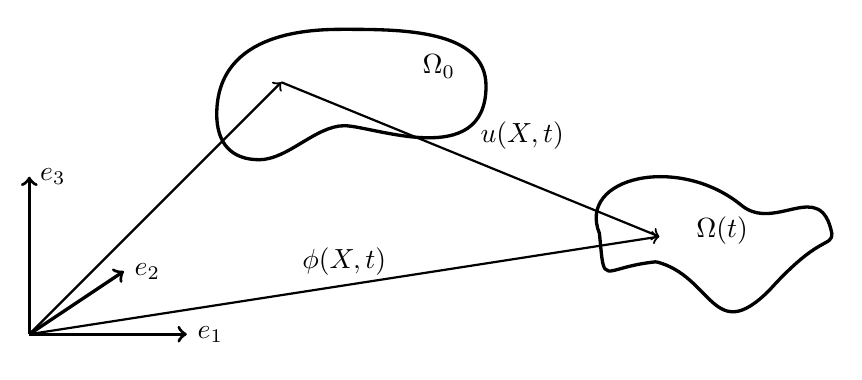
\begin{tikzpicture}[scale=0.8]
  %\draw[step=1.0,black,thin] (-3.,-1.) grid (3,4.);
  %\draw (-3,-1) -- (3,-1) -- (3,4) -- (-3,4) -- (-3,-1);
  \draw[very thick,->] (-5,-2.5) -- (-2.5,-2.5) node [right] {$\vect{e}_1$};
  \draw[very thick,->] (-5,-2.5) -- (-5,0.) node [right] {$\vect{e}_3$};
  \draw[very thick,->] (-5,-2.5) -- (-3.5,-1.5) node [right] {$\vect{e}_2$};
  \begin{scope}[scale=0.45]
    \draw[very thick] (-3,0.6) .. controls +(1,0) and +(-1,0) .. (0,1.8)  
    .. controls +(1,0) and +(0,-3) .. (5,3.2) 
    .. controls +(0,2) and +(2,0)  .. (0,5.2) 
    .. controls +(-1,0) and +(0,3) .. (-4.5,2.2) 
    .. controls +(0,-1) and +(-1,0).. (-3,0.6) ;
  \end{scope}
  \node at (1.5,1.75) {$\Omega_0$};
  %% Deformed body +2.
  \begin{scope}[scale=0.9]
    \draw[very thick] (0.+0.5+5.,0-1.5) ..controls (1.+0.5+5.,-0.25-1.5) and (1.+0.5+5.,-1.5-1.5) .. (2.+0.5+5.,-0.5-1.5) ..controls (2.9+0.5+5.,0.5-1.5) and (3.1+0.5+5.,0.25-1.5) .. (3.1+0.5+5.,0.5-1.5) ..controls (2.9+0.5+5.,1.5-1.5) and (2.1+0.5+5.,.5-1.5) .. (1.5+0.5+5.,1.-1.5) ..controls (0.4+0.5+5.,1.9-1.5) and (-1.4+0.5+5.,1.5-1.5) .. (-1.+0.5+5.,0.5-1.5)..controls (-0.4+0.+5.,-0.-2.) and (-1+0.5+5.,0.4-2.) .. (0+0.5+5.,0-1.5);
  \end{scope}
  \node at (6.,-0.85) {$\Omega(t)$};
  \draw[->,thick] (-5,-2.5) -- (-1.,1.5) node [midway,left] {$\X$};
  \draw[->,thick] (-5,-2.5) -- (5.,-0.95) node [midway,above] {$\vect{\phi}(\vect{X},t)$};
  \draw[->,thick] (-1.,1.5) -- (5.,-0.95) node [midway,above right] {$\vect{u}(\vect{X},t)$};
\end{tikzpicture}

%%% Local Variables:
%%% mode: latex
%%% TeX-master: "../../mainManuscript"
%%% End:
  \caption{Deformation of a solid body between a reference state $\Omega_0$ to a subsequent state $\Omega_t$.}
  \label{fig:deformationFunction}
\end{figure}

In the reference configuration, every material particle is located by their position vectors: $\vect{X}=X_\alpha \vect{e}_\alpha$, where $X_\alpha$ denotes the \textit{Lagrangian coordinates} and $\vect{e}_\alpha$ the basis vectors. At a subsequent time $t$, the particle initially located at $\vect{X}$ may have moved and its current location is given by the smooth mapping $\vect{\phi}(\vect{X},t)=\phi_i(\vect{X},t)\vect{e}_i$. Thus, the mapping $\vect{\phi}$ provides the paths of every particle of the solid during the deformation. In the lagrangian coordinates system, every particles are tracked during the deformation while the \textit{Eulerian coordinates}, denoted by $\vect{x}=x_i\vect{e}_i$, correspond to a \textit{spatial description}.
Note that in the above definitions Greek indices are used for quantities evaluated in the reference configuration whereas Latin ones refer to quantities defined in the current configuration. 

The \textit{displacement} and \textit{velocity} vectors of a particle between the reference and the current configuration are respectively:
\begin{align}
    &\vect{u}(\vect{X},t)=\vect{\phi}(\vect{X},t) - \vect{X} \qquad \forall\:\: \vect{X},t \in \Omega_0\times \tau  \label{eq:displacement}\\
    &\vect{v}(\vect{X},t)=\drond{\vect{\phi}}{t}(\vect{X},t) = \vect{\dot{\phi}}(\vect{X},t) \qquad  \forall\: \: \vect{X},t \in \Omega_0\times \tau  \label{eq:velocity}
\end{align}
where the superposed dot denotes the material time derivative. Then, the second-order two-point \textit{deformation gradient} tensor is defined as:
\begin{equation}
  \label{eq:F_phi}
    \tens{F}=\nablat_0 \vect{\phi} (\vect{X},t)
\end{equation}
where $\nablat_0 (\bullet)$ refers to the gradient operator on the reference configuration. This tensor can also be written by using equation \eqref{eq:displacement}:
\begin{equation}
  \tens{F}= \nablat_0 \vect{u}(\vect{X},t) + \tens{I} \label{eq:F_displacement}
\end{equation}
with $\tens{I}$, the second-order identity tensor. The deformation gradient tensor characterizes the variations of lengths, areas and volumes. Indeed, the infinitesimal vector, oriented surface and volume elements respectively denoted by $\vect{dX},\vect{dS}$ and $dV$ and defined in the reference configuration transorm respectively to:
\begin{equation}
  \label{eq:transport_equations}
  \begin{aligned}
    & dx_i=F_{i\alpha}dX_\alpha \\
    & ds_i=J F_{\alpha i}^{-1}dS_{\alpha} \\
    & dv=JdV 
  \end{aligned}
\end{equation}
in the current configuration. The transport equations \eqref{eq:transport_equations} involve the determinant of the deformation gradient $J=\det(\tens{F})>0$, also called the \textit{Jacobian of the deformation}. The deformation gradient is a strain measure since it accounts for changes in lengths and angles (\textit{i.e. the change of shape of a body}). Other strain measures can be used such as the \textit{right Cauchy-Green} or the \textit{Green-Lagrange} tensors, respectively defined as:
\begin{equation*}
   \tens{C}=\tens{F}^T\tens{F} \quad ; \quad \tens{E}=\frac{1}{2}(\tens{C}-\tens{I})
\end{equation*}
where $\tens{I}$ is the second-order identity tensor. The Green-Lagrange tensor can also be written by means of equation \eqref{eq:F_displacement}:
\begin{equation*}
  \tens{E}=\frac{1}{2}(\nablat_0 \vect{u} + \nablat_0 \vect{u}^T + \nablat_0 \vect{u}\nablat_0 \vect{u}^T)
\end{equation*}
In particular, when the deformation involves displacement vectors such that $\norm{\nablat_0 \vect{u}} \ll 1$, the last (second-order) term of the previous definition can be neglected leading to:
\begin{equation}
  \label{eq:epsilon}
  \tens{E} \approx \frac{1}{2}(\nablat_0 \vect{u} + \nablat_0 \vect{u}^T) = \tens{\eps}
\end{equation}
with $\tens{\eps}$ the \textit{linearized strain tensor}, the symmetric part of the displacement gradient. Such deformations fall in the \textit{linearized geometrical framework} or \textit{infinitesimal theory} and are characterized by small strain but possibly large displacements. Furthermore, when the deformation leads to a displacement vector $\norm{\vect{u}} \ll 1$ reference and current configurations are considered as indentical. These situations correspond to the \textit{small strain} framework for which the reference and current configurations are considered as identical.

\subsection{Balance equations}
In this section a solid domain $\Omega(t)$ undergoing a deformation is still considered within the time interval $\tau = \[0,T\]$. According to the formulation adopted in \cite{Plohr}, time derivatives of geometrical relations \eqref{eq:F_phi} and \eqref{eq:epsilon} combined to the definition of the velocity field \eqref{eq:velocity} yields kinematic conservations laws. Those conservation laws reads respectively:
\begin{align}
  & \tens{\dot{F}} - \nablat_0\vect{v} = \tens{0} \label{eq:HE_kinematic}\\
  & \tens{\dot{\eps}} - \nablat^s\vect{v} = \tens{0} \label{eq:HPP_kinematic}
\end{align}
where $\nablat^s$ denotes the symmetric gradient operator.

Then, we consider the conservation of mass in the continuum during the deformation in integral form:
\begin{equation*}
  \int_\Omega \rho d\Omega = \int_{\Omega_0} \rho_0 d\Omega \qquad \forall \: t \in  \tau
\end{equation*}
which, with the third transport formula reads:
\begin{equation}
  \label{eq:mass_conservation_law}
  \int_{\Omega_0} \(J\rho - \rho_0\) d\Omega = 0
\end{equation}
Leading to the first balance equation, namely the local conservation of mass:
\begin{equation}
  \label{eq:mass_balance}
  \rho = \frac{\rho_0}{J} \qquad \forall \: \vect{X},t \: \in \Omega_0\times \tau
\end{equation}
In particular, the linearised geometrical framework automatically satisfies this relation since current and reference configurations are the same (\textit{i.e.} $\rho=\rho_0 \: \forall t\in\tau$).

We now move on to the equilibrium between acceleration effects, namely \textit{intertia}, and external forces undergone by a solid $\Omega$. This conservation law corresponds to \textit{Newton's second law}:
\begin{equation*}
  \int_\Omega \rho \vect{\dot{v}} d\Omega = \int_{\partial \Omega} \vect{t} dS + \int_{\Omega} \rho\vect{b}d\Omega \qquad \forall \: t \in  \tau
\end{equation*}
where $\vect{t}$ denotes surface forces and $vect{b}$ volume forces in the current configuration. We then introduce the symmetric second-order \textit{Cauchy stress tensor} $\tens{\sigma}$ by using Cauchy's theorem $\vect{t}=\tens{\sigma}\cdot \vect{n}$ where $\vect{n}$ is the outwerd normal vector to the surface element $dS$. 

For further developments, the divergence theorem is required:
\begin{equation}
  \label{eq:Ostrogradski_th}
  \int_{\partial \Omega} (\bullet)\cdot \vect{dS}=\int_\Omega \nablav \cdot (\bullet) \: d\Omega
\end{equation}
where $\nablav \cdot (\bullet)$ denotes the divergence operator on the current configuration. Introduction of the previous formula in the second law of Newton leads to:
\begin{equation}
  \label{eq:Linear_momentum_conservation_eulerian}
  \int_{\Omega} \( \rho \vect{\dot{v}} - \nablav \cdot \tens{\sigma} -  \rho\vect{b} \) d\Omega = \vect{0} \qquad \forall \:t \in  \tau
\end{equation}
Conservation law \eqref{eq:Linear_momentum_conservation_eulerian} can be mapped to the reference configuration by using the transport formula of volume elements and the mass balance equation \eqref{eq:mass_balance}, thus yielding:
\begin{equation}
  \label{eq:Linear_momentum_conservation}
  \int_{\Omega_0} \( \rho_0 \vect{\dot{v}} - J \nablav \cdot \tens{\sigma} -  \rho_0\vect{b} \) d\Omega = \vect{0} \qquad \forall \: t \in\tau
\end{equation}
In equation \eqref{eq:Linear_momentum_conservation}, the divergence operator on the current configuration can be transported to the reference one by means of the \textit{Piola transform}:
\begin{definition}
  The Piola-Kirchhoff tranform $\tens{T}^P$ of a second-order tensor $\tens{T}$ is defined as:
  \begin{equation*}
    \tens{T}^P=J\tens{T}\cdot\tens{F}^{-1}
  \end{equation*}
  and satisfies:
  \begin{equation*}
    \nablav_0\cdot \tens{T}^P = J \nablav \cdot \tens{T}
  \end{equation*}
  where $\nablav_0\cdot (\bullet)$ is the divergence operator on the reference configuration.
\end{definition}
Another stress measure that corresponds to the Piola transform of Cauchy stress tensor is thus introduced, the \textit{first Piola-Kirchhoff stress tensor (PK1)} $\tens{\Pi}=J\tens{\sigma}\cdot\tens{F}^{-1}$. Hence, the vanishing of the integrand in equation \eqref{eq:Linear_momentum_conservation} yields the balance equation of the \textit{lagrangian linear momentum}:
\begin{equation}
  \label{eq:Lagrangian_linear_momentum}
  \rho_0 \vect{\dot{v}} - \nablav_0 \cdot \tens{\Pi} = \rho_0 \vect{b} \qquad \forall \: \: \vect{X},t \in \Omega_0 \times \tau 
\end{equation}
When considering deformations within the small strain framework the balance equation of linear momentum can be deduced from equation \eqref{eq:Linear_momentum_conservation_eulerian}, leading to:
\begin{equation}
  \label{eq:HPP_linear_momentum}
  \rho_0 \vect{\dot{v}} - \nablav \cdot \tens{\sigma} = \rho_0 \vect{b}  \qquad \forall \: \: \vect{x},t \in \Omega \times \tau 
\end{equation}

We complete the set of balance laws by considering the conservation of the energy of a system, also known as the \textit{first law of thermodynamics}. This law relates a balance between the rates of change of \textit{kinetic} and \textit{internal} energies, the power of external forces and the amount of heat entering the system as \textit{volume} or \textit{surface heat sources}.
\begin{equation*}
  \ddroit{}{t}\int_{\Omega} \(\frac{1}{2}\rho \vect{v}\cdot\vect{v} + \rho e\) d\Omega = \int_{\partial \Omega} \(\tens{\sigma}\cdot\vect{n}\)\cdot\vect{v} \: dS + \int_{\Omega} \rho\vect{b}\cdot\vect{v} \: d\Omega + \int_{\Omega} \rho r \:d\Omega - \int_{\partial \Omega} \vect{q}\cdot\vect{n} \: dS \qquad \forall \: t \in  \tau 
\end{equation*}
where $\vect{q}$ is the outward heat flux vector and $r$ is a volume heat source. By using the divergence theorem \eqref{eq:Ostrogradski_th}, the previous equation reads:
\begin{equation*}
\ddroit{}{t}\int_{\Omega} \(\frac{1}{2}\rho \vect{v}\cdot\vect{v} + \rho e\) d\Omega = \int_{\Omega} \(\nablav\cdot(\tens{\sigma}\cdot\vect{v}) +  \rho\vect{b}\cdot\vect{v} \) d\Omega + \int_{\Omega} \rho r \: d\Omega  - \int_{\partial \Omega} \vect{q}\cdot\vect{n} \: dS \qquad \forall \: t \in  \tau 
\end{equation*}
The transport of this relation on the reference configuration based on \eqref{eq:transport_equations} allows to introduce the time derivative of the left-hand side in the integral
\begin{equation*}
\int_{\Omega_0} \(\rho_0 \vect{\dot{v}} + \rho_0 \dot{e}\) d\Omega = \int_{\Omega_0} \(J\nablav\cdot(\tens{\sigma}\cdot\vect{v}) +  \rho_0\vect{b}\cdot\vect{v} \) d\Omega + \int_{\Omega_0} \rho_0 r \:d\Omega- \int_{\partial \Omega_0} J\vect{q}\cdot \tens{F}^{-1}\cdot\vect{n} \: dS \qquad \forall \: t \in  \tau 
\end{equation*}
Then, substitution of the linear momentum according to equation \eqref{eq:Lagrangian_linear_momentum} yields, after some algebra, the conservation law of internal energy:
\begin{equation}
  \label{eq:conservation_law_energy}
  \int_{\Omega_0} \rho_0 \dot{e} d\Omega = \int_{\Omega_0} \tens{\Pi}:\nablat_0\vect{v}\: d\Omega + \int_{\Omega_0} \(\rho_0r  - \nablav_0 \cdot \vect{Q}\) d\Omega \qquad \forall \: t \in  \tau 
\end{equation}
where $\vect{Q}=J\vect{q}\cdot \tens{F}^{-1}$ is the lagrangian heat flux vector. We thus deduce the balance equation of internal energy on the reference configuration:
\begin{equation}
  \label{eq:energy_balance}
  \rho_0 \dot{e} -  \tens{\Pi}:\nablat_0\vect{v}  + \nablav_0 \cdot \vect{Q}  = \rho_0 r \qquad \forall \: \: \vect{X},t \in \Omega_0 \times \tau 
\end{equation}
where $\nablat_0\vect{v} = \tens{\dot{F}}$. Finally, the small strain version of equation \eqref{eq:energy_balance} is: 
\begin{equation}
  \label{eq:energy_balance_euler}
  \rho_0 \dot{e} -  \tens{\sigma}:\nablat^{s} \vect{v}  + \nablav \cdot \vect{q}  = \rho_0 r \qquad \forall \: \: \vect{x},t \in \Omega \times \tau 
\end{equation}
in which $\nablat^{s} (\bullet)$ denotes the symmetric part of the gradient, in particular: $\nablat^s \vect{v} = \tens{\dot{\eps}}$. Stress measures are conjugate to strain measures through the power. In what follows, stress and strain may respectively be refered to as \textit{thermodynamic forces} and \textit{internal variables} according to the thermodynamics framework. The former obey a \textit{state equation} while the latter describe the evolution of the thermodynamic system. 
\subsection{Constitutive equations -- Thermodynamics}
The closure of a problem is given by the constitutive equations (\textit{i.e state laws}) for the stress. Once and for all, we consider here constitutive models within the \textit{Generalized Standard Materials} (GSM) framework \cite{GSM}.

\subsubsection*{The general (hyper)elasticity formulation}
First, the \textit{Clausius-Duhem} inequality resulting from combination of first and second laws of thermodynamics, reads: 
\begin{equation}
  \label{eq:Clausius-Duhem}
  \underbrace{\phantom{\frac{1}{\theta}} \tens{\Pi}:\tens{\dot{F}} + \rho_0 \(\theta \dot{\eta} -\dot{e}\)}_{\Dscr^{int}} \:-\:  \underbrace{\frac{1}{\theta} \vect{q} \cdot \nablav_0 \theta}_{-\Dscr^{th}} \geq 0  \qquad \forall \: \: \vect{X},t \in \Omega_0 \times \tau 
\end{equation}
where $\Dscr^{int}$ and $\Dscr^{th}$ are respectively the specific mechanical and thermal dissipations. Equation \eqref{eq:Clausius-Duhem} results in vanishing dissipations for \textit{reversible} processes and in a strict inequality for \textit{irreversible} ones. Furthermore, a widely used assumption consists in considering that the mechanical and thermal dissipations simultaneously satisfy non-negativeness. Note that the \textit{Fourier's law} of conduction is based on the non-negativeness of the thermal dissipation and leads to the following definition of the heat flux vector in order to ensure the positivity of the thermal dissipation:
\begin{equation*}
  \label{eq:Fourier_law}
  \vect{q}=-\tens{k}\cdot\nablav_0 \theta
\end{equation*}


The internal energy density is a function of strain, \textit{entropy} $\eta$ and additional state variables $\Vc_p, \: (1\leq p \leq N)$ describing irreversible processes. Recall that calligraphic symbols denote column array. It is more convenient to use its \textit{Legendre transform}, the \textit{Helmholtz free energy density potential} $\psi\(\tens{F},\theta,\Vcb\)=e\(\tens{F},\eta,\Vcb\)-\theta \eta$ where $\theta$ is the temperature. The free energy density is supposed \textit{objective} or \textit{frame indifferent} \cite[p.255]{Simo}, concave with respect to temperature and convex with respect to other variables. The mechanical dissipation can then be rewritten as:
\begin{equation*}
  \Dscr^{int} = \tens{\Pi}:\tens{\dot{F}} - \rho_0 \(\dot{\psi} +\eta \dot{\theta}\) 
\end{equation*}
The time derivative of Helmholtz free energy density:
\begin{equation}
  \label{eq:derivative_psi}
  \dot{\psi} = \drond{\psi}{\tens{F}}:\tens{\dot{F}} + \drond{\psi}{\theta}\dot{\theta} + \drond{\psi}{\Vcb}\dot{\Vcb}
\end{equation}
can be introduced within the mechanical dissipation so that one gets:
\begin{equation}
  \label{eq:Dint_psi_factor}
  \Dscr^{int} = \(\tens{\Pi}- \rho_0 \drond{\psi}{\tens{F}} \):\tens{\dot{F}} - \rho_0 \(\drond{\psi}{\theta} +\eta\) \dot{\theta}  - \rho_0\drond{\psi}{\Vcb}\dot{\Vcb} 
\end{equation}


Since the mechanical dissipation must be non-negative regardless of the nature of the deformation, it must in particular vanish for a reversible isothermal process (\textit{i.e. $\theta=const$}) for which every additional internal variables are constant. With these considerations, we are left with the relation:
\begin{equation*}
  \( \tens{\Pi} - \rho_0\drond{\psi}{\tens{F}} \): \tens{\dot{F}} = 0
\end{equation*}
holding regardless of the deformation, and hence:
\begin{equation}
  \label{eq:PK1_definition}
  \rho_0\drond{\psi}{\tens{F}} = \tens{\Pi}
\end{equation}
A material is said \textit{hyperelastic} if there exist a \textit{stored energy function} $\rho_0\psi$ from which can be derived the first Piola-Kirchhoff stress tensor \cite[p.8]{Foundation_of_elasticity}. The time derivative of this relation leads to:
\begin{equation}
  \label{eq:HE_tangent}
  \tens{\dot{\Pi}} = \rho_0\ddrond{\psi}{\tens{F}}{\tens{F}}:\tens{\dot{F}} = \Hbb:\tens{\dot{F}} 
\end{equation}
where $\Hbb$ is the $4$th order \textit{tangent modulus} tensor. Equivalently we have for linear elasticity:
\begin{equation}
  \label{eq:Cauchy_definition}
  \rho_0 \drond{\psi}{\tens{\eps}} = \tens{\sigma}
\end{equation}
and:
\begin{equation}
  \label{eq:HPP_tangent}
  \tens{\dot{\sigma}} = \rho_0\ddrond{\psi}{\tens{\eps}}{\tens{\eps}}:\tens{\dot{\eps}} = \Cbb:\tens{\dot{\eps}} 
\end{equation}
In equation \eqref{eq:HPP_tangent}, $\Cbb$ is the $4$th order \textit{elastic stiffness} tensor which has major and minor symmetries. For isotropic elasticity, $C_{ijkl}=\lambda \delta_{ij}\delta_{kl} + \mu \(\delta_{ik}\delta_{jl}+\delta_{il}\delta_{jk}\)$ yields \textit{Hook's law} with $(\lambda,\mu)$ are Lamé parameters.

Similar considerations lead to the state laws for entropy and for additional thermodynamic forces :
\begin{equation}
  \label{eq:thermodynamic_forces}
  \drond{\psi}{\theta} = - \eta \quad ; \quad \rho_0\drond{\psi}{\Vcb}=\Acb
\end{equation}
where $\Acb$ are thermodynamic forces associated to internal variables $\Vcb$.
In what follows, we shall consider hyperelastic or linear elastic deformations that do not involve irreversible processes (\textit{e.g. damage or thermal softening}). Hence, additional internal variables and associated thermodynamic forces are not activated in such situations. However, the cases of \textit{elastoplasticity} and \textit{elasto-viscoplasticity}, involving such variables and forces, will be considered in the linearized geometrical framework.

\begin{remark}
  \label{rq:isothermal_deformation}
  Temperature has been introduced as an internal variable and requires the introduction of the heat equation for the closure of the system:
  \begin{equation*}
    \rho_0 C \dot{\theta} = \rho_0 r - \nablav_0 \cdot \vect{Q} - \rho_0 \drond{\psi}{\Vcb}\dot{\Vcb} + \theta \(\drond{\tens{\Pi}}{\theta}:\tens{\dot{F}} - \drond{\Acb}{\theta}\dot{\Vcb} \)
  \end{equation*}
  Nevertheless, we will restrict our attention in the following to isothermal deformation so that temperature can be omitted and internal energy balance equation \eqref{eq:energy_balance} or \eqref{eq:energy_balance_euler} is automatically satisfied. Indeed, for isothermal processes the heat equation leads to:
  \begin{equation*}
    \rho_0 r - \nablav_0 \cdot \vect{Q} = \rho_0 \drond{\psi}{\Vcb}\dot{\Vcb}
  \end{equation*}
  which, once introduced in the energy balance \eqref{eq:energy_balance} yields:
  \begin{equation*}
    \rho_0 \dot{e} - \tens{\Pi}:\tens{\dot{F}} = \rho_0 \drond{\psi}{\Vcb}\dot{\Vcb}
  \end{equation*}
  By using the free energy density time derivative \eqref{eq:derivative_psi} and noting that $\eta=-\drond{\psi}{\theta} =0$, we get that each side of the previous equation vanishes.
\end{remark}


\subsubsection*{History-dependent models in small strain}
While elasticity does not involve dissipation, plasticity is characterized by irreversible strain and hardening variables $\Vcb$ that account for the loading history undergone by every material particles. Within the linearized geometrical framework, the infinitesimal strain tensor $\tens{\eps}$ is assume to be additively decomposed into an elastic and a plastic part:
\begin{equation}
  \label{eq:additive_plast}
  \tens{\eps} = \tens{\eps}^e + \tens{\eps}^p
\end{equation}
such that the mechanical dissipation only involve the plastic part:
\begin{equation}
  \label{eq:HPP_dissipation}
  \Dscr^{int}=\tens{\sigma}:\tens{\dot{\eps}}^p -\rho_0 \drond{\psi}{\Vcb}\dot{\Vcb} \geq 0
\end{equation}

A \textit{yield condition} is defined with the \textit{yield function} $f(\tens{\sigma},\Acb)$ so that that the elastic domain $\Ebb$ in stress space $(\tens{\sigma},\Acb)$ corresponds to:
\begin{equation}
  \label{eq:elastic_convex}
  \Ebb = \{ (\tens{\sigma},\Acb)\: | \: f(\tens{\sigma},\Acb) \leq 0\}
\end{equation}
According to the GSM framework \cite{GSM} we assume the existence of a dissipation pseudo-potential $\Phi(\tens{\sigma},\Vcb)$, convex with respect to thermodynamic forces and vanishing at the origin of the $(\tens{\sigma},\Vcb)$ space. This pseudo-potential enables the derivation of the plastic \textit{flow} and \textit{hardening} rules:
\begin{subequations}
  \begin{alignat}{2}
    \label{eq:flow_rule_plast}
     \tens{\dot{\eps}}^p&=&&\drond{\Phi}{f}\drond{f}{\tens{\sigma}}\\
    \label{eq:hardening_rule_plast}
     \dot{\Vcb}& = -&&\drond{\Phi}{f}\drond{f}{\Acb}
  \end{alignat}
\end{subequations}
where $\drond{\Phi}{f}=\dot{p}$ is the \textit{plastic multiplier}. We then distinguish two cases:
\begin{itemize}
\item \textbf{Rate-independent} plasticity is based on the assumption that admissible thermodynamic forces lie within the elastic domain \eqref{eq:elastic_convex}. The plastic multiplier is used as a Lagrange multiplier in order to ensure $f(\tens{\sigma},\Acb)\leq 0$ and must obey the \textit{K{\"u}hn-Tucker compatibility conditions}:
\begin{equation}
  \label{eq:Kuhn_Tucker}
  \dot{p} \geq 0 \quad ; \quad f \leq 0 \quad ; \quad \dot{p}f =0 
\end{equation}
The plastic multiplier, or the \textit{equivalent plastic strain rate} is determined by the \textit{consistency condition}:
\begin{equation}
  \label{eq:consistency_condition}
  \dot{f}=0
\end{equation}

% In analogy with the elastic law \eqref{eq:HPP_tangent}, rate-independent plastic evolutions are governed by the \textit{elastoplastic tangent modulus}:
% \begin{equation}
%   \label{eq:HPP_tangent_plasticity}
%   \tens{\dot{\sigma}}=\Cbb^{ep}:\tens{\dot{\eps}}
% \end{equation}

\item \textbf{Viscoplasticity} or \textbf{rate-dependent} plasticity can be seen as a regularization of rate-independent plasticity that relaxes the condition $f(\tens{\sigma},\Acb)\leq 0$ and thus leads to admissible thermodynamic forces outside the elastic domain \cite[p.58]{Simo}. Furthermore, the plastic fluxes $\tens{\dot{\eps}}^p, \dot{\Vcb}$ are completely determined by the knowlegde of the dissipation pseudo-potential. 
\end{itemize}
\subsubsection*{Examples of constitutive laws}
We now specify the above discussion to constitutive models that will be used in the following of the manuscript.

$\newline$
\textbf{The neo-Hookean hyperelastic model} is well-suited to describe rubber-like materials and is based on the polyconvex stored energy function:
\begin{equation}
  \label{eq:neo-hook_energy}
  \rho_0 \psi(J,\tens{F})= \frac{\kappa}{2}(J-1)^2 + \frac{\mu}{2}\[J^{-2/3} (\tens{F}:\tens{F})-3 \]
\end{equation}
where $\kappa$ is the bulk modulus and $\mu$ the Lam\'e shear modulus. We then introduce the \textit{tensor cross product} \cite{cross_tensor_product} of two second order two-point tensors $\tens{a}$ and $\tens{c}$, defined as:
\begin{equation}
  \label{eq:cross_tensor_product}
  \(\tens{a} \tens{\times} \tens{c}\)_{i\alpha}= \Ec_{ijk} \Ec_{\alpha \beta \gamma} a_{j\beta}b_{k\gamma}
\end{equation}
where $\Ec_{ijk}$ is the \textit{Levi-Civita} permutation symbol. By making use of this operator, the Jacobian $J$ can be written:
\begin{equation*}
  J=\frac{1}{6}\(\tens{F}\ttimes\tens{F}\):\tens{F}
\end{equation*}
or equivalently 
\begin{equation*}
  J=\frac{1}{3}\tens{H}:\tens{F}
\end{equation*}
in which $\tens{H}=\frac{1}{3}\tens{F}\ttimes\tens{F}=J\tens{F}^{-T}$ is the \textit{adjoint tensor} of the deformation gradient. Note that by using the tensor cross product operator, one can easily show that $\drond{J}{\tens{F}}=\tens{H}$. With these definitions, the derivative of the stored energy function \eqref{eq:neo-hook_energy} with respect to the deformation gradient can be computed so that the PK1 tensor can be derived:
\begin{equation}
  \label{eq:PK1_neo-hook}
  \tens{\Pi} = \mu J^{-2/3} \[\tens{F}- \frac{1}{3}\(\tens{F}:\tens{F}\) \tens{F}^{-T}\] + \kappa \(J-1\)\tens{H}
\end{equation}

The acoustic tensor $A_{ij}=N_\alpha H_{i\alpha j\beta} N_\beta$ for the neo-Hookean hyperelastic model is \cite{Haider_FVM}:
\begin{equation}
  \label{eq:neo-hook_acoustic}
  \begin{split}
      \tens{A}=\[\frac{5}{9}\mu J^{-8/3}\(\tens{F}:\tens{F}\)   + \kappa \]&(\tens{H}\cdot\vect{N})\otimes\(\tens{H}\cdot\vect{N} \)  + \mu J^{-2/3} \tens{I}  \\ &-\frac{2}{3}\mu J^{-5/3}\[(\tens{H}\cdot\vect{N})\otimes\(\tens{F}\cdot\vect{N} \)	+  (\tens{F}\cdot\vect{N})\otimes\(\tens{H}\cdot\vect{N} \)\]
  \end{split}
\end{equation}
The polyconvexity of this model ensures the positive definiteness of the acoustic tensor \eqref{eq:neo-hook_acoustic} \cite{Kluth}.

$\newline$
\textbf{The Saint-Venant-Kirchhoff hyperelastic model} is an extension of linear elastic Hook's law to hyperelasticity with a stored energy function that takes the form:
\begin{equation}
  \label{eq:SVK_energy}
  \rho_0\psi=\frac{1}{8}\(\tens{F}^T\tens{F}- \tens{I}\):\Cbb:\(\tens{F}^T\tens{F}- \tens{I}\)
\end{equation}
where $\Cbb$ is the elasticity tensor. In a similar manner as for the neo-Hookean model, the expression of the PK1 tensor is:
\begin{equation}
  \label{eq:SVK_PK1}
  \tens{\Pi} = \frac{1}{2}\lambda \(\tens{F}:\tens{F}- 3\) \tens{F} + \mu\tens{F}\(\tens{F}^T\tens{F}- \tens{I}\)
\end{equation}
The tangent modulus is then obtained by deriving this stress tensor:
\begin{equation}
  \label{eq:SVK_tangent}
  \Hbb = \lambda \[\tens{F}\otimes\tens{F} + \frac{1}{2} (\tens{F}:\tens{F}- 3)\Ibb\]+ \mu\(\Abb- \Ibb \)
\end{equation}
with $A_{i\alpha j \beta}=F_{k\alpha}F_{k\beta}\delta_{ij} + F_{j\alpha}F_{i\beta} +F_{i\mu} F_{j\mu}\delta_{\alpha\beta}$ and the fourth order identity tensor $I_{i\alpha j \beta}=\delta_{ij}\delta_{\alpha \beta}$. The previous tangent modulus finally leads to the acoustic tensor:
\begin{equation}
  \label{eq:SVK_acoustic}
  \begin{split}
    \tens{A} = \lambda \[\vphantom{\frac{1}{2}} (\tens{F}\cdot\vect{N})\otimes(\tens{F}\cdot\vect{N}) \right.+ &\left.\frac{1}{2} (\tens{F}:\tens{F}- 3)\tens{I}\] \\
    + & \mu\[(\tens{F}\cdot\vect{N})\cdot(\tens{F}\cdot\vect{N})\tens{I} + (\tens{F}\cdot\vect{N})\otimes(\tens{F}\cdot\vect{N}) + \tens{F}\cdot\tens{F}^T- \tens{I} \]
  \end{split}
\end{equation}
Even though it is known that this model can lead to non-physical solutions for very large deformation, it will be used for a one-dimensional strain problem for it enables to easily develop an analytical solution.  


$\newline$
\textbf{The plastic $J_2$ flow theory}, generally used to model metals, involves a yield function $f$ based on the second invariant of Cauchy stress deviatoric part $J_2=\tens{s}:\tens{s}$, where $\tens{s}=\tens{\sigma}-\frac{1}{3}\tr \tens{\sigma}$.
By considering internal variables and associated forces as: $\{\Vcb,\Acb\}=\{\[\tens{\eps}^p,p\],\[\tens{s}-\tens{Y},-R(p)\]\}$, one defines the following Helmoltz free energy density:
%can describe \textit{isotropic} linear hardening by setting $\tens{Y}=\tens{0}$, and \textit{kinematic} linear hardening with $R(p)=0$.The Helmoltz free energy density here reads:
\begin{equation}
  \label{eq:EP_helmoltz}
  \rho \psi = \frac{1}{2}\tens{\eps}^e:\Cbb:\tens{\eps}^e + \frac{2}{3}C\tens{\eps}^p:\tens{\eps}^p + H(r)
\end{equation}
In this expression, $r$ is to be defined, $H''(r)$ is the \textit{isotropic hardening} modulus and $\tens{Y}$ describes the evolution of the elastic domain center in stress deviator space and is related to \textit{kinematic hardening}. Linear hardenings will be considered here by setting either $\tens{Y}=\tens{0}$ for isotropic or $R(r)=0$ for kinematic hardening. The definition of thermodynamic forces \eqref{eq:thermodynamic_forces} leads to:
\begin{subequations}
  \begin{alignat}{1}
    \label{eq:eta}
    \tens{Y}&=\frac{2}{3}C\tens{\eps}^p \\
    \label{eq:isotropic_hardening}
    R &=H'(r)
  \end{alignat}
\end{subequations}
Furthermore, the \textit{von-Mises yield surface} is defined as:
\begin{equation}
  \label{eq:von-Mises_yield}
  f\(\tens{\sigma},\Acb \)= \sqrt{\frac{3}{2}}\norm{\tens{s}-\tens{Y}} - \(R(r)+\sigma^y\) \equiv 0
\end{equation}
$\sigma^y$ being the traction yield stress. The specialization of flow rules \eqref{eq:flow_rule_plast},\eqref{eq:hardening_rule_plast} leads to:
\begin{subequations}
  \begin{alignat}{1}
    \label{eq:plastic_strain_rate}
    &\tens{\dot{\eps}}^p=\dot{p}\sqrt{\frac{3}{2}}\frac{\tens{s}-\tens{Y}}{\norm{\tens{s}-\tens{Y}}}=\dot{p}\:\sqrt{\frac{3}{2}}\tens{m} \\
    \label{eq:equiv_plastic_strain_rate}
    &\dot{r}=\dot{p}
  \end{alignat}
\end{subequations}
where $r$ is identified from \eqref{eq:equiv_plastic_strain_rate} as the equivalent plastic strain. Considering rate-independent plasticity and combining the elastic law $\tens{\dot{\sigma}}=\Cbb:\(\tens{\dot{\eps}}-\tens{\dot{\eps}}^p\)$ yields the following evolution law:
\begin{equation}
  \label{eq:p_evolution}
  \dot{p}=\sqrt{\frac{3}{2}}\frac{2\mu}{3\mu+\beta}\tens{m}:\tens{\dot{\eps}}
\end{equation}
where $\beta=C$ for kinematic hardening and $\beta=R'(p)$ for isotropic hardening. Finally, equations \eqref{eq:plastic_strain_rate} and \eqref{eq:p_evolution}can be sequencially introduced in the elastic law so that one gets \cite[eq (2.2.22)]{Simo}:
\begin{equation}
  \label{eq:elastoplastic_tangent}
  \tens{\dot{\sigma}}=\(\Cbb - \frac{6\mu^2}{3\mu +\beta}\tens{m}\otimes\tens{m} \):\tens{\dot{\eps}} = \Cbb^{ep}:\tens{\dot{\eps}}
\end{equation}
with $\Cbb^{ep}$ the \textit{elastoplastic tangent modulus}. Note that (positive) linear hardenings ensure the positive definiteness of the elastoplastic acoustic tensor $\tens{A}^{ep}=\tens{A}^{elast} -  \frac{6\mu^2}{3\mu +\beta} (\tens{m}\cdot{n})\otimes(\tens{m}\cdot{n})$.  

Viscoplasticity on the other hand, leads to an explicit definition of the equivalent plastic strain:
\begin{equation}
  \label{eq:EVP_creep_law}
  \dot{p}=\left\langle \frac{f}{\eta}\right\rangle^n
\end{equation}
where $\left\langle\bullet\right\rangle=\frac{\bullet + \abs{\bullet}}{2}$ is the positive part function, and $n$ and $\eta$ are parameters arrising from the relaxation of the condition $f\leq 0$. Hence, rate-dependent plasticity is driven by the elastic law in which $\tens{\dot{\eps}^p}$ is given by \eqref{eq:flow_rule_plast} and \eqref{eq:EVP_creep_law}. 

\subsection{The general formulation}
We now summarize the conservation and constitutive laws obtained previously. Recall that the deformations considered here are isothermal and that history-dependent materials will be taken into account within linearized geometrical framework only. 
\subsubsection*{Linear elasticity and elasto-viscoplasticity}
We first gather the governing equations of elasticity and elasto-viscoplasticity within the linearized geometrical framework namely, the elastic law \eqref{eq:HPP_tangent}, the balance equation of linear momentum \eqref{eq:HPP_linear_momentum} and the kinematic law \eqref{eq:HPP_kinematic} which are repeated here for convenience:
\begin{align*}
  & \rho_0 \vect{\dot{v}} - \nablav \cdot \tens{\sigma} = \rho_0 \vect{b} \\
  & \tens{\dot{\sigma}} - \Cbb :\(\tens{\dot{\eps}}-\tens{\dot{\eps}}^p\) =\tens{0}\\
  & \tens{\dot{\eps}}-\nablat^s \vect{v} =\tens{0} \quad \qquad \forall \: \: \vect{x},t \in \Omega \times \tau 
\end{align*}
Note that the gradient operator of a vector $\vect{a}$ can be rewritten as a divergence operator:
\begin{equation}
  \label{eq:grad_div}
  \nablat \vect{a} = \nablav \cdot \(\vect{a}\otimes\tens{I} \)
\end{equation}
Hence, introduction of kinematic laws in the linear momentum balance yields, by assuming a cartesian coordinates system, the following \textit{conservative form}:
\begin{equation}
  \label{eq:general_conservative}
  \Qcb_t + \sum_{i=1}^D \drond{\Fcb\cdot \vect{e}_i}{x_i} = \Scb
\end{equation}
where the vector of conserved quantities $\Qcb$, fluxes vectors $\Fcb\cdot \vect{e}_i$ and the source term $\Scb$ are:
\begin{equation}
  \label{eq:vectors_elasticity}
  \Qcb =\matrice{\vect{v} \\ \tens{\sigma}} \quad ; \quad \Fcb\cdot\vect{e}_i = \matrice{-\frac{1}{\rho_0}\tens{\sigma}\cdot\vect{e}_i\\-\Cbb:\frac{\vect{v}\otimes\vect{e}_i +\vect{e}_i \otimes\vect{v} }{2} } \quad ; \quad \Scb = \matrice{ \vect{b} \\ -\Cbb:\tens{\dot{\eps}}^p}
\end{equation}
The quasi-linear form of equation \eqref{eq:general_conservative} is written by using the chain rule:
\begin{equation}
  \label{eq:HPP_quasi-linear}
  \Qcb_t + \Absf^i \drond{\Qcb}{x_i} = \Scb
\end{equation}
where:
\begin{equation*}
  \Absf^i=\drond{\Fcb\cdot \vect{e}_i}{\Qcb}=-\matrice{\tens{0}^3 & \frac{1}{\rho_0}\tens{I}\otimes\vect{e}_i\\\Cbb\cdot\vect{e}_i & \tens{0}^4}
\end{equation*}
in which symmetries of the elastic stiffness tensor have been used and $\tens{0}^p$ is a $p$th order null tensor. Since the elastic stiffness tensor is constant, system \eqref{eq:HPP_quasi-linear} is linear for elasticity and semi or non-linear for elasto-viscoplasticity depending on the flow rule
\eqref{eq:flow_rule_plast}.
\subsubsection*{Elasto-plasticity and hyperelasticity}
The non-linear constitutive equations of elastoplasticity and hyperelasticity prevent the straightforward writing of a conservative form. Indeed, such a conservation laws system is instead based on kinematic laws \eqref{eq:HE_kinematic} or \eqref{eq:HPP_kinematic}.
% \begin{align}
%   & \tens{\dot{F}} - \nablat_0 \vect{v} = \tens{0} \\
%   & \tens{\dot{\eps}} - \nablat^s\vect{v}=\tens{0} 
% \end{align}
Then, a conservative form \eqref{eq:general_conservative} is also written:
\begin{equation}
  \label{eq:general_conservative2}
  \Wcb_t + \sum_{i=1}^D \drond{\Fcb\cdot \vect{e}_\alpha}{X_\alpha} = \Scb
\end{equation}
 with:
\begin{alignat}{4}
  \label{eq:vectors_hyperelasticity}
  &\Wcb =\matrice{\vect{v} \\ \tens{F}} \quad &&; \quad \Fcb\cdot\vect{e}_\alpha = \matrice{-\frac{1}{\rho_0}\tens{\Pi}\cdot\vect{e}_\alpha\\-\vect{v}\otimes\vect{e}_\alpha } \quad &&; \quad \Scb = \matrice{ \vect{b} \\ \tens{0}} \quad &&\text{ for hyperelasticity}\\
  &\label{eq:vectors_plasticity}
  \Wcb =\matrice{\vect{v} \\ \tens{\eps}} \quad &&; \quad \Fcb\cdot\vect{e}_i = \matrice{-\frac{1}{\rho_0}\tens{\sigma}\cdot\vect{e}_i\\-\frac{\vect{v}\otimes\vect{e}_i +\vect{e}_i \otimes\vect{v} }{2} } \quad &&; \quad \Scb = \matrice{ \vect{b} \\\tens{0}} \quad &&\text{ for elastoplasticity}
\end{alignat}

Quasi-linear form are then built by introducing an auxiliary vector $\Qcb$ and using the chain rule according to \cite{Trangenstein91}:
\begin{equation}
  \label{eq:quasi-linear_Trangenstein}
  \drond{\Qcb}{t} + \(\drond{\Wcb}{\Qcb}\)^{-1}\drond{\Fcb\cdot\vect{e}_\alpha}{\Qcb} \drond{\Qcb}{X_\alpha} = \(\drond{\Wcb}{\Qcb}\)^{-1}\Scb = \tilde{\Scb}
\end{equation}
with the auxiliary vectors for elastoplasticity and hyperelasticity respectively defined as:
\begin{equation}
  \label{eq:auxiliary_vectors}
  \Qcb=\matrice{\vect{v}\\\tens{\sigma}} \quad ; \quad \Qcb=\matrice{\vect{v}\\\tens{\Pi}}
\end{equation}

Denoting momentarily and generically the stress measures by $\tens{S}$ and the strain measures by $\tens{P}$ so that $\Wcb^T=\[\vect{v},\tens{P}\]$ and $\Qcb^T=\[\vect{v},\tens{S}\]$, the matrix $\drond{\Wcb}{\Qcb}$ and its inverse are:
\begin{equation*}
  \drond{\Wcb}{\Qcb}=\matrice{\tens{I} & \tens{0}^3 \\ \tens{0}^3  & \drond{\tens{P}}{\tens{S}}} \Rightarrow \(\drond{\Wcb}{\Qcb}\)^{-1}=\matrice{\tens{I} & \tens{0}^3 \\ \tens{0}^3  & \drond{\tens{S}}{\tens{P}}}
\end{equation*}
in which $\drond{\tens{S}}{\tens{P}}$ is the tangent modulus of the considered constitutive model. Moreover, the derivative of the flux vectors with respect to the auxiliary vector has two different expressions depending on the constitutive model due to the symmetric gradient used for the linearized geometrical framework. On gets for hyperelastic materials:
\begin{equation}
  \drond{\Fcb\cdot\vect{e}_\alpha}{\Qcb}=-\matrice{\tens{0}^2 & \frac{1}{\rho_0}\tens{I}\otimes\vect{e}_\alpha \\    \tens{I}\boxtimes \vect{e}_\alpha & \tens{0}^4}
\end{equation}
while elastoplasticity leads to:
\begin{equation}
  \drond{\Fcb\cdot\vect{e}_i}{\Qcb}=-\matrice{\tens{0}^2 & \frac{1}{\rho_0}\tens{I}\otimes\vect{e}_i \\  \frac{\tens{I}\boxtimes \vect{e}_i+\vect{e}_i\otimes\tens{I}}{2} & \tens{0}^4   }
\end{equation}
in which the operator $\tens{I}\boxtimes\vect{e}_i$ is the transpose on second and third indices of the classical tensor product: $\tens{I}\boxtimes\vect{e}_i=\delta_{jk} \vect{e}_j\otimes \vect{e}_i\otimes\vect{e}_k$.

Finally, the quasi-linear forms associated to hyperelastic problems and elastoplastic ones are respectively:
\begin{alignat}{2}
  & \Qcb_t + \Absf^\alpha \drond{\Qcb}{X_\alpha} = \tilde{\Scb} \qquad &&\text{with: }\Absf^\alpha = -\matrice{ \tens{0}^2 & \frac{1}{\rho_0}\tens{I}\otimes\vect{e}_\alpha \\ \Hbb\cdot\vect{e}_\alpha & \tens{0}^4} \label{eq:HE_quasilinear}\\
  & \Qcb_t + \Absf^i \drond{\Qcb}{x_i} = \tilde{\Scb} \qquad &&\text{with: }\Absf^i = -\matrice{\tens{0}^2 & \frac{1}{\rho_0}\tens{I}\otimes\vect{e}_i\\ \Cbb^{ep}\cdot \vect{e}_i & \tens{0}^4} \label{eq:EP_quasilinear}
\end{alignat}
where the symmetries of the elastic stiffness tensor have been used. Note that the dependence on $\Qcb$ of matrices $\Absf(\Qcb)$ has been omitted for simplicity

%%% Local Variables:
%%% mode: latex
%%% TeX-master: "../mainManuscript"
%%% End:



\section{Characteristic analysis}
\label{sec:characteristic_analysis}
The eigenspaces of conservation laws systems defined above will be now investigated. As we shall see, the characteristic structure of those problems may lead to different type of waves propagating within a medium. Finally, existing analytical solutions of one-dimensional problems \cite{Wang} will be reviewed and that of a one-dimensional problem involving a hyperelastic \textit{Saint-Venant-Kirchhoff} material will be developed in order to illustrate the identified wave structures.
\subsection{Characteristic structure of solutions}
For the sake of simplicity studies of finite deformation and linearized geometrical frameworks will be condensed in this part by using a generic stress measure $\tens{S}$ and vectors written in the reference configuration. Furthermore, instead of studying multi-dimensional conservation laws systems, we will focus without loss of generality on conservative forms \eqref{eq:general_conservative} projected on an arbitrary direction $\vect{N}=\[\vect{e}_1,\vect{e}_2,\vect{e}_3\]$ \cite[p.425-426]{Leveque}. In this direction, the quasi-linear forms determined above are rewritten as:
\begin{equation}
  \label{eq:normal_quasi}
  \Qcb_t + \Jbsf \drond{\Qcb}{X_N} = \Scb
\end{equation}
where $X_N=\vect{X}\cdot\vect{N}$ and the \textit{Jacobian matrix} $\Jbsf = \Absf^\alpha N_\alpha$ arise. Hence, the characteristic analysis of system \eqref{eq:normal_quasi} is equivalent to that of linear combinations of matrices $\Absf^\alpha$. With the previous developments, the Jacobian matrix reads:
\begin{equation}
  \label{eq:jacobian_generic}
  \Jbsf=-\matrice{\tens{0}^2 & \frac{1}{\rho_0}\tens{I}\otimes \vect{N} \\  \tilde{\Hbb}\cdot\vect{N} & \tens{0}^4 }
\end{equation}
in which $\tilde{\Hbb}$ is either the hyperelastic or elastoplastic tangent modulus, or the elastic stifness tensor depending on the case considered. For general three-dimensional case, the characteristic structure of the problem is given by the $12$ eigenvalues $\lambda_k$ and associated left eigenvectors $\Lcb^k$ of the Jacobian matrix:
\begin{equation}
  \label{eq:eigen_system}
  \vect{\Lc}^k\cdot \(\Jbsf - \lambda_k \Ibsf\) = \vect{0}
\end{equation}
where $\Ibsf$ is the identity matrix and $\vect{\Lc}^k= \[ \vect{v}^K \: , \: \tens{S}^K \]$, with $\tens{S}$ standing for the suitable stress mesure. Thus, for non-null eigenvalues one gets:
\begin{subequations}
  \begin{alignat}{1}
    \label{eq:eigen_left_stress}
    & -\tens{S}^k:\(\tilde{\Hbb}\cdot  \vect{N}\) - \lambda_k  \vect{v}^k =\vect{0} \\
    \label{eq:eigen_left_velo}
    & -\frac{1}{\rho_0}\vect{v}^k\otimes\vect{N} - \lambda_k \tens{S}^k = \tens{0}
  \end{alignat}
\end{subequations}
Substitution of $\tens{S}$ obtained from \eqref{eq:eigen_left_velo} in \eqref{eq:eigen_left_stress} leads to:
\begin{equation}
  \label{eq:acoustic_eigen}
 (\vect{v}^k\otimes\vect{N}):\(\tilde{\Hbb}\cdot  \vect{N}\) - \rho_0\lambda^2_k \vect{v}^k = \tens{0}
\end{equation}
System \eqref{eq:acoustic_eigen} is the \textit{acoustic tensor} $A_{ij}=N_\alpha \tilde{H}_{i\alpha j \beta}  N_\beta$ left eigensystem which, due to the symmetry of $\tens{A}$ is equivalent to the right eigensystem:
\begin{equation}
  \label{eq:acoustic_eigen_system_lambda}
  \(  N_\alpha \tilde{H}_{i\alpha j \beta}  N_\beta - \rho_0 \lambda_k^2 \delta_{ij} \) v_j^k =0
\end{equation}
or atlernatively with the eigenvalues $\omega_p$ and associated left eigenvectors of the acoustic tensor $\vect{l}^p\: \: (p=1,2,3)$:
\begin{equation}
  \label{eq:acoustic_eigen_system}
  \( \tens{A} - \omega_p \tens{I} \) \vect{l}^p = \vect{0}
\end{equation}
The condition for system \eqref{eq:normal_quasi} to be hyperbolic and have real eigenvalues and associated eigenvectors is thus ensured by the positive definiteness of the acoustic tensor, also known as the \textit{strong ellipticity} condition \cite{Foundation_of_elasticity}:
\begin{equation}
  \label{eq:strong_ellipticity}
  (\vect{m}\otimes \vect{N}): \tilde{\Hbb}: (\vect{m}\otimes \vect{N}) > 0 \quad \forall \vect{N},\vect{m} \in \Rbb^3 \: ; \: \vect{N},\vect{m} \ne \vect{0}
\end{equation}
If the condition holds, the acoustic tensor admits $3$ couples eigenvalues--eigenvectors $\{\omega_p,\vect{l}^p\}$ leading to $6$ couples $\{\lambda_k,\Lcb^k\}$ for the Jacobian matrix, the $6$ other eigenvalues being null \cite{Kluth}. The couples $\{\lambda_k,\Lcb^k\}$ are referred to as \textit{left characteristic fields}. The left eigenvectors associated to non-zero eigenvalues of the Jacobian matrix are obtained by using equation \eqref{eq:eigen_left_velo} so that the following $6$ eigenfields of quasi-linear form \eqref{eq:normal_quasi} can be defined:
\begin{equation}
  \label{eq:left_eigenfields}
    \left\lbrace \pm \sqrt{\frac{\omega_p}{\rho_0}} ; \quad \[\: \pm \rho_0\sqrt{\frac{\omega_p}{\rho_0}} \vect{l}^p , -\vect{l}^p\otimes \vect{N} \:\]  \right\rbrace ,\quad p=1,2,3
\end{equation}
At last, one has to find six independent left eigenvectors associated to the null eigenvalue of multiplicity $6$ by solving equation of \eqref{eq:eigen_left_stress} for the null eigenvalue:
\begin{equation}
  \label{eq:left_null_eigenvectors}
  \tens{S}^k:\(\tilde{\Hbb}\cdot  \vect{N}\) =\vect{0},\quad k=1,...,6
\end{equation}
Following the same procedure for right eigenvectors $\Rcb^k=\matrice{\vect{v}^k \\ \tens{S}^k}$, the Jacobian matrix right eigensystem reads:
\begin{subequations}
  \begin{alignat}{1}
    \label{eq:eigen_right_stress}
    & -\frac{1}{\rho_0}\tens{S}^k\cdot  \vect{N} - \lambda_k  \vect{v}^k =\vect{0} \\
    \label{eq:eigen_right_velo}
    & -\tilde{\Hbb}:\(\vect{v}^k\otimes\vect{N}\) - \lambda_k \tens{S}^k = \tens{0}
  \end{alignat}
\end{subequations}
which leads to the \textit{right eigen fields} associated to the non-null eigenvalues:
\begin{equation}
  \label{eq:right_eigenfields}
  \left\lbrace \pm \sqrt{\frac{\omega_p}{\rho_0}} ; \quad \[\: \pm \sqrt{\frac{\omega_p}{\rho_0}} \vect{l}^p , -\tilde{\Hbb}:\( \vect{l}^p\otimes \vect{N}\) \:\]  \right\rbrace ,\quad p=1,2,3
\end{equation}
In equation \eqref{eq:right_eigenfields}, $\{\omega_p,\vect{l}^p\}$ still denotes the eigenfields of the acoustic tensor. Moreover, the $6$ independent right eigenvectors associated to the zero eigenvalue required to complete the set of right characteristic fields must satisfy:
\begin{equation}
  \label{eq:right_null_eigenvectors}
  \tens{S}^k \cdot  \vect{N} =\vect{0},\quad k=1,...,6
\end{equation}

Note that since the right-hand side of equation \eqref{eq:normal_quasi} is not involved in the characteristic analysis, linear elasticity and elaso-viscoplasticity leads to the same characteristic structure.

The notions highlighted so far will be illustrated in the two following sections. The method of characteristics will lead to:
\begin{itemize}
\item[(i)] the well-known solution to the \textit{Riemann problem} on a elastic bar
\item[(ii)] the development of the solution the Riemann problem of a hyperelastic Saint-Venant-Kirchhoff medium undergoing a one-dimensional strain state
\end{itemize}
Furthermore, the \textit{Rankine-Hugoniot condition} for discontinuous waves, and the concept of \textit{shock} and \textit{simple} waves will be introduced.

\subsection{Linear problems}
A Riemann problem is a Cauchy problem composed of a hyperbolic system and piecewise constant initial data on both sides of an interface. In the arbitrary direction $\vect{N}=\[\vect{e}_1,\vect{e}_2,\vect{e}_3\]$, the Riemann problem reads:
\begin{equation}
  \label{eq:Riemann_problem}
  \begin{aligned}
  &\Qcb_t + \drond{\Fcb\cdot \vect{N}}{X_N} = \Scb, \\
  &\left\lbrace 
    \begin{aligned}
      & \Qcb(X_N,t=0) = \Qcb_L \quad \text{if } X_N< 0\\
      & \Qcb(X_N,t=0) = \Qcb_R \quad \text{if } X_N> 0
    \end{aligned}
    \right.
  \end{aligned}
\end{equation}

We consider a one-dimensional elastic medium of density $\rho$ undergoing one-dimensional stress and strain states within the infinitesimal framework: $\tens{\eps}=\eps\: \vect{e}_1\otimes \vect{e}_1$ ; $\tens{\sigma}=\sigma \:\vect{e}_1\otimes \vect{e}_1$, so that the bar hypothesis holds with $\vect{v}=v \vect{e}_1$. The Riemann problem consists then of problem \eqref{eq:Riemann_problem} for $\vect{N}=\vect{e}_1$.

Neglecting body forces without loss of generality and introducing \textit{Yound's modulus E} such that $\sigma = E\eps$, conserved quantities and flux vector are:
\begin{equation*}
  \Qcb = \matrice{v \\ \sigma} \quad ; \quad \Fcb = \matrice{-\frac{1}{\rho}\sigma \\ -Ev}
\end{equation*}
The eigenvalues and left eigenvectors of the corresponding Jacobian matrix are:
\begin{equation*}
  \lambda_{1,2} = \pm \sqrt{\frac{E}{\rho}}=\pm c \quad ; \quad \Lcb^p=\[\rho \lambda_p \:,\: -1\]
\end{equation*}
The system of ODE along the characteristic curves, given by characteristic equations \eqref{eq:PDEs_ODEs}, is:
\begin{equation}
  \label{eq:elast_charac_equation}
  \Lcb^p \cdot d\Qcb = 0 \quad \Rightarrow
  \left\lbrace
    \begin{aligned}
      & \rho c\: dv - d\sigma = 0\\
      -& \rho c\: dv - d\sigma = 0
    \end{aligned} \right.
\end{equation}
Consider now a point $P$ of the ($x,t$) plane at which we are looking for the solution. Applying the method of characteristic, we trace the two characteristic straight lines starting from the $x$-axis (along which $\Qcb$ is given) and passing through $P$ (see dashed lines in figure \ref{fig:elasticity_example}).  
\begin{figure}[h]
  \centering
  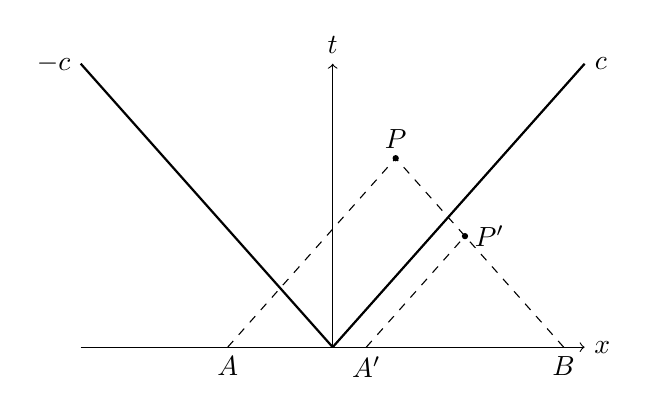
\begin{tikzpicture}[scale=0.8]
  \draw[->] (-4,0) -- (4.,0) node[right] {$x$};
  \draw[->] (0,0) -- (0,4.5) node[above] {$t$};
  \draw[thick] (0,0) -- (4.,4.5) node [right] {$c$};
  \draw[thick] (0,0) -- (-4.,4.5) node [left] {$-c$};
  \fill[black] (1.,3.) circle (0.05) node [above] {$P$};
  \draw[dashed] (1-8./3.,0.) node [below] {$A$}  -- (1.,3.);
  \draw[dashed] (1+8./3.,0.)node [below] {$B$}  -- (1.,3.);
  %% Intersection of positive solid line and negative dashed one
  %\fill[black] (0.5+12/9.,2.) circle (0.05) node [above] {$P'$};
  \fill[black] (2.10,1.762499) circle (0.05) node [right] {$P'$};
  \draw[dashed] (0.5333,0.) node [below] {$A'$}  -- (2.10,1.762499);
\end{tikzpicture}



%%% Local Variables:
%%% mode: latex
%%% TeX-master: "../../mainManuscript"
%%% End:

  \caption{Solution to Riemann problem \eqref{eq:Riemann_problem} for an elastic bar.}
  \label{fig:elasticity_example}
\end{figure}
Integration of characteristic equations \eqref{eq:elast_charac_equation} respectively along $AP$ and $BP$ yields:
\begin{equation}
  \label{eq:elastic_integral_curves}
  \left\lbrace
    \begin{aligned}
      & \rho c \(v_P - v_A \) - \(\sigma_P - \sigma_A \) = 0\\
      -& \rho c \(v_P - v_B \) - \(\sigma_P - \sigma_B \) = 0
    \end{aligned}
    \right.
\end{equation}
which solution is:
\begin{equation}
  \label{eq:elastic_solution_P}
  v_P = \frac{\sigma_B - \sigma_A}{2\rho c} + \frac{v_A+v_B}{2} \quad ; \quad \sigma_P = \rho c\frac{v_B - v_A}{2} + \frac{\sigma_A+\sigma_B}{2}
\end{equation}
On the other hand, the same procedure for point $P'$ leads to the solution:
\begin{equation}
  \label{eq:elastic_solution_Q}
  v_{P'} = \frac{\sigma_B - \sigma_{A'}}{2\rho c} + \frac{v_{A'}+v_B}{2} \quad ; \quad \sigma_{P'} = \rho c\frac{v_B - v_{A'}}{2} + \frac{\sigma_{A'}+\sigma_B}{2}
\end{equation}
With initial data given for the Riemann problem, it appears that $\Qcb_{A'}=\Qcb_{B}$ and hence, $\Qcb_{P'}=\Qcb_{R} \ne \Qcb_{P}$. Let's assume now that points $P$ and $P'$ are still on each side of the right characteristic straight line emanating from the origin but infinitely close to it. It is obvious that the previous results hold and that the a jump discontinuity propagates in the bar with speed $c$. Hence, we are left with the following condition across a discontinuous wave \cite{Toro} that generalizes to all linear Riemann problems:
\begin{definition}
Given a system of hyperbolic conservation laws $\Qcb_t + \Fcb(\Qcb)_x=\vect{0}$ and a discontinuous wave solution of speed $s_i$ associated to the $i$th characteristic field, the \textbf{Rankine-Hugoniot condition} reads:
\begin{equation}
  \label{eq:rankine-hugoniot}
  \saut{ \Fcb} = s_i \saut{ \Qcb}
\end{equation}
where $\saut{\bullet}$ denotes the jump operator across the discontinuity.  
\end{definition}


\textcolor{Red}{For non-linear discontinuities (shocks) the celerity $s_i$ is not known whereas in the linear case $s_i=\lambda_i$. (Then in the non-linear part, says that in that case the celerity of the shock is not known unlike for linear problems)}
\subsection{Non-linear problems}
We now consider a hyperelastic medium made of a Saint-Venant-Kirchhoff material, infinite in directions $\vect{e}_2$ and $\vect{e}_3$, and semi-infinite in direction $\vect{e}_1$ (\textit{i.e. $x_1 \in [0,+\infty[$}). This medium undergoes a load at $x_1=x=0$ in direction $\vect{e}_1$ so that the deformation gradient and the PK1 tensor are respectively:
\begin{align*}
  &\tens{F}=F\vect{e}_1\otimes\vect{e}_1 + \vect{e}_2\otimes\vect{e}_2 + \vect{e}_3\otimes\vect{e}_3 \\
  & \tens{\Pi}=\Pi_{11}\vect{e}_1\otimes\vect{e}_1 + \Pi_{22}\(\vect{e}_2\otimes\vect{e}_2 + \vect{e}_3\otimes\vect{e}_3 \)
\end{align*}
which corresponds to a plane wave solution. Once again, the Riemann problem considered is \eqref{eq:Riemann_problem} in which $\vect{N}=\vect{e}_1$ and:
\begin{equation*}
 \Qcb = \matrice{v \\ F} \quad ; \quad \Fcb = \matrice{-\frac{1}{\rho_0}\Pi_{11} \\ -v}
\end{equation*}
with neglected body forces. Since the tangent modulus and the acoustic tensor of Saint-Venant-Kirchhoff model \eqref{eq:SVK_tangent},\eqref{eq:SVK_acoustic} depend on the deformation gradient, the integration of characteristic equations \eqref{eq:PDEs_ODEs} is simpler with the quasi-linear form: $\Qcb_t + \drond{\Fcb}{\Qcb}\drond{\Qcb}{X_N}=\vect{0}$ which Jacobian matrix is:
\begin{equation}
  \label{eq:quasi_SVK}
  \Jbsf=\drond{\Fcb}{\Qcb}=-\matrice{0 & -\frac{H_{1111}}{\rho_0} \\ 1 & 0}
\end{equation}
The eigenvalues of this system are similar to that of the general case \eqref{eq:left_eigenfields} but the left eigenvectors are different and yield the following characteristic fields:
\begin{equation}
  \label{eq:SVK_charac_fields}
  \lambda_{1,2}=\pm \sqrt{\frac{\lambda+2\mu}{2\rho_0}\(3F^2-1\) } \quad ; \quad \Lcb^p=\[1\:,\:- \lambda_p \] \quad ; \quad \Rcb^p=\matrice{- \lambda_p \\1} 
\end{equation}
The non-linearity of the problem thus appears in characteristic speeds and eigenvectors.
\begin{definition} A characteristic field is said to be \textbf{genuinely non-linear} if
  \begin{equation}
    \label{eq:linearly-degenerate}
    \nablav_\Qc \lambda_i \cdot \Rcb^i \neq \vect{0},\quad \forall \Qcb \in \Rbb^m
  \end{equation}
\end{definition}
\begin{definition}
  A characteristic field is said to be \textbf{linearly degenerate} if it satisfies
  \begin{equation}
    \label{eq:linearly-degenerate}
    \nablav_\Qc \lambda_i \cdot \Rcb^i = \vect{0},\quad \forall \Qcb \in \Rbb^m
  \end{equation}
  where $\nablav_\Ucb (\bullet)$ is the gradient in the \textit{phase plane} $\(\Uc_1,...,\Uc_m \)$. In particular, linear systems for which eigenvalues are constant, admit only linearly degenerate characteristic fields.
\end{definition}

For the Saint-Venant-Kirchhoff material, equations \eqref{eq:SVK_charac_fields} lead to:
\begin{equation*}
  \nablav_\Qc \lambda_p = \matrice{0\\ \frac{3(\lambda+2\mu)F}{2\rho_0\lambda_p} } \quad \Rightarrow \nablav_\Qc \lambda_p \cdot \Rcb^p = \frac{3(\lambda+2\mu)F}{2\rho_0\lambda_p} 
\end{equation*}
with is not zero since $F>0$. The two characteristic fields are hence genuinely non-linear. However one must pay attention to the vanishing of characteristic speeds that can occur for $F=\frac{1}{\sqrt{3}}$. Indeed, we see that strain states for which $F \leq \frac{1}{\sqrt{3}}$ lead to a loss of hyperbolicity of the system for in such cases the eigenvalues of the Jacobian are non longer real.

\subsection{Integral curves}
\subsection{The Rankine-Hugoniot condition}


%%% Local Variables:
%%% mode: latex
%%% TeX-master: "../mainManuscript"
%%% End:



\section{Approximate--State Riemann solvers}
\label{sec:riemann_solvers}
It has been seen in the previous section that the complete solution of a Riemann problem in solid dynamics is possible for simple problems. However, such a solution may become complicated for multi-dimensional problems or for other non-linear problems. 
Numerical methods such as upwind or Godunov-based methods \cite{Leveque} require the solution of many Riemann problems within a discretized medium. When dealing with non-linear problems, the exact solution of those problems may increase drastically the computational cost, making the numerical scheme prohibitive. Moreover, numerical procedures often require only little information about the solution of Riemann problems and do not need the complete resolution. In that context, alternative procedures have been developed in order to take into account the characteristic structure of a hyperbolic system by computing an approximate solution of Riemann problems. Approximate Riemann solvers developed for Computational Fluid Dynamics allow to extract information for either flux functions (\textit{HLL, HLLC, Roe} and \textit{Osher} approximate Riemann solvers \cite{Trangenstein}, \cite{Toro}) or for vectors of conserved quantities (\textit{approximate--state Riemann solver} \cite[Ch.9]{Toro}, \cite[Ch.22]{Leveque}). Some of those have been applied to specific problems in solid mechanics problems such as the Osher approximate solver (see \cite{LEE_FVM} and \cite{Haider_FVM}) or the HLLC approximate solver (see \cite{Ortega_HLLD}) for hyperelasticity . We recall here the formulation of the approximate-state Riemann solver for solid mechanics. The approach is then applied to the non-linear problem of section \ref{sec:SVK_solution}.

\subsection{General ideas}
As in the previous section, we consider the Riemann problem in the space direction $\vect{N}$:
\begin{equation}
  \label{eq:RP_approx}
  \begin{aligned}
  &\Qcb_t + \Jbsf\(\Qcb\) \drond{\Qcb}{X_N} = \vect{0}, \\
  &\left\lbrace 
    \begin{aligned}
      & \Qcb(X_N,t=0) = \Qcb^L \quad \text{if } X_N< 0\\
      & \Qcb(X_N,t=0) = \Qcb^R \quad \text{if } X_N> 0
    \end{aligned}
    \right.
  \end{aligned}
\end{equation}
The approach for developing an approximate-state Riemann solver consists in linearizing the problem \eqref{eq:RP_approx} by approximating $\Jbsf$ in the vicinity of $\Qcb^L$ and $\Qcb^R$ by a constant matrix $\bar{\Jbsf}=\Jbsf\(\Qcb^L,\Qcb^R\)$ \cite[Ch.15]{Leveque}. Note that this approximation is valid for small jumps in initial data (\textit{i.e }$\Qcb^L\approx\Qcb^R$) and that $\bar{\Jbsf}$ must ensure hyperbolicity of the system, namely $\bar{\Jbsf}$ has real eigenvalues and a complete set of independent eigenvectors. The approximate matrix also satisfies the consistency condition:
\begin{equation}
  \label{eq:approx_constistency}
  \bar{\Jbsf}\(\Qcb,\Qcb\)=\Jbsf\(\Qcb\)
\end{equation}

Such a matrix can be defined by using the definition of right eigenvectors and characteristic speeds $\Jbsf \Rbsf = \Rbsf \Cbsf \Rightarrow \Jbsf = \Rbsf \Cbsf \Rbsf^{-1}$ in which left-going (\textit{resp. right-going}) characteristics and associated eigenvectors are assumed to depend on $\Qcb^L$ (\textit{resp. on} $\Qcb^R$) only. Namely, one writes:
\begin{align*}
  &\Rbsf = \matrice{\Rcb^1(\Qcb^L),\cdots,\Rcb^I(\Qcb^L),\Rcb^{I+1}(\Qcb^R),\cdots,\Rcb^m(\Qcb^R)} \\
  &\Cbsf=\matrice{c_1(\Qcb^L) & & & & & \\ & \cdots & & && \\ & &c_I(\Qcb^L) & & &\\ & & &c_{I+1}(\Qcb^R)& & \\ & & & &\cdots &\\ &&&&&c_m(\Qcb^R)} 
\end{align*}
where $c_I(\Qcb)$ and $m$ are the highest negative eigenvalue and the dimension of the Jacobian matrix. 

At last, the linearized Riemann problem thus written enables the determination of every state vectors $\Qcb(x,t)$ by following the procedure described in section \ref{subsec:charac_Linear_problems} for linear problems, recalled here for convenience for a system of dimension $m$:
\begin{equation}
  \label{eq:approx_RS}
  \begin{aligned}
    &  \Qcb^R-\Qcb^L=\sum_{i=1}^{m} \Rcb^i\delta^i \\
    &  \Qcb(x,t) =\Qcb^R -\sum_{i=I+1}^{m} \Rcb^i\delta^i \\
    &  \Qcb(x,t) =\Qcb^L+ \sum_{i=1}^{I} \Rcb^i\delta^i
  \end{aligned}
\end{equation}
where the point ($x,t$) lies in the region bounded by the $I$th and $I+1$th characteristics.

\begin{remark}
  Note that since one can define a complete set of independent eigenvectors of the Jacobian matrix, the matrix $\Rbsf$ is non-singular so that $\bar{\Jbsf}$ can be uniquely determined. Moreover, the linearization proposed amounts to considering a heterogeneous medium where $\Qcb^{L}$ and $\Qcb^R$ act as material parameters.
\end{remark}

\subsection{Application: Hyperelastic plane wave}
We finish this section with an illustration of the approximate Riemann solver by considering the plane wave problem in a Saint-Venant-Kirchhoff of section \ref{sec:SVK_solution}.
Recall that the eigenvalues and right eigenvectors matrices read for that problem:
\begin{equation}
  \label{eq:SVK_matrices}
  \Cbsf = \matrice{-c & 0 \\ 0 & c} \quad ; \quad \Rbsf = \matrice{c & -c\\ 1&1} \:,\quad c=\sqrt{\frac{\lambda + 2\mu}{2\rho_0}(3F^2-1)}
\end{equation}
Hence, the linearized problem is written with:
\begin{equation}
  \label{eq:SVK_matrices_linear}
  \Cbsf = \matrice{-c_L & 0 \\ 0 & c_R} \quad ; \quad \Rbsf = \matrice{c_L & -c_R\\ 1&1}
\end{equation}
In section \ref{subsec:charac_Linear_problems}, the expression of the wave strengths vector $\vect{\delta}$ has been established for general linear systems of dimension $2$ (see equation \eqref{eq:wave_strengths}):
\begin{equation}
  \vect{\delta}=\frac{1}{c_R+c_L}\matrice{c_R \Delta F +\Delta v\\ c_L \Delta F -\Delta v}
\end{equation}
leading to the solution $\Qcb $ between the two discontinuous waves:
\begin{equation}
  \label{eq:SVK_approx_solution}
  \Qcb  = \Qcb^L + \delta^1 \Rcb^1 = \matrice{v_L \\F_L} +\delta^1 \matrice{c_L \\1} \quad \text{or} \quad \Qcb  = \Qcb^R - \delta^2 \Rcb^2 = \matrice{v_R \\F_R} -\delta^2 \matrice{-c_R \\1}
\end{equation}
Substitutions of $\delta^{1,2}$ from second equations in first ones provide straight lines equations in the phase plane ($F,v$):
\begin{equation}
  \label{eq:approx_straight}
  v  = v_L + c_L(F -F_L) \quad ; \quad v  = v_R + c_R(F_R-F )
\end{equation}
\begin{figure}[h!]
  \centering
  {\definecolor{Purple}{RGB}{120,28,129}
\definecolor{Blue}{RGB}{63,96,174}
\definecolor{Duck}{RGB}{83,158,182}
\definecolor{Green}{RGB}{109,179,136}
\definecolor{Yellow}{RGB}{202,184,67}
\definecolor{Orange}{RGB}{231,133,50}
\definecolor{Red}{RGB}{217,33,32}
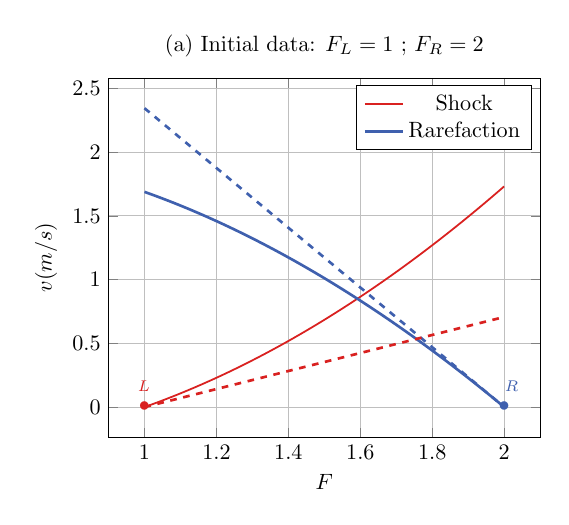
\begin{tikzpicture}[scale=0.8]
\begin{axis}[xlabel=$F$,ylabel=$v (m/s)$,ymajorgrids=true,xmajorgrids=true, title={(a) Initial data: $F_L=1$ ; $F_R=2$}]
  \addplot[Red,thick] coordinates {(1.0,0.0) (1.0196019601960196,0.019889905868838792) (1.0392039203920391,0.04035480171519238) (1.058805880588059,0.06139339246981025) (1.0784078407840785,0.08300445472552491) (1.098009800980098,0.1051868317293367) (1.1176117611761176,0.1279394287977403) (1.1372137213721372,0.1512612091133456) (1.1568156815681567,0.17515118986560513) (1.1764176417641765,0.19960843870261852) (1.196019601960196,0.2246320704646163) (1.2156215621562156,0.25022124417291264) (1.2352235223522352,0.2763751602509047) (1.2548254825482548,0.30309305795616337) (1.2744274427442743,0.330374213004825) (1.2940294029402941,0.3582179353714115) (1.3136313631363137,0.386623567248899) (1.3332333233323332,0.4155904811553686) (1.3528352835283528,0.445118078174895) (1.3724372437243724,0.47520578632153143) (1.3920392039203922,0.5058530590163028) (1.4116411641164117,0.5370593736680643) (1.4312431243124313,0.568824230349938) (1.4508450845084508,0.6011471505637854) (1.4704470447044704,0.6340276760858663) (1.4900490049004902,0.667465367887438) (1.5096509650965095,0.7014598051246006) (1.5292529252925293,0.7360105841921958) (1.5488548854885489,0.7711173178369951) (1.5684568456845684,0.8067796343258441) (1.5880588058805882,0.8429971766647708) (1.6076607660766076,0.8797696018654025) (1.6272627262726274,0.917096580255355) (1.646864686468647,0.9549777948294852) (1.6664666466646665,0.9934129406392047) (1.686068606860686,1.032401724217221) (1.7056705670567056,1.0719438630353144) (1.7252725272527254,1.1120390849929296) (1.7448744874487447,1.1526871279345328) (1.7644764476447645,1.1938877391938512) (1.784078407840784,1.2356406751632294) (1.8036803680368036,1.2779457008865038) (1.8232823282328234,1.320802589673878) (1.8428842884288428,1.3642111227374165) (1.8624862486248626,1.4081710888458763) (1.8820882088208821,1.4526822839976499) (1.9016901690169017,1.4977445111107466) (1.9212921292129215,1.543357579728744) (1.9408940894089408,1.5895213057417645) (1.9604960496049606,1.6362355111215798) (1.9800980098009802,1.6835000236699957) (1.9996999699969997,1.7313146767797576) };
  \addplot[Blue,very thick] coordinates {(1.0,1.6884673989302577) (1.0196019601960196,1.6685781823289632) (1.0392039203920391,1.648117983645035) (1.058805880588059,1.6270917763366024) (1.0784078407840785,1.6055041425368688) (1.098009800980098,1.5833593157699348) (1.1176117611761176,1.5606612177002648) (1.1372137213721372,1.5374134899261505) (1.1568156815681567,1.5136195216278194) (1.1764176417641765,1.48928247372591) (1.196019601960196,1.4644053000848238) (1.2156215621562156,1.4389907661996928) (1.2352235223522352,1.4130414657294894) (1.2548254825482548,1.3865598351776642) (1.2744274427442743,1.3595481669723095) (1.2940294029402941,1.3320086211576845) (1.3136313631363137,1.3039432358761032) (1.3332333233323332,1.2753539367920979) (1.3528352835283528,1.246242545588463) (1.3724372437243724,1.216610787645106) (1.3920392039203922,1.1864602989961286) (1.4116411641164117,1.1557926326474621) (1.4312431243124313,1.12460926432638) (1.4508450845084508,1.092911597724879) (1.4704470447044704,1.0607009692909792) (1.4900490049004902,1.0279786526152188) (1.5096509650965095,0.994745862453826) (1.5292529252925293,0.9610037584250569) (1.5488548854885489,0.9267534484108921) (1.5684568456845684,0.8919959916925568) (1.5880588058805882,0.8567324018451127) (1.6076607660766076,0.8209636494135533) (1.6272627262726274,0.7846906643903794) (1.646864686468647,0.7479143385125069) (1.6664666466646665,0.7106355273934435) (1.686068606860686,0.6728550525050632) (1.7056705670567056,0.6345737030218022) (1.7252725272527254,0.595792237538853) (1.7448744874487447,0.5565113856747698) (1.7644764476447645,0.5167318495678894) (1.784078407840784,0.47645430527509447) (1.8036803680368036,0.43567940408061234) (1.8232823282328234,0.3944077737218566) (1.8428842884288428,0.3526400195386741) (1.8624862486248626,0.31037672555176576) (1.8820882088208821,0.2676184554755838) (1.9016901690169017,0.22436575367049583) (1.9212921292129215,0.18061914603862234) (1.9408940894089408,0.13637914086738703) (1.9604960496049606,0.09164622962443836) (1.9800980098009802,0.04642088770736517) (1.9996999699969997,0.0007035751512764867) };
  \node at (axis cs:1,0) [Red] {$\bullet$};
  \node at (axis cs:2.,0) [Blue] {$\bullet$};
  \node at (axis cs:1,0) [anchor=south,Red] {$\Qcb^L$};
  \node at (axis cs:1.98,0) [above right,Blue] {$\Qcb^R$};
  \addplot[Blue,dashed,very thick,domain=1:2,samples=51,samples y=0]
    ({x},{0.-sqrt(0.5*(12.-1))*(x-2.)});
  \addplot[Red,dashed,very thick,domain=1:2,samples=51,samples y=0]
    ({x},{0.+sqrt(0.5*(2.-1))*(x-1.)});
  \legend{Shock,Rarefaction}
\end{axis}
\end{tikzpicture}
 \phantomsubcaption \label{subfig:SVK_Approx1}}
  {\definecolor{Red}{RGB}{217,33,32}
\definecolor{Blue}{RGB}{63,96,174}
\definecolor{Duck}{RGB}{83,158,182}
\definecolor{Green}{RGB}{109,179,136}
\definecolor{Yellow}{RGB}{202,184,67}
\definecolor{Orange}{RGB}{231,133,50}
\definecolor{Purple}{RGB}{120,28,129}
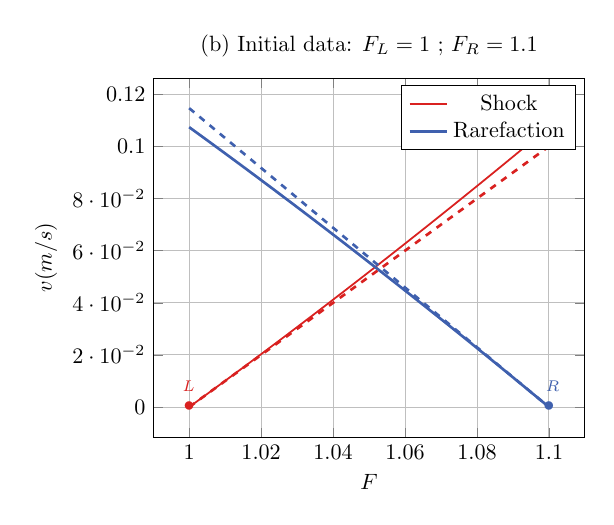
\begin{tikzpicture}[scale=0.8]
\begin{axis}[xlabel=$F$,ylabel=$v (m/s)$,ymajorgrids=true,xmajorgrids=true,title={(b) Initial data: $F_L=1$ ; $F_R=1.1$}]
\addplot[Red,thick] coordinates {(1.0,0.0) (1.001960196019602,0.0019630775609053948) (1.003920392039204,0.003931917267080632) (1.005880588058806,0.005906517718693416) (1.0078407840784078,0.007886877524091035) (1.00980098009801,0.009872995299740863) (1.0117611761176117,0.011864869670167599) (1.0137213721372138,0.01386249926789511) (1.0156815681568157,0.01586588273338493) (1.0176417641764177,0.01787501871497885) (1.0196019601960196,0.019889905868838792) (1.0215621562156216,0.02191054285889049) (1.0235223522352235,0.023936928356764118) (1.0254825482548255,0.025969061041739377) (1.0274427442744274,0.028006939600686957) (1.0294029402940295,0.030050562728014697) (1.0313631363136313,0.03209992912561001) (1.0333233323332334,0.034155037502787186) (1.0352835283528352,0.0362158865762309) (1.0372437243724373,0.03828247506994398) (1.0392039203920391,0.04035480171519238) (1.0411641164116412,0.04243286525045405) (1.0431243124312433,0.044516664421364406) (1.045084508450845,0.04660619798066565) (1.0470447044704472,0.048701464688155255) (1.049004900490049,0.050802463310633685) (1.050965096509651,0.05290919262185532) (1.052925292529253,0.055021651402476585) (1.054885488548855,0.05713983844000798) (1.0568456845684568,0.059263752528762766) (1.058805880588059,0.06139339246981025) (1.0607660766076608,0.06352875707092508) (1.0627262726272628,0.06566984514654145) (1.0646864686468647,0.06781665551770343) (1.0666466646664667,0.06996918701201955) (1.0686068606860686,0.07212743846361445) (1.0705670567056706,0.07429140871308419) (1.0725272527252725,0.07646109660744838) (1.0744874487448746,0.07863650100010654) (1.0764476447644764,0.08081762075079126) (1.0784078407840785,0.08300445472552491) (1.0803680368036805,0.08519700179657394) (1.0823282328232824,0.08739526084240548) (1.0842884288428845,0.08959923074764438) (1.0862486248624863,0.09180891040302837) (1.0882088208820884,0.09402429870536706) (1.0901690169016902,0.09624539455749745) (1.0921292129212923,0.09847219686824406) (1.0940894089408941,0.1007047045523746) (1.0960496049604962,0.10294291653056116) (1.098009800980098,0.1051868317293367) (1.0999699969997,0.10743644908105657) };
\addplot[Blue,very thick] coordinates {(1.0,0.1073874627707086) (1.001960196019602,0.10542438591418365) (1.003920392039204,0.10345555112494406) (1.005880588058806,0.10148096397787983) (1.0078407840784078,0.09950062999930058) (1.00980098009801,0.09751455466754301) (1.0117611761176117,0.09552274341357074) (1.0137213721372138,0.09352520162156171) (1.0156815681568157,0.0915219346294884) (1.0176417641764177,0.089512947729686) (1.0196019601960196,0.08749824616941433) (1.0215621562156216,0.08547783515140679) (1.0235223522352235,0.08345171983441528) (1.0254825482548255,0.08141990533374051) (1.0274427442744274,0.07938239672176006) (1.0294029402940295,0.07733919902844166) (1.0313631363136313,0.0752903172418546) (1.0333233323332334,0.07323575630866758) (1.0352835283528352,0.07117552113464229) (1.0372437243724373,0.06910961658511733) (1.0392039203920391,0.06703804748548585) (1.0411641164116412,0.06496081862166392) (1.0431243124312433,0.06287793474055453) (1.045084508450845,0.06078940055050131) (1.0470447044704472,0.05869522072173673) (1.049004900490049,0.056595399886824015) (1.050965096509651,0.05448994264109064) (1.052925292529253,0.05237885354305752) (1.054885488548855,0.05026213711485809) (1.0568456845684568,0.0481397978426566) (1.058805880588059,0.04601184017705303) (1.0607660766076608,0.04387826853348905) (1.0627262726272628,0.0417390872926421) (1.0646864686468647,0.0395943008008181) (1.0666466646664667,0.037443913370333926) (1.0686068606860686,0.03528792927989956) (1.0705670567056706,0.03312635277498877) (1.0725272527252725,0.03095918806820985) (1.0744874487448746,0.02878643933966615) (1.0764476447644764,0.026608110737315303) (1.0784078407840785,0.0244242063773199) (1.0803680368036805,0.022234730344396287) (1.0823282328232824,0.020039686692156212) (1.0842884288428845,0.017839079443443134) (1.0862486248624863,0.01563291259066641) (1.0882088208820884,0.013421190096127349) (1.0901690169016902,0.011203915892344065) (1.0921292129212923,0.008981093882367926) (1.0940894089408941,0.006752727940100287) (1.0960496049604962,0.00451882191059879) (1.098009800980098,0.0022793796103861676) (1.0999699969997,3.4404827748516585e-05) };
\node at (axis cs:1,0) [Red] {$\bullet$};
  \node at (axis cs:1.1,0) [Blue] {$\bullet$};
  \node at (axis cs:1,0) [anchor=south,Red] {$\Qcb^L$};
  \node at (axis cs:1.097,0) [above right,Blue] {$\Qcb^R$};
  \addplot[Red,dashed,very thick,domain=1:1.1,samples=51,samples y=0]
  ({x},{0.+sqrt(0.5*(3.-1))*(x-1.)});
  \addplot[Blue,dashed,very thick,domain=1:1.1,samples=51,samples y=0]
    ({x},{0.-sqrt(0.5*(3.*(1.1^2)-1))*(x-1.1)});
\legend{Shock,Rarefaction}
\end{axis}
\end{tikzpicture}
 \phantomsubcaption \label{subfig:SVK_Approx4}}
  \caption{Comparison of approximate (dashed lines) and exact (solid lines) solution for a one-dimensional strain problem in a Saint-Venant-Kirchhoff hyperelastic material}
  \label{fig:comparison_exact_approx}
\end{figure}
The intersection of those straight lines in the phase plane corresponds to the approximate solution. Figure \ref{fig:comparison_exact_approx} shows comparisons of approximate and exact solutions for various initial data, all leading to a $1$-shock--$2$-rarefaction exact solution. As expected, approximate and exact solutions are different and get closer for small initial discontinuities, falling in the linearization assumption $\Qcb^L\approx \Qcb^R$. As a consequence, in figures \ref{fig:comparison_exact_approx}\subref{subfig:SVK_Approx1} a big initial discontinuity is considered so that the approximation error is larger than that of figure \ref{fig:comparison_exact_approx}\subref{subfig:SVK_Approx4} for which initial data are based on a weak jump.


%%% Local Variables:
%%% mode: latex
%%% TeX-master: "../mainManuscript"
%%% End:





%%% Local Variables:
%%% mode: latex
%%% TeX-master: "../mainManuscript"
%%% End:


%% Chapter 3: Approximate Riemann solver
%%% MPM "survey"
MPM = collocation method ?
\begin{itemize}
\item \cite{PIC}: Analogy with FVM since mean values of fields are defined in cells
\item \cite{FLIP}: mapping in momentum when particles cross a cell (see \cite{PIC_Nishiguchi}) ; finite volume for each particle (not a dirac) ; Make use of grid velocity and not material point velocity to update particles kinematic by direct interpolation to model \textit{collisional fluids} $\vect{v}_p=S_{ip}\vect{v}_i$
\item \cite{Mass_Flip}: "coarse-grained" (see \cite{Brackbill_PIC}), better to have a \textit{sub-grid-scale motion} and no additional diffusion ; mapp changes of fields instead of fields 
\end{itemize}


%%% Local Variables:
%%% mode: latex
%%% TeX-master: "../mainManuscript"
%%% End:


%% Chapter 4: Extension of the Material Point Method
%\chapter{Numerical Results}
\section*{Introduction}
The Discontinuous Galerkin Material Point Method developed in the previous chapter is now illustrated and compared to other numerical schemes and exact solutions. 
First, problems falling in the small strains framework are considered in section \ref{sec:hpp_simulations}. More specifically, DGMPM solutions of the Riemann problem in an elastic bar is compared MPM to ones in section \ref{subsec:hpp_bar}. The methods are then applied to the solution of problems involving multi-dimensional stress and one-dimensional strain states (plane wave problem) in section \ref{subsec:hpp_planewave}, and to the solution of plane strain problems in sections \ref{subsec:el_planestrain} and \ref{subsec:ep_planestrain}. Comparisons with MPM, FVM, FEM and exact (when existing) solutions are shown for elastic, elastic-viscoplastic and elastoplastic solids.
%one and two-dimensional problems that fall within the infinitesimal theory will be considered for elastic, elastic-viscoplastic and elastoplastic materials in sections \ref{sec:hpp_bar} and \ref{sec:hpp_planewave}.

Second, attention is paid to problems involving waves travelling in finite deforming solids in section \ref{sec:he_simulations}, for which history-dependent constitutive models are not considered.
%For that purpose, the propagation of plane waves in a hyperelastic Saint-Venant-Kirchhoff medium and a plane strain state problem in a Neo-Hookean solid are considered (sections \ref{subsec:he_planewave} and \ref{subsec:he_plate}). The DGMPM simulations performed on the former cases are compared to the MPM solution and the exact one, while comparisons with MPM and FEM are proposed on the latter.
For that purpose, DGMPM simulations performed on plane wave problems in a hyperelastic Saint-Venant-Kirchhoff medium are compared to MPM and exact solutions in section \ref{subsec:he_planewave}. At last, a comparison between DGMPM, FEM and MPM solutions of a plane strain state problem in a Neo-Hookean solid is proposed in section \ref{subsec:he_plate}.

Although several constitutive models are assumed in this chapter, elastic, viscous and plastic properties considered ar the same for every materials. Thus, table \ref{tab:material} summarizes the values of Young's modulus $E$, Poisson ratio $\nu$ and reference mass density $\rho_0$.
In addition, linear isotropic and kinematic hardenings of modulus $H$ and tensile yield stress $\sigma^y$ are assumed for plastic evolutions, along with the viscosity $\eta$ and sensitivity $n$ for viscous ones.
\begin{table}[h!]
  \centering
    \begin{tabular}{l|lN}
    \hline
    $E=2\times 10^{11}\:Pa$ & $\sigma^y=1 \times 10^8 Pa$ & \\ [3pt]
    $\nu=0.3$ & $C=10^{8} Pa$  &\\[3pt]
    $\rho_0 = 7800 \: kg.m^{-3}$ & &\\[3pt]
    \hline
  \end{tabular}

%%% Local Variables:
%%% mode: latex
%%% TeX-master: "../manuscript"
%%% End:

  \caption{Material parameters. The viscosity is expressed as a function of the relaxation time $\tau$.}
  \label{tab:material}
\end{table}
At last, no body forces are considered here.
\section{Linearized geometrical framework}
\label{sec:hpp_simulations}

\subsection{Riemann problem in an isotropic elastic bar}
\label{subsec:hpp_bar}
To begin with, let's focus on the problem that illustrated some shortcomings of the MPM in section \ref{sec:MPM} and motivated the development of the DGMPM.
We thus consider a bar of length $l=6\:m$ in direction $\vect{e}_1$ in which the Cauchy stress and infinitesimal strain tensors are of the form:
\begin{align*}
  & \tens{\sigma} = \sigma \: \vect{e}_1\otimes \vect{e}_1 \\
  & \tens{\eps} = \eps \: \vect{e}_1\otimes \vect{e}_1
\end{align*}
The stress is initially zero everywhere and Riemann-type initial conditions on the axial velocity $v=\vect{v}\cdot\vect{e}_1$ are prescribed: $v=v_0>0$ for $x_1\in [0,L/2[$ and $v=-v_0$ for $x_1\in \:]L/2,L]$. In addition, both ends of the domain are traction free.
%The bar is assumed elastic with density $\rho=7800 \: kg.m^{-3}$, Poisson ration $\nu=0.3$ and Young's modulus $E=2\times 10^{11}\:Pa$.
The exact solution of this problem \cite[Ch.1]{Wang}, recalled in section \ref{subsec:charac_Linear_problems}, consists of two elastic discontinuities propagating leftward and rightward in the bar at constant speeds $c=\pm\sqrt{E/\rho}$. 
The discretization of the domain lies on a regular background grid made of $50$ regular cells containing material points distributed so that two situations are distinguished: each cell contains one particle that coincides with the element centroid for the $1ppc$ discretization; each cell contains two particles symmetrically placed with respect to element centers and regularly spaced in the grid for the $2ppc$ discretization.
% \begin{itemize}
% \item[(1)] $1ppc$ discretization: each cell contains one particle that coincides with the element centroid
% \item[(2)] $2ppc$ discretization: each cell contains two particles symmetrically placed with respect to element centers. The particles are moreover regularly spaced in the grid.
% \end{itemize}
% Those two configurations using either one or two Particles Per Cell are respectively referred to as $1ppc$ and $2ppc$ hereinafter.

The problem is solved on the one hand with the MPM-USL in which the nodal velocity is based on either FLIP of PIC mappings ($CFL=0.5$), and with the DGMPM coupled with both Euler and RK2 time integration on the other hand.
% The Courant number is set at $CFL=1$ for the DGMPM-Euler with 1ppc and DGMPM-RK2 with 2ppc, while it must be reduced to $CFL=0.5$ if 2ppc are used within or the DGMPM-Euler 
%  ($CFL$ satisfying the stability condition \eqref{eq:stability} in section \ref{sec:DGMPM_analysis}).
\begin{figure}[h!]
  \centering
  {\phantomsubcaption \label{subfig:rp_elastic1}}
  {\phantomsubcaption \label{subfig:rp_elastic2}}
  % \begin{tikzpicture}[scale=0.9]
  \begin{groupplot}[group style={group size=2 by 1,
      ylabels at=edge left, yticklabels at=edge left,
      horizontal sep=4.ex,
      vertical sep=2ex,},
    ymajorgrids=true,xmajorgrids=true,
    enlargelimits=0,
    xmin=0.,xmax=6.,
    ylabel=$\sigma (Pa)$,
    xlabel=$x (m)$,
    axis on top,scale only axis,width=0.45\linewidth%,xtick=\empty,ytick=\empty,width=0.25\linewidth,
    ]
    %% FIRST PLOT
    \nextgroupplot[title={(a) time $t = 1.21\times 10^{-4} $ s.}]
    \addplot[Red,very thick,mark=none,dashed,mark size=3pt] coordinates {(0.0,-1.7182156787438973e-08) (0.12244897959183673,4.295539196859743e-08) (0.24489795918367346,1.718215678743897e-08) (0.36734693877551017,8.591078393719486e-09) (0.4897959183673469,-1.7182156787438973e-08) (0.6122448979591837,-3.4364313574877946e-08) (0.7346938775510203,-2.5773235181158458e-08) (0.8571428571428571,0.0) (0.9795918367346939,0.0) (1.1020408163265305,-1.7182156787438973e-08) (1.2244897959183674,1.7182156787438973e-08) (1.346938775510204,0.0) (1.4693877551020407,0.0) (1.5918367346938775,0.0) (1.7142857142857142,0.0) (1.836734693877551,-10490.417480468344) (1.9591836734693877,-180244.44580078288) (2.0816326530612246,-1426887.5122070103) (2.204081632653061,-6905937.1948242355) (2.326530612244898,-22447967.529296968) (2.4489795918367347,-53339385.9863282) (2.571428571428571,-87870025.6347658) (2.693877551020408,-120363616.94335955) (2.816326530612245,-112137222.29003876) (2.9387755102040813,-95318222.04589848) (3.061224489795918,-95318222.04589835) (3.183673469387755,-112137222.29003933) (3.306122448979592,-120363616.94335933) (3.4285714285714284,-87870025.63476545) (3.5510204081632653,-53339385.98632792) (3.673469387755102,-22447967.529296756) (3.7959183673469385,-6905937.194824192) (3.9183673469387754,-1426887.512207019) (4.040816326530612,-180244.44580077427) (4.163265306122449,-10490.417480468344) (4.285714285714286,0.0) (4.408163265306122,0.0) (4.530612244897959,0.0) (4.653061224489796,0.0) (4.775510204081632,1.7182156787438973e-08) (4.8979591836734695,-1.7182156787438973e-08) (5.020408163265306,0.0) (5.142857142857142,0.0) (5.26530612244898,0.0) (5.387755102040816,0.0) (5.5102040816326525,0.0) (5.63265306122449,0.0) (5.755102040816326,0.0) (5.877551020408163,0.0) (6.0,0.0) };
\addplot[Duck,thin,mark=*,solid,mark size=3pt] coordinates {(0.0,8.591078393719486e-09) (0.12244897959183673,7.731970554347537e-08) (0.24489795918367346,9.450186233091434e-08) (0.36734693877551017,2.5773235181158448e-08) (0.4897959183673469,-2.5773235181158458e-08) (0.6122448979591837,-7.731970554347535e-08) (0.7346938775510203,-9.450186233091434e-08) (0.8571428571428571,-5.1546470362316915e-08) (0.9795918367346939,-2.5773235181158458e-08) (1.1020408163265305,-1.7182156787438973e-08) (1.2244897959183674,1.7182156787438973e-08) (1.346938775510204,0.0) (1.4693877551020407,0.0) (1.5918367346938775,0.0) (1.7142857142857142,0.0) (1.836734693877551,-97656.24999999622) (1.9591836734693877,-1074218.75000001) (2.0816326530612246,-5468750.0000000205) (2.204081632653061,-17187500.00000005) (2.326530612244898,-37695312.50000009) (2.4489795918367347,-62304687.500000015) (2.571428571428571,-82812500.00000007) (2.693877551020408,-94531250.00000004) (2.816326530612245,-98925781.24999997) (2.9387755102040813,-99902343.74999999) (3.061224489795918,-99902343.75000001) (3.183673469387755,-98925781.24999999) (3.306122448979592,-94531250.0) (3.4285714285714284,-82812499.99999993) (3.5510204081632653,-62304687.49999988) (3.673469387755102,-37695312.499999896) (3.7959183673469385,-17187499.999999933) (3.9183673469387754,-5468749.99999996) (4.040816326530612,-1074218.7500000014) (4.163265306122449,-97656.24999999622) (4.285714285714286,0.0) (4.408163265306122,0.0) (4.530612244897959,0.0) (4.653061224489796,0.0) (4.775510204081632,1.7182156787438973e-08) (4.8979591836734695,-1.7182156787438973e-08) (5.020408163265306,0.0) (5.142857142857142,0.0) (5.26530612244898,0.0) (5.387755102040816,0.0) (5.5102040816326525,0.0) (5.63265306122449,0.0) (5.755102040816326,0.0) (5.877551020408163,0.0) (6.0,0.0) };
\addplot[Orange,very thick,mark=none,densely dotted,mark size=3pt] coordinates {(0.0,0.0) (0.06060606060606061,0.0) (0.12121212121212122,0.0) (0.18181818181818182,0.0) (0.24242424242424243,0.0) (0.30303030303030304,0.0) (0.36363636363636365,0.0) (0.42424242424242425,0.0) (0.48484848484848486,0.0) (0.5454545454545454,0.0) (0.6060606060606061,8.504299824085957e-09) (0.6666666666666667,8.504299824085957e-09) (0.7272727272727273,-1.7008599648171914e-08) (0.7878787878787878,-1.7008599648171914e-08) (0.8484848484848485,0.0) (0.9090909090909092,0.0) (0.9696969696969697,-2.551289947225787e-08) (1.0303030303030303,-2.551289947225787e-08) (1.0909090909090908,0.0) (1.1515151515151516,0.0) (1.2121212121212122,1.7008599648171914e-08) (1.2727272727272727,1.7008599648171914e-08) (1.3333333333333335,-8.504299824085957e-09) (1.393939393939394,-8.504299824085957e-09) (1.4545454545454546,-8.504299824085957e-09) (1.5151515151515151,-8.504299824085957e-09) (1.5757575757575757,8.504299824085957e-09) (1.6363636363636365,8.504299824085957e-09) (1.696969696969697,1.7008599648171914e-08) (1.7575757575757576,1.7008599648171914e-08) (1.8181818181818183,-5499.273538584786) (1.878787878787879,-5499.273538584786) (1.9393939393939394,-115492.194890958) (2.0,-115492.194890958) (2.0606060606060606,-1086898.8931179084) (2.121212121212121,-1086898.8931179084) (2.1818181818181817,-6038592.01073648) (2.2424242424242427,-6038592.01073648) (2.303030303030303,-21882501.244545024) (2.3636363636363638,-21882501.244545024) (2.4242424242424243,-54484376.31130224) (2.484848484848485,-54484376.31130224) (2.5454545454545454,-94001361.72771455) (2.606060606060606,-94001361.72771455) (2.666666666666667,-117371180.65357204) (2.7272727272727275,-117371180.65357204) (2.787878787878788,-111648218.33372112) (2.8484848484848486,-111648218.33372112) (2.909090909090909,-93365879.35686114) (2.9696969696969697,-93365879.35686114) (3.0303030303030303,-93365879.35686119) (3.090909090909091,-93365879.35686119) (3.1515151515151514,-111648218.33372112) (3.2121212121212124,-111648218.33372112) (3.272727272727273,-117371180.6535721) (3.3333333333333335,-117371180.6535721) (3.393939393939394,-94001361.72771455) (3.4545454545454546,-94001361.72771455) (3.515151515151515,-54484376.3113022) (3.5757575757575757,-54484376.3113022) (3.6363636363636367,-21882501.24454498) (3.6969696969696972,-21882501.24454498) (3.757575757575758,-6038592.01073648) (3.8181818181818183,-6038592.01073648) (3.878787878787879,-1086898.8931178998) (3.9393939393939394,-1086898.8931178998) (4.0,-115492.19489097499) (4.0606060606060606,-115492.19489097499) (4.121212121212121,-5499.273538601796) (4.181818181818182,-5499.273538601796) (4.242424242424242,-8.504299824085957e-09) (4.303030303030303,-8.504299824085957e-09) (4.363636363636363,1.7008599648171914e-08) (4.424242424242425,1.7008599648171914e-08) (4.484848484848485,-8.504299824085957e-09) (4.545454545454546,-8.504299824085957e-09) (4.606060606060606,0.0) (4.666666666666667,0.0) (4.7272727272727275,0.0) (4.787878787878788,0.0) (4.848484848484849,0.0) (4.909090909090909,0.0) (4.96969696969697,0.0) (5.03030303030303,0.0) (5.090909090909091,0.0) (5.151515151515151,0.0) (5.212121212121212,0.0) (5.2727272727272725,0.0) (5.333333333333334,0.0) (5.3939393939393945,0.0) (5.454545454545455,0.0) (5.515151515151516,0.0) (5.575757575757576,0.0) (5.636363636363637,0.0) (5.696969696969697,0.0) (5.757575757575758,0.0) (5.818181818181818,0.0) (5.878787878787879,0.0) (5.9393939393939394,0.0) (6.0,0.0) };
\addplot[Blue,very thick,mark=none,solid,mark size=3pt] coordinates {(0.0,2.205276437763443e-23) (0.12244897959183673,-4.821391029817259e-08) (0.24489795918367346,-3.616043272362948e-08) (0.36734693877551017,2.4106955149086293e-08) (0.4897959183673469,-3.616043272362948e-08) (0.6122448979591837,-2.4106955149086323e-08) (0.7346938775510203,1.2053477574543153e-08) (0.8571428571428571,-1.205347757454316e-08) (0.9795918367346939,1.205347757454315e-08) (1.1020408163265305,1.2053477574543135e-08) (1.2244897959183674,2.4106955149086313e-08) (1.346938775510204,2.41069551490863e-08) (1.4693877551020407,-6.3007898221812655e-24) (1.5918367346938775,-6.3007898221812655e-24) (1.7142857142857142,1.2053477574543152e-08) (1.836734693877551,-2.4106955149086303e-08) (1.9591836734693877,0.0) (2.0816326530612246,0.0) (2.204081632653061,1.5751974555453164e-23) (2.326530612244898,1.5751974555453164e-23) (2.4489795918367347,-99999999.99999999) (2.571428571428571,-100000000.00000003) (2.693877551020408,-100000000.0) (2.816326530612245,-99999999.99999999) (2.9387755102040813,-100000000.0) (3.061224489795918,-99999999.99999997) (3.183673469387755,-100000000.0) (3.306122448979592,-99999999.99999999) (3.4285714285714284,-99999999.99999999) (3.5510204081632653,-99999999.99999999) (3.673469387755102,-1.2601579644362531e-23) (3.7959183673469385,1.2053477574543145e-08) (3.9183673469387754,1.2053477574543147e-08) (4.040816326530612,-3.6160432723629465e-08) (4.163265306122449,1.4176777099907847e-23) (4.285714285714286,-1.4176777099907847e-23) (4.408163265306122,-2.410695514908632e-08) (4.530612244897959,-1.2053477574543148e-08) (4.653061224489796,1.2053477574543138e-08) (4.775510204081632,-1.8902369466543796e-23) (4.8979591836734695,-1.2053477574543148e-08) (5.020408163265306,-2.4106955149086316e-08) (5.142857142857142,3.616043272362944e-08) (5.26530612244898,-1.2053477574543148e-08) (5.387755102040816,-1.8902369466543796e-23) (5.5102040816326525,2.410695514908629e-08) (5.63265306122449,-1.8902369466543796e-23) (5.755102040816326,-1.2053477574543173e-08) (5.877551020408163,2.410695514908629e-08) (6.0,-1.5751974555453164e-23) };
\addplot[Purple,very thick,mark=|,solid,mark size=3pt] coordinates {(0.0,1.1954895665669321e-11) (0.06060606060606061,-1.1954895665669323e-11) (0.12121212121212122,-9.040062200539418e-09) (0.18181818181818182,-1.5066892948546882e-08) (0.24242424242424243,-2.0148953581298875e-08) (0.30303030303030304,-4.011843429141689e-08) (0.36363636363636365,-3.9801572080816714e-08) (0.42424242424242425,-4.457277094098534e-08) (0.48484848484848486,-3.051726216575409e-08) (0.5454545454545454,-2.975012570696168e-08) (0.6060606060606061,-1.895467099939049e-08) (0.6666666666666667,-5.152284149695791e-09) (0.7272727272727273,-1.179037790916254e-08) (0.7878787878787878,-1.2316577239923773e-08) (0.8484848484848485,-2.5473583645144106e-08) (0.9090909090909092,1.3666284960577943e-09) (0.9696969696969697,3.645346560854217e-08) (1.0303030303030303,2.381392226417357e-08) (1.0909090909090908,2.4282772581015557e-08) (1.1515151515151516,2.3931137717157056e-08) (1.2121212121212122,1.2243410979431472e-08) (1.2727272727272727,1.1863544169654833e-08) (1.3333333333333335,1.2583171413268185e-08) (1.393939393939394,1.1523783735818112e-08) (1.4545454545454546,2.7371193430229355e-08) (1.5151515151515151,2.0842716867943245e-08) (1.5757575757575757,9.624966966074275e-09) (1.6363636363636365,1.448198818301203e-08) (1.696969696969697,2.104809967646104e-08) (1.7575757575757576,1.511233304716842e-08) (1.8181818181818183,-3666.244447226061) (1.878787878787879,-10998.733341690284) (1.9393939393939394,-100618.04205178331) (2.0,-262747.51871824573) (2.0606060606060606,-1140066.2362575496) (2.121212121212121,-2551162.9879474747) (2.1818181818181817,-6952185.183763518) (2.2424242424242427,-13110550.493001966) (2.303030303030303,-25132333.114743244) (2.3636363636363638,-39370855.31651974) (2.4242424242424243,-56894854.8287153) (2.484848484848485,-73865127.93600555) (2.5454545454545454,-86159824.57995412) (2.606060606060606,-95498106.62865634) (2.666666666666667,-98513982.44500154) (2.7272727272727275,-100261419.26646227) (2.787878787878788,-100094961.18873355) (2.8484848484848486,-100070640.63102004) (2.909090909090909,-100007508.13633199) (2.9696969696969697,-99998390.4883265) (3.0303030303030303,-99998390.48832652) (3.090909090909091,-100007508.136332) (3.1515151515151514,-100070640.63102002) (3.2121212121212124,-100094961.18873355) (3.272727272727273,-100261419.2664623) (3.3333333333333335,-98513982.44500159) (3.393939393939394,-95498106.62865636) (3.4545454545454546,-86159824.57995415) (3.515151515151515,-73865127.93600555) (3.5757575757575757,-56894854.8287153) (3.6363636363636367,-39370855.31651971) (3.6969696969696972,-25132333.11474323) (3.757575757575758,-13110550.493001949) (3.8181818181818183,-6952185.183763516) (3.878787878787879,-2551162.987947458) (3.9393939393939394,-1140066.2362575415) (4.0,-262747.51871824026) (4.0606060606060606,-100618.04205180079) (4.121212121212121,-10998.73334169629) (4.181818181818182,-3666.2444472321054) (4.242424242424242,6.026554865799796e-09) (4.303030303030303,6.026922708743356e-09) (4.363636363636363,2.0086063933044116e-09) (4.424242424242425,-1.4062083967847561e-08) (4.484848484848485,0.0) (4.545454545454546,0.0) (4.606060606060606,0.0) (4.666666666666667,0.0) (4.7272727272727275,0.0) (4.787878787878788,0.0) (4.848484848484849,0.0) (4.909090909090909,0.0) (4.96969696969697,0.0) (5.03030303030303,0.0) (5.090909090909091,0.0) (5.151515151515151,0.0) (5.212121212121212,0.0) (5.2727272727272725,0.0) (5.333333333333334,0.0) (5.3939393939393945,0.0) (5.454545454545455,0.0) (5.515151515151516,0.0) (5.575757575757576,0.0) (5.636363636363637,0.0) (5.696969696969697,0.0) (5.757575757575758,0.0) (5.818181818181818,0.0) (5.878787878787879,0.0) (5.9393939393939394,-6.0267272921795895e-09) (6.0,-6.026750282363563e-09) };
\addplot[Green,thick,mark=x,only marks,mark size=3pt] coordinates {(0.0,-2.1093585755450518e-08) (0.06060606060606061,-3.0133693936357875e-09) (0.12121212121212122,-2.504863308459749e-08) (0.18181818181818182,-2.316527721357512e-08) (0.24242424242424243,-1.40780851358922e-08) (0.30303030303030304,-1.0028870013194108e-08) (0.36363636363636365,-4.3717398156106705e-08) (0.42424242424242425,-2.8603467291152215e-08) (0.48484848484848486,7.156752309884969e-09) (0.5454545454545454,1.6950202839201318e-08) (0.6060606060606061,-4.3693856207718916e-08) (0.6666666666666667,-5.2733964388626276e-08) (0.7272727272727273,3.3523734504198126e-08) (0.7878787878787878,3.87971309430608e-08) (0.8484848484848485,-1.4878511381076717e-08) (0.9090909090909092,-9.228443768009598e-09) (0.9696969696969697,5.57002498854865e-08) (1.0303030303030303,8.894148100903133e-08) (1.0909090909090908,-5.925508409204129e-08) (1.1515151515151516,-3.7172736504303915e-08) (1.2121212121212122,2.895659651696907e-09) (1.2727272727272727,2.1211295497389412e-08) (1.3333333333333335,3.926796991081633e-08) (1.393939393939394,8.945940387356272e-09) (1.4545454545454546,-2.0104823923163776e-08) (1.5151515151515151,-2.810908637500884e-08) (1.5757575757575757,5.155686696923746e-09) (1.6363636363636365,-5.155686696923745e-09) (1.696969696969697,1.909252014248924e-08) (1.7575757575757576,5.014435006597071e-09) (1.8181818181818183,-1.0546792877725262e-08) (1.878787878787879,-1.3560162271361046e-08) (1.9393939393939394,-4.8967252646581575e-09) (2.0,-1.9210229884428146e-08) (2.0606060606060606,6.191532425986014e-09) (2.121212121212121,-6.191532425986031e-09) (2.1818181818181817,-1.7774171032773557e-08) (2.2424242424242427,-3.043973926539904e-08) (2.303030303030303,1.7609377394059133e-08) (2.3636363636363638,6.4975777550271785e-09) (2.4242424242424243,-99999999.99999994) (2.484848484848485,-100000000.00000006) (2.5454545454545454,-99999999.99999997) (2.606060606060606,-99999999.99999996) (2.666666666666667,-99999999.99999994) (2.7272727272727275,-99999999.99999994) (2.787878787878788,-100000000.00000001) (2.8484848484848486,-100000000.00000001) (2.909090909090909,-99999999.99999997) (2.9696969696969697,-99999999.99999999) (3.0303030303030303,-99999999.99999996) (3.090909090909091,-99999999.99999997) (3.1515151515151514,-99999999.99999996) (3.2121212121212124,-99999999.99999997) (3.272727272727273,-99999999.99999996) (3.3333333333333335,-99999999.99999999) (3.393939393939394,-99999999.99999999) (3.4545454545454546,-100000000.0) (3.515151515151515,-99999999.99999993) (3.5757575757575757,-100000000.00000009) (3.6363636363636367,0.0) (3.6969696969696972,0.0) (3.757575757575758,0.0) (3.8181818181818183,0.0) (3.878787878787879,0.0) (3.9393939393939394,0.0) (4.0,-6.026738787271577e-09) (4.0606060606060606,-1.8080216361814732e-08) (4.121212121212121,1.8080216361814716e-08) (4.181818181818182,6.0267387872715865e-09) (4.242424242424242,-1.6479363871445125e-10) (4.303030303030303,-2.3942161510371846e-08) (4.363636363636363,2.2105889536125074e-08) (4.424242424242425,2.610802076204755e-08) (4.484848484848485,-1.101763184548084e-08) (4.545454545454546,-1.308932330360547e-08) (4.606060606060606,2.4106955149086287e-08) (4.666666666666667,2.4106955149086323e-08) (4.7272727272727275,-2.4106955149086296e-08) (4.787878787878788,-2.410695514908632e-08) (4.848484848484849,0.0) (4.909090909090909,0.0) (4.96969696969697,0.0) (5.03030303030303,0.0) (5.090909090909091,0.0) (5.151515151515151,0.0) (5.212121212121212,0.0) (5.2727272727272725,0.0) (5.333333333333334,0.0) (5.3939393939393945,0.0) (5.454545454545455,0.0) (5.515151515151516,0.0) (5.575757575757576,0.0) (5.636363636363637,0.0) (5.696969696969697,0.0) (5.757575757575758,0.0) (5.818181818181818,0.0) (5.878787878787879,0.0) (5.9393939393939394,0.0) (6.0,0.0) };
\addplot[black,thin,mark=none,solid,mark size=3pt] coordinates {(0.0,-0.0) (0.12244897959183673,-0.0) (0.24489795918367346,-0.0) (0.36734693877551017,-0.0) (0.4897959183673469,-0.0) (0.6122448979591837,-0.0) (0.7346938775510203,-0.0) (0.8571428571428571,-0.0) (0.9795918367346939,-0.0) (1.1020408163265305,-0.0) (1.2244897959183674,-0.0) (1.346938775510204,-0.0) (1.4693877551020407,-0.0) (1.5918367346938775,-0.0) (1.7142857142857142,-0.0) (1.836734693877551,-0.0) (1.9591836734693877,-0.0) (2.0816326530612246,-0.0) (2.204081632653061,-0.0) (2.326530612244898,-0.0) (2.4489795918367347,-100000000.0) (2.571428571428571,-100000000.0) (2.693877551020408,-100000000.0) (2.816326530612245,-100000000.0) (2.9387755102040813,-100000000.0) (3.061224489795918,-100000000.0) (3.183673469387755,-100000000.0) (3.306122448979592,-100000000.0) (3.4285714285714284,-100000000.0) (3.5510204081632653,-100000000.0) (3.673469387755102,-0.0) (3.7959183673469385,-0.0) (3.9183673469387754,-0.0) (4.040816326530612,-0.0) (4.163265306122449,-0.0) (4.285714285714286,-0.0) (4.408163265306122,-0.0) (4.530612244897959,-0.0) (4.653061224489796,-0.0) (4.775510204081632,-0.0) (4.8979591836734695,-0.0) (5.020408163265306,-0.0) (5.142857142857142,-0.0) (5.26530612244898,-0.0) (5.387755102040816,-0.0) (5.5102040816326525,-0.0) (5.63265306122449,-0.0) (5.755102040816326,-0.0) (5.877551020408163,-0.0) (6.0,-0.0) };
    %% SECOND PLOT
    \nextgroupplot[title={(b) time $t = 4.84\times 10^{-4} $ s.},legend style={at={($(0.62,-0.35)+(0.9cm,1cm)$)},legend columns=4}]
    \addplot[Red,very thick,mark=none,dashed,mark size=3pt] coordinates {(0.0,-745947.6317356245) (0.12244897959183673,-2825505.704681147) (0.24489795918367346,-6801870.379054734) (0.36734693877551017,-14249320.469123462) (0.4897959183673469,-26743878.38137685) (0.6122448979591837,-45064188.07482756) (0.7346938775510203,-68064481.52123177) (0.8571428571428571,-91948308.59367745) (0.9795918367346939,-110948018.79598898) (1.1020408163265305,-119819288.51732583) (1.2244897959183674,-117150564.11810811) (1.346938775510204,-106891678.01826178) (1.4693877551020407,-96652794.70257169) (1.5918367346938775,-92267743.75879696) (1.7142857142857142,-95070577.34692116) (1.836734693877551,-99847820.1972167) (1.9591836734693877,-103232485.94759263) (2.0816326530612246,-101626491.39890483) (2.204081632653061,-100355242.65368447) (2.326530612244898,-98244216.75952996) (2.4489795918367347,-100067772.41751443) (2.571428571428571,-99702418.44172558) (2.693877551020408,-100893884.04862353) (2.816326530612245,-99751345.3825965) (2.9387755102040813,-99889896.90888087) (3.061224489795918,-99889896.90888077) (3.183673469387755,-99751345.38259669) (3.306122448979592,-100893884.04862344) (3.4285714285714284,-99702418.44172575) (3.5510204081632653,-100067772.41751438) (3.673469387755102,-98244216.75953004) (3.7959183673469385,-100355242.65368438) (3.9183673469387754,-101626491.39890482) (4.040816326530612,-103232485.94759259) (4.163265306122449,-99847820.1972167) (4.285714285714286,-95070577.34692109) (4.408163265306122,-92267743.7587969) (4.530612244897959,-96652794.70257166) (4.653061224489796,-106891678.01826191) (4.775510204081632,-117150564.11810826) (4.8979591836734695,-119819288.51732588) (5.020408163265306,-110948018.79598887) (5.142857142857142,-91948308.59367728) (5.26530612244898,-68064481.52123177) (5.387755102040816,-45064188.074827455) (5.5102040816326525,-26743878.38137681) (5.63265306122449,-14249320.469123438) (5.755102040816326,-6801870.379054725) (5.877551020408163,-2825505.7046811893) (6.0,-745947.6317356417) };
\addplot[Duck,thin,mark=*,solid,mark size=3pt] coordinates {(0.0,-3658473.820541984) (0.12244897959183673,-11485497.138528435) (0.24489795918367346,-20650075.223420583) (0.36734693877551017,-31470071.326657515) (0.4897959183673469,-43620393.930359595) (0.6122448979591837,-56234556.96822935) (0.7346938775510203,-68199491.57707022) (0.8571428571428571,-78518360.75669788) (0.9795918367346939,-86590219.21803293) (1.1020408163265305,-92306933.66125712) (1.2244897959183674,-95965467.32727806) (1.346938775510204,-98076133.61253974) (1.4693877551020407,-99170549.7565818) (1.5918367346938775,-99678671.19148654) (1.7142857142857142,-99888928.31124762) (1.836734693877551,-99966022.58725037) (1.9591836734693877,-99990891.70851223) (2.0816326530612246,-99997886.14886712) (2.204081632653061,-99999581.77077132) (2.326530612244898,-99999930.86939865) (2.4489795918367347,-99999990.71487762) (2.571428571428571,-99999999.0267497) (2.693877551020408,-99999999.92533047) (2.816326530612245,-99999999.99627104) (2.9387755102040813,-99999999.99990901) (3.061224489795918,-99999999.99990901) (3.183673469387755,-99999999.99627106) (3.306122448979592,-99999999.9253305) (3.4285714285714284,-99999999.02674973) (3.5510204081632653,-99999990.71487764) (3.673469387755102,-99999930.86939867) (3.7959183673469385,-99999581.77077134) (3.9183673469387754,-99997886.14886712) (4.040816326530612,-99990891.70851222) (4.163265306122449,-99966022.58725034) (4.285714285714286,-99888928.31124759) (4.408163265306122,-99678671.19148651) (4.530612244897959,-99170549.75658175) (4.653061224489796,-98076133.61253972) (4.775510204081632,-95965467.32727805) (4.8979591836734695,-92306933.66125712) (5.020408163265306,-86590219.21803287) (5.142857142857142,-78518360.7566978) (5.26530612244898,-68199491.5770702) (5.387755102040816,-56234556.968229264) (5.5102040816326525,-43620393.930359535) (5.63265306122449,-31470071.32665747) (5.755102040816326,-20650075.223420557) (5.877551020408163,-11485497.138528453) (6.0,-3658473.8205419495) };
\addplot[Orange,very thick,mark=none,densely dotted,mark size=3pt] coordinates {(0.0,-569245.6271305095) (0.06060606060606061,-569245.6271305095) (0.12121212121212122,-2277785.4230159773) (0.18181818181818182,-2277785.4230159773) (0.24242424242424243,-5901161.70250096) (0.30303030303030304,-5901161.70250096) (0.36363636363636365,-13233001.909618562) (0.42424242424242425,-13233001.909618562) (0.48484848484848486,-26238300.23104623) (0.5454545454545454,-26238300.23104623) (0.6060606060606061,-45981632.22002476) (0.6666666666666667,-45981632.22002476) (0.7272727272727273,-70997511.41827326) (0.7878787878787878,-70997511.41827326) (0.8484848484848485,-96258666.79270092) (0.9090909090909092,-96258666.79270092) (0.9696969696969697,-114407544.96327573) (1.0303030303030303,-114407544.96327573) (1.0909090909090908,-119769201.2337222) (1.1515151515151516,-119769201.2337222) (1.2121212121212122,-112838974.87666531) (1.2727272727272727,-112838974.87666531) (1.3333333333333335,-100993168.67842056) (1.393939393939394,-100993168.67842056) (1.4545454545454546,-93414330.53328812) (1.5151515151515151,-93414330.53328812) (1.5757575757575757,-93992004.01740366) (1.6363636363636365,-93992004.01740366) (1.696969696969697,-99087098.74325639) (1.7575757575757576,-99087098.74325639) (1.8181818181818183,-102489655.2966868) (1.878787878787879,-102489655.2966868) (1.9393939393939394,-101890791.3937958) (2.0,-101890791.3937958) (2.0606060606060606,-99782074.12880751) (2.121212121212121,-99782074.12880751) (2.1818181818181817,-99055570.19076754) (2.2424242424242427,-99055570.19076754) (2.303030303030303,-99748095.76886229) (2.3636363636363638,-99748095.76886229) (2.4242424242424243,-100313223.73164806) (2.484848484848485,-100313223.73164806) (2.5454545454545454,-100175907.04998955) (2.606060606060606,-100175907.04998955) (2.666666666666667,-99908114.85126807) (2.7272727272727275,-99908114.85126807) (2.787878787878788,-99919571.77694954) (2.8484848484848486,-99919571.77694954) (2.909090909090909,-100047873.551725) (2.9696969696969697,-100047873.551725) (3.0303030303030303,-100047873.55172497) (3.090909090909091,-100047873.55172497) (3.1515151515151514,-99919571.7769495) (3.2121212121212124,-99919571.7769495) (3.272727272727273,-99908114.851268) (3.3333333333333335,-99908114.851268) (3.393939393939394,-100175907.0499895) (3.4545454545454546,-100175907.0499895) (3.515151515151515,-100313223.73164806) (3.5757575757575757,-100313223.73164806) (3.6363636363636367,-99748095.7688623) (3.6969696969696972,-99748095.7688623) (3.757575757575758,-99055570.19076759) (3.8181818181818183,-99055570.19076759) (3.878787878787879,-99782074.12880753) (3.9393939393939394,-99782074.12880753) (4.0,-101890791.39379583) (4.0606060606060606,-101890791.39379583) (4.121212121212121,-102489655.29668684) (4.181818181818182,-102489655.29668684) (4.242424242424242,-99087098.74325638) (4.303030303030303,-99087098.74325638) (4.363636363636363,-93992004.01740365) (4.424242424242425,-93992004.01740365) (4.484848484848485,-93414330.53328809) (4.545454545454546,-93414330.53328809) (4.606060606060606,-100993168.67842054) (4.666666666666667,-100993168.67842054) (4.7272727272727275,-112838974.87666531) (4.787878787878788,-112838974.87666531) (4.848484848484849,-119769201.2337222) (4.909090909090909,-119769201.2337222) (4.96969696969697,-114407544.96327575) (5.03030303030303,-114407544.96327575) (5.090909090909091,-96258666.79270092) (5.151515151515151,-96258666.79270092) (5.212121212121212,-70997511.41827326) (5.2727272727272725,-70997511.41827326) (5.333333333333334,-45981632.22002478) (5.3939393939393945,-45981632.22002478) (5.454545454545455,-26238300.23104622) (5.515151515151516,-26238300.23104622) (5.575757575757576,-13233001.90961853) (5.636363636363637,-13233001.90961853) (5.696969696969697,-5901161.702500943) (5.757575757575758,-5901161.702500943) (5.818181818181818,-2277785.4230159433) (5.878787878787879,-2277785.4230159433) (5.9393939393939394,-569245.627130518) (6.0,-569245.627130518) };
\addplot[Blue,very thick,mark=none,solid,mark size=3pt] coordinates {(0.0,6.026738787271584e-08) (0.12244897959183673,-1.2053477574543037e-08) (0.24489795918367346,2.410695514908625e-08) (0.36734693877551017,2.4106955149086283e-08) (0.4897959183673469,6.026738787271564e-08) (0.6122448979591837,-99999999.99999984) (0.7346938775510203,-100000000.00000025) (0.8571428571428571,-99999999.9999998) (0.9795918367346939,-100000000.00000009) (1.1020408163265305,-99999999.99999985) (1.2244897959183674,-100000000.0) (1.346938775510204,-99999999.99999991) (1.4693877551020407,-100000000.0) (1.5918367346938775,-99999999.99999979) (1.7142857142857142,-100000000.00000003) (1.836734693877551,-99999999.99999988) (1.9591836734693877,-99999999.99999994) (2.0816326530612246,-99999999.99999994) (2.204081632653061,-99999999.99999999) (2.326530612244898,-99999999.99999991) (2.4489795918367347,-99999999.99999991) (2.571428571428571,-99999999.99999997) (2.693877551020408,-99999999.99999991) (2.816326530612245,-99999999.99999994) (2.9387755102040813,-99999999.99999997) (3.061224489795918,-99999999.99999988) (3.183673469387755,-99999999.99999997) (3.306122448979592,-99999999.99999988) (3.4285714285714284,-100000000.00000003) (3.5510204081632653,-99999999.99999991) (3.673469387755102,-100000000.0) (3.7959183673469385,-100000000.00000003) (3.9183673469387754,-99999999.99999987) (4.040816326530612,-99999999.99999997) (4.163265306122449,-99999999.99999994) (4.285714285714286,-99999999.99999997) (4.408163265306122,-99999999.99999997) (4.530612244897959,-100000000.00000009) (4.653061224489796,-99999999.99999988) (4.775510204081632,-100000000.00000013) (4.8979591836734695,-99999999.99999987) (5.020408163265306,-100000000.00000012) (5.142857142857142,-99999999.99999991) (5.26530612244898,-100000000.00000007) (5.387755102040816,-99999999.99999999) (5.5102040816326525,-2.410695514908632e-08) (5.63265306122449,2.410695514908628e-08) (5.755102040816326,-7.232086544725893e-08) (5.877551020408163,-1.205347757454315e-08) (6.0,-2.4106955149086326e-08) };
\addplot[Purple,very thick,mark=|,solid,mark size=3pt] coordinates {(0.0,-901250.8727450209) (0.06060606060606061,-2481132.001666541) (0.12121212121212122,-4826425.776536643) (0.18181818181818182,-7379655.632326556) (0.24242424242424243,-11256070.988140773) (0.30303030303030304,-15619284.087205578) (0.36363636363636365,-21632650.461414523) (0.42424242424242425,-28194347.738026302) (0.48484848484848486,-36184793.045001954) (0.5454545454545454,-44512745.90296996) (0.6060606060606061,-53388027.81990887) (0.6666666666666667,-62184684.90343942) (0.7272727272727273,-70312839.86926234) (0.7878787878787878,-77956322.11918701) (0.8484848484848485,-83999795.65014975) (0.9090909090909092,-89383013.54381928) (0.9696969696969697,-92952697.00923085) (1.0303030303030303,-95962268.87367085) (1.0909090909090908,-97581224.04592441) (1.1515151515151516,-98874662.75556055) (1.2121212121212122,-99404486.29729274) (1.2727272727272727,-99808341.57283215) (1.3333333333333335,-99915762.38856114) (1.393939393939394,-99996248.63365263) (1.4545454545454546,-100001427.378495) (1.5151515151515151,-100006998.37736051) (1.5757575757575757,-100003237.88768458) (1.6363636363636365,-100001492.41546689) (1.696969696969697,-100000520.10664989) (1.7575757575757576,-100000028.36063254) (1.8181818181818183,-99999995.05295742) (1.878787878787879,-99999970.09524688) (1.9393939393939394,-99999990.32856694) (2.0,-99999997.18169779) (2.0606060606060606,-99999999.42352416) (2.121212121212121,-100000000.25132437) (2.1818181818181817,-100000000.07258461) (2.2424242424242427,-100000000.03564933) (2.303030303030303,-100000000.00601049) (2.3636363636363638,-99999999.99877489) (2.4242424242424243,-99999999.99971391) (2.484848484848485,-99999999.99982226) (2.5454545454545454,-99999999.99998015) (2.606060606060606,-100000000.00000417) (2.666666666666667,-100000000.00000048) (2.7272727272727275,-100000000.0000002) (2.787878787878788,-99999999.99999994) (2.8484848484848486,-99999999.99999994) (2.909090909090909,-99999999.99999994) (2.9696969696969697,-99999999.99999994) (3.0303030303030303,-99999999.99999994) (3.090909090909091,-99999999.99999994) (3.1515151515151514,-99999999.99999996) (3.2121212121212124,-99999999.99999997) (3.272727272727273,-100000000.00000024) (3.3333333333333335,-100000000.00000054) (3.393939393939394,-100000000.0000042) (3.4545454545454546,-99999999.99998017) (3.515151515151515,-99999999.99982227) (3.5757575757575757,-99999999.99971391) (3.6363636363636367,-99999999.99877487) (3.6969696969696972,-100000000.00601052) (3.757575757575758,-100000000.03564937) (3.8181818181818183,-100000000.07258466) (3.878787878787879,-100000000.2513244) (3.9393939393939394,-99999999.42352419) (4.0,-99999997.18169783) (4.0606060606060606,-99999990.328567) (4.121212121212121,-99999970.09524693) (4.181818181818182,-99999995.05295746) (4.242424242424242,-100000028.36063258) (4.303030303030303,-100000520.10664994) (4.363636363636363,-100001492.41546696) (4.424242424242425,-100003237.88768464) (4.484848484848485,-100006998.37736058) (4.545454545454546,-100001427.37849504) (4.606060606060606,-99996248.63365267) (4.666666666666667,-99915762.38856122) (4.7272727272727275,-99808341.57283223) (4.787878787878788,-99404486.29729284) (4.848484848484849,-98874662.75556065) (4.909090909090909,-97581224.04592451) (4.96969696969697,-95962268.87367095) (5.03030303030303,-92952697.00923099) (5.090909090909091,-89383013.5438194) (5.151515151515151,-83999795.65014987) (5.212121212121212,-77956322.11918712) (5.2727272727272725,-70312839.86926243) (5.333333333333334,-62184684.90343948) (5.3939393939393945,-53388027.81990896) (5.454545454545455,-44512745.90297001) (5.515151515151516,-36184793.04500202) (5.575757575757576,-28194347.73802632) (5.636363636363637,-21632650.461414546) (5.696969696969697,-15619284.087205617) (5.757575757575758,-11256070.988140827) (5.818181818181818,-7379655.632326601) (5.878787878787879,-4826425.7765366705) (5.9393939393939394,-2481132.001666579) (6.0,-901250.8727450437) };
\addplot[Green,thick,mark=x,only marks,mark size=3pt] coordinates {(0.0,-6.52473551238276e-08) (0.06060606060606061,-5.528742062160391e-08) (0.12121212121212122,-5.4360491549496524e-08) (0.18181818181818182,-4.206732904684871e-08) (0.24242424242424243,2.6389399231237735e-10) (0.30303030303030304,2.3843061156773917e-08) (0.36363636363636365,1.6444762021031894e-08) (0.42424242424242425,7.662193128054401e-09) (0.48484848484848486,-2.6065356036709213e-08) (0.5454545454545454,-4.625550941054968e-08) (0.6060606060606061,-99999999.99999985) (0.6666666666666667,-99999999.99999993) (0.7272727272727273,-99999999.99999994) (0.7878787878787878,-99999999.99999994) (0.8484848484848485,-99999999.99999994) (0.9090909090909092,-99999999.99999994) (0.9696969696969697,-100000000.0) (1.0303030303030303,-100000000.0) (1.0909090909090908,-99999999.99999988) (1.1515151515151516,-99999999.9999999) (1.2121212121212122,-99999999.99999991) (1.2727272727272727,-99999999.99999993) (1.3333333333333335,-99999999.99999996) (1.393939393939394,-99999999.99999997) (1.4545454545454546,-99999999.99999988) (1.5151515151515151,-99999999.99999988) (1.5757575757575757,-99999999.99999991) (1.6363636363636365,-99999999.99999993) (1.696969696969697,-99999999.99999997) (1.7575757575757576,-99999999.99999999) (1.8181818181818183,-99999999.99999994) (1.878787878787879,-99999999.99999994) (1.9393939393939394,-99999999.99999994) (2.0,-99999999.99999994) (2.0606060606060606,-99999999.99999996) (2.121212121212121,-99999999.99999999) (2.1818181818181817,-99999999.99999996) (2.2424242424242427,-99999999.99999997) (2.303030303030303,-99999999.99999994) (2.3636363636363638,-99999999.99999994) (2.4242424242424243,-99999999.99999994) (2.484848484848485,-99999999.99999994) (2.5454545454545454,-99999999.9999999) (2.606060606060606,-99999999.99999993) (2.666666666666667,-99999999.99999994) (2.7272727272727275,-99999999.99999994) (2.787878787878788,-99999999.99999996) (2.8484848484848486,-99999999.99999999) (2.909090909090909,-99999999.99999991) (2.9696969696969697,-99999999.99999993) (3.0303030303030303,-99999999.99999994) (3.090909090909091,-99999999.99999994) (3.1515151515151514,-99999999.99999994) (3.2121212121212124,-99999999.99999994) (3.272727272727273,-100000000.0) (3.3333333333333335,-100000000.0) (3.393939393939394,-99999999.99999991) (3.4545454545454546,-99999999.99999993) (3.515151515151515,-99999999.99999999) (3.5757575757575757,-100000000.0) (3.6363636363636367,-99999999.99999991) (3.6969696969696972,-99999999.99999993) (3.757575757575758,-99999999.99999993) (3.8181818181818183,-99999999.99999994) (3.878787878787879,-100000000.00000004) (3.9393939393939394,-100000000.00000003) (4.0,-99999999.99999991) (4.0606060606060606,-99999999.99999991) (4.121212121212121,-100000000.00000001) (4.181818181818182,-100000000.00000003) (4.242424242424242,-99999999.99999993) (4.303030303030303,-99999999.99999994) (4.363636363636363,-99999999.99999997) (4.424242424242425,-99999999.99999997) (4.484848484848485,-100000000.00000006) (4.545454545454546,-100000000.00000006) (4.606060606060606,-99999999.99999991) (4.666666666666667,-99999999.99999993) (4.7272727272727275,-99999999.99999996) (4.787878787878788,-99999999.99999997) (4.848484848484849,-99999999.99999996) (4.909090909090909,-99999999.99999999) (4.96969696969697,-99999999.99999997) (5.03030303030303,-99999999.99999996) (5.090909090909091,-99999999.99999997) (5.151515151515151,-99999999.99999999) (5.212121212121212,-99999999.99999996) (5.2727272727272725,-99999999.99999997) (5.333333333333334,-99999999.99999991) (5.3939393939393945,-100000000.00000009) (5.454545454545455,-6.171875818689624e-09) (5.515151515151516,6.171875818689572e-09) (5.575757575757576,-3.413288241873195e-08) (5.636363636363637,-6.229493817761331e-08) (5.696969696969697,2.564453865316311e-08) (5.757575757575758,-1.5375835040768292e-09) (5.818181818181818,-5.420092204753976e-08) (5.878787878787879,-4.222689854880543e-08) (5.9393939393939394,3.843223074305013e-09) (6.0,-3.8432230743049925e-09) };
\addplot[black,thin,mark=none,solid,mark size=3pt] coordinates {(0.0,-0.0) (0.12244897959183673,-0.0) (0.24489795918367346,-0.0) (0.36734693877551017,-0.0) (0.4897959183673469,-0.0) (0.6122448979591837,-100000000.0) (0.7346938775510203,-100000000.0) (0.8571428571428571,-100000000.0) (0.9795918367346939,-100000000.0) (1.1020408163265305,-100000000.0) (1.2244897959183674,-100000000.0) (1.346938775510204,-100000000.0) (1.4693877551020407,-100000000.0) (1.5918367346938775,-100000000.0) (1.7142857142857142,-100000000.0) (1.836734693877551,-100000000.0) (1.9591836734693877,-100000000.0) (2.0816326530612246,-100000000.0) (2.204081632653061,-100000000.0) (2.326530612244898,-100000000.0) (2.4489795918367347,-100000000.0) (2.571428571428571,-100000000.0) (2.693877551020408,-100000000.0) (2.816326530612245,-100000000.0) (2.9387755102040813,-100000000.0) (3.061224489795918,-100000000.0) (3.183673469387755,-100000000.0) (3.306122448979592,-100000000.0) (3.4285714285714284,-100000000.0) (3.5510204081632653,-100000000.0) (3.673469387755102,-100000000.0) (3.7959183673469385,-100000000.0) (3.9183673469387754,-100000000.0) (4.040816326530612,-100000000.0) (4.163265306122449,-100000000.0) (4.285714285714286,-100000000.0) (4.408163265306122,-100000000.0) (4.530612244897959,-100000000.0) (4.653061224489796,-100000000.0) (4.775510204081632,-100000000.0) (4.8979591836734695,-100000000.0) (5.020408163265306,-100000000.0) (5.142857142857142,-100000000.0) (5.26530612244898,-100000000.0) (5.387755102040816,-100000000.0) (5.5102040816326525,-0.0) (5.63265306122449,-0.0) (5.755102040816326,-0.0) (5.877551020408163,-0.0) (6.0,-0.0) };
\addlegendentry{usl 1ppc}
\addlegendentry{usl-pic 1ppc}
\addlegendentry{usl 2ppc}
\addlegendentry{dgmpm 1ppc}
\addlegendentry{dgmpm 2ppc}
\addlegendentry{dgmpm 2ppc (RK2)}
\addlegendentry{exact}
  \end{groupplot}
\end{tikzpicture}
%%% Local Variables:
%%% mode: latex
%%% TeX-master: "../../mainManuscript"
%%% End:



  \begin{tikzpicture}[scale=.6]
\begin{groupplot}[group style={group size=2 by 1,
ylabels at=edge left, yticklabels at=edge left,horizontal sep=2.ex,
vertical sep=2ex,xticklabels at=edge bottom,xlabels at=edge bottom},
ymajorgrids=true,xmajorgrids=true,enlargelimits=0,xmin=0.,xmax=6.,xlabel=$x (m)$,
axis on top,scale only axis,width=0.45\linewidth
]
\nextgroupplot[ylabel=$v (m/s)$,ymin=-2.785033259480085,ymax=2.785033259480085,title={(a) time $t = 1.21\times 10^{-4} $ s.},]
\addplot[Red,dashed,mark=none,very thick,mark size=3pt,mark repeat=2] coordinates{(0.0,2.5318484177091665) (0.12244897959183673,2.5318484177091665) (0.24489795918367346,2.531848417709166) (0.36734693877551017,2.531848417709166) (0.4897959183673469,2.5318484177091656) (0.6122448979591837,2.5318484177091665) (0.7346938775510203,2.531848417709167) (0.8571428571428571,2.5318484177091665) (0.9795918367346939,2.5318484177091665) (1.1020408163265305,2.5318484177091665) (1.2244897959183674,2.5318484177091665) (1.346938775510204,2.5318484177091665) (1.4693877551020407,2.5318484177091665) (1.5918367346938775,2.5318484177091665) (1.7142857142857142,2.5318484177091665) (1.836734693877551,2.531684227710154) (1.9591836734693877,2.528883339491711) (2.0816326530612246,2.5069977784469075) (2.204081632653061,2.405451093175476) (2.326530612244898,2.0843630627542513) (2.4489795918367347,1.4571958994685654) (2.571428571428571,0.3681332942558399) (2.693877551020408,0.03859430800310576) (2.816326530612245,-0.9060776804312415) (2.9387755102040813,0.15497604259705183) (3.061224489795918,-0.15497604259704956) (3.183673469387755,0.9060776804312402) (3.306122448979592,-0.038594308003106204) (3.4285714285714284,-0.3681332942558391) (3.5510204081632653,-1.4571958994685674) (3.673469387755102,-2.084363062754252) (3.7959183673469385,-2.4054510931754756) (3.9183673469387754,-2.506997778446907) (4.040816326530612,-2.5288833394917107) (4.163265306122449,-2.531684227710154) (4.285714285714286,-2.5318484177091665) (4.408163265306122,-2.5318484177091665) (4.530612244897959,-2.5318484177091665) (4.653061224489796,-2.5318484177091665) (4.775510204081632,-2.5318484177091665) (4.8979591836734695,-2.5318484177091665) (5.020408163265306,-2.5318484177091665) (5.142857142857142,-2.5318484177091665) (5.26530612244898,-2.5318484177091665) (5.387755102040816,-2.5318484177091665) (5.5102040816326525,-2.5318484177091665) (5.63265306122449,-2.5318484177091665) (5.755102040816326,-2.5318484177091665) (5.877551020408163,-2.5318484177091665) (6.0,-2.5318484177091665) };
\addplot[Orange,densely dotted,mark=none,very thick,mark size=3pt,mark repeat=2] coordinates{(0.0,2.5318484177091665) (0.06060606060606061,2.5318484177091665) (0.12121212121212122,2.5318484177091665) (0.18181818181818182,2.5318484177091665) (0.24242424242424243,2.5318484177091665) (0.30303030303030304,2.5318484177091665) (0.36363636363636365,2.5318484177091665) (0.42424242424242425,2.5318484177091665) (0.48484848484848486,2.5318484177091665) (0.5454545454545454,2.5318484177091665) (0.6060606060606061,2.5318484177091665) (0.6666666666666667,2.531848417709167) (0.7272727272727273,2.531848417709167) (0.7878787878787878,2.5318484177091665) (0.8484848484848485,2.5318484177091665) (0.9090909090909092,2.5318484177091674) (0.9696969696969697,2.5318484177091665) (1.0303030303030303,2.5318484177091665) (1.0909090909090908,2.5318484177091656) (1.1515151515151516,2.5318484177091665) (1.2121212121212122,2.5318484177091665) (1.2727272727272727,2.5318484177091665) (1.3333333333333335,2.5318484177091656) (1.393939393939394,2.531848417709166) (1.4545454545454546,2.5318484177091665) (1.5151515151515151,2.5318484177091656) (1.5757575757575757,2.5318484177091665) (1.6363636363636365,2.531848417709167) (1.696969696969697,2.5318484177091665) (1.7575757575757576,2.5318484177091665) (1.8181818181818183,2.5318020034751854) (1.878787878787879,2.5317091750072236) (1.9393939393939394,2.5307501424302727) (2.0,2.5289249057443333) (2.0606060606060606,2.5201129167796545) (2.121212121212121,2.504314175536237) (2.1818181818181817,2.4573457248537327) (2.2424242424242427,2.379207564732142) (2.303030303030303,2.2185258725100665) (2.3636363636363638,1.975300648187503) (2.4242424242424243,1.625621223269172) (2.484848484848485,1.1694875977550743) (2.5454545454545454,0.6521580355962723) (2.606060606060606,0.07363253679276927) (2.666666666666667,-0.20959340058418097) (2.7272727272727275,-0.1975197765345734) (2.787878787878788,-0.4134073094303823) (2.8484848484848486,-0.8572559992716083) (2.909090909090909,-0.17642315371687442) (2.9696969696969697,1.6290912272338196) (3.0303030303030303,-1.6290912272338194) (3.090909090909091,0.17642315371686795) (3.1515151515151514,0.8572559992716065) (3.2121212121212124,0.41340730943038484) (3.272727272727273,0.19751977653457933) (3.3333333333333335,0.20959340058418124) (3.393939393939394,-0.07363253679276877) (3.4545454545454546,-0.6521580355962722) (3.515151515151515,-1.1694875977550738) (3.5757575757575757,-1.6256212232691716) (3.6363636363636367,-1.9753006481875028) (3.6969696969696972,-2.2185258725100656) (3.757575757575758,-2.3792075647321425) (3.8181818181818183,-2.457345724853733) (3.878787878787879,-2.5043141755362366) (3.9393939393939394,-2.520112916779654) (4.0,-2.528924905744333) (4.0606060606060606,-2.5307501424302727) (4.121212121212121,-2.5317091750072236) (4.181818181818182,-2.531802003475186) (4.242424242424242,-2.5318484177091665) (4.303030303030303,-2.5318484177091665) (4.363636363636363,-2.5318484177091665) (4.424242424242425,-2.5318484177091665) (4.484848484848485,-2.5318484177091665) (4.545454545454546,-2.5318484177091665) (4.606060606060606,-2.5318484177091665) (4.666666666666667,-2.5318484177091665) (4.7272727272727275,-2.5318484177091665) (4.787878787878788,-2.5318484177091665) (4.848484848484849,-2.5318484177091665) (4.909090909090909,-2.5318484177091665) (4.96969696969697,-2.5318484177091665) (5.03030303030303,-2.5318484177091665) (5.090909090909091,-2.5318484177091665) (5.151515151515151,-2.5318484177091665) (5.212121212121212,-2.5318484177091665) (5.2727272727272725,-2.5318484177091665) (5.333333333333334,-2.5318484177091665) (5.3939393939393945,-2.5318484177091665) (5.454545454545455,-2.5318484177091665) (5.515151515151516,-2.5318484177091665) (5.575757575757576,-2.5318484177091665) (5.636363636363637,-2.5318484177091665) (5.696969696969697,-2.5318484177091665) (5.757575757575758,-2.5318484177091665) (5.818181818181818,-2.5318484177091665) (5.878787878787879,-2.5318484177091665) (5.9393939393939394,-2.5318484177091665) (6.0,-2.5318484177091665) };
\addplot[Duck,solid,mark=*,thick,mark size=2pt,mark repeat=2] coordinates{(0.0,2.5318484177091665) (0.06060606060606061,2.5318484177091665) (0.12121212121212122,2.5318484177091665) (0.18181818181818182,2.5318484177091665) (0.24242424242424243,2.531848417709166) (0.30303030303030304,2.531848417709166) (0.36363636363636365,2.531848417709166) (0.42424242424242425,2.531848417709166) (0.48484848484848486,2.531848417709166) (0.5454545454545454,2.531848417709166) (0.6060606060606061,2.531848417709166) (0.6666666666666667,2.531848417709166) (0.7272727272727273,2.531848417709166) (0.7878787878787878,2.531848417709166) (0.8484848484848485,2.531848417709166) (0.9090909090909092,2.531848417709166) (0.9696969696969697,2.531848417709166) (1.0303030303030303,2.5318484177091656) (1.0909090909090908,2.531848417709166) (1.1515151515151516,2.531848417709166) (1.2121212121212122,2.5318484177091665) (1.2727272727272727,2.5318484177091665) (1.3333333333333335,2.5318484177091665) (1.393939393939394,2.5318484177091665) (1.4545454545454546,2.5318484177091665) (1.5151515151515151,2.5318484177091665) (1.5757575757575757,2.5318484177091665) (1.6363636363636365,2.5318484177091665) (1.696969696969697,2.5318484177091665) (1.7575757575757576,2.5318484177091665) (1.8181818181818183,2.5314767282665054) (1.878787878787879,2.530733349381183) (1.9393939393939394,2.5251504222424406) (2.0,2.5147279468502757) (2.0606060606060606,2.4791562919092076) (2.121212121212121,2.418435457419236) (2.1818181818181817,2.293184610622088) (2.2424242424242427,2.1034037515177637) (2.303030303030303,1.8369856040367076) (2.3636363636363638,1.4939301681789166) (2.4242424242424243,1.1415549355096852) (2.484848484848485,0.7798599060290146) (2.5454545454545454,0.49089965505724753) (2.606060606060606,0.2746741825943853) (2.666666666666667,0.13130830787569914) (2.7272727272727275,0.060802030901189776) (2.787878787878788,0.019549701006694658) (2.8484848484848486,0.007551318192214021) (2.909090909090909,0.0011640950887300435) (2.9696969696969697,0.00038803169624276515) (3.0303030303030303,-0.0003880316962443448) (3.090909090909091,-0.0011640950887312836) (3.1515151515151514,-0.007551318192214904) (3.2121212121212124,-0.019549701006695293) (3.272727272727273,-0.0608020309011897) (3.3333333333333335,-0.13130830787569833) (3.393939393939394,-0.2746741825943841) (3.4545454545454546,-0.49089965505724675) (3.515151515151515,-0.7798599060290139) (3.5757575757575757,-1.141554935509685) (3.6363636363636367,-1.4939301681789163) (3.6969696969696972,-1.8369856040367067) (3.757575757575758,-2.1034037515177646) (3.8181818181818183,-2.2931846106220877) (3.878787878787879,-2.418435457419236) (3.9393939393939394,-2.479156291909208) (4.0,-2.514727946850276) (4.0606060606060606,-2.52515042224244) (4.121212121212121,-2.5307333493811837) (4.181818181818182,-2.5314767282665054) (4.242424242424242,-2.5318484177091665) (4.303030303030303,-2.5318484177091665) (4.363636363636363,-2.5318484177091665) (4.424242424242425,-2.5318484177091665) (4.484848484848485,-2.5318484177091665) (4.545454545454546,-2.5318484177091665) (4.606060606060606,-2.5318484177091665) (4.666666666666667,-2.5318484177091665) (4.7272727272727275,-2.5318484177091665) (4.787878787878788,-2.5318484177091665) (4.848484848484849,-2.5318484177091665) (4.909090909090909,-2.5318484177091665) (4.96969696969697,-2.5318484177091665) (5.03030303030303,-2.5318484177091665) (5.090909090909091,-2.5318484177091665) (5.151515151515151,-2.5318484177091665) (5.212121212121212,-2.5318484177091665) (5.2727272727272725,-2.5318484177091665) (5.333333333333334,-2.5318484177091665) (5.3939393939393945,-2.5318484177091665) (5.454545454545455,-2.5318484177091665) (5.515151515151516,-2.5318484177091665) (5.575757575757576,-2.5318484177091665) (5.636363636363637,-2.5318484177091665) (5.696969696969697,-2.5318484177091665) (5.757575757575758,-2.5318484177091665) (5.818181818181818,-2.5318484177091665) (5.878787878787879,-2.5318484177091665) (5.9393939393939394,-2.5318484177091665) (6.0,-2.5318484177091665) };
\addplot[Blue,solid,mark=none,very thick,mark size=3pt,mark repeat=2] coordinates{(0.0,2.531848417709167) (0.12244897959183673,2.5318484177091656) (0.24489795918367346,2.531848417709166) (0.36734693877551017,2.5318484177091665) (0.4897959183673469,2.531848417709166) (0.6122448979591837,2.531848417709166) (0.7346938775510203,2.531848417709166) (0.8571428571428571,2.531848417709166) (0.9795918367346939,2.531848417709166) (1.1020408163265305,2.531848417709166) (1.2244897959183674,2.5318484177091656) (1.346938775510204,2.531848417709166) (1.4693877551020407,2.531848417709166) (1.5918367346938775,2.5318484177091665) (1.7142857142857142,2.531848417709166) (1.836734693877551,2.531848417709167) (1.9591836734693877,2.5318484177091665) (2.0816326530612246,2.5318484177091665) (2.204081632653061,2.5318484177091665) (2.326530612244898,2.5318484177091665) (2.4489795918367347,0.0) (2.571428571428571,-1.131824441720173e-15) (2.693877551020408,3.772748139067242e-16) (2.816326530612245,-3.944304526105059e-31) (2.9387755102040813,7.545496278134482e-16) (3.061224489795918,-1.131824441720173e-15) (3.183673469387755,3.772748139067241e-16) (3.306122448979592,3.772748139067244e-16) (3.4285714285714284,7.545496278134485e-16) (3.5510204081632653,2.220446049250313e-16) (3.673469387755102,-2.5318484177091665) (3.7959183673469385,-2.531848417709166) (3.9183673469387754,-2.531848417709166) (4.040816326530612,-2.531848417709167) (4.163265306122449,-2.531848417709166) (4.285714285714286,-2.5318484177091656) (4.408163265306122,-2.531848417709167) (4.530612244897959,-2.5318484177091665) (4.653061224489796,-2.531848417709166) (4.775510204081632,-2.531848417709167) (4.8979591836734695,-2.5318484177091665) (5.020408163265306,-2.531848417709167) (5.142857142857142,-2.531848417709167) (5.26530612244898,-2.531848417709167) (5.387755102040816,-2.531848417709167) (5.5102040816326525,-2.531848417709167) (5.63265306122449,-2.5318484177091665) (5.755102040816326,-2.531848417709166) (5.877551020408163,-2.531848417709167) (6.0,-2.5318484177091665) };
\addplot[Purple,solid,mark=+,very thick,mark size=3pt,mark repeat=2] coordinates{(0.0,2.531848417709166) (0.06060606060606061,2.531848417709166) (0.12121212121212122,2.531848417709166) (0.18181818181818182,2.531848417709166) (0.24242424242424243,2.5318484177091656) (0.30303030303030304,2.5318484177091656) (0.36363636363636365,2.5318484177091656) (0.42424242424242425,2.5318484177091656) (0.48484848484848486,2.5318484177091656) (0.5454545454545454,2.531848417709165) (0.6060606060606061,2.531848417709165) (0.6666666666666667,2.531848417709165) (0.7272727272727273,2.531848417709165) (0.7878787878787878,2.531848417709165) (0.8484848484848485,2.531848417709165) (0.9090909090909092,2.5318484177091647) (0.9696969696969697,2.5318484177091647) (1.0303030303030303,2.5318484177091647) (1.0909090909090908,2.5318484177091647) (1.1515151515151516,2.531848417709165) (1.2121212121212122,2.531848417709165) (1.2727272727272727,2.531848417709165) (1.3333333333333335,2.531848417709165) (1.393939393939394,2.531848417709165) (1.4545454545454546,2.531848417709165) (1.5151515151515151,2.5318484177091656) (1.5757575757575757,2.5318484177091656) (1.6363636363636365,2.531848417709166) (1.696969696969697,2.531848417709166) (1.7575757575757576,2.531848417709166) (1.8181818181818183,2.5317555939571394) (1.878787878787879,2.5315699464530863) (1.9393939393939394,2.529300921403548) (2.0,2.5251960488139282) (2.0606060606060606,2.502983668745643) (2.121212121212121,2.4672568379656363) (2.1818181818181817,2.3558296271378385) (2.2424242424242427,2.199909152499134) (2.303030303030303,1.8955358394101423) (2.3636363636363638,1.5350380403392951) (2.4242424242424243,1.0913569359704094) (2.484848484848485,0.6616953448225573) (2.5454545454545454,0.35041226238060424) (2.606060606060606,0.11398111608931762) (2.666666666666667,0.037623711953108305) (2.7272727272727275,-0.006618739561512254) (2.787878787878788,-0.0024042733543885486) (2.8484848484848486,-0.0017885136987410197) (2.909090909090909,-0.0001900946309221662) (2.9696969696969697,4.075039583706578e-05) (3.0303030303030303,-4.075039583690026e-05) (3.090909090909091,0.000190094630922048) (3.1515151515151514,0.001788513698741276) (3.2121212121212124,0.0024042733543890842) (3.272727272727273,0.006618739561513227) (3.3333333333333335,-0.03762371195310714) (3.393939393939394,-0.11398111608931744) (3.4545454545454546,-0.35041226238060363) (3.515151515151515,-0.6616953448225579) (3.5757575757575757,-1.09135693597041) (3.6363636363636367,-1.535038040339297) (3.6969696969696972,-1.8955358394101425) (3.757575757575758,-2.199909152499135) (3.8181818181818183,-2.3558296271378385) (3.878787878787879,-2.4672568379656363) (3.9393939393939394,-2.502983668745643) (4.0,-2.5251960488139282) (4.0606060606060606,-2.5293009214035473) (4.121212121212121,-2.5315699464530863) (4.181818181818182,-2.5317555939571394) (4.242424242424242,-2.531848417709166) (4.303030303030303,-2.531848417709166) (4.363636363636363,-2.531848417709166) (4.424242424242425,-2.531848417709166) (4.484848484848485,-2.531848417709166) (4.545454545454546,-2.531848417709166) (4.606060606060606,-2.531848417709166) (4.666666666666667,-2.531848417709166) (4.7272727272727275,-2.531848417709166) (4.787878787878788,-2.531848417709166) (4.848484848484849,-2.531848417709166) (4.909090909090909,-2.531848417709166) (4.96969696969697,-2.531848417709166) (5.03030303030303,-2.531848417709166) (5.090909090909091,-2.531848417709166) (5.151515151515151,-2.531848417709166) (5.212121212121212,-2.531848417709166) (5.2727272727272725,-2.531848417709166) (5.333333333333334,-2.531848417709166) (5.3939393939393945,-2.531848417709166) (5.454545454545455,-2.531848417709166) (5.515151515151516,-2.531848417709166) (5.575757575757576,-2.531848417709166) (5.636363636363637,-2.531848417709166) (5.696969696969697,-2.531848417709166) (5.757575757575758,-2.531848417709166) (5.818181818181818,-2.531848417709166) (5.878787878787879,-2.531848417709166) (5.9393939393939394,-2.531848417709166) (6.0,-2.5318484177091665) };
\addplot[Green,only marks,mark=x,thick,mark size=3pt,mark repeat=2] coordinates{(0.0,2.531848417709166) (0.06060606060606061,2.531848417709166) (0.12121212121212122,2.531848417709166) (0.18181818181818182,2.531848417709166) (0.24242424242424243,2.5318484177091665) (0.30303030303030304,2.5318484177091665) (0.36363636363636365,2.5318484177091656) (0.42424242424242425,2.5318484177091656) (0.48484848484848486,2.5318484177091665) (0.5454545454545454,2.5318484177091665) (0.6060606060606061,2.531848417709165) (0.6666666666666667,2.5318484177091656) (0.7272727272727273,2.531848417709166) (0.7878787878787878,2.531848417709166) (0.8484848484848485,2.5318484177091656) (0.9090909090909092,2.5318484177091656) (0.9696969696969697,2.5318484177091665) (1.0303030303030303,2.5318484177091665) (1.0909090909090908,2.5318484177091647) (1.1515151515151516,2.531848417709165) (1.2121212121212122,2.531848417709166) (1.2727272727272727,2.531848417709166) (1.3333333333333335,2.5318484177091647) (1.393939393939394,2.5318484177091647) (1.4545454545454546,2.5318484177091665) (1.5151515151515151,2.5318484177091665) (1.5757575757575757,2.531848417709166) (1.6363636363636365,2.531848417709166) (1.696969696969697,2.531848417709166) (1.7575757575757576,2.531848417709166) (1.8181818181818183,2.531848417709166) (1.878787878787879,2.531848417709166) (1.9393939393939394,2.531848417709166) (2.0,2.531848417709166) (2.0606060606060606,2.5318484177091656) (2.121212121212121,2.531848417709166) (2.1818181818181817,2.5318484177091665) (2.2424242424242427,2.531848417709166) (2.303030303030303,2.5318484177091665) (2.3636363636363638,2.5318484177091665) (2.4242424242424243,7.771561172376108e-16) (2.484848484848485,-2.1094237467877935e-15) (2.5454545454545454,-2.4980018054065835e-16) (2.606060606060606,-1.0824674490095235e-15) (2.666666666666667,8.52730145933733e-16) (2.7272727272727275,8.332007357698796e-16) (2.787878787878788,-6.636926385046085e-16) (2.8484848484848486,-6.685749910455732e-16) (2.909090909090909,-9.666384036373804e-17) (2.9696969696969697,2.734954664404533e-16) (3.0303030303030303,-9.789796087117351e-17) (3.090909090909091,9.860763805712963e-16) (3.1515151515151514,-5.850647289005321e-16) (3.2121212121212124,-3.585610702627896e-17) (3.272727272727273,8.518216860046792e-17) (3.3333333333333335,-1.2838500279050285e-16) (3.393939393939394,1.7783669840585248e-16) (3.4545454545454546,8.942088536749598e-17) (3.515151515151515,-9.992007221626425e-16) (3.5757575757575757,2.331468351712824e-15) (3.6363636363636367,-2.531848417709166) (3.6969696969696972,-2.5318484177091665) (3.757575757575758,-2.531848417709166) (3.8181818181818183,-2.5318484177091665) (3.878787878787879,-2.531848417709166) (3.9393939393939394,-2.5318484177091665) (4.0,-2.531848417709166) (4.0606060606060606,-2.531848417709166) (4.121212121212121,-2.531848417709166) (4.181818181818182,-2.531848417709166) (4.242424242424242,-2.5318484177091665) (4.303030303030303,-2.531848417709167) (4.363636363636363,-2.531848417709165) (4.424242424242425,-2.531848417709165) (4.484848484848485,-2.5318484177091665) (4.545454545454546,-2.5318484177091665) (4.606060606060606,-2.5318484177091665) (4.666666666666667,-2.5318484177091665) (4.7272727272727275,-2.5318484177091656) (4.787878787878788,-2.531848417709166) (4.848484848484849,-2.531848417709166) (4.909090909090909,-2.5318484177091665) (4.96969696969697,-2.531848417709166) (5.03030303030303,-2.5318484177091665) (5.090909090909091,-2.531848417709166) (5.151515151515151,-2.5318484177091665) (5.212121212121212,-2.531848417709166) (5.2727272727272725,-2.5318484177091665) (5.333333333333334,-2.531848417709166) (5.3939393939393945,-2.5318484177091665) (5.454545454545455,-2.531848417709166) (5.515151515151516,-2.5318484177091665) (5.575757575757576,-2.531848417709166) (5.636363636363637,-2.5318484177091665) (5.696969696969697,-2.531848417709166) (5.757575757575758,-2.5318484177091665) (5.818181818181818,-2.531848417709166) (5.878787878787879,-2.5318484177091665) (5.9393939393939394,-2.5318484177091665) (6.0,-2.5318484177091665) };
\addplot[black,solid,mark=pentagone*,thin,mark size=3pt,mark repeat=2] coordinates{(0.0,2.5318484177091665) (0.12244897959183673,2.5318484177091665) (0.24489795918367346,2.5318484177091665) (0.36734693877551017,2.5318484177091665) (0.4897959183673469,2.5318484177091665) (0.6122448979591837,2.5318484177091665) (0.7346938775510203,2.5318484177091665) (0.8571428571428571,2.5318484177091665) (0.9795918367346939,2.5318484177091665) (1.1020408163265305,2.5318484177091665) (1.2244897959183674,2.5318484177091665) (1.346938775510204,2.5318484177091665) (1.4693877551020407,2.5318484177091665) (1.5918367346938775,2.5318484177091665) (1.7142857142857142,2.5318484177091665) (1.836734693877551,2.5318484177091665) (1.9591836734693877,2.5318484177091665) (2.0816326530612246,2.5318484177091665) (2.204081632653061,2.5318484177091665) (2.326530612244898,2.5318484177091665) (2.4489795918367347,0.0) (2.571428571428571,0.0) (2.693877551020408,0.0) (2.816326530612245,0.0) (2.9387755102040813,0.0) (3.061224489795918,-0.0) (3.183673469387755,-0.0) (3.306122448979592,-0.0) (3.4285714285714284,-0.0) (3.5510204081632653,-0.0) (3.673469387755102,-2.5318484177091665) (3.7959183673469385,-2.5318484177091665) (3.9183673469387754,-2.5318484177091665) (4.040816326530612,-2.5318484177091665) (4.163265306122449,-2.5318484177091665) (4.285714285714286,-2.5318484177091665) (4.408163265306122,-2.5318484177091665) (4.530612244897959,-2.5318484177091665) (4.653061224489796,-2.5318484177091665) (4.775510204081632,-2.5318484177091665) (4.8979591836734695,-2.5318484177091665) (5.020408163265306,-2.5318484177091665) (5.142857142857142,-2.5318484177091665) (5.26530612244898,-2.5318484177091665) (5.387755102040816,-2.5318484177091665) (5.5102040816326525,-2.5318484177091665) (5.63265306122449,-2.5318484177091665) (5.755102040816326,-2.5318484177091665) (5.877551020408163,-2.5318484177091665) (6.0,-2.5318484177091665) };
\nextgroupplot[legend style={at={($(0.7,-0.35)+(5.9cm,8cm)$)},legend columns=1},ymin=-2.785033259480085,ymax=2.785033259480085,title={(b) time $t = 4.84\times 10^{-4} $ s.}]
\addplot[Red,dashed,mark=none,very thick,mark size=3pt,mark repeat=2] coordinates{(0.0,2.5318484177091665) (0.12244897959183673,2.531848417709167) (0.24489795918367346,2.531848417709166) (0.36734693877551017,2.531848417709166) (0.4897959183673469,2.531848417709165) (0.6122448979591837,2.5318483984539664) (0.7346938775510203,2.5318477659475827) (0.8571428571428571,2.5318378383698152) (0.9795918367346939,2.531738909821285) (1.1020408163265305,2.5310376550966116) (1.2244897959183674,2.5272846058424623) (1.346938775510204,2.511582995381506) (1.4693877551020407,2.4591766365643473) (1.5918367346938775,2.3181168751417087) (1.7142857142857142,2.0117581239436237) (1.836734693877551,1.477297258708373) (1.9591836734693877,0.7554822113442998) (2.0816326530612246,0.010684165656105471) (2.204081632653061,-0.39396688397347013) (2.326530612244898,-0.5189112540071943) (2.4489795918367347,-0.020711514080181737) (2.571428571428571,-0.04925338946186149) (2.693877551020408,0.3772292528240989) (2.816326530612245,-0.28486682427919574) (2.9387755102040813,0.279534610825791) (3.061224489795918,-0.2795346108257906) (3.183673469387755,0.2848668242791922) (3.306122448979592,-0.37722925282409936) (3.4285714285714284,0.04925338946185971) (3.5510204081632653,0.020711514080185872) (3.673469387755102,0.518911254007197) (3.7959183673469385,0.3939668839734717) (3.9183673469387754,-0.010684165656106692) (4.040816326530612,-0.7554822113442974) (4.163265306122449,-1.477297258708377) (4.285714285714286,-2.011758123943624) (4.408163265306122,-2.3181168751417087) (4.530612244897959,-2.459176636564347) (4.653061224489796,-2.511582995381506) (4.775510204081632,-2.5272846058424627) (4.8979591836734695,-2.5310376550966107) (5.020408163265306,-2.531738909821284) (5.142857142857142,-2.531837838369815) (5.26530612244898,-2.5318477659475827) (5.387755102040816,-2.5318483984539664) (5.5102040816326525,-2.5318484177091665) (5.63265306122449,-2.5318484177091665) (5.755102040816326,-2.5318484177091665) (5.877551020408163,-2.5318484177091665) (6.0,-2.5318484177091665) };
\addplot[Orange,densely dotted,mark=none,very thick,mark size=3pt,mark repeat=2] coordinates{(0.0,2.5318484177091665) (0.06060606060606061,2.5318484177091665) (0.12121212121212122,2.5318484177091665) (0.18181818181818182,2.5318484177091665) (0.24242424242424243,2.5318484177091665) (0.30303030303030304,2.5318484177091665) (0.36363636363636365,2.5318484177091665) (0.42424242424242425,2.5318484177091665) (0.48484848484848486,2.5318484177091665) (0.5454545454545454,2.5318484177091665) (0.6060606060606061,2.5318484151568073) (0.6666666666666667,2.531848410052089) (0.7272727272727273,2.5318483062561463) (0.7878787878787878,2.5318481037689806) (0.8484848484848485,2.5318461134959485) (0.9090909090909092,2.5318423354370503) (0.9696969696969697,2.531818445166049) (1.0303030303030303,2.531774442682947) (1.0909090909090908,2.531573501160723) (1.1515151515151516,2.531215620599377) (1.2121212121212122,2.529959996602834) (1.2727272727272727,2.5278066291710957) (1.3333333333333335,2.5217797302083578) (1.393939393939394,2.5118792997146255) (1.4545454545454546,2.489236665383997) (1.5151515151515151,2.4538518272164733) (1.5757575757575757,2.3867144217459435) (1.6363636363636365,2.2878244489724064) (1.696969696969697,2.1309266174919825) (1.7575757575757576,1.9160209273046755) (1.8181818181818183,1.6307338302347996) (1.878787878787879,1.2750653262823581) (1.9393939393939394,0.8846124649872573) (2.0,0.45937524634950305) (2.0606060606060606,0.08727763903668462) (2.121212121212121,-0.23168035695119626) (2.1818181818181817,-0.4175483709794803) (2.2424242424242427,-0.4703264030481671) (2.303030303030303,-0.41875637304195895) (2.3636363636363638,-0.26283828096085887) (2.4242424242424243,-0.0954921221874162) (2.484848484848485,0.08328210327836835) (2.5454545454545454,0.14407234790709328) (2.606060606060606,0.08687861169875953) (2.666666666666667,0.11137418504956392) (2.7272727272727275,0.21755906795950974) (2.787878787878788,-0.02803136011717798) (2.8484848484848486,-0.6253970991805003) (2.909090909090909,-0.06009787210682943) (2.9696969696969697,1.6678663211038354) (3.0303030303030303,-1.6678663211038323) (3.090909090909091,0.06009787210682655) (3.1515151515151514,0.6253970991805009) (3.2121212121212124,0.028031360117178453) (3.272727272727273,-0.21755906795950636) (3.3333333333333335,-0.1113741850495652) (3.393939393939394,-0.08687861169876046) (3.4545454545454546,-0.14407234790709447) (3.515151515151515,-0.08328210327836953) (3.5757575757575757,0.09549212218741482) (3.6363636363636367,0.26283828096085826) (3.6969696969696972,0.4187563730419601) (3.757575757575758,0.47032640304816764) (3.8181818181818183,0.4175483709794797) (3.878787878787879,0.2316803569511961) (3.9393939393939394,-0.0872776390366839) (4.0,-0.4593752463495025) (4.0606060606060606,-0.8846124649872572) (4.121212121212121,-1.275065326282357) (4.181818181818182,-1.6307338302348002) (4.242424242424242,-1.916020927304675) (4.303030303030303,-2.130926617491981) (4.363636363636363,-2.2878244489724056) (4.424242424242425,-2.3867144217459453) (4.484848484848485,-2.4538518272164747) (4.545454545454546,-2.4892366653839972) (4.606060606060606,-2.5118792997146255) (4.666666666666667,-2.5217797302083578) (4.7272727272727275,-2.5278066291710943) (4.787878787878788,-2.5299599966028334) (4.848484848484849,-2.5312156205993763) (4.909090909090909,-2.5315735011607234) (4.96969696969697,-2.5317744426829467) (5.03030303030303,-2.5318184451660493) (5.090909090909091,-2.53184233543705) (5.151515151515151,-2.531846113495948) (5.212121212121212,-2.53184810376898) (5.2727272727272725,-2.5318483062561463) (5.333333333333334,-2.531848410052089) (5.3939393939393945,-2.5318484151568073) (5.454545454545455,-2.5318484177091665) (5.515151515151516,-2.5318484177091665) (5.575757575757576,-2.5318484177091665) (5.636363636363637,-2.5318484177091665) (5.696969696969697,-2.5318484177091665) (5.757575757575758,-2.5318484177091665) (5.818181818181818,-2.5318484177091665) (5.878787878787879,-2.5318484177091665) (5.9393939393939394,-2.5318484177091665) (6.0,-2.5318484177091665) };
\addplot[Duck,solid,mark=*,thick,mark size=2pt,mark repeat=2] coordinates{(0.0,2.531848417709166) (0.06060606060606061,2.531848417709166) (0.12121212121212122,2.531848417709166) (0.18181818181818182,2.531848417709166) (0.24242424242424243,2.531848417709166) (0.30303030303030304,2.531848417709166) (0.36363636363636365,2.531848417709166) (0.42424242424242425,2.531848417709166) (0.48484848484848486,2.531848417709166) (0.5454545454545454,2.531848417709166) (0.6060606060606061,2.531848322218527) (0.6666666666666667,2.5318481312372487) (0.7272727272727273,2.5318451768738073) (0.7878787878787878,2.531839459128202) (0.8484848484848485,2.5317972741399446) (0.9090909090909092,2.531718621909035) (0.9696969696969697,2.531349985135261) (1.0303030303030303,2.530691363818622) (1.0909090909090908,2.528487041474035) (1.1515151515151516,2.5247370181015003) (1.2121212121212122,2.5151819070173778) (1.2727272727272727,2.499821708221668) (1.3333333333333335,2.4687849694057875) (1.393939393939394,2.4220716905697377) (1.4545454545454546,2.3450324107320544) (1.5151515151515151,2.2376671298927375) (1.5757575757575757,2.0899010681921935) (1.6363636363636365,1.9017342256304213) (1.696969696969697,1.6815563242811924) (1.7575757575757576,1.4293673641445055) (1.8181818181818183,1.1742121642120082) (1.878787878787879,0.9160907244837013) (1.9393939393939394,0.6865647991400854) (2.0,0.4856343881811611) (2.0606060606060606,0.32603252055315013) (2.121212121212121,0.2077591962560531) (2.1818181818181817,0.12249073841136798) (2.2424242424242427,0.0702271470190948) (2.303030303030303,0.03551770611448978) (2.3636363636363638,0.01836241569755198) (2.4242424242424243,0.007729710698309033) (2.484848484848485,0.003619591116760991) (2.5454545454545454,0.0012158346463164134) (2.606060606060606,0.0005184412869753138) (2.666666666666667,0.00013011416411164403) (2.7272727272727275,5.085327772540678e-05) (2.787878787878788,8.496748645186023e-06) (2.8484848484848486,3.0445768709820515e-06) (2.909090909090909,2.3886823801310813e-07) (2.9696969696969697,7.962274627921281e-08) (3.0303030303030303,-7.96227454470489e-08) (3.090909090909091,-2.388682371656764e-07) (3.1515151515151514,-3.044576870427015e-06) (3.2121212121212124,-8.496748645231104e-06) (3.272727272727273,-5.0853277725753164e-05) (3.3333333333333335,-0.00013011416411199333) (3.393939393939394,-0.0005184412869758035) (3.4545454545454546,-0.0012158346463171834) (3.515151515151515,-0.0036195911167619375) (3.5757575757575757,-0.007729710698310062) (3.6363636363636367,-0.018362415697552956) (3.6969696969696972,-0.0355177061144906) (3.757575757575758,-0.07022714701909577) (3.8181818181818183,-0.12249073841136837) (3.878787878787879,-0.2077591962560532) (3.9393939393939394,-0.32603252055315) (4.0,-0.4856343881811607) (4.0606060606060606,-0.686564799140085) (4.121212121212121,-0.9160907244837007) (4.181818181818182,-1.1742121642120076) (4.242424242424242,-1.4293673641445048) (4.303030303030303,-1.6815563242811915) (4.363636363636363,-1.9017342256304213) (4.424242424242425,-2.089901068192196) (4.484848484848485,-2.2376671298927384) (4.545454545454546,-2.3450324107320544) (4.606060606060606,-2.4220716905697377) (4.666666666666667,-2.468784969405788) (4.7272727272727275,-2.499821708221668) (4.787878787878788,-2.515181907017378) (4.848484848484849,-2.5247370181015008) (4.909090909090909,-2.528487041474035) (4.96969696969697,-2.530691363818622) (5.03030303030303,-2.531349985135261) (5.090909090909091,-2.5317186219090355) (5.151515151515151,-2.5317972741399446) (5.212121212121212,-2.5318394591282023) (5.2727272727272725,-2.5318451768738073) (5.333333333333334,-2.5318481312372496) (5.3939393939393945,-2.5318483222185275) (5.454545454545455,-2.5318484177091665) (5.515151515151516,-2.5318484177091665) (5.575757575757576,-2.5318484177091665) (5.636363636363637,-2.5318484177091665) (5.696969696969697,-2.5318484177091665) (5.757575757575758,-2.5318484177091665) (5.818181818181818,-2.5318484177091665) (5.878787878787879,-2.5318484177091665) (5.9393939393939394,-2.5318484177091665) (6.0,-2.5318484177091665) };
\addplot[Blue,solid,mark=none,very thick,mark size=3pt,mark repeat=2] coordinates{(0.0,2.5318484177091642) (0.12244897959183673,2.531848417709168) (0.24489795918367346,2.5318484177091647) (0.36734693877551017,2.531848417709165) (0.4897959183673469,2.531848417709166) (0.6122448979591837,2.531848417709166) (0.7346938775510203,2.531848417709166) (0.8571428571428571,2.531848417709167) (0.9795918367346939,2.531848417709166) (1.1020408163265305,2.531848417709166) (1.2244897959183674,2.5318484177091665) (1.346938775510204,2.531848417709166) (1.4693877551020407,2.531848417709166) (1.5918367346938775,2.531848417709166) (1.7142857142857142,2.531848417709166) (1.836734693877551,-6.661338147750939e-16) (1.9591836734693877,-2.485693488365377e-15) (2.0816326530612246,6.877352318701104e-16) (2.204081632653061,-5.9164567891575885e-31) (2.326530612244898,-3.7727481390672426e-16) (2.4489795918367347,3.944304526105059e-31) (2.571428571428571,1.1318244417201724e-15) (2.693877551020408,-5.9164567891575885e-31) (2.816326530612245,1.1318244417201723e-15) (2.9387755102040813,-3.944304526105059e-31) (3.061224489795918,-7.888609052210118e-31) (3.183673469387755,-3.772748139067248e-16) (3.306122448979592,2.2636488834403473e-15) (3.4285714285714284,-1.886374069533621e-15) (3.5510204081632653,2.1084186744586528e-15) (3.673469387755102,-9.981956498334958e-16) (3.7959183673469385,3.104604179633854e-16) (3.9183673469387754,-6.209208359267718e-16) (4.040816326530612,1.065010045776834e-15) (4.163265306122449,-1.5543122344752192e-15) (4.285714285714286,-2.531848417709166) (4.408163265306122,-2.531848417709167) (4.530612244897959,-2.5318484177091665) (4.653061224489796,-2.531848417709166) (4.775510204081632,-2.531848417709166) (4.8979591836734695,-2.531848417709166) (5.020408163265306,-2.5318484177091665) (5.142857142857142,-2.5318484177091665) (5.26530612244898,-2.531848417709166) (5.387755102040816,-2.5318484177091665) (5.5102040816326525,-2.531848417709167) (5.63265306122449,-2.531848417709167) (5.755102040816326,-2.531848417709167) (5.877551020408163,-2.531848417709167) (6.0,-2.531848417709168) };
\addplot[Purple,solid,mark=+,very thick,mark size=3pt,mark repeat=2] coordinates{(0.0,2.5318484177091625) (0.06060606060606061,2.5318484177091625) (0.12121212121212122,2.531848417709163) (0.18181818181818182,2.5318484177091634) (0.24242424242424243,2.5318484177091642) (0.30303030303030304,2.5318484177091642) (0.36363636363636365,2.531848417709164) (0.42424242424242425,2.531848417709164) (0.48484848484848486,2.531848417709164) (0.5454545454545454,2.531848417709164) (0.6060606060606061,2.5318484126044454) (0.6666666666666667,2.531848402395009) (0.7272727272727273,2.531848147159085) (0.7878787878787878,2.531847660509256) (0.8484848484848485,2.5318419112097796) (0.9090909090909092,2.5318314997267986) (0.9696969696969697,2.5317543577392794) (1.0303030303030303,2.531622226855984) (1.0909090909090908,2.5309352642773124) (1.1515151515151516,2.529827505784501) (1.2121212121212122,2.525544979109427) (1.2727272727272727,2.5190772040991836) (1.3333333333333335,2.49986453919368) (1.393939393939394,2.4728460487555486) (1.4545454545454546,2.4100439263485716) (1.5151515151515151,2.3283399292621993) (1.5757575757575757,2.178564100960003) (1.6363636363636365,1.999603107753429) (1.696969696969697,1.7412015276196833) (1.7575757575757576,1.4598954849283565) (1.8181818181818183,1.1436088819043788) (1.878787878787879,0.8326048422840917) (1.9393939393939394,0.5673667305700555) (2.0,0.3338637253193525) (2.0606060606060606,0.19081928650352253) (2.121212121212121,0.07885642245760108) (2.1818181818181817,0.035644258017509256) (2.2424242424242427,0.00543058051750829) (2.303030303030303,0.0012651237456281672) (2.3636363636363638,-0.0017052487095000686) (2.4242424242424243,-0.0006454300856452834) (2.484848484848485,-0.0002806339825737999) (2.5454545454545454,-6.316370952302816e-05) (2.606060606060606,1.1141267552461879e-05) (2.666666666666667,3.186617029754634e-06) (2.7272727272727275,2.224000786251848e-06) (2.787878787878788,2.458788272790853e-07) (2.8484848484848486,-4.858566390766534e-08) (2.909090909090909,-4.144118614765797e-09) (2.9696969696969697,-1.97507262108322e-09) (3.0303030303030303,1.9750719798293663e-09) (3.090909090909091,4.144118171518933e-09) (3.1515151515151514,4.8585664037513496e-08) (3.2121212121212124,-2.458788273706489e-07) (3.272727272727273,-2.2240007863010142e-06) (3.3333333333333335,-3.186617029443332e-06) (3.393939393939394,-1.114126755228617e-05) (3.4545454545454546,6.316370952276986e-05) (3.515151515151515,0.00028063398257326263) (3.5757575757575757,0.0006454300856452396) (3.6363636363636367,0.0017052487095003755) (3.6969696969696972,-0.001265123745628387) (3.757575757575758,-0.00543058051750882) (3.8181818181818183,-0.035644258017509936) (3.878787878787879,-0.0788564224576016) (3.9393939393939394,-0.19081928650352323) (4.0,-0.3338637253193546) (4.0606060606060606,-0.5673667305700569) (4.121212121212121,-0.8326048422840933) (4.181818181818182,-1.1436088819043795) (4.242424242424242,-1.4598954849283583) (4.303030303030303,-1.7412015276196846) (4.363636363636363,-1.9996031077534282) (4.424242424242425,-2.1785641009600054) (4.484848484848485,-2.328339929262201) (4.545454545454546,-2.410043926348574) (4.606060606060606,-2.4728460487555504) (4.666666666666667,-2.499864539193682) (4.7272727272727275,-2.519077204099186) (4.787878787878788,-2.525544979109429) (4.848484848484849,-2.5298275057845023) (4.909090909090909,-2.5309352642773137) (4.96969696969697,-2.531622226855986) (5.03030303030303,-2.5317543577392807) (5.090909090909091,-2.5318314997268) (5.151515151515151,-2.531841911209781) (5.212121212121212,-2.531847660509258) (5.2727272727272725,-2.5318481471590863) (5.333333333333334,-2.5318484023950107) (5.3939393939393945,-2.5318484126044476) (5.454545454545455,-2.531848417709166) (5.515151515151516,-2.531848417709166) (5.575757575757576,-2.531848417709166) (5.636363636363637,-2.531848417709166) (5.696969696969697,-2.531848417709166) (5.757575757575758,-2.531848417709166) (5.818181818181818,-2.531848417709166) (5.878787878787879,-2.531848417709166) (5.9393939393939394,-2.531848417709166) (6.0,-2.5318484177091665) };
\addplot[Green,only marks,mark=x,thick,mark size=3pt,mark repeat=2] coordinates{(0.0,2.531848417709165) (0.06060606060606061,2.5318484177091647) (0.12121212121212122,2.5318484177091647) (0.18181818181818182,2.531848417709165) (0.24242424242424243,2.5318484177091656) (0.30303030303030304,2.531848417709165) (0.36363636363636365,2.531848417709166) (0.42424242424242425,2.531848417709166) (0.48484848484848486,2.5318484177091642) (0.5454545454545454,2.531848417709164) (0.6060606060606061,2.531848417709166) (0.6666666666666667,2.531848417709166) (0.7272727272727273,2.5318484177091647) (0.7878787878787878,2.5318484177091647) (0.8484848484848485,2.5318484177091647) (0.9090909090909092,2.5318484177091647) (0.9696969696969697,2.531848417709166) (1.0303030303030303,2.531848417709166) (1.0909090909090908,2.531848417709166) (1.1515151515151516,2.531848417709166) (1.2121212121212122,2.5318484177091642) (1.2727272727272727,2.5318484177091642) (1.3333333333333335,2.5318484177091642) (1.393939393939394,2.5318484177091647) (1.4545454545454546,2.5318484177091647) (1.5151515151515151,2.5318484177091647) (1.5757575757575757,2.5318484177091647) (1.6363636363636365,2.5318484177091647) (1.696969696969697,2.5318484177091647) (1.7575757575757576,2.531848417709165) (1.8181818181818183,7.771561172376108e-16) (1.878787878787879,-2.1094237467877935e-15) (1.9393939393939394,-1.2428467441826863e-15) (2.0,-1.1544309311443312e-15) (2.0606060606060606,1.3696932073430366e-15) (2.121212121212121,1.2476189282507285e-15) (2.1818181818181817,-2.4419093580481207e-15) (2.2424242424242427,-2.085388408832536e-15) (2.303030303030303,1.2943623313739441e-17) (2.3636363636363638,-1.4657241520041104e-16) (2.4242424242424243,1.111119986946025e-15) (2.484848484848485,5.748108947575872e-16) (2.5454545454545454,-1.8234388364241851e-16) (2.606060606060606,-3.953741180943154e-16) (2.666666666666667,4.31804378727956e-16) (2.7272727272727275,4.995768751622078e-16) (2.787878787878788,5.150629572573582e-16) (2.8484848484848486,4.1631829663280534e-16) (2.909090909090909,-5.307314203763871e-16) (2.9696969696969697,-4.698658136034621e-17) (3.0303030303030303,3.4850435715606133e-16) (3.090909090909091,-2.1487556526938687e-16) (3.1515151515151514,7.267771520076887e-16) (3.2121212121212124,9.159508955058459e-16) (3.272727272727273,-3.4277021996705634e-16) (3.3333333333333335,-4.549822420364271e-16) (3.393939393939394,-5.717603789571251e-17) (3.4545454545454546,-4.301160061443877e-16) (3.515151515151515,2.732322650623179e-16) (3.5757575757575757,-4.500638911390337e-16) (3.6363636363636367,-3.9556189340519207e-16) (3.6969696969696972,-5.358193604849726e-16) (3.757575757575758,9.938081006729924e-16) (3.8181818181818183,1.0930091566906381e-15) (3.878787878787879,-7.515981825942874e-16) (3.9393939393939394,-6.238722811459393e-16) (4.0,3.77274813906722e-16) (4.0606060606060606,5.109036057933968e-16) (4.121212121212121,-1.221245327087674e-15) (4.181818181818182,2.553512956637855e-15) (4.242424242424242,-2.5318484177091656) (4.303030303030303,-2.5318484177091656) (4.363636363636363,-2.531848417709166) (4.424242424242425,-2.531848417709166) (4.484848484848485,-2.5318484177091665) (4.545454545454546,-2.5318484177091665) (4.606060606060606,-2.531848417709165) (4.666666666666667,-2.531848417709165) (4.7272727272727275,-2.5318484177091665) (4.787878787878788,-2.5318484177091665) (4.848484848484849,-2.5318484177091656) (4.909090909090909,-2.531848417709166) (4.96969696969697,-2.5318484177091656) (5.03030303030303,-2.5318484177091656) (5.090909090909091,-2.5318484177091665) (5.151515151515151,-2.5318484177091665) (5.212121212121212,-2.5318484177091665) (5.2727272727272725,-2.5318484177091665) (5.333333333333334,-2.5318484177091656) (5.3939393939393945,-2.531848417709166) (5.454545454545455,-2.531848417709166) (5.515151515151516,-2.5318484177091665) (5.575757575757576,-2.531848417709166) (5.636363636363637,-2.5318484177091665) (5.696969696969697,-2.531848417709166) (5.757575757575758,-2.5318484177091665) (5.818181818181818,-2.531848417709166) (5.878787878787879,-2.5318484177091665) (5.9393939393939394,-2.5318484177091665) (6.0,-2.5318484177091665) };
\addplot[black,solid,mark=pentagone*,thin,mark size=3pt,mark repeat=2] coordinates{(0.0,2.5318484177091665) (0.12244897959183673,2.5318484177091665) (0.24489795918367346,2.5318484177091665) (0.36734693877551017,2.5318484177091665) (0.4897959183673469,2.5318484177091665) (0.6122448979591837,2.5318484177091665) (0.7346938775510203,2.5318484177091665) (0.8571428571428571,2.5318484177091665) (0.9795918367346939,2.5318484177091665) (1.1020408163265305,2.5318484177091665) (1.2244897959183674,2.5318484177091665) (1.346938775510204,2.5318484177091665) (1.4693877551020407,2.5318484177091665) (1.5918367346938775,2.5318484177091665) (1.7142857142857142,2.5318484177091665) (1.836734693877551,0.0) (1.9591836734693877,0.0) (2.0816326530612246,0.0) (2.204081632653061,0.0) (2.326530612244898,0.0) (2.4489795918367347,0.0) (2.571428571428571,0.0) (2.693877551020408,0.0) (2.816326530612245,0.0) (2.9387755102040813,0.0) (3.061224489795918,-0.0) (3.183673469387755,-0.0) (3.306122448979592,-0.0) (3.4285714285714284,-0.0) (3.5510204081632653,-0.0) (3.673469387755102,-0.0) (3.7959183673469385,-0.0) (3.9183673469387754,-0.0) (4.040816326530612,-0.0) (4.163265306122449,-0.0) (4.285714285714286,-2.5318484177091665) (4.408163265306122,-2.5318484177091665) (4.530612244897959,-2.5318484177091665) (4.653061224489796,-2.5318484177091665) (4.775510204081632,-2.5318484177091665) (4.8979591836734695,-2.5318484177091665) (5.020408163265306,-2.5318484177091665) (5.142857142857142,-2.5318484177091665) (5.26530612244898,-2.5318484177091665) (5.387755102040816,-2.5318484177091665) (5.5102040816326525,-2.5318484177091665) (5.63265306122449,-2.5318484177091665) (5.755102040816326,-2.5318484177091665) (5.877551020408163,-2.5318484177091665) (6.0,-2.5318484177091665) };
\addlegendentry{mpm 1ppc}
\addlegendentry{mpm 2ppc}
\addlegendentry{mpm-pic 2ppc}
\addlegendentry{dgmpm 1ppc}
\addlegendentry{dgmpm 2ppc}
\addlegendentry{dgmpm 2ppc (RK2)}
\addlegendentry{exact}

\end{groupplot}
\end{tikzpicture}
%%% Local Variables:
%%% mode: latex
%%% TeX-master: "../../presentation"
%%% End:

  \caption{Stress and velocity solutions of the Riemann problem in an isotropic elastic at two different times (columns \subref{subfig:rp_elastic1} and \subref{subfig:rp_elastic2}). Comparison between DGMPM coupled with Euler or RK2 time integration, MPM-USL formulation using either PIC or FLIP mapping, and the exact solution for an initial velocity set to $v_0=\frac{c}{200}$.}
  \label{fig:elastic_stress}
\end{figure}
According to the stability condition \eqref{eq:stability}, the Courant number is set to unity within the DGMPM-Euler with 1ppc and DGMPM-RK2 with 2ppc, while the use of 2ppc within the DGMPM-Euler leads to $CFL=0.5$.   
Figure \ref{fig:elastic_stress} shows the numerical solutions at two different times in terms of stress and velocity, compared to exact ones. 
First, since the Courant number can be set to one for the DGMPM-Euler with 1ppc, the method is able to capture the discontinuities and yields solutions fitting perfectly the analytical ones. The same property holds for the DGMPM-RK2 with 2ppc while for the same discretization the DGMPM-Euler is restricted by a lower CFL number that prevents the accurate resolution of waves.
As identified in section \ref{sec:MPM}, the use of PIC mapping within the DGMPM leads to solutions that do not exhibit oscillations.
%%
In addition, this projection of updated fields from nodes to particles allows to eliminate the locking of velocity in the central region that can be seen in USL-FLIP solutions.
\begin{figure}[h!]
  \centering
  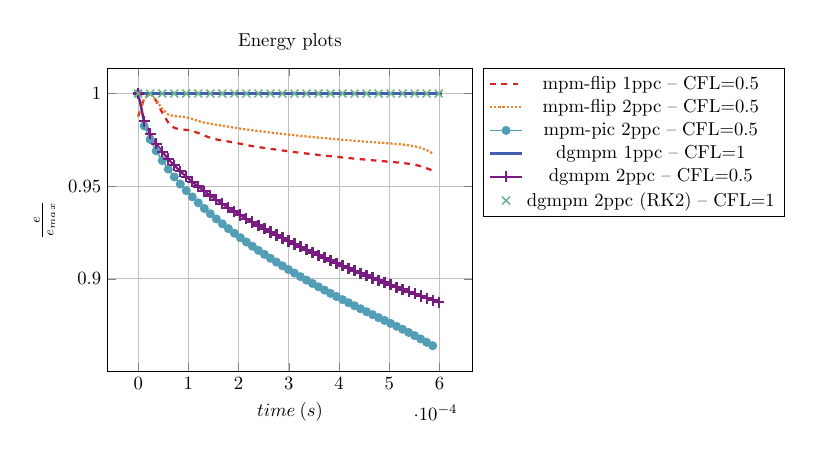
\begin{tikzpicture}[scale=.675]
\begin{axis}[xlabel=$time \: (s)$,ylabel=$\frac{e}{e_{max}}$,ymajorgrids=true,xmajorgrids=true,legend pos=outer north east,title={Energy plots}]
\addplot[Red,very thick,mark=none,dashed,mark size=2pt] coordinates {(0.0,0.987654320988) (1.2090867954e-05,0.997530864198) (2.41817359079e-05,1.0) (3.62726038619e-05,0.995910493827) (4.83634718158e-05,0.98940007716) (6.04543397698e-05,0.984093484761) (7.25452077237e-05,0.981362538279) (8.46360756777e-05,0.980572573344) (9.67269436317e-05,0.980353499636) (0.000108817811586,0.979737335844) (0.00012090867954,0.97855223305) (0.000132999547494,0.977156270039) (0.000145090415447,0.975958347691) (0.000157181283401,0.97511659562) (0.000169272151355,0.974530084065) (0.000181363019309,0.974005554053) (0.000193453887263,0.97341779498) (0.000205544755217,0.972760977912) (0.000217635623171,0.972101158286) (0.000229726491125,0.971500815494) (0.000241817359079,0.970976328432) (0.000253908227033,0.970503354023) (0.000265999094987,0.970047511625) (0.000278089962941,0.969589945626) (0.000290180830895,0.969132703566) (0.000302271698849,0.968688192138) (0.000314362566803,0.96826592316) (0.000326453434757,0.967866441189) (0.000338544302711,0.96748370195) (0.000350635170665,0.967111035083) (0.000362726038619,0.96674530374) (0.000374816906573,0.9663871534) (0.000386907774527,0.96603867283) (0.000398998642481,0.965701020803) (0.000411089510435,0.9653736209) (0.000423180378389,0.965054863002) (0.000435271246342,0.96474325827) (0.000447362114296,0.964438078134) (0.00045945298225,0.964139187671) (0.000471543850204,0.963846345834) (0.000483634718158,0.963558300848) (0.000495725586112,0.963271635613) (0.000507816454066,0.962978858237) (0.00051990732202,0.962665035247) (0.000531998189974,0.962302555824) (0.000544089057928,0.961844496637) (0.000556179925882,0.961218491107) (0.000568270793836,0.960324692645) (0.00058036166179,0.959042628999) (0.000592452529744,0.95725134199) };
\addplot[Orange,very thick,mark=none,densely dotted,mark size=3pt] coordinates {(0.0,0.987349583462) (1.19687379746e-05,0.997223079297) (2.39374759493e-05,1.0) (3.59062139239e-05,0.996543312249) (4.78749518985e-05,0.991672401699) (5.98436898731e-05,0.988645826067) (7.18124278478e-05,0.98773805255) (8.37811658224e-05,0.987631618227) (9.5749903797e-05,0.987207209533) (0.000107718641772,0.98625862112) (0.000119687379746,0.985162495947) (0.000131656117721,0.984278008796) (0.000143624855696,0.983664883566) (0.00015559359367,0.983176360212) (0.000167562331645,0.982669899583) (0.000179531069619,0.982113551237) (0.000191499807594,0.981554758898) (0.000203468545569,0.981041934115) (0.000215437283543,0.980583060318) (0.000227406021518,0.98015640132) (0.000239374759493,0.979740132791) (0.000251343497467,0.97932838866) (0.000263312235442,0.978927266369) (0.000275280973416,0.978543296202) (0.000287249711391,0.978177057907) (0.000299218449366,0.977824634311) (0.00031118718734,0.977482093196) (0.000323155925315,0.977147995987) (0.00033512466329,0.976822820567) (0.000347093401264,0.976507170495) (0.000359062139239,0.976200756538) (0.000371030877213,0.975902607469) (0.000382999615188,0.97561177268) (0.000394968353163,0.97532772239) (0.000406937091137,0.975050257459) (0.000418905829112,0.974779220922) (0.000430874567087,0.97451432881) (0.000442843305061,0.974255192075) (0.000454812043036,0.974001394871) (0.00046678078101,0.973752448152) (0.000478749518985,0.973507455428) (0.00049071825696,0.973264255861) (0.000502686994934,0.973017591891) (0.000514655732909,0.972755592972) (0.000526624470884,0.972453855054) (0.000538593208858,0.972067038786) (0.000550561946833,0.971519585751) (0.000562530684807,0.970699836135) (0.000574499422782,0.969464605892) (0.000586468160757,0.967662115176) };
\addplot[Duck,thick,mark=*,solid,mark size=2pt] coordinates {(0.0,1.0) (1.19687379746e-05,0.9825) (2.39374759493e-05,0.97517578125) (3.59062139239e-05,0.969031906128) (4.78749518985e-05,0.96380058825) (5.98436898731e-05,0.959171754479) (7.18124278478e-05,0.954982516842) (8.37811658224e-05,0.951129379832) (9.5749903797e-05,0.947543340455) (0.000107718641772,0.944175962079) (0.000119687379746,0.940991760326) (0.000131656117721,0.93796387047) (0.000143624855696,0.935071387013) (0.00015559359367,0.932297671085) (0.000167562331645,0.929629226561) (0.000179531069619,0.927054929147) (0.000191499807594,0.924565482142) (0.000203468545569,0.922153022591) (0.000215437283543,0.91981083008) (0.000227406021518,0.917533107309) (0.000239374759493,0.91531481198) (0.000251343497467,0.913151526055) (0.000263312235442,0.911039352738) (0.000275280973416,0.908974834313) (0.000287249711391,0.906954885898) (0.000299218449366,0.904976741526) (0.00031118718734,0.903037909836) (0.000323155925315,0.901136137378) (0.00033512466329,0.89926937799) (0.000347093401264,0.897435767059) (0.000359062139239,0.895633599746) (0.000371030877213,0.893861312443) (0.000382999615188,0.892117466744) (0.000394968353163,0.890400734736) (0.000406937091137,0.888709882017) (0.000418905829112,0.88704373739) (0.000430874567087,0.88540112132) (0.000442843305061,0.883780678009) (0.000454812043036,0.882180531538) (0.00046678078101,0.880597698856) (0.000478749518985,0.879027284148) (0.00049071825696,0.877461660668) (0.000502686994934,0.875890051367) (0.000514655732909,0.874299006831) (0.000526624470884,0.87267411056) (0.000538593208858,0.871002801233) (0.000550561946833,0.869277656037) (0.000562530684807,0.867499110287) (0.000574499422782,0.865676626234) (0.000586468160757,0.86382779387) };
\addplot[Blue,very thick,mark=none,solid,mark size=3pt] coordinates {(0.0,1.0) (2.41817359079e-05,1.0) (4.83634718158e-05,1.0) (7.25452077237e-05,1.0) (9.67269436317e-05,1.0) (0.00012090867954,1.0) (0.000145090415447,1.0) (0.000169272151355,1.0) (0.000193453887263,1.0) (0.000217635623171,1.0) (0.000241817359079,1.0) (0.000265999094987,1.0) (0.000290180830895,1.0) (0.000314362566803,1.0) (0.000338544302711,1.0) (0.000362726038619,1.0) (0.000386907774527,1.0) (0.000411089510435,1.0) (0.000435271246342,1.0) (0.00045945298225,1.0) (0.000483634718158,1.0) (0.000507816454066,1.0) (0.000531998189974,1.0) (0.000556179925882,1.0) (0.00058036166179,1.0) (0.000604543397698,1.0) };
\addplot[Purple,very thick,mark=+,solid,mark size=3pt] coordinates {(0.0,1.0) (1.19687379746e-05,0.985) (2.39374759493e-05,0.97828125) (3.59062139239e-05,0.972868652344) (4.78749518985e-05,0.968517532349) (5.98436898731e-05,0.964676422477) (7.18124278478e-05,0.961224535313) (8.37811658224e-05,0.95805841396) (9.5749903797e-05,0.955117021818) (0.000107718641772,0.952358340029) (0.000119687379746,0.949751847063) (0.000131656117721,0.947274776455) (0.000143624855696,0.944909512757) (0.00015559359367,0.942642119513) (0.000167562331645,0.940461338934) (0.000179531069619,0.938357922299) (0.000191499807594,0.936324160701) (0.000203468545569,0.934353548006) (0.000215437283543,0.932440533241) (0.000227406021518,0.93058033492) (0.000239374759493,0.928768799379) (0.000251343497467,0.927002291004) (0.000263312235442,0.925277605976) (0.000275280973416,0.923591903662) (0.000287249711391,0.921942651418) (0.000299218449366,0.920327579747) (0.00031118718734,0.918744645509) (0.000323155925315,0.917192001508) (0.00033512466329,0.915667971129) (0.000347093401264,0.91417102706) (0.000359062139239,0.9126997733) (0.000371030877213,0.911252929874) (0.000382999615188,0.909829319753) (0.000394968353163,0.908427857623) (0.000406937091137,0.907047540169) (0.000418905829112,0.905687437658) (0.000430874567087,0.904346686589) (0.000442843305061,0.903024483275) (0.000454812043036,0.901720078186) (0.00046678078101,0.900432770981) (0.000478749518985,0.899161906097) (0.00049071825696,0.897906868838) (0.000502686994934,0.896667081898) (0.000514655732909,0.895442002248) (0.000526624470884,0.894231118352) (0.000538593208858,0.89303394767) (0.000550561946833,0.891850034402) (0.000562530684807,0.890678947462) (0.000574499422782,0.889520278638) (0.000586468160757,0.888373640933) (0.000598436898731,0.887238667044) };
\addplot[Green,thick,mark=x,only marks,mark size=3pt] coordinates {(0.0,1.0) (2.39374759493e-05,1.0) (4.78749518985e-05,1.0) (7.18124278478e-05,1.0) (9.5749903797e-05,1.0) (0.000119687379746,1.0) (0.000143624855696,1.0) (0.000167562331645,1.0) (0.000191499807594,1.0) (0.000215437283543,1.0) (0.000239374759493,1.0) (0.000263312235442,1.0) (0.000287249711391,1.0) (0.00031118718734,1.0) (0.00033512466329,1.0) (0.000359062139239,1.0) (0.000382999615188,1.0) (0.000406937091137,1.0) (0.000430874567087,1.0) (0.000454812043036,1.0) (0.000478749518985,1.0) (0.000502686994934,1.0) (0.000526624470884,1.0) (0.000550561946833,1.0) (0.000574499422782,1.0) (0.000598436898731,1.0) };
\legend{mpm-flip 1ppc -- CFL=0.5,mpm-flip 2ppc -- CFL=0.5,mpm-pic 2ppc -- CFL=0.5,dgmpm 1ppc -- CFL=1,dgmpm 2ppc -- CFL=0.5,dgmpm 2ppc (RK2) -- CFL=1}
\end{axis}
\end{tikzpicture}
%%% Local Variables:
%%% mode: latex
%%% TeX-master: "../../presentation"
%%% End:

  \caption{Evolution of total energy $e$ for DGMPM and MPM-USL solutions on the Riemann problem in an elastic bar.}
  \label{fig:energy_elastic_RP}
\end{figure}
%%
Moreover, \textbf{the introduction of DG approximation within the USL-PIC leads to a reduction of numerical diffusion}, though less significant than that permitted by using FLIP mapping as originally proposed in the MPM.
This can be seen in figure \ref{fig:energy_elastic_RP} in which the evolution of total energies resulting from every numerical schemes is depicted.
The situations for which the CFL number is set to unity for DGMPM formulations obviously yields an exact conservation of the total energy during the computation while other results suffer from diffusion.

Since, the number of material points per cell has little influence on USL results, the MPM is from now only used with the 1ppc discretization.
Furthermore, PIC mapping has been used here within the MPM for comparison purposes and is no longer considered in the remainder simulations.
%%% Local Variables:
%%% mode: latex
%%% TeX-master: "../mainManuscript"
%%% End:


\subsection{Plane wave in a history dependent material}
\label{subsec:hpp_planewave}
We now consider a infinite medium in directions $\vect{e}_2$ and $\vect{e}_3$ and of length $l=6\:m$ in direction $\vect{e}_1$. Riemann-type initial conditions similar to those treated above are assumed to yield the following infinitesimal strain and Cauchy stress tensors:
\begin{align*}
  & \tens{\eps}= \eps \vect{e}_1 \otimes\vect{e}_1 \\
  & \tens{\sigma}=\sigma_L \vect{e}_1 \otimes \vect{e}_1 + \sigma_T \(\vect{e}_2 \otimes \vect{e}_2+\vect{e}_3 \otimes \vect{e}_3\) 
\end{align*}
which correspond to the plane wave case. In that configuration, a relation exists between longitudinal and transverse stress components $\sigma_L$ and $\sigma_T$ in such a way that a one-dimensional hyperbolic system is solved for $\sigma_L=\sigma$, and the transverse component $\sigma_T$ is computed subsequently. In this section, the behavior of the DGMPM on relaxation systems is looked at on a solid made of an elastic-viscoplastic material following Perzyna model with linear kinematic hardening \cite{Perzyna}. In the asymptotic limit $\tau = (\eta/\sigma^y)^n\rightarrow 0$, where $\tau$ is the relaxation time, the computed elastic-viscoplastic solution should tend to the elastoplastic one derived in \cite{Thomas_EP}.
The writing of the viscosity as a function of the relaxation parameter in table \ref{tab:material} enables the tuning of the stiffness of the hyperbolic system by setting different values of $\tau$.
%Table \ref{tab:material} lists the values of material parameters considered. In particular, the viscosity $\eta$ is a function of the relaxation time that is used to tune the stiffness of the problem.  

The solid is initially in a free stress state and the initial velocity is set so that plastic flow occurs:
\begin{equation*}
  v_0=2\frac{Y_H}{\rho c_L}
\end{equation*}
where $Y_H=(\lambda+2\mu)\sigma^y/2\mu$ denotes the Hugoniot elastic limit, $c_L=\sqrt{(\lambda+2\mu)/\rho}$ is the elastic pressure wave speed, and $(\lambda,\mu)$ are Lam\'e's constants. Both ends of the medium are traction free so that rightward and leftward compression elastic waves reflect as unloading waves that interact with the incident plastic ones \cite{Thomas_EVP}.

\subsubsection{Elastoviscoplasticity}
The elastic-viscoplastic problem is solved with the MPM using both USL and USF formulations, the DGMPM-Euler with Godunov splitting, and the DGMPM-RK2 coupled to Strang splitting.
The latter formulation is however not used for stiff systems since this fractional method is known to fail to assess the correct solution in those cases \cite{Thomas_EVP,Leveque_stiff}.
The ODE systems resulting from fractional approaches are discretized with an implicit backward Euler scheme for Godunov and a backward differentiation formula of order 3 for Strang splitting.
\begin{figure}[h!]
  \centering
  {\phantomsubcaption \label{subfig:evp_nonstiff1}}
  %{\phantomsubcaption \label{subfig:evp_nonstiff2}}
  {\phantomsubcaption \label{subfig:evp_nonstiff3}}
  {\begin{tikzpicture}[scale=.9]
\begin{groupplot}[group style={group size=3 by 2,
ylabels at=edge left, yticklabels at=edge left,horizontal sep=2.ex,
vertical sep=4ex,xticklabels at=edge bottom,xlabels at=edge bottom},
ymajorgrids=true,xmajorgrids=true,enlargelimits=0,xmin=0.,xmax=6.,xlabel=$x (m)$,
axis on top,scale only axis,width=0.32\linewidth
]
\nextgroupplot[ylabel=$\sigma (Pa)$,title={(a) $t = 4.17\times 10^{-4} $ s.},ymin=-1545202237.9160104,ymax=42415827.93308663,]
\addplot[Red,dashed,mark=none,very thick,mark size=3pt,mark repeat=2] coordinates{(0.0,-9466083.71137175) (0.12244897959183673,-35514206.734367736) (0.24489795918367346,-84113776.24908806) (0.36734693877551017,-172446629.58542818) (0.4897959183673469,-314805947.20807856) (0.6122448979591837,-511629446.98755276) (0.7346938775510203,-736313113.7069598) (0.8571428571428571,-931144828.2647986) (0.9795918367346939,-1068053644.3292406) (1.1020408163265305,-1170764300.0847378) (1.2244897959183674,-1252110103.6024575) (1.346938775510204,-1302676056.5462253) (1.4693877551020407,-1310165737.6186237) (1.5918367346938775,-1279757193.7171304) (1.7142857142857142,-1256553263.265204) (1.836734693877551,-1258006223.1072822) (1.9591836734693877,-1294050482.3234062) (2.0816326530612246,-1300642620.5987113) (2.204081632653061,-1307227334.5769467) (2.326530612244898,-1275303748.496001) (2.4489795918367347,-1289208797.7645764) (2.571428571428571,-1280826893.2226717) (2.693877551020408,-1303157436.709725) (2.816326530612245,-1289006021.9435475) (2.9387755102040813,-1289002398.658552) (3.061224489795918,-1289002460.452313) (3.183673469387755,-1289006071.890395) (3.306122448979592,-1303157225.279095) (3.4285714285714284,-1280827082.3206232) (3.5510204081632653,-1289208893.7221813) (3.673469387755102,-1275303766.5179212) (3.7959183673469385,-1307227387.3540978) (3.9183673469387754,-1300642664.183363) (4.040816326530612,-1294050357.0073159) (4.163265306122449,-1258006259.974342) (4.285714285714286,-1256553191.759347) (4.408163265306122,-1279757267.3487592) (4.530612244897959,-1310165771.052653) (4.653061224489796,-1302676007.627941) (4.775510204081632,-1252110079.6983936) (4.8979591836734695,-1170764547.776224) (5.020408163265306,-1068053501.3343573) (5.142857142857142,-931144730.4547592) (5.26530612244898,-736313057.6797745) (5.387755102040816,-511629430.76423925) (5.5102040816326525,-314805938.17461526) (5.63265306122449,-172446625.3783345) (5.755102040816326,-84113774.55431706) (5.877551020408163,-35514206.14830053) (6.0,-9466083.577332078) };
\addplot[Orange,dotted,mark=none,very thick,mark size=3pt,mark repeat=2] coordinates{(0.0,-21775616.685123403) (0.12244897959183673,-21775616.72164698) (0.24489795918367346,-112154769.91343763) (0.36734693877551017,-112154770.19419384) (0.4897959183673469,-357061973.86971843) (0.6122448979591837,-357061975.87384665) (0.7346938775510203,-790799603.3382715) (0.8571428571428571,-790799622.7090364) (0.9795918367346939,-1127863861.8971207) (1.1020408163265305,-1127863910.7156112) (1.2244897959183674,-1294097542.9943345) (1.346938775510204,-1294097833.9624486) (1.4693877551020407,-1264908473.5999227) (1.5918367346938775,-1264908907.9452155) (1.7142857142857142,-1170899419.842339) (1.836734693877551,-1170898869.1188018) (1.9591836734693877,-1404729307.196373) (2.0816326530612246,-1404729023.510617) (2.204081632653061,-1178030994.2246718) (2.326530612244898,-1178032103.900689) (2.4489795918367347,-1325532527.4682536) (2.571428571428571,-1325532662.4079945) (2.693877551020408,-1286992617.5223172) (2.816326530612245,-1286992228.933896) (2.9387755102040813,-1254505712.3434386) (3.061224489795918,-1254505904.1655023) (3.183673469387755,-1286992713.028294) (3.306122448979592,-1286993281.7005486) (3.4285714285714284,-1325532286.4512568) (3.5510204081632653,-1325532447.008532) (3.673469387755102,-1178031216.3396027) (3.7959183673469385,-1178031165.6288564) (3.9183673469387754,-1404729070.936975) (4.040816326530612,-1404729206.2986672) (4.163265306122449,-1170899488.2777543) (4.285714285714286,-1170899253.556783) (4.408163265306122,-1264908724.8211215) (4.530612244897959,-1264908806.5057957) (4.653061224489796,-1294097602.037558) (4.775510204081632,-1294097585.2606838) (4.8979591836734695,-1127863890.5307767) (5.020408163265306,-1127863857.5211554) (5.142857142857142,-790799615.9051313) (5.26530612244898,-790799601.5180427) (5.387755102040816,-357061976.4955751) (5.5102040816326525,-357061973.8588882) (5.63265306122449,-112154770.18131427) (5.755102040816326,-112154769.96143283) (5.877551020408163,-21775616.70163) (6.0,-21775616.698375184) };
\addplot[Blue,solid,mark=none,very thick,mark size=3pt,mark repeat=2] coordinates{(0.0,-6.648826343127885e-07) (0.12244897959183673,4.986619757345916e-07) (0.24489795918367346,-6.648826343127894e-07) (0.36734693877551017,6.648826343127889e-07) (0.4897959183673469,-3.324413171563951e-07) (0.6122448979591837,-874162257.8546059) (0.7346938775510203,-913424760.9782704) (0.8571428571428571,-969365384.6175718) (0.9795918367346939,-1042970790.4967976) (1.1020408163265305,-1132583339.8680727) (1.2244897959183674,-1201739241.5745146) (1.346938775510204,-1248614593.9146428) (1.4693877551020407,-1253812053.171889) (1.5918367346938775,-1277494278.936118) (1.7142857142857142,-1268975112.888906) (1.836734693877551,-1285312313.5954506) (1.9591836734693877,-1275249588.3375967) (2.0816326530612246,-1288549436.3162062) (2.204081632653061,-1278115488.7494104) (2.326530612244898,-1289609709.5365772) (2.4489795918367347,-1280020503.890194) (2.571428571428571,-1288883802.6033092) (2.693877551020408,-1282041862.894144) (2.816326530612245,-1286896451.527247) (2.9387755102040813,-1284697650.7072186) (3.061224489795918,-1284697650.7072196) (3.183673469387755,-1286896451.5272474) (3.306122448979592,-1282041862.8941436) (3.4285714285714284,-1288883802.6033094) (3.5510204081632653,-1280020503.890194) (3.673469387755102,-1289609709.5365787) (3.7959183673469385,-1278115488.74941) (3.9183673469387754,-1288549436.3162065) (4.040816326530612,-1275249588.337598) (4.163265306122449,-1285312313.5954502) (4.285714285714286,-1268975112.8889062) (4.408163265306122,-1277494278.9361184) (4.530612244897959,-1253812053.1718888) (4.653061224489796,-1248614593.914643) (4.775510204081632,-1201739241.5745142) (4.8979591836734695,-1132583339.8680727) (5.020408163265306,-1042970790.496798) (5.142857142857142,-969365384.6175721) (5.26530612244898,-913424760.9782704) (5.387755102040816,-874162257.8546067) (5.5102040816326525,6.648826343127891e-07) (5.63265306122449,-8.311032928909869e-07) (5.755102040816326,6.64882634312789e-07) (5.877551020408163,-4.986619757345927e-07) (6.0,6.648826343127891e-07) };
\addplot[Purple,solid,mark=+,very thick,mark size=3pt,mark repeat=2] coordinates{(0.0,-11522502.92600226) (0.06060606060606061,-31725620.091397233) (0.12121212121212122,-61304874.4765079) (0.18181818181818182,-93259931.32451278) (0.24242424242424243,-140838495.245558) (0.30303030303030304,-193913468.55103528) (0.36363636363636365,-265213878.38892987) (0.42424242424242425,-342130694.52595234) (0.48484848484848486,-432453677.3208593) (0.5454545454545454,-525041147.1169883) (0.6060606060606061,-618338331.152021) (0.6666666666666667,-708388503.4017504) (0.7272727272727273,-784021969.6614887) (0.7878787878787878,-850474949.5391626) (0.8484848484848485,-896076004.6724114) (0.9090909090909092,-935262643.3934776) (0.9696969696969697,-969337341.7916008) (1.0303030303030303,-1004304635.4591644) (1.0909090909090908,-1040567603.2284905) (1.1515151515151516,-1077307888.8979723) (1.2121212121212122,-1112635201.8637893) (1.2727272727272727,-1146677662.6062891) (1.3333333333333335,-1175184951.6380641) (1.393939393939394,-1201590500.124662) (1.4545454545454546,-1220740340.2067573) (1.5151515151515151,-1238089436.820448) (1.5757575757575757,-1249284876.1027403) (1.6363636363636365,-1259440830.6822593) (1.696969696969697,-1265589775.602502) (1.7575757575757576,-1271283785.6788774) (1.8181818181818183,-1274687789.8815384) (1.878787878787879,-1277922433.571672) (1.9393939393939394,-1279879339.775472) (2.0,-1281783669.6916373) (2.0606060606060606,-1282949267.7273479) (2.121212121212121,-1284109224.9776726) (2.1818181818181817,-1284819623.1742642) (2.2424242424242427,-1285544784.5476487) (2.303030303030303,-1285981972.386752) (2.3636363636363638,-1286442996.2191055) (2.4242424242424243,-1286710383.2766345) (2.484848484848485,-1287006241.599304) (2.5454545454545454,-1287165476.0382879) (2.606060606060606,-1287356422.5321994) (2.666666666666667,-1287445575.37196) (2.7272727272727275,-1287570603.4105794) (2.787878787878788,-1287613773.5740457) (2.8484848484848486,-1287701397.1398175) (2.909090909090909,-1287711163.0639696) (2.9696969696969697,-1287803837.1394258) (3.0303030303030303,-1287803837.1394258) (3.090909090909091,-1287711163.0639691) (3.1515151515151514,-1287701397.1398172) (3.2121212121212124,-1287613773.5740457) (3.272727272727273,-1287570603.4105797) (3.3333333333333335,-1287445575.37196) (3.393939393939394,-1287356422.5321996) (3.4545454545454546,-1287165476.038288) (3.515151515151515,-1287006241.5993047) (3.5757575757575757,-1286710383.276635) (3.6363636363636367,-1286442996.2191057) (3.6969696969696972,-1285981972.386752) (3.757575757575758,-1285544784.547649) (3.8181818181818183,-1284819623.1742642) (3.878787878787879,-1284109224.977673) (3.9393939393939394,-1282949267.7273483) (4.0,-1281783669.6916378) (4.0606060606060606,-1279879339.7754729) (4.121212121212121,-1277922433.571673) (4.181818181818182,-1274687789.881539) (4.242424242424242,-1271283785.678878) (4.303030303030303,-1265589775.602503) (4.363636363636363,-1259440830.6822598) (4.424242424242425,-1249284876.1027408) (4.484848484848485,-1238089436.8204484) (4.545454545454546,-1220740340.206758) (4.606060606060606,-1201590500.124663) (4.666666666666667,-1175184951.6380656) (4.7272727272727275,-1146677662.60629) (4.787878787878788,-1112635201.8637903) (4.848484848484849,-1077307888.8979728) (4.909090909090909,-1040567603.2284908) (4.96969696969697,-1004304635.459165) (5.03030303030303,-969337341.7916014) (5.090909090909091,-935262643.3934779) (5.151515151515151,-896076004.6724123) (5.212121212121212,-850474949.5391635) (5.2727272727272725,-784021969.6614897) (5.333333333333334,-708388503.401751) (5.3939393939393945,-618338331.1520219) (5.454545454545455,-525041147.11698914) (5.515151515151516,-432453677.3208602) (5.575757575757576,-342130694.5259528) (5.636363636363637,-265213878.3889301) (5.696969696969697,-193913468.55103546) (5.757575757575758,-140838495.24555832) (5.818181818181818,-93259931.3245125) (5.878787878787879,-61304874.4765082) (5.9393939393939394,-31725620.091397557) (6.0,-11522502.926002609) };
\addplot[Green,only marks,mark=x,thick,mark size=3pt,mark repeat=2] coordinates{(0.0,-2.0877147917780336e-07) (0.06060606060606061,-1.23669837978591e-07) (0.12121212121212122,1.0131895444177197e-06) (0.18181818181818182,9.814583585206487e-07) (0.24242424242424243,-5.619879278457838e-07) (0.30303030303030304,-7.677773407797948e-07) (0.36363636363636365,4.815476698956227e-07) (0.42424242424242425,1.8333496441716677e-07) (0.48484848484848486,1.0440135561077701e-07) (0.5454545454545454,2.2803996154561766e-07) (0.6060606060606061,-884550714.70502) (0.6666666666666667,-884550714.7050202) (0.7272727272727273,-936122014.0999393) (0.7878787878787878,-936122014.0999395) (0.8484848484848485,-1010904183.587626) (0.9090909090909092,-1010904183.5876261) (0.9696969696969697,-1105134845.294078) (1.0303030303030303,-1105134845.294077) (1.0909090909090908,-1200693543.9954407) (1.1515151515151516,-1200693543.9954407) (1.2121212121212122,-1242600895.2828481) (1.2727272727272727,-1242600895.2828481) (1.3333333333333335,-1280378553.9593801) (1.393939393939394,-1280378553.9593809) (1.4545454545454546,-1275721452.5659273) (1.5151515151515151,-1275721452.5659602) (1.5757575757575757,-1300299286.3908393) (1.6363636363636365,-1300299286.3908374) (1.696969696969697,-1289272425.5395763) (1.7575757575757576,-1289272425.5395694) (1.8181818181818183,-1306127301.5683103) (1.878787878787879,-1306127301.5683022) (1.9393939393939394,-1296028797.1903882) (2.0,-1296028797.1903853) (2.0606060606060606,-1308123608.354041) (2.121212121212121,-1308123608.3541112) (2.1818181818181817,-1299597735.2461388) (2.2424242424242427,-1299597735.246238) (2.303030303030303,-1308620980.1784377) (2.3636363636363638,-1308620980.1784313) (2.4242424242424243,-1301801281.3713925) (2.484848484848485,-1301801281.3713658) (2.5454545454545454,-1308121765.4283872) (2.606060606060606,-1308121765.4283755) (2.666666666666667,-1303587683.0677166) (2.7272727272727275,-1303587683.0677037) (2.787878787878788,-1306911469.4399674) (2.8484848484848486,-1306911469.4400563) (2.909090909090909,-1305310135.1663263) (2.9696969696969697,-1305310135.1662202) (3.0303030303030303,-1305310135.1663122) (3.090909090909091,-1305310135.1663315) (3.1515151515151514,-1306911469.4400697) (3.2121212121212124,-1306911469.4400973) (3.272727272727273,-1303587683.067521) (3.3333333333333335,-1303587683.0675333) (3.393939393939394,-1308121765.428341) (3.4545454545454546,-1308121765.4283326) (3.515151515151515,-1301801281.3712707) (3.5757575757575757,-1301801281.3712776) (3.6363636363636367,-1308620980.1785724) (3.6969696969696972,-1308620980.1785636) (3.757575757575758,-1299597735.2460728) (3.8181818181818183,-1299597735.2461448) (3.878787878787879,-1308123608.3541088) (3.9393939393939394,-1308123608.3540418) (4.0,-1296028797.1904147) (4.0606060606060606,-1296028797.190405) (4.121212121212121,-1306127301.5683162) (4.181818181818182,-1306127301.5683157) (4.242424242424242,-1289272425.5394864) (4.303030303030303,-1289272425.5394852) (4.363636363636363,-1300299286.390773) (4.424242424242425,-1300299286.3907716) (4.484848484848485,-1275721452.565949) (4.545454545454546,-1275721452.565983) (4.606060606060606,-1280378553.9593606) (4.666666666666667,-1280378553.9593616) (4.7272727272727275,-1242600895.2828217) (4.787878787878788,-1242600895.2828217) (4.848484848484849,-1200693543.9954677) (4.909090909090909,-1200693543.9954684) (4.96969696969697,-1105134845.294094) (5.03030303030303,-1105134845.2940938) (5.090909090909091,-1010904183.5876323) (5.151515151515151,-1010904183.5876321) (5.212121212121212,-936122014.0999426) (5.2727272727272725,-936122014.0999423) (5.333333333333334,-884550714.7050228) (5.3939393939393945,-884550714.7050234) (5.454545454545455,6.698192810303248e-07) (5.515151515151516,6.599459875952535e-07) (5.575757575757576,-9.369788715662316e-07) (5.636363636363637,-1.0576690313721361e-06) (5.696969696969697,1.675441116120912e-06) (5.757575757575758,1.6489720554430353e-06) (5.818181818181818,-1.0608989471845062e-06) (5.878787878787879,-9.337489557538617e-07) (5.9393939393939394,1.4751713795395358e-06) (6.0,1.5168004748680168e-06) };
\addplot[black,solid,mark=none,thin,mark size=3pt,mark repeat=2] coordinates{(0.0,-0.0) (0.12244897959183673,-0.0) (0.24489795918367346,-0.0) (0.36734693877551017,-0.0) (0.4897959183673469,-0.0) (0.6122448979591837,-700000000.0) (0.7346938775510203,-700000000.0) (0.8571428571428571,-700000000.0) (0.9795918367346939,-700000000.0) (1.1020408163265305,-1261004576.260559) (1.2244897959183674,-1261004576.260559) (1.346938775510204,-1261004576.260559) (1.4693877551020407,-1261004576.260559) (1.5918367346938775,-1261004576.260559) (1.7142857142857142,-1261004576.260559) (1.836734693877551,-1261004576.260559) (1.9591836734693877,-1261004576.260559) (2.0816326530612246,-1261004576.260559) (2.204081632653061,-1261004576.260559) (2.326530612244898,-1261004576.260559) (2.4489795918367347,-1261004576.260559) (2.571428571428571,-1261004576.260559) (2.693877551020408,-1261004576.260559) (2.816326530612245,-1261004576.260559) (2.9387755102040813,-1261004576.260559) (3.061224489795918,-1261004576.260559) (3.183673469387755,-1261004576.260559) (3.306122448979592,-1261004576.260559) (3.4285714285714284,-1261004576.260559) (3.5510204081632653,-1261004576.260559) (3.673469387755102,-1261004576.260559) (3.7959183673469385,-1261004576.260559) (3.9183673469387754,-1261004576.260559) (4.040816326530612,-1261004576.260559) (4.163265306122449,-1261004576.260559) (4.285714285714286,-1261004576.260559) (4.408163265306122,-1261004576.260559) (4.530612244897959,-1261004576.260559) (4.653061224489796,-1261004576.260559) (4.775510204081632,-1261004576.260559) (4.8979591836734695,-1261004576.260559) (5.020408163265306,-700000000.0) (5.142857142857142,-700000000.0) (5.26530612244898,-700000000.0) (5.387755102040816,-700000000.0) (5.5102040816326525,-0.0) (5.63265306122449,-0.0) (5.755102040816326,-0.0) (5.877551020408163,-0.0) (6.0,-0.0) };
\nextgroupplot[title={(b) $t = 6.25\times 10^{-4} $ s.},ymin=-1545202237.9160104,ymax=42415827.93308663,]
\addplot[Red,dashed,mark=none,very thick,mark size=3pt,mark repeat=2] coordinates{(0.0,-68320403.62221353) (0.12244897959183673,-225789676.02918974) (0.24489795918367346,-424791619.04833) (0.36734693877551017,-646380796.7713014) (0.4897959183673469,-849944016.2028724) (0.6122448979591837,-1006146061.0400205) (0.7346938775510203,-1114292580.0561018) (0.8571428571428571,-1188728982.2247245) (0.9795918367346939,-1241700251.4602263) (1.1020408163265305,-1273020972.5655205) (1.2244897959183674,-1284949093.1656094) (1.346938775510204,-1280762376.3082383) (1.4693877551020407,-1280131918.3035223) (1.5918367346938775,-1279490959.2062156) (1.7142857142857142,-1290763235.7380192) (1.836734693877551,-1286886471.7575386) (1.9591836734693877,-1293425757.5226574) (2.0816326530612246,-1281287553.8251324) (2.204081632653061,-1292409766.4422443) (2.326530612244898,-1282629752.438702) (2.4489795918367347,-1294945401.113779) (2.571428571428571,-1283794612.9732673) (2.693877551020408,-1291887694.9803798) (2.816326530612245,-1285785861.1559482) (2.9387755102040813,-1289860908.4664276) (3.061224489795918,-1289860960.9809775) (3.183673469387755,-1285785837.4934893) (3.306122448979592,-1291887487.9744287) (3.4285714285714284,-1283794664.8462174) (3.5510204081632653,-1294945447.7560375) (3.673469387755102,-1282629760.5221589) (3.7959183673469385,-1292409767.8294322) (3.9183673469387754,-1281287565.3495717) (4.040816326530612,-1293425764.3679597) (4.163265306122449,-1286886489.0287468) (4.285714285714286,-1290763226.34359) (4.408163265306122,-1279490965.7329388) (4.530612244897959,-1280131956.1996849) (4.653061224489796,-1280762451.4159694) (4.775510204081632,-1284949184.1714568) (4.8979591836734695,-1273020948.2916741) (5.020408163265306,-1241700137.1761186) (5.142857142857142,-1188728796.523432) (5.26530612244898,-1114292407.0488575) (5.387755102040816,-1006146274.5465661) (5.5102040816326525,-849944214.1880462) (5.63265306122449,-646381051.5707061) (5.755102040816326,-424791730.9041514) (5.877551020408163,-225789800.60525674) (6.0,-68320454.65089296) };
\addplot[Orange,dotted,mark=none,very thick,mark size=3pt,mark repeat=2] coordinates{(0.0,-156995048.72300234) (0.12244897959183673,-156995364.03184575) (0.24489795918367346,-578361553.8773596) (0.36734693877551017,-578361776.9652294) (0.4897959183673469,-947878572.789029) (0.6122448979591837,-947878629.0454134) (0.7346938775510203,-1122155365.9445817) (0.8571428571428571,-1122155222.890123) (0.9795918367346939,-1291825792.2012048) (1.1020408163265305,-1291825773.3810687) (1.2244897959183674,-1251635171.0476031) (1.346938775510204,-1251635100.0260744) (1.4693877551020407,-1232474111.1713145) (1.5918367346938775,-1232473886.0470812) (1.7142857142857142,-1376816804.9626572) (1.836734693877551,-1376817081.1171806) (1.9591836734693877,-1157922444.4640186) (2.0816326530612246,-1157922510.7665095) (2.204081632653061,-1403184236.5989518) (2.326530612244898,-1403184536.0603929) (2.4489795918367347,-1180859401.2507882) (2.571428571428571,-1180859508.133819) (2.693877551020408,-1368793239.5548983) (2.816326530612245,-1368793451.4344292) (2.9387755102040813,-1203835945.0107105) (3.061224489795918,-1203835622.7844667) (3.183673469387755,-1368793306.427742) (3.306122448979592,-1368793478.6580884) (3.4285714285714284,-1180859183.8880649) (3.5510204081632653,-1180859290.5038683) (3.673469387755102,-1403184136.6867287) (3.7959183673469385,-1403183761.77251) (3.9183673469387754,-1157922482.3658946) (4.040816326530612,-1157922352.2307622) (4.163265306122449,-1376817001.1907525) (4.285714285714286,-1376817315.2298005) (4.408163265306122,-1232474572.3256762) (4.530612244897959,-1232474451.4669452) (4.653061224489796,-1251634884.2142015) (4.775510204081632,-1251635269.3170545) (4.8979591836734695,-1291825665.5679488) (5.020408163265306,-1291825906.6643884) (5.142857142857142,-1122155225.5621386) (5.26530612244898,-1122155914.2048798) (5.387755102040816,-947878625.770502) (5.5102040816326525,-947877795.5933025) (5.63265306122449,-578361684.1093763) (5.755102040816326,-578362214.7513508) (5.877551020408163,-156995223.63768175) (6.0,-156995328.8817121) };
\addplot[Blue,solid,mark=none,very thick,mark size=3pt,mark repeat=2] coordinates{(0.0,-78094246.59211227) (0.12244897959183673,-202047177.96964124) (0.24489795918367346,-306454110.06972677) (0.36734693877551017,-380145390.26078814) (0.4897959183673469,-423404735.09272164) (0.6122448979591837,-1257853636.3109157) (0.7346938775510203,-1257085473.8466249) (0.8571428571428571,-1273738336.1650534) (0.9795918367346939,-1266172602.6079874) (1.1020408163265305,-1281249763.7189615) (1.2244897959183674,-1270901976.3756995) (1.346938775510204,-1284583664.611882) (1.4693877551020407,-1273997234.574172) (1.5918367346938775,-1285577300.0190902) (1.7142857142857142,-1276400493.5524273) (1.836734693877551,-1285417293.975184) (1.9591836734693877,-1278339664.6925926) (2.0816326530612246,-1284852686.1476386) (2.204081632653061,-1279850028.976812) (2.326530612244898,-1284238970.623943) (2.4489795918367347,-1280987011.9763784) (2.571428571428571,-1283670980.1448214) (2.693877551020408,-1281846768.3113825) (2.816326530612245,-1283114948.4817128) (2.9387755102040813,-1282695202.1981924) (3.061224489795918,-1282695202.1981914) (3.183673469387755,-1283114948.4817138) (3.306122448979592,-1281846768.3113823) (3.4285714285714284,-1283670980.1448233) (3.5510204081632653,-1280987011.9763772) (3.673469387755102,-1284238970.6239436) (3.7959183673469385,-1279850028.9768124) (3.9183673469387754,-1284852686.147639) (4.040816326530612,-1278339664.6925926) (4.163265306122449,-1285417293.9751842) (4.285714285714286,-1276400493.5524268) (4.408163265306122,-1285577300.0190902) (4.530612244897959,-1273997234.5741723) (4.653061224489796,-1284583664.6118824) (4.775510204081632,-1270901976.3757002) (4.8979591836734695,-1281249763.718962) (5.020408163265306,-1266172602.6079872) (5.142857142857142,-1273738336.1650534) (5.26530612244898,-1257085473.8466249) (5.387755102040816,-1257853636.3109152) (5.5102040816326525,-423404735.092723) (5.63265306122449,-380145390.2607865) (5.755102040816326,-306454110.0697275) (5.877551020408163,-202047177.96964) (6.0,-78094246.59211358) };
\addplot[Purple,solid,mark=+,very thick,mark size=3pt,mark repeat=2] coordinates{(0.0,-29927303.866736423) (0.06060606060606061,-91056397.63368599) (0.12121212121212122,-151613704.523153) (0.18181818181818182,-216112605.28132087) (0.24242424242424243,-280335641.2622369) (0.30303030303030304,-352344393.75337386) (0.36363636363636365,-424489613.7233627) (0.42424242424242425,-505847292.410384) (0.48484848484848486,-586999789.9597377) (0.5454545454545454,-673998041.6926832) (0.6060606060606061,-759351839.9800754) (0.6666666666666667,-843513643.4035325) (0.7272727272727273,-923946644.5385387) (0.7878787878787878,-995414783.6619084) (0.8484848484848485,-1061232446.5295665) (0.9090909090909092,-1113218962.1696506) (0.9696969696969697,-1159051731.4367843) (1.0303030303030303,-1191404581.2317898) (1.0909090909090908,-1218844186.0222213) (1.1515151515151516,-1236684855.8963497) (1.2121212121212122,-1251383919.797765) (1.2727272727272727,-1260493728.1975224) (1.3333333333333335,-1267812955.7854612) (1.393939393939394,-1272272932.5908973) (1.4545454545454546,-1275765921.540089) (1.5151515151515151,-1277936320.3680944) (1.5757575757575757,-1279592582.5775201) (1.6363636363636365,-1280693510.9832897) (1.696969696969697,-1281513981.0637147) (1.7575757575757576,-1282125151.9012914) (1.8181818181818183,-1282572071.178818) (1.878787878787879,-1282950867.4850798) (1.9393939393939394,-1283223494.4286144) (2.0,-1283480133.76503) (2.0606060606060606,-1283661506.7126255) (2.121212121212121,-1283844490.520339) (2.1818181818181817,-1283970476.588324) (2.2424242424242427,-1284103730.0809987) (2.303030303030303,-1284191946.2274148) (2.3636363636363638,-1284289437.5825508) (2.4242424242424243,-1284350224.7858446) (2.484848484848485,-1284421413.7540164) (2.5454545454545454,-1284461770.7762535) (2.606060606060606,-1284513746.332839) (2.666666666666667,-1284538764.3494127) (2.7272727272727275,-1284577367.2906) (2.787878787878788,-1284590745.1308227) (2.8484848484848486,-1284621851.9102542) (2.909090909090909,-1284624878.9151099) (2.9696969696969697,-1284663796.6518083) (3.0303030303030303,-1284663796.6518083) (3.090909090909091,-1284624878.9151099) (3.1515151515151514,-1284621851.9102545) (3.2121212121212124,-1284590745.1308224) (3.272727272727273,-1284577367.2906) (3.3333333333333335,-1284538764.3494127) (3.393939393939394,-1284513746.332839) (3.4545454545454546,-1284461770.7762532) (3.515151515151515,-1284421413.7540162) (3.5757575757575757,-1284350224.7858446) (3.6363636363636367,-1284289437.582551) (3.6969696969696972,-1284191946.227415) (3.757575757575758,-1284103730.0809991) (3.8181818181818183,-1283970476.5883245) (3.878787878787879,-1283844490.5203397) (3.9393939393939394,-1283661506.712626) (4.0,-1283480133.7650306) (4.0606060606060606,-1283223494.4286153) (4.121212121212121,-1282950867.4850807) (4.181818181818182,-1282572071.1788187) (4.242424242424242,-1282125151.901292) (4.303030303030303,-1281513981.0637155) (4.363636363636363,-1280693510.9832904) (4.424242424242425,-1279592582.577521) (4.484848484848485,-1277936320.3680952) (4.545454545454546,-1275765921.5400894) (4.606060606060606,-1272272932.5908978) (4.666666666666667,-1267812955.785462) (4.7272727272727275,-1260493728.1975229) (4.787878787878788,-1251383919.797766) (4.848484848484849,-1236684855.8963506) (4.909090909090909,-1218844186.0222228) (4.96969696969697,-1191404581.231791) (5.03030303030303,-1159051731.4367847) (5.090909090909091,-1113218962.169651) (5.151515151515151,-1061232446.529567) (5.212121212121212,-995414783.6619091) (5.2727272727272725,-923946644.5385387) (5.333333333333334,-843513643.4035326) (5.3939393939393945,-759351839.9800754) (5.454545454545455,-673998041.6926835) (5.515151515151516,-586999789.9597379) (5.575757575757576,-505847292.4103844) (5.636363636363637,-424489613.7233631) (5.696969696969697,-352344393.7533744) (5.757575757575758,-280335641.2622374) (5.818181818181818,-216112605.28132126) (5.878787878787879,-151613704.5231535) (5.9393939393939394,-91056397.63368621) (6.0,-29927303.86673645) };
\addplot[Green,only marks,mark=x,thick,mark size=3pt,mark repeat=2] coordinates{(0.0,-79916002.67055239) (0.06060606060606061,-79916002.67055224) (0.12121212121212122,-212751355.9722632) (0.18181818181818182,-212751355.97226292) (0.24242424242424243,-312518540.6021343) (0.30303030303030304,-312518540.60213417) (0.36363636363636365,-394252960.7380532) (0.42424242424242425,-394252960.73804915) (0.48484848484848486,-435228881.2798793) (0.5454545454545454,-435228881.27987766) (0.6060606060606061,-1285411981.4217432) (0.6666666666666667,-1285411981.4217405) (0.7272727272727273,-1280711603.3230183) (0.7878787878787878,-1280711603.3230135) (0.8484848484848485,-1295937493.3862524) (0.9090909090909092,-1295937493.3862624) (0.9696969696969697,-1287988489.6130652) (1.0303030303030303,-1287988489.6129992) (1.0909090909090908,-1301349142.6084783) (1.1515151515151516,-1301349142.6085305) (1.2121212121212122,-1292031977.182477) (1.2727272727272727,-1292031977.1824605) (1.3333333333333335,-1304158962.6097703) (1.393939393939394,-1304158962.609774) (1.4545454545454546,-1294615911.7133598) (1.5151515151515151,-1294615911.713364) (1.5757575757575757,-1305409469.234389) (1.6363636363636365,-1305409469.2343793) (1.696969696969697,-1296575097.169732) (1.7575757575757576,-1296575097.1696386) (1.8181818181818183,-1305694934.8057256) (1.878787878787879,-1305694934.8056414) (1.9393939393939394,-1298237888.1883545) (2.0,-1298237888.1883388) (2.0606060606060606,-1305422829.3343308) (2.121212121212121,-1305422829.3343291) (2.1818181818181817,-1299681183.8928425) (2.2424242424242427,-1299681183.8927386) (2.303030303030303,-1304867646.3713446) (2.3636363636363638,-1304867646.3713348) (2.4242424242424243,-1300902385.280055) (2.484848484848485,-1300902385.280057) (2.5454545454545454,-1304201666.8734922) (2.606060606060606,-1304201666.8733885) (2.666666666666667,-1301910986.9763758) (2.7272727272727275,-1301910986.9763756) (2.787878787878788,-1303498906.5357742) (2.8484848484848486,-1303498906.535786) (2.909090909090909,-1302755121.5435212) (2.9696969696969697,-1302755121.5435221) (3.0303030303030303,-1302755121.543637) (3.090909090909091,-1302755121.543634) (3.1515151515151514,-1303498906.5355883) (3.2121212121212124,-1303498906.5355833) (3.272727272727273,-1301910986.97636) (3.3333333333333335,-1301910986.9762814) (3.393939393939394,-1304201666.8734074) (3.4545454545454546,-1304201666.8733807) (3.515151515151515,-1300902385.280354) (3.5757575757575757,-1300902385.2803435) (3.6363636363636367,-1304867646.3712885) (3.6969696969696972,-1304867646.3712816) (3.757575757575758,-1299681183.8926687) (3.8181818181818183,-1299681183.8927484) (3.878787878787879,-1305422829.3345184) (3.9393939393939394,-1305422829.3345306) (4.0,-1298237888.1883025) (4.0606060606060606,-1298237888.1882656) (4.121212121212121,-1305694934.8057399) (4.181818181818182,-1305694934.8057516) (4.242424242424242,-1296575097.1697433) (4.303030303030303,-1296575097.1697195) (4.363636363636363,-1305409469.2346466) (4.424242424242425,-1305409469.2346435) (4.484848484848485,-1294615911.7133439) (4.545454545454546,-1294615911.713418) (4.606060606060606,-1304158962.609734) (4.666666666666667,-1304158962.6097326) (4.7272727272727275,-1292031977.1825411) (4.787878787878788,-1292031977.1825192) (4.848484848484849,-1301349142.6085944) (4.909090909090909,-1301349142.6086338) (4.96969696969697,-1287988489.6129642) (5.03030303030303,-1287988489.6129599) (5.090909090909091,-1295937493.3861973) (5.151515151515151,-1295937493.38624) (5.212121212121212,-1280711603.3229506) (5.2727272727272725,-1280711603.3229578) (5.333333333333334,-1285411981.4217515) (5.3939393939393945,-1285411981.4217482) (5.454545454545455,-435228881.27979714) (5.515151515151516,-435228881.2797981) (5.575757575757576,-394252960.7380172) (5.636363636363637,-394252960.7380113) (5.696969696969697,-312518540.6021377) (5.757575757575758,-312518540.6021374) (5.818181818181818,-212751355.9722441) (5.878787878787879,-212751355.97224396) (5.9393939393939394,-79916002.67054233) (6.0,-79916002.67054217) };
\addplot[black,solid,mark=none,thin,mark size=3pt,mark repeat=2] coordinates{(0.0,-0.0) (0.12244897959183673,-630502288.1302795) (0.24489795918367346,-630502288.1302795) (0.36734693877551017,-630502288.1302795) (0.4897959183673469,-630502288.1302795) (0.6122448979591837,-1261004576.260559) (0.7346938775510203,-1261004576.260559) (0.8571428571428571,-1261004576.260559) (0.9795918367346939,-1261004576.260559) (1.1020408163265305,-1261004576.260559) (1.2244897959183674,-1261004576.260559) (1.346938775510204,-1261004576.260559) (1.4693877551020407,-1261004576.260559) (1.5918367346938775,-1261004576.260559) (1.7142857142857142,-1261004576.260559) (1.836734693877551,-1261004576.260559) (1.9591836734693877,-1261004576.260559) (2.0816326530612246,-1261004576.260559) (2.204081632653061,-1261004576.260559) (2.326530612244898,-1261004576.260559) (2.4489795918367347,-1261004576.260559) (2.571428571428571,-1261004576.260559) (2.693877551020408,-1261004576.260559) (2.816326530612245,-1261004576.260559) (2.9387755102040813,-1261004576.260559) (3.061224489795918,-1261004576.260559) (3.183673469387755,-1261004576.260559) (3.306122448979592,-1261004576.260559) (3.4285714285714284,-1261004576.260559) (3.5510204081632653,-1261004576.260559) (3.673469387755102,-1261004576.260559) (3.7959183673469385,-1261004576.260559) (3.9183673469387754,-1261004576.260559) (4.040816326530612,-1261004576.260559) (4.163265306122449,-1261004576.260559) (4.285714285714286,-1261004576.260559) (4.408163265306122,-1261004576.260559) (4.530612244897959,-1261004576.260559) (4.653061224489796,-1261004576.260559) (4.775510204081632,-1261004576.260559) (4.8979591836734695,-1261004576.260559) (5.020408163265306,-1261004576.260559) (5.142857142857142,-1261004576.260559) (5.26530612244898,-1261004576.260559) (5.387755102040816,-1261004576.260559) (5.5102040816326525,-630502288.1302795) (5.63265306122449,-630502288.1302795) (5.755102040816326,-630502288.1302795) (5.877551020408163,-630502288.1302795) (6.0,-0.0) };
\nextgroupplot[title={(c) $t = 9.38\times 10^{-4} $ s.},ymin=-1545202237.9160104,ymax=42415827.93308663,]
\addplot[Red,dashed,mark=none,very thick,mark size=3pt,mark repeat=2] coordinates{(0.0,2179887.8741577687) (0.12244897959183673,4271567.711108255) (0.24489795918367346,966738.2718996657) (0.36734693877551017,-6271723.611613803) (0.4897959183673469,-14030025.543121472) (0.6122448979591837,-17300156.3048836) (0.7346938775510203,-17305066.9959836) (0.8571428571428571,-14566418.551567167) (0.9795918367346939,-16305735.244086802) (1.1020408163265305,-18440246.43842104) (1.2244897959183674,-25972388.96555254) (1.346938775510204,-28555956.198484987) (1.4693877551020407,-43094669.87634274) (1.5918367346938775,-66731576.159464) (1.7142857142857142,-133302673.15943551) (1.836734693877551,-231217066.04087403) (1.9591836734693877,-383807433.4614241) (2.0816326530612246,-549183051.8960142) (2.204081632653061,-735150557.5668448) (2.326530612244898,-890613203.5459447) (2.4489795918367347,-1031087113.7887726) (2.571428571428571,-1123706429.10668) (2.693877551020408,-1194507158.1924114) (2.816326530612245,-1229880900.951359) (2.9387755102040813,-1249229731.1506605) (3.061224489795918,-1249229803.8387284) (3.183673469387755,-1229880902.2439501) (3.306122448979592,-1194507007.9696314) (3.4285714285714284,-1123706429.6820912) (3.5510204081632653,-1031087100.453649) (3.673469387755102,-890613181.8274102) (3.7959183673469385,-735150574.6185814) (3.9183673469387754,-549183123.0526139) (4.040816326530612,-383807527.3296739) (4.163265306122449,-231217177.34179434) (4.285714285714286,-133302750.31143498) (4.408163265306122,-66731611.9840056) (4.530612244897959,-43094655.69694871) (4.653061224489796,-28555893.171867877) (4.775510204081632,-25972299.275931567) (4.8979591836734695,-18440109.135098517) (5.020408163265306,-16305650.867872208) (5.142857142857142,-14566439.8601152) (5.26530612244898,-17305083.8923935) (5.387755102040816,-17300346.919932812) (5.5102040816326525,-14030070.633207008) (5.63265306122449,-6271789.10862004) (5.755102040816326,966856.2919337559) (5.877551020408163,4271661.846636482) (6.0,2179930.654313549) };
\addplot[Orange,dotted,mark=none,very thick,mark size=3pt,mark repeat=2] coordinates{(0.0,8883152.476342868) (0.12244897959183673,8883358.002238374) (0.24489795918367346,-39614765.19711469) (0.36734693877551017,-39614781.617487594) (0.4897959183673469,24130879.525100976) (0.6122448979591837,24130829.63196762) (0.7346938775510203,-40981273.713695824) (0.8571428571428571,-40980726.61947498) (0.9795918367346939,-95245444.76221448) (1.1020408163265305,-95245719.55893344) (1.2244897959183674,38559738.26329234) (1.346938775510204,38559724.01425779) (1.4693877551020407,-123578328.23144782) (1.5918367346938775,-123578620.59498507) (1.7142857142857142,-89067391.13390172) (1.836734693877551,-89067687.0153715) (1.9591836734693877,-568996208.7327635) (2.0816326530612246,-568996136.0973773) (2.204081632653061,-830835672.4769804) (2.326530612244898,-830836152.4761271) (2.4489795918367347,-1110775491.352927) (2.571428571428571,-1110775490.2064652) (2.693877551020408,-1223264981.9607182) (2.816326530612245,-1223264942.7032547) (2.9387755102040813,-1228957267.7971613) (3.061224489795918,-1228957189.2818208) (3.183673469387755,-1223264630.7040293) (3.306122448979592,-1223264842.4695811) (3.4285714285714284,-1110775448.9306216) (3.5510204081632653,-1110775936.5413404) (3.673469387755102,-830835758.9049939) (3.7959183673469385,-830835610.4351878) (3.9183673469387754,-568996303.5281599) (4.040816326530612,-568996287.8557086) (4.163265306122449,-89067587.66263753) (4.285714285714286,-89067845.72452801) (4.408163265306122,-123578268.096769) (4.530612244897959,-123578358.14286369) (4.653061224489796,38559843.5755333) (4.775510204081632,38559828.238871574) (4.8979591836734695,-95245164.13589382) (5.020408163265306,-95245758.53559154) (5.142857142857142,-40981325.88530624) (5.26530612244898,-40980952.94831386) (5.387755102040816,24130912.477825537) (5.5102040816326525,24131492.332650885) (5.63265306122449,-39614327.50948672) (5.755102040816326,-39614529.485087976) (5.877551020408163,8883033.068865106) (6.0,8882866.208991345) };
\addplot[Blue,solid,mark=none,very thick,mark size=3pt,mark repeat=2] coordinates{(0.0,-17128300.102667417) (0.12244897959183673,13752835.432253828) (0.24489795918367346,-20542070.36579649) (0.36734693877551017,9627575.944852384) (0.4897959183673469,-24583114.49486078) (0.6122448979591837,3553087.8993602726) (0.7346938775510203,-30196416.494030617) (0.8571428571428571,-6254279.5006018765) (0.9795918367346939,-39643433.03070669) (1.1020408163265305,-23398742.14579887) (1.2244897959183674,-58622349.405956574) (1.346938775510204,-58612611.005193084) (1.4693877551020407,-104358757.95436558) (1.5918367346938775,-142747990.62676075) (1.7142857142857142,-216604223.34056965) (1.836734693877551,-284014503.7465758) (1.9591836734693877,-355763297.3031307) (2.0816326530612246,-400412643.93499076) (2.204081632653061,-450041758.38666886) (2.326530612244898,-471943820.1052512) (2.4489795918367347,-1281104809.5651186) (2.571428571428571,-1279794858.2655103) (2.693877551020408,-1280800959.7472942) (2.816326530612245,-1280157396.7060692) (2.9387755102040813,-1280585488.3021743) (3.061224489795918,-1280585488.302175) (3.183673469387755,-1280157396.7060692) (3.306122448979592,-1280800959.7472951) (3.4285714285714284,-1279794858.2655094) (3.5510204081632653,-1281104809.5651186) (3.673469387755102,-471943820.10525143) (3.7959183673469385,-450041758.3866677) (3.9183673469387754,-400412643.9349916) (4.040816326530612,-355763297.3031296) (4.163265306122449,-284014503.74657553) (4.285714285714286,-216604223.34056863) (4.408163265306122,-142747990.62676063) (4.530612244897959,-104358757.95436497) (4.653061224489796,-58612611.00519418) (4.775510204081632,-58622349.40595588) (4.8979591836734695,-23398742.145799696) (5.020408163265306,-39643433.03070569) (5.142857142857142,-6254279.500602099) (5.26530612244898,-30196416.494029872) (5.387755102040816,3553087.899359706) (5.5102040816326525,-24583114.494859148) (5.63265306122449,9627575.944852106) (5.755102040816326,-20542070.365794413) (5.877551020408163,13752835.432252467) (6.0,-17128300.10266669) };
\addplot[Purple,solid,mark=+,very thick,mark size=3pt,mark repeat=2] coordinates{(0.0,-541585.4569046181) (0.06060606060606061,-1707474.8835564104) (0.12121212121212122,-2830207.55651644) (0.18181818181818182,-4085576.273737057) (0.24242424242424243,-5333599.888376622) (0.30303030303030304,-6783527.424069693) (0.36363636363636365,-8264113.22583064) (0.42424242424242425,-10048634.75441422) (0.48484848484848486,-11910748.32917964) (0.5454545454545454,-14231193.751474395) (0.6060606060606061,-16693688.049955105) (0.6666666666666667,-19846444.732987218) (0.7272727272727273,-23233445.153957445) (0.7878787878787878,-27643962.404877316) (0.8484848484848485,-32417320.089586973) (0.9090909090909092,-38654451.54188632) (0.9696969696969697,-45419294.84551809) (1.0303030303030303,-54159189.00456727) (1.0909090909090908,-63609801.58190335) (1.1515151515151516,-75525254.67750409) (1.2121212121212122,-88312648.84858769) (1.2727272727272727,-103904227.46168624) (1.3333333333333335,-120458077.3316795) (1.393939393939394,-139913393.9011292) (1.4545454545454546,-160326296.83086172) (1.5151515151515151,-183546734.18897414) (1.5757575757575757,-207666482.259661) (1.6363636363636365,-234552749.3577987) (1.696969696969697,-262339698.06796068) (1.7575757575757576,-293232999.53865474) (1.8181818181818183,-325207293.9873926) (1.878787878787879,-361144702.9112083) (1.9393939393939394,-398529242.72082573) (2.0,-440933710.48029673) (2.0606060606060606,-485152835.4909869) (2.121212121212121,-534896828.13938504) (2.1818181818181817,-586502388.8960851) (2.2424242424242427,-642788141.8891436) (2.303030303030303,-700380650.3721517) (2.3636363636363638,-760150889.2209504) (2.4242424242424243,-820009358.6982999) (2.484848484848485,-878356122.5558186) (2.5454545454545454,-935101641.3519866) (2.606060606060606,-986513990.571936) (2.666666666666667,-1034469694.8460171) (2.7272727272727275,-1074217363.83751) (2.787878787878788,-1108703084.7840602) (2.8484848484848486,-1133621193.2437282) (2.909090909090909,-1151583876.8985791) (2.9696969696969697,-1160048656.4594278) (3.0303030303030303,-1160048656.4594278) (3.090909090909091,-1151583876.8985794) (3.1515151515151514,-1133621193.2437282) (3.2121212121212124,-1108703084.78406) (3.272727272727273,-1074217363.83751) (3.3333333333333335,-1034469694.8460171) (3.393939393939394,-986513990.5719361) (3.4545454545454546,-935101641.3519864) (3.515151515151515,-878356122.5558182) (3.5757575757575757,-820009358.698299) (3.6363636363636367,-760150889.2209498) (3.6969696969696972,-700380650.3721509) (3.757575757575758,-642788141.8891426) (3.8181818181818183,-586502388.8960847) (3.878787878787879,-534896828.1393841) (3.9393939393939394,-485152835.4909859) (4.0,-440933710.48029554) (4.0606060606060606,-398529242.7208244) (4.121212121212121,-361144702.9112071) (4.181818181818182,-325207293.9873912) (4.242424242424242,-293232999.5386535) (4.303030303030303,-262339698.06795943) (4.363636363636363,-234552749.35779724) (4.424242424242425,-207666482.25965968) (4.484848484848485,-183546734.18897298) (4.545454545454546,-160326296.83086058) (4.606060606060606,-139913393.90112785) (4.666666666666667,-120458077.33167791) (4.7272727272727275,-103904227.46168497) (4.787878787878788,-88312648.84858635) (4.848484848484849,-75525254.6775028) (4.909090909090909,-63609801.581902206) (4.96969696969697,-54159189.00456546) (5.03030303030303,-45419294.84551654) (5.090909090909091,-38654451.54188498) (5.151515151515151,-32417320.089585822) (5.212121212121212,-27643962.404876202) (5.2727272727272725,-23233445.153956342) (5.333333333333334,-19846444.73298632) (5.3939393939393945,-16693688.04995447) (5.454545454545455,-14231193.75147377) (5.515151515151516,-11910748.32917916) (5.575757575757576,-10048634.754414348) (5.636363636363637,-8264113.225830698) (5.696969696969697,-6783527.424069647) (5.757575757575758,-5333599.888376636) (5.818181818181818,-4085576.2737371516) (5.878787878787879,-2830207.5565166394) (5.9393939393939394,-1707474.8835564505) (6.0,-541585.4569045396) };
\addplot[Green,only marks,mark=x,thick,mark size=3pt,mark repeat=2] coordinates{(0.0,-16836281.596309483) (0.06060606060606061,-16836281.596309483) (0.12121212121212122,13528879.74648283) (0.18181818181818182,13528879.74648314) (0.24242424242424243,-19840778.529280808) (0.30303030303030304,-19840778.52928066) (0.36363636363636365,9409372.398811035) (0.42424242424242425,9409372.398810677) (0.48484848484848486,-23175330.27129864) (0.5454545454545454,-23175330.271298837) (0.6060606060606061,3887406.044270666) (0.6666666666666667,3887406.0442706374) (0.7272727272727273,-27841376.753276974) (0.7878787878787878,-27841376.753277313) (0.8484848484848485,-4011097.644325354) (0.9090909090909092,-4011097.6443253257) (0.9696969696969697,-35560412.25616072) (1.0303030303030303,-35560412.25616075) (1.0909090909090908,-16484244.905824633) (1.1515151515151516,-16484244.905824747) (1.2121212121212122,-49663309.397277884) (1.2727272727272727,-49663309.39727789) (1.3333333333333335,-39585762.320686) (1.393939393939394,-39585762.3206859) (1.4545454545454546,-78452898.43975739) (1.5151515151515151,-78452898.43975717) (1.5757575757575757,-91994104.06309095) (1.6363636363636365,-91994104.06309123) (1.696969696969697,-153888897.7206582) (1.7575757575757576,-153888897.72065923) (1.8181818181818183,-223892326.68599266) (1.878787878787879,-223892326.68599212) (1.9393939393939394,-314852536.0977569) (2.0,-314852536.09775525) (2.0606060606060606,-381219462.99090356) (2.121212121212121,-381219462.9909031) (2.1818181818181817,-444209496.1655325) (2.2424242424242427,-444209496.16553354) (2.303030303030303,-475282881.90097636) (2.3636363636363638,-475282881.90097123) (2.4242424242424243,-1300360647.43035) (2.484848484848485,-1300360647.4303486) (2.5454545454545454,-1298924850.7588007) (2.606060606060606,-1298924850.758798) (2.666666666666667,-1300044621.2026408) (2.7272727272727275,-1300044621.202648) (2.787878787878788,-1299311835.8957896) (2.8484848484848486,-1299311835.895792) (2.909090909090909,-1299688706.8771496) (2.9696969696969697,-1299688706.8771513) (3.0303030303030303,-1299688706.8771021) (3.090909090909091,-1299688706.8770843) (3.1515151515151514,-1299311835.8957226) (3.2121212121212124,-1299311835.8956983) (3.272727272727273,-1300044621.2025735) (3.3333333333333335,-1300044621.2026062) (3.393939393939394,-1298924850.7588916) (3.4545454545454546,-1298924850.7588956) (3.515151515151515,-1300360647.4302964) (3.5757575757575757,-1300360647.430339) (3.6363636363636367,-475282881.9010127) (3.6969696969696972,-475282881.9010165) (3.757575757575758,-444209496.16562814) (3.8181818181818183,-444209496.16562206) (3.878787878787879,-381219462.99098104) (3.9393939393939394,-381219462.9909808) (4.0,-314852536.09785473) (4.0606060606060606,-314852536.09785485) (4.121212121212121,-223892326.6861491) (4.181818181818182,-223892326.68614894) (4.242424242424242,-153888897.72050443) (4.303030303030303,-153888897.72050413) (4.363636363636363,-91994104.0631401) (4.424242424242425,-91994104.06314051) (4.484848484848485,-78452898.43975492) (4.545454545454546,-78452898.4397549) (4.606060606060606,-39585762.32079419) (4.666666666666667,-39585762.32079405) (4.7272727272727275,-49663309.39727524) (4.787878787878788,-49663309.39727541) (4.848484848484849,-16484244.905752357) (4.909090909090909,-16484244.905752463) (4.96969696969697,-35560412.25606804) (5.03030303030303,-35560412.25606806) (5.090909090909091,-4011097.644423037) (5.151515151515151,-4011097.6444229176) (5.212121212121212,-27841376.753157236) (5.2727272727272725,-27841376.753157146) (5.333333333333334,3887406.044228817) (5.3939393939393945,3887406.044229184) (5.454545454545455,-23175330.271067325) (5.515151515151516,-23175330.27106756) (5.575757575757576,9409372.398717826) (5.636363636363637,9409372.398717865) (5.696969696969697,-19840778.529392365) (5.757575757575758,-19840778.529392414) (5.818181818181818,13528879.746665912) (5.878787878787879,13528879.74666594) (5.9393939393939394,-16836281.59648862) (6.0,-16836281.59648856) };
\addplot[black,solid,mark=none,thin,mark size=3pt,mark repeat=2] coordinates{(0.0,-0.0) (0.12244897959183673,-0.0) (0.24489795918367346,-0.0) (0.36734693877551017,-0.0) (0.4897959183673469,-0.0) (0.6122448979591837,-0.0) (0.7346938775510203,-0.0) (0.8571428571428571,-0.0) (0.9795918367346939,-0.0) (1.1020408163265305,-0.0) (1.2244897959183674,-0.0) (1.346938775510204,-0.0) (1.4693877551020407,-0.0) (1.5918367346938775,-0.0) (1.7142857142857142,-0.0) (1.836734693877551,-630502288.1302795) (1.9591836734693877,-630502288.1302795) (2.0816326530612246,-630502288.1302795) (2.204081632653061,-630502288.1302795) (2.326530612244898,-630502288.1302795) (2.4489795918367347,-1261004576.260559) (2.571428571428571,-1261004576.260559) (2.693877551020408,-1261004576.260559) (2.816326530612245,-1261004576.260559) (2.9387755102040813,-1261004576.260559) (3.061224489795918,-1261004576.260559) (3.183673469387755,-1261004576.260559) (3.306122448979592,-1261004576.260559) (3.4285714285714284,-1261004576.260559) (3.5510204081632653,-1261004576.260559) (3.673469387755102,-630502288.1302795) (3.7959183673469385,-630502288.1302795) (3.9183673469387754,-630502288.1302795) (4.040816326530612,-630502288.1302795) (4.163265306122449,-630502288.1302795) (4.285714285714286,-0.0) (4.408163265306122,-0.0) (4.530612244897959,-0.0) (4.653061224489796,-0.0) (4.775510204081632,-0.0) (4.8979591836734695,-0.0) (5.020408163265306,-0.0) (5.142857142857142,-0.0) (5.26530612244898,-0.0) (5.387755102040816,-0.0) (5.5102040816326525,-0.0) (5.63265306122449,-0.0) (5.755102040816326,-0.0) (5.877551020408163,-0.0) (6.0,-0.0) };
\nextgroupplot[ylabel=$\eps^p $,ymin=-0.002848816960075993,ymax=0.0,]
\addplot[Red,dashed,mark=none,very thick,mark size=3pt,mark repeat=2] coordinates{(0.0,0.0) (0.12244897959183673,0.0) (0.24489795918367346,0.0) (0.36734693877551017,0.0) (0.4897959183673469,0.0) (0.6122448979591837,0.0) (0.7346938775510203,-2.4706782429363735e-08) (0.8571428571428571,-5.867248412773822e-05) (0.9795918367346939,-0.0002853985909009103) (1.1020408163265305,-0.0005954308472358931) (1.2244897959183674,-0.0009067525645628951) (1.346938775510204,-0.0011607638587132671) (1.4693877551020407,-0.0013217065077757637) (1.5918367346938775,-0.001393523421223813) (1.7142857142857142,-0.0014402781682397202) (1.836734693877551,-0.001461552187294357) (1.9591836734693877,-0.0015250051575437162) (2.0816326530612246,-0.0015397083451698904) (2.204081632653061,-0.0016263965881897985) (2.326530612244898,-0.001584700145509203) (2.4489795918367347,-0.0017078111584935985) (2.571428571428571,-0.0016048877218035973) (2.693877551020408,-0.0018328835327606574) (2.816326530612245,-0.0016358851522103) (2.9387755102040813,-0.0021294274804773317) (3.061224489795918,-0.002129426547597653) (3.183673469387755,-0.0016358852194835601) (3.306122448979592,-0.0018328832921382582) (3.4285714285714284,-0.001604886057347882) (3.5510204081632653,-0.0017078117058325802) (3.673469387755102,-0.0015847007508890318) (3.7959183673469385,-0.0016263971582342353) (3.9183673469387754,-0.0015397084813633913) (4.040816326530612,-0.0015250053001396053) (4.163265306122449,-0.0014615511159168702) (4.285714285714286,-0.0014402781807440878) (4.408163265306122,-0.0013935236806247933) (4.530612244897959,-0.001321706579770408) (4.653061224489796,-0.0011607638047327214) (4.775510204081632,-0.0009067523623300537) (4.8979591836734695,-0.0005954315608474032) (5.020408163265306,-0.00028539897431746516) (5.142857142857142,-5.8672396327078764e-05) (5.26530612244898,-2.4706615951376558e-08) (5.387755102040816,0.0) (5.5102040816326525,0.0) (5.63265306122449,0.0) (5.755102040816326,0.0) (5.877551020408163,0.0) (6.0,0.0) };
\addplot[Orange,dotted,mark=none,very thick,mark size=3pt,mark repeat=2] coordinates{(0.0,0.0) (0.12244897959183673,0.0) (0.24489795918367346,0.0) (0.36734693877551017,0.0) (0.4897959183673469,0.0) (0.6122448979591837,0.0) (0.7346938775510203,-1.3329387423615422e-06) (0.8571428571428571,-1.3329399682741624e-06) (0.9795918367346939,-0.0004338120793096049) (1.1020408163265305,-0.00043381217614808966) (1.2244897959183674,-0.001078652776713751) (1.346938775510204,-0.0010786535293541098) (1.4693877551020407,-0.0013650099887886696) (1.5918367346938775,-0.0013650113404006328) (1.7142857142857142,-0.0014329121375811849) (1.836734693877551,-0.0014329136944043039) (1.9591836734693877,-0.0016624890765427765) (2.0816326530612246,-0.0016624896584601775) (2.204081632653061,-0.0018093716904116442) (2.326530612244898,-0.0018093557849666007) (2.4489795918367347,-0.001937275181781511) (2.571428571428571,-0.0019372767907533067) (2.693877551020408,-0.002155642178534488) (2.816326530612245,-0.002155640662975193) (2.9387755102040813,-0.002589762284338859) (3.061224489795918,-0.002589762175847431) (3.183673469387755,-0.002155641790343871) (3.306122448979592,-0.0021556425157575805) (3.4285714285714284,-0.0019372793251291578) (3.5510204081632653,-0.0019372778636785944) (3.673469387755102,-0.001809371471616459) (3.7959183673469385,-0.0018093710487213093) (3.9183673469387754,-0.0016624882379853954) (4.040816326530612,-0.0016624885719197634) (4.163265306122449,-0.0014329097917241942) (4.285714285714286,-0.0014329117775789128) (4.408163265306122,-0.0013650088316187207) (4.530612244897959,-0.001365009042422446) (4.653061224489796,-0.001078652980021462) (4.775510204081632,-0.001078652849949022) (4.8979591836734695,-0.00043381214864893664) (5.020408163265306,-0.0004338120674484783) (5.142857142857142,-1.3329395376771903e-06) (5.26530612244898,-1.332938627165289e-06) (5.387755102040816,0.0) (5.5102040816326525,0.0) (5.63265306122449,0.0) (5.755102040816326,0.0) (5.877551020408163,0.0) (6.0,0.0) };
\addplot[Blue,solid,mark=none,very thick,mark size=3pt,mark repeat=2] coordinates{(0.0,0.0) (0.12244897959183673,0.0) (0.24489795918367346,0.0) (0.36734693877551017,0.0) (0.4897959183673469,0.0) (0.6122448979591837,-4.674064137054689e-05) (0.7346938775510203,-0.00013518141641477002) (0.8571428571428571,-0.0003011735782562717) (0.9795918367346939,-0.0005636191184290303) (1.1020408163265305,-0.0008947918749973022) (1.2244897959183674,-0.0011384428542662672) (1.346938775510204,-0.0013187180973942406) (1.4693877551020407,-0.001408189281014569) (1.5918367346938775,-0.0014907417101391338) (1.7142857142857142,-0.001537189060000376) (1.836734693877551,-0.0015836563418978444) (1.9591836734693877,-0.0016130039487940052) (2.0816326530612246,-0.0016435577731461581) (2.204081632653061,-0.0016642561995700664) (2.326530612244898,-0.0016867439942769163) (2.4489795918367347,-0.001703774730043751) (2.571428571428571,-0.0017222255334447718) (2.693877551020408,-0.0017362714731070671) (2.816326530612245,-0.0017483096006135576) (2.9387755102040813,-0.0019170417268551047) (3.061224489795918,-0.0019170417268550973) (3.183673469387755,-0.0017483096006135571) (3.306122448979592,-0.0017362714731070667) (3.4285714285714284,-0.0017222255334447718) (3.5510204081632653,-0.001703774730043751) (3.673469387755102,-0.001686743994276917) (3.7959183673469385,-0.0016642561995700667) (3.9183673469387754,-0.0016435577731461586) (4.040816326530612,-0.001613003948794007) (4.163265306122449,-0.001583656341897845) (4.285714285714286,-0.0015371890600003768) (4.408163265306122,-0.0014907417101391342) (4.530612244897959,-0.001408189281014569) (4.653061224489796,-0.001318718097394241) (4.775510204081632,-0.0011384428542662657) (4.8979591836734695,-0.000894791874997302) (5.020408163265306,-0.0005636191184290323) (5.142857142857142,-0.00030117357825627236) (5.26530612244898,-0.0001351814164147703) (5.387755102040816,-4.674064137054787e-05) (5.5102040816326525,0.0) (5.63265306122449,0.0) (5.755102040816326,0.0) (5.877551020408163,0.0) (6.0,0.0) };
\addplot[Purple,solid,mark=+,very thick,mark size=3pt,mark repeat=2] coordinates{(0.0,0.0) (0.06060606060606061,0.0) (0.12121212121212122,0.0) (0.18181818181818182,0.0) (0.24242424242424243,0.0) (0.30303030303030304,0.0) (0.36363636363636365,0.0) (0.42424242424242425,0.0) (0.48484848484848486,0.0) (0.5454545454545454,0.0) (0.6060606060606061,0.0) (0.6666666666666667,-4.0531023418027623e-11) (0.7272727272727273,-9.569933907036341e-07) (0.7878787878787878,-1.343261689597016e-05) (0.8484848484848485,-4.9558531577573574e-05) (0.9090909090909092,-0.00012085333050559284) (0.9696969696969697,-0.00021200690708122615) (1.0303030303030303,-0.0003243493959749349) (1.0909090909090908,-0.0004471679110108456) (1.1515151515151516,-0.0005777044805089968) (1.2121212121212122,-0.0007079212371215294) (1.2727272727272727,-0.0008366965691899573) (1.3333333333333335,-0.0009513341656497712) (1.393939393939394,-0.0010611178168264638) (1.4545454545454546,-0.0011492229400598727) (1.5151515151515151,-0.0012334657955739342) (1.5757575757575757,-0.0012964181089512702) (1.6363636363636365,-0.0013579641179089666) (1.696969696969697,-0.0014023349566352568) (1.7575757575757576,-0.0014472561599906432) (1.8181818181818183,-0.0014792542904296902) (1.878787878787879,-0.0015129085145436797) (1.9393939393939394,-0.001536820399711865) (2.0,-0.0015629352013383615) (2.0606060606060606,-0.001581443333690898) (2.121212121212121,-0.0016024369422373745) (2.1818181818181817,-0.0016172073793473665) (2.2424242424242427,-0.0016346556959052913) (2.303030303030303,-0.0016467496593637076) (2.3636363636363638,-0.0016617233860291073) (2.4242424242424243,-0.0016718388130052982) (2.484848484848485,-0.0016851233861680903) (2.5454545454545454,-0.0016937313987460364) (2.606060606060606,-0.0017059907853383823) (2.666666666666667,-0.0017134098017108522) (2.7272727272727275,-0.0017253826926178872) (2.787878787878788,-0.0017318058838217147) (2.8484848484848486,-0.0017448175639310159) (2.909090909090909,-0.00175019771707795) (2.9696969696969697,-0.0017717316670483852) (3.0303030303030303,-0.0017717316670483854) (3.090909090909091,-0.00175019771707795) (3.1515151515151514,-0.0017448175639310163) (3.2121212121212124,-0.001731805883821715) (3.272727272727273,-0.0017253826926178879) (3.3333333333333335,-0.001713409801710852) (3.393939393939394,-0.0017059907853383828) (3.4545454545454546,-0.001693731398746037) (3.515151515151515,-0.001685123386168091) (3.5757575757575757,-0.0016718388130052986) (3.6363636363636367,-0.0016617233860291081) (3.6969696969696972,-0.001646749659363708) (3.757575757575758,-0.001634655695905292) (3.8181818181818183,-0.0016172073793473672) (3.878787878787879,-0.0016024369422373756) (3.9393939393939394,-0.001581443333690899) (4.0,-0.0015629352013383628) (4.0606060606060606,-0.0015368203997118664) (4.121212121212121,-0.0015129085145436816) (4.181818181818182,-0.0014792542904296917) (4.242424242424242,-0.001447256159990645) (4.303030303030303,-0.0014023349566352596) (4.363636363636363,-0.00135796411790897) (4.424242424242425,-0.0012964181089512726) (4.484848484848485,-0.001233465795573936) (4.545454545454546,-0.0011492229400598753) (4.606060606060606,-0.0010611178168264672) (4.666666666666667,-0.0009513341656497752) (4.7272727272727275,-0.000836696569189961) (4.787878787878788,-0.0007079212371215326) (4.848484848484849,-0.0005777044805089981) (4.909090909090909,-0.00044716791101084754) (4.96969696969697,-0.00032434939597493647) (5.03030303030303,-0.0002120069070812274) (5.090909090909091,-0.00012085333050559367) (5.151515151515151,-4.955853157757462e-05) (5.212121212121212,-1.3432616895970462e-05) (5.2727272727272725,-9.56993390703686e-07) (5.333333333333334,-4.0531023418038635e-11) (5.3939393939393945,0.0) (5.454545454545455,0.0) (5.515151515151516,0.0) (5.575757575757576,0.0) (5.636363636363637,0.0) (5.696969696969697,0.0) (5.757575757575758,0.0) (5.818181818181818,0.0) (5.878787878787879,0.0) (5.9393939393939394,0.0) (6.0,0.0) };
\addplot[Green,only marks,mark=x,thick,mark size=3pt,mark repeat=2] coordinates{(0.0,0.0) (0.06060606060606061,0.0) (0.12121212121212122,0.0) (0.18181818181818182,0.0) (0.24242424242424243,0.0) (0.30303030303030304,0.0) (0.36363636363636365,0.0) (0.42424242424242425,0.0) (0.48484848484848486,0.0) (0.5454545454545454,0.0) (0.6060606060606061,-5.95994308592662e-05) (0.6666666666666667,-5.959943085926653e-05) (0.7272727272727273,-0.00018884662936873652) (0.7878787878787878,-0.00018884662936873706) (0.8484848484848485,-0.0004463332330303008) (0.9090909090909092,-0.00044633323303030104) (0.9696969696969697,-0.0008024468949020794) (1.0303030303030303,-0.0008024468949020728) (1.0909090909090908,-0.0011402025229616407) (1.1515151515151516,-0.0011402025229616413) (1.2121212121212122,-0.001303374963621311) (1.2727272727272727,-0.0013033749636213118) (1.3333333333333335,-0.0014435674663425906) (1.393939393939394,-0.0014435674663425915) (1.4545454545454546,-0.0015100315038270278) (1.5151515151515151,-0.0015100315038270632) (1.5757575757575757,-0.0015802302171187615) (1.6363636363636365,-0.0015802302171187552) (1.696969696969697,-0.0016188693449786943) (1.7575757575757576,-0.0016188693449786839) (1.8181818181818183,-0.0016602445166918156) (1.878787878787879,-0.0016602445166918167) (1.9393939393939394,-0.0016861774822787279) (2.0,-0.0016861774822787287) (2.0606060606060606,-0.0017138047010635522) (2.121212121212121,-0.0017138047010635828) (2.1818181818181817,-0.001733009016979971) (2.2424242424242427,-0.001733009016980024) (2.303030303030303,-0.0017535801619425328) (2.3636363636363638,-0.0017535801619425221) (2.4242424242424243,-0.0017693554459473537) (2.484848484848485,-0.001769355445947317) (2.5454545454545454,-0.0017856035728642274) (2.606060606060606,-0.0017856035728642042) (2.666666666666667,-0.0017976908098995877) (2.7272727272727275,-0.0017976908098995808) (2.787878787878788,-0.001806107529340324) (2.8484848484848486,-0.001806107529340337) (2.909090909090909,-0.0018091152724179298) (2.9696969696969697,-0.0018091152724178296) (3.0303030303030303,-0.001809115272417879) (3.090909090909091,-0.001809115272417851) (3.1515151515151514,-0.0018061075293403382) (3.2121212121212124,-0.0018061075293403603) (3.272727272727273,-0.0017976908098994923) (3.3333333333333335,-0.0017976908098994875) (3.393939393939394,-0.0017856035728641474) (3.4545454545454546,-0.0017856035728641513) (3.515151515151515,-0.0017693554459472887) (3.5757575757575757,-0.0017693554459472952) (3.6363636363636367,-0.0017535801619425245) (3.6969696969696972,-0.0017535801619425078) (3.757575757575758,-0.0017330090169799064) (3.8181818181818183,-0.0017330090169799365) (3.878787878787879,-0.0017138047010635275) (3.9393939393939394,-0.0017138047010634284) (4.0,-0.0016861774822786698) (4.0606060606060606,-0.0016861774822786624) (4.121212121212121,-0.0016602445166917154) (4.181818181818182,-0.0016602445166917187) (4.242424242424242,-0.0016188693449785446) (4.303030303030303,-0.0016188693449785436) (4.363636363636363,-0.001580230217118671) (4.424242424242425,-0.0015802302171186698) (4.484848484848485,-0.0015100315038270133) (4.545454545454546,-0.0015100315038270502) (4.606060606060606,-0.0014435674663425381) (4.666666666666667,-0.0014435674663425414) (4.7272727272727275,-0.0013033749636212864) (4.787878787878788,-0.0013033749636212884) (4.848484848484849,-0.0011402025229617428) (4.909090909090909,-0.0011402025229617456) (4.96969696969697,-0.0008024468949021485) (5.03030303030303,-0.0008024468949021475) (5.090909090909091,-0.000446333233030326) (5.151515151515151,-0.0004463332330303249) (5.212121212121212,-0.00018884662936874592) (5.2727272727272725,-0.00018884662936874598) (5.333333333333334,-5.95994308592702e-05) (5.3939393939393945,-5.959943085927111e-05) (5.454545454545455,0.0) (5.515151515151516,0.0) (5.575757575757576,0.0) (5.636363636363637,0.0) (5.696969696969697,0.0) (5.757575757575758,0.0) (5.818181818181818,0.0) (5.878787878787879,0.0) (5.9393939393939394,0.0) (6.0,0.0) };
\addplot[black,solid,mark=none,thin,mark size=3pt,mark repeat=2] coordinates{(0.0,-0.0) (0.12244897959183673,-0.0) (0.24489795918367346,-0.0) (0.36734693877551017,-0.0) (0.4897959183673469,-0.0) (0.6122448979591837,-0.0) (0.7346938775510203,-0.0) (0.8571428571428571,-0.0) (0.9795918367346939,-0.0) (1.1020408163265305,-0.002030785796418313) (1.2244897959183674,-0.002030785796418313) (1.346938775510204,-0.002030785796418313) (1.4693877551020407,-0.002030785796418313) (1.5918367346938775,-0.002030785796418313) (1.7142857142857142,-0.002030785796418313) (1.836734693877551,-0.002030785796418313) (1.9591836734693877,-0.002030785796418313) (2.0816326530612246,-0.002030785796418313) (2.204081632653061,-0.002030785796418313) (2.326530612244898,-0.002030785796418313) (2.4489795918367347,-0.002030785796418313) (2.571428571428571,-0.002030785796418313) (2.693877551020408,-0.002030785796418313) (2.816326530612245,-0.002030785796418313) (2.9387755102040813,-0.002030785796418313) (3.061224489795918,-0.002030785796418313) (3.183673469387755,-0.002030785796418313) (3.306122448979592,-0.002030785796418313) (3.4285714285714284,-0.002030785796418313) (3.5510204081632653,-0.002030785796418313) (3.673469387755102,-0.002030785796418313) (3.7959183673469385,-0.002030785796418313) (3.9183673469387754,-0.002030785796418313) (4.040816326530612,-0.002030785796418313) (4.163265306122449,-0.002030785796418313) (4.285714285714286,-0.002030785796418313) (4.408163265306122,-0.002030785796418313) (4.530612244897959,-0.002030785796418313) (4.653061224489796,-0.002030785796418313) (4.775510204081632,-0.002030785796418313) (4.8979591836734695,-0.002030785796418313) (5.020408163265306,-0.0) (5.142857142857142,-0.0) (5.26530612244898,-0.0) (5.387755102040816,-0.0) (5.5102040816326525,-0.0) (5.63265306122449,-0.0) (5.755102040816326,-0.0) (5.877551020408163,-0.0) (6.0,-0.0) };
\nextgroupplot[ymin=-0.002848816960075993,ymax=0.0,]
\addplot[Red,dashed,mark=none,very thick,mark size=3pt,mark repeat=2] coordinates{(0.0,0.0) (0.12244897959183673,0.0) (0.24489795918367346,-9.09743714498828e-06) (0.36734693877551017,-0.00028060178384402246) (0.4897959183673469,-0.000690645014524663) (0.6122448979591837,-0.0010172754869474821) (0.7346938775510203,-0.0012174879404668873) (0.8571428571428571,-0.001327790359856718) (0.9795918367346939,-0.0014002058405938708) (1.1020408163265305,-0.0014574762656029724) (1.2244897959183674,-0.001505353831791513) (1.346938775510204,-0.0015338005451529275) (1.4693877551020407,-0.0015635221192807454) (1.5918367346938775,-0.0015753991257001431) (1.7142857142857142,-0.0016098352308080907) (1.836734693877551,-0.0016105966109038212) (1.9591836734693877,-0.0016554023072314432) (2.0816326530612246,-0.0016360935152320186) (2.204081632653061,-0.0016986137246127954) (2.326530612244898,-0.0016550171076523833) (2.4489795918367347,-0.0017506128422217714) (2.571428571428571,-0.001670222601515723) (2.693877551020408,-0.001843959044053449) (2.816326530612245,-0.0016915571845227079) (2.9387755102040813,-0.002129427489038802) (3.061224489795918,-0.0021294265561618607) (3.183673469387755,-0.0016915572429560084) (3.306122448979592,-0.0018439587286891077) (3.4285714285714284,-0.0016702218101354916) (3.5510204081632653,-0.001750613256004356) (3.673469387755102,-0.0016550174088773542) (3.7959183673469385,-0.001698614023304057) (3.9183673469387754,-0.0016360936167129818) (4.040816326530612,-0.0016554021914399486) (4.163265306122449,-0.0016105964191050952) (4.285714285714286,-0.0016098352679559734) (4.408163265306122,-0.0015753992486767384) (4.530612244897959,-0.0015635221977266104) (4.653061224489796,-0.0015338005571043653) (4.775510204081632,-0.0015053538409978895) (4.8979591836734695,-0.001457476331976043) (5.020408163265306,-0.001400205486223803) (5.142857142857142,-0.0013277905131784619) (5.26530612244898,-0.0012174886002592263) (5.387755102040816,-0.0010172757767319969) (5.5102040816326525,-0.0006906448932635886) (5.63265306122449,-0.0002806022282810553) (5.755102040816326,-9.097387796699236e-06) (5.877551020408163,0.0) (6.0,0.0) };
\addplot[Orange,dotted,mark=none,very thick,mark size=3pt,mark repeat=2] coordinates{(0.0,0.0) (0.12244897959183673,0.0) (0.24489795918367346,-0.00013125567272782819) (0.36734693877551017,-0.00013125591615145197) (0.4897959183673469,-0.0008813832603320562) (0.6122448979591837,-0.0008813838642660081) (0.7346938775510203,-0.0012247428359422696) (0.8571428571428571,-0.0012247425724953693) (0.9795918367346939,-0.001397689841428779) (1.1020408163265305,-0.0013976897509958288) (1.2244897959183674,-0.001536227538045054) (1.346938775510204,-0.001536227937408319) (1.4693877551020407,-0.0015850329963259663) (1.5918367346938775,-0.0015850318594526924) (1.7142857142857142,-0.0017348225074951447) (1.836734693877551,-0.0017348212862825618) (1.9591836734693877,-0.0018063592675864129) (2.0816326530612246,-0.001806359731310172) (2.204081632653061,-0.0019134829069542122) (2.326530612244898,-0.0019134752699114365) (2.4489795918367347,-0.0020308300009669426) (2.571428571428571,-0.0020308316942653946) (2.693877551020408,-0.0021721534919969363) (2.816326530612245,-0.0021721522612295503) (2.9387755102040813,-0.002589832926025744) (3.061224489795918,-0.0025898328149225646) (3.183673469387755,-0.002172153099923732) (3.306122448979592,-0.002172153496185014) (3.4285714285714284,-0.0020308319106928136) (3.5510204081632653,-0.002030831353584487) (3.673469387755102,-0.0019134829101521314) (3.7959183673469385,-0.0019134826107273153) (3.9183673469387754,-0.0018063586181389377) (4.040816326530612,-0.0018063592789159533) (4.163265306122449,-0.001734821842983902) (4.285714285714286,-0.0017348222168737536) (4.408163265306122,-0.0015850322909855233) (4.530612244897959,-0.0015850322551182372) (4.653061224489796,-0.0015362286519360463) (4.775510204081632,-0.0015362274905299917) (4.8979591836734695,-0.0013976888757025222) (5.020408163265306,-0.0013976898142422994) (5.142857142857142,-0.0012247427216731783) (5.26530612244898,-0.0012247427719878296) (5.387755102040816,-0.0008813837524078346) (5.5102040816326525,-0.000881379580518873) (5.63265306122449,-0.00013125562655680082) (5.755102040816326,-0.0001312556126026732) (5.877551020408163,0.0) (6.0,0.0) };
\addplot[Blue,solid,mark=none,very thick,mark size=3pt,mark repeat=2] coordinates{(0.0,-3.288656606774586e-05) (0.12244897959183673,-0.00017641909201459894) (0.24489795918367346,-0.000506646129358451) (0.36734693877551017,-0.0009600605637646077) (0.4897959183673469,-0.001253427110389605) (0.6122448979591837,-0.0014089288532961235) (0.7346938775510203,-0.0014636954486616234) (0.8571428571428571,-0.0015173032590703268) (0.9795918367346939,-0.001551337471828278) (1.1020408163265305,-0.0015875427344901954) (1.2244897959183674,-0.0016109960299248184) (1.346938775510204,-0.0016369488867646299) (1.4693877551020407,-0.0016544898328871023) (1.5918367346938775,-0.0016739161084835994) (1.7142857142857142,-0.001687923915138772) (1.836734693877551,-0.0017030619275038906) (1.9591836734693877,-0.0017147494357043645) (2.0816326530612246,-0.0017269459689745993) (2.204081632653061,-0.0017370154541442267) (2.326530612244898,-0.001747456536468629) (2.4489795918367347,-0.0017569942648830645) (2.571428571428571,-0.0017669191588267057) (2.693877551020408,-0.0017756679773472232) (2.816326530612245,-0.0017829750209496743) (2.9387755102040813,-0.0019198249761128202) (3.061224489795918,-0.001919824976112813) (3.183673469387755,-0.001782975020949674) (3.306122448979592,-0.0017756679773472232) (3.4285714285714284,-0.001766919158826706) (3.5510204081632653,-0.0017569942648830654) (3.673469387755102,-0.0017474565364686298) (3.7959183673469385,-0.0017370154541442278) (3.9183673469387754,-0.0017269459689746) (4.040816326530612,-0.0017147494357043658) (4.163265306122449,-0.0017030619275038915) (4.285714285714286,-0.0016879239151387725) (4.408163265306122,-0.0016739161084836) (4.530612244897959,-0.0016544898328871031) (4.653061224489796,-0.001636948886764631) (4.775510204081632,-0.0016109960299248193) (4.8979591836734695,-0.001587542734490196) (5.020408163265306,-0.0015513374718282788) (5.142857142857142,-0.0015173032590703277) (5.26530612244898,-0.0014636954486616236) (5.387755102040816,-0.0014089288532961226) (5.5102040816326525,-0.0012534271103896038) (5.63265306122449,-0.000960060563764606) (5.755102040816326,-0.0005066461293584512) (5.877551020408163,-0.00017641909201459888) (6.0,-3.2886566067745944e-05) };
\addplot[Purple,solid,mark=+,very thick,mark size=3pt,mark repeat=2] coordinates{(0.0,0.0) (0.06060606060606061,0.0) (0.12121212121212122,0.0) (0.18181818181818182,0.0) (0.24242424242424243,0.0) (0.30303030303030304,-1.192012716404481e-07) (0.36363636363636365,-1.4562449689300448e-05) (0.42424242424242425,-9.236457975705467e-05) (0.48484848484848486,-0.0002470376030914057) (0.5454545454545454,-0.000425718225432667) (0.6060606060606061,-0.0006194023809233477) (0.6666666666666667,-0.0007903226149766369) (0.7272727272727273,-0.0009484637233093347) (0.7878787878787878,-0.001077982039857484) (0.8484848484848485,-0.0011884743153909919) (0.9090909090909092,-0.001277319324857129) (0.9696969696969697,-0.0013502507843687374) (1.0303030303030303,-0.0014093248881660956) (1.0909090909090908,-0.001456586468333663) (1.1515151515151516,-0.0014954551893398439) (1.2121212121212122,-0.0015258020679790962) (1.2727272727272727,-0.0015519977804941763) (1.3333333333333335,-0.0015722461442494063) (1.393939393939394,-0.0015911837536253385) (1.4545454545454546,-0.0016058566241831974) (1.5151515151515151,-0.0016207034860120757) (1.5757575757575757,-0.0016322577806829907) (1.6363636363636365,-0.0016446308515186924) (1.696969696969697,-0.0016542659958777353) (1.7575757575757576,-0.0016649744154638819) (1.8181818181818183,-0.0016732800734457133) (1.878787878787879,-0.0016827672710207039) (1.9393939393939394,-0.0016900659440740899) (2.0,-0.0016986145006445332) (2.0606060606060606,-0.0017051104495914072) (2.121212121212121,-0.0017129279540977528) (2.1818181818181817,-0.0017187667900267708) (2.2424242424242427,-0.0017260236649975474) (2.303030303030303,-0.0017313165739623365) (2.3636363636363638,-0.0017381681294236975) (2.4242424242424243,-0.0017430027538714655) (2.484848484848485,-0.0017496107790071042) (2.5454545454545454,-0.0017540562886207848) (2.606060606060606,-0.0017606250777175883) (2.666666666666667,-0.0017647324970514386) (2.7272727272727275,-0.0017715990863667725) (2.787878787878788,-0.0017753916177228703) (2.8484848484848486,-0.0017833572523661626) (2.909090909090909,-0.0017867388502595498) (2.9696969696969697,-0.0018009642034702022) (3.0303030303030303,-0.0018009642034702024) (3.090909090909091,-0.0017867388502595498) (3.1515151515151514,-0.0017833572523661633) (3.2121212121212124,-0.0017753916177228705) (3.272727272727273,-0.0017715990863667731) (3.3333333333333335,-0.0017647324970514388) (3.393939393939394,-0.0017606250777175893) (3.4545454545454546,-0.0017540562886207858) (3.515151515151515,-0.0017496107790071053) (3.5757575757575757,-0.0017430027538714663) (3.6363636363636367,-0.0017381681294236994) (3.6969696969696972,-0.0017313165739623376) (3.757575757575758,-0.0017260236649975485) (3.8181818181818183,-0.0017187667900267715) (3.878787878787879,-0.0017129279540977545) (3.9393939393939394,-0.0017051104495914087) (4.0,-0.0016986145006445343) (4.0606060606060606,-0.0016900659440740914) (4.121212121212121,-0.0016827672710207056) (4.181818181818182,-0.001673280073445715) (4.242424242424242,-0.0016649744154638838) (4.303030303030303,-0.0016542659958777375) (4.363636363636363,-0.0016446308515186954) (4.424242424242425,-0.0016322577806829933) (4.484848484848485,-0.0016207034860120783) (4.545454545454546,-0.0016058566241832003) (4.606060606060606,-0.001591183753625341) (4.666666666666667,-0.0015722461442494097) (4.7272727272727275,-0.001551997780494179) (4.787878787878788,-0.0015258020679791) (4.848484848484849,-0.0014954551893398465) (4.909090909090909,-0.0014565864683336663) (4.96969696969697,-0.0014093248881660982) (5.03030303030303,-0.0013502507843687402) (5.090909090909091,-0.0012773193248571315) (5.151515151515151,-0.001188474315390994) (5.212121212121212,-0.001077982039857487) (5.2727272727272725,-0.0009484637233093383) (5.333333333333334,-0.0007903226149766394) (5.3939393939393945,-0.0006194023809233497) (5.454545454545455,-0.00042571822543266863) (5.515151515151516,-0.000247037603091407) (5.575757575757576,-9.236457975705492e-05) (5.636363636363637,-1.4562449689300525e-05) (5.696969696969697,-1.1920127164044906e-07) (5.757575757575758,0.0) (5.818181818181818,0.0) (5.878787878787879,0.0) (5.9393939393939394,0.0) (6.0,0.0) };
\addplot[Green,only marks,mark=x,thick,mark size=3pt,mark repeat=2] coordinates{(0.0,-4.077076000132571e-05) (0.06060606060606061,-4.077076000132737e-05) (0.12121212121212122,-0.000259465833593339) (0.18181818181818182,-0.0002594658335933402) (0.24242424242424243,-0.0007718131581974564) (0.30303030303030304,-0.0007718131581974544) (0.36363636363636365,-0.0012089832811266732) (0.42424242424242425,-0.0012089832811266726) (0.48484848484848486,-0.0014141342215499664) (0.5454545454545454,-0.001414134221549973) (0.6060606060606061,-0.0015288994593393016) (0.6666666666666667,-0.0015288994593392992) (0.7272727272727273,-0.001570800224198939) (0.7878787878787878,-0.0015708002241989342) (0.8484848484848485,-0.0016141244026557006) (0.9090909090909092,-0.0016141244026557173) (0.9696969696969697,-0.0016423561224507385) (1.0303030303030303,-0.0016423561224507043) (1.0909090909090908,-0.0016729153381830181) (1.1515151515151516,-0.0016729153381830314) (1.2121212121212122,-0.0016934523002053714) (1.2727272727272727,-0.0016934523002054237) (1.3333333333333335,-0.001716262292786097) (1.393939393939394,-0.0017162622927860622) (1.4545454545454546,-0.0017321137630453758) (1.5151515151515151,-0.0017321137630453532) (1.5757575757575757,-0.0017497799126621094) (1.6363636363636365,-0.0017497799126621125) (1.696969696969697,-0.0017625571698028399) (1.7575757575757576,-0.0017625571698028355) (1.8181818181818183,-0.001776558904084057) (1.878787878787879,-0.0017765589040840486) (1.9393939393939394,-0.0017871695859244035) (2.0,-0.0017871695859243287) (2.0606060606060606,-0.0017985263217785796) (2.121212121212121,-0.0017985263217786393) (2.1818181818181817,-0.0018077111881619988) (2.2424242424242427,-0.0018077111881619735) (2.303030303030303,-0.0018174288517170986) (2.3636363636363638,-0.0018174288517171257) (2.4242424242424243,-0.0018259390176408893) (2.484848484848485,-0.0018259390176408438) (2.5454545454545454,-0.001834601910130878) (2.606060606060606,-0.00183460191013079) (2.666666666666667,-0.0018417911948099834) (2.7272727272727275,-0.0018417911948099739) (2.787878787878788,-0.0018466992729078942) (2.8484848484848486,-0.001846699272907896) (2.909090909090909,-0.0018486141474135926) (2.9696969696969697,-0.001848614147413537) (3.0303030303030303,-0.001848614147413566) (3.090909090909091,-0.0018486141474135737) (3.1515151515151514,-0.001846699272907917) (3.2121212121212124,-0.001846699272907892) (3.272727272727273,-0.0018417911948100014) (3.3333333333333335,-0.0018417911948099752) (3.393939393939394,-0.001834601910130857) (3.4545454545454546,-0.0018346019101308337) (3.515151515151515,-0.0018259390176409316) (3.5757575757575757,-0.001825939017640955) (3.6363636363636367,-0.0018174288517171517) (3.6969696969696972,-0.0018174288517170893) (3.757575757575758,-0.001807711188161973) (3.8181818181818183,-0.0018077111881620055) (3.878787878787879,-0.001798526321778638) (3.9393939393939394,-0.001798526321778626) (4.0,-0.001787169585924375) (4.0606060606060606,-0.0017871695859243203) (4.121212121212121,-0.0017765589040840638) (4.181818181818182,-0.0017765589040839964) (4.242424242424242,-0.0017625571698028266) (4.303030303030303,-0.0017625571698028134) (4.363636363636363,-0.0017497799126621459) (4.424242424242425,-0.001749779912662138) (4.484848484848485,-0.0017321137630453144) (4.545454545454546,-0.0017321137630453304) (4.606060606060606,-0.0017162622927860659) (4.666666666666667,-0.0017162622927860381) (4.7272727272727275,-0.0016934523002054068) (4.787878787878788,-0.0016934523002054246) (4.848484848484849,-0.0016729153381829882) (4.909090909090909,-0.001672915338182986) (4.96969696969697,-0.001642356122450608) (5.03030303030303,-0.001642356122450549) (5.090909090909091,-0.0016141244026555914) (5.151515151515151,-0.001614124402655621) (5.212121212121212,-0.0015708002241988284) (5.2727272727272725,-0.0015708002241988448) (5.333333333333334,-0.0015288994593392303) (5.3939393939393945,-0.001528899459339235) (5.454545454545455,-0.0014141342215499202) (5.515151515151516,-0.001414134221549916) (5.575757575757576,-0.0012089832811266546) (5.636363636363637,-0.001208983281126654) (5.696969696969697,-0.000771813158197516) (5.757575757575758,-0.000771813158197514) (5.818181818181818,-0.0002594658335933476) (5.878787878787879,-0.00025946583359334876) (5.9393939393939394,-4.0770760001336276e-05) (6.0,-4.077076000133824e-05) };
\addplot[black,solid,mark=none,thin,mark size=3pt,mark repeat=2] coordinates{(0.0,-0.0) (0.12244897959183673,-0.0) (0.24489795918367346,-0.0) (0.36734693877551017,-0.002030785796418313) (0.4897959183673469,-0.002030785796418313) (0.6122448979591837,-0.002030785796418313) (0.7346938775510203,-0.002030785796418313) (0.8571428571428571,-0.002030785796418313) (0.9795918367346939,-0.002030785796418313) (1.1020408163265305,-0.002030785796418313) (1.2244897959183674,-0.002030785796418313) (1.346938775510204,-0.002030785796418313) (1.4693877551020407,-0.002030785796418313) (1.5918367346938775,-0.002030785796418313) (1.7142857142857142,-0.002030785796418313) (1.836734693877551,-0.002030785796418313) (1.9591836734693877,-0.002030785796418313) (2.0816326530612246,-0.002030785796418313) (2.204081632653061,-0.002030785796418313) (2.326530612244898,-0.002030785796418313) (2.4489795918367347,-0.002030785796418313) (2.571428571428571,-0.002030785796418313) (2.693877551020408,-0.002030785796418313) (2.816326530612245,-0.002030785796418313) (2.9387755102040813,-0.002030785796418313) (3.061224489795918,-0.002030785796418313) (3.183673469387755,-0.002030785796418313) (3.306122448979592,-0.002030785796418313) (3.4285714285714284,-0.002030785796418313) (3.5510204081632653,-0.002030785796418313) (3.673469387755102,-0.002030785796418313) (3.7959183673469385,-0.002030785796418313) (3.9183673469387754,-0.002030785796418313) (4.040816326530612,-0.002030785796418313) (4.163265306122449,-0.002030785796418313) (4.285714285714286,-0.002030785796418313) (4.408163265306122,-0.002030785796418313) (4.530612244897959,-0.002030785796418313) (4.653061224489796,-0.002030785796418313) (4.775510204081632,-0.002030785796418313) (4.8979591836734695,-0.002030785796418313) (5.020408163265306,-0.002030785796418313) (5.142857142857142,-0.002030785796418313) (5.26530612244898,-0.002030785796418313) (5.387755102040816,-0.002030785796418313) (5.5102040816326525,-0.002030785796418313) (5.63265306122449,-0.002030785796418313) (5.755102040816326,-0.0) (5.877551020408163,-0.0) (6.0,-0.0) };
\nextgroupplot[legend style={at={($(0.35,-0.45)+(0.9cm,1cm)$)},legend columns=3},ymin=-0.002848816960075993,ymax=0.0]
\addplot[Red,dashed,mark=none,very thick,mark size=3pt,mark repeat=2] coordinates{(0.0,0.0) (0.12244897959183673,0.0) (0.24489795918367346,-9.09743714498828e-06) (0.36734693877551017,-0.00028060178384402246) (0.4897959183673469,-0.000690645014524663) (0.6122448979591837,-0.0010172754869474821) (0.7346938775510203,-0.0012174879404668873) (0.8571428571428571,-0.0013280180462532844) (0.9795918367346939,-0.001405573314687709) (1.1020408163265305,-0.0014715381825829389) (1.2244897959183674,-0.0015240182188866489) (1.346938775510204,-0.0015561890073244227) (1.4693877551020407,-0.0015945318145481168) (1.5918367346938775,-0.0016110732006773488) (1.7142857142857142,-0.0016486349228612136) (1.836734693877551,-0.0016475965034896671) (1.9591836734693877,-0.0016928166346279892) (2.0816326530612246,-0.001674127735672926) (2.204081632653061,-0.0017324385481802082) (2.326530612244898,-0.0016946099760850012) (2.4489795918367347,-0.0017749462373902935) (2.571428571428571,-0.0017118415467530894) (2.693877551020408,-0.0018524608793206972) (2.816326530612245,-0.0017331235724179987) (2.9387755102040813,-0.0021294274890493736) (3.061224489795918,-0.0021294265561724456) (3.183673469387755,-0.0017331236195573326) (3.306122448979592,-0.001852460536357857) (3.4285714285714284,-0.0017118410940132381) (3.5510204081632653,-0.0017749465825430376) (3.673469387755102,-0.0016946101804939575) (3.7959183673469385,-0.0017324387664782147) (3.9183673469387754,-0.0016741278276934143) (4.040816326530612,-0.0016928165624296699) (4.163265306122449,-0.00164759638416514) (4.285714285714286,-0.0016486349315771296) (4.408163265306122,-0.0016110732691248558) (4.530612244897959,-0.0015945318680601172) (4.653061224489796,-0.001556189037305485) (4.775510204081632,-0.001524018258266158) (4.8979591836734695,-0.0014715382275786231) (5.020408163265306,-0.001405572961530602) (5.142857142857142,-0.0013280181972431424) (5.26530612244898,-0.0012174886002592263) (5.387755102040816,-0.0010172757767319969) (5.5102040816326525,-0.0006906448932635886) (5.63265306122449,-0.0002806022282810553) (5.755102040816326,-9.097387796699236e-06) (5.877551020408163,0.0) (6.0,0.0) };
\addplot[Orange,dotted,mark=none,very thick,mark size=3pt,mark repeat=2] coordinates{(0.0,0.0) (0.12244897959183673,0.0) (0.24489795918367346,-0.00013125567272782819) (0.36734693877551017,-0.00013125591615145197) (0.4897959183673469,-0.0008813832603320562) (0.6122448979591837,-0.0008813838642660081) (0.7346938775510203,-0.0012247851551192936) (0.8571428571428571,-0.001224784890440556) (0.9795918367346939,-0.0014249339778741803) (1.1020408163265305,-0.0014249341228939742) (1.2244897959183674,-0.0015414554008737465) (1.346938775510204,-0.0015414557554649711) (1.4693877551020407,-0.0016738699379305296) (1.5918367346938775,-0.0016738690962649337) (1.7142857142857142,-0.0017713609761048244) (1.836734693877551,-0.0017713599892547082) (1.9591836734693877,-0.0018625169761770728) (2.0816326530612246,-0.0018625172930377735) (2.204081632653061,-0.001961668570283414) (2.326530612244898,-0.0019616634232208813) (2.4489795918367347,-0.0020602990364256483) (2.571428571428571,-0.002060300428159983) (2.693877551020408,-0.0021870752843109642) (2.816326530612245,-0.002187074359760412) (2.9387755102040813,-0.0025898336000690844) (3.061224489795918,-0.002589833489024399) (3.183673469387755,-0.0021870749435822555) (3.306122448979592,-0.002187075320243097) (3.4285714285714284,-0.0020603004028730636) (3.5510204081632653,-0.002060299945635322) (3.673469387755102,-0.001961668579229524) (3.7959183673469385,-0.0019616680989035505) (3.9183673469387754,-0.0018625166965802594) (4.040816326530612,-0.0018625168203206587) (4.163265306122449,-0.0017713603337100934) (4.285714285714286,-0.0017713606793835414) (4.408163265306122,-0.0016738693883742992) (4.530612244897959,-0.0016738697730550773) (4.653061224489796,-0.0015414564688055982) (4.775510204081632,-0.0015414554924597567) (4.8979591836734695,-0.0014249331462970946) (5.020408163265306,-0.0014249341572060055) (5.142857142857142,-0.0012247850399668774) (5.26530612244898,-0.0012247850927630157) (5.387755102040816,-0.0008813837524078346) (5.5102040816326525,-0.000881379580518873) (5.63265306122449,-0.00013125562655680082) (5.755102040816326,-0.0001312556126026732) (5.877551020408163,0.0) (6.0,0.0) };
\addplot[Blue,solid,mark=none,very thick,mark size=3pt,mark repeat=2] coordinates{(0.0,-3.288656606774586e-05) (0.12244897959183673,-0.00017641909201459894) (0.24489795918367346,-0.000506646129358451) (0.36734693877551017,-0.0009600605637646077) (0.4897959183673469,-0.001253427110389605) (0.6122448979591837,-0.0014089288532961235) (0.7346938775510203,-0.0015026011419136643) (0.8571428571428571,-0.001565293794672) (0.9795918367346939,-0.0016103019952792266) (1.1020408163265305,-0.0016443092318309375) (1.2244897959183674,-0.0016710851917384134) (1.346938775510204,-0.0016928947021507517) (1.4693877551020407,-0.0017111467618282528) (1.5918367346938775,-0.0017267494967250386) (1.7142857142857142,-0.0017403137159348924) (1.836734693877551,-0.0017522656495641753) (1.9591836734693877,-0.001762910933906492) (2.0816326530612246,-0.0017724849002508218) (2.204081632653061,-0.0017812092168724533) (2.326530612244898,-0.0017893372375162816) (2.4489795918367347,-0.0017971292304773366) (2.571428571428571,-0.0018028821955502943) (2.693877551020408,-0.001808444866884443) (2.816326530612245,-0.0018130412304102766) (2.9387755102040813,-0.0019230246639419233) (3.061224489795918,-0.0019230246639419168) (3.183673469387755,-0.0018130412304102766) (3.306122448979592,-0.0018084448668844427) (3.4285714285714284,-0.0018028821955502943) (3.5510204081632653,-0.0017971292304773364) (3.673469387755102,-0.001789337237516282) (3.7959183673469385,-0.0017812092168724533) (3.9183673469387754,-0.0017724849002508222) (4.040816326530612,-0.0017629109339064928) (4.163265306122449,-0.0017522656495641761) (4.285714285714286,-0.0017403137159348928) (4.408163265306122,-0.0017267494967250392) (4.530612244897959,-0.0017111467618282537) (4.653061224489796,-0.0016928947021507528) (4.775510204081632,-0.0016710851917384147) (4.8979591836734695,-0.0016443092318309384) (5.020408163265306,-0.0016103019952792275) (5.142857142857142,-0.0015652937946720002) (5.26530612244898,-0.0015026011419136645) (5.387755102040816,-0.0014089288532961226) (5.5102040816326525,-0.0012534271103896038) (5.63265306122449,-0.000960060563764606) (5.755102040816326,-0.0005066461293584512) (5.877551020408163,-0.00017641909201459888) (6.0,-3.2886566067745944e-05) };
\addplot[Purple,solid,mark=+,very thick,mark size=3pt,mark repeat=2] coordinates{(0.0,0.0) (0.06060606060606061,0.0) (0.12121212121212122,0.0) (0.18181818181818182,0.0) (0.24242424242424243,0.0) (0.30303030303030304,-1.192012716404481e-07) (0.36363636363636365,-1.4562449689300448e-05) (0.42424242424242425,-9.236457975705467e-05) (0.48484848484848486,-0.0002470376030914057) (0.5454545454545454,-0.000425718225432667) (0.6060606060606061,-0.0006194023809233477) (0.6666666666666667,-0.0007903226149766369) (0.7272727272727273,-0.0009484637233093347) (0.7878787878787878,-0.001077982039857484) (0.8484848484848485,-0.0011884743153909919) (0.9090909090909092,-0.0012773195387653395) (0.9696969696969697,-0.0013503241670041015) (1.0303030303030303,-0.001409796082479071) (1.0909090909090908,-0.0014583480549292883) (1.1515151515151516,-0.0014990691785553964) (1.2121212121212122,-0.001532634293540362) (1.2727272727272727,-0.0015617399134726206) (1.3333333333333335,-0.001586062175435623) (1.393939393939394,-0.0016078293446067581) (1.4545454545454546,-0.0016262338715510181) (1.5151515151515151,-0.001643180831438476) (1.5757575757575757,-0.0016576237624494952) (1.6363636363636365,-0.0016712735201587126) (1.696969696969697,-0.0016829510081107126) (1.7575757575757576,-0.0016942623813313538) (1.8181818181818183,-0.0017039376377052072) (1.878787878787879,-0.0017135407339944407) (1.9393939393939394,-0.0017217209993662537) (2.0,-0.0017300484677818617) (2.0606060606060606,-0.0017370834090525541) (2.121212121212121,-0.0017444459391041044) (2.1818181818181817,-0.0017505843922233017) (2.2424242424242427,-0.0017572167380121037) (2.303030303030303,-0.001762640671184707) (2.3636363636363638,-0.0017687329203175824) (2.4242424242424243,-0.001773578372791256) (2.484848484848485,-0.0017793021961517623) (2.5454545454545454,-0.0017836713385720238) (2.606060606060606,-0.0017892111800406046) (2.666666666666667,-0.0017931725139159105) (2.7272727272727275,-0.0017987833607665908) (2.787878787878788,-0.0018023374500229436) (2.8484848484848486,-0.0018085450123705392) (2.909090909090909,-0.0018114866594578884) (2.9696969696969697,-0.0018219548603554173) (3.0303030303030303,-0.0018219548603554173) (3.090909090909091,-0.0018114866594578886) (3.1515151515151514,-0.0018085450123705396) (3.2121212121212124,-0.0018023374500229436) (3.272727272727273,-0.0017987833607665915) (3.3333333333333335,-0.0017931725139159105) (3.393939393939394,-0.0017892111800406057) (3.4545454545454546,-0.0017836713385720247) (3.515151515151515,-0.0017793021961517634) (3.5757575757575757,-0.001773578372791257) (3.6363636363636367,-0.0017687329203175842) (3.6969696969696972,-0.001762640671184708) (3.757575757575758,-0.0017572167380121046) (3.8181818181818183,-0.0017505843922233024) (3.878787878787879,-0.001744445939104106) (3.9393939393939394,-0.001737083409052556) (4.0,-0.001730048467781863) (4.0606060606060606,-0.0017217209993662553) (4.121212121212121,-0.0017135407339944429) (4.181818181818182,-0.0017039376377052092) (4.242424242424242,-0.0016942623813313554) (4.303030303030303,-0.001682951008110715) (4.363636363636363,-0.0016712735201587158) (4.424242424242425,-0.0016576237624494976) (4.484848484848485,-0.0016431808314384786) (4.545454545454546,-0.0016262338715510212) (4.606060606060606,-0.0016078293446067605) (4.666666666666667,-0.0015860621754356262) (4.7272727272727275,-0.0015617399134726232) (4.787878787878788,-0.0015326342935403658) (4.848484848484849,-0.001499069178555399) (4.909090909090909,-0.0014583480549292915) (4.96969696969697,-0.0014097960824790735) (5.03030303030303,-0.0013503241670041043) (5.090909090909091,-0.001277319538765342) (5.151515151515151,-0.001188474315390994) (5.212121212121212,-0.001077982039857487) (5.2727272727272725,-0.0009484637233093383) (5.333333333333334,-0.0007903226149766394) (5.3939393939393945,-0.0006194023809233497) (5.454545454545455,-0.00042571822543266863) (5.515151515151516,-0.000247037603091407) (5.575757575757576,-9.236457975705492e-05) (5.636363636363637,-1.4562449689300525e-05) (5.696969696969697,-1.1920127164044906e-07) (5.757575757575758,0.0) (5.818181818181818,0.0) (5.878787878787879,0.0) (5.9393939393939394,0.0) (6.0,0.0) };
\addplot[Green,only marks,mark=x,thick,mark size=3pt,mark repeat=2] coordinates{(0.0,-4.077076000132571e-05) (0.06060606060606061,-4.077076000132737e-05) (0.12121212121212122,-0.000259465833593339) (0.18181818181818182,-0.0002594658335933402) (0.24242424242424243,-0.0007718131581974564) (0.30303030303030304,-0.0007718131581974544) (0.36363636363636365,-0.0012089832811266732) (0.42424242424242425,-0.0012089832811266726) (0.48484848484848486,-0.0014141342215499664) (0.5454545454545454,-0.001414134221549973) (0.6060606060606061,-0.0015288994593393016) (0.6666666666666667,-0.0015288994593392992) (0.7272727272727273,-0.0016029665582682814) (0.7878787878787878,-0.001602966558268278) (0.8484848484848485,-0.0016551199014982736) (0.9090909090909092,-0.0016551199014982778) (0.9696969696969697,-0.0016940331277700556) (1.0303030303030303,-0.0016940331277700057) (1.0909090909090908,-0.0017243190666879598) (1.1515151515151516,-0.0017243190666879724) (1.2121212121212122,-0.0017486866487560883) (1.2727272727272727,-0.0017486866487561213) (1.3333333333333335,-0.0017688316976578436) (1.393939393939394,-0.0017688316976578477) (1.4545454545454546,-0.0017858590186458695) (1.5151515151515151,-0.0017858590186458387) (1.5757575757575757,-0.0018005101271067834) (1.6363636363636365,-0.0018005101271067736) (1.696969696969697,-0.0018132946633597053) (1.7575757575757576,-0.0018132946633597259) (1.8181818181818183,-0.00182457508601051) (1.878787878787879,-0.0018245750860104307) (1.9393939393939394,-0.001834624347118453) (2.0,-0.0018346243471183607) (2.0606060606060606,-0.001843670277560878) (2.121212121212121,-0.0018436702775609134) (2.1818181818181817,-0.0018519224832849526) (2.2424242424242427,-0.0018519224832849433) (2.303030303030303,-0.0018595755969304344) (2.3636363636363638,-0.0018595755969304478) (2.4242424242424243,-0.001866774912000736) (2.484848484848485,-0.0018667749120006947) (2.5454545454545454,-0.0018717168578134178) (2.606060606060606,-0.0018717168578133384) (2.666666666666667,-0.0018762896055176878) (2.7272727272727275,-0.0018762896055176657) (2.787878787878788,-0.0018792797576299039) (2.8484848484848486,-0.0018792797576299045) (2.909090909090909,-0.001880550937857017) (2.9696969696969697,-0.00188055093785699) (3.0303030303030303,-0.0018805509378570053) (3.090909090909091,-0.0018805509378570073) (3.1515151515151514,-0.0018792797576299065) (3.2121212121212124,-0.001879279757629902) (3.272727272727273,-0.001876289605517675) (3.3333333333333335,-0.001876289605517668) (3.393939393939394,-0.0018717168578134007) (3.4545454545454546,-0.0018717168578133664) (3.515151515151515,-0.0018667749120007465) (3.5757575757575757,-0.001866774912000763) (3.6363636363636367,-0.0018595755969305057) (3.6969696969696972,-0.0018595755969304632) (3.757575757575758,-0.0018519224832849548) (3.8181818181818183,-0.0018519224832849778) (3.878787878787879,-0.0018436702775609186) (3.9393939393939394,-0.001843670277560879) (4.0,-0.0018346243471183954) (4.0606060606060606,-0.0018346243471184) (4.121212121212121,-0.0018245750860105118) (4.181818181818182,-0.0018245750860104893) (4.242424242424242,-0.0018132946633598174) (4.303030303030303,-0.0018132946633597768) (4.363636363636363,-0.00180051012710686) (4.424242424242425,-0.0018005101271068298) (4.484848484848485,-0.0017858590186459107) (4.545454545454546,-0.0017858590186459104) (4.606060606060606,-0.0017688316976579388) (4.666666666666667,-0.0017688316976579457) (4.7272727272727275,-0.0017486866487561841) (4.787878787878788,-0.0017486866487562028) (4.848484848484849,-0.0017243190666880394) (4.909090909090909,-0.00172431906668802) (4.96969696969697,-0.0016940331277700575) (5.03030303030303,-0.0016940331277700458) (5.090909090909091,-0.0016551199014982507) (5.151515151515151,-0.0016551199014982487) (5.212121212121212,-0.0016029665582681547) (5.2727272727272725,-0.0016029665582681708) (5.333333333333334,-0.0015288994593392303) (5.3939393939393945,-0.001528899459339235) (5.454545454545455,-0.0014141342215499202) (5.515151515151516,-0.001414134221549916) (5.575757575757576,-0.0012089832811266546) (5.636363636363637,-0.001208983281126654) (5.696969696969697,-0.000771813158197516) (5.757575757575758,-0.000771813158197514) (5.818181818181818,-0.0002594658335933476) (5.878787878787879,-0.00025946583359334876) (5.9393939393939394,-4.0770760001336276e-05) (6.0,-4.077076000133824e-05) };
\addplot[black,solid,mark=none,thin,mark size=3pt,mark repeat=2] coordinates{(0.0,-0.0) (0.12244897959183673,-0.0) (0.24489795918367346,-0.0) (0.36734693877551017,-0.002030785796418313) (0.4897959183673469,-0.002030785796418313) (0.6122448979591837,-0.002030785796418313) (0.7346938775510203,-0.002030785796418313) (0.8571428571428571,-0.002030785796418313) (0.9795918367346939,-0.002030785796418313) (1.1020408163265305,-0.002030785796418313) (1.2244897959183674,-0.002030785796418313) (1.346938775510204,-0.002030785796418313) (1.4693877551020407,-0.002030785796418313) (1.5918367346938775,-0.002030785796418313) (1.7142857142857142,-0.002030785796418313) (1.836734693877551,-0.002030785796418313) (1.9591836734693877,-0.002030785796418313) (2.0816326530612246,-0.002030785796418313) (2.204081632653061,-0.002030785796418313) (2.326530612244898,-0.002030785796418313) (2.4489795918367347,-0.002030785796418313) (2.571428571428571,-0.002030785796418313) (2.693877551020408,-0.002030785796418313) (2.816326530612245,-0.002030785796418313) (2.9387755102040813,-0.002030785796418313) (3.061224489795918,-0.002030785796418313) (3.183673469387755,-0.002030785796418313) (3.306122448979592,-0.002030785796418313) (3.4285714285714284,-0.002030785796418313) (3.5510204081632653,-0.002030785796418313) (3.673469387755102,-0.002030785796418313) (3.7959183673469385,-0.002030785796418313) (3.9183673469387754,-0.002030785796418313) (4.040816326530612,-0.002030785796418313) (4.163265306122449,-0.002030785796418313) (4.285714285714286,-0.002030785796418313) (4.408163265306122,-0.002030785796418313) (4.530612244897959,-0.002030785796418313) (4.653061224489796,-0.002030785796418313) (4.775510204081632,-0.002030785796418313) (4.8979591836734695,-0.002030785796418313) (5.020408163265306,-0.002030785796418313) (5.142857142857142,-0.002030785796418313) (5.26530612244898,-0.002030785796418313) (5.387755102040816,-0.002030785796418313) (5.5102040816326525,-0.002030785796418313) (5.63265306122449,-0.002030785796418313) (5.755102040816326,-0.0) (5.877551020408163,-0.0) (6.0,-0.0) };
\addlegendentry{usl 1ppc}
\addlegendentry{usf 1ppc}
\addlegendentry{dgmpm 1ppc}
\addlegendentry{dgmpm 2ppc}
\addlegendentry{dgmpm 2ppc (RK2 + strang)}
\addlegendentry{plastic solution}

\end{groupplot}
\end{tikzpicture}
%%% Local Variables:
%%% mode: latex
%%% TeX-master: "../../mainManuscript"
%%% End:
}
  \caption{Plastic strain and longitudinal stress resulting from MPM and DGMPM simulations before (column \subref{subfig:evp_nonstiff1}) and after (column \subref{subfig:evp_nonstiff3}) reflection of incident plane waves on the free boundaries. Non-stiff problem: $\tau=50\Delta t$.}
  \label{fig:nonstiff_elastoviscoplastic_RP}
\end{figure}
The viscoplastic flow rule is then integrated explicitly at the end of the time step to update viscoplastic strains.
On the other hand, constitutive equations are integrated with a radial return algorithm \cite{Simo} in the MPM.
First, the relaxation system is considered in a non-stiff setting characterized by a relaxation time bigger than the time step governed by the convection part, that is $\tau=50\Delta t$.
Figure \ref{fig:nonstiff_elastoviscoplastic_RP} shows a comparison of numerical stress and plastic strain with the exact solutions of the elastoplastic limit.
%Pas de RK2 godunov car le RK2 n'a une influence que sur la partie convective qui est équivalent au 1ppc Euler.
For this non-stiff configuration, viscous effects lead to much smoother solutions compared to the elastic-plastic one as can be seen in figures \ref{fig:nonstiff_elastoviscoplastic_RP}\subref{subfig:evp_nonstiff1}.
%% SPLITER 1PPC puis 2ppc
First, USL and USF results are quite similar in terms of stress, up to some oscillations on the plastic plateau that lead to different assessments of the viscoplastic strain. 
%Then, while Godunov splitting with 1ppc and Strang splitting provide solutions in which four waves are visible, elastic and plastic waves cannot be distinguished in MPM solution and in DGMPM-Euler results with 2ppc due to numerical diffusion.
Then, Godunov splitting with 1ppc and Strang splitting provide solutions in which one can distinguish elastic waves from the viscoplastic flow while it is not possible in MPM solution and in DGMPM-Euler results with 2ppc due to numerical diffusion.
Furthermore, local overshoots appear in the viscoplastic strain computed with the MPM and the DGMPM-Euler when one ppc is used (see figure \ref{fig:nonstiff_elastoviscoplastic_RP}\subref{subfig:evp_nonstiff1}). 
The former can be explained by the velocity locking at the middle of the bar and the latter can be eliminated by integrating implicitly the viscoplastic flow rule together with the source term \cite{Thomas_EVP}.
\begin{figure}[h!]
  \centering
  {\phantomsubcaption \label{subfig:evp_stiff1}}
  %{\phantomsubcaption \label{subfig:evp_stiff2}}
  {\phantomsubcaption \label{subfig:evp_stiff3}}
  {\begin{tikzpicture}[scale=.9]
\begin{groupplot}[group style={group size=3 by 2,
ylabels at=edge left, yticklabels at=edge left,horizontal sep=2.ex,
vertical sep=4ex,xticklabels at=edge bottom,xlabels at=edge bottom},
ymajorgrids=true,xmajorgrids=true,enlargelimits=0,xmin=0.,xmax=6.,xlabel=$x (m)$,
axis on top,scale only axis,width=0.32\linewidth
]
\nextgroupplot[title={(a) $t = 4.17\times 10^{-4} $ s.},ylabel=$\sigma (Pa)$,]
\addplot[Red,dashed,mark=none,very thick,mark size=2pt] coordinates{(0.0,-8613486.93743) (0.122448979592,-32098082.5236) (0.244897959184,-75184156.8145) (0.367346938776,-152006982.041) (0.489795918367,-272918299.757) (0.612244897959,-434866115.392) (0.734693877551,-610982765.913) (0.857142857143,-748144953.223) (0.979591836735,-845561032.327) (1.10204081633,-958425749.071) (1.22448979592,-1093872940.39) (1.34693877551,-1225940785.15) (1.4693877551,-1306595231.23) (1.59183673469,-1292395303.43) (1.71428571429,-1224981707.48) (1.83673469388,-1199290066.91) (1.95918367347,-1243789659.08) (2.08163265306,-1268868931.22) (2.20408163265,-1279555678.01) (2.32653061224,-1233843965.2) (2.44897959184,-1247141973.55) (2.57142857143,-1238578154.73) (2.69387755102,-1267018472.2) (2.81632653061,-1251288495.12) (2.9387755102,-1243897445.96) (3.0612244898,-1243897435.65) (3.18367346939,-1251288503.29) (3.30612244898,-1267018428.6) (3.42857142857,-1238578260.81) (3.55102040816,-1247141795.02) (3.67346938776,-1233843980.26) (3.79591836735,-1279555708.06) (3.91836734694,-1268868951.89) (4.04081632653,-1243789871.06) (4.16326530612,-1199290088.72) (4.28571428571,-1224981642.77) (4.40816326531,-1292395301.96) (4.5306122449,-1306595226.54) (4.65306122449,-1225940771.12) (4.77551020408,-1093872923.65) (4.89795918367,-958425734.434) (5.02040816327,-845561024.684) (5.14285714286,-748144947.385) (5.26530612245,-610982760.968) (5.38775510204,-434866113.851) (5.51020408163,-272918299.199) (5.63265306122,-152006981.876) (5.75510204082,-75184156.7767) (5.87755102041,-32098082.5178) (6.0,-8613486.93711) };
\addplot[Orange,dotted,mark=none,very thick,mark size=2pt] coordinates{(0.0,-19486450.0053) (0.122448979592,-19486451.3726) (0.244897959184,-98883525.1619) (0.367346938776,-98883532.3588) (0.489795918367,-307042948.533) (0.612244897959,-307042973.839) (0.734693877551,-653662753.211) (0.857142857143,-653662791.344) (0.979591836735,-895033212.208) (1.10204081633,-895033210.229) (1.22448979592,-1149711785.04) (1.34693877551,-1149711707.64) (1.4693877551,-1302739092.37) (1.59183673469,-1302739042.56) (1.71428571429,-1094479333.51) (1.83673469388,-1094479363.64) (1.95918367347,-1367729442.05) (2.08163265306,-1367729367.59) (2.20408163265,-1161379499.15) (2.32653061224,-1161379598.2) (2.44897959184,-1238878624.56) (2.57142857143,-1238878689.46) (2.69387755102,-1294478206.92) (2.81632653061,-1294478350.01) (2.9387755102,-1158113298.59) (3.0612244898,-1158113331.67) (3.18367346939,-1294477877.37) (3.30612244898,-1294477954.28) (3.42857142857,-1238878389.37) (3.55102040816,-1238878336.51) (3.67346938776,-1161379397.0) (3.79591836735,-1161379295.22) (3.91836734694,-1367729506.32) (4.04081632653,-1367729486.42) (4.16326530612,-1094479488.85) (4.28571428571,-1094479504.22) (4.40816326531,-1302739089.26) (4.5306122449,-1302739090.63) (4.65306122449,-1149711763.41) (4.77551020408,-1149711761.67) (4.89795918367,-895033202.77) (5.02040816327,-895033202.84) (5.14285714286,-653662748.871) (5.26530612245,-653662750.578) (5.38775510204,-307042947.212) (5.51020408163,-307042947.981) (5.63265306122,-98883524.9673) (5.75510204082,-98883525.0874) (5.87755102041,-19486450.1286) (6.0,-19486450.1376) };
\addplot[Blue,solid,mark=none,very thick,mark size=2pt] coordinates{(0.0,-6.64882634313e-07) (0.122448979592,4.98661975735e-07) (0.244897959184,-6.64882634313e-07) (0.367346938776,6.64882634313e-07) (0.489795918367,-3.32441317156e-07) (0.612244897959,-715667367.439) (0.734693877551,-721624002.215) (0.857142857143,-733440346.598) (0.979591836735,-762779433.812) (1.10204081633,-852759583.072) (1.22448979592,-1101085033.48) (1.34693877551,-1298836944.14) (1.4693877551,-1171100114.21) (1.59183673469,-1244615764.43) (1.71428571429,-1279401316.72) (1.83673469388,-1238612976.72) (1.95918367347,-1268822286.95) (2.08163265306,-1251851454.26) (2.20408163265,-1246344358.28) (2.32653061224,-1274636654.59) (2.44897959184,-1226444366.54) (2.57142857143,-1297309357.61) (2.69387755102,-1203729922.91) (2.81632653061,-1267608663.45) (2.9387755102,-1250429639.7) (3.0612244898,-1250429639.7) (3.18367346939,-1267608663.45) (3.30612244898,-1203729922.91) (3.42857142857,-1297309357.61) (3.55102040816,-1226444366.54) (3.67346938776,-1274636654.59) (3.79591836735,-1246344358.28) (3.91836734694,-1251851454.26) (4.04081632653,-1268822286.95) (4.16326530612,-1238612976.72) (4.28571428571,-1279401316.72) (4.40816326531,-1244615764.43) (4.5306122449,-1171100114.21) (4.65306122449,-1298836944.14) (4.77551020408,-1101085033.48) (4.89795918367,-852759583.072) (5.02040816327,-762779433.812) (5.14285714286,-733440346.598) (5.26530612245,-721624002.215) (5.38775510204,-715667367.439) (5.51020408163,6.64882634313e-07) (5.63265306122,-8.31103292891e-07) (5.75510204082,6.64882634313e-07) (5.87755102041,-4.98661975735e-07) (6.0,6.64882634313e-07) };
\addplot[Purple,solid,mark=|,very thick,mark size=2pt] coordinates{(0.0,-10102308.6961) (0.0606060606061,-27819035.4086) (0.121212121212,-53548174.1016) (0.181818181818,-81220530.9155) (0.242424242424,-121996638.128) (0.30303030303,-167271442.914) (0.363636363636,-227374416.822) (0.424242424242,-291884207.627) (0.484848484848,-366561331.824) (0.545454545455,-442651846.101) (0.606060606061,-517981788.651) (0.666666666667,-590163308.883) (0.727272727273,-649294423.832) (0.787878787879,-701741095.12) (0.848484848485,-730769282.795) (0.909090909091,-756872056.376) (0.969696969697,-801569181.741) (1.0303030303,-849177673.08) (1.09090909091,-911084939.773) (1.15151515152,-974214002.717) (1.21212121212,-1038167680.05) (1.27272727273,-1099090105.67) (1.33333333333,-1147307672.57) (1.39393939394,-1190753537.81) (1.45454545455,-1216875899.95) (1.51515151515,-1239215801.9) (1.57575757576,-1249066695.01) (1.63636363636,-1257474117.15) (1.69696969697,-1260287231.57) (1.75757575758,-1262882155.59) (1.81818181818,-1263639434.44) (1.87878787879,-1264451227.6) (1.93939393939,-1264700974.33) (2.0,-1264995274.09) (2.06060606061,-1265081753.3) (2.12121212121,-1265196971.58) (2.18181818182,-1265214637.0) (2.24242424242,-1265254598.96) (2.30303030303,-1265245140.11) (2.36363636364,-1265256293.55) (2.42424242424,-1265242505.39) (2.48484848485,-1265248286.88) (2.54545454545,-1265240360.29) (2.60606060606,-1265250508.03) (2.66666666667,-1265248914.13) (2.72727272727,-1265263548.09) (2.78787878788,-1265262744.31) (2.84848484848,-1265286671.34) (2.90909090909,-1265283781.39) (2.9696969697,-1265290450.46) (3.0303030303,-1265290450.46) (3.09090909091,-1265283781.39) (3.15151515152,-1265286671.34) (3.21212121212,-1265262744.31) (3.27272727273,-1265263548.09) (3.33333333333,-1265248914.13) (3.39393939394,-1265250508.03) (3.45454545455,-1265240360.29) (3.51515151515,-1265248286.88) (3.57575757576,-1265242505.39) (3.63636363636,-1265256293.55) (3.69696969697,-1265245140.11) (3.75757575758,-1265254598.96) (3.81818181818,-1265214637.0) (3.87878787879,-1265196971.58) (3.93939393939,-1265081753.3) (4.0,-1264995274.09) (4.06060606061,-1264700974.33) (4.12121212121,-1264451227.6) (4.18181818182,-1263639434.44) (4.24242424242,-1262882155.59) (4.30303030303,-1260287231.57) (4.36363636364,-1257474117.15) (4.42424242424,-1249066695.01) (4.48484848485,-1239215801.9) (4.54545454545,-1216875899.95) (4.60606060606,-1190753537.81) (4.66666666667,-1147307672.57) (4.72727272727,-1099090105.67) (4.78787878788,-1038167680.05) (4.84848484848,-974214002.717) (4.90909090909,-911084939.773) (4.9696969697,-849177673.08) (5.0303030303,-801569181.741) (5.09090909091,-756872056.376) (5.15151515152,-730769282.795) (5.21212121212,-701741095.12) (5.27272727273,-649294423.832) (5.33333333333,-590163308.883) (5.39393939394,-517981788.651) (5.45454545455,-442651846.101) (5.51515151515,-366561331.824) (5.57575757576,-291884207.627) (5.63636363636,-227374416.822) (5.69696969697,-167271442.914) (5.75757575758,-121996638.128) (5.81818181818,-81220530.9155) (5.87878787879,-53548174.1016) (5.93939393939,-27819035.4086) (6.0,-10102308.6961) };
\addplot[Green,only marks,mark=x,thick,mark size=2pt] coordinates{(0.0,-2.08771479178e-07) (0.0606060606061,-1.23669837979e-07) (0.121212121212,1.01318954442e-06) (0.181818181818,9.81458358521e-07) (0.242424242424,-5.61987927846e-07) (0.30303030303,-7.6777734078e-07) (0.363636363636,4.81547669896e-07) (0.424242424242,1.83334964417e-07) (0.484848484848,1.04401355611e-07) (0.545454545455,2.28039961546e-07) (0.606060606061,-716376930.589) (0.666666666667,-716376930.589) (0.727272727273,-722477457.359) (0.787878787879,-722477457.359) (0.848484848485,-732178472.636) (0.909090909091,-732178472.636) (0.969696969697,-747351730.286) (1.0303030303,-747351730.286) (1.09090909091,-768562816.038) (1.15151515152,-768562816.038) (1.21212121212,-794945415.874) (1.27272727273,-794945415.874) (1.33333333333,-825275759.49) (1.39393939394,-825275759.49) (1.45454545455,-858914148.209) (1.51515151515,-858914148.209) (1.57575757576,-895001130.813) (1.63636363636,-895001130.813) (1.69696969697,-933584126.621) (1.75757575758,-933584126.621) (1.81818181818,-973568810.431) (1.87878787879,-973568810.431) (1.93939393939,-1015496794.57) (2.0,-1015496794.57) (2.06060606061,-1057685588.33) (2.12121212121,-1057685588.33) (2.18181818182,-1100692545.97) (2.24242424242,-1100692545.97) (2.30303030303,-1139792908.63) (2.36363636364,-1139792908.63) (2.42424242424,-1154354135.23) (2.48484848485,-1154354135.23) (2.54545454545,-1172832255.31) (2.60606060606,-1172832255.31) (2.66666666667,-1168855409.36) (2.72727272727,-1168855409.36) (2.78787878788,-1181372468.85) (2.84848484848,-1181372468.85) (2.90909090909,-1178905236.48) (2.9696969697,-1178905236.48) (3.0303030303,-1178905236.48) (3.09090909091,-1178905236.48) (3.15151515152,-1181372468.85) (3.21212121212,-1181372468.85) (3.27272727273,-1168855409.36) (3.33333333333,-1168855409.36) (3.39393939394,-1172832255.31) (3.45454545455,-1172832255.31) (3.51515151515,-1154354135.23) (3.57575757576,-1154354135.23) (3.63636363636,-1139792908.63) (3.69696969697,-1139792908.63) (3.75757575758,-1100692545.97) (3.81818181818,-1100692545.97) (3.87878787879,-1057685588.33) (3.93939393939,-1057685588.33) (4.0,-1015496794.57) (4.06060606061,-1015496794.57) (4.12121212121,-973568810.431) (4.18181818182,-973568810.431) (4.24242424242,-933584126.621) (4.30303030303,-933584126.621) (4.36363636364,-895001130.813) (4.42424242424,-895001130.813) (4.48484848485,-858914148.209) (4.54545454545,-858914148.209) (4.60606060606,-825275759.49) (4.66666666667,-825275759.49) (4.72727272727,-794945415.874) (4.78787878788,-794945415.874) (4.84848484848,-768562816.038) (4.90909090909,-768562816.038) (4.9696969697,-747351730.286) (5.0303030303,-747351730.286) (5.09090909091,-732178472.636) (5.15151515152,-732178472.636) (5.21212121212,-722477457.359) (5.27272727273,-722477457.359) (5.33333333333,-716376930.589) (5.39393939394,-716376930.589) (5.45454545455,6.6981928103e-07) (5.51515151515,6.59945987595e-07) (5.57575757576,-9.36978871566e-07) (5.63636363636,-1.05766903137e-06) (5.69696969697,1.67544111612e-06) (5.75757575758,1.64897205544e-06) (5.81818181818,-1.06089894718e-06) (5.87878787879,-9.33748955754e-07) (5.93939393939,1.47517137954e-06) (6.0,1.51680047487e-06) };
\addplot[black,solid,mark=none,thin,mark size=2pt] coordinates{(0.0,-0.0) (0.122448979592,-0.0) (0.244897959184,-0.0) (0.367346938776,-0.0) (0.489795918367,-0.0) (0.612244897959,-700000000.0) (0.734693877551,-700000000.0) (0.857142857143,-700000000.0) (0.979591836735,-700000000.0) (1.10204081633,-1261004576.26) (1.22448979592,-1261004576.26) (1.34693877551,-1261004576.26) (1.4693877551,-1261004576.26) (1.59183673469,-1261004576.26) (1.71428571429,-1261004576.26) (1.83673469388,-1261004576.26) (1.95918367347,-1261004576.26) (2.08163265306,-1261004576.26) (2.20408163265,-1261004576.26) (2.32653061224,-1261004576.26) (2.44897959184,-1261004576.26) (2.57142857143,-1261004576.26) (2.69387755102,-1261004576.26) (2.81632653061,-1261004576.26) (2.9387755102,-1261004576.26) (3.0612244898,-1261004576.26) (3.18367346939,-1261004576.26) (3.30612244898,-1261004576.26) (3.42857142857,-1261004576.26) (3.55102040816,-1261004576.26) (3.67346938776,-1261004576.26) (3.79591836735,-1261004576.26) (3.91836734694,-1261004576.26) (4.04081632653,-1261004576.26) (4.16326530612,-1261004576.26) (4.28571428571,-1261004576.26) (4.40816326531,-1261004576.26) (4.5306122449,-1261004576.26) (4.65306122449,-1261004576.26) (4.77551020408,-1261004576.26) (4.89795918367,-1261004576.26) (5.02040816327,-700000000.0) (5.14285714286,-700000000.0) (5.26530612245,-700000000.0) (5.38775510204,-700000000.0) (5.51020408163,-0.0) (5.63265306122,-0.0) (5.75510204082,-0.0) (5.87755102041,-0.0) (6.0,-0.0) };
\nextgroupplot[title={(b) $t = 6.25\times 10^{-4} $ s.},]
\addplot[Red,dashed,mark=none,very thick,mark size=2pt] coordinates{(0.0,-74755364.7453) (0.122448979592,-248208896.125) (0.244897959184,-468625717.803) (0.367346938776,-719013533.737) (0.489795918367,-947742026.64) (0.612244897959,-1094792437.46) (0.734693877551,-1153839566.26) (0.857142857143,-1174113393.29) (0.979591836735,-1207454154.86) (1.10204081633,-1248053189.03) (1.22448979592,-1269531290.73) (1.34693877551,-1257538829.84) (1.4693877551,-1246174055.53) (1.59183673469,-1243899733.86) (1.71428571429,-1257815798.85) (1.83673469388,-1259247134.62) (1.95918367347,-1263208926.53) (2.08163265306,-1248288130.42) (2.20408163265,-1261500638.81) (2.32653061224,-1248516389.04) (2.44897959184,-1265795229.66) (2.57142857143,-1251562844.07) (2.69387755102,-1262749976.85) (2.81632653061,-1255375541.07) (2.9387755102,-1253751855.68) (3.0612244898,-1253751839.08) (3.18367346939,-1255375534.8) (3.30612244898,-1262749921.74) (3.42857142857,-1251562950.17) (3.55102040816,-1265795057.75) (3.67346938776,-1248516391.97) (3.79591836735,-1261500630.05) (3.91836734694,-1248288097.11) (4.04081632653,-1263209080.43) (4.16326530612,-1259247117.65) (4.28571428571,-1257815707.77) (4.40816326531,-1243899712.38) (4.5306122449,-1246174035.74) (4.65306122449,-1257539140.24) (4.77551020408,-1269531234.7) (4.89795918367,-1248053690.7) (5.02040816327,-1207453700.94) (5.14285714286,-1174113502.22) (5.26530612245,-1153838796.9) (5.38775510204,-1094792530.96) (5.51020408163,-947741675.277) (5.63265306122,-719013481.173) (5.75510204082,-468625706.559) (5.87755102041,-248208829.828) (6.0,-74755344.979) };
\addplot[Orange,dotted,mark=none,very thick,mark size=2pt] coordinates{(0.0,-146910686.543) (0.122448979592,-146910576.678) (0.244897959184,-599499161.455) (0.367346938776,-599499345.029) (0.489795918367,-1050556946.94) (0.612244897959,-1050556810.85) (0.734693877551,-1120414463.9) (0.857142857143,-1120414507.68) (0.979591836735,-1229455185.2) (1.10204081633,-1229455106.21) (1.22448979592,-1269042253.77) (1.34693877551,-1269042214.68) (1.4693877551,-1144813454.01) (1.59183673469,-1144813966.49) (1.71428571429,-1385034660.97) (1.83673469388,-1385034240.69) (1.95918367347,-1088744428.4) (2.08163265306,-1088744356.79) (2.20408163265,-1383996748.47) (2.32653061224,-1383996722.0) (2.44897959184,-1144999088.77) (2.57142857143,-1144998814.97) (2.69387755102,-1320236218.12) (2.81632653061,-1320236958.48) (2.9387755102,-1174522093.17) (3.0612244898,-1174521439.55) (3.18367346939,-1320235859.91) (3.30612244898,-1320235657.29) (3.42857142857,-1145000190.51) (3.55102040816,-1144999698.22) (3.67346938776,-1383996750.8) (3.79591836735,-1383996409.82) (3.91836734694,-1088744644.35) (4.04081632653,-1088744177.34) (4.16326530612,-1385034239.36) (4.28571428571,-1385034463.08) (4.40816326531,-1144813430.52) (4.5306122449,-1144813914.09) (4.65306122449,-1269041947.11) (4.77551020408,-1269041892.72) (4.89795918367,-1229455306.21) (5.02040816327,-1229455419.04) (5.14285714286,-1120414629.73) (5.26530612245,-1120414606.24) (5.38775510204,-1050556872.91) (5.51020408163,-1050556814.26) (5.63265306122,-599499269.439) (5.75510204082,-599499363.047) (5.87755102041,-146910684.641) (6.0,-146910614.328) };
\addplot[Blue,solid,mark=none,very thick,mark size=2pt] coordinates{(0.0,-73372434.8203) (0.122448979592,-233858719.552) (0.244897959184,-495938295.487) (0.367346938776,-592504781.155) (0.489795918367,-609199055.941) (0.612244897959,-1257272451.07) (0.734693877551,-1256464300.3) (0.857142857143,-1258068523.2) (0.979591836735,-1267655174.04) (1.10204081633,-1274486401.37) (1.22448979592,-1252604107.07) (1.34693877551,-1276531816.9) (1.4693877551,-1227937227.7) (1.59183673469,-1245313491.04) (1.71428571429,-1262325040.19) (1.83673469388,-1235608282.66) (1.95918367347,-1251386670.87) (2.08163265306,-1249617525.18) (2.20408163265,-1242442736.37) (2.32653061224,-1269356567.51) (2.44897959184,-1229053885.15) (2.57142857143,-1271114130.25) (2.69387755102,-1234588132.09) (2.81632653061,-1270149960.41) (2.9387755102,-1260862894.96) (3.0612244898,-1260862894.96) (3.18367346939,-1270149960.41) (3.30612244898,-1234588132.09) (3.42857142857,-1271114130.25) (3.55102040816,-1229053885.15) (3.67346938776,-1269356567.51) (3.79591836735,-1242442736.37) (3.91836734694,-1249617525.18) (4.04081632653,-1251386670.87) (4.16326530612,-1235608282.66) (4.28571428571,-1262325040.19) (4.40816326531,-1245313491.04) (4.5306122449,-1227937227.7) (4.65306122449,-1276531816.9) (4.77551020408,-1252604107.07) (4.89795918367,-1274486401.37) (5.02040816327,-1267655174.04) (5.14285714286,-1258068523.2) (5.26530612245,-1256464300.3) (5.38775510204,-1257272451.07) (5.51020408163,-609199055.941) (5.63265306122,-592504781.155) (5.75510204082,-495938295.487) (5.87755102041,-233858719.552) (6.0,-73372434.8203) };
\addplot[Purple,solid,mark=|,very thick,mark size=2pt] coordinates{(0.0,-47333356.2278) (0.0606060606061,-138756545.06) (0.121212121212,-229985791.053) (0.181818181818,-318140237.458) (0.242424242424,-402202061.107) (0.30303030303,-486791312.406) (0.363636363636,-564994266.288) (0.424242424242,-646698716.524) (0.484848484848,-721593111.938) (0.545454545455,-799220239.616) (0.606060606061,-870833555.632) (0.666666666667,-940547799.377) (0.727272727273,-1004764341.06) (0.787878787879,-1060903097.5) (0.848484848485,-1111526011.85) (0.909090909091,-1150516460.51) (0.969696969697,-1184534064.1) (1.0303030303,-1207708133.02) (1.09090909091,-1227220308.63) (1.15151515152,-1239136300.84) (1.21212121212,-1248834908.93) (1.27272727273,-1254207515.38) (1.33333333333,-1258429252.13) (1.39393939394,-1260585212.88) (1.45454545455,-1262234236.09) (1.51515151515,-1263047159.4) (1.57575757576,-1263653386.83) (1.63636363636,-1263951357.56) (1.69696969697,-1264163825.86) (1.75757575758,-1264271933.08) (1.81818181818,-1264341903.23) (1.87878787879,-1264380965.55) (1.93939393939,-1264400307.68) (2.0,-1264413367.75) (2.06060606061,-1264414399.15) (2.12121212121,-1264416892.31) (2.18181818182,-1264411289.28) (2.24242424242,-1264409453.89) (2.30303030303,-1264402104.4) (2.36363636364,-1264399159.08) (2.42424242424,-1264392461.82) (2.48484848485,-1264390501.27) (2.54545454545,-1264385501.28) (2.60606060606,-1264385712.57) (2.66666666667,-1264382271.7) (2.72727272727,-1264384650.23) (2.78787878788,-1264381389.23) (2.84848484848,-1264388956.0) (2.90909090909,-1264385898.77) (2.9696969697,-1264387667.91) (3.0303030303,-1264387667.91) (3.09090909091,-1264385898.77) (3.15151515152,-1264388956.0) (3.21212121212,-1264381389.23) (3.27272727273,-1264384650.23) (3.33333333333,-1264382271.7) (3.39393939394,-1264385712.57) (3.45454545455,-1264385501.28) (3.51515151515,-1264390501.27) (3.57575757576,-1264392461.82) (3.63636363636,-1264399159.08) (3.69696969697,-1264402104.4) (3.75757575758,-1264409453.89) (3.81818181818,-1264411289.28) (3.87878787879,-1264416892.31) (3.93939393939,-1264414399.15) (4.0,-1264413367.75) (4.06060606061,-1264400307.68) (4.12121212121,-1264380965.55) (4.18181818182,-1264341903.23) (4.24242424242,-1264271933.08) (4.30303030303,-1264163825.86) (4.36363636364,-1263951357.56) (4.42424242424,-1263653386.83) (4.48484848485,-1263047159.4) (4.54545454545,-1262234236.09) (4.60606060606,-1260585212.88) (4.66666666667,-1258429252.13) (4.72727272727,-1254207515.38) (4.78787878788,-1248834908.93) (4.84848484848,-1239136300.84) (4.90909090909,-1227220308.63) (4.9696969697,-1207708133.02) (5.0303030303,-1184534064.1) (5.09090909091,-1150516460.51) (5.15151515152,-1111526011.85) (5.21212121212,-1060903097.5) (5.27272727273,-1004764341.06) (5.33333333333,-940547799.377) (5.39393939394,-870833555.632) (5.45454545455,-799220239.616) (5.51515151515,-721593111.938) (5.57575757576,-646698716.524) (5.63636363636,-564994266.288) (5.69696969697,-486791312.406) (5.75757575758,-402202061.107) (5.81818181818,-318140237.458) (5.87878787879,-229985791.053) (5.93939393939,-138756545.06) (6.0,-47333356.2278) };
\addplot[Green,only marks,mark=x,thick,mark size=2pt] coordinates{(0.0,-20229275.5206) (0.0606060606061,-20229275.5206) (0.121212121212,-53902709.1926) (0.181818181818,-53902709.1926) (0.242424242424,-93046882.1558) (0.30303030303,-93046882.1558) (0.363636363636,-124818495.636) (0.424242424242,-124818495.636) (0.484848484848,-163811216.361) (0.545454545455,-163811216.361) (0.606060606061,-881303240.577) (0.666666666667,-881303240.577) (0.727272727273,-914303290.611) (0.787878787879,-914303290.611) (0.848484848485,-949108866.315) (0.909090909091,-949108866.315) (0.969696969697,-985587474.27) (1.0303030303,-985587474.27) (1.09090909091,-1023460684.75) (1.15151515152,-1023460684.75) (1.21212121212,-1062676463.98) (1.27272727273,-1062676463.98) (1.33333333333,-1102710418.55) (1.39393939394,-1102710418.55) (1.45454545455,-1142958071.22) (1.51515151515,-1142958071.22) (1.57575757576,-1177713108.45) (1.63636363636,-1177713108.45) (1.69696969697,-1178607832.51) (1.75757575758,-1178607832.51) (1.81818181818,-1202493123.97) (1.87878787879,-1202493123.97) (1.93939393939,-1187462459.63) (2.0,-1187462459.63) (2.06060606061,-1213334125.43) (2.12121212121,-1213334125.43) (2.18181818182,-1194303471.35) (2.24242424242,-1194303471.35) (2.30303030303,-1213800467.2) (2.36363636364,-1213800467.2) (2.42424242424,-1198169738.04) (2.48484848485,-1198169738.04) (2.54545454545,-1213000678.55) (2.60606060606,-1213000678.55) (2.66666666667,-1201083468.12) (2.72727272727,-1201083468.12) (2.78787878788,-1210046074.45) (2.84848484848,-1210046074.45) (2.90909090909,-1205397510.4) (2.9696969697,-1205397510.4) (3.0303030303,-1205397510.4) (3.09090909091,-1205397510.4) (3.15151515152,-1210046074.45) (3.21212121212,-1210046074.45) (3.27272727273,-1201083468.12) (3.33333333333,-1201083468.12) (3.39393939394,-1213000678.55) (3.45454545455,-1213000678.55) (3.51515151515,-1198169738.04) (3.57575757576,-1198169738.04) (3.63636363636,-1213800467.2) (3.69696969697,-1213800467.2) (3.75757575758,-1194303471.35) (3.81818181818,-1194303471.35) (3.87878787879,-1213334125.43) (3.93939393939,-1213334125.43) (4.0,-1187462459.63) (4.06060606061,-1187462459.63) (4.12121212121,-1202493123.97) (4.18181818182,-1202493123.97) (4.24242424242,-1178607832.51) (4.30303030303,-1178607832.51) (4.36363636364,-1177713108.45) (4.42424242424,-1177713108.45) (4.48484848485,-1142958071.22) (4.54545454545,-1142958071.22) (4.60606060606,-1102710418.55) (4.66666666667,-1102710418.55) (4.72727272727,-1062676463.98) (4.78787878788,-1062676463.98) (4.84848484848,-1023460684.75) (4.90909090909,-1023460684.75) (4.9696969697,-985587474.27) (5.0303030303,-985587474.27) (5.09090909091,-949108866.315) (5.15151515152,-949108866.315) (5.21212121212,-914303290.611) (5.27272727273,-914303290.611) (5.33333333333,-881303240.577) (5.39393939394,-881303240.577) (5.45454545455,-163811216.361) (5.51515151515,-163811216.361) (5.57575757576,-124818495.636) (5.63636363636,-124818495.636) (5.69696969697,-93046882.1558) (5.75757575758,-93046882.1558) (5.81818181818,-53902709.1926) (5.87878787879,-53902709.1926) (5.93939393939,-20229275.5206) (6.0,-20229275.5206) };
\addplot[black,solid,mark=none,thin,mark size=2pt] coordinates{(0.0,-0.0) (0.122448979592,-630502288.13) (0.244897959184,-630502288.13) (0.367346938776,-630502288.13) (0.489795918367,-630502288.13) (0.612244897959,-1261004576.26) (0.734693877551,-1261004576.26) (0.857142857143,-1261004576.26) (0.979591836735,-1261004576.26) (1.10204081633,-1261004576.26) (1.22448979592,-1261004576.26) (1.34693877551,-1261004576.26) (1.4693877551,-1261004576.26) (1.59183673469,-1261004576.26) (1.71428571429,-1261004576.26) (1.83673469388,-1261004576.26) (1.95918367347,-1261004576.26) (2.08163265306,-1261004576.26) (2.20408163265,-1261004576.26) (2.32653061224,-1261004576.26) (2.44897959184,-1261004576.26) (2.57142857143,-1261004576.26) (2.69387755102,-1261004576.26) (2.81632653061,-1261004576.26) (2.9387755102,-1261004576.26) (3.0612244898,-1261004576.26) (3.18367346939,-1261004576.26) (3.30612244898,-1261004576.26) (3.42857142857,-1261004576.26) (3.55102040816,-1261004576.26) (3.67346938776,-1261004576.26) (3.79591836735,-1261004576.26) (3.91836734694,-1261004576.26) (4.04081632653,-1261004576.26) (4.16326530612,-1261004576.26) (4.28571428571,-1261004576.26) (4.40816326531,-1261004576.26) (4.5306122449,-1261004576.26) (4.65306122449,-1261004576.26) (4.77551020408,-1261004576.26) (4.89795918367,-1261004576.26) (5.02040816327,-1261004576.26) (5.14285714286,-1261004576.26) (5.26530612245,-1261004576.26) (5.38775510204,-1261004576.26) (5.51020408163,-630502288.13) (5.63265306122,-630502288.13) (5.75510204082,-630502288.13) (5.87755102041,-630502288.13) (6.0,-0.0) };
\nextgroupplot[title={(c) $t = 9.38\times 10^{-4} $ s.},]
\addplot[Red,dashed,mark=none,very thick,mark size=2pt] coordinates{(0.0,8100218.98589) (0.122448979592,14983948.7758) (0.244897959184,3065303.7777) (0.367346938776,-17354590.021) (0.489795918367,-26555329.6205) (0.612244897959,-12824149.387) (0.734693877551,14261925.1303) (0.857142857143,41239684.7948) (0.979591836735,42981760.2477) (1.10204081633,17394984.677) (1.22448979592,-39003925.4332) (1.34693877551,-100669568.902) (1.4693877551,-172570284.21) (1.59183673469,-238551717.404) (1.71428571429,-322092047.041) (1.83673469388,-418388547.465) (1.95918367347,-548108313.617) (2.08163265306,-680342433.529) (2.20408163265,-832071939.058) (2.32653061224,-948005332.2) (2.44897959184,-1063243916.02) (2.57142857143,-1130611645.33) (2.69387755102,-1190106400.76) (2.81632653061,-1215662110.09) (2.9387755102,-1225659224.27) (3.0612244898,-1225659218.99) (3.18367346939,-1215662124.09) (3.30612244898,-1190106350.86) (3.42857142857,-1130611730.52) (3.55102040816,-1063243717.36) (3.67346938776,-948005336.546) (3.79591836735,-832071975.919) (3.91836734694,-680342472.489) (4.04081632653,-548108533.796) (4.16326530612,-418388587.802) (4.28571428571,-322092019.174) (4.40816326531,-238551759.481) (4.5306122449,-172570278.36) (4.65306122449,-100669845.537) (4.77551020408,-39003825.8967) (4.89795918367,17394507.293) (5.02040816327,42982157.649) (5.14285714286,41239499.3723) (5.26530612245,14262637.3037) (5.38775510204,-12824318.4944) (5.51020408163,-26554970.3009) (5.63265306122,-17354464.3902) (5.75510204082,3065296.99589) (5.87755102041,14983943.0012) (6.0,8100210.88002) };
\addplot[Orange,dotted,mark=none,very thick,mark size=2pt] coordinates{(0.0,79941232.8759) (0.122448979592,79940995.6252) (0.244897959184,-55809171.9881) (0.367346938776,-55809402.4949) (0.489795918367,-39933682.5283) (0.612244897959,-39933831.1386) (0.734693877551,60925982.6688) (0.857142857143,60925630.7165) (0.979591836735,-82962530.8638) (1.10204081633,-82962677.324) (1.22448979592,20034514.9005) (1.34693877551,20034888.6359) (1.4693877551,-322110118.449) (1.59183673469,-322109507.876) (1.71428571429,-267533210.495) (1.83673469388,-267532981.272) (1.95918367347,-694013824.996) (2.08163265306,-694013734.406) (2.20408163265,-914195580.263) (2.32653061224,-914195628.521) (2.44897959184,-1097382565.16) (2.57142857143,-1097382271.96) (2.69387755102,-1236026146.18) (2.81632653061,-1236026632.43) (2.9387755102,-1175752956.19) (3.0612244898,-1175753038.63) (3.18367346939,-1236025505.92) (3.30612244898,-1236025340.83) (3.42857142857,-1097383536.5) (3.55102040816,-1097382979.39) (3.67346938776,-914196010.827) (3.79591836735,-914195787.854) (3.91836734694,-694013840.216) (4.04081632653,-694013838.031) (4.16326530612,-267532997.362) (4.28571428571,-267533381.059) (4.40816326531,-322109864.443) (4.5306122449,-322109599.22) (4.65306122449,20034579.8562) (4.77551020408,20034947.4173) (4.89795918367,-82962759.182) (5.02040816327,-82962968.1575) (5.14285714286,60925950.8771) (5.26530612245,60925675.2367) (5.38775510204,-39933287.1125) (5.51020408163,-39933535.6266) (5.63265306122,-55809573.4212) (5.75510204082,-55809655.7369) (5.87755102041,79941010.1122) (6.0,79940742.1838) };
\addplot[Blue,solid,mark=none,very thick,mark size=2pt] coordinates{(0.0,14130460.3231) (0.122448979592,5087311.70927) (0.244897959184,-30234054.8276) (0.367346938776,37710047.9979) (0.489795918367,-25015310.2239) (0.612244897959,43546997.7289) (0.734693877551,-30261741.0445) (0.857142857143,33390865.7295) (0.979591836735,-33248911.9233) (1.10204081633,13989939.0916) (1.22448979592,-25008435.1052) (1.34693877551,-7984576.14817) (1.4693877551,-104377263.226) (1.59183673469,-360279631.752) (1.71428571429,-477035841.537) (1.83673469388,-580297382.801) (1.95918367347,-574345909.646) (2.08163265306,-607580480.402) (2.20408163265,-601044348.068) (2.32653061224,-603231823.18) (2.44897959184,-1260898968.03) (2.57142857143,-1248099759.51) (2.69387755102,-1256648452.52) (2.81632653061,-1268001564.75) (2.9387755102,-1267131993.05) (3.0612244898,-1267131993.05) (3.18367346939,-1268001564.75) (3.30612244898,-1256648452.52) (3.42857142857,-1248099759.51) (3.55102040816,-1260898968.03) (3.67346938776,-603231823.18) (3.79591836735,-601044348.068) (3.91836734694,-607580480.402) (4.04081632653,-574345909.646) (4.16326530612,-580297382.801) (4.28571428571,-477035841.537) (4.40816326531,-360279631.752) (4.5306122449,-104377263.226) (4.65306122449,-7984576.14817) (4.77551020408,-25008435.1052) (4.89795918367,13989939.0916) (5.02040816327,-33248911.9233) (5.14285714286,33390865.7295) (5.26530612245,-30261741.0445) (5.38775510204,43546997.7289) (5.51020408163,-25015310.2239) (5.63265306122,37710047.9979) (5.75510204082,-30234054.8276) (5.87755102041,5087311.70927) (6.0,14130460.3231) };
\addplot[Purple,solid,mark=|,very thick,mark size=2pt] coordinates{(0.0,-28464.8000611) (0.0606060606061,-96508.3190712) (0.121212121212,-160041.762292) (0.181818181818,-245432.888832) (0.242424242424,-332579.011825) (0.30303030303,-464153.803797) (0.363636363636,-607169.475855) (0.424242424242,-847881.231862) (0.484848484848,-1120881.64694) (0.545454545455,-1619038.68583) (0.606060606061,-2199532.83298) (0.666666666667,-3290170.99064) (0.727272727273,-4577021.7365) (0.787878787879,-6936617.43917) (0.848484848485,-9717653.6831) (0.909090909091,-14515350.7149) (0.969696969697,-20104663.688) (1.0303030303,-29010455.8285) (1.09090909091,-39194181.9055) (1.15151515152,-54082673.3044) (1.21212121212,-70723488.13) (1.27272727273,-93046280.9904) (1.33333333333,-117382416.816) (1.39393939394,-147454040.832) (1.45454545455,-179419388.401) (1.51515151515,-216075197.876) (1.57575757576,-254125106.334) (1.63636363636,-295117570.136) (1.69696969697,-336844082.074) (1.75757575758,-379893725.159) (1.81818181818,-423188300.675) (1.87878787879,-467075522.281) (1.93939393939,-511111529.376) (2.0,-556036408.221) (2.06060606061,-601343192.05) (2.12121212121,-648220799.355) (2.18181818182,-695711812.741) (2.24242424242,-744835379.777) (2.30303030303,-794419155.899) (2.36363636364,-844407738.96) (2.42424242424,-894131696.928) (2.48484848485,-941874136.366) (2.54545454545,-988154808.277) (2.60606060606,-1029731114.49) (2.66666666667,-1068439658.8) (2.72727272727,-1100341076.55) (2.78787878788,-1127981010.62) (2.84848484848,-1147868463.82) (2.90909090909,-1162193883.7) (2.9696969697,-1168926501.9) (3.0303030303,-1168926501.9) (3.09090909091,-1162193883.7) (3.15151515152,-1147868463.82) (3.21212121212,-1127981010.62) (3.27272727273,-1100341076.55) (3.33333333333,-1068439658.8) (3.39393939394,-1029731114.49) (3.45454545455,-988154808.277) (3.51515151515,-941874136.366) (3.57575757576,-894131696.928) (3.63636363636,-844407738.96) (3.69696969697,-794419155.899) (3.75757575758,-744835379.777) (3.81818181818,-695711812.741) (3.87878787879,-648220799.355) (3.93939393939,-601343192.05) (4.0,-556036408.221) (4.06060606061,-511111529.376) (4.12121212121,-467075522.281) (4.18181818182,-423188300.675) (4.24242424242,-379893725.159) (4.30303030303,-336844082.074) (4.36363636364,-295117570.136) (4.42424242424,-254125106.334) (4.48484848485,-216075197.876) (4.54545454545,-179419388.401) (4.60606060606,-147454040.832) (4.66666666667,-117382416.816) (4.72727272727,-93046280.9904) (4.78787878788,-70723488.13) (4.84848484848,-54082673.3044) (4.90909090909,-39194181.9055) (4.9696969697,-29010455.8285) (5.0303030303,-20104663.688) (5.09090909091,-14515350.7149) (5.15151515152,-9717653.6831) (5.21212121212,-6936617.43917) (5.27272727273,-4577021.7365) (5.33333333333,-3290170.99064) (5.39393939394,-2199532.83298) (5.45454545455,-1619038.68583) (5.51515151515,-1120881.64694) (5.57575757576,-847881.231861) (5.63636363636,-607169.475854) (5.69696969697,-464153.803797) (5.75757575758,-332579.011825) (5.81818181818,-245432.888831) (5.87878787879,-160041.762292) (5.93939393939,-96508.3190709) (6.0,-28464.8000611) };
\addplot[Green,only marks,mark=x,thick,mark size=2pt] coordinates{(0.0,-23084754.7396) (0.0606060606061,-23084754.7396) (0.121212121212,-51094357.0533) (0.181818181818,-51094357.0533) (0.242424242424,-115701823.752) (0.30303030303,-115701823.752) (0.363636363636,-139406126.106) (0.424242424242,-139406126.106) (0.484848484848,-210350934.381) (0.545454545455,-210350934.381) (0.606060606061,-224839148.331) (0.666666666667,-224839148.331) (0.727272727273,-292174001.529) (0.787878787879,-292174001.529) (0.848484848485,-304527873.161) (0.909090909091,-304527873.161) (0.969696969697,-367849981.905) (1.0303030303,-367849981.905) (1.09090909091,-378450991.01) (1.15151515152,-378450991.01) (1.21212121212,-436373074.329) (1.27272727273,-436373074.329) (1.33333333333,-445387879.033) (1.39393939394,-445387879.033) (1.45454545455,-496482644.845) (1.51515151515,-496482644.845) (1.57575757576,-502315166.516) (1.63636363636,-502315166.516) (1.69696969697,-546167179.582) (1.75757575758,-546167179.582) (1.81818181818,-545199732.904) (1.87878787879,-545199732.904) (1.93939393939,-580913010.108) (2.0,-580913010.108) (2.06060606061,-571226191.048) (2.12121212121,-571226191.048) (2.18181818182,-598855839.025) (2.24242424242,-598855839.025) (2.30303030303,-584523548.138) (2.36363636364,-584523548.138) (2.42424242424,-1227414241.69) (2.48484848485,-1227414241.69) (2.54545454545,-1224188874.18) (2.60606060606,-1224188874.18) (2.66666666667,-1226344898.98) (2.72727272727,-1226344898.98) (2.78787878788,-1226223385.7) (2.84848484848,-1226223385.7) (2.90909090909,-1226384208.29) (2.9696969697,-1226384208.29) (3.0303030303,-1226384208.29) (3.09090909091,-1226384208.29) (3.15151515152,-1226223385.7) (3.21212121212,-1226223385.7) (3.27272727273,-1226344898.98) (3.33333333333,-1226344898.98) (3.39393939394,-1224188874.18) (3.45454545455,-1224188874.18) (3.51515151515,-1227414241.69) (3.57575757576,-1227414241.69) (3.63636363636,-584523548.138) (3.69696969697,-584523548.138) (3.75757575758,-598855839.026) (3.81818181818,-598855839.026) (3.87878787879,-571226191.049) (3.93939393939,-571226191.049) (4.0,-580913010.108) (4.06060606061,-580913010.108) (4.12121212121,-545199732.903) (4.18181818182,-545199732.903) (4.24242424242,-546167179.582) (4.30303030303,-546167179.582) (4.36363636364,-502315166.516) (4.42424242424,-502315166.516) (4.48484848485,-496482644.845) (4.54545454545,-496482644.845) (4.60606060606,-445387879.033) (4.66666666667,-445387879.033) (4.72727272727,-436373074.329) (4.78787878788,-436373074.329) (4.84848484848,-378450991.01) (4.90909090909,-378450991.01) (4.9696969697,-367849981.905) (5.0303030303,-367849981.905) (5.09090909091,-304527873.161) (5.15151515152,-304527873.161) (5.21212121212,-292174001.529) (5.27272727273,-292174001.529) (5.33333333333,-224839148.331) (5.39393939394,-224839148.331) (5.45454545455,-210350934.381) (5.51515151515,-210350934.381) (5.57575757576,-139406126.106) (5.63636363636,-139406126.106) (5.69696969697,-115701823.752) (5.75757575758,-115701823.752) (5.81818181818,-51094357.0533) (5.87878787879,-51094357.0533) (5.93939393939,-23084754.7396) (6.0,-23084754.7396) };
\addplot[black,solid,mark=none,thin,mark size=2pt] coordinates{(0.0,-0.0) (0.122448979592,-0.0) (0.244897959184,-0.0) (0.367346938776,-0.0) (0.489795918367,-0.0) (0.612244897959,-0.0) (0.734693877551,-0.0) (0.857142857143,-0.0) (0.979591836735,-0.0) (1.10204081633,-0.0) (1.22448979592,-0.0) (1.34693877551,-0.0) (1.4693877551,-0.0) (1.59183673469,-0.0) (1.71428571429,-0.0) (1.83673469388,-630502288.13) (1.95918367347,-630502288.13) (2.08163265306,-630502288.13) (2.20408163265,-630502288.13) (2.32653061224,-630502288.13) (2.44897959184,-1261004576.26) (2.57142857143,-1261004576.26) (2.69387755102,-1261004576.26) (2.81632653061,-1261004576.26) (2.9387755102,-1261004576.26) (3.0612244898,-1261004576.26) (3.18367346939,-1261004576.26) (3.30612244898,-1261004576.26) (3.42857142857,-1261004576.26) (3.55102040816,-1261004576.26) (3.67346938776,-630502288.13) (3.79591836735,-630502288.13) (3.91836734694,-630502288.13) (4.04081632653,-630502288.13) (4.16326530612,-630502288.13) (4.28571428571,-0.0) (4.40816326531,-0.0) (4.5306122449,-0.0) (4.65306122449,-0.0) (4.77551020408,-0.0) (4.89795918367,-0.0) (5.02040816327,-0.0) (5.14285714286,-0.0) (5.26530612245,-0.0) (5.38775510204,-0.0) (5.51020408163,-0.0) (5.63265306122,-0.0) (5.75510204082,-0.0) (5.87755102041,-0.0) (6.0,-0.0) };
\nextgroupplot[ylabel=$\eps^p $,]
\addplot[Red,dashed,mark=none,very thick,mark size=2pt] coordinates{(0.0,0.0) (0.122448979592,0.0) (0.244897959184,0.0) (0.367346938776,0.0) (0.489795918367,0.0) (0.612244897959,0.0) (0.734693877551,0.0) (0.857142857143,-6.20247873042e-05) (0.979591836735,-0.000368130967041) (1.10204081633,-0.000769152882315) (1.22448979592,-0.00125435410211) (1.34693877551,-0.00173561662112) (1.4693877551,-0.00204875563591) (1.59183673469,-0.0020944303101) (1.71428571429,-0.00212975514188) (1.83673469388,-0.0021313029264) (1.95918367347,-0.00218452151251) (2.08163265306,-0.00218056135788) (2.20408163265,-0.00225820110975) (2.32653061224,-0.00222598267477) (2.44897959184,-0.00238854372755) (2.57142857143,-0.00224442695225) (2.69387755102,-0.00260054789118) (2.81632653061,-0.00225976264238) (2.9387755102,-0.00306142801991) (3.0612244898,-0.0030614280215) (3.18367346939,-0.00225976250909) (3.30612244898,-0.00260054789124) (3.42857142857,-0.00224442714918) (3.55102040816,-0.00238854509684) (3.67346938776,-0.00222598261343) (3.79591836735,-0.00225820098671) (3.91836734694,-0.00218056127576) (4.04081632653,-0.00218452143574) (4.16326530612,-0.00213130275939) (4.28571428571,-0.00212975510063) (4.40816326531,-0.00209443031391) (4.5306122449,-0.00204875561364) (4.65306122449,-0.00173561656291) (4.77551020408,-0.00125435404209) (4.89795918367,-0.000769152830692) (5.02040816327,-0.000368130950541) (5.14285714286,-6.20247816764e-05) (5.26530612245,0.0) (5.38775510204,0.0) (5.51020408163,0.0) (5.63265306122,0.0) (5.75510204082,0.0) (5.87755102041,0.0) (6.0,0.0) };
\addplot[Orange,dotted,mark=none,very thick,mark size=2pt] coordinates{(0.0,0.0) (0.122448979592,0.0) (0.244897959184,0.0) (0.367346938776,0.0) (0.489795918367,0.0) (0.612244897959,0.0) (0.734693877551,0.0) (0.857142857143,0.0) (0.979591836735,-0.00054287357473) (1.10204081633,-0.000542873574453) (1.22448979592,-0.00145720186023) (1.34693877551,-0.00145720159026) (1.4693877551,-0.00206501156285) (1.59183673469,-0.00206501155642) (1.71428571429,-0.00213912948164) (1.83673469388,-0.00213912924447) (1.95918367347,-0.00229961644603) (2.08163265306,-0.00229961628805) (2.20408163265,-0.00251634694766) (2.32653061224,-0.00251634686052) (2.44897959184,-0.00266147625001) (2.57142857143,-0.00266147616581) (2.69387755102,-0.00291418495197) (2.81632653061,-0.00291418494496) (2.9387755102,-0.00355844239473) (3.0612244898,-0.003558442395) (3.18367346939,-0.00291418495197) (3.30612244898,-0.00291418495345) (3.42857142857,-0.00266147684576) (3.55102040816,-0.00266147677782) (3.67346938776,-0.00251634718276) (3.79591836735,-0.00251634711566) (3.91836734694,-0.00229961667177) (4.04081632653,-0.00229961660842) (4.16326530612,-0.00213912939206) (4.28571428571,-0.00213912937542) (4.40816326531,-0.00206501174529) (4.5306122449,-0.0020650117518) (4.65306122449,-0.00145720175105) (4.77551020408,-0.00145720177639) (4.89795918367,-0.000542873542474) (5.02040816327,-0.000542873542903) (5.14285714286,0.0) (5.26530612245,0.0) (5.38775510204,0.0) (5.51020408163,0.0) (5.63265306122,0.0) (5.75510204082,0.0) (5.87755102041,0.0) (6.0,0.0) };
\addplot[Blue,solid,mark=none,very thick,mark size=2pt] coordinates{(0.0,0.0) (0.122448979592,0.0) (0.244897959184,0.0) (0.367346938776,0.0) (0.489795918367,0.0) (0.612244897959,-6.27809864731e-06) (0.734693877551,-2.40417345265e-05) (0.857142857143,-8.23125235446e-05) (0.979591836735,-0.000299159644973) (1.10204081633,-0.00101795885893) (1.22448979592,-0.00211651125786) (1.34693877551,-0.00216262754696) (1.4693877551,-0.0020650780473) (1.59183673469,-0.00209464638179) (1.71428571429,-0.00222259690885) (1.83673469388,-0.00220280476516) (1.95918367347,-0.00210847620096) (2.08163265306,-0.00219610619572) (2.20408163265,-0.0022608722738) (2.32653061224,-0.00214019797097) (2.44897959184,-0.00212605861322) (2.57142857143,-0.00218351175043) (2.69387755102,-0.00278314555636) (2.81632653061,-0.00216030893127) (2.9387755102,-0.00410115942266) (3.0612244898,-0.00410115942266) (3.18367346939,-0.00216030893127) (3.30612244898,-0.00278314555636) (3.42857142857,-0.00218351175043) (3.55102040816,-0.00212605861322) (3.67346938776,-0.00214019797097) (3.79591836735,-0.0022608722738) (3.91836734694,-0.00219610619572) (4.04081632653,-0.00210847620096) (4.16326530612,-0.00220280476516) (4.28571428571,-0.00222259690885) (4.40816326531,-0.00209464638179) (4.5306122449,-0.0020650780473) (4.65306122449,-0.00216262754696) (4.77551020408,-0.00211651125786) (4.89795918367,-0.00101795885893) (5.02040816327,-0.000299159644973) (5.14285714286,-8.23125235446e-05) (5.26530612245,-2.40417345265e-05) (5.38775510204,-6.27809864731e-06) (5.51020408163,0.0) (5.63265306122,0.0) (5.75510204082,0.0) (5.87755102041,0.0) (6.0,0.0) };
\addplot[Purple,solid,mark=|,very thick,mark size=2pt] coordinates{(0.0,0.0) (0.0606060606061,0.0) (0.121212121212,0.0) (0.181818181818,0.0) (0.242424242424,0.0) (0.30303030303,0.0) (0.363636363636,0.0) (0.424242424242,0.0) (0.484848484848,0.0) (0.545454545455,0.0) (0.606060606061,0.0) (0.666666666667,0.0) (0.727272727273,0.0) (0.787878787879,-2.10208702651e-10) (0.848484848485,-5.93345444513e-05) (0.909090909091,-0.000196664412114) (0.969696969697,-0.000374409291698) (1.0303030303,-0.00057226488666) (1.09090909091,-0.00080568934725) (1.15151515152,-0.00103934455341) (1.21212121212,-0.00125824265112) (1.27272727273,-0.00146334367932) (1.33333333333,-0.00161273078637) (1.39393939394,-0.00174605050195) (1.45454545455,-0.00182181795151) (1.51515151515,-0.00188982710106) (1.57575757576,-0.00192127063797) (1.63636363636,-0.00195177531647) (1.69696969697,-0.00196402002418) (1.75757575758,-0.001977789235) (1.81818181818,-0.00198321411931) (1.87878787879,-0.00199049567632) (1.93939393939,-0.00199342792077) (2.0,-0.0019980258451) (2.06060606061,-0.00199986967503) (2.12121212121,-0.00200321873014) (2.18181818182,-0.00200447056737) (2.24242424242,-0.0020071540285) (2.30303030303,-0.00200799966506) (2.36363636364,-0.00201032098233) (2.42424242424,-0.00201085415838) (2.48484848485,-0.00201314689627) (2.54545454545,-0.00201346262378) (2.60606060606,-0.00201614387493) (2.66666666667,-0.0020161343939) (2.72727272727,-0.00201958433697) (2.78787878788,-0.00201882148922) (2.84848484848,-0.00204167927405) (2.90909090909,-0.00202643303138) (2.9696969697,-0.00228690578292) (3.0303030303,-0.00228690578292) (3.09090909091,-0.00202643303138) (3.15151515152,-0.00204167927405) (3.21212121212,-0.00201882148922) (3.27272727273,-0.00201958433697) (3.33333333333,-0.0020161343939) (3.39393939394,-0.00201614387493) (3.45454545455,-0.00201346262378) (3.51515151515,-0.00201314689627) (3.57575757576,-0.00201085415838) (3.63636363636,-0.00201032098233) (3.69696969697,-0.00200799966506) (3.75757575758,-0.0020071540285) (3.81818181818,-0.00200447056737) (3.87878787879,-0.00200321873014) (3.93939393939,-0.00199986967503) (4.0,-0.0019980258451) (4.06060606061,-0.00199342792077) (4.12121212121,-0.00199049567632) (4.18181818182,-0.00198321411931) (4.24242424242,-0.001977789235) (4.30303030303,-0.00196402002418) (4.36363636364,-0.00195177531647) (4.42424242424,-0.00192127063797) (4.48484848485,-0.00188982710106) (4.54545454545,-0.00182181795151) (4.60606060606,-0.00174605050195) (4.66666666667,-0.00161273078637) (4.72727272727,-0.00146334367932) (4.78787878788,-0.00125824265112) (4.84848484848,-0.00103934455341) (4.90909090909,-0.00080568934725) (4.9696969697,-0.00057226488666) (5.0303030303,-0.000374409291698) (5.09090909091,-0.000196664412114) (5.15151515152,-5.93345444513e-05) (5.21212121212,-2.10208702651e-10) (5.27272727273,0.0) (5.33333333333,0.0) (5.39393939394,0.0) (5.45454545455,0.0) (5.51515151515,0.0) (5.57575757576,0.0) (5.63636363636,0.0) (5.69696969697,0.0) (5.75757575758,0.0) (5.81818181818,0.0) (5.87878787879,0.0) (5.93939393939,0.0) (6.0,0.0) };
\addplot[Green,only marks,mark=x,thick,mark size=2pt] coordinates{(0.0,0.0) (0.0606060606061,0.0) (0.121212121212,0.0) (0.181818181818,0.0) (0.242424242424,0.0) (0.30303030303,0.0) (0.363636363636,0.0) (0.424242424242,0.0) (0.484848484848,0.0) (0.545454545455,0.0) (0.606060606061,-7.54192886824e-06) (0.666666666667,-7.54192886823e-06) (0.727272727273,-2.70840179573e-05) (0.787878787879,-2.70840179573e-05) (0.848484848485,-6.85971373904e-05) (0.909090909091,-6.85971373904e-05) (0.969696969697,-0.000134488759122) (1.0303030303,-0.000134488759122) (1.09090909091,-0.000221522368773) (1.15151515152,-0.000221522368773) (1.21212121212,-0.000324252379746) (1.27272727273,-0.000324252379746) (1.33333333333,-0.000440117524117) (1.39393939394,-0.000440117524117) (1.45454545455,-0.00056527837365) (1.51515151515,-0.00056527837365) (1.57575757576,-0.000700466875984) (1.63636363636,-0.000700466875984) (1.69696969697,-0.000840729883015) (1.75757575758,-0.000840729883015) (1.81818181818,-0.000989679938851) (1.87878787879,-0.000989679938851) (1.93939393939,-0.00113948810538) (2.0,-0.00113948810538) (2.06060606061,-0.00129622189957) (2.12121212121,-0.00129622189957) (2.18181818182,-0.00144424612835) (2.24242424242,-0.00144424612835) (2.30303030303,-0.00158702135801) (2.36363636364,-0.00158702135801) (2.42424242424,-0.00160995201503) (2.48484848485,-0.00160995201503) (2.54545454545,-0.0016826381193) (2.60606060606,-0.0016826381193) (2.66666666667,-0.00167121245876) (2.72727272727,-0.00167121245876) (2.78787878788,-0.00169843187795) (2.84848484848,-0.00169843187795) (2.90909090909,-0.00168039160608) (2.9696969697,-0.00168039160608) (3.0303030303,-0.00168039160608) (3.09090909091,-0.00168039160608) (3.15151515152,-0.00169843187795) (3.21212121212,-0.00169843187795) (3.27272727273,-0.00167121245876) (3.33333333333,-0.00167121245876) (3.39393939394,-0.0016826381193) (3.45454545455,-0.0016826381193) (3.51515151515,-0.00160995201503) (3.57575757576,-0.00160995201503) (3.63636363636,-0.00158702135801) (3.69696969697,-0.00158702135801) (3.75757575758,-0.00144424612835) (3.81818181818,-0.00144424612835) (3.87878787879,-0.00129622189957) (3.93939393939,-0.00129622189957) (4.0,-0.00113948810538) (4.06060606061,-0.00113948810538) (4.12121212121,-0.000989679938851) (4.18181818182,-0.000989679938851) (4.24242424242,-0.000840729883015) (4.30303030303,-0.000840729883015) (4.36363636364,-0.000700466875984) (4.42424242424,-0.000700466875984) (4.48484848485,-0.00056527837365) (4.54545454545,-0.00056527837365) (4.60606060606,-0.000440117524117) (4.66666666667,-0.000440117524117) (4.72727272727,-0.000324252379746) (4.78787878788,-0.000324252379746) (4.84848484848,-0.000221522368773) (4.90909090909,-0.000221522368773) (4.9696969697,-0.000134488759122) (5.0303030303,-0.000134488759122) (5.09090909091,-6.85971373905e-05) (5.15151515152,-6.85971373905e-05) (5.21212121212,-2.70840179573e-05) (5.27272727273,-2.70840179573e-05) (5.33333333333,-7.54192886823e-06) (5.39393939394,-7.54192886823e-06) (5.45454545455,0.0) (5.51515151515,0.0) (5.57575757576,0.0) (5.63636363636,0.0) (5.69696969697,0.0) (5.75757575758,0.0) (5.81818181818,0.0) (5.87878787879,0.0) (5.93939393939,0.0) (6.0,0.0) };
\addplot[black,solid,mark=none,thin,mark size=2pt] coordinates{(0.0,-0.0) (0.122448979592,-0.0) (0.244897959184,-0.0) (0.367346938776,-0.0) (0.489795918367,-0.0) (0.612244897959,-0.0) (0.734693877551,-0.0) (0.857142857143,-0.0) (0.979591836735,-0.0) (1.10204081633,-0.00203078579642) (1.22448979592,-0.00203078579642) (1.34693877551,-0.00203078579642) (1.4693877551,-0.00203078579642) (1.59183673469,-0.00203078579642) (1.71428571429,-0.00203078579642) (1.83673469388,-0.00203078579642) (1.95918367347,-0.00203078579642) (2.08163265306,-0.00203078579642) (2.20408163265,-0.00203078579642) (2.32653061224,-0.00203078579642) (2.44897959184,-0.00203078579642) (2.57142857143,-0.00203078579642) (2.69387755102,-0.00203078579642) (2.81632653061,-0.00203078579642) (2.9387755102,-0.00203078579642) (3.0612244898,-0.00203078579642) (3.18367346939,-0.00203078579642) (3.30612244898,-0.00203078579642) (3.42857142857,-0.00203078579642) (3.55102040816,-0.00203078579642) (3.67346938776,-0.00203078579642) (3.79591836735,-0.00203078579642) (3.91836734694,-0.00203078579642) (4.04081632653,-0.00203078579642) (4.16326530612,-0.00203078579642) (4.28571428571,-0.00203078579642) (4.40816326531,-0.00203078579642) (4.5306122449,-0.00203078579642) (4.65306122449,-0.00203078579642) (4.77551020408,-0.00203078579642) (4.89795918367,-0.00203078579642) (5.02040816327,-0.0) (5.14285714286,-0.0) (5.26530612245,-0.0) (5.38775510204,-0.0) (5.51020408163,-0.0) (5.63265306122,-0.0) (5.75510204082,-0.0) (5.87755102041,-0.0) (6.0,-0.0) };
\nextgroupplot[]
\addplot[Red,dashed,mark=none,very thick,mark size=2pt] coordinates{(0.0,0.0) (0.122448979592,0.0) (0.244897959184,0.0) (0.367346938776,-0.000264838495784) (0.489795918367,-0.00101352144305) (0.612244897959,-0.00159941839658) (0.734693877551,-0.00189489758398) (0.857142857143,-0.00200317576325) (0.979591836735,-0.00203256172244) (1.10204081633,-0.00204522802808) (1.22448979592,-0.00205373229029) (1.34693877551,-0.00206869842766) (1.4693877551,-0.00208580241756) (1.59183673469,-0.0020944303101) (1.71428571429,-0.00212975514188) (1.83673469388,-0.0021313029264) (1.95918367347,-0.00218452151251) (2.08163265306,-0.00218056135788) (2.20408163265,-0.00225820110975) (2.32653061224,-0.00222598267477) (2.44897959184,-0.00238854372755) (2.57142857143,-0.00224442695225) (2.69387755102,-0.00260054789118) (2.81632653061,-0.00225976264238) (2.9387755102,-0.00306142801991) (3.0612244898,-0.0030614280215) (3.18367346939,-0.00225976250909) (3.30612244898,-0.00260054789124) (3.42857142857,-0.00224442714918) (3.55102040816,-0.00238854509684) (3.67346938776,-0.00222598261343) (3.79591836735,-0.00225820098671) (3.91836734694,-0.00218056127576) (4.04081632653,-0.00218452143574) (4.16326530612,-0.00213130275939) (4.28571428571,-0.00212975510063) (4.40816326531,-0.00209443031391) (4.5306122449,-0.00208580228126) (4.65306122449,-0.00206869903407) (4.77551020408,-0.00205373210149) (4.89795918367,-0.00204522764699) (5.02040816327,-0.00203256129321) (5.14285714286,-0.00200317577355) (5.26530612245,-0.00189490322339) (5.38775510204,-0.00159941828573) (5.51020408163,-0.00101352130991) (5.63265306122,-0.000264840090468) (5.75510204082,0.0) (5.87755102041,0.0) (6.0,0.0) };
\addplot[Orange,dotted,mark=none,very thick,mark size=2pt] coordinates{(0.0,0.0) (0.122448979592,0.0) (0.244897959184,-5.73017551058e-05) (0.367346938776,-5.73018945558e-05) (0.489795918367,-0.0013347906502) (0.612244897959,-0.00133479016791) (0.734693877551,-0.00189788536211) (0.857142857143,-0.00189788503189) (0.979591836735,-0.0019688602343) (1.10204081633,-0.00196885964326) (1.22448979592,-0.00212941792934) (1.34693877551,-0.00212941838682) (1.4693877551,-0.00219445078639) (1.59183673469,-0.00219445001707) (1.71428571429,-0.0023596286392) (1.83673469388,-0.00235963249898) (1.95918367347,-0.00244826113804) (2.08163265306,-0.00244826174983) (2.20408163265,-0.0025330451235) (2.32653061224,-0.00253304542013) (2.44897959184,-0.0026644433283) (2.57142857143,-0.00266444315943) (2.69387755102,-0.00291418495197) (2.81632653061,-0.00291418494496) (2.9387755102,-0.00355844239473) (3.0612244898,-0.003558442395) (3.18367346939,-0.00291418495197) (3.30612244898,-0.00291418495345) (3.42857142857,-0.00266444419899) (3.55102040816,-0.00266444384108) (3.67346938776,-0.00253304480699) (3.79591836735,-0.00253304570117) (3.91836734694,-0.00244825645245) (4.04081632653,-0.00244826192865) (4.16326530612,-0.00235963244324) (4.28571428571,-0.00235963297478) (4.40816326531,-0.00219445073459) (4.5306122449,-0.00219444973871) (4.65306122449,-0.00212941836689) (4.77551020408,-0.00212941834906) (4.89795918367,-0.00196886011822) (5.02040816327,-0.00196885943137) (5.14285714286,-0.00189788544986) (5.26530612245,-0.00189788513818) (5.38775510204,-0.00133479042451) (5.51020408163,-0.00133479018895) (5.63265306122,-5.73018524334e-05) (5.75510204082,-5.73018548534e-05) (5.87755102041,0.0) (6.0,0.0) };
\addplot[Blue,solid,mark=none,very thick,mark size=2pt] coordinates{(0.0,-3.89307906742e-06) (0.122448979592,-3.04795700377e-05) (0.244897959184,-0.000194336720102) (0.367346938776,-0.0012876041625) (0.489795918367,-0.00192899549502) (0.612244897959,-0.00200922717323) (0.734693877551,-0.00207778637012) (0.857142857143,-0.00223759872927) (0.979591836735,-0.0023072199656) (1.10204081633,-0.0022435605292) (1.22448979592,-0.00214450987836) (1.34693877551,-0.00216262754696) (1.4693877551,-0.00206531470232) (1.59183673469,-0.00209765563492) (1.71428571429,-0.00222259690885) (1.83673469388,-0.00220280597566) (1.95918367347,-0.00211854376952) (2.08163265306,-0.00219610619572) (2.20408163265,-0.0022608722738) (2.32653061224,-0.00214019797097) (2.44897959184,-0.00212605861322) (2.57142857143,-0.00218351175043) (2.69387755102,-0.00278314555636) (2.81632653061,-0.00216030893127) (2.9387755102,-0.00410115942266) (3.0612244898,-0.00410115942266) (3.18367346939,-0.00216030893127) (3.30612244898,-0.00278314555636) (3.42857142857,-0.00218351175043) (3.55102040816,-0.00212605861322) (3.67346938776,-0.00214019797097) (3.79591836735,-0.0022608722738) (3.91836734694,-0.00219610619572) (4.04081632653,-0.00211854376952) (4.16326530612,-0.00220280597566) (4.28571428571,-0.00222259690885) (4.40816326531,-0.00209765563492) (4.5306122449,-0.00206531470232) (4.65306122449,-0.00216262754696) (4.77551020408,-0.00214450987836) (4.89795918367,-0.0022435605292) (5.02040816327,-0.0023072199656) (5.14285714286,-0.00223759872927) (5.26530612245,-0.00207778637012) (5.38775510204,-0.00200922717323) (5.51020408163,-0.00192899549502) (5.63265306122,-0.0012876041625) (5.75510204082,-0.000194336720102) (5.87755102041,-3.04795700377e-05) (6.0,-3.89307906742e-06) };
\addplot[Purple,solid,mark=|,very thick,mark size=2pt] coordinates{(0.0,0.0) (0.0606060606061,0.0) (0.121212121212,0.0) (0.181818181818,0.0) (0.242424242424,0.0) (0.30303030303,0.0) (0.363636363636,0.0) (0.424242424242,-9.47845455779e-05) (0.484848484848,-0.000473376320364) (0.545454545455,-0.000814341803859) (0.606060606061,-0.00111922644858) (0.666666666667,-0.00136397778401) (0.727272727273,-0.00155443171041) (0.787878787879,-0.0016969397044) (0.848484848485,-0.00179493314991) (0.909090909091,-0.00186541992223) (0.969696969697,-0.00190916032069) (1.0303030303,-0.0019406187411) (1.09090909091,-0.00195903340225) (1.15151515152,-0.00197301648464) (1.21212121212,-0.00198129748095) (1.27272727273,-0.00198821654081) (1.33333333333,-0.00199251792082) (1.39393939394,-0.00199644892143) (1.45454545455,-0.00199884753177) (1.51515151515,-0.0020012976354) (1.57575757576,-0.00200272334028) (1.63636363636,-0.00200447670031) (1.69696969697,-0.00200545595461) (1.75757575758,-0.0020068717566) (1.81818181818,-0.00200762439145) (1.87878787879,-0.00200885104794) (1.93939393939,-0.00200946195623) (2.0,-0.00201058175107) (2.06060606061,-0.00201109701599) (2.12121212121,-0.0020121761339) (2.18181818182,-0.00201261714677) (2.24242424242,-0.00201369685482) (2.30303030303,-0.00201405629944) (2.36363636364,-0.002015172058) (2.42424242424,-0.00201543499219) (2.48484848485,-0.00201671121869) (2.54545454545,-0.00201688761142) (2.60606060606,-0.00201859251735) (2.66666666667,-0.00201857805935) (2.72727272727,-0.00202106317307) (2.78787878788,-0.00202048071347) (2.84848484848,-0.002041679486) (2.90909090909,-0.00202682736209) (2.9696969697,-0.00228690578292) (3.0303030303,-0.00228690578292) (3.09090909091,-0.00202682736209) (3.15151515152,-0.002041679486) (3.21212121212,-0.00202048071347) (3.27272727273,-0.00202106317307) (3.33333333333,-0.00201857805935) (3.39393939394,-0.00201859251735) (3.45454545455,-0.00201688761142) (3.51515151515,-0.00201671121869) (3.57575757576,-0.00201543499219) (3.63636363636,-0.002015172058) (3.69696969697,-0.00201405629944) (3.75757575758,-0.00201369685482) (3.81818181818,-0.00201261714677) (3.87878787879,-0.0020121761339) (3.93939393939,-0.00201109701599) (4.0,-0.00201058175107) (4.06060606061,-0.00200946195623) (4.12121212121,-0.00200885104794) (4.18181818182,-0.00200762439145) (4.24242424242,-0.0020068717566) (4.30303030303,-0.00200545595461) (4.36363636364,-0.00200447670031) (4.42424242424,-0.00200272334028) (4.48484848485,-0.0020012976354) (4.54545454545,-0.00199884753177) (4.60606060606,-0.00199644892143) (4.66666666667,-0.00199251792082) (4.72727272727,-0.00198821654081) (4.78787878788,-0.00198129748095) (4.84848484848,-0.00197301648464) (4.90909090909,-0.00195903340225) (4.9696969697,-0.0019406187411) (5.0303030303,-0.00190916032069) (5.09090909091,-0.00186541992223) (5.15151515152,-0.00179493314991) (5.21212121212,-0.0016969397044) (5.27272727273,-0.00155443171041) (5.33333333333,-0.00136397778401) (5.39393939394,-0.00111922644858) (5.45454545455,-0.000814341803859) (5.51515151515,-0.000473376320364) (5.57575757576,-9.47845455779e-05) (5.63636363636,0.0) (5.69696969697,0.0) (5.75757575758,0.0) (5.81818181818,0.0) (5.87878787879,0.0) (5.93939393939,0.0) (6.0,0.0) };
\addplot[Green,only marks,mark=x,thick,mark size=2pt] coordinates{(0.0,-4.65355667645e-06) (0.0606060606061,-4.65355667647e-06) (0.121212121212,-3.55359736545e-05) (0.181818181818,-3.55359736545e-05) (0.242424242424,-0.000122814701802) (0.30303030303,-0.000122814701802) (0.363636363636,-0.000264093085295) (0.424242424242,-0.000264093085295) (0.484848484848,-0.000441030894165) (0.545454545455,-0.000441030894165) (0.606060606061,-0.000641965342652) (0.666666666667,-0.000641965342652) (0.727272727273,-0.000764221878826) (0.787878787879,-0.000764221878826) (0.848484848485,-0.000892846212114) (0.909090909091,-0.000892846212114) (0.969696969697,-0.00102670207032) (1.0303030303,-0.00102670207032) (1.09090909091,-0.00116589637757) (1.15151515152,-0.00116589637757) (1.21212121212,-0.00130848476007) (1.27272727273,-0.00130848476007) (1.33333333333,-0.00145475788064) (1.39393939394,-0.00145475788064) (1.45454545455,-0.00159448754522) (1.51515151515,-0.00159448754522) (1.57575757576,-0.00170707417864) (1.63636363636,-0.00170707417864) (1.69696969697,-0.00171506237094) (1.75757575758,-0.00171506237094) (1.81818181818,-0.00179029887521) (1.87878787879,-0.00179029887521) (1.93939393939,-0.00178719993807) (2.0,-0.00178719993807) (2.06060606061,-0.00180390032132) (2.12121212121,-0.00180390032132) (2.18181818182,-0.00180023310897) (2.24242424242,-0.00180023310897) (2.30303030303,-0.00180663565263) (2.36363636364,-0.00180663565263) (2.42424242424,-0.00180051195791) (2.48484848485,-0.00180051195791) (2.54545454545,-0.00180274193099) (2.60606060606,-0.00180274193099) (2.66666666667,-0.00179089827899) (2.72727272727,-0.00179089827899) (2.78787878788,-0.00179204325537) (2.84848484848,-0.00179204325537) (2.90909090909,-0.00178325414675) (2.9696969697,-0.00178325414675) (3.0303030303,-0.00178325414675) (3.09090909091,-0.00178325414675) (3.15151515152,-0.00179204325537) (3.21212121212,-0.00179204325537) (3.27272727273,-0.00179089827899) (3.33333333333,-0.00179089827899) (3.39393939394,-0.00180274193099) (3.45454545455,-0.00180274193099) (3.51515151515,-0.00180051195791) (3.57575757576,-0.00180051195791) (3.63636363636,-0.00180663565263) (3.69696969697,-0.00180663565263) (3.75757575758,-0.00180023310897) (3.81818181818,-0.00180023310897) (3.87878787879,-0.00180390032132) (3.93939393939,-0.00180390032132) (4.0,-0.00178719993807) (4.06060606061,-0.00178719993807) (4.12121212121,-0.00179029887521) (4.18181818182,-0.00179029887521) (4.24242424242,-0.00171506237094) (4.30303030303,-0.00171506237094) (4.36363636364,-0.00170707417864) (4.42424242424,-0.00170707417864) (4.48484848485,-0.00159448754522) (4.54545454545,-0.00159448754522) (4.60606060606,-0.00145475788064) (4.66666666667,-0.00145475788064) (4.72727272727,-0.00130848476007) (4.78787878788,-0.00130848476007) (4.84848484848,-0.00116589637757) (4.90909090909,-0.00116589637757) (4.9696969697,-0.00102670207032) (5.0303030303,-0.00102670207032) (5.09090909091,-0.000892846212114) (5.15151515152,-0.000892846212114) (5.21212121212,-0.000764221878826) (5.27272727273,-0.000764221878826) (5.33333333333,-0.000641965342652) (5.39393939394,-0.000641965342652) (5.45454545455,-0.000441030894165) (5.51515151515,-0.000441030894165) (5.57575757576,-0.000264093085295) (5.63636363636,-0.000264093085295) (5.69696969697,-0.000122814701802) (5.75757575758,-0.000122814701802) (5.81818181818,-3.55359736545e-05) (5.87878787879,-3.55359736545e-05) (5.93939393939,-4.65355667645e-06) (6.0,-4.65355667649e-06) };
\addplot[black,solid,mark=none,thin,mark size=2pt] coordinates{(0.0,-0.0) (0.122448979592,-0.0) (0.244897959184,-0.0) (0.367346938776,-0.00203078579642) (0.489795918367,-0.00203078579642) (0.612244897959,-0.00203078579642) (0.734693877551,-0.00203078579642) (0.857142857143,-0.00203078579642) (0.979591836735,-0.00203078579642) (1.10204081633,-0.00203078579642) (1.22448979592,-0.00203078579642) (1.34693877551,-0.00203078579642) (1.4693877551,-0.00203078579642) (1.59183673469,-0.00203078579642) (1.71428571429,-0.00203078579642) (1.83673469388,-0.00203078579642) (1.95918367347,-0.00203078579642) (2.08163265306,-0.00203078579642) (2.20408163265,-0.00203078579642) (2.32653061224,-0.00203078579642) (2.44897959184,-0.00203078579642) (2.57142857143,-0.00203078579642) (2.69387755102,-0.00203078579642) (2.81632653061,-0.00203078579642) (2.9387755102,-0.00203078579642) (3.0612244898,-0.00203078579642) (3.18367346939,-0.00203078579642) (3.30612244898,-0.00203078579642) (3.42857142857,-0.00203078579642) (3.55102040816,-0.00203078579642) (3.67346938776,-0.00203078579642) (3.79591836735,-0.00203078579642) (3.91836734694,-0.00203078579642) (4.04081632653,-0.00203078579642) (4.16326530612,-0.00203078579642) (4.28571428571,-0.00203078579642) (4.40816326531,-0.00203078579642) (4.5306122449,-0.00203078579642) (4.65306122449,-0.00203078579642) (4.77551020408,-0.00203078579642) (4.89795918367,-0.00203078579642) (5.02040816327,-0.00203078579642) (5.14285714286,-0.00203078579642) (5.26530612245,-0.00203078579642) (5.38775510204,-0.00203078579642) (5.51020408163,-0.00203078579642) (5.63265306122,-0.00203078579642) (5.75510204082,-0.0) (5.87755102041,-0.0) (6.0,-0.0) };
\nextgroupplot[legend style={at={($(0.35,-0.45)+(0.9cm,1cm)$)},legend columns=3}]
\addplot[Red,dashed,mark=none,very thick,mark size=2pt] coordinates{(0.0,0.0) (0.122448979592,0.0) (0.244897959184,0.0) (0.367346938776,-0.000264838495784) (0.489795918367,-0.00101352144305) (0.612244897959,-0.00159941839658) (0.734693877551,-0.00189489758398) (0.857142857143,-0.00200317576325) (0.979591836735,-0.00203256172244) (1.10204081633,-0.00204522802808) (1.22448979592,-0.00205373229029) (1.34693877551,-0.00206869842766) (1.4693877551,-0.00208580241756) (1.59183673469,-0.0020944303101) (1.71428571429,-0.00212975514188) (1.83673469388,-0.0021313029264) (1.95918367347,-0.00218452151251) (2.08163265306,-0.00218056135788) (2.20408163265,-0.00225820110975) (2.32653061224,-0.00222598267477) (2.44897959184,-0.00238854372755) (2.57142857143,-0.00224442695225) (2.69387755102,-0.00260054789118) (2.81632653061,-0.00225976264238) (2.9387755102,-0.00306142801991) (3.0612244898,-0.0030614280215) (3.18367346939,-0.00225976250909) (3.30612244898,-0.00260054789124) (3.42857142857,-0.00224442714918) (3.55102040816,-0.00238854509684) (3.67346938776,-0.00222598261343) (3.79591836735,-0.00225820098671) (3.91836734694,-0.00218056127576) (4.04081632653,-0.00218452143574) (4.16326530612,-0.00213130275939) (4.28571428571,-0.00212975510063) (4.40816326531,-0.00209443031391) (4.5306122449,-0.00208580228126) (4.65306122449,-0.00206869903407) (4.77551020408,-0.00205373210149) (4.89795918367,-0.00204522764699) (5.02040816327,-0.00203256129321) (5.14285714286,-0.00200317577355) (5.26530612245,-0.00189490322339) (5.38775510204,-0.00159941828573) (5.51020408163,-0.00101352130991) (5.63265306122,-0.000264840090468) (5.75510204082,0.0) (5.87755102041,0.0) (6.0,0.0) };
\addplot[Orange,dotted,mark=none,very thick,mark size=2pt] coordinates{(0.0,0.0) (0.122448979592,0.0) (0.244897959184,-5.73017551058e-05) (0.367346938776,-5.73018945558e-05) (0.489795918367,-0.0013347906502) (0.612244897959,-0.00133479016791) (0.734693877551,-0.00189788536211) (0.857142857143,-0.00189788503189) (0.979591836735,-0.00197997154342) (1.10204081633,-0.00197996960508) (1.22448979592,-0.00212941792934) (1.34693877551,-0.00212941838682) (1.4693877551,-0.00225594641011) (1.59183673469,-0.0022559455216) (1.71428571429,-0.002361988524) (1.83673469388,-0.0023619917427) (1.95918367347,-0.00246105255439) (2.08163265306,-0.00246105356237) (2.20408163265,-0.00255672501945) (2.32653061224,-0.00255672488809) (2.44897959184,-0.00266444358292) (2.57142857143,-0.0026644434136) (2.69387755102,-0.00291418495197) (2.81632653061,-0.00291418494496) (2.9387755102,-0.00355844239473) (3.0612244898,-0.003558442395) (3.18367346939,-0.00291418495197) (3.30612244898,-0.00291418495345) (3.42857142857,-0.0026644444535) (3.55102040816,-0.0026644440953) (3.67346938776,-0.00255672220269) (3.79591836735,-0.0025567253236) (3.91836734694,-0.00246105049767) (4.04081632653,-0.00246104744611) (4.16326530612,-0.00236199139938) (4.28571428571,-0.00236199211993) (4.40816326531,-0.00225594651457) (4.5306122449,-0.00225594610477) (4.65306122449,-0.00212941836689) (4.77551020408,-0.00212941834906) (4.89795918367,-0.00197997002647) (5.02040816327,-0.00197996955024) (5.14285714286,-0.00189788544986) (5.26530612245,-0.00189788513818) (5.38775510204,-0.00133479042451) (5.51020408163,-0.00133479018895) (5.63265306122,-5.73018524334e-05) (5.75510204082,-5.73018548534e-05) (5.87755102041,0.0) (6.0,0.0) };
\addplot[Blue,solid,mark=none,very thick,mark size=2pt] coordinates{(0.0,-3.89307906742e-06) (0.122448979592,-3.04795700377e-05) (0.244897959184,-0.000194336720102) (0.367346938776,-0.0012876041625) (0.489795918367,-0.00192899549502) (0.612244897959,-0.00200922717323) (0.734693877551,-0.00207778637012) (0.857142857143,-0.00223759872927) (0.979591836735,-0.0023072199656) (1.10204081633,-0.0022435605292) (1.22448979592,-0.00214450987836) (1.34693877551,-0.00216262754696) (1.4693877551,-0.00208021676274) (1.59183673469,-0.0020981207024) (1.71428571429,-0.00222259690885) (1.83673469388,-0.00220280597566) (1.95918367347,-0.00211854376952) (2.08163265306,-0.00219610619572) (2.20408163265,-0.0022608722738) (2.32653061224,-0.00214145642927) (2.44897959184,-0.00212638789675) (2.57142857143,-0.00218351175043) (2.69387755102,-0.00278314555636) (2.81632653061,-0.00216030893127) (2.9387755102,-0.00410115942266) (3.0612244898,-0.00410115942266) (3.18367346939,-0.00216030893127) (3.30612244898,-0.00278314555636) (3.42857142857,-0.00218351175043) (3.55102040816,-0.00212638789675) (3.67346938776,-0.00214145642927) (3.79591836735,-0.0022608722738) (3.91836734694,-0.00219610619572) (4.04081632653,-0.00211854376952) (4.16326530612,-0.00220280597566) (4.28571428571,-0.00222259690885) (4.40816326531,-0.0020981207024) (4.5306122449,-0.00208021676274) (4.65306122449,-0.00216262754696) (4.77551020408,-0.00214450987836) (4.89795918367,-0.0022435605292) (5.02040816327,-0.0023072199656) (5.14285714286,-0.00223759872927) (5.26530612245,-0.00207778637012) (5.38775510204,-0.00200922717323) (5.51020408163,-0.00192899549502) (5.63265306122,-0.0012876041625) (5.75510204082,-0.000194336720102) (5.87755102041,-3.04795700377e-05) (6.0,-3.89307906742e-06) };
\addplot[Purple,solid,mark=|,very thick,mark size=2pt] coordinates{(0.0,0.0) (0.0606060606061,0.0) (0.121212121212,0.0) (0.181818181818,0.0) (0.242424242424,0.0) (0.30303030303,0.0) (0.363636363636,0.0) (0.424242424242,-9.47845455779e-05) (0.484848484848,-0.000473376320364) (0.545454545455,-0.000814341803859) (0.606060606061,-0.00111922644858) (0.666666666667,-0.00136397778401) (0.727272727273,-0.00155443171041) (0.787878787879,-0.0016969397044) (0.848484848485,-0.00179493314991) (0.909090909091,-0.00186541992223) (0.969696969697,-0.00190916032069) (1.0303030303,-0.0019406187411) (1.09090909091,-0.00195903340225) (1.15151515152,-0.00197301648464) (1.21212121212,-0.00198129748095) (1.27272727273,-0.00198821654081) (1.33333333333,-0.00199252538945) (1.39393939394,-0.00199651137313) (1.45454545455,-0.00199910093998) (1.51515151515,-0.00200172496125) (1.57575757576,-0.00200346200106) (1.63636363636,-0.00200537196445) (1.69696969697,-0.00200662602425) (1.75757575758,-0.00200811636919) (1.81818181818,-0.00200906271111) (1.87878787879,-0.00201028754755) (1.93939393939,-0.00201102370563) (2.0,-0.00201208645761) (2.06060606061,-0.00201267982406) (2.12121212121,-0.00201366162551) (2.18181818182,-0.0020141516716) (2.24242424242,-0.00201510475196) (2.30303030303,-0.00201549998183) (2.36363636364,-0.00201646570043) (2.42424242424,-0.00201676221923) (2.48484848485,-0.00201785104754) (2.54545454545,-0.00201806027154) (2.60606060606,-0.00201950952896) (2.66666666667,-0.00201954459895) (2.72727272727,-0.00202169311022) (2.78787878788,-0.00202121851735) (2.84848484848,-0.00204167948652) (2.90909090909,-0.00202700530092) (2.9696969697,-0.00228690578292) (3.0303030303,-0.00228690578292) (3.09090909091,-0.00202700530092) (3.15151515152,-0.00204167948652) (3.21212121212,-0.00202121851735) (3.27272727273,-0.00202169311022) (3.33333333333,-0.00201954459895) (3.39393939394,-0.00201950952896) (3.45454545455,-0.00201806027154) (3.51515151515,-0.00201785104754) (3.57575757576,-0.00201676221923) (3.63636363636,-0.00201646570043) (3.69696969697,-0.00201549998183) (3.75757575758,-0.00201510475196) (3.81818181818,-0.0020141516716) (3.87878787879,-0.00201366162551) (3.93939393939,-0.00201267982406) (4.0,-0.00201208645761) (4.06060606061,-0.00201102370563) (4.12121212121,-0.00201028754755) (4.18181818182,-0.00200906271111) (4.24242424242,-0.00200811636919) (4.30303030303,-0.00200662602425) (4.36363636364,-0.00200537196445) (4.42424242424,-0.00200346200106) (4.48484848485,-0.00200172496125) (4.54545454545,-0.00199910093998) (4.60606060606,-0.00199651137313) (4.66666666667,-0.00199252538945) (4.72727272727,-0.00198821654081) (4.78787878788,-0.00198129748095) (4.84848484848,-0.00197301648464) (4.90909090909,-0.00195903340225) (4.9696969697,-0.0019406187411) (5.0303030303,-0.00190916032069) (5.09090909091,-0.00186541992223) (5.15151515152,-0.00179493314991) (5.21212121212,-0.0016969397044) (5.27272727273,-0.00155443171041) (5.33333333333,-0.00136397778401) (5.39393939394,-0.00111922644858) (5.45454545455,-0.000814341803859) (5.51515151515,-0.000473376320364) (5.57575757576,-9.47845455779e-05) (5.63636363636,0.0) (5.69696969697,0.0) (5.75757575758,0.0) (5.81818181818,0.0) (5.87878787879,0.0) (5.93939393939,0.0) (6.0,0.0) };
\addplot[Green,only marks,mark=x,thick,mark size=2pt] coordinates{(0.0,-4.65355667645e-06) (0.0606060606061,-4.65355667647e-06) (0.121212121212,-3.55359736545e-05) (0.181818181818,-3.55359736545e-05) (0.242424242424,-0.000122814701802) (0.30303030303,-0.000122814701802) (0.363636363636,-0.000264093085295) (0.424242424242,-0.000264093085295) (0.484848484848,-0.000441030894165) (0.545454545455,-0.000441030894165) (0.606060606061,-0.000641965342652) (0.666666666667,-0.000641965342652) (0.727272727273,-0.000860295760843) (0.787878787879,-0.000860295760843) (0.848484848485,-0.00109182314119) (0.909090909091,-0.00109182314119) (0.969696969697,-0.00133318669735) (1.0303030303,-0.00133318669735) (1.09090909091,-0.00157801765051) (1.15151515152,-0.00157801765051) (1.21212121212,-0.00174627224994) (1.27272727273,-0.00174627224994) (1.33333333333,-0.00181393775091) (1.39393939394,-0.00181393775091) (1.45454545455,-0.00183706836442) (1.51515151515,-0.00183706836442) (1.57575757576,-0.00184469477118) (1.63636363636,-0.00184469477118) (1.69696969697,-0.00184962718778) (1.75757575758,-0.00184962718778) (1.81818181818,-0.00185239900101) (1.87878787879,-0.00185239900101) (1.93939393939,-0.00185385593308) (2.0,-0.00185385593308) (2.06060606061,-0.0018554941824) (2.12121212121,-0.0018554941824) (2.18181818182,-0.00185771974275) (2.24242424242,-0.00185771974275) (2.30303030303,-0.00185942355136) (2.36363636364,-0.00185942355136) (2.42424242424,-0.00186042865723) (2.48484848485,-0.00186042865723) (2.54545454545,-0.00185769389294) (2.60606060606,-0.00185769389294) (2.66666666667,-0.0018583535136) (2.72727272727,-0.0018583535136) (2.78787878788,-0.00185774929016) (2.84848484848,-0.00185774929016) (2.90909090909,-0.00185774925252) (2.9696969697,-0.00185774925252) (3.0303030303,-0.00185774925252) (3.09090909091,-0.00185774925252) (3.15151515152,-0.00185774929016) (3.21212121212,-0.00185774929016) (3.27272727273,-0.0018583535136) (3.33333333333,-0.0018583535136) (3.39393939394,-0.00185769389294) (3.45454545455,-0.00185769389294) (3.51515151515,-0.00186042865723) (3.57575757576,-0.00186042865723) (3.63636363636,-0.00185942355136) (3.69696969697,-0.00185942355136) (3.75757575758,-0.00185771974275) (3.81818181818,-0.00185771974275) (3.87878787879,-0.0018554941824) (3.93939393939,-0.0018554941824) (4.0,-0.00185385593308) (4.06060606061,-0.00185385593308) (4.12121212121,-0.00185239900101) (4.18181818182,-0.00185239900101) (4.24242424242,-0.00184962718778) (4.30303030303,-0.00184962718778) (4.36363636364,-0.00184469477118) (4.42424242424,-0.00184469477118) (4.48484848485,-0.00183706836442) (4.54545454545,-0.00183706836442) (4.60606060606,-0.00181393775091) (4.66666666667,-0.00181393775091) (4.72727272727,-0.00174627224994) (4.78787878788,-0.00174627224994) (4.84848484848,-0.00157801765051) (4.90909090909,-0.00157801765051) (4.9696969697,-0.00133318669735) (5.0303030303,-0.00133318669735) (5.09090909091,-0.00109182314119) (5.15151515152,-0.00109182314119) (5.21212121212,-0.000860295760843) (5.27272727273,-0.000860295760843) (5.33333333333,-0.000641965342652) (5.39393939394,-0.000641965342652) (5.45454545455,-0.000441030894165) (5.51515151515,-0.000441030894165) (5.57575757576,-0.000264093085295) (5.63636363636,-0.000264093085295) (5.69696969697,-0.000122814701802) (5.75757575758,-0.000122814701802) (5.81818181818,-3.55359736545e-05) (5.87878787879,-3.55359736545e-05) (5.93939393939,-4.65355667645e-06) (6.0,-4.65355667649e-06) };
\addplot[black,solid,mark=none,thin,mark size=2pt] coordinates{(0.0,-0.0) (0.122448979592,-0.0) (0.244897959184,-0.0) (0.367346938776,-0.00203078579642) (0.489795918367,-0.00203078579642) (0.612244897959,-0.00203078579642) (0.734693877551,-0.00203078579642) (0.857142857143,-0.00203078579642) (0.979591836735,-0.00203078579642) (1.10204081633,-0.00203078579642) (1.22448979592,-0.00203078579642) (1.34693877551,-0.00203078579642) (1.4693877551,-0.00203078579642) (1.59183673469,-0.00203078579642) (1.71428571429,-0.00203078579642) (1.83673469388,-0.00203078579642) (1.95918367347,-0.00203078579642) (2.08163265306,-0.00203078579642) (2.20408163265,-0.00203078579642) (2.32653061224,-0.00203078579642) (2.44897959184,-0.00203078579642) (2.57142857143,-0.00203078579642) (2.69387755102,-0.00203078579642) (2.81632653061,-0.00203078579642) (2.9387755102,-0.00203078579642) (3.0612244898,-0.00203078579642) (3.18367346939,-0.00203078579642) (3.30612244898,-0.00203078579642) (3.42857142857,-0.00203078579642) (3.55102040816,-0.00203078579642) (3.67346938776,-0.00203078579642) (3.79591836735,-0.00203078579642) (3.91836734694,-0.00203078579642) (4.04081632653,-0.00203078579642) (4.16326530612,-0.00203078579642) (4.28571428571,-0.00203078579642) (4.40816326531,-0.00203078579642) (4.5306122449,-0.00203078579642) (4.65306122449,-0.00203078579642) (4.77551020408,-0.00203078579642) (4.89795918367,-0.00203078579642) (5.02040816327,-0.00203078579642) (5.14285714286,-0.00203078579642) (5.26530612245,-0.00203078579642) (5.38775510204,-0.00203078579642) (5.51020408163,-0.00203078579642) (5.63265306122,-0.00203078579642) (5.75510204082,-0.0) (5.87755102041,-0.0) (6.0,-0.0) };
\addlegendentry{usl 1ppc}
\addlegendentry{usf 1ppc}
\addlegendentry{dgmpm 1ppc}
\addlegendentry{dgmpm 2ppc}
\addlegendentry{dgmpm 2ppc (RK2 + strang)}
\addlegendentry{plastic solution}

\end{groupplot}
\end{tikzpicture}
%%% Local Variables:
%%% mode: latex
%%% TeX-master: "../../mainManuscript"
%%% End:
}
  \caption{Plastic strain and longitudinal stress resulting from MPM and DGMPM simulations before (column \subref{subfig:evp_stiff1}) and after (column \subref{subfig:evp_stiff3}) reflection of incident elastic waves on the free boundaries. Stiff problem: $\tau=\Delta t \times 10^{-2}$.}
  \label{fig:siff_elastoviscoplastic_RP}
\end{figure}

The same remarks as before can be made with a lower relaxation time $\tau=\Delta t \times 10^{-2}$ as can be seen in figure \ref{fig:siff_elastoviscoplastic_RP}. However, numerical solutions are sharper and get closer to the elastic-plastic stress and strain.
Furthermore, the decrease in the relaxation time leads, as expected, to an apparent yield stress tending to that of the elastoplastic solution for Godunov splitting with 1ppc and Strang splitting.
Once again, the overshoots arising in the DGMPM-Euler viscoplastic strain can be removed by integrating implicitly the flow rule. This is also the case for the spurious oscillations that can be observed in the stress solution in figure \ref{fig:siff_elastoviscoplastic_RP}\subref{subfig:evp_stiff1} \cite{Thomas_EVP}. 


As for FVM, the DGMPM can benefit from splitting methods to compute source terms.
Though these methods are convenient and easy to implement, some of them can lead to non-physical solutions in the stiff limit in such a way that the solution of the source term pollutes that of the convective part (\textit{i.e. as shown for Strang splitting}).
The Godunov one is robust and leads to acceptable results but is only first order accurate.
Higher-order of accuracy may require the employment of high-order time integrators for stiff systems, such as implicit-explicit IMEX Runge-Kutta schemes \cite{Pareschi_stiff}.
These questions do not formulate the same for MPM since classical elastic-viscoplastic integrators are used (which may still have convergence troubles in the stiff limit).

% The above simulations show that the elastic-plastic solution can be rather poorly computed as the stiff limit of the elastic-viscoplastic system.
% Nevertheless, the use of splitting methods coupled to suitable ODEs integrators allows to achieve more accurate results.
% The ability to employ such numerical strategy within the DGMPM can then be seen as an advantage over the MPM which formulation does not allow the use of fractional methods.
% However, it is worth emphasizing that the splitting procedures coupled here to the DGMPM however fail in computing the elastoplastic solution so that high-order time integrators for stiff systems, such as implicit-explicit IMEX Runge-Kutta schemes \cite{Pareschi_stiff}, must be employed.
% Furthermore, although one can benefit from the use of splitting methods, care must be taken that these approaches do not pollute from the solution of the convective part, which is rather accurate for the DGMPM.
% % The above simulations show that the elastic-plastic solution can be computed as the stiff limit of the elastic-viscoplastic system, providing the use of suitable ODEs integrators. 
% % The splitting procedures coupled here to the DGMPM however fail in computing the elastoplastic solution so that high-order time integrators for stiff systems, such as implicit-explicit IMEX Runge-Kutta schemes \cite{Pareschi_stiff}, must be employed.
% % It is worth noticing that the DGMPM enables the use of such numerical procedure while the MPM formulation does not.

%% On peut utiliser du splitting
%% Cependant intégrateurs adaptés

On the other hand, dedicated approximate Riemann solvers exist for one-dimensional elastic-plastic problems so that better accuracy can be achieved while avoiding numerical difficulties related to the computation of stiff source terms. An elastoplastic Riemann solver is used for the simulations presented below.

\subsubsection{Elastoplasticity}
The conservative and associated quasi-linear forms governing elastoplasticity under small strains derived in section \ref{sec:general-formulation} are respectively used within the DGMPM to write the discrete equations, and to compute intercell fluxes. Those two systems are recalled here for convenience:
\begin{subequations}
  \begin{alignat}{1}
    \label{eq:ch4_conservative}
    & \Ucb_t + \sum_{i=1}^D \drond{\Fcb\cdot \vect{e}_i}{x_i} = \vect{0} \\
    \label{eq:ch4_quasi}
    & \Qcb_t + \Absf^i \drond{\Qcb}{x_i} = \vect{0} \\
    &\text{with}\quad \Ucb =\matrice{\vect{v} \\ \tens{\eps}} \:,\: \Fcb\cdot\vect{e}_i = \matrice{-\frac{1}{\rho}\tens{\sigma}\cdot\vect{e}_i\\-\frac{\vect{v}\otimes\vect{e}_i +\vect{e}_i \otimes\vect{v} }{2} } \text{ and } \Qcb=\matrice{\vect{v}\\ \tens{\sigma}}
  \end{alignat}
\end{subequations}
So far, the solution of Riemann problems at cells faces has been carried out by means of a Riemann solver that only takes into account the characteristic structure of the elastic problem.
Such a solver may also be used to solve hyperbolic problems in elastic-plastic solids by considering only elastic characteristics for the computation of numerical fluxes.
The vector of conserved quantities $\Ucb$ resulting from the solution of discrete equations is then used to integrate the plastic flow at the particles level by means of a radial return algorithm.
%Then, one can solve hyperbolic problems in elastic-plastic solids by considering only elastic characteristics for the computation of numerical fluxes. 

% Parler du solver de Fogarty even for non-linear hardening
On the other hand, the Riemann solver can be based on exact solutions for linear hardening one-dimensional media \cite{Thomas_EP,Wang} by following a prediction-correction procedure: (i) the stationary state is computed based on elastic characteristics only; (ii) the characteristic structure is corrected by adding plastic waves in regions where the yield criterion is violated as described in section \ref{subsec:elasto-plastic_problem}.
%Thus, a prediction-correction procedure is followed in the Riemann solver by first computing stationary states considering only elastic characteristics that are subsequently corrected by adding plastic waves in regions where the yield criterion is violated as described in section \ref{subsec:elasto-plastic_problem}.
Approximate elastoplastic Riemann solvers, in which non-linear waves are solved as discontinuous ones, can also be employed for non-linear hardening one-dimensional media based on the same solution scheme.
This type of solvers, by accounting for both elastic and plastic waves, should yield more accurate results but do not avoid the integration of plastic flow by radial return algorithms if a conservative form \eqref{eq:ch4_conservative} involving $\tens{\eps}$ is used.

The solutions of DGMPM-Euler scheme, combined with the two approaches discussed above, are compared to MPM and exact solutions on the 1ppc space discretization in figure \ref{fig:RP_EP_dgmpm_mpm}.
It can be seen in figure \ref{fig:RP_EP_dgmpm_mpm}\subref{subfig:ep_dgmpm_mpm1} that the use of an elastic Riemann solver in DGMPM yields slight oscillations on the plastic plateau before the reflection of waves.
The same behavior is noticed for the MPM solution.
Furthermore, the plastic strain is properly assessed by the DGMPM combined with the elastic-plastic solver while the field is overestimated, in absolute values, by the MPM and the DGMPM using the elastic Riemann solver.
Next, additional noise is introduced in numerical solutions by the elastic unloading waves except if the elastic-plastic Riemann solver is employed (see figures \ref{fig:RP_EP_dgmpm_mpm}\subref{subfig:ep_dgmpm_mpm3}).
In the latter case the solution does not exhibit spurious oscillations.
It is however noteworthy that the discontinuity generated in the plastic strain is rather well solved by the DGMPM though all the numerical schemes fail to capture the elastic unloading waves.

\begin{figure}[h!]
  \centering
  {\phantomsubcaption \label{subfig:ep_dgmpm_mpm1}}
  %{\phantomsubcaption \label{subfig:ep_dgmpm_mpm2}}
  {\phantomsubcaption \label{subfig:ep_dgmpm_mpm3}}
  {% \begin{tikzpicture}[scale=0.4]
% \begin{groupplot}[group style={group size=1 by 1,
% ylabels at=edge left, yticklabels at=edge left,horizontal sep=2.ex,
% vertical sep=4ex,xticklabels at=edge bottom,xlabels at=edge bottom},
% ymajorgrids=true,xmajorgrids=true,enlargelimits=0,xmin=0.,xmax=6.,xlabel=$x (m)$,
% axis on top,scale only axis
% ]
% % \nextgroupplot[ylabel=$\sigma (Pa)$,title={$t = 4.17\times 10^{-4} $ s.},ymin=-1.35e9,ymax=56579516.10614197,]
% % \addplot[Blue,solid,mark=x,very thick,mark size=3pt,mark repeat=3] coordinates{(0.0,-3.2561158711216654e-07) (0.12244897959183673,-6.54162606232603e-22) (0.24489795918367346,0.0) (0.36734693877551017,3.2561158711216643e-07) (0.4897959183673469,-4.884173806682499e-07) (0.6122448979591837,-706703995.0062007) (0.7346938775510203,-739923853.3127105) (0.8571428571428571,-818114621.3278772) (0.9795918367346939,-934350667.0858994) (1.1020408163265305,-1056745717.4113452) (1.2244897959183674,-1153785079.176232) (1.346938775510204,-1213891661.9862223) (1.4693877551020407,-1243675875.166416) (1.5918367346938775,-1255667377.4619899) (1.7142857142857142,-1259628756.7765899) (1.836734693877551,-1260708382.472525) (1.9591836734693877,-1260951555.06527) (2.0816326530612246,-1260996741.6987677) (2.204081632653061,-1261003631.246593) (2.326530612244898,-1261004484.7294881) (2.4489795918367347,-1261004569.3136225) (2.571428571428571,-1261004575.8625927) (2.693877551020408,-1261004576.2443771) (2.816326530612245,-1261004576.2601426) (2.9387755102040813,-1261004576.2605536) (3.061224489795918,-1261004576.2605536) (3.183673469387755,-1261004576.2601426) (3.306122448979592,-1261004576.2443776) (3.4285714285714284,-1261004575.862593) (3.5510204081632653,-1261004569.3136227) (3.673469387755102,-1261004484.7294881) (3.7959183673469385,-1261003631.2465928) (3.9183673469387754,-1260996741.6987677) (4.040816326530612,-1260951555.0652697) (4.163265306122449,-1260708382.4725246) (4.285714285714286,-1259628756.7765894) (4.408163265306122,-1255667377.4619899) (4.530612244897959,-1243675875.1664157) (4.653061224489796,-1213891661.9862223) (4.775510204081632,-1153785079.176232) (4.8979591836734695,-1056745717.4113454) (5.020408163265306,-934350667.0858992) (5.142857142857142,-818114621.327877) (5.26530612244898,-739923853.3127109) (5.387755102040816,-706703995.0062011) (5.5102040816326525,-4.884173806682498e-07) (5.63265306122449,0.0) (5.755102040816326,-4.884173806682498e-07) (5.877551020408163,0.0) (6.0,-4.884173806682498e-07) };
% % \addplot[Purple,solid,mark=+,thick,mark size=3pt,mark repeat=3] coordinates{(0.0,-3.2561158711216654e-07) (0.12244897959183673,-6.54162606232603e-22) (0.24489795918367346,0.0) (0.36734693877551017,3.2561158711216643e-07) (0.4897959183673469,-4.884173806682499e-07) (0.6122448979591837,-710637837.2357953) (0.7346938775510203,-747893724.781927) (0.8571428571428571,-827829409.8631966) (0.9795918367346939,-936780409.853217) (1.1020408163265305,-1054073198.2499647) (1.2244897959183674,-1144128439.1849532) (1.346938775510204,-1207925723.6670742) (1.4693877551020407,-1232372577.7948787) (1.5918367346938775,-1254253728.274747) (1.7142857142857142,-1243570946.3490026) (1.836734693877551,-1268139963.2569304) (1.9591836734693877,-1248035262.8872383) (2.0816326530612246,-1268992337.693115) (2.204081632653061,-1251285653.8729925) (2.326530612244898,-1266352346.5241969) (2.4489795918367347,-1253527311.8706975) (2.571428571428571,-1264419055.233534) (2.693877551020408,-1255474245.0991223) (2.816326530612245,-1261578869.0693417) (2.9387755102040813,-1258168698.6750736) (3.061224489795918,-1258168698.6750731) (3.183673469387755,-1261578869.069342) (3.306122448979592,-1255474245.0991209) (3.4285714285714284,-1264419055.233534) (3.5510204081632653,-1253527311.870696) (3.673469387755102,-1266352346.5241973) (3.7959183673469385,-1251285653.8729923) (3.9183673469387754,-1268992337.6931143) (4.040816326530612,-1248035262.8872375) (4.163265306122449,-1268139963.2569308) (4.285714285714286,-1243570946.3490026) (4.408163265306122,-1254253728.2747467) (4.530612244897959,-1232372577.7948787) (4.653061224489796,-1207925723.6670735) (4.775510204081632,-1144128439.1849532) (4.8979591836734695,-1054073198.2499645) (5.020408163265306,-936780409.853217) (5.142857142857142,-827829409.8631967) (5.26530612244898,-747893724.7819276) (5.387755102040816,-710637837.2357956) (5.5102040816326525,-4.884173806682498e-07) (5.63265306122449,0.0) (5.755102040816326,-4.884173806682498e-07) (5.877551020408163,0.0) (6.0,-4.884173806682498e-07) };
% % \addplot[black,solid,mark=none,thin,mark size=3pt,mark repeat=3] coordinates{(0.0,-0.0) (0.12244897959183673,-0.0) (0.24489795918367346,-0.0) (0.36734693877551017,-0.0) (0.4897959183673469,-0.0) (0.6122448979591837,-700000000.0) (0.7346938775510203,-700000000.0) (0.8571428571428571,-700000000.0) (0.9795918367346939,-700000000.0) (1.1020408163265305,-1261004576.260559) (1.2244897959183674,-1261004576.260559) (1.346938775510204,-1261004576.260559) (1.4693877551020407,-1261004576.260559) (1.5918367346938775,-1261004576.260559) (1.7142857142857142,-1261004576.260559) (1.836734693877551,-1261004576.260559) (1.9591836734693877,-1261004576.260559) (2.0816326530612246,-1261004576.260559) (2.204081632653061,-1261004576.260559) (2.326530612244898,-1261004576.260559) (2.4489795918367347,-1261004576.260559) (2.571428571428571,-1261004576.260559) (2.693877551020408,-1261004576.260559) (2.816326530612245,-1261004576.260559) (2.9387755102040813,-1261004576.260559) (3.061224489795918,-1261004576.260559) (3.183673469387755,-1261004576.260559) (3.306122448979592,-1261004576.260559) (3.4285714285714284,-1261004576.260559) (3.5510204081632653,-1261004576.260559) (3.673469387755102,-1261004576.260559) (3.7959183673469385,-1261004576.260559) (3.9183673469387754,-1261004576.260559) (4.040816326530612,-1261004576.260559) (4.163265306122449,-1261004576.260559) (4.285714285714286,-1261004576.260559) (4.408163265306122,-1261004576.260559) (4.530612244897959,-1261004576.260559) (4.653061224489796,-1261004576.260559) (4.775510204081632,-1261004576.260559) (4.8979591836734695,-1261004576.260559) (5.020408163265306,-700000000.0) (5.142857142857142,-700000000.0) (5.26530612244898,-700000000.0) (5.387755102040816,-700000000.0) (5.5102040816326525,-0.0) (5.63265306122449,-0.0) (5.755102040816326,-0.0) (5.877551020408163,-0.0) (6.0,-0.0) };
% \nextgroupplot[ylabel=$\eps^p $,ymin=-0.0021,ymax=0.0,title={Elastic-plastic plane waves}]
% \addplot[Blue,solid,mark=x,very thick,mark size=3pt,mark repeat=3] coordinates{(0.0,0.0) (0.12244897959183673,0.0) (0.24489795918367346,0.0) (0.36734693877551017,0.0) (0.4897959183673469,0.0) (0.6122448979591837,-2.4267855226065594e-05) (0.7346938775510203,-0.00014452073597361284) (0.8571428571428571,-0.0004275642401009131) (0.9795918367346939,-0.0008483282066457896) (1.1020408163265305,-0.0012913872123487611) (1.2244897959183674,-0.001642660920094959) (1.346938775510204,-0.0018602413103573651) (1.4693877551020407,-0.0019680574666657586) (1.5918367346938775,-0.00201146561977191) (1.7142857142857142,-0.002025805454394895) (1.836734693877551,-0.0020297136017104972) (1.9591836734693877,-0.002030593864489664) (2.0816326530612246,-0.002030757436013639) (2.204081632653061,-0.0020307823755532774) (2.326530612244898,-0.002030785465084119) (2.4489795918367347,-0.0020307857712710334) (2.571428571428571,-0.00203078579497771) (2.693877551020408,-0.0020307857963597366) (2.816326530612245,-0.002030785796416807) (2.9387755102040813,-0.002030785796418294) (3.061224489795918,-0.002030785796418294) (3.183673469387755,-0.0020307857964168056) (3.306122448979592,-0.002030785796359739) (3.4285714285714284,-0.0020307857949777124) (3.5510204081632653,-0.002030785771271032) (3.673469387755102,-0.002030785465084119) (3.7959183673469385,-0.002030782375553277) (3.9183673469387754,-0.0020307574360136386) (4.040816326530612,-0.002030593864489664) (4.163265306122449,-0.0020297136017104964) (4.285714285714286,-0.0020258054543948927) (4.408163265306122,-0.002011465619771909) (4.530612244897959,-0.0019680574666657573) (4.653061224489796,-0.0018602413103573651) (4.775510204081632,-0.0016426609200949592) (4.8979591836734695,-0.001291387212348762) (5.020408163265306,-0.0008483282066457893) (5.142857142857142,-0.00042756424010091193) (5.26530612244898,-0.00014452073597361384) (5.387755102040816,-2.4267855226067292e-05) (5.5102040816326525,0.0) (5.63265306122449,0.0) (5.755102040816326,0.0) (5.877551020408163,0.0) (6.0,0.0) };
% \addplot[Purple,solid,mark=+,thick,mark size=3pt,mark repeat=3] coordinates{(0.0,0.0) (0.12244897959183673,0.0) (0.24489795918367346,0.0) (0.36734693877551017,0.0) (0.4897959183673469,0.0) (0.6122448979591837,-3.850800809337606e-05) (0.7346938775510203,-0.00017337094943683953) (0.8571428571428571,-0.00046273089543238553) (0.9795918367346939,-0.000857123655577256) (1.1020408163265305,-0.0012817129348415013) (1.2244897959183674,-0.0016077047572306) (1.346938775510204,-0.0018386451535459692) (1.4693877551020407,-0.0019271405531036338) (1.5918367346938775,-0.002006348337646142) (1.7142857142857142,-0.002018045326373221) (1.836734693877551,-0.002056615251608797) (1.9591836734693877,-0.0020613216365693464) (2.0816326530612246,-0.002064203896841495) (2.204081632653061,-0.0020644266901542695) (2.326530612244898,-0.0020621094945296272) (2.4489795918367347,-0.002062767607181189) (2.571428571428571,-0.002061489252343496) (2.693877551020408,-0.0020573197208032658) (2.816326530612245,-0.0020502799029179) (2.9387755102040813,-0.0020377776694292327) (3.061224489795918,-0.0020377776694292327) (3.183673469387755,-0.002050279902917899) (3.306122448979592,-0.002057319720803265) (3.4285714285714284,-0.0020614892523434956) (3.5510204081632653,-0.0020627676071811878) (3.673469387755102,-0.0020621094945296285) (3.7959183673469385,-0.0020644266901542695) (3.9183673469387754,-0.0020642038968414953) (4.040816326530612,-0.0020613216365693477) (4.163265306122449,-0.002056615251608799) (4.285714285714286,-0.0020180453263732205) (4.408163265306122,-0.0020063483376461405) (4.530612244897959,-0.0019271405531036334) (4.653061224489796,-0.0018386451535459673) (4.775510204081632,-0.0016077047572305996) (4.8979591836734695,-0.0012817129348415002) (5.020408163265306,-0.0008571236555772557) (5.142857142857142,-0.000462730895432386) (5.26530612244898,-0.0001733709494368422) (5.387755102040816,-3.850800809337776e-05) (5.5102040816326525,0.0) (5.63265306122449,0.0) (5.755102040816326,0.0) (5.877551020408163,0.0) (6.0,0.0) };
% \addplot[black,solid,mark=none,thin,mark size=3pt,mark repeat=3] coordinates{(0.0,-0.0) (0.12244897959183673,-0.0) (0.24489795918367346,-0.0) (0.36734693877551017,-0.0) (0.4897959183673469,-0.0) (0.6122448979591837,-0.0) (0.7346938775510203,-0.0) (0.8571428571428571,-0.0) (0.9795918367346939,-0.0) (1.1020408163265305,-0.002030785796418313) (1.2244897959183674,-0.002030785796418313) (1.346938775510204,-0.002030785796418313) (1.4693877551020407,-0.002030785796418313) (1.5918367346938775,-0.002030785796418313) (1.7142857142857142,-0.002030785796418313) (1.836734693877551,-0.002030785796418313) (1.9591836734693877,-0.002030785796418313) (2.0816326530612246,-0.002030785796418313) (2.204081632653061,-0.002030785796418313) (2.326530612244898,-0.002030785796418313) (2.4489795918367347,-0.002030785796418313) (2.571428571428571,-0.002030785796418313) (2.693877551020408,-0.002030785796418313) (2.816326530612245,-0.002030785796418313) (2.9387755102040813,-0.002030785796418313) (3.061224489795918,-0.002030785796418313) (3.183673469387755,-0.002030785796418313) (3.306122448979592,-0.002030785796418313) (3.4285714285714284,-0.002030785796418313) (3.5510204081632653,-0.002030785796418313) (3.673469387755102,-0.002030785796418313) (3.7959183673469385,-0.002030785796418313) (3.9183673469387754,-0.002030785796418313) (4.040816326530612,-0.002030785796418313) (4.163265306122449,-0.002030785796418313) (4.285714285714286,-0.002030785796418313) (4.408163265306122,-0.002030785796418313) (4.530612244897959,-0.002030785796418313) (4.653061224489796,-0.002030785796418313) (4.775510204081632,-0.002030785796418313) (4.8979591836734695,-0.002030785796418313) (5.020408163265306,-0.0) (5.142857142857142,-0.0) (5.26530612244898,-0.0) (5.387755102040816,-0.0) (5.5102040816326525,-0.0) (5.63265306122449,-0.0) (5.755102040816326,-0.0) (5.877551020408163,-0.0) (6.0,-0.0) };

% \addlegendentry{fvm (elastic-plastic Riemann solver)}
% \addlegendentry{fvm (elastic Riemann solver)}
% \addlegendentry{exact}

% \end{groupplot}
% \end{tikzpicture}


\begin{tikzpicture}[spy using outlines={rectangle, magnification=2, size=.15cm, connect spies},scale=0.7]
\begin{axis}[xlabel=$x \:(\text{m})$,ylabel=$\eps^p $,ymajorgrids=true,xmajorgrids=true,legend pos=north east,title={Plastic waves},xmin=0.,xmax=6.,ymin=-0.0021,ymax=0.00001]
\addplot[Blue,solid,mark=x,very thick,mark size=3pt,mark repeat=3] coordinates{(0.0,0.0) (0.12244897959183673,0.0) (0.24489795918367346,0.0) (0.36734693877551017,0.0) (0.4897959183673469,0.0) (0.6122448979591837,-2.4267855226065594e-05) (0.7346938775510203,-0.00014452073597361284) (0.8571428571428571,-0.0004275642401009131) (0.9795918367346939,-0.0008483282066457896) (1.1020408163265305,-0.0012913872123487611) (1.2244897959183674,-0.001642660920094959) (1.346938775510204,-0.0018602413103573651) (1.4693877551020407,-0.0019680574666657586) (1.5918367346938775,-0.00201146561977191) (1.7142857142857142,-0.002025805454394895) (1.836734693877551,-0.0020297136017104972) (1.9591836734693877,-0.002030593864489664) (2.0816326530612246,-0.002030757436013639) (2.204081632653061,-0.0020307823755532774) (2.326530612244898,-0.002030785465084119) (2.4489795918367347,-0.0020307857712710334) (2.571428571428571,-0.00203078579497771) (2.693877551020408,-0.0020307857963597366) (2.816326530612245,-0.002030785796416807) (2.9387755102040813,-0.002030785796418294) (3.061224489795918,-0.002030785796418294) (3.183673469387755,-0.0020307857964168056) (3.306122448979592,-0.002030785796359739) (3.4285714285714284,-0.0020307857949777124) (3.5510204081632653,-0.002030785771271032) (3.673469387755102,-0.002030785465084119) (3.7959183673469385,-0.002030782375553277) (3.9183673469387754,-0.0020307574360136386) (4.040816326530612,-0.002030593864489664) (4.163265306122449,-0.0020297136017104964) (4.285714285714286,-0.0020258054543948927) (4.408163265306122,-0.002011465619771909) (4.530612244897959,-0.0019680574666657573) (4.653061224489796,-0.0018602413103573651) (4.775510204081632,-0.0016426609200949592) (4.8979591836734695,-0.001291387212348762) (5.020408163265306,-0.0008483282066457893) (5.142857142857142,-0.00042756424010091193) (5.26530612244898,-0.00014452073597361384) (5.387755102040816,-2.4267855226067292e-05) (5.5102040816326525,0.0) (5.63265306122449,0.0) (5.755102040816326,0.0) (5.877551020408163,0.0) (6.0,0.0) };
\addplot[Red,solid,mark=+,very thick,mark size=3pt,mark repeat=3] coordinates{(0.0,0.0) (0.12244897959183673,0.0) (0.24489795918367346,0.0) (0.36734693877551017,0.0) (0.4897959183673469,0.0) (0.6122448979591837,-3.850800809337606e-05) (0.7346938775510203,-0.00017337094943683953) (0.8571428571428571,-0.00046273089543238553) (0.9795918367346939,-0.000857123655577256) (1.1020408163265305,-0.0012817129348415013) (1.2244897959183674,-0.0016077047572306) (1.346938775510204,-0.0018386451535459692) (1.4693877551020407,-0.0019271405531036338) (1.5918367346938775,-0.002006348337646142) (1.7142857142857142,-0.002018045326373221) (1.836734693877551,-0.002056615251608797) (1.9591836734693877,-0.0020613216365693464) (2.0816326530612246,-0.002064203896841495) (2.204081632653061,-0.0020644266901542695) (2.326530612244898,-0.0020621094945296272) (2.4489795918367347,-0.002062767607181189) (2.571428571428571,-0.002061489252343496) (2.693877551020408,-0.0020573197208032658) (2.816326530612245,-0.0020502799029179) (2.9387755102040813,-0.0020377776694292327) (3.061224489795918,-0.0020377776694292327) (3.183673469387755,-0.002050279902917899) (3.306122448979592,-0.002057319720803265) (3.4285714285714284,-0.0020614892523434956) (3.5510204081632653,-0.0020627676071811878) (3.673469387755102,-0.0020621094945296285) (3.7959183673469385,-0.0020644266901542695) (3.9183673469387754,-0.0020642038968414953) (4.040816326530612,-0.0020613216365693477) (4.163265306122449,-0.002056615251608799) (4.285714285714286,-0.0020180453263732205) (4.408163265306122,-0.0020063483376461405) (4.530612244897959,-0.0019271405531036334) (4.653061224489796,-0.0018386451535459673) (4.775510204081632,-0.0016077047572305996) (4.8979591836734695,-0.0012817129348415002) (5.020408163265306,-0.0008571236555772557) (5.142857142857142,-0.000462730895432386) (5.26530612244898,-0.0001733709494368422) (5.387755102040816,-3.850800809337776e-05) (5.5102040816326525,0.0) (5.63265306122449,0.0) (5.755102040816326,0.0) (5.877551020408163,0.0) (6.0,0.0) };
\addplot[black,solid,mark=none,thick,mark size=3pt,mark repeat=3] coordinates{(0.0,-0.0) (0.12244897959183673,-0.0) (0.24489795918367346,-0.0) (0.36734693877551017,-0.0) (0.4897959183673469,-0.0) (0.6122448979591837,-0.0) (0.7346938775510203,-0.0) (0.8571428571428571,-0.0) (0.9795918367346939,-0.0) (1.1020408163265305,-0.002030785796418313) (1.2244897959183674,-0.002030785796418313) (1.346938775510204,-0.002030785796418313) (1.4693877551020407,-0.002030785796418313) (1.5918367346938775,-0.002030785796418313) (1.7142857142857142,-0.002030785796418313) (1.836734693877551,-0.002030785796418313) (1.9591836734693877,-0.002030785796418313) (2.0816326530612246,-0.002030785796418313) (2.204081632653061,-0.002030785796418313) (2.326530612244898,-0.002030785796418313) (2.4489795918367347,-0.002030785796418313) (2.571428571428571,-0.002030785796418313) (2.693877551020408,-0.002030785796418313) (2.816326530612245,-0.002030785796418313) (2.9387755102040813,-0.002030785796418313) (3.061224489795918,-0.002030785796418313) (3.183673469387755,-0.002030785796418313) (3.306122448979592,-0.002030785796418313) (3.4285714285714284,-0.002030785796418313) (3.5510204081632653,-0.002030785796418313) (3.673469387755102,-0.002030785796418313) (3.7959183673469385,-0.002030785796418313) (3.9183673469387754,-0.002030785796418313) (4.040816326530612,-0.002030785796418313) (4.163265306122449,-0.002030785796418313) (4.285714285714286,-0.002030785796418313) (4.408163265306122,-0.002030785796418313) (4.530612244897959,-0.002030785796418313) (4.653061224489796,-0.002030785796418313) (4.775510204081632,-0.002030785796418313) (4.8979591836734695,-0.002030785796418313) (5.020408163265306,-0.0) (5.142857142857142,-0.0) (5.26530612244898,-0.0) (5.387755102040816,-0.0) (5.5102040816326525,-0.0) (5.63265306122449,-0.0) (5.755102040816326,-0.0) (5.877551020408163,-0.0) (6.0,-0.0) };
\begin{scope}
\spy[black,size=1.5cm] on (1.45,0.3) in node [fill=none] at (3.5,2.7);
\end{scope}

\legend{fvm ("elastic-plastic" fluxes),fvm ("elastic" fluxes),exact}
\end{axis}
\end{tikzpicture}
%%% Local Variables:
%%% mode: latex
%%% TeX-master: "../../presentation"
%%% End:
}
  \caption{Plane wave solution of the Riemann problem in an elastoplastic material with linear hardening. Comparison between DGMPM-Euler using either an elastic or an elastoplastic Riemann solver, MPM, and exact solutions in terms of stress and plastic strain.}
  \label{fig:RP_EP_dgmpm_mpm}
\end{figure}


\begin{figure}[h!]
  \centering
  {\phantomsubcaption \label{subfig:ep_dgmpm_fvm1}}
  {\phantomsubcaption \label{subfig:ep_dgmpm_fvm3}}
  {\begin{tikzpicture}[scale=.9]
\begin{groupplot}[group style={group size=3 by 2,
ylabels at=edge left, yticklabels at=edge left,horizontal sep=2.ex,
vertical sep=4ex,xticklabels at=edge bottom,xlabels at=edge bottom},
ymajorgrids=true,xmajorgrids=true,enlargelimits=0,xmin=0.,xmax=6.,xlabel=$x (m)$,
axis on top,scale only axis,width=0.32\linewidth
]
\nextgroupplot[title={(a) $t = 4.17\times 10^{-4} $ s.},ylabel=$\sigma (Pa)$,]
\addplot[Blue,solid,mark=none,very thick,mark size=2pt] coordinates{(0.0,-3.25611587112e-07) (0.122448979592,-6.54162606233e-22) (0.244897959184,0.0) (0.367346938776,3.25611587112e-07) (0.489795918367,-4.88417380668e-07) (0.612244897959,-706703995.006) (0.734693877551,-739923853.313) (0.857142857143,-818114621.328) (0.979591836735,-934350667.086) (1.10204081633,-1056745717.41) (1.22448979592,-1153785079.18) (1.34693877551,-1213891661.99) (1.4693877551,-1243675875.17) (1.59183673469,-1255667377.46) (1.71428571429,-1259628756.78) (1.83673469388,-1260708382.47) (1.95918367347,-1260951555.07) (2.08163265306,-1260996741.7) (2.20408163265,-1261003631.25) (2.32653061224,-1261004484.73) (2.44897959184,-1261004569.31) (2.57142857143,-1261004575.86) (2.69387755102,-1261004576.24) (2.81632653061,-1261004576.26) (2.9387755102,-1261004576.26) (3.0612244898,-1261004576.26) (3.18367346939,-1261004576.26) (3.30612244898,-1261004576.24) (3.42857142857,-1261004575.86) (3.55102040816,-1261004569.31) (3.67346938776,-1261004484.73) (3.79591836735,-1261003631.25) (3.91836734694,-1260996741.7) (4.04081632653,-1260951555.07) (4.16326530612,-1260708382.47) (4.28571428571,-1259628756.78) (4.40816326531,-1255667377.46) (4.5306122449,-1243675875.17) (4.65306122449,-1213891661.99) (4.77551020408,-1153785079.18) (4.89795918367,-1056745717.41) (5.02040816327,-934350667.086) (5.14285714286,-818114621.328) (5.26530612245,-739923853.313) (5.38775510204,-706703995.006) (5.51020408163,-4.88417380668e-07) (5.63265306122,0.0) (5.75510204082,-4.88417380668e-07) (5.87755102041,0.0) (6.0,-4.88417380668e-07) };
\addplot[Red,solid,mark=+,thick,mark size=2pt] coordinates{(0.0,0.0) (0.122448979592,0.0) (0.244897959184,0.0) (0.367346938776,0.0) (0.489795918367,0.0) (0.612244897959,-700099961.461) (0.734693877551,-702215400.671) (0.857142857143,-720845446.691) (0.979591836735,-807249777.224) (1.10204081633,-1021817726.09) (1.22448979592,-1257135415.88) (1.34693877551,-1201909815.27) (1.4693877551,-1284541316.1) (1.59183673469,-1197762497.59) (1.71428571429,-1280230396.14) (1.83673469388,-1230639248.48) (1.95918367347,-1232614670.29) (2.08163265306,-1296340561.14) (2.20408163265,-1163180742.37) (2.32653061224,-1344085453.29) (2.44897959184,-1125286993.99) (2.57142857143,-1354573027.57) (2.69387755102,-1144440690.69) (2.81632653061,-1331966839.32) (2.9387755102,-1234245710.89) (3.0612244898,-1234245710.89) (3.18367346939,-1331966839.32) (3.30612244898,-1144440690.69) (3.42857142857,-1354573027.57) (3.55102040816,-1125286993.99) (3.67346938776,-1344085453.29) (3.79591836735,-1163180742.37) (3.91836734694,-1296340561.14) (4.04081632653,-1232614670.29) (4.16326530612,-1230639248.48) (4.28571428571,-1280230396.14) (4.40816326531,-1197762497.59) (4.5306122449,-1284541316.1) (4.65306122449,-1201909815.27) (4.77551020408,-1257135415.88) (4.89795918367,-1021817726.09) (5.02040816327,-807249777.224) (5.14285714286,-720845446.691) (5.26530612245,-702215400.671) (5.38775510204,-700099961.461) (5.51020408163,0.0) (5.63265306122,0.0) (5.75510204082,0.0) (5.87755102041,0.0) (6.0,0.0) };
%\addplot[Blue,solid,mark=none,very thick,mark size=2pt] coordinates{(0.0,0.0) (0.122448979592,0.0) (0.244897959184,0.0) (0.367346938776,0.0) (0.489795918367,0.0) (0.612244897959,-706703995.006) (0.734693877551,-739923853.313) (0.857142857143,-818114621.328) (0.979591836735,-934350667.086) (1.10204081633,-1056745717.41) (1.22448979592,-1153785079.18) (1.34693877551,-1213891661.99) (1.4693877551,-1243675875.17) (1.59183673469,-1255667377.46) (1.71428571429,-1259628756.78) (1.83673469388,-1260708382.47) (1.95918367347,-1260951555.07) (2.08163265306,-1260996741.7) (2.20408163265,-1261003631.25) (2.32653061224,-1261004484.73) (2.44897959184,-1261004569.31) (2.57142857143,-1261004575.86) (2.69387755102,-1261004576.24) (2.81632653061,-1261004576.26) (2.9387755102,-1261004576.26) (3.0612244898,-1261004576.26) (3.18367346939,-1261004576.26) (3.30612244898,-1261004576.24) (3.42857142857,-1261004575.86) (3.55102040816,-1261004569.31) (3.67346938776,-1261004484.73) (3.79591836735,-1261003631.25) (3.91836734694,-1260996741.7) (4.04081632653,-1260951555.07) (4.16326530612,-1260708382.47) (4.28571428571,-1259628756.78) (4.40816326531,-1255667377.46) (4.5306122449,-1243675875.17) (4.65306122449,-1213891661.99) (4.77551020408,-1153785079.18) (4.89795918367,-1056745717.41) (5.02040816327,-934350667.086) (5.14285714286,-818114621.328) (5.26530612245,-739923853.313) (5.38775510204,-706703995.006) (5.51020408163,0.0) (5.63265306122,0.0) (5.75510204082,0.0) (5.87755102041,0.0) (6.0,0.0) };
\addplot[Purple,solid,mark=x,thick,mark size=2pt] coordinates{(0.0,0.0) (0.122448979592,0.0) (0.244897959184,0.0) (0.367346938776,0.0) (0.489795918367,0.0) (0.612244897959,-700149009.851) (0.734693877551,-702792255.867) (0.857142857143,-725326867.327) (0.979591836735,-850156660.853) (1.10204081633,-1109984935.97) (1.22448979592,-1250258832.44) (1.34693877551,-1260471082.96) (1.4693877551,-1260981625.99) (1.59183673469,-1261003693.9) (1.71428571429,-1261004546.97) (1.83673469388,-1261004575.43) (1.95918367347,-1261004576.24) (2.08163265306,-1261004576.26) (2.20408163265,-1261004576.26) (2.32653061224,-1261004576.26) (2.44897959184,-1261004576.26) (2.57142857143,-1261004576.26) (2.69387755102,-1261004576.26) (2.81632653061,-1261004576.26) (2.9387755102,-1261004576.26) (3.0612244898,-1261004576.26) (3.18367346939,-1261004576.26) (3.30612244898,-1261004576.26) (3.42857142857,-1261004576.26) (3.55102040816,-1261004576.26) (3.67346938776,-1261004576.26) (3.79591836735,-1261004576.26) (3.91836734694,-1261004576.26) (4.04081632653,-1261004576.24) (4.16326530612,-1261004575.43) (4.28571428571,-1261004546.97) (4.40816326531,-1261003693.9) (4.5306122449,-1260981625.99) (4.65306122449,-1260471082.96) (4.77551020408,-1250258832.44) (4.89795918367,-1109984935.97) (5.02040816327,-850156660.853) (5.14285714286,-725326867.327) (5.26530612245,-702792255.867) (5.38775510204,-700149009.851) (5.51020408163,0.0) (5.63265306122,0.0) (5.75510204082,0.0) (5.87755102041,0.0) (6.0,0.0) };
\addplot[black,solid,mark=none,thin,mark size=2pt] coordinates{(0.0,-0.0) (0.122448979592,-0.0) (0.244897959184,-0.0) (0.367346938776,-0.0) (0.489795918367,-0.0) (0.612244897959,-700000000.0) (0.734693877551,-700000000.0) (0.857142857143,-700000000.0) (0.979591836735,-700000000.0) (1.10204081633,-1261004576.26) (1.22448979592,-1261004576.26) (1.34693877551,-1261004576.26) (1.4693877551,-1261004576.26) (1.59183673469,-1261004576.26) (1.71428571429,-1261004576.26) (1.83673469388,-1261004576.26) (1.95918367347,-1261004576.26) (2.08163265306,-1261004576.26) (2.20408163265,-1261004576.26) (2.32653061224,-1261004576.26) (2.44897959184,-1261004576.26) (2.57142857143,-1261004576.26) (2.69387755102,-1261004576.26) (2.81632653061,-1261004576.26) (2.9387755102,-1261004576.26) (3.0612244898,-1261004576.26) (3.18367346939,-1261004576.26) (3.30612244898,-1261004576.26) (3.42857142857,-1261004576.26) (3.55102040816,-1261004576.26) (3.67346938776,-1261004576.26) (3.79591836735,-1261004576.26) (3.91836734694,-1261004576.26) (4.04081632653,-1261004576.26) (4.16326530612,-1261004576.26) (4.28571428571,-1261004576.26) (4.40816326531,-1261004576.26) (4.5306122449,-1261004576.26) (4.65306122449,-1261004576.26) (4.77551020408,-1261004576.26) (4.89795918367,-1261004576.26) (5.02040816327,-700000000.0) (5.14285714286,-700000000.0) (5.26530612245,-700000000.0) (5.38775510204,-700000000.0) (5.51020408163,-0.0) (5.63265306122,-0.0) (5.75510204082,-0.0) (5.87755102041,-0.0) (6.0,-0.0) };
\nextgroupplot[title={(b) $t = 6.25\times 10^{-4} $ s.},]
\addplot[Blue,solid,mark=none,very thick,mark size=2pt] coordinates{(0.0,-120597397.192) (0.122448979592,-298539345.155) (0.244897959184,-464504460.171) (0.367346938776,-546627376.356) (0.489795918367,-635546108.254) (0.612244897959,-1247334335.33) (0.734693877551,-1255980074.6) (0.857142857143,-1259371705.53) (0.979591836735,-1260535220.13) (1.10204081633,-1260885267.5) (1.22448979592,-1260977777.71) (1.34693877551,-1260999265.66) (1.4693877551,-1261003650.04) (1.59183673469,-1261004434.57) (1.71428571429,-1261004557.34) (1.83673469388,-1261004574.07) (1.95918367347,-1261004576.04) (2.08163265306,-1261004576.24) (2.20408163265,-1261004576.26) (2.32653061224,-1261004576.26) (2.44897959184,-1261004576.26) (2.57142857143,-1261004576.26) (2.69387755102,-1261004576.26) (2.81632653061,-1261004576.26) (2.9387755102,-1261004576.26) (3.0612244898,-1261004576.26) (3.18367346939,-1261004576.26) (3.30612244898,-1261004576.26) (3.42857142857,-1261004576.26) (3.55102040816,-1261004576.26) (3.67346938776,-1261004576.26) (3.79591836735,-1261004576.26) (3.91836734694,-1261004576.24) (4.04081632653,-1261004576.04) (4.16326530612,-1261004574.07) (4.28571428571,-1261004557.34) (4.40816326531,-1261004434.57) (4.5306122449,-1261003650.04) (4.65306122449,-1260999265.66) (4.77551020408,-1260977777.71) (4.89795918367,-1260885267.5) (5.02040816327,-1260535220.13) (5.14285714286,-1259371705.53) (5.26530612245,-1255980074.6) (5.38775510204,-1247334335.33) (5.51020408163,-635546108.254) (5.63265306122,-546627376.356) (5.75510204082,-464504460.171) (5.87755102041,-298539345.155) (6.0,-120597397.192) };
\addplot[Red,solid,mark=+,thick,mark size=2pt] coordinates{(0.0,-176853791.946) (0.122448979592,-378394340.717) (0.244897959184,-693239198.831) (0.367346938776,-523439989.891) (0.489795918367,-693552985.172) (0.612244897959,-1243921088.33) (0.734693877551,-1243896835.42) (0.857142857143,-1238512519.71) (0.979591836735,-1242876003.16) (1.10204081633,-1229134621.64) (1.22448979592,-1260098267.15) (1.34693877551,-1238022210.52) (1.4693877551,-1269111852.12) (1.59183673469,-1241379610.23) (1.71428571429,-1289870286.85) (1.83673469388,-1207539167.6) (1.95918367347,-1302352875.65) (2.08163265306,-1179646467.18) (2.20408163265,-1302099080.79) (2.32653061224,-1195754724.16) (2.44897959184,-1294783662.94) (2.57142857143,-1223699568.31) (2.69387755102,-1275816869.64) (2.81632653061,-1243094391.4) (2.9387755102,-1250401942.26) (3.0612244898,-1250401942.26) (3.18367346939,-1243094391.4) (3.30612244898,-1275816869.64) (3.42857142857,-1223699568.31) (3.55102040816,-1294783662.94) (3.67346938776,-1195754724.16) (3.79591836735,-1302099080.79) (3.91836734694,-1179646467.18) (4.04081632653,-1302352875.65) (4.16326530612,-1207539167.6) (4.28571428571,-1289870286.85) (4.40816326531,-1241379610.23) (4.5306122449,-1269111852.12) (4.65306122449,-1238022210.52) (4.77551020408,-1260098267.15) (4.89795918367,-1229134621.64) (5.02040816327,-1242876003.16) (5.14285714286,-1238512519.71) (5.26530612245,-1243896835.42) (5.38775510204,-1243921088.33) (5.51020408163,-693552985.172) (5.63265306122,-523439989.891) (5.75510204082,-693239198.831) (5.87755102041,-378394340.717) (6.0,-176853791.946) };
%\addplot[Blue,solid,mark=none,very thick,mark size=2pt] coordinates{(0.0,-96650988.1573) (0.122448979592,-314215597.01) (0.244897959184,-447225867.044) (0.367346938776,-549691260.458) (0.489795918367,-561200942.2) (0.612244897959,-1247334335.33) (0.734693877551,-1255980074.6) (0.857142857143,-1259371705.53) (0.979591836735,-1260535220.13) (1.10204081633,-1260885267.5) (1.22448979592,-1260977777.71) (1.34693877551,-1260999265.66) (1.4693877551,-1261003650.04) (1.59183673469,-1261004434.57) (1.71428571429,-1261004557.34) (1.83673469388,-1261004574.07) (1.95918367347,-1261004576.04) (2.08163265306,-1261004576.24) (2.20408163265,-1261004576.26) (2.32653061224,-1261004576.26) (2.44897959184,-1261004576.26) (2.57142857143,-1261004576.26) (2.69387755102,-1261004576.26) (2.81632653061,-1261004576.26) (2.9387755102,-1261004576.26) (3.0612244898,-1261004576.26) (3.18367346939,-1261004576.26) (3.30612244898,-1261004576.26) (3.42857142857,-1261004576.26) (3.55102040816,-1261004576.26) (3.67346938776,-1261004576.26) (3.79591836735,-1261004576.26) (3.91836734694,-1261004576.24) (4.04081632653,-1261004576.04) (4.16326530612,-1261004574.07) (4.28571428571,-1261004557.34) (4.40816326531,-1261004434.57) (4.5306122449,-1261003650.04) (4.65306122449,-1260999265.66) (4.77551020408,-1260977777.71) (4.89795918367,-1260885267.5) (5.02040816327,-1260535220.13) (5.14285714286,-1259371705.53) (5.26530612245,-1255980074.6) (5.38775510204,-1247334335.33) (5.51020408163,-561200942.2) (5.63265306122,-549691260.458) (5.75510204082,-447225867.044) (5.87755102041,-314215597.01) (6.0,-96650988.1573) };
\addplot[Purple,solid,mark=x,thick,mark size=2pt] coordinates{(0.0,-178085389.467) (0.122448979592,-530375739.953) (0.244897959184,-606212710.479) (0.367346938776,-629775762.979) (0.489795918367,-602317892.396) (0.612244897959,-1261002720.04) (0.734693877551,-1261004493.06) (0.857142857143,-1261004572.85) (0.979591836735,-1261004576.13) (1.10204081633,-1261004576.26) (1.22448979592,-1261004576.26) (1.34693877551,-1261004576.26) (1.4693877551,-1261004576.26) (1.59183673469,-1261004576.26) (1.71428571429,-1261004576.26) (1.83673469388,-1261004576.26) (1.95918367347,-1261004576.26) (2.08163265306,-1261004576.26) (2.20408163265,-1261004576.26) (2.32653061224,-1261004576.26) (2.44897959184,-1261004576.26) (2.57142857143,-1261004576.26) (2.69387755102,-1261004576.26) (2.81632653061,-1261004576.26) (2.9387755102,-1261004576.26) (3.0612244898,-1261004576.26) (3.18367346939,-1261004576.26) (3.30612244898,-1261004576.26) (3.42857142857,-1261004576.26) (3.55102040816,-1261004576.26) (3.67346938776,-1261004576.26) (3.79591836735,-1261004576.26) (3.91836734694,-1261004576.26) (4.04081632653,-1261004576.26) (4.16326530612,-1261004576.26) (4.28571428571,-1261004576.26) (4.40816326531,-1261004576.26) (4.5306122449,-1261004576.26) (4.65306122449,-1261004576.26) (4.77551020408,-1261004576.26) (4.89795918367,-1261004576.26) (5.02040816327,-1261004576.13) (5.14285714286,-1261004572.85) (5.26530612245,-1261004493.06) (5.38775510204,-1261002720.04) (5.51020408163,-602317892.396) (5.63265306122,-629775762.979) (5.75510204082,-606212710.479) (5.87755102041,-530375739.953) (6.0,-178085389.467) };
\addplot[black,solid,mark=none,thin,mark size=2pt] coordinates{(0.0,-0.0) (0.122448979592,-630502288.13) (0.244897959184,-630502288.13) (0.367346938776,-630502288.13) (0.489795918367,-630502288.13) (0.612244897959,-1261004576.26) (0.734693877551,-1261004576.26) (0.857142857143,-1261004576.26) (0.979591836735,-1261004576.26) (1.10204081633,-1261004576.26) (1.22448979592,-1261004576.26) (1.34693877551,-1261004576.26) (1.4693877551,-1261004576.26) (1.59183673469,-1261004576.26) (1.71428571429,-1261004576.26) (1.83673469388,-1261004576.26) (1.95918367347,-1261004576.26) (2.08163265306,-1261004576.26) (2.20408163265,-1261004576.26) (2.32653061224,-1261004576.26) (2.44897959184,-1261004576.26) (2.57142857143,-1261004576.26) (2.69387755102,-1261004576.26) (2.81632653061,-1261004576.26) (2.9387755102,-1261004576.26) (3.0612244898,-1261004576.26) (3.18367346939,-1261004576.26) (3.30612244898,-1261004576.26) (3.42857142857,-1261004576.26) (3.55102040816,-1261004576.26) (3.67346938776,-1261004576.26) (3.79591836735,-1261004576.26) (3.91836734694,-1261004576.26) (4.04081632653,-1261004576.26) (4.16326530612,-1261004576.26) (4.28571428571,-1261004576.26) (4.40816326531,-1261004576.26) (4.5306122449,-1261004576.26) (4.65306122449,-1261004576.26) (4.77551020408,-1261004576.26) (4.89795918367,-1261004576.26) (5.02040816327,-1261004576.26) (5.14285714286,-1261004576.26) (5.26530612245,-1261004576.26) (5.38775510204,-1261004576.26) (5.51020408163,-630502288.13) (5.63265306122,-630502288.13) (5.75510204082,-630502288.13) (5.87755102041,-630502288.13) (6.0,-0.0) };
\nextgroupplot[title={(c) $t = 9.38\times 10^{-4} $ s.},]
\addplot[Blue,solid,mark=none,very thick,mark size=2pt] coordinates{(0.0,-288.000337932) (0.122448979592,-2340.80496129) (0.244897959184,-6717.67363515) (0.367346938776,-31436.1854389) (0.489795918367,-82819.9714218) (0.612244897959,-326370.912329) (0.734693877551,-787154.078436) (0.857142857143,-2592039.57527) (0.979591836735,-5646941.09145) (1.10204081633,-15363721.7031) (1.22448979592,-29743749.6379) (1.34693877551,-65953645.1997) (1.4693877551,-111309952.158) (1.59183673469,-198327314.771) (1.71428571429,-286130814.567) (1.83673469388,-406728211.759) (1.95918367347,-496866659.926) (2.08163265306,-575814412.329) (2.20408163265,-612581021.556) (2.32653061224,-666589640.978) (2.44897959184,-1261004576.26) (2.57142857143,-1261004576.26) (2.69387755102,-1261004576.26) (2.81632653061,-1261004576.26) (2.9387755102,-1261004576.26) (3.0612244898,-1261004576.26) (3.18367346939,-1261004576.26) (3.30612244898,-1261004576.26) (3.42857142857,-1261004576.26) (3.55102040816,-1261004576.26) (3.67346938776,-666589640.978) (3.79591836735,-612581021.556) (3.91836734694,-575814412.329) (4.04081632653,-496866659.926) (4.16326530612,-406728211.759) (4.28571428571,-286130814.567) (4.40816326531,-198327314.771) (4.5306122449,-111309952.158) (4.65306122449,-65953645.1997) (4.77551020408,-29743749.6379) (4.89795918367,-15363721.7031) (5.02040816327,-5646941.09145) (5.14285714286,-2592039.57527) (5.26530612245,-787154.078435) (5.38775510204,-326370.912328) (5.51020408163,-82819.9714216) (5.63265306122,-31436.1854396) (5.75510204082,-6717.67363523) (5.87755102041,-2340.80496198) (6.0,-288.000337821) };
\addplot[Red,solid,mark=+,thick,mark size=2pt] coordinates{(0.0,175010887.861) (0.122448979592,-157010320.723) (0.244897959184,157731015.998) (0.367346938776,-141347084.025) (0.489795918367,117914146.107) (0.612244897959,-112262666.614) (0.734693877551,51745557.7665) (0.857142857143,-67268258.7801) (0.979591836735,25135893.7176) (1.10204081633,-51161038.2558) (1.22448979592,38244096.8773) (1.34693877551,-71286114.064) (1.4693877551,42529781.3004) (1.59183673469,-256057713.884) (1.71428571429,-344993293.731) (1.83673469388,-602082756.255) (1.95918367347,-551416188.341) (2.08163265306,-667542863.568) (2.20408163265,-569236978.915) (2.32653061224,-673381420.697) (2.44897959184,-1276652083.32) (2.57142857143,-1242412632.6) (2.69387755102,-1262303877.94) (2.81632653061,-1245296647.95) (2.9387755102,-1251720925.41) (3.0612244898,-1251720925.41) (3.18367346939,-1245296647.95) (3.30612244898,-1262303877.94) (3.42857142857,-1242412632.6) (3.55102040816,-1276652083.32) (3.67346938776,-673381420.698) (3.79591836735,-569236978.915) (3.91836734694,-667542863.568) (4.04081632653,-551416188.341) (4.16326530612,-602082756.255) (4.28571428571,-344993293.731) (4.40816326531,-256057713.884) (4.5306122449,42529781.3004) (4.65306122449,-71286114.064) (4.77551020408,38244096.8773) (4.89795918367,-51161038.2559) (5.02040816327,25135893.7176) (5.14285714286,-67268258.7801) (5.26530612245,51745557.7665) (5.38775510204,-112262666.614) (5.51020408163,117914146.107) (5.63265306122,-141347084.025) (5.75510204082,157731015.998) (5.87755102041,-157010320.723) (6.0,175010887.861) };
%\addplot[Blue,solid,mark=none,very thick,mark size=2pt] coordinates{(0.0,-672.000788774) (0.122448979592,-2317.19048543) (0.244897959184,-11624.745074) (0.367346938776,-31435.0282749) (0.489795918367,-131180.591832) (0.612244897959,-326370.866691) (0.734693877551,-1145540.96903) (0.857142857143,-2592039.57381) (0.979591836735,-7576352.57499) (1.10204081633,-15363721.7031) (1.22448979592,-36933763.6053) (1.34693877551,-65953645.1997) (1.4693877551,-128588545.286) (1.59183673469,-198327314.771) (1.71428571429,-310077223.602) (1.83673469388,-406728211.759) (1.95918367347,-512542911.781) (2.08163265306,-575814412.329) (2.20408163265,-615644905.658) (2.32653061224,-597093014.006) (2.44897959184,-1261004576.26) (2.57142857143,-1261004576.26) (2.69387755102,-1261004576.26) (2.81632653061,-1261004576.26) (2.9387755102,-1261004576.26) (3.0612244898,-1261004576.26) (3.18367346939,-1261004576.26) (3.30612244898,-1261004576.26) (3.42857142857,-1261004576.26) (3.55102040816,-1261004576.26) (3.67346938776,-597093014.006) (3.79591836735,-615644905.658) (3.91836734694,-575814412.329) (4.04081632653,-512542911.781) (4.16326530612,-406728211.759) (4.28571428571,-310077223.602) (4.40816326531,-198327314.771) (4.5306122449,-128588545.286) (4.65306122449,-65953645.1997) (4.77551020408,-36933763.6053) (4.89795918367,-15363721.7031) (5.02040816327,-7576352.57499) (5.14285714286,-2592039.57381) (5.26530612245,-1145540.96903) (5.38775510204,-326370.866691) (5.51020408163,-131180.591832) (5.63265306122,-31435.0282752) (5.75510204082,-11624.7450741) (5.87755102041,-2317.19048557) (6.0,-672.000788825) };
\addplot[Purple,solid,mark=x,thick,mark size=2pt] coordinates{(0.0,-2.25543428697e-07) (0.122448979592,-4.2534511726e-07) (0.244897959184,-1.29205915567e-05) (0.367346938776,-5.98634263291e-05) (0.489795918367,-0.00564013294006) (0.612244897959,-0.0244478781214) (0.734693877551,-1.87606962943) (0.857142857143,-7.95661496292) (0.979591836735,-503.45245952) (1.10204081633,-2086.16655273) (1.22448979592,-111480.019466) (1.34693877551,-452326.402498) (1.4693877551,-21130457.3615) (1.59183673469,-83990511.6869) (1.71428571429,-358373061.459) (1.83673469388,-536458450.926) (1.95918367347,-614366251.64) (2.08163265306,-627343167.841) (2.20408163265,-630228089.381) (2.32653061224,-602429197.287) (2.44897959184,-1261004576.26) (2.57142857143,-1261004576.26) (2.69387755102,-1261004576.26) (2.81632653061,-1261004576.26) (2.9387755102,-1261004576.26) (3.0612244898,-1261004576.26) (3.18367346939,-1261004576.26) (3.30612244898,-1261004576.26) (3.42857142857,-1261004576.26) (3.55102040816,-1261004576.26) (3.67346938776,-602429197.287) (3.79591836735,-630228089.381) (3.91836734694,-627343167.841) (4.04081632653,-614366251.64) (4.16326530612,-536458450.926) (4.28571428571,-358373061.459) (4.40816326531,-83990511.6869) (4.5306122449,-21130457.3615) (4.65306122449,-452326.402499) (4.77551020408,-111480.019466) (4.89795918367,-2086.16655258) (5.02040816327,-503.452458733) (5.14285714286,-7.95661365199) (5.26530612245,-1.87606959713) (5.38775510204,-0.0244465962211) (5.51020408163,-0.00564008555892) (5.63265306122,-6.00834800616e-05) (5.75510204082,-1.35271411582e-05) (5.87755102041,-1.61242718613e-09) (6.0,-1.72675588284e-07) };
\addplot[black,solid,mark=none,thin,mark size=2pt] coordinates{(0.0,-0.0) (0.122448979592,-0.0) (0.244897959184,-0.0) (0.367346938776,-0.0) (0.489795918367,-0.0) (0.612244897959,-0.0) (0.734693877551,-0.0) (0.857142857143,-0.0) (0.979591836735,-0.0) (1.10204081633,-0.0) (1.22448979592,-0.0) (1.34693877551,-0.0) (1.4693877551,-0.0) (1.59183673469,-0.0) (1.71428571429,-0.0) (1.83673469388,-630502288.13) (1.95918367347,-630502288.13) (2.08163265306,-630502288.13) (2.20408163265,-630502288.13) (2.32653061224,-630502288.13) (2.44897959184,-1261004576.26) (2.57142857143,-1261004576.26) (2.69387755102,-1261004576.26) (2.81632653061,-1261004576.26) (2.9387755102,-1261004576.26) (3.0612244898,-1261004576.26) (3.18367346939,-1261004576.26) (3.30612244898,-1261004576.26) (3.42857142857,-1261004576.26) (3.55102040816,-1261004576.26) (3.67346938776,-630502288.13) (3.79591836735,-630502288.13) (3.91836734694,-630502288.13) (4.04081632653,-630502288.13) (4.16326530612,-630502288.13) (4.28571428571,-0.0) (4.40816326531,-0.0) (4.5306122449,-0.0) (4.65306122449,-0.0) (4.77551020408,-0.0) (4.89795918367,-0.0) (5.02040816327,-0.0) (5.14285714286,-0.0) (5.26530612245,-0.0) (5.38775510204,-0.0) (5.51020408163,-0.0) (5.63265306122,-0.0) (5.75510204082,-0.0) (5.87755102041,-0.0) (6.0,-0.0) };
\nextgroupplot[ylabel=$\eps^p $,]
\addplot[Blue,solid,mark=none,very thick,mark size=2pt] coordinates{(0.0,0.0) (0.122448979592,0.0) (0.244897959184,0.0) (0.367346938776,0.0) (0.489795918367,0.0) (0.612244897959,-2.42678552261e-05) (0.734693877551,-0.000144520735974) (0.857142857143,-0.000427564240101) (0.979591836735,-0.000848328206646) (1.10204081633,-0.00129138721235) (1.22448979592,-0.00164266092009) (1.34693877551,-0.00186024131036) (1.4693877551,-0.00196805746667) (1.59183673469,-0.00201146561977) (1.71428571429,-0.00202580545439) (1.83673469388,-0.00202971360171) (1.95918367347,-0.00203059386449) (2.08163265306,-0.00203075743601) (2.20408163265,-0.00203078237555) (2.32653061224,-0.00203078546508) (2.44897959184,-0.00203078577127) (2.57142857143,-0.00203078579498) (2.69387755102,-0.00203078579636) (2.81632653061,-0.00203078579642) (2.9387755102,-0.00203078579642) (3.0612244898,-0.00203078579642) (3.18367346939,-0.00203078579642) (3.30612244898,-0.00203078579636) (3.42857142857,-0.00203078579498) (3.55102040816,-0.00203078577127) (3.67346938776,-0.00203078546508) (3.79591836735,-0.00203078237555) (3.91836734694,-0.00203075743601) (4.04081632653,-0.00203059386449) (4.16326530612,-0.00202971360171) (4.28571428571,-0.00202580545439) (4.40816326531,-0.00201146561977) (4.5306122449,-0.00196805746667) (4.65306122449,-0.00186024131036) (4.77551020408,-0.00164266092009) (4.89795918367,-0.00129138721235) (5.02040816327,-0.000848328206646) (5.14285714286,-0.000427564240101) (5.26530612245,-0.000144520735974) (5.38775510204,-2.42678552261e-05) (5.51020408163,0.0) (5.63265306122,0.0) (5.75510204082,0.0) (5.87755102041,0.0) (6.0,0.0) };
\addplot[Red,solid,mark=+,thick,mark size=2pt] coordinates{(0.0,0.0) (0.122448979592,0.0) (0.244897959184,0.0) (0.367346938776,0.0) (0.489795918367,0.0) (0.612244897959,-3.61851443711e-07) (0.734693877551,-8.0195499392e-06) (0.857142857143,-7.54586305539e-05) (0.979591836735,-0.000388234487688) (1.10204081633,-0.00116495104467) (1.22448979592,-0.00201677978598) (1.34693877551,-0.00210739961996) (1.4693877551,-0.00213177037456) (1.59183673469,-0.00214035741921) (1.71428571429,-0.00212247124984) (1.83673469388,-0.00212231537295) (1.95918367347,-0.00205151758829) (2.08163265306,-0.00215869886387) (2.20408163265,-0.00229323761081) (2.32653061224,-0.00238373034059) (2.44897959184,-0.00242202378243) (2.57142857143,-0.00243015270063) (2.69387755102,-0.00237762404063) (2.81632653061,-0.00229249663918) (2.9387755102,-0.00220971805446) (3.0612244898,-0.00220971805446) (3.18367346939,-0.00229249663918) (3.30612244898,-0.00237762404063) (3.42857142857,-0.00243015270063) (3.55102040816,-0.00242202378243) (3.67346938776,-0.00238373034059) (3.79591836735,-0.00229323761081) (3.91836734694,-0.00215869886387) (4.04081632653,-0.00205151758829) (4.16326530612,-0.00212231537295) (4.28571428571,-0.00212247124984) (4.40816326531,-0.00214035741921) (4.5306122449,-0.00213177037456) (4.65306122449,-0.00210739961996) (4.77551020408,-0.00201677978598) (4.89795918367,-0.00116495104467) (5.02040816327,-0.000388234487688) (5.14285714286,-7.54586305539e-05) (5.26530612245,-8.01954993918e-06) (5.38775510204,-3.61851443713e-07) (5.51020408163,0.0) (5.63265306122,0.0) (5.75510204082,0.0) (5.87755102041,0.0) (6.0,0.0) };
%\addplot[Blue,solid,mark=none,very thick,mark size=2pt] coordinates{(0.0,0.0) (0.122448979592,0.0) (0.244897959184,0.0) (0.367346938776,0.0) (0.489795918367,0.0) (0.612244897959,-2.42678552261e-05) (0.734693877551,-0.000144520735974) (0.857142857143,-0.000427564240101) (0.979591836735,-0.000848328206646) (1.10204081633,-0.00129138721235) (1.22448979592,-0.00164266092009) (1.34693877551,-0.00186024131036) (1.4693877551,-0.00196805746667) (1.59183673469,-0.00201146561977) (1.71428571429,-0.00202580545439) (1.83673469388,-0.00202971360171) (1.95918367347,-0.00203059386449) (2.08163265306,-0.00203075743601) (2.20408163265,-0.00203078237555) (2.32653061224,-0.00203078546508) (2.44897959184,-0.00203078577127) (2.57142857143,-0.00203078579498) (2.69387755102,-0.00203078579636) (2.81632653061,-0.00203078579642) (2.9387755102,-0.00203078579642) (3.0612244898,-0.00203078579642) (3.18367346939,-0.00203078579642) (3.30612244898,-0.00203078579636) (3.42857142857,-0.00203078579498) (3.55102040816,-0.00203078577127) (3.67346938776,-0.00203078546508) (3.79591836735,-0.00203078237555) (3.91836734694,-0.00203075743601) (4.04081632653,-0.00203059386449) (4.16326530612,-0.00202971360171) (4.28571428571,-0.00202580545439) (4.40816326531,-0.00201146561977) (4.5306122449,-0.00196805746667) (4.65306122449,-0.00186024131036) (4.77551020408,-0.00164266092009) (4.89795918367,-0.00129138721235) (5.02040816327,-0.000848328206646) (5.14285714286,-0.000427564240101) (5.26530612245,-0.000144520735974) (5.38775510204,-2.42678552261e-05) (5.51020408163,0.0) (5.63265306122,0.0) (5.75510204082,0.0) (5.87755102041,0.0) (6.0,0.0) };
\addplot[Purple,solid,mark=x,thick,mark size=2pt] coordinates{(0.0,0.0) (0.122448979592,0.0) (0.244897959184,0.0) (0.367346938776,0.0) (0.489795918367,0.0) (0.612244897959,-5.39402175975e-07) (0.734693877551,-1.01077135439e-05) (0.857142857143,-9.16809676992e-05) (0.979591836735,-0.00054355352345) (1.10204081633,-0.00148410836551) (1.22448979592,-0.00199188717624) (1.34693877551,-0.00202885459894) (1.4693877551,-0.00203070271851) (1.59183673469,-0.00203078260234) (1.71428571429,-0.00203078569037) (1.83673469388,-0.00203078579341) (1.95918367347,-0.00203078579635) (2.08163265306,-0.00203078579642) (2.20408163265,-0.00203078579642) (2.32653061224,-0.00203078579642) (2.44897959184,-0.00203078579642) (2.57142857143,-0.00203078579642) (2.69387755102,-0.00203078579642) (2.81632653061,-0.00203078579642) (2.9387755102,-0.00203078579642) (3.0612244898,-0.00203078579642) (3.18367346939,-0.00203078579642) (3.30612244898,-0.00203078579642) (3.42857142857,-0.00203078579642) (3.55102040816,-0.00203078579642) (3.67346938776,-0.00203078579642) (3.79591836735,-0.00203078579642) (3.91836734694,-0.00203078579642) (4.04081632653,-0.00203078579635) (4.16326530612,-0.00203078579341) (4.28571428571,-0.00203078569037) (4.40816326531,-0.00203078260234) (4.5306122449,-0.00203070271851) (4.65306122449,-0.00202885459894) (4.77551020408,-0.00199188717624) (4.89795918367,-0.00148410836551) (5.02040816327,-0.00054355352345) (5.14285714286,-9.16809676992e-05) (5.26530612245,-1.01077135439e-05) (5.38775510204,-5.39402175975e-07) (5.51020408163,0.0) (5.63265306122,0.0) (5.75510204082,0.0) (5.87755102041,0.0) (6.0,0.0) };
\addplot[black,solid,mark=none,thin,mark size=2pt] coordinates{(0.0,-0.0) (0.122448979592,-0.0) (0.244897959184,-0.0) (0.367346938776,-0.0) (0.489795918367,-0.0) (0.612244897959,-0.0) (0.734693877551,-0.0) (0.857142857143,-0.0) (0.979591836735,-0.0) (1.10204081633,-0.00203078579642) (1.22448979592,-0.00203078579642) (1.34693877551,-0.00203078579642) (1.4693877551,-0.00203078579642) (1.59183673469,-0.00203078579642) (1.71428571429,-0.00203078579642) (1.83673469388,-0.00203078579642) (1.95918367347,-0.00203078579642) (2.08163265306,-0.00203078579642) (2.20408163265,-0.00203078579642) (2.32653061224,-0.00203078579642) (2.44897959184,-0.00203078579642) (2.57142857143,-0.00203078579642) (2.69387755102,-0.00203078579642) (2.81632653061,-0.00203078579642) (2.9387755102,-0.00203078579642) (3.0612244898,-0.00203078579642) (3.18367346939,-0.00203078579642) (3.30612244898,-0.00203078579642) (3.42857142857,-0.00203078579642) (3.55102040816,-0.00203078579642) (3.67346938776,-0.00203078579642) (3.79591836735,-0.00203078579642) (3.91836734694,-0.00203078579642) (4.04081632653,-0.00203078579642) (4.16326530612,-0.00203078579642) (4.28571428571,-0.00203078579642) (4.40816326531,-0.00203078579642) (4.5306122449,-0.00203078579642) (4.65306122449,-0.00203078579642) (4.77551020408,-0.00203078579642) (4.89795918367,-0.00203078579642) (5.02040816327,-0.0) (5.14285714286,-0.0) (5.26530612245,-0.0) (5.38775510204,-0.0) (5.51020408163,-0.0) (5.63265306122,-0.0) (5.75510204082,-0.0) (5.87755102041,-0.0) (6.0,-0.0) };
\nextgroupplot[]
\addplot[Blue,solid,mark=none,very thick,mark size=2pt] coordinates{(0.0,-8.02367288935e-06) (0.122448979592,-0.000176144263873) (0.244897959184,-0.000720754269186) (0.367346938776,-0.00139199304109) (0.489795918367,-0.00181835559844) (0.612244897959,-0.00198130076139) (0.734693877551,-0.00201259755511) (0.857142857143,-0.00202487495214) (0.979591836735,-0.0020290867697) (1.10204081633,-0.0020303539095) (1.22448979592,-0.00203068878807) (1.34693877551,-0.00203076657251) (1.4693877551,-0.00203078244357) (1.59183673469,-0.00203078528353) (1.71428571429,-0.00203078572792) (1.83673469388,-0.00203078578848) (1.95918367347,-0.00203078579563) (2.08163265306,-0.00203078579635) (2.20408163265,-0.00203078579641) (2.32653061224,-0.00203078579642) (2.44897959184,-0.00203078579642) (2.57142857143,-0.00203078579642) (2.69387755102,-0.00203078579642) (2.81632653061,-0.00203078579642) (2.9387755102,-0.00203078579642) (3.0612244898,-0.00203078579642) (3.18367346939,-0.00203078579642) (3.30612244898,-0.00203078579642) (3.42857142857,-0.00203078579642) (3.55102040816,-0.00203078579642) (3.67346938776,-0.00203078579642) (3.79591836735,-0.00203078579641) (3.91836734694,-0.00203078579635) (4.04081632653,-0.00203078579563) (4.16326530612,-0.00203078578848) (4.28571428571,-0.00203078572792) (4.40816326531,-0.00203078528353) (4.5306122449,-0.00203078244357) (4.65306122449,-0.00203076657251) (4.77551020408,-0.00203068878807) (4.89795918367,-0.0020303539095) (5.02040816327,-0.0020290867697) (5.14285714286,-0.00202487495214) (5.26530612245,-0.00201259755511) (5.38775510204,-0.00198130076139) (5.51020408163,-0.00181835559844) (5.63265306122,-0.00139199304109) (5.75510204082,-0.000720754269186) (5.87755102041,-0.000176144263873) (6.0,-8.02367288935e-06) };
\addplot[Red,solid,mark=+,thick,mark size=2pt] coordinates{(0.0,-3.95561439648e-08) (0.122448979592,-9.31694826218e-06) (0.244897959184,-0.00024388789371) (0.367346938776,-0.00144259210839) (0.489795918367,-0.00204828198641) (0.612244897959,-0.00206755731038) (0.734693877551,-0.00205941579642) (0.857142857143,-0.00203726746288) (0.979591836735,-0.00208079289374) (1.10204081633,-0.00209312496223) (1.22448979592,-0.00214383415566) (1.34693877551,-0.00218203111843) (1.4693877551,-0.00221617096623) (1.59183673469,-0.00222991826569) (1.71428571429,-0.00220158132816) (1.83673469388,-0.00214830280991) (1.95918367347,-0.00218046289828) (2.08163265306,-0.00218767310207) (2.20408163265,-0.00229323761081) (2.32653061224,-0.00238373034059) (2.44897959184,-0.00242202378243) (2.57142857143,-0.00243015270063) (2.69387755102,-0.00237762404063) (2.81632653061,-0.00229249663918) (2.9387755102,-0.00220971805446) (3.0612244898,-0.00220971805446) (3.18367346939,-0.00229249663918) (3.30612244898,-0.00237762404063) (3.42857142857,-0.00243015270063) (3.55102040816,-0.00242202378243) (3.67346938776,-0.00238373034059) (3.79591836735,-0.00229323761081) (3.91836734694,-0.00218767310207) (4.04081632653,-0.00218046289828) (4.16326530612,-0.00214830280991) (4.28571428571,-0.00220158132816) (4.40816326531,-0.00222991826569) (4.5306122449,-0.00221617096623) (4.65306122449,-0.00218203111843) (4.77551020408,-0.00214383415566) (4.89795918367,-0.00209312496223) (5.02040816327,-0.00208079289374) (5.14285714286,-0.00203726746288) (5.26530612245,-0.00205941579642) (5.38775510204,-0.00206755731038) (5.51020408163,-0.00204828198641) (5.63265306122,-0.00144259210839) (5.75510204082,-0.00024388789371) (5.87755102041,-9.31694826217e-06) (6.0,-3.95561439667e-08) };
%\addplot[Blue,solid,mark=none,very thick,mark size=2pt] coordinates{(0.0,-8.02367288935e-06) (0.122448979592,-0.000176144263873) (0.244897959184,-0.000720754269186) (0.367346938776,-0.00139199304109) (0.489795918367,-0.00181835559844) (0.612244897959,-0.00198130076139) (0.734693877551,-0.00201259755511) (0.857142857143,-0.00202487495214) (0.979591836735,-0.0020290867697) (1.10204081633,-0.0020303539095) (1.22448979592,-0.00203068878807) (1.34693877551,-0.00203076657251) (1.4693877551,-0.00203078244357) (1.59183673469,-0.00203078528353) (1.71428571429,-0.00203078572792) (1.83673469388,-0.00203078578848) (1.95918367347,-0.00203078579563) (2.08163265306,-0.00203078579635) (2.20408163265,-0.00203078579641) (2.32653061224,-0.00203078579642) (2.44897959184,-0.00203078579642) (2.57142857143,-0.00203078579642) (2.69387755102,-0.00203078579642) (2.81632653061,-0.00203078579642) (2.9387755102,-0.00203078579642) (3.0612244898,-0.00203078579642) (3.18367346939,-0.00203078579642) (3.30612244898,-0.00203078579642) (3.42857142857,-0.00203078579642) (3.55102040816,-0.00203078579642) (3.67346938776,-0.00203078579642) (3.79591836735,-0.00203078579641) (3.91836734694,-0.00203078579635) (4.04081632653,-0.00203078579563) (4.16326530612,-0.00203078578848) (4.28571428571,-0.00203078572792) (4.40816326531,-0.00203078528353) (4.5306122449,-0.00203078244357) (4.65306122449,-0.00203076657251) (4.77551020408,-0.00203068878807) (4.89795918367,-0.0020303539095) (5.02040816327,-0.0020290867697) (5.14285714286,-0.00202487495214) (5.26530612245,-0.00201259755511) (5.38775510204,-0.00198130076139) (5.51020408163,-0.00181835559844) (5.63265306122,-0.00139199304109) (5.75510204082,-0.000720754269186) (5.87755102041,-0.000176144263873) (6.0,-8.02367288935e-06) };
\addplot[Purple,solid,mark=x,thick,mark size=2pt] coordinates{(0.0,-5.89652756596e-08) (0.122448979592,-1.01752154341e-05) (0.244897959184,-0.000302905940916) (0.367346938776,-0.00176026062723) (0.489795918367,-0.00202932889761) (0.612244897959,-0.00203077907708) (0.734693877551,-0.00203078549523) (0.857142857143,-0.00203078578407) (0.979591836735,-0.00203078579596) (1.10204081633,-0.0020307857964) (1.22448979592,-0.00203078579642) (1.34693877551,-0.00203078579642) (1.4693877551,-0.00203078579642) (1.59183673469,-0.00203078579642) (1.71428571429,-0.00203078579642) (1.83673469388,-0.00203078579642) (1.95918367347,-0.00203078579642) (2.08163265306,-0.00203078579642) (2.20408163265,-0.00203078579642) (2.32653061224,-0.00203078579642) (2.44897959184,-0.00203078579642) (2.57142857143,-0.00203078579642) (2.69387755102,-0.00203078579642) (2.81632653061,-0.00203078579642) (2.9387755102,-0.00203078579642) (3.0612244898,-0.00203078579642) (3.18367346939,-0.00203078579642) (3.30612244898,-0.00203078579642) (3.42857142857,-0.00203078579642) (3.55102040816,-0.00203078579642) (3.67346938776,-0.00203078579642) (3.79591836735,-0.00203078579642) (3.91836734694,-0.00203078579642) (4.04081632653,-0.00203078579642) (4.16326530612,-0.00203078579642) (4.28571428571,-0.00203078579642) (4.40816326531,-0.00203078579642) (4.5306122449,-0.00203078579642) (4.65306122449,-0.00203078579642) (4.77551020408,-0.00203078579642) (4.89795918367,-0.0020307857964) (5.02040816327,-0.00203078579596) (5.14285714286,-0.00203078578407) (5.26530612245,-0.00203078549523) (5.38775510204,-0.00203077907708) (5.51020408163,-0.00202932889761) (5.63265306122,-0.00176026062723) (5.75510204082,-0.000302905940916) (5.87755102041,-1.01752154341e-05) (6.0,-5.89652756596e-08) };
\addplot[black,solid,mark=none,thin,mark size=2pt] coordinates{(0.0,-0.0) (0.122448979592,-0.0) (0.244897959184,-0.0) (0.367346938776,-0.00203078579642) (0.489795918367,-0.00203078579642) (0.612244897959,-0.00203078579642) (0.734693877551,-0.00203078579642) (0.857142857143,-0.00203078579642) (0.979591836735,-0.00203078579642) (1.10204081633,-0.00203078579642) (1.22448979592,-0.00203078579642) (1.34693877551,-0.00203078579642) (1.4693877551,-0.00203078579642) (1.59183673469,-0.00203078579642) (1.71428571429,-0.00203078579642) (1.83673469388,-0.00203078579642) (1.95918367347,-0.00203078579642) (2.08163265306,-0.00203078579642) (2.20408163265,-0.00203078579642) (2.32653061224,-0.00203078579642) (2.44897959184,-0.00203078579642) (2.57142857143,-0.00203078579642) (2.69387755102,-0.00203078579642) (2.81632653061,-0.00203078579642) (2.9387755102,-0.00203078579642) (3.0612244898,-0.00203078579642) (3.18367346939,-0.00203078579642) (3.30612244898,-0.00203078579642) (3.42857142857,-0.00203078579642) (3.55102040816,-0.00203078579642) (3.67346938776,-0.00203078579642) (3.79591836735,-0.00203078579642) (3.91836734694,-0.00203078579642) (4.04081632653,-0.00203078579642) (4.16326530612,-0.00203078579642) (4.28571428571,-0.00203078579642) (4.40816326531,-0.00203078579642) (4.5306122449,-0.00203078579642) (4.65306122449,-0.00203078579642) (4.77551020408,-0.00203078579642) (4.89795918367,-0.00203078579642) (5.02040816327,-0.00203078579642) (5.14285714286,-0.00203078579642) (5.26530612245,-0.00203078579642) (5.38775510204,-0.00203078579642) (5.51020408163,-0.00203078579642) (5.63265306122,-0.00203078579642) (5.75510204082,-0.0) (5.87755102041,-0.0) (6.0,-0.0) };
\nextgroupplot[legend style={at={($(0.12,-0.45)+(0.cm,1cm)$)},legend columns=5}]
\addplot[Blue,solid,mark=none,very thick,mark size=2pt] coordinates{(0.0,-8.02367288935e-06) (0.122448979592,-0.000176144263873) (0.244897959184,-0.000720754269186) (0.367346938776,-0.00139199304109) (0.489795918367,-0.00181835559844) (0.612244897959,-0.00198130076139) (0.734693877551,-0.00202243709213) (0.857142857143,-0.00202973458775) (0.979591836735,-0.00203068454071) (1.10204081633,-0.00203077818689) (1.22448979592,-0.00203078534335) (1.34693877551,-0.00203078577479) (1.4693877551,-0.00203078579558) (1.59183673469,-0.00203078579639) (1.71428571429,-0.00203078579642) (1.83673469388,-0.00203078579642) (1.95918367347,-0.00203078579642) (2.08163265306,-0.00203078579642) (2.20408163265,-0.00203078579642) (2.32653061224,-0.00203078579642) (2.44897959184,-0.00203078579642) (2.57142857143,-0.00203078579642) (2.69387755102,-0.00203078579642) (2.81632653061,-0.00203078579642) (2.9387755102,-0.00203078579642) (3.0612244898,-0.00203078579642) (3.18367346939,-0.00203078579642) (3.30612244898,-0.00203078579642) (3.42857142857,-0.00203078579642) (3.55102040816,-0.00203078579642) (3.67346938776,-0.00203078579642) (3.79591836735,-0.00203078579642) (3.91836734694,-0.00203078579642) (4.04081632653,-0.00203078579642) (4.16326530612,-0.00203078579642) (4.28571428571,-0.00203078579642) (4.40816326531,-0.00203078579639) (4.5306122449,-0.00203078579558) (4.65306122449,-0.00203078577479) (4.77551020408,-0.00203078534335) (4.89795918367,-0.00203077818689) (5.02040816327,-0.00203068454071) (5.14285714286,-0.00202973458775) (5.26530612245,-0.00202243709213) (5.38775510204,-0.00198130076139) (5.51020408163,-0.00181835559844) (5.63265306122,-0.00139199304109) (5.75510204082,-0.000720754269186) (5.87755102041,-0.000176144263873) (6.0,-8.02367288935e-06) };
\addplot[Red,solid,mark=+,thick,mark size=2pt] coordinates{(0.0,-3.95561439648e-08) (0.122448979592,-9.31694826218e-06) (0.244897959184,-0.00024388789371) (0.367346938776,-0.00144259210839) (0.489795918367,-0.00197917145232) (0.612244897959,-0.00196963850213) (0.734693877551,-0.00195904673962) (0.857142857143,-0.00200215941238) (0.979591836735,-0.00208079289374) (1.10204081633,-0.00212841528845) (1.22448979592,-0.00219993582018) (1.34693877551,-0.00225701526709) (1.4693877551,-0.00228971920569) (1.59183673469,-0.00229544671822) (1.71428571429,-0.00227329357173) (1.83673469388,-0.00224127928973) (1.95918367347,-0.00219880778953) (2.08163265306,-0.00218767310207) (2.20408163265,-0.00229323761081) (2.32653061224,-0.00238373034059) (2.44897959184,-0.00242202378243) (2.57142857143,-0.00243015270063) (2.69387755102,-0.00237762404063) (2.81632653061,-0.00229249663918) (2.9387755102,-0.00220971805446) (3.0612244898,-0.00220971805446) (3.18367346939,-0.00229249663918) (3.30612244898,-0.00237762404063) (3.42857142857,-0.00243015270063) (3.55102040816,-0.00242202378243) (3.67346938776,-0.00238373034059) (3.79591836735,-0.00229323761081) (3.91836734694,-0.00218767310207) (4.04081632653,-0.00219880778953) (4.16326530612,-0.00224127928973) (4.28571428571,-0.00227329357173) (4.40816326531,-0.00229544671822) (4.5306122449,-0.00228971920569) (4.65306122449,-0.00225701526709) (4.77551020408,-0.00219993582018) (4.89795918367,-0.00212841528845) (5.02040816327,-0.00208079289374) (5.14285714286,-0.00200215941238) (5.26530612245,-0.00195904673962) (5.38775510204,-0.00196963850213) (5.51020408163,-0.00197917145232) (5.63265306122,-0.00144259210839) (5.75510204082,-0.00024388789371) (5.87755102041,-9.31694826217e-06) (6.0,-3.95561439667e-08) };
%\addplot[Blue,solid,mark=none,very thick,mark size=2pt] coordinates{(0.0,-8.02367288935e-06) (0.122448979592,-0.000176144263873) (0.244897959184,-0.000720754269186) (0.367346938776,-0.00139199304109) (0.489795918367,-0.00181835559844) (0.612244897959,-0.00198130076139) (0.734693877551,-0.00202243709213) (0.857142857143,-0.00202973458775) (0.979591836735,-0.00203068454071) (1.10204081633,-0.00203077818689) (1.22448979592,-0.00203078534335) (1.34693877551,-0.00203078577479) (1.4693877551,-0.00203078579558) (1.59183673469,-0.00203078579639) (1.71428571429,-0.00203078579642) (1.83673469388,-0.00203078579642) (1.95918367347,-0.00203078579642) (2.08163265306,-0.00203078579642) (2.20408163265,-0.00203078579642) (2.32653061224,-0.00203078579642) (2.44897959184,-0.00203078579642) (2.57142857143,-0.00203078579642) (2.69387755102,-0.00203078579642) (2.81632653061,-0.00203078579642) (2.9387755102,-0.00203078579642) (3.0612244898,-0.00203078579642) (3.18367346939,-0.00203078579642) (3.30612244898,-0.00203078579642) (3.42857142857,-0.00203078579642) (3.55102040816,-0.00203078579642) (3.67346938776,-0.00203078579642) (3.79591836735,-0.00203078579642) (3.91836734694,-0.00203078579642) (4.04081632653,-0.00203078579642) (4.16326530612,-0.00203078579642) (4.28571428571,-0.00203078579642) (4.40816326531,-0.00203078579639) (4.5306122449,-0.00203078579558) (4.65306122449,-0.00203078577479) (4.77551020408,-0.00203078534335) (4.89795918367,-0.00203077818689) (5.02040816327,-0.00203068454071) (5.14285714286,-0.00202973458775) (5.26530612245,-0.00202243709213) (5.38775510204,-0.00198130076139) (5.51020408163,-0.00181835559844) (5.63265306122,-0.00139199304109) (5.75510204082,-0.000720754269186) (5.87755102041,-0.000176144263873) (6.0,-8.02367288935e-06) };
\addplot[Purple,solid,mark=x,thick,mark size=2pt] coordinates{(0.0,-5.89652756596e-08) (0.122448979592,-1.01752154341e-05) (0.244897959184,-0.000302905940916) (0.367346938776,-0.00176026062723) (0.489795918367,-0.00202932889761) (0.612244897959,-0.00203077907708) (0.734693877551,-0.00203078577079) (0.857142857143,-0.00203078579634) (0.979591836735,-0.00203078579642) (1.10204081633,-0.00203078579642) (1.22448979592,-0.00203078579642) (1.34693877551,-0.00203078579642) (1.4693877551,-0.00203078579642) (1.59183673469,-0.00203078579642) (1.71428571429,-0.00203078579642) (1.83673469388,-0.00203078579642) (1.95918367347,-0.00203078579642) (2.08163265306,-0.00203078579642) (2.20408163265,-0.00203078579642) (2.32653061224,-0.00203078579642) (2.44897959184,-0.00203078579642) (2.57142857143,-0.00203078579642) (2.69387755102,-0.00203078579642) (2.81632653061,-0.00203078579642) (2.9387755102,-0.00203078579642) (3.0612244898,-0.00203078579642) (3.18367346939,-0.00203078579642) (3.30612244898,-0.00203078579642) (3.42857142857,-0.00203078579642) (3.55102040816,-0.00203078579642) (3.67346938776,-0.00203078579642) (3.79591836735,-0.00203078579642) (3.91836734694,-0.00203078579642) (4.04081632653,-0.00203078579642) (4.16326530612,-0.00203078579642) (4.28571428571,-0.00203078579642) (4.40816326531,-0.00203078579642) (4.5306122449,-0.00203078579642) (4.65306122449,-0.00203078579642) (4.77551020408,-0.00203078579642) (4.89795918367,-0.00203078579642) (5.02040816327,-0.00203078579642) (5.14285714286,-0.00203078579634) (5.26530612245,-0.00203078577079) (5.38775510204,-0.00203077907708) (5.51020408163,-0.00202932889761) (5.63265306122,-0.00176026062723) (5.75510204082,-0.000302905940916) (5.87755102041,-1.01752154341e-05) (6.0,-5.89652756596e-08) };
\addplot[black,solid,mark=none,thin,mark size=2pt] coordinates{(0.0,-0.0) (0.122448979592,-0.0) (0.244897959184,-0.0) (0.367346938776,-0.00203078579642) (0.489795918367,-0.00203078579642) (0.612244897959,-0.00203078579642) (0.734693877551,-0.00203078579642) (0.857142857143,-0.00203078579642) (0.979591836735,-0.00203078579642) (1.10204081633,-0.00203078579642) (1.22448979592,-0.00203078579642) (1.34693877551,-0.00203078579642) (1.4693877551,-0.00203078579642) (1.59183673469,-0.00203078579642) (1.71428571429,-0.00203078579642) (1.83673469388,-0.00203078579642) (1.95918367347,-0.00203078579642) (2.08163265306,-0.00203078579642) (2.20408163265,-0.00203078579642) (2.32653061224,-0.00203078579642) (2.44897959184,-0.00203078579642) (2.57142857143,-0.00203078579642) (2.69387755102,-0.00203078579642) (2.81632653061,-0.00203078579642) (2.9387755102,-0.00203078579642) (3.0612244898,-0.00203078579642) (3.18367346939,-0.00203078579642) (3.30612244898,-0.00203078579642) (3.42857142857,-0.00203078579642) (3.55102040816,-0.00203078579642) (3.67346938776,-0.00203078579642) (3.79591836735,-0.00203078579642) (3.91836734694,-0.00203078579642) (4.04081632653,-0.00203078579642) (4.16326530612,-0.00203078579642) (4.28571428571,-0.00203078579642) (4.40816326531,-0.00203078579642) (4.5306122449,-0.00203078579642) (4.65306122449,-0.00203078579642) (4.77551020408,-0.00203078579642) (4.89795918367,-0.00203078579642) (5.02040816327,-0.00203078579642) (5.14285714286,-0.00203078579642) (5.26530612245,-0.00203078579642) (5.38775510204,-0.00203078579642) (5.51020408163,-0.00203078579642) (5.63265306122,-0.00203078579642) (5.75510204082,-0.0) (5.87755102041,-0.0) (6.0,-0.0) };
\addlegendentry{dgmpm}
\addlegendentry{fem}
%\addlegendentry{fvm}
\addlegendentry{fvm (SB)}
\addlegendentry{exact}

\end{groupplot}
\end{tikzpicture}
%%% Local Variables:
%%% mode: latex
%%% TeX-master: "../../mainManuscript"
%%% End:
}
  \caption{Stress and plastic strain solutions of the Riemann problem in a one-dimensional elastoplastic medium: comparison between FEM, Superbee FVM and DGMPM-Euler using an elastoplastic Riemann solver. All $CFL$ set to $1$.}
  \label{fig:RP_EP_dgmpm_fvm}
\end{figure}


We now propose to compare the DGMPM solution based on the elastoplastic Riemann solver to FEM and FVM ones.
For that purpose, finite elements and finite volumes coincide with DGMPM grid cells for which only the 1ppc discretization is considered.
The comparison is therefore made by extracting finite element solutions at integration points, consistently with finite volumes centroids and particles.
Figure \ref{fig:RP_EP_dgmpm_fvm} shows the solution of explicit P1-finite elements based on a lumped mass matrix and a radial return algorithm, and a second-order TVD finite volume method using Superbee flux limiters (SB) \cite{Thomas_EP}.
The introduction of wave limiters in numerical schemes allows to avoid spurious oscillations while steepening the solution near discontinuities by introducing some amount of artificial viscosity based on a Total Variation criterion.
The finite volume scheme also makes use of an elastoplastic Riemann solver in such a way that both elastic and plastic waves are limited.

In figure \ref{fig:RP_EP_dgmpm_fvm}\subref{subfig:ep_dgmpm_fvm1}, the incident elastic waves are perfectly captured by every methods due to a CFL number set to unity.
On the other hand, plastic fronts are steeper for FEM and FVM solutions than for DGMPM ones, although FEM oscillations yield an overestimated plastic strain. 
After reflection of waves on the free boundaries (figure \ref{fig:RP_EP_dgmpm_fvm}\subref{subfig:ep_dgmpm_fvm3}), additional noise appears in the FEM solution.
Those oscillations however occur mainly on elastic waves so that the finite element plastic strain does not exhibit more overshoots.
Moreover, the elastic unloading waves are differently solved by FVM and DGMPM.
As a result, the plastic strain profiles in figures \ref{fig:RP_EP_dgmpm_fvm}\subref{subfig:ep_dgmpm_fvm1} and \ref{fig:RP_EP_dgmpm_fvm}\subref{subfig:ep_dgmpm_fvm3} are not identical, the best solution being provided by second-order TVD finite volumes. %, thus highlighting the gain in accuracy enabled by wave limiters.
Thus, limiting elastic waves as well as plastic ones, as it is allowed by an elastoplastic Riemann solver, enables a significant improvement of the accuracy on plastic waves.

The results presented above show the better accuracy allowed by the introduction of an elastic-plastic Riemann solver.
Although the characteristic structure of the solution for one-dimensional media considered here is known, it is not the case in general.
Hence, two-dimensional, three-dimensional or hyperelastic-plastic conservation laws systems are usually solved in finite volumes by means of elastic Riemann solvers combined with constitutive update algorithms at cells centroids \cite{Haider_FVM,Salbasivan_elastoplastoc,Maire_elastoplast}.
Alternatively, the computation of interface fluxes can take into account plastic flow if the Riemann problem is written on the conservative form \eqref{eq:ch4_conservative}.
Indeed, in that case the flux corresponding to the stationary solution can be calculated through the integration of constitutive equations.
Nevertheless, constitutive updates at each face of a grid drastically increase the computational cost.
Further researches on the characteristic structure of solutions of hyperbolic problems in (hyper)elastic-plastic solids would enable the development of approximate Riemann solvers for more complex constitutive models.


%%% Local Variables:
%%% mode: latex
%%% TeX-master: "../mainManuscript"
%%% End:

\subsection{Plane strain problem -- Elasticity}
\label{subsec:el_planestrain}
\begin{figure}[h!]
  \centering
  

\begin{figure}\centering
  \begin{tikzpicture}
    \begin{groupplot}[group style={group size=3 by 2,
        ylabels at=edge left, yticklabels at=edge left,
        horizontal sep=.5ex,
        vertical sep=2ex,},
      enlargelimits=0,
      xmin=0.,xmax=1., ymin=-0.,ymax=1.
      ,axis on top,scale only axis,xtick=\empty,ytick=\empty,width=0.25\linewidth,
      colorbar style={
        title style={
          font=\scriptsize,
          at={(1,.5)},
          anchor=north west
        },yticklabel style={font=\scriptsize}
      ,at={(current axis.south east)},anchor=south west
      }]
      %% FIRST ROW (time 1 = 3.5e-4s)
      %%% RANGE -1.6e7 -- 2.9e8
      \nextgroupplot[ylabel={$t=3.5\times 10^{-4} \:s.$},title={FEM}]\addplot graphics[xmin=0.,xmax=1., ymin=-0.,ymax=1.] {chapter4/pngFigures/fem_stress_78.png};
      \nextgroupplot[title={DGMPM 1ppc}]\addplot graphics[xmin=-0.,xmax=1., ymin=-0.,ymax=1.] {chapter4/pngFigures/dgmpm1ppc_stress_78.png};
      \nextgroupplot[title={DGMPM 4ppc},
      colorbar,colorbar style={
        title= {$\sigma_{11}\: (GPa)$},
        ytick={-1.6e-2,2.9e-1},
        %yticklabels={0,0.5,1},
      }]
      \addplot[scatter,scatter src=y,mark size=0.pt] coordinates {(0.,-1.6e-2) (0.,2.9e-1)};% Fake extreme values to fix scale
      \addplot graphics[xmin=-0.,xmax=1., ymin=-0.,ymax=1.] {chapter4/pngFigures/dgmpm4ppc_stress_78.png};

      %% SECOND ROW (time 2 =1.e-3s)
      %%% RANGE -2.9e7 -- 3.5e8
      \nextgroupplot[ylabel={$t=1.0\times 10^{-3} \:s.$}]\addplot graphics[xmin=0.,xmax=1., ymin=-0.,ymax=1.] {chapter4/pngFigures/fem_stress_231.png};
      \nextgroupplot[]\addplot graphics[xmin=-0.,xmax=1., ymin=-0.,ymax=1.] {chapter4/pngFigures/dgmpm1ppc_stress_231.png};
      \nextgroupplot[colorbar,colorbar style={
        title= {$\sigma_{11}\: (GPa)$},
        ytick={-2.9e-2,3.5e-1},
        %yticklabels={0,0.5,1},
      }]
      \addplot[scatter,scatter src=y,mark size=0.pt] coordinates {(0.,-2.9e-2) (0.,3.5e-1)};% Fake extreme values to fix scale
      \addplot graphics[xmin=-0.,xmax=1., ymin=-0.,ymax=1.] {chapter4/pngFigures/dgmpm4ppc_stress_231.png};
      
    \end{groupplot}
  \end{tikzpicture}
  \caption{time $t=3.5e-4s$}
  \label{fig:2delast_comparison1}
\end{figure}



%%% Local Variables:
%%% mode: latex
%%% TeX-master: "../mainManuscript"
%%% End:

  \caption{Longitudinal stress $\sigma_{11}$ isovalues in a linear elastic plate.}
  \label{fig:2delast_comparison1}
\end{figure}

\subsection{Plane strain problem -- Elastoplasticity}
\label{subsec:ep_planestrain}
The above solid is now supposed made of an elastic-plastic material with linear isotropic hardening. A tensile impact of amplitude $\sigma^d=2\sigma^y$ leading to plastic flow is considered. 
% is still considered on the bottom left part of the domain, as depicted in figure \ref{fig:2D_planeStrain}\subref{subfig:2D_problem}, with the traction force $\sigma^d=2\sigma^y$ so that plastic flow occurs.

Comparison between FEM (Cast3M), MPM and DGMPM using either one or four particles per element is made.
%on the equivalent plastic strain $p$ (similar observation as above being made on the longitudinal stress $\sigma_{11}$).
The computation of intercell fluxes within the DGMPM is based on an elastic Riemann solver, and plastic flow is integrated by means of a radial return algorithm.
The evolution of longitudinal stress $\sigma_{11}$ and plastic strain $\eps^p_{11}$ are depicted in figure \ref{fig:elastlines_stress}.
It can first be seen that similar remarks as above can be made on the longitudinal stress though the integration of plastic flow leads to less oscillations in the finite element stress.
Next, DGMPM longitudinal plastic strains before the reflection of the pressure wave (figure \ref{fig:elastlines_stress}\subref{subfig:2dplast1}) are quite close.
On the other hand, the FEM plastic strain curve is above the others and the MPM one is in advance compared to the other solutions.
After the reflection (figure \ref{fig:elastlines_stress}\subref{subfig:2dplast2}), the stress profiles are rather close from one to another.
However, the MPM solution is far higher than the others on the right end of the domain.
The same observations can be made on the longitudinal plastic strain which is quite similar for both DGMPM and FEM solutions, though the DGMPM maximum value computed with one ppc is higher than the others.

\begin{figure}[h!]
  {\phantomsubcaption \label{subfig:2dplast1}}
  {\phantomsubcaption \label{subfig:2dplast2}}
  \input{chapter4/pgfFigures/linePlotsplast_stress}
  %\begin{tikzpicture}
  \begin{groupplot}[group style={group size=2 by 1,
ylabels at=edge left, yticklabels at=edge left,horizontal sep=3.ex,
xticklabels at=edge bottom,xlabels at=edge bottom},
ymajorgrids=true,xmajorgrids=true,ymin=-0.1e-3,ymax=6.75e-3,
axis on top,scale only axis,width=0.4\linewidth, every x tick scale label/.style={at={(xticklabel* cs:1.05,0.75cm)},anchor=near yticklabel}]
\nextgroupplot[ylabel=$\eps^p_{11}$,xlabel=$x (m)$,title={(a) $t=2.5 \times 10^{-4} \: s$}]
\addplot[Red,very thick,no markers] table[x=Points:0,y=EP11] {chapter4/csvFiles/2dEP_fem_115.csv};
\addplot[Blue,very thick,mark=+,only marks,mark size=3pt] table[x=Points:0,y=epsp_11] {chapter4/csvFiles/2dEP_ctu1ppc_115.csv};
\addplot[Purple,very thick,mark=square*,only marks] table[x=Points:0,y=epsp_11] {chapter4/csvFiles/2dEP_ctu4ppc_115.csv};
\addplot[Orange,very thick,mark=x,only marks,mark size=3pt] table[x=Points:0,y= mpm_epsp11] {chapter4/csvFiles/2dEP_mpm_115.csv};

\nextgroupplot[legend style={at={($(0.12,-0.35)+(0.9cm,1cm)$)},legend columns=2},xlabel=$x (m)$,title={(b) $t=1.0 \times 10^{-3} \: s$}]
\addplot[Red,very thick,no markers] table[x=Points:0,y=EP11] {chapter4/csvFiles/2dEP_fem_338.csv};
\addplot[Blue,very thick,mark=+,only marks,mark size=3pt] table[x=Points:0,y=epsp_11] {chapter4/csvFiles/2dEP_ctu1ppc_338.csv};
\addplot[Purple,very thick,mark=square*,only marks] table[x=Points:0,y=epsp_11] {chapter4/csvFiles/2dEP_ctu4ppc_338.csv};
\addplot[Orange,very thick,mark=x,only marks,mark size=3pt] table[x=Points:0,y= mpm_epsp11] {chapter4/csvFiles/2dEP_mpm_338.csv};
\addlegendentry{fem}
\addlegendentry{ctu 1ppc}
\addlegendentry{ctu 4ppc}
\addlegendentry{mpm}
   
  \end{groupplot}
\end{tikzpicture}


%%% Local Variables:
%%% mode: latex
%%% TeX-master: "../../mainManuscript"
%%% End:




































%%% Local Variables:
%%% mode: latex
%%% TeX-master: "../../mainManuscript"
%%% End:

  \caption{Evolution of longitudinal stress $\sigma_{11}$ and plastic strain $\eps^p_{11}$ along the bottom boundary of the elastic-plastic square. Comparison between FEM ($CFL=0.9$), DGMPM using 1ppc ($CFL=1$) and DGMPM using 4ppc ($CFL=0.23$) solutions.}
  \label{fig:elastlines_stress}
\end{figure}

Figure \ref{fig:2dEP_comparison} furthermore shows FEM and DGMPM solutions in terms of equivalent plastic strain $p$, before and after reflection of the longitudinal pressure wave on the right end of the domain.
MPM results for the same time steps are plotted separately in figure \ref{fig:2dEP_mpm} due to the large amplitude of equivalent plastic strain.
\begin{figure}[h!]
  \centering
  \begin{tikzpicture}[scale=0.8]
  \begin{groupplot}[group style={group size=3 by 2,
      ylabels at=edge left, yticklabels at=edge left,
      horizontal sep=1.ex,
      vertical sep=2.ex,},
    enlargelimits=0,
    xmin=0.,xmax=1., ymin=-0.,ymax=1.
    ,axis on top,scale only axis,xtick=\empty,ytick=\empty,width=0.27\linewidth,
    colorbar style={
      title style={
        font=\scriptsize,
        at={(1,.5)},
        anchor=north west
      },yticklabel style={font=\scriptsize}
      ,at={(current axis.south east)},anchor=south west
    }]
    %% FIRST ROW (equivalent plastic strain)
    %%% RANGE 0 -- 4.3e-3
    \nextgroupplot[ylabel={$t=3.5\times 10^{-4} \:s$},title={(a) FEM}]\addplot graphics[xmin=0.,xmax=1., ymin=-0.,ymax=1.] {chapter4/pngFigures/ep_fem_p115.png};
    \nextgroupplot[title={(b) DGMPM 1ppc}]\addplot graphics[xmin=-0.,xmax=1., ymin=-0.,ymax=1.] {chapter4/pngFigures/ep_dgmpm1ppc_p115.png};
    \nextgroupplot[title={(c) DGMPM 4ppc},colorbar,colorbar style={
      title= {$p \: (\%)$},
      ytick={0.,4.3},
      yticklabels={0,0.43},
    }]
    \addplot[scatter,scatter src=y,mark size=0.pt] coordinates {(0.,0.) (0.,4.3)};% Fake extreme values to fix scale
    \addplot graphics[xmin=-0.,xmax=1., ymin=-0.,ymax=1.] {chapter4/pngFigures/ep_dgmpm4ppc_p115.png};
    %% THIRD ROW (equivalent plastic strain)
    %%% RANGE 0 -- 2.e-2
    \nextgroupplot[ylabel={$t=1.0\times 10^{-3} \:s$}]\addplot graphics[xmin=0.,xmax=1., ymin=-0.,ymax=1.] {chapter4/pngFigures/ep_fem_p338.png};
    \nextgroupplot[]\addplot graphics[xmin=-0.,xmax=1., ymin=-0.,ymax=1.] {chapter4/pngFigures/ep_dgmpm1ppc_p338.png};
    \nextgroupplot[colorbar,colorbar style={
      title= {$p \: (\%)$},
      ytick={0.,2.},
      yticklabels={0,2},
    }]
    \addplot[scatter,scatter src=y,mark size=0.pt] coordinates {(0.,0.) (0.,2.)};% Fake extreme values to fix scale
    \addplot graphics[xmin=-0.,xmax=1., ymin=-0.,ymax=1.] {chapter4/pngFigures/ep_dgmpm4ppc_p338.png};
  \end{groupplot}
\end{tikzpicture}



%%% Local Variables:
%%% mode: latex
%%% TeX-master: "../mainManuscript"
%%% End:
  \caption{Isovalues of equivalent plastic strain $p$ in an elastic-plastic plate linear isotropic hardening material at two different times. Comparison between FEM ($CFL=0.9$), DGMPM using 1ppc ($CFL=1$) and DGMPM using 4ppc ($CFL=0.23$) solutions.}
  \label{fig:2dEP_comparison}
\end{figure}
\begin{figure}[h!]
  \centering
  \begin{tikzpicture}
  \begin{groupplot}[group style={group size=2 by 1,
      ylabels at=edge left, yticklabels at=edge left,
      horizontal sep=4.ex,
      vertical sep=2ex,},
    enlargelimits=0,
    xmin=0.,xmax=1., ymin=-0.,ymax=1.
    ,axis on top,scale only axis,xtick=\empty,ytick=\empty,width=0.27\linewidth,
    colorbar style={
      title style={
        font=\scriptsize,
        at={(1,.5)},
        anchor=north west
      },yticklabel style={font=\scriptsize}
      ,at={(current axis.south east)},anchor=south west
    }]
    %% FIRST ROW (first stress sigma11)
    
    % \nextgroupplot[title={(a) MPM results at time $t=3.5e-4 \:s$},
    % colorbar,colorbar style={
    %   title= {$\sigma_{11}\: (MPa)$},
    %   ytick={-0.27,8,9.2},
    %   yticklabels={-27,800,920},
    % }]
    % \addplot[scatter,scatter src=y,mark size=0.pt] coordinates {(0.,-0.27) (0.,9.2)};% Fake extreme values to fix scale
    % \addplot graphics[xmin=-0.,xmax=1., ymin=-0.,ymax=1.] {chapter4/pngFigures/ep_mpm_stress115.png};
    
    % \nextgroupplot[title={(b) MPM results at time $t=1.0e-3 \:s$},
    % colorbar,colorbar style={
    %   title= {$\sigma_{11}\: (MPa)$},
    %   ytick={-0.210,0.8,1.4},
    %   yticklabels={-210,800,1.4e3},
    % }]
    % \addplot[scatter,scatter src=y,mark size=0.pt] coordinates {(0.,-0.210) (0.,1.4)};% Fake extreme values to fix scale
    % \addplot graphics[xmin=-0.,xmax=1., ymin=-0.,ymax=1.] {chapter4/pngFigures/ep_mpm_stress338.png};
    
    %% SECOND ROW (first plastic strain epsp11)
    % \nextgroupplot[
    % colorbar,colorbar style={
    %   title= {$\eps^p_{11}$},
    %   ytick={-2.6,9.5},
    %   yticklabels={-2.6e-3,9.5e-3},
    % }]
    % \addplot[scatter,scatter src=y,mark size=0.pt] coordinates {(0.,-2.6) (0.,9.5)};% Fake extreme values to fix scale
    % \addplot graphics[xmin=-0.,xmax=1., ymin=-0.,ymax=1.] {chapter4/pngFigures/ep_mpm_epsp115.png};
    
    % \nextgroupplot[
    % colorbar,colorbar style={
    %   title= {$\eps^p_{11}$},
    %   ytick={-0.42,2.5},
    %   yticklabels={-4.2e-3,2.5e-2},
    % }]
    % \addplot[scatter,scatter src=y,mark size=0.pt] coordinates {(0.,-0.42) (0.,2.5)};% Fake extreme values to fix scale
    % \addplot graphics[xmin=-0.,xmax=1., ymin=-0.,ymax=1.] {chapter4/pngFigures/ep_mpm_epsp338.png};
    
    %% THIRD ROW (equivalent plastic strain)
    \nextgroupplot[title={(a) time $t=3.5e-4 \:s$}] \addplot graphics[xmin=-0.,xmax=1., ymin=-0.,ymax=1.] {chapter4/pngFigures/ep_mpm_p115.png};
    
    \nextgroupplot[title={(b) time $t=1.0e-3 \:s$},
    colorbar,colorbar style={
      title= {$p \: (\%)$},
      ytick={0,3.1},
      yticklabels={0,3.1},
    }]
    \addplot[scatter,scatter src=y,mark size=0.pt] coordinates {(0.,0) (0.,3.1)};% Fake extreme values to fix scale
    \addplot graphics[xmin=-0.,xmax=1., ymin=-0.,ymax=1.] {chapter4/pngFigures/ep_mpm_p338.png};
   
  \end{groupplot}
\end{tikzpicture}



%%% Local Variables:
%%% mode: latex
%%% TeX-master: "../mainManuscript"
%%% End:
  \caption{MPM isovalues of plastic strain $p$ in an elastic-plastic plate made of a linear isotropic hardening material at two different times ($CFL=0.7$).}
  \label{fig:2dEP_mpm}
\end{figure}
A concentration of plastic strains occurs at the interface between loaded and traction free parts of the left boundary of the domain in DGMPM solutions. 
Such concentrations in the high gradients region can also be seen in MPM solutions depicted in figure \ref{fig:2dEP_mpm} so that this phenomenon seems to be a singularity owed to boundary conditions.
Although the final DGMPM and FEM profiles of equivalent plastic strains have the same shape, the results highlight the fact that different numerical methods yield different assessment of irreversible deformations.
This point is crucial for the accurate simulation of solid mechanics applications such as forming techniques or crash problems.




%%% Local Variables:
%%% mode: latex
%%% TeX-master: "../mainManuscript"
%%% End:

\section{Large strains framework}
\label{sec:he_simulations}
The DGMPM is now applied to problems involving finite deformations in hyperelastic solids in order to see how the discontinuous Galerkin material point method behaves for nonlinear hyperbolic problems.
\subsection{Plane wave in a hyperelastic medium}
\label{subsec:he_planewave}
A plane wave state is considered in an semi-infinite medium of length $l=6m$ in direction $\vect{e}_1$, made of a hyperelastic Saint-Venant-Kirchhoff material:
\begin{align*}
  & \tens{F} = F \vect{e}_1 \otimes \vect{e}_1 + \vect{e}_2 \otimes \vect{e}_2 + \vect{e}_3 \otimes \vect{e}_3 \\
  & \tens{\Pi} = \Pi \vect{e}_1 \otimes \vect{e}_1 + \Pi_r \(\vect{e}_2 \otimes \vect{e}_2 + \vect{e}_3 \otimes \vect{e}_3\)
\end{align*}
where $\Pi = \frac{2\mu + \lambda}{2} F(F^2 - 1)$, $\Pi_r = \frac{\lambda}{2}(F^2 - 1)$ and $(\mu,\lambda)$ are the Lam\'e's coefficients. A traction force is enforced on the left boundary of the solid initially at rest: $\tens{\Pi}\cdot\(-\vect{e}_1\)=\Pi^d\vect{e}_1$. The exact solutions of the Picard problem thus formulated have been developed in section \ref{sec:SVK_solution}.
With characteristic speeds depending on the deformation gradient, a compression (\textit{resp. tensile}) load leads to a rarefaction (\textit{resp. shock}) wave travelling in the medium. Both cases are considered hereinafter before reflection on the right end.
%Recall that since the characteristic speeds of this non-linear problem depends on the deformation gradient, a compression (\textit{resp. tensile}) load leads to a rarefaction (\textit{resp. shock}) wave travelling in the medium, both cases being considered hereinafter before reflection on the right end.
Moreover, it has been established that the problem is no longer hyperbolic if the deformation gradient is such that $F<\sqrt{\frac{1}{3}}$ (see remark \ref{rq:hyperbolicity_limit_SVK} in section \ref{sec:SVK_solution}). Hence, we consider here loading conditions that do not yield a loss of hyperbolicity. 

The one-dimensional medium is discretized by using either $100$ or $200$ material points lying in $100$ regular grid cells.
The 1ppc and 2ppc discretizations used here are the same as before as well as material parameters of table \ref{tab:material}.

\subsubsection{Compression impact on a SVK medium}
To begin with, the body is submitted to a compression load on its left end so that the solution of this problem consists of a right-going rarefaction. The total and updated Lagrangian formulation of the MPM are here used to solve the problem, along with DGMPM schemes. First of all, the compression load is set to $\Pi^d= 4\times 10^{8} \: Pa$ and numerical solutions are compared in figure \ref{fig:he_rarefaction_UL} at two different times.
\begin{figure}[h!]
  \centering
  {\begin{tikzpicture}[spy using outlines={rectangle, magnification=3, size=1.5cm, connect spies},scale=.8]
\begin{groupplot}[group style={group size=2 by 1,
ylabels at=edge left, yticklabels at=edge left,horizontal sep=2.ex,
vertical sep=4ex,xticklabels at=edge bottom,xlabels at=edge bottom},
ymajorgrids=true,xmajorgrids=true,enlargelimits=0,xmin=0.,xmax=6.,xlabel=$x (m)$,
axis on top,scale only axis,width=0.45\linewidth
]
\nextgroupplot[title={(a) $t = 4.13\times 10^{-4} $ s.},ymin=-507201514.7963324,ymax=0.0011926357337607983,ylabel=$\Pi (Pa)$,ymin=-507201514.7963324,ymax=0.0011926357337607983,]
\addplot[Red,solid,mark=square,very thick,mark size=3pt,mark repeat=4] coordinates{(0.0035831314780141047,-400156404.6871447) (0.06409894665378861,-399849551.3768087) (0.12461476403753027,-400136875.34617126) (0.1851305745396958,-399910418.70066935) (0.2456463954506352,-400044810.28743225) (0.3061622128716611,-399941286.8593011) (0.36667803415394773,-400010657.6139353) (0.4271938365216454,-400108585.52710915) (0.4877096420420876,-399982771.7279824) (0.548225465838468,-399946935.69854146) (0.608741317939224,-399732420.36629826) (0.6692571515610832,-400110380.67619836) (0.7297729159010026,-400345215.82706416) (0.790288641097332,-400456602.92791474) (0.850804447299696,-399628720.8837759) (0.9113204271159109,-398920990.6307924) (0.9718364604139261,-399155673.46322894) (1.0323522605762436,-400983066.81390274) (1.0928676612124877,-402689427.53696615) (1.1533829430234919,-402034053.06665343) (1.213898730233643,-398219216.9593787) (1.2744154188654007,-394060843.5561069) (1.3349325682167799,-394143997.33793724) (1.3954489602396285,-400759576.0937053) (1.4559635056673605,-410476626.8245852) (1.5164763936435561,-415418331.21086717) (1.5769894596434055,-408902186.64864254) (1.6375052317747376,-391483643.94921887) (1.6980251306347962,-372397620.71619934) (1.7585480484447666,-364774608.4154391) (1.8190703843486216,-377546000.9008179) (1.8795876805203733,-409357289.7511794) (1.940096973930614,-448319794.5252537) (2.000598562930698,-477469239.47030216) (2.0610962990522412,-482373330.32955605) (2.121596386689779,-456685849.589774) (2.1821054060509675,-403410677.88172233) (2.2426284856436163,-332316066.0773137) (2.3031682661039015,-255575385.37317073) (2.363724809268793,-183814601.38764918) (2.424296210022522,-123850700.90348923) (2.4848795036125786,-78305725.27697383) (2.5454715084873714,-46527784.873447485) (2.606069402329175,-26014936.115432452) (2.6666709919927905,-13702850.060391787) (2.72727474411581,-6805829.523277744) (2.787879679643486,-3189744.419008937) (2.848485222354122,-1411489.4550046118) (2.9090910576892197,-589943.3591318213) (2.9696970256762363,-232938.99525933526) (3.03030305028377,-86893.71931180057) (3.090909097663271,-30619.135901957314) (3.15151515367621,-10188.967701603327) (3.2121212127752425,-3200.407174317978) (3.2727272729143473,-948.3164125762427) (3.333333333383858,-264.87303803271254) (3.3939393939522637,-69.67028236377797) (3.4545454545485423,-17.238249289546886) (3.5151515151522124,-4.006807706137859) (3.5757575757577236,-0.8735832570148606) (3.636363636363666,-0.17832743828613765) (3.6969696969697026,-0.034015525439092295) (3.7575757575757582,-0.006037905218538351) (3.8181818181818183,-0.000986390456493889) (3.878787878787879,-0.00014945309946877108) (3.9393939393939394,0.0) (4.0,0.0) (4.0606060606060606,0.0) (4.121212121212121,0.0) (4.181818181818182,0.0) (4.242424242424242,0.0) (4.303030303030303,0.0) (4.363636363636363,0.0) (4.424242424242425,0.0) (4.484848484848485,0.0) (4.545454545454546,0.0) (4.606060606060606,0.0) (4.666666666666667,0.0) (4.7272727272727275,0.0) (4.787878787878788,0.0) (4.848484848484849,0.0) (4.909090909090909,0.0) (4.96969696969697,0.0) (5.03030303030303,0.0) (5.090909090909091,0.0) (5.151515151515151,0.0) (5.212121212121212,0.0) (5.2727272727272725,0.0) (5.333333333333334,0.0) (5.3939393939393945,0.0) (5.454545454545455,0.0) (5.515151515151516,0.0) (5.575757575757576,0.0) (5.636363636363637,0.0) (5.696969696969697,0.0) (5.757575757575758,0.0) (5.818181818181818,0.0) (5.878787878787879,0.0) (5.9393939393939394,0.0) (6.0,0.0) };
\addplot[Green,solid,mark=+,very thick,mark size=3pt,mark repeat=8] coordinates{(0.0035819347866274305,-388104019.6690807) (0.06409819055633723,-406320084.39664197) (0.12461408677859874,-393211156.0446773) (0.18513021944451527,-402942626.7859267) (0.24564614659211473,-395907329.28969467) (0.3061622038200997,-401183934.8262649) (0.3666781323059186,-397464261.22416747) (0.4271941149496755,-400403272.22311586) (0.4877100230296336,-398346421.6804665) (0.5482259865697208,-399768967.54069406) (0.6087419280091974,-398644121.04492337) (0.669257859507347,-399748668.52349186) (0.7297736887763322,-399593614.5040944) (0.7902894837506809,-400041799.24652636) (0.8508053501781098,-399048290.0871211) (0.9113213919523112,-398476151.5745586) (0.9718374682777139,-398675457.7355098) (1.0323532877367725,-400630386.8721306) (1.0928686850032296,-402414643.73448503) (1.1533839639671029,-401829049.4002285) (1.2138997690556699,-397960958.58942) (1.2744164964558822,-393697570.88872784) (1.3349336763384767,-393723856.57420224) (1.3954500535728693,-400446161.70627743) (1.455964525422897,-410410959.43313545) (1.5164773093610533,-415588997.2023643) (1.5769902959390083,-409118634.18709064) (1.637506057055134,-391499916.11639667) (1.6980260134473344,-372082918.08696336) (1.75854901066637,-364209323.9385469) (1.819071380398642,-376984913.35830253) (1.879588613770148,-409084685.1995912) (1.940097739842453,-448482834.72497296) (2.000599094377928,-477999634.33427346) (2.0610965896768207,-483049061.7107928) (2.1215964833988394,-457274495.0759963) (2.1821053809699054,-403782729.584617) (2.242628406702751,-332466345.41192263) (2.3031681800179804,-255573779.59764323) (2.363724739114096,-183743651.33015978) (2.4242961616647083,-123768758.14250022) (2.484879474051905,-78240197.28558609) (2.545471492063007,-46484504.15247025) (2.6060693939105124,-25989842.233910587) (2.666670987973884,-13689689.359832527) (2.727274742318101,-6799478.305597761) (2.78787967888721,-3186895.218861755) (2.8484852220542907,-1410294.1961746663) (2.9090910575770956,-589472.9312450053) (2.969697025636678,-232765.01535193142) (3.0303030502706085,-86833.22664536897) (3.0909090976591442,-30599.3647663739) (3.1515151536749917,-10182.897424843444) (3.2121212127749046,-3198.6582442573745) (3.272727272914259,-947.844230453781) (3.3333333333838366,-264.75380434995634) (3.3939393939522584,-69.64218518107783) (3.4545454545485414,-17.23206193122888) (3.515151515152212,-4.0055224094824275) (3.5757575757577236,-0.8733142414358168) (3.636363636363666,-0.1782975476662439) (3.6969696969697026,-0.034015525439092295) (3.7575757575757582,-0.006037905218538351) (3.8181818181818183,-0.000986390456493889) (3.878787878787879,-0.00014945309946877108) (3.9393939393939394,0.0) (4.0,0.0) (4.0606060606060606,0.0) (4.121212121212121,0.0) (4.181818181818182,0.0) (4.242424242424242,0.0) (4.303030303030303,0.0) (4.363636363636363,0.0) (4.424242424242425,0.0) (4.484848484848485,0.0) (4.545454545454546,0.0) (4.606060606060606,0.0) (4.666666666666667,0.0) (4.7272727272727275,0.0) (4.787878787878788,0.0) (4.848484848484849,0.0) (4.909090909090909,0.0) (4.96969696969697,0.0) (5.03030303030303,0.0) (5.090909090909091,0.0) (5.151515151515151,0.0) (5.212121212121212,0.0) (5.2727272727272725,0.0) (5.333333333333334,0.0) (5.3939393939393945,0.0) (5.454545454545455,0.0) (5.515151515151516,0.0) (5.575757575757576,0.0) (5.636363636363637,0.0) (5.696969696969697,0.0) (5.757575757575758,0.0) (5.818181818181818,0.0) (5.878787878787879,0.0) (5.9393939393939394,0.0) (6.0,0.0) };
\addplot[Blue,solid,mark=asterisk,very thick,mark size=3pt,mark repeat=4] coordinates{(0.003605657680755448,-400389960.36406386) (0.06412147351641406,-399610037.90521324) (0.12463728905717471,-400389962.3862733) (0.18515310509060828,-399610035.8385726) (0.2456689204353477,-400389966.4529837) (0.30618473666654605,-399610031.7270615) (0.36670055181524713,-400389972.56455266) (0.4272163682442026,-399610025.5711269) (0.4877321831968464,-400389980.7203096) (0.5482479998235534,-399610017.37048566) (0.6087638145801193,-400389990.92102945) (0.6692796314045747,-399610007.1252422) (0.7297954459650404,-400390003.16677177) (0.7903112629872417,-399609994.8349345) (0.8508270773515832,-400390017.4578495) (0.9113428945715333,-399609980.4995476) (0.9718587087397234,-400390033.7942924) (1.0323745261574244,-399609964.1190667) (1.092890340129436,-400390052.1764879) (1.1534061577448942,-399609945.6933875) (1.213921971520697,-400390072.6044658) (1.2744377893339192,-399609925.2216308) (1.3349536029134825,-400390095.0788221) (1.3954694209244787,-399609902.7038264) (1.4559852343077688,-400390119.59961647) (1.516501052516551,-399609878.1401234) (1.5770168657035322,-400390146.16762376) (1.6375326841101148,-399609851.5296425) (1.6980484971007503,-400390174.78299284) (1.75856431570515,-399609822.87235403) (1.8190801284994005,-400390205.44611126) (1.8795959473016364,-399609792.1674682) (1.940111759899461,-400390238.15784323) (2.000627578899553,-399609759.41376305) (2.0611433913009103,-400390272.8292164) (2.1216592104989043,-399609717.8026031) (2.1821750227054992,-400389886.86004686) (2.2426908422071175,-399589216.70397866) (2.3032066591998976,-399665628.8819313) (2.3637226507556823,-382495714.7751664) (2.4242424242424243,0.0) (2.484848484848485,0.0) (2.5454545454545454,0.0) (2.606060606060606,0.0) (2.666666666666667,0.0) (2.7272727272727275,0.0) (2.787878787878788,0.0) (2.8484848484848486,0.0) (2.909090909090909,0.0) (2.9696969696969697,0.0) (3.0303030303030303,0.0) (3.090909090909091,0.0) (3.1515151515151514,0.0) (3.2121212121212124,0.0) (3.272727272727273,0.0) (3.3333333333333335,0.0) (3.393939393939394,0.0) (3.4545454545454546,0.0) (3.515151515151515,0.0) (3.5757575757575757,0.0) (3.6363636363636367,0.0) (3.6969696969696972,0.0) (3.757575757575758,0.0) (3.8181818181818183,0.0) (3.878787878787879,0.0) (3.9393939393939394,0.0) (4.0,0.0) (4.0606060606060606,0.0) (4.121212121212121,0.0) (4.181818181818182,0.0) (4.242424242424242,0.0) (4.303030303030303,0.0) (4.363636363636363,0.0) (4.424242424242425,0.0) (4.484848484848485,0.0) (4.545454545454546,0.0) (4.606060606060606,0.0) (4.666666666666667,0.0) (4.7272727272727275,0.0) (4.787878787878788,0.0) (4.848484848484849,0.0) (4.909090909090909,0.0) (4.96969696969697,0.0) (5.03030303030303,0.0) (5.090909090909091,0.0) (5.151515151515151,0.0) (5.212121212121212,0.0) (5.2727272727272725,0.0) (5.333333333333334,0.0) (5.3939393939393945,0.0) (5.454545454545455,0.0) (5.515151515151516,0.0) (5.575757575757576,0.0) (5.636363636363637,0.0) (5.696969696969697,0.0) (5.757575757575758,0.0) (5.818181818181818,0.0) (5.878787878787879,0.0) (5.9393939393939394,0.0) (6.0,0.0) };
\addplot[Orange,solid,mark=*,thick,mark size=3pt,mark repeat=8] coordinates{(0.0035762227624352378,-399999978.5451857) (0.03368210525369581,-399999935.3674936) (0.06378793097340543,-399999892.40818757) (0.09389382050052805,-399999849.1292894) (0.12399964546290035,-399999806.020737) (0.15410553662816717,-399999762.5384133) (0.1842113609379643,-399999719.179334) (0.21431725288675424,-399999675.38923454) (0.2444230767612002,-399999631.67612743) (0.2745289691981002,-399999587.47071326) (0.3046347927631354,-399999543.2959202) (0.33474068554397757,-399999498.5634802) (0.36484650887644926,-399999453.81493235) (0.39495240191788356,-399999408.43785447) (0.42505822506833085,-399999362.99719495) (0.45516411831700476,-399999316.85095346) (0.485269941320701,-399999270.5922706) (0.5153758347400418,-399999223.5435183) (0.545481657622769,-399999176.3316173) (0.5755875511864407,-399999128.23653185) (0.6056933739677475,-399999079.92498267) (0.6357992676560745,-399999030.62700146) (0.6659050903512298,-399998981.05603784) (0.6960109841490882,-399998930.3832357) (0.7261168067703251,-399998879.37677515) (0.7562227006658306,-399998827.1387944) (0.7863285232231613,-399998774.50171113) (0.816434417206813,-399998720.4862455) (0.8465402397085932,-399998665.9998108) (0.8766461337726962,-399998609.9679858) (0.9067519562260221,-399998553.3858152) (0.9368578503642828,-399998495.066511) (0.9669636727752827,-399998436.1081568) (0.997069566982526,-399998375.19104964) (1.0271753893565745,-399998313.5347592) (1.0572812836285352,-399998249.66164917) (1.0873871059704225,-399998184.9348731) (1.117493000303597,-399998117.68819535) (1.1475988226176606,-399998049.4564118) (1.1777047170091932,-399997978.3451855) (1.2078105392994312,-399997906.09734225) (1.2379164337470407,-399997830.5256105) (1.2680222560171979,-399997753.6304655) (1.2981281505191327,-399997672.78908587) (1.3282339727728076,-399997590.29672897) (1.3583398673278453,-399997503.0912983) (1.3884456895686363,-399997413.5276246) (1.4185515841760075,-399997320.85204107) (1.4486574064075117,-399997225.9201358) (1.4787633010654653,-399997144.9722301) (1.5088691232890312,-399997073.76353735) (1.5389750179882729,-399997067.0590333) (1.5690808401918959,-399997129.94693375) (1.5991867349086697,-399997174.8713116) (1.629292557051391,-399997408.5762576) (1.6593984518409661,-399996051.2784044) (1.6895042739684938,-399994627.3195931) (1.719610169685056,-399982761.4398461) (1.7497159928751924,-399967839.67355794) (1.7798218942596047,-399909066.1070656) (1.8099277246177203,-399834005.20352983) (1.8400336498649676,-399618482.818095) (1.8701395105249896,-399346353.6630259) (1.900245514256918,-398709219.0814875) (1.9303514730782854,-397920833.8163655) (1.9604576899780015,-396339743.36945885) (1.9905639096800805,-394429617.6108194) (2.0206706193137296,-391057746.9189181) (2.050777427424378,-387087508.5069823) (2.0808851247773763,-380811308.3624552) (2.110993082320105,-373614420.3061802) (2.1411025191699817,-363304458.610545) (2.1712124483068735,-351793850.0746827) (2.2013246025408897,-336720293.37391126) (2.2314375310659615,-320334226.8804643) (2.2615534788513263,-300589238.62755895) (2.291670485598313,-279684917.5919288) (2.3217911942247715,-256388498.2913188) (2.3519131872568515,-232359582.5223761) (2.382039292766609,-207495802.63724443) (2.412166794783535,-182501248.06438872) (2.442298447888668,-158414552.44655573) (2.472431471393411,-134806130.65582177) (2.5025683116015616,-113568192.31031115) (2.532706371206829,-93263391.51711783) (2.562847634234586,-76181262.48450626) (2.592989884505343,-60243882.986265734) (2.6231345936037567,-47687231.30891365) (2.653280031864019,-36249594.28301251) (2.6834271987784777,-27800671.322512563) (2.713574858020911,-20283460.630106695) (2.7437236319444462,-15072307.700386232) (2.7738727102833174,-10541332.554634146) (2.804022448689425,-7591408.930315598) (2.8341723597163733,-5083671.197914069) (2.864322630075812,-3549388.1662383066) (2.8944729903171442,-2273536.725459001) (2.9246235305673682,-1539659.735218506) (2.9547741138361108,-942421.0869383379) (2.9849247801545085,-619349.5869242854) (3.0150754654143634,-361921.55954853457) (3.045226185986042,-230945.10046019213) (3.075376914235521,-128714.518426158) (3.1055276563291043,-79793.5689498129) (3.1356784012890953,-42373.38643939357) (3.1658291512554957,-25534.349935159153) (3.195979902207835,-12906.195106697009) (3.2261306548304525,-7564.24860240081) (3.2562814077655546,-3634.9296671216184) (3.2864321612147775,-2073.2011097667205) (3.316582914755254,-946.0109756304065) (3.3467336684417113,-525.3601944926394) (3.376884422152716,-227.32919373879264) (3.4070351759019437,-122.98830324609708) (3.437185929657253,-50.39250639758847) (3.467336683421787,-26.573329004702664) (3.4974874371877087,-10.29295452250033) (3.5276381909556798,-5.293060861301829) (3.5577889447239412,-1.9344910288899793) (3.5879396984926233,-0.9704886467069135) (3.6180904522613604,-0.3339081148327142) (3.648241206030177,-0.1634120189590551) (3.678391959799003,-0.052637381632890876) (3.7085427135678426,-0.0251081207107512) (3.7386934673366845,-0.007502545593332098) (3.7688442211055277,-0.003467311907675444) (3.798994974874372,-0.0008668279769188695) (3.829145728643216,-0.00032879681883129597) (3.85929648241206,-5.9781239787508415e-05) (3.8894472361809043,0.0) (3.9195979899497484,0.0) (3.949748743718593,0.0) (3.979899497487437,0.0) (4.010050251256281,0.0) (4.040201005025126,0.0) (4.0703517587939695,0.0) (4.100502512562814,0.0) (4.130653266331658,-5.9781239787508415e-05) (4.160804020100502,0.0) (4.190954773869347,0.0) (4.221105527638191,0.0) (4.251256281407035,0.0) (4.281407035175879,0.0) (4.311557788944723,0.0) (4.341708542713568,0.0) (4.371859296482412,0.0) (4.402010050251256,0.0) (4.4321608040201,-5.9781239787508415e-05) (4.4623115577889445,0.0) (4.492462311557789,0.0) (4.522613065326633,0.0) (4.552763819095477,0.0) (4.582914572864321,0.0) (4.613065326633166,0.0) (4.64321608040201,0.0) (4.673366834170854,0.0) (4.703517587939698,0.0) (4.733668341708542,0.0) (4.763819095477387,0.0) (4.793969849246231,0.0) (4.824120603015075,0.0) (4.8542713567839195,0.0) (4.884422110552763,0.0) (4.914572864321608,0.0) (4.944723618090452,0.0) (4.974874371859296,0.0) (5.005025125628141,0.0) (5.035175879396984,0.0) (5.065326633165829,0.0) (5.0954773869346734,0.0) (5.125628140703517,0.0) (5.155778894472362,0.0) (5.185929648241205,0.0) (5.21608040201005,0.0) (5.2462311557788945,0.0) (5.276381909547738,-5.9781239787508415e-05) (5.306532663316583,0.0) (5.3366834170854265,0.0) (5.366834170854271,0.0) (5.396984924623116,0.0) (5.427135678391959,0.0) (5.457286432160804,0.0) (5.487437185929648,0.0) (5.517587939698492,0.0) (5.547738693467337,0.0) (5.57788944723618,0.0) (5.608040201005025,0.0) (5.638190954773869,-5.9781239787508415e-05) (5.668341708542713,0.0) (5.698492462311558,0.0) (5.7286432160804015,0.0) (5.758793969849246,0.0) (5.788944723618091,0.0) (5.819095477386934,0.0) (5.849246231155779,0.0) (5.879396984924623,-5.9781239787508415e-05) (5.909547738693467,0.0) (5.939698492462312,0.0) (5.969849246231155,0.0) (6.0,0.0) };
\addplot[Purple,solid,mark=x,thick,mark size=3pt,mark repeat=8] coordinates{(0.00358758491977909,-399610929.8339418) (0.03373823871905774,-399610927.1096829) (0.06379926414178717,-400389068.792346) (0.09394999187223677,-400389072.35563487) (0.12401097129853259,-399610928.77002263) (0.15416171782603122,-399610922.1580035) (0.184222685479986,-400389067.10951585) (0.21437343580904852,-400389076.2323459) (0.24443440156666965,-399610926.2776952) (0.27458515326984506,-399610914.53192335) (0.3046461177202942,-400389067.63414115) (0.33479686889793026,-400389082.00486344) (0.36485783454072007,-399610921.77268296) (0.39500858601925976,-399610904.8150782) (0.4250695506300489,-400389070.2212973) (0.45522030131830105,-400389089.82058555) (0.4852812676782467,-399610915.217585) (0.5154320186035424,-399610893.04272336) (0.5454929835775765,-400389074.859928) (0.5756437336986007,-400389099.686754) (0.6057047008223437,-399610906.611537) (0.6358554511788358,-399610879.21825624) (0.6659164165239347,-400389081.55115074) (0.6960671660776192,-400389111.6054698) (0.726128133963379,-399610895.95439) (0.756278883754774,-399610863.339084) (0.7863398494667717,-400389090.29487616) (0.8164905984577431,-400389125.5771204) (0.8465515671008141,-399610883.250778) (0.8767023163319462,-399610845.400215) (0.9067632824059961,-400389101.09023994) (0.9369140308391087,-400389141.60034984) (0.9669750002346702,-399610868.5204299) (0.9971257489103788,-399610825.38198006) (1.0271867153416596,-400389113.9389856) (1.0573374632217125,-400389159.67570937) (1.087398433365007,-399610851.8418134) (1.1175491814900638,-399610803.2055389) (1.147610148273839,-400389128.8430799) (1.1777608956055219,-400389179.80100864) (1.2078218664919056,-399610833.53042364) (1.237972614070969,-399610778.55386156) (1.268033581202683,-400389145.8104948) (1.2981843279904333,-400389201.96840984) (1.3282452996155152,-399610814.8560795) (1.358396046652993,-399610750.15551984) (1.3884570141286228,-400389164.87268573) (1.4186077603760567,-400389226.1498102) (1.4486687327362775,-399610800.9241923) (1.4788194792357416,-399610712.9051622) (1.5088804470532367,-400389186.14078254) (1.5390311927608513,-400389252.2373283) (1.5690921658557953,-399610812.2446944) (1.5992429118176574,-399610646.28324497) (1.6293038799827047,-400389210.02516633) (1.6594546251386526,-400389279.84110117) (1.6895155989803419,-399610931.237123) (1.7196663443925102,-399610467.84481) (1.7497273129416993,-400389238.01838505) (1.7798780574847235,-400389307.55403686) (1.809939032134913,-399611489.0761003) (1.84008977693533,-399609846.3017017) (1.870150746029155,-400389275.48244053) (1.9003014896997361,-400389330.35969645) (1.9303624654196105,-399613816.493319) (1.9605132093459856,-399607450.4491684) (1.990574179642289,-400389341.4456396) (2.0207249213847773,-400389330.6673669) (2.05078589923575,-399623260.6050671) (2.0809366412228933,-399597931.04638684) (2.1109976153763537,-400389496.97156394) (2.141148350937707,-400389241.7471168) (2.1712093351941513,-399660951.25769114) (2.2013600709570387,-399559384.55138856) (2.2314210597287785,-400371475.3602071) (2.2615717720271085,-400368413.76641387) (2.291632784331769,-399124095.2444271) (2.3217834971453244,-398669976.4180597) (2.3518447058939547,-383572958.335918) (2.3819953374083087,-383028293.61397666) (2.4120603015075375,0.0004184686785125597) (2.4422110552763816,0.0004184686785125597) (2.472361809045226,0.000717374877450103) (2.5025125628140703,0.000717374877450103) (2.5326633165829144,0.0001793437193625254) (2.5628140703517586,0.0001793437193625254) (2.5929648241206027,0.0005978123978750856) (2.6231155778894473,0.0005978123978750856) (2.6532663316582914,0.0005978123978750856) (2.6834170854271355,0.0005978123978750856) (2.7135678391959797,0.0006575936376625943) (2.743718592964824,0.0005978123978750856) (2.7738693467336684,0.0005380311580875769) (2.8040201005025125,0.0004782499183000683) (2.8341708542713566,0.0003586874387250511) (2.8643216080402008,0.0003586874387250511) (2.8944723618090453,0.00011956247957501691) (2.9246231155778895,0.00011956247957501691) (2.9547738693467336,0.0005380311580875769) (2.9849246231155777,0.0004782499183000683) (3.015075376884422,0.0005380311580875769) (3.0452261306532664,0.0005380311580875769) (3.0753768844221105,0.000717374877450103) (3.1055276381909547,0.000717374877450103) (3.135678391959799,0.0001793437193625254) (3.165829145728643,0.00011956247957501691) (3.1959798994974875,0.0005978123978750856) (3.2261306532663316,0.0005978123978750856) (3.2562814070351758,0.0004782499183000683) (3.28643216080402,0.0004782499183000683) (3.316582914572864,0.0002989061989375425) (3.3467336683417086,0.00023912495915003393) (3.3768844221105527,0.0005978123978750856) (3.407035175879397,0.0005380311580875769) (3.437185929648241,0.0004184686785125597) (3.467336683417085,0.0004184686785125597) (3.4974874371859297,0.0002989061989375425) (3.527638190954774,0.0002989061989375425) (3.557788944723618,5.978123978750844e-05) (3.587939698492462,5.978123978750844e-05) (3.618090452261306,0.00011956247957501691) (3.648241206030151,0.0) (3.678391959798995,0.0001793437193625254) (3.708542713567839,0.00011956247957501691) (3.738693467336683,0.0005978123978750856) (3.7688442211055273,0.0005978123978750856) (3.798994974874372,0.0) (3.829145728643216,-0.0001195624795750168) (3.85929648241206,0.0003586874387250511) (3.8894472361809043,0.0002989061989375425) (3.9195979899497484,0.0004782499183000683) (3.949748743718593,0.0004782499183000683) (3.979899497487437,0.00011956247957501691) (4.010050251256281,5.978123978750844e-05) (4.040201005025126,-0.00032879681883129597) (4.0703517587939695,-0.00032879681883129597) (4.100502512562814,0.0005978123978750856) (4.130653266331658,0.0005978123978750856) (4.160804020100502,0.0) (4.190954773869347,0.00011956247957501691) (4.221105527638191,0.0005978123978750856) (4.251256281407035,0.0005978123978750856) (4.281407035175879,0.00023912495915003393) (4.311557788944723,0.00023912495915003393) (4.341708542713568,-5.9781239787508415e-05) (4.371859296482412,-0.0001195624795750168) (4.402010050251256,0.0005978123978750856) (4.4321608040201,0.0005978123978750856) (4.4623115577889445,-0.00044835929840631247) (4.492462311557789,-0.00044835929840631247) (4.522613065326633,0.0004782499183000683) (4.552763819095477,0.0005380311580875769) (4.582914572864321,0.0001793437193625254) (4.613065326633166,0.00011956247957501691) (4.64321608040201,0.0005978123978750856) (4.673366834170854,0.0005380311580875769) (4.703517587939698,0.0006575936376625943) (4.733668341708542,0.0006575936376625943) (4.763819095477387,-0.00032879681883129597) (4.793969849246231,-0.00032879681883129597) (4.824120603015075,0.0005978123978750856) (4.8542713567839195,0.0005978123978750856) (4.884422110552763,-0.00029890619893754183) (4.914572864321608,-0.00029890619893754183) (4.944723618090452,0.0006575936376625943) (4.974874371859296,0.0005978123978750856) (5.005025125628141,-0.00032879681883129597) (5.035175879396984,-0.00032879681883129597) (5.065326633165829,0.00023912495915003393) (5.0954773869346734,0.00023912495915003393) (5.125628140703517,0.0003586874387250511) (5.155778894472362,0.0004184686785125597) (5.185929648241205,-0.00044835929840631247) (5.21608040201005,-0.00032879681883129597) (5.2462311557788945,0.0005978123978750856) (5.276381909547738,0.0005978123978750856) (5.306532663316583,0.00023912495915003393) (5.3366834170854265,0.00023912495915003393) (5.366834170854271,-0.00044835929840631247) (5.396984924623116,-0.0003885780586188042) (5.427135678391959,0.0003586874387250511) (5.457286432160804,0.0004184686785125597) (5.487437185929648,-0.0003885780586188042) (5.517587939698492,-0.00044835929840631247) (5.547738693467337,0.0005978123978750856) (5.57788944723618,0.0005978123978750856) (5.608040201005025,-0.00029890619893754183) (5.638190954773869,-0.00029890619893754183) (5.668341708542713,0.0006575936376625943) (5.698492462311558,0.0006575936376625943) (5.7286432160804015,-0.00017934371936252516) (5.758793969849246,-0.00017934371936252516) (5.788944723618091,-0.00032879681883129597) (5.819095477386934,-0.00032879681883129597) (5.849246231155779,0.0006575936376625943) (5.879396984924623,0.0006575936376625943) (5.909547738693467,-0.00032879681883129597) (5.939698492462312,-0.00032879681883129597) (5.969849246231155,0.0011358435559626649) (6.0,0.0007771561172376117) };
\addplot[black,solid,mark=none,very thick,mark size=3pt,mark repeat=8] coordinates{(0.003605657680755448,-399999999.9999916) (0.06412147351641406,-399999999.9999916) (0.12463728905717471,-399999999.9999916) (0.18515310509060828,-399999999.9999916) (0.2456689204353477,-399999999.9999916) (0.30618473666654605,-399999999.9999916) (0.36670055181524713,-399999999.9999916) (0.4272163682442026,-399999999.9999916) (0.4877321831968464,-399999999.9999916) (0.5482479998235534,-399999999.9999916) (0.6087638145801193,-399999999.9999916) (0.6692796314045747,-399999999.9999916) (0.7297954459650404,-399999999.9999916) (0.7903112629872417,-399999999.9999916) (0.8508270773515832,-399999999.9999916) (0.9113428945715333,-399999999.9999916) (0.9718587087397234,-399999999.9999916) (1.0323745261574244,-399999999.9999916) (1.092890340129436,-399999999.9999916) (1.1534061577448942,-399999999.9999916) (1.213921971520697,-399999999.9999916) (1.2744377893339192,-399999999.9999916) (1.3349536029134825,-399999999.9999916) (1.3954694209244787,-399999999.9999916) (1.4559852343077688,-399999999.9999916) (1.516501052516551,-399999999.9999916) (1.5770168657035322,-399999999.9999916) (1.6375326841101148,-399999999.9999916) (1.6980484971007503,-399999999.9999916) (1.75856431570515,-399999999.9999916) (1.8190801284994005,-399999999.9999916) (1.8795959473016364,-399999999.9999916) (1.940111759899461,-399999999.9999916) (2.000627578899553,-399999999.9999916) (2.0611433913009103,-399999999.9999916) (2.1216592104989043,-399999999.9999916) (2.1821750227054992,-399999999.9999916) (2.2426908422071175,-399999999.9999916) (2.3032066591998976,-399999999.9999916) (2.3637226507556823,-399999999.9999916) (2.4242424242424243,-8.967185968126261e-05) (2.484848484848485,0.0) (2.5454545454545454,0.0) (2.606060606060606,0.0) (2.666666666666667,0.0) (2.7272727272727275,0.0) (2.787878787878788,0.0) (2.8484848484848486,0.0) (2.909090909090909,0.0) (2.9696969696969697,0.0) (3.0303030303030303,0.0) (3.090909090909091,0.0) (3.1515151515151514,0.0) (3.2121212121212124,0.0) (3.272727272727273,0.0) (3.3333333333333335,0.0) (3.393939393939394,0.0) (3.4545454545454546,0.0) (3.515151515151515,0.0) (3.5757575757575757,0.0) (3.6363636363636367,0.0) (3.6969696969696972,0.0) (3.757575757575758,0.0) (3.8181818181818183,0.0) (3.878787878787879,0.0) (3.9393939393939394,0.0) (4.0,0.0) (4.0606060606060606,0.0) (4.121212121212121,0.0) (4.181818181818182,0.0) (4.242424242424242,0.0) (4.303030303030303,0.0) (4.363636363636363,0.0) (4.424242424242425,0.0) (4.484848484848485,0.0) (4.545454545454546,0.0) (4.606060606060606,0.0) (4.666666666666667,0.0) (4.7272727272727275,0.0) (4.787878787878788,0.0) (4.848484848484849,0.0) (4.909090909090909,0.0) (4.96969696969697,0.0) (5.03030303030303,0.0) (5.090909090909091,0.0) (5.151515151515151,0.0) (5.212121212121212,0.0) (5.2727272727272725,0.0) (5.333333333333334,0.0) (5.3939393939393945,0.0) (5.454545454545455,0.0) (5.515151515151516,0.0) (5.575757575757576,0.0) (5.636363636363637,0.0) (5.696969696969697,0.0) (5.757575757575758,0.0) (5.818181818181818,0.0) (5.878787878787879,0.0) (5.9393939393939394,0.0) (6.0,0.0) };
\nextgroupplot[title={(b) $t = 8.25\times 10^{-4} $ s.},ymin=-507201514.7963324,ymax=0.0011926357337607983,legend style={at={($(0.5,-0.35)+(0.45cm,1cm)$)},legend columns=3},ymin=-507201514.7963324,ymax=0.0011926357337607983]
\addplot[Red,solid,mark=square,very thick,mark size=3pt,mark repeat=4] coordinates{(0.0071888784118305064,-400056252.2937576) (0.06770469402918074,-399945798.28233534) (0.12822051033618073,-400050152.3748137) (0.18873632554504252,-399955511.2743166) (0.24925214220479364,-400037319.3259786) (0.30976795715322286,-399970647.85084295) (0.3702837739866399,-400020646.6884601) (0.430799588867256,-399987920.3021156) (0.4913154056794195,-400003562.23688656) (0.5518312206819969,-400003926.00628364) (0.6123470373121505,-399989166.409553) (0.6728628525555582,-400016191.7018604) (0.7333786689040152,-399979392.2859784) (0.7938944844525863,-400023266.6739579) (0.8544103005376124,-399974647.3626523) (0.9149261163662757,-400025534.1850663) (0.9754419321761408,-399974813.6238153) (1.03595774816124,-400023984.25960904) (1.0964735638585124,-399977359.4414638) (1.156989380088031,-400019276.56213576) (1.217505195777133,-399982139.4098529) (1.2780210118423343,-400015949.97299486) (1.3385368272273603,-399988155.5243313) (1.399052643330254,-400009600.4714699) (1.4595684594176759,-399988292.3702697) (1.5200842760773619,-400004538.831634) (1.5806000916709946,-399997721.5583624) (1.6411159065215124,-400011111.6582204) (1.7016317211828047,-399999395.2255459) (1.7621475380383929,-399991703.24264914) (1.8226633569950095,-399980811.6833131) (1.8831791752735696,-399997700.63679665) (1.943694988489442,-400025590.95097023) (2.004210796962481,-400039650.76312447) (2.064726607904745,-400003750.7601648) (2.1252424303911694,-399937543.1875396) (2.1857582636127986,-399908798.2621936) (2.246274091700668,-399982951.1167917) (2.306789894893358,-400128994.9644907) (2.367305672743586,-400207103.86600626) (2.4278214564208103,-400077455.49863964) (2.4883372894035714,-399770998.4602078) (2.5488531827569108,-399543479.25455064) (2.6093690840761417,-399700540.291891) (2.6698849017721686,-400283123.56049216) (2.7304005844209303,-400895023.4769591) (2.7909161959684523,-400912006.65766275) (2.8514319074299928,-400011292.89525646) (2.9119478780937382,-398619368.4120996) (2.972464096466071,-397820294.6082903) (3.0329803142879723,-398624237.022736) (3.0934961677178903,-401043346.3411144) (3.1540114455303643,-403715481.28851867) (3.2145263271600424,-404547455.93569386) (3.2750413876509104,-402133513.81535244) (3.335557296550385,-397043385.8707848) (3.3960743520966017,-391991138.95762926) (3.4565921442285448,-390527862.82529575) (3.5171096106541633,-394872209.5799209) (3.5776255358477855,-404160398.9647049) (3.6381392660088645,-414286178.3619522) (3.6986512465001193,-419634085.0199675) (3.7591630435006618,-415908870.60117775) (3.8196767661448967,-402603976.9198498) (3.8801941181811195,-383807006.20035744) (3.9407155086810204,-366877824.06499195) (4.001239638773324,-359567730.1844052) (4.061763771507616,-366854447.10702854) (4.122284595347357,-388843231.8487366) (4.182799349576383,-420543684.05846345) (4.243306794697293,-453476611.84885544) (4.303807703119067,-478328406.5055686) (4.364304752731987,-487580575.9528647) (4.424801924228749,-477251291.01762784) (4.485303643516578,-447386045.0469666) (4.545813938344992,-401434521.1386383) (4.606335813533708,-344953874.95779467) (4.666870940987763,-284143567.9772972) (4.72741965679524,-224610113.833636) (4.787981187260811,-170578966.14357355) (4.848553996926636,-124593865.97078843) (4.909136157834692,-87616355.98896243) (4.969725666922034,-59375061.89788252) (5.03032067329754,-38809477.07958386) (5.090919608256288,-24487422.242587436) (5.151521232180823,-14926203.65315261) (5.212124622626749,-8795469.622308465) (5.272729128903666,-5013575.927553804) (5.333334313857268,-2766076.703045824) (5.393939896784915,-1477857.4684015666) (5.4545457049483055,-764983.1542602467) (5.515151636254289,-383794.23260613234) (5.575757632649603,-186692.5060677572) (5.63636366232901,-88078.7041378762) (5.696969708484106,-40312.49636668668) (5.757575762537963,-17901.28955113059) (5.818181820261553,-7708.349804612059) (5.878787879639541,-3202.5991132560266) (5.9393939397457896,-1238.0517658070125) (6.000000000176572,-319.2199239985773) };
\addplot[Green,solid,mark=+,very thick,mark size=3pt,mark repeat=8] coordinates{(0.007148994168180133,-359682491.09996206) (0.06766738669994617,-410104516.09950805) (0.12818476863147313,-379289801.01030993) (0.18870269587191357,-399331811.97863024) (0.24922014299272394,-386873337.6496552) (0.3097378001133044,-395598846.49773) (0.37025520075302043,-390205314.41304076) (0.4307726679498925,-394401772.1453833) (0.4912899804684332,-391929916.8932966) (0.5518072952718899,-394166451.61396766) (0.6123245049828921,-392997333.5617441) (0.6728416877316885,-394311716.4758549) (0.7333587911015778,-393768618.33599937) (0.7938758546882932,-394610455.64218247) (0.8543928531578889,-394389103.7599678) (0.9149098069654351,-394968968.9506503) (0.9754267041810326,-394921800.7009938) (1.0359435557992214,-395345931.04397476) (1.0964603566176379,-395394632.8572322) (1.1569771129327957,-395720929.9757855) (1.2174938226314505,-395823325.79234207) (1.2780104894809594,-396087331.60519636) (1.3385271130925216,-396216975.4904496) (1.3990436965488917,-396435021.87154996) (1.4595602405093282,-396573562.15918297) (1.5200767467765441,-396763372.08803856) (1.5805932151994178,-396911902.8794163) (1.6411096470994153,-397084011.8236708) (1.7016260445582239,-397220494.5898557) (1.762142411185381,-397357094.33564174) (1.8226587484298205,-397481355.4349686) (1.883175054475332,-397629496.6167176) (1.943691325840693,-397786267.1401736) (2.0042075636870047,-397927870.1244862) (2.064723776752679,-398012857.5754326) (2.125239975978835,-398055743.5334589) (2.1857561620704984,-398125223.4331686) (2.246272319434034,-398296401.22454816) (2.306788427776111,-398548225.4861475) (2.3673044868578876,-398739207.8530771) (2.42782053020371,-398713227.5881335) (2.488336605136837,-398483616.0122719) (2.5488527253158946,-398306940.01861423) (2.609368837160651,-398514343.05585235) (2.669884844820017,-399178414.3537031) (2.7304006938309286,-399909766.8734254) (2.7909164509305184,-400051288.29372394) (2.8514322959573355,-399228079.7486621) (2.91194839725287,-397839692.8198765) (2.972464744668956,-397000300.5647717) (3.032981080403524,-397794829.0739894) (3.093497025922774,-400300628.03445864) (3.154012361962363,-403154383.7502363) (3.214527275744918,-404183107.34948856) (3.2750423643601803,-401870951.0131835) (3.3355583206033783,-396725120.96058077) (3.396075450667864,-391496550.37925684) (3.456593328671389,-389860004.61884207) (3.5171108591077953,-394172534.3956477) (3.5776267945376974,-403635842.91653407) (3.6381404708136835,-414089063.3103398) (3.6986523538723253,-419767637.3771813) (3.759164053545288,-416215659.7413446) (3.8196777248014904,-402841228.4566147) (3.8801950971057115,-383762221.53928167) (3.9407165727955182,-366464309.7172861) (4.001240816227084,-358860510.75105613) (4.0617650381704244,-366058183.57427144) (4.122285879059648,-388209108.18532866) (4.1828005516306845,-420270203.9642881) (4.243307819770219,-453636898.019399) (4.303808486122764,-478855121.1940337) (4.364305273173349,-488309715.110982) (4.424802204795778,-477996067.59109914) (4.485303736435208,-448002196.25491905) (4.545813906994152,-401851899.25573194) (4.60633571653388,-345172199.70720416) (4.666870822796897,-284206679.2835658) (4.727419545166982,-224576562.70545685) (4.787981095524798,-170500803.7390889) (4.848553928400023,-124507046.2233181) (4.909136110254144,-87540271.8133552) (4.969725635796393,-59316740.36992505) (5.030320653940086,-38768715.48973042) (5.090919596738094,-24460871.147060122) (5.1515212255933855,-14909868.433191728) (5.212124618993693,-8785893.623716094) (5.272729126966962,-5008195.299207084) (5.333334312857758,-2763167.1914889296) (5.393939896284981,-1476339.2912662777) (5.454545704705775,-764217.342993282) (5.515151636140123,-383420.35354380717) (5.575757632597445,-186515.70454561664) (5.636363662305875,-87997.68147280332) (5.696969708474143,-40276.50185803097) (5.757575762533797,-17885.785705060378) (5.818181820259861,-7701.878066936383) (5.878787879638868,-3199.992501748192) (5.939393939745522,-1237.0723099743338) (6.000000000176444,-318.9720709784183) };
\addplot[Blue,solid,mark=asterisk,very thick,mark size=3pt,mark repeat=4] coordinates{(0.007211416231490979,-400341000.5131115) (0.06772723205503486,-399658998.1446817) (0.1282430476200287,-400341002.34138846) (0.18875886361713307,-399658996.2445287) (0.24927467901034667,-400341006.03409153) (0.30979049518100116,-399658992.4797017) (0.3703063104024182,-400341011.59126556) (0.4308221267466144,-399658986.8508412) (0.49133794179621587,-400341019.0128508) (0.5518537583139476,-399658979.35756) (0.6123695731917145,-400341028.2987579) (0.6728853898829775,-399658969.9996643) (0.7334012045888884,-400341039.44989586) (0.793917021453679,-399658958.7767815) (0.8544328359877109,-400341052.46571326) (0.914948653026031,-399658945.68998456) (0.9754644673881578,-400341067.3466572) (1.0359802846000072,-399658930.7373364) (1.096496098790205,-400341084.0926978) (1.1570119161755885,-399658913.9199843) (1.2175277301938285,-400341102.70484835) (1.2780435477527512,-399658895.2371832) (1.3385593615990032,-400341123.18266183) (1.3990751793314729,-399658874.6884564) (1.4595909930057074,-400341145.52639157) (1.520106810911732,-399658852.27438486) (1.580622624413915,-400341169.7368124) (1.641138442493509,-399658827.99403) (1.701654255823607,-400341195.81389445) (1.762170074076782,-399658801.84688514) (1.8226858872347582,-400341223.7585617) (1.8832017056615304,-399658773.8329949) (1.9437175186473492,-400341253.57072455) (2.0042333372477352,-399658743.9519272) (2.0647491500613566,-400341285.2505918) (2.125264968835377,-399658712.2035777) (2.1857807814767574,-400341318.7993107) (2.2462966004244356,-399658678.58672464) (2.306812412893535,-400341354.2170005) (2.367328232014888,-399658643.1016063) (2.427844044311664,-400341391.5037804) (2.4883598636067235,-399658605.74716485) (2.5488756757311264,-400341430.66109574) (2.6093914951999153,-399658566.5236684) (2.669907307151902,-400341471.688872) (2.7304231267944523,-399658525.4299995) (2.7909389385739707,-400341514.5878692) (2.8514547583903123,-399658482.4655917) (2.911970569997312,-400341559.3587131) (2.9724863899874796,-399658437.6300727) (3.0330022014219065,-400341606.0015378) (3.0935180215859353,-399658390.92254835) (3.1540338328477397,-400341654.51816124) (3.2145496531856637,-399658342.3430634) (3.275065464274786,-400341704.90806186) (3.335581284786646,-399658291.8903214) (3.3960970957030328,-400341757.17275953) (3.4566129163888695,-399658239.5639052) (3.517128727132458,-400341811.3125821) (3.5776445479923153,-399658185.3635316) (3.638160358563045,-400341867.32833415) (3.698676179596967,-399658129.28695065) (3.7591919899947763,-400341925.2212376) (3.8197078112028104,-399658071.3346243) (3.880223621427635,-400341984.9912775) (3.9407394428098286,-399658011.50617987) (4.001255252861604,-400342046.6402121) (4.061771074418007,-399657949.7993824) (4.122286884296662,-400342110.1681906) (4.182802706027332,-399657886.21509606) (4.243318515732801,-400342175.57686675) (4.3038343376377854,-399657820.75074303) (4.364350147169996,-400342242.86393094) (4.424865969249357,-399657753.2549757) (4.485381778608275,-400342305.6385424) (4.5458976008636265,-399657454.9635749) (4.606413410104227,-400335631.91515845) (4.666929234135146,-399500207.0554732) (4.7274450800359,-397610295.1665903) (4.787961534932571,-366835400.01681614) (4.848484848484849,0.0) (4.909090909090909,0.0) (4.96969696969697,0.0) (5.03030303030303,0.0) (5.090909090909091,0.0) (5.151515151515151,0.0) (5.212121212121212,0.0) (5.2727272727272725,0.0) (5.333333333333334,0.0) (5.3939393939393945,0.0) (5.454545454545455,0.0) (5.515151515151516,0.0) (5.575757575757576,0.0) (5.636363636363637,0.0) (5.696969696969697,0.0) (5.757575757575758,0.0) (5.818181818181818,0.0) (5.878787878787879,0.0) (5.9393939393939394,0.0) (6.0,0.0) };
\addplot[Orange,solid,mark=*,thick,mark size=3pt,mark repeat=8] coordinates{(0.007163809550786552,-399999992.29446787) (0.0372696920389451,-399999976.86244) (0.06737551775250063,-399999961.44690734) (0.09748140727030673,-399999946.0057154) (0.12758723222035068,-399999930.5766677) (0.15769312337005553,-399999915.11741614) (0.18779894766130964,-399999899.6658533) (0.21790483958824108,-399999884.17934823) (0.24801066343786818,-399999868.6962255) (0.27811655584653894,-399999853.1733029) (0.3082223793803969,-399999837.6494415) (0.33832827212654426,-399999822.08077335) (0.368434095421375,-399999806.5069347) (0.3985399884215299,-399999790.8831933) (0.4286458115277442,-399999775.2499452) (0.4587517047284105,-399999759.56153446) (0.48885752768112917,-399999743.8593554) (0.5189634210455629,-399999728.09666413) (0.5490692438703861,-399999712.31589824) (0.5791751373720537,-399999696.468958) (0.6092809600883216,-399999680.5997262) (0.6393868537073181,-399999664.65852356) (0.6694926763300584,-399999648.69036543) (0.6995985700509936,-399999632.64442515) (0.7297043925921646,-399999616.5672976) (0.7598102864028551,-399999600.40604013) (0.7899161088721519,-399999584.2091102) (0.820022002762752,-399999567.92156863) (0.8501278251681742,-399999551.59382474) (0.8802337191305967,-399999535.1686893) (0.9103395414788338,-399999518.6987472) (0.9404454355063415,-399999502.12433565) (0.9705512578030578,-399999485.50048333) (1.000657151889969,-399999468.76483047) (1.0307629741400144,-399999451.97462577) (1.0608688682814857,-399999435.0650211) (1.09097469048905,-399999418.0960368) (1.12108058468092,-399999400.99945706) (1.1511864068496527,-399999383.8384463) (1.1812923010883063,-399999366.5412126) (1.2113981232214215,-399999349.1744071) (1.2415040175037082,-399999331.66230404) (1.2716098396040416,-399999314.075116) (1.3017157339271879,-399999296.3333174) (1.331821555997272,-399999278.51083094) (1.3619274503588292,-399999260.5236462) (1.3920332724009266,-399999242.4498431) (1.4221391667987224,-399999224.20086646) (1.452244988814874,-399999205.85923666) (1.4823508832469658,-399999187.3311683) (1.512456705239017,-399999168.70414376) (1.5425625997036745,-399999149.87867063) (1.5726684216733076,-399999130.94761044) (1.6027743161689672,-399999111.8054956) (1.6328801381177211,-399999092.55089474) (1.6629860326429777,-399999073.0716049) (1.693091854572264,-399999053.4726469) (1.72319774912585,-399999033.6344716) (1.7533035710369675,-399999013.66896915) (1.7834094656177342,-399998993.44893146) (1.8135152875118914,-399998973.09352016) (1.8436211821187987,-399998952.4669593) (1.8737270039971161,-399998931.6965313) (1.903832898629219,-399998910.63710254) (1.9339387204927458,-399998889.4248365) (1.9640446151491837,-399998867.9045116) (1.994150436998901,-399998846.22175324) (2.024256331678899,-399998824.2104176) (2.054362153515732,-399998802.0262776) (2.0844680482185765,-399998779.49149233) (2.1145738700434014,-399998756.7729953) (2.144679764768456,-399998733.6798626) (2.1747855865820958,-399998710.3912913) (2.204891481328784,-399998686.7021273) (2.2349973031320256,-399998662.80505264) (2.265103197899819,-399998638.4790737) (2.2952090196934267,-399998613.9318033) (2.3253149144818535,-399998588.9248585) (2.355420736266553,-399998563.68219817) (2.3855266310751904,-399998537.94629204) (2.415632452851679,-399998511.9589203) (2.445738347680155,-399998485.44169146) (2.475844169449107,-399998458.65593565) (2.5059500642970987,-399998431.3000459) (2.5360558860591818,-399998403.6571671) (2.5661617809263895,-399998375.39988416) (2.5962676026822575,-399998346.83540666) (2.6263734975684496,-399998317.607725) (2.656479319318729,-399998288.05079556) (2.6865852142237028,-399998257.7766466) (2.7166910359690277,-399998227.14900637) (2.746796930892619,-399998195.7441113) (2.776902752633625,-399998163.95902276) (2.8070086475757137,-399998131.32981956) (2.8371144693130175,-399998098.2909342) (2.867220364273533,-399998064.33319193) (2.8973261860077755,-399998029.93292606) (2.927432080986682,-399997994.52977777) (2.9575379027184923,-399997958.64759904) (2.987643797715805,-399997921.66782844) (3.017749619445841,-399997884.1680204) (3.047855514461615,-399997845.46306664) (3.077961336190545,-399997806.19207674) (3.1080672312248887,-399997765.5932928) (3.1381730529534035,-399997724.3760368) (3.168278948006482,-399997681.69127697) (3.1983847697353016,-399997638.32823336) (3.2284906648073353,-399997593.34219617) (3.258596486537214,-399997547.6115817) (3.288702381628486,-399997500.1023647) (3.318808203360216,-399997451.787343) (3.3489140984710706,-399997401.56888014) (3.3790199202054816,-399997350.53109753) (3.4091258153363024,-399997297.37522787) (3.4392316370742235,-399997243.5042844) (3.4693375322255355,-399997185.8447864) (3.499443353967889,-399997127.50035894) (3.5295492491410685,-399997054.890128) (3.559655070889755,-399996979.4695643) (3.589760966091064,-399996840.9937939) (3.619866787853947,-399996685.27784437) (3.6499726831108013,-399996281.6455019) (3.680078504922098,-399995797.2862452) (3.7101844003382665,-399994465.5556356) (3.740290222327126,-399992830.83809537) (3.770396118244483,-399988638.3229963) (3.8005019408339384,-399983480.6169111) (3.830607838251868,-399971399.39804304) (3.8607136626677674,-399956620.3491483) (3.8908195642161387,-399924845.0436283) (3.9209253936498643,-399886320.99604017) (3.9510313056235122,-399809649.4970648) (3.9811371476221584,-399717677.2128549) (4.011243083828002,-399546960.77033657) (4.041348954730488,-399344535.9453708) (4.071454943069129,-398991976.0227109) (4.101560875440578,-398578997.0031764) (4.131666968061597,-397900793.8783946) (4.161773021900098,-397116293.2633908) (4.191879309219338,-395896734.78183126) (4.221985587004771,-394504012.6192861) (4.2520922147129365,-392447790.0498944) (4.282198879034395,-390129912.87650406) (4.312306065544017,-386870879.96525055) (4.342413356247632,-383244886.2278925) (4.3725214062436,-378378072.5241044) (4.402629652310464,-373033867.1562331) (4.432738960919616,-366172451.34709877) (4.462848581413288,-358736235.2507834) (4.492959623793252,-349587085.5886773) (4.523071112985318,-339800474.2269768) (4.553184416334298,-328243297.6328656) (4.583298310863641,-316041026.6602129) (4.613414409772455,-302190700.2171166) (4.643531239996048,-287755670.27244806) (4.673650620716323,-271987967.80174476) (4.703770853077002,-255764965.21727255) (4.7338938961663635,-238693498.4096685) (4.764017876860254,-221352343.68402562) (4.794144809344486,-203757144.70241663) (4.824272720482881,-186109518.2171834) (4.854403587363894,-168831151.84138116) (4.884535424670054,-151718357.4716508) (4.914670085543494,-135541100.4569544) (4.944805661940693,-119718025.80796885) (4.974943812858755,-105268185.44684063) (5.0050827864989085,-91309032.72686578) (5.035224001726405,-78989230.82709631) (5.065365921825986,-67233404.55753301) (5.095509706378411,-57202773.51412751) (5.125654067122034,-47747456.724496186) (5.1557999098587395,-39945171.55934301) (5.185946202269231,-32678846.504258323) (5.2160936208273325,-26878417.117743824) (5.246241374616424,-21540806.05265025) (5.276389946778407,-17417803.36291809) (5.306538757789449,-13668553.499106301) (5.336688137739477,-10865386.334394116) (5.366837680407562,-8346113.573212156) (5.396987601596826,-6522514.717703877) (5.427137628825567,-4902558.849514924) (5.457287897141909,-3766992.0666531078) (5.487438231587644,-2769781.433040073) (5.517588713083957,-2092684.66845135) (5.547739234060661,-1504818.9252379066) (5.5778898409600135,-1118107.2246066486) (5.608040470432081,-786120.0967059117) (5.638191148013877,-574499.1241642518) (5.668341837959579,-394837.2281896644) (5.698492553726207,-283842.57121804514) (5.728643275983595,-190637.1160113317) (5.758794011529004,-134814.50920451464) (5.788944750344196,-88427.28033738943) (5.819095495719596,-61470.95445125169) (5.84924624268437,-39255.84788882718) (5.879396992761568,-26673.154369606546) (5.909547743606916,-16266.586318690908) (5.939698495884157,-10371.962818205486) (5.96984924858776,-5177.367817303205) (6.000000001962019,-1869.5221992707202) };
\addplot[Purple,solid,mark=x,thick,mark size=3pt,mark repeat=8] coordinates{(0.0071752201548004255,-399659798.08718836) (0.03732587392813856,-399659795.85759306) (0.06738689935213142,-400340200.6196119) (0.09753762713025063,-400340203.7830256) (0.12759860651627888,-399659797.1678969) (0.1577493530282683,-399659791.3802236) (0.18781032070113116,-400340199.2445859) (0.21796107108047297,-400340207.2443053) (0.2480220367719574,-399659794.8550955) (0.2781727884602767,-399659784.5566003) (0.30823375295338673,-400340199.85976326) (0.33838450418146604,-400340212.45748067) (0.36844546973377734,-399659790.7014911) (0.39859622119750177,-399659775.8325707) (0.42865718587508767,-400340202.35241985) (0.4588079366137942,-400340219.53353256) (0.48886890285901474,-399659784.6802473) (0.5190196537694978,-399659765.2369084) (0.549080618834488,-400340206.7163867) (0.5792313690059688,-400340228.48000073) (0.6092923359907446,-399659776.786283) (0.6394430863324247,-399659752.76818275) (0.6695040517926422,-400340212.9506507) (0.6996548013967846,-400340239.29703414) (0.7297157691193342,-399659767.0231445) (0.7598665188959178,-399659738.429985) (0.7899274847471973,-400340221.05558425) (0.8200782337886301,-400340251.98497564) (0.850139202244245,-399659755.38744944) (0.8802899514605673,-399659722.2190369) (0.9103509176980608,-400340231.0312917) (0.9405016661816422,-400340266.54394424) (0.970562635365496,-399659741.88170105) (1.0007133840264006,-399659704.13748413) (1.0307743506452776,-400340242.87686414) (1.0609250985758227,-400340282.97322494) (1.0909860684831414,-399659726.50417084) (1.1211368165934152,-399659684.1837473) (1.1511977835889031,-400340256.5938065) (1.1813485309711635,-400340301.274248) (1.2114095015972368,-399659709.25430757) (1.2415602491616045,-399659662.3574091) (1.2716212165289897,-400340272.18188035) (1.3017719633676572,-400340321.4468645) (1.3318329347078366,-399659690.1326178) (1.3619836817309603,-399659638.65869313) (1.3920446494655885,-400340289.6413092) (1.4221953957652937,-400340343.4914469) (1.4522563678149938,-399659669.13826704) (1.482407114301478,-399659613.0866903) (1.5124680823987522,-400340308.971959) (1.5426188281640665,-400340367.4076228) (1.5726798009187621,-399659646.2712107) (1.6028305468731514,-399659585.64140075) (1.6328915153285302,-400340330.1743513) (1.663042260563967,-400340393.1963011) (1.6931032340191925,-399659621.53050995) (1.7232539794459736,-399659556.32203466) (1.7533149482549757,-400340353.2485307) (1.7834656929649886,-400340420.8573924) (1.8135266671163368,-399659594.91711843) (1.8436774120199388,-399659525.12914336) (1.8737383811781323,-400340378.1947803) (1.9038891253671237,-400340450.3913138) (1.9339501002102475,-399659566.4289947) (1.9641008445950427,-399659492.0608643) (1.994161814098053,-400340405.0130257) (2.024312557770364,-400340481.7978121) (2.05437353330097,-399659536.0666604) (2.0845242771712784,-399659457.1174805) (2.1145852470147815,-400340433.70533806) (2.144735990174702,-400340515.07937574) (2.174796966388557,-399659503.8297877) (2.2049477097486423,-399659420.2988282) (2.235008679928369,-400340464.2693332) (2.265159422580132,-400340550.2333821) (2.295220399473054,-399659469.71630526) (2.325371142327127,-399659381.602687) (2.3554321128388573,-400340496.7084235) (2.3855828549866476,-400340587.2634223) (2.4156438325545095,-399659433.72719663) (2.4457945749067282,-399659341.029966) (2.4758555457462945,-400340531.02038866) (2.5060062873942375,-400340626.16726136) (2.53606726563297,-399659395.86173165) (2.566218007487443,-399659298.57994986) (2.596278978650722,-400340567.20731485) (2.626429719802899,-400340666.9470149) (2.6564906987084824,-399659356.1195974) (2.686641440069264,-399659254.25226605) (2.716702411552186,-400340605.26862085) (2.7468531522126254,-400340709.60219145) (2.77691413178109,-399659314.49939317) (2.807064872652186,-399659208.0453649) (2.8371258444507315,-400340645.2063184) (2.8672765846234096,-400340754.13481736) (2.8973375648508406,-399659271.0001952) (2.927488305236206,-399659159.95823324) (2.957549277346397,-400340687.0182914) (2.987700017035246,-400340800.5430599) (3.0177609979177764,-399659225.6233295) (3.0479117378213196,-399659109.9914223) (3.077972710239226,-400340730.707535) (3.1081234494481267,-400340848.8295565) (3.1381844309819384,-399659178.3681853) (3.168335170407522,-399659058.1422053) (3.198396143129261,-400340776.2744665) (3.228546881862047,-400340898.9947244) (3.2586078640433738,-399659129.2381003) (3.2887586029948093,-399659004.4050539) (3.318819576016542,-400340823.71823645) (3.348970314276997,-400340951.0376247) (3.379031297102124,-399659078.25079155) (3.409182035583174,-399658948.7611485) (3.4392430089011152,-400340873.04191446) (3.4693937466929685,-400341004.95941985) (3.499454730158236,-399659025.4779917) (3.5296054681726097,-399658891.13802636) (3.5596664417830444,-400340924.2490766) (3.589817179109933,-400341060.7574575) (3.619878163211774,-399658971.2091194) (3.6500289007630875,-399658831.2435866) (3.680089874662451,-400340977.35222477) (3.7102406115277957,-400341118.4196232) (3.7403015962628667,-399658916.610313) (3.770452333354513,-399658767.908368) (3.8005133075397284,-400341032.40228957) (3.8306640439462023,-400341177.9015575) (3.8607250293119177,-399658866.37387156) (3.8908757659465225,-399658696.4383429) (3.9209367404163205,-400341089.58700556) (3.9510874763637265,-400341239.02281237) (3.9811484623604154,-399658839.3512735) (4.01129919853766,-399658597.9664616) (4.04136017329793,-400341149.634602) (4.071510908774678,-400341301.09595674) (4.101571895414218,-399658911.3061415) (4.131722631122089,-399658396.6815526) (4.161783606207333,-400341215.34311146) (4.191934341156215,-400341361.47935635) (4.221995328496717,-399659386.69794893) (4.252146063676427,-399657787.9278652) (4.282207039235934,-400341297.4555999) (4.312357773416569,-400341410.0569537) (4.342418761701645,-399661489.01910555) (4.3725694961068236,-399655547.41352236) (4.402630472750779,-400341437.0314779) (4.432781205187136,-400341408.059002) (4.462842195404996,-399670129.598846) (4.492992928036812,-399646749.2146288) (4.523053908227538,-400341589.18318397) (4.553204634988757,-400340988.369852) (4.5832656311649815,-399698852.07846475) (4.613416358009872,-399604986.83882654) (4.643477353107637,-400192933.2487949) (4.673628058495072,-400182831.70346874) (4.703689111412153,-397175916.41715765) (4.733839818134122,-396716522.2066658) (4.763901478072123,-367815615.1640444) (4.794052119419331,-367314713.1467157) (4.824120603015075,0.0004782499183000683) (4.8542713567839195,0.0004782499183000683) (4.884422110552763,0.0005978123978750856) (4.914572864321608,0.0006575936376625943) (4.944723618090452,0.00011956247957501691) (4.974874371859296,0.00011956247957501691) (5.005025125628141,0.0006575936376625943) (5.035175879396984,0.0006575936376625943) (5.065326633165829,0.0004782499183000683) (5.0954773869346734,0.0005978123978750856) (5.125628140703517,0.0005380311580875769) (5.155778894472362,0.0005380311580875769) (5.185929648241205,0.0004782499183000683) (5.21608040201005,0.0004184686785125597) (5.2462311557788945,0.00023912495915003393) (5.276381909547738,0.00023912495915003393) (5.306532663316583,0.00011956247957501691) (5.3366834170854265,0.00011956247957501691) (5.366834170854271,0.000717374877450103) (5.396984924623116,0.000717374877450103) (5.427135678391959,0.0005978123978750856) (5.457286432160804,0.0005978123978750856) (5.487437185929648,0.0003586874387250511) (5.517587939698492,0.0003586874387250511) (5.547738693467337,0.0004782499183000683) (5.57788944723618,0.0004184686785125597) (5.608040201005025,0.0004782499183000683) (5.638190954773869,0.0005978123978750856) (5.668341708542713,0.0006575936376625943) (5.698492462311558,0.0007771561172376117) (5.7286432160804015,0.000717374877450103) (5.758793969849246,0.0006575936376625943) (5.788944723618091,0.0005978123978750856) (5.819095477386934,0.0005978123978750856) (5.849246231155779,-0.00017934371936252516) (5.879396984924623,-0.0002391249591500335) (5.909547738693467,0.0005978123978750856) (5.939698492462312,0.0005978123978750856) (5.969849246231155,-0.0008967185968126234) (6.0,-0.0005679217779813289) };
\addplot[black,solid,mark=none,very thick,mark size=3pt,mark repeat=8] coordinates{(0.007211416231490979,-399999999.9999916) (0.06772723205503486,-399999999.9999916) (0.1282430476200287,-399999999.9999916) (0.18875886361713307,-399999999.9999916) (0.24927467901034667,-399999999.9999916) (0.30979049518100116,-399999999.9999916) (0.3703063104024182,-399999999.9999916) (0.4308221267466144,-399999999.9999916) (0.49133794179621587,-399999999.9999916) (0.5518537583139476,-399999999.9999916) (0.6123695731917145,-399999999.9999916) (0.6728853898829775,-399999999.9999916) (0.7334012045888884,-399999999.9999916) (0.793917021453679,-399999999.9999916) (0.8544328359877109,-399999999.9999916) (0.914948653026031,-399999999.9999916) (0.9754644673881578,-399999999.9999916) (1.0359802846000072,-399999999.9999916) (1.096496098790205,-399999999.9999916) (1.1570119161755885,-399999999.9999916) (1.2175277301938285,-399999999.9999916) (1.2780435477527512,-399999999.9999916) (1.3385593615990032,-399999999.9999916) (1.3990751793314729,-399999999.9999916) (1.4595909930057074,-399999999.9999916) (1.520106810911732,-399999999.9999916) (1.580622624413915,-399999999.9999916) (1.641138442493509,-399999999.9999916) (1.701654255823607,-399999999.9999916) (1.762170074076782,-399999999.9999916) (1.8226858872347582,-399999999.9999916) (1.8832017056615304,-399999999.9999916) (1.9437175186473492,-399999999.9999916) (2.0042333372477352,-399999999.9999916) (2.0647491500613566,-399999999.9999916) (2.125264968835377,-399999999.9999916) (2.1857807814767574,-399999999.9999916) (2.2462966004244356,-399999999.9999916) (2.306812412893535,-399999999.9999916) (2.367328232014888,-399999999.9999916) (2.427844044311664,-399999999.9999916) (2.4883598636067235,-399999999.9999916) (2.5488756757311264,-399999999.9999916) (2.6093914951999153,-399999999.9999916) (2.669907307151902,-399999999.9999916) (2.7304231267944523,-399999999.9999916) (2.7909389385739707,-399999999.9999916) (2.8514547583903123,-399999999.9999916) (2.911970569997312,-399999999.9999916) (2.9724863899874796,-399999999.9999916) (3.0330022014219065,-399999999.9999916) (3.0935180215859353,-399999999.9999916) (3.1540338328477397,-399999999.9999916) (3.2145496531856637,-399999999.9999916) (3.275065464274786,-399999999.9999916) (3.335581284786646,-399999999.9999916) (3.3960970957030328,-399999999.9999916) (3.4566129163888695,-399999999.9999916) (3.517128727132458,-399999999.9999916) (3.5776445479923153,-399999999.9999916) (3.638160358563045,-399999999.9999916) (3.698676179596967,-399999999.9999916) (3.7591919899947763,-399999999.9999916) (3.8197078112028104,-399999999.9999916) (3.880223621427635,-399999999.9999916) (3.9407394428098286,-399999999.9999916) (4.001255252861604,-399999999.9999916) (4.061771074418007,-399999999.9999916) (4.122286884296662,-399999999.9999916) (4.182802706027332,-399999999.9999916) (4.243318515732801,-399999999.9999916) (4.3038343376377854,-399999999.9999916) (4.364350147169996,-399999999.9999916) (4.424865969249357,-399999999.9999916) (4.485381778608275,-399999999.9999916) (4.5458976008636265,-399999999.9999916) (4.606413410104227,-399999999.9999916) (4.666929234135146,-399999999.9999916) (4.7274450800359,-399999999.9999916) (4.787961534932571,-399999999.9999916) (4.848484848484849,0.0) (4.909090909090909,0.0) (4.96969696969697,0.0) (5.03030303030303,0.0) (5.090909090909091,0.0) (5.151515151515151,0.0) (5.212121212121212,0.0) (5.2727272727272725,0.0) (5.333333333333334,0.0) (5.3939393939393945,0.0) (5.454545454545455,0.0) (5.515151515151516,0.0) (5.575757575757576,0.0) (5.636363636363637,0.0) (5.696969696969697,0.0) (5.757575757575758,0.0) (5.818181818181818,0.0) (5.878787878787879,0.0) (5.9393939393939394,0.0) (6.0,0.0) };
\addlegendentry{mpm (TL)}
\addlegendentry{mpm (UL)}
\addlegendentry{dgmpm}
\addlegendentry{dgmpm 2ppc}
\addlegendentry{dgmpm 2ppc (RK2)}
\addlegendentry{exact}

\end{groupplot}
\end{tikzpicture}
%%% Local Variables:
%%% mode: latex
%%% TeX-master: "../../mainManuscript"
%%% End:
}
  \caption{First Piola–Kirchhoff stress along a horizontal line of the one-dimensional hyperelastic medium at different times solution of the compression impact problem $\Pi^d= 4\times 10^{8} \: Pa$. Comparison between updated and total Lagrangian MPMs ($CFL=0.5$), DGMPM-Euler with 1ppc ($CFL=1$) or 2ppc ($CFL=0.5$), DGMPM-RK2 with 2ppc ($CFL=1$), and exact solution.}
  \label{fig:he_rarefaction_UL}
\end{figure}
Both MPM solutions suffer from spurious oscillations, as for small strains problems. It is noteworthy that the numerical noise is the same for the two Lagrangian approach, in spite of an instability arising at the left end in the updated Lagrangian solution due to the displacement of particles. Nevertheless, no grid crossing occurs in this computation.

On the other hand, DGMPM solutions show the same bahavior than for linear problems. Note however that the load amplitude is not high enough to make the non-linearity significant, as shown by the exact solution that looks like a shock. The applied load is therefore raised to $\Pi^d= 2\times 10^{10} \: Pa$.

Significant differences between numerical methods and the exact solution are thus seen in figure \ref{fig:he_rarefaction}.
\begin{figure}[h!]
  \centering
  {\begin{tikzpicture}[spy using outlines={rectangle, magnification=3, size=1.5cm, connect spies},scale=.8]
\begin{groupplot}[group style={group size=2 by 1,
ylabels at=edge left, yticklabels at=edge left,horizontal sep=2.ex,
vertical sep=4ex,xticklabels at=edge bottom,xlabels at=edge bottom},
ymajorgrids=true,xmajorgrids=true,enlargelimits=0,xmin=0.,xmax=6.,xlabel=$x (m)$,
axis on top,scale only axis,width=0.45\linewidth
]
\nextgroupplot[title={(a) $t = 3.92\times 10^{-4} $ s.},ymin=-26084430520.67221,ymax=12279010906.033304,ylabel=$\Pi (Pa)$,ymin=-26084430520.67221,ymax=12279010906.033304,]
\addplot[Red,solid,mark=square,very thick,mark size=3pt,mark repeat=8] coordinates{(0.18113966255624325,-20007387970.557335) (0.23660957067723135,-19988392818.3347) (0.2920788709374843,-20011472871.418236) (0.3475465580979351,-19999236069.727806) (0.40301621336327426,-19998245880.63013) (0.45848806845105955,-19984448351.164803) (0.5139598579950124,-19998686429.534996) (0.5694253122275346,-20027025243.851627) (0.6248879078337095,-20017897149.05008) (0.6803579566733343,-19976931926.095703) (0.7358413922425652,-19927878077.1612) (0.7913241193811056,-19981695225.019558) (0.8467831666341433,-20087015379.390438) (0.9022179154568516,-20144826853.77387) (0.9576641344566965,-20009988053.97157) (1.0131641918337713,-19782733533.209187) (1.0687115307188686,-19691353212.24222) (1.124235928218022,-19937312614.787815) (1.1796571770709081,-20384163154.164658) (1.2349723153124932,-20646777745.580776) (1.2902866680287384,-20389406392.113857) (1.3457489654377526,-19655116047.251022) (1.4014327509400668,-18891326513.439537) (1.4572569378967974,-18697692067.140934) (1.5130091682370217,-19382360949.13436) (1.5684673776430997,-20684465128.886307) (1.6235362200421761,-21967151275.97645) (1.6782985638149688,-22681751921.790474) (1.7329610612897364,-22610456741.048157) (1.7877611264338498,-21794563544.447487) (1.8429024370710971,-20378968726.205227) (1.898532608553216,-18519270034.114338) (1.9547451388785275,-16354096072.585594) (2.011588268801284,-14007489564.652088) (2.0690729759046422,-11597655741.347029) (2.1271787378778857,-9241575329.720287) (2.1858582502503965,-7051805509.823394) (2.2450427346773547,-5125790990.030698) (2.3046488964305416,-3531584621.694986) (2.364587491121773,-2296494660.883612) (2.42477231457793,-1404813762.861708) (2.4851277984388167,-806658783.7726073) (2.5455936523943143,-434313335.0923665) (2.6061260076512562,-219206572.42083678) (2.6666956814435676,-103747943.84912725) (2.7272848711004336,-46072088.863264605) (2.787883582486266,-19209018.54975228) (2.848486633986895,-7523354.327414296) (2.9090915361189578,-2768883.4778968245) (2.969697177276221,-957709.9415031691) (3.0303030950520506,-311276.06559629895) (3.0909091099260717,-95034.93601685615) (3.1515151567697104,-27238.82520180213) (3.2121212134856725,-7323.202979922718) (3.2727272730598322,-1844.8368196336637) (3.3333333334093,-434.89835664335993) (3.3939393939556295,-95.78655390230804) (3.454545454548694,-19.674245139028173) (3.5151515151521173,-3.760269873254174) (3.575757575757679,-0.667039073549019) (3.636363636363653,-0.10948934067082168) (3.6969696969696995,-0.016559403421139835) (3.7575757575757582,-0.0023015777318190745) (3.8181818181818183,-0.0002690155790437879) (3.878787878787879,-2.9890619893754217e-05) (3.9393939393939394,0.0) (4.0,0.0) (4.0606060606060606,0.0) (4.121212121212121,0.0) (4.181818181818182,0.0) (4.242424242424242,0.0) (4.303030303030303,0.0) (4.363636363636363,0.0) (4.424242424242425,0.0) (4.484848484848485,0.0) (4.545454545454546,0.0) (4.606060606060606,0.0) (4.666666666666667,0.0) (4.7272727272727275,0.0) (4.787878787878788,0.0) (4.848484848484849,0.0) (4.909090909090909,0.0) (4.96969696969697,0.0) (5.03030303030303,0.0) (5.090909090909091,0.0) (5.151515151515151,0.0) (5.212121212121212,0.0) (5.2727272727272725,0.0) (5.333333333333334,0.0) (5.3939393939393945,0.0) (5.454545454545455,0.0) (5.515151515151516,0.0) (5.575757575757576,0.0) (5.636363636363637,0.0) (5.696969696969697,0.0) (5.757575757575758,0.0) (5.818181818181818,0.0) (5.878787878787879,0.0) (5.9393939393939394,0.0) (6.0,0.0) };
\addplot[Green,solid,mark=+,very thick,mark size=3pt,mark repeat=8] coordinates{(0.14458016415053374,-4492984179.815072) (0.20700567508876402,-4616851256.085481) (0.26192682032798,-8701783614.471033) (0.3166557679850661,-14769300822.97382) (0.37198979279039157,-10818907987.145092) (0.42389285517095404,-18546143088.853233) (0.4807409661264832,-20038572921.80319) (0.5394075252648387,-18577915141.806976) (0.5928327519832804,-18605471539.882217) (0.6444346551493367,-17206669759.272823) (0.6981089273647494,8898634753.481533) (0.7538338873459312,-3769769274.7046795) (0.8148859022965532,-7877241947.613326) (0.8740167159125545,-10428512098.56688) (0.9322750542449941,-7963151389.194499) (0.9886792326086277,-5415873012.934844) (1.0503792461111,-4899773247.770117) (1.1059023328114148,-6073727795.259949) (1.168182044723453,-8272598895.114129) (1.2239563325491585,-15289412802.07212) (1.2786340981804958,-20553813102.66058) (1.3300218880231578,-23831925765.03392) (1.3864196881847615,-18313045752.99838) (1.4367633619846196,-23473776638.046604) (1.4948452210931042,-13746884954.822872) (1.550374944560456,-4900065712.764751) (1.6105497190516702,-5306150383.525315) (1.667215830784174,9099753256.929346) (1.7279087754072262,536051056.4904309) (1.7846218556951328,-15823096911.347807) (1.840693305028078,-17509762931.97553) (1.8968946493640213,-16795026937.251657) (1.9534982445258748,-15179072528.960943) (2.010642764880971,-13064870753.992636) (2.068373530783145,-10803757181.628149) (2.126679283364548,-8581113823.3979) (2.1855162311522043,-6522979841.143169) (2.2448193109079337,-4723808496.348123) (2.304510336066493,-3244207607.300068) (2.3645062759482824,-2104615987.6256115) (2.424727505193723,-1285737105.3840566) (2.4851046097012044,-738181506.1517382) (2.5455824335843458,-397884299.58068085) (2.606120949719129,-201298837.7471466) (2.6666935643441616,-95624493.38866894) (2.727284052469423,-42679655.45989422) (2.7878832922629995,-17910536.62779694) (2.8484865408425657,-7071474.426653465) (2.9090915096983205,-2628034.233195584) (2.969697171001699,-919579.0254054805) (3.030303094003672,-302975.7832523777) (3.0909091099310815,-93976.35503543683) (3.1515151568720987,-27432.252424758757) (3.212121213542833,-7531.611725312223) (3.272727273082442,-1943.3925302347886) (3.3333333334167734,-470.81612113249076) (3.3939393939578015,-106.96409143033765) (3.4545454545492627,-22.7561175031737) (3.515151515152252,-4.525828429973007) (3.5757575757577094,-0.8398367471548122) (3.6363636363636593,-0.14508906896428295) (3.696969696969701,-0.02325490227734078) (3.7575757575757582,-0.0034374212877817346) (3.8181818181818183,-0.00044835929840631323) (3.878787878787879,-2.9890619893754217e-05) (3.9393939393939394,0.0) (4.0,0.0) (4.0606060606060606,0.0) (4.121212121212121,0.0) (4.181818181818182,0.0) (4.242424242424242,0.0) (4.303030303030303,0.0) (4.363636363636363,0.0) (4.424242424242425,0.0) (4.484848484848485,0.0) (4.545454545454546,0.0) (4.606060606060606,0.0) (4.666666666666667,0.0) (4.7272727272727275,0.0) (4.787878787878788,0.0) (4.848484848484849,0.0) (4.909090909090909,0.0) (4.96969696969697,0.0) (5.03030303030303,0.0) (5.090909090909091,0.0) (5.151515151515151,0.0) (5.212121212121212,0.0) (5.2727272727272725,0.0) (5.333333333333334,0.0) (5.3939393939393945,0.0) (5.454545454545455,0.0) (5.515151515151516,0.0) (5.575757575757576,0.0) (5.636363636363637,0.0) (5.696969696969697,0.0) (5.757575757575758,0.0) (5.818181818181818,0.0) (5.878787878787879,0.0) (5.9393939393939394,0.0) (6.0,0.0) };
\addplot[Blue,solid,mark=none,very thick,mark size=3pt,mark repeat=8] coordinates{(0.18223626695430106,-20001038126.338352) (0.23768991437502363,-19998978749.720036) (0.29314649378618063,-20001114659.245598) (0.34860543803553107,-19998938245.2226) (0.4040658491410484,-20001256754.90668) (0.45952782916726886,-19998839045.273113) (0.5149904890937893,-20001474418.40657) (0.5704543859119624,-19998676252.213406) (0.6259184542367701,-20001782405.220955) (0.6813836580819609,-19998441083.411068) (0.7368486397583429,-20002201231.838303) (0.7923147950195939,-19998120374.85034) (0.8477803694219141,-20002758611.22954) (0.9032472602061058,-19997695857.750816) (0.9587131991399028,-20003491433.37429) (1.0141806935506261,-19997143183.71807) (1.0696468176244773,-20004448444.943924) (1.1251148389552674,-19996430638.27334) (1.1805809915705654,-20005693753.570515) (1.236049502978598,-19995517092.631374) (1.2915155327784278,-20007309360.081253) (1.3469845303024321,-19994338279.332916) (1.40245028244176,-20009344487.106834) (1.4579198169262246,-19992551315.62019) (1.513385229630577,-20010820110.039314) (1.56885582799049,-19986004318.92832) (1.6243223609111979,-19998898945.843636) (1.6797993655091994,-19937983836.75768) (1.7352813335683657,-19884506153.093845) (1.7908003238933292,-19661070569.71126) (1.8463726052101397,-19334608195.764057) (1.9020720923142245,-18656825873.30627) (1.9579550525579756,-17730639757.70477) (2.014141675235781,-16293214393.548588) (2.070709720889273,-14546210044.163712) (2.1277940139676583,-12211885498.604748) (2.185461858436101,-9544683527.544516) (2.243846992592119,-6099478616.598052) (2.303030303030303,0.0) (2.3636363636363638,0.0) (2.4242424242424243,0.0) (2.484848484848485,0.0) (2.5454545454545454,0.0) (2.606060606060606,0.0) (2.666666666666667,0.0) (2.7272727272727275,0.0) (2.787878787878788,0.0) (2.8484848484848486,0.0) (2.909090909090909,0.0) (2.9696969696969697,0.0) (3.0303030303030303,0.0) (3.090909090909091,0.0) (3.1515151515151514,0.0) (3.2121212121212124,0.0) (3.272727272727273,0.0) (3.3333333333333335,0.0) (3.393939393939394,0.0) (3.4545454545454546,0.0) (3.515151515151515,0.0) (3.5757575757575757,0.0) (3.6363636363636367,0.0) (3.6969696969696972,0.0) (3.757575757575758,0.0) (3.8181818181818183,0.0) (3.878787878787879,0.0) (3.9393939393939394,0.0) (4.0,0.0) (4.0606060606060606,0.0) (4.121212121212121,0.0) (4.181818181818182,0.0) (4.242424242424242,0.0) (4.303030303030303,0.0) (4.363636363636363,0.0) (4.424242424242425,0.0) (4.484848484848485,0.0) (4.545454545454546,0.0) (4.606060606060606,0.0) (4.666666666666667,0.0) (4.7272727272727275,0.0) (4.787878787878788,0.0) (4.848484848484849,0.0) (4.909090909090909,0.0) (4.96969696969697,0.0) (5.03030303030303,0.0) (5.090909090909091,0.0) (5.151515151515151,0.0) (5.212121212121212,0.0) (5.2727272727272725,0.0) (5.333333333333334,0.0) (5.3939393939393945,0.0) (5.454545454545455,0.0) (5.515151515151516,0.0) (5.575757575757576,0.0) (5.636363636363637,0.0) (5.696969696969697,0.0) (5.757575757575758,0.0) (5.818181818181818,0.0) (5.878787878787879,0.0) (5.9393939393939394,0.0) (6.0,0.0) };
\addplot[Orange,solid,mark=*,thick,mark size=3pt,mark repeat=8] coordinates{(0.18040294251455286,-19999905863.699165) (0.20808627061289414,-19999751264.69732) (0.23556978374946896,-19999562658.846558) (0.26327345885715725,-19999407507.436043) (0.29075488519191395,-19999217896.661182) (0.31846367610917153,-19999061632.237038) (0.34594307399070734,-19998870329.12512) (0.37365434446212986,-19998712373.70647) (0.40113240076996964,-19998518664.39632) (0.42884521261398156,-19998358413.125576) (0.4563223312033673,-19998161545.344017) (0.4840362256600238,-19997998355.95089) (0.5115126530249403,-19997797525.55417) (0.5392273662627345,-19997630706.324066) (0.5667032640683534,-19997425041.735966) (0.594418628493124,-19997253837.40594) (0.6218941093312814,-19997042381.17444) (0.6496100110819408,-19996865956.008568) (0.6770851572446662,-19996647642.458878) (0.704801515178081,-19996465059.50123) (0.7322763892505872,-19996238687.100967) (0.7599931434930574,-19996048882.231777) (0.7874677947186973,-19995813078.746506) (0.81518489996572,-19995614827.601215) (0.8426593682826082,-19995368005.289177) (0.8703767896598259,-19995159880.177517) (0.8978511083867168,-19994900176.812107) (0.92556881878857,-19994680488.79575) (0.953043016495599,-19994405686.410156) (0.9807609948285569,-19994172400.296314) (1.008235096706118,-19993879795.801735) (1.0359533267236931,-19993630366.8231) (1.0634273556585923,-19993316472.931572) (1.0911458252461372,-19993047351.183105) (1.118619802833324,-19992706835.253857) (1.146338503851824,-19992411476.050125) (1.1738124519262572,-19992032791.59899) (1.2015313814999844,-19991693634.279457) (1.2290053262789837,-19991242130.638687) (1.25672449299276,-19990801780.147366) (1.2841984788394833,-19990162680.559273) (1.3119179247098083,-19989434921.047157) (1.3393920576107705,-19988249014.161484) (1.3671119240169711,-19986685992.314224) (1.3945864926570357,-19983950456.46633) (1.422307190002744,-19980133159.696182) (1.4497829566734648,-19973396502.77201) (1.4775055374660702,-19964121363.32016) (1.5049843341052282,-19948173674.81723) (1.532711187365164,-19927167256.47763) (1.5601969418987578,-19892428871.300217) (1.5879328684153249,-19849076630.679882) (1.6154330527396683,-19780384053.949062) (1.643186604598769,-19699233952.465065) (1.6707138204447796,-19576060639.37215) (1.6984985402324504,-19437863578.19648) (1.7260716661806943,-19236691492.035503) (1.75390670241847,-19021116192.28342) (1.781550955385115,-18719618500.228672) (1.8094606309171823,-18408860684.58476) (1.837206202568401,-17990477870.76324) (1.865218468892651,-17572517252.88768) (1.893097944642736,-17029814086.17729) (1.9212420512305401,-16500433110.299011) (1.9492872554636622,-15836433782.008884) (1.9775911554035532,-15199911582.726149) (2.005830141198215,-14427681448.259727) (2.0343180795772975,-13696656439.56188) (2.062772737790181,-12837968682.129587) (2.0914632521857817,-12033022242.120184) (2.1201476816132794,-11116848246.643755) (2.14905205398078,-10266019602.50983) (2.1779716087449765,-9327094310.705921) (2.207092741841568,-8465044635.551027) (2.2362436214513863,-7542212976.516653) (2.2655753786348134,-6708336979.026626) (2.2949447174689688,-5842014349.592722) (2.324471907719638,-5076703860.063381) (2.354038474552135,-4304807308.930284) (2.383737780790947,-3643631733.309597) (2.413473506765107,-2996015694.5501895) (2.443315603702364,-2462925787.067946) (2.473188090048969,-1955670864.4132829) (2.503140874115482,-1557827332.4962366) (2.5331167115351088,-1189903472.3026366) (2.5631490487515123,-916956502.8075399) (2.5931973176751666,-671475286.956899) (2.6232823284753723,-500156639.3655174) (2.6533773696952254,-350189648.52024174) (2.683494363096932,-252076641.13416293) (2.713617108123326,-168404463.10215867) (2.743751862249033,-117182561.85249747) (2.7738896206741313,-74583282.90579824) (2.8040333857626796,-50198256.60739492) (2.834178581287497,-30402448.092186444) (2.8643265233525126,-19806900.387403697) (2.8944750868610085,-11403539.039500952) (2.9246247990660907,-7197050.42870293) (2.9547747578826424,-3935184.952863811) (2.984925156472305,-2407871.3282750887) (3.0150756445417084,-1249111.1449670813) (3.0452262868427633,-741581.2353492869) (3.07537695885081,-364599.5168943291) (3.1055276804354097,-210177.375886844) (3.135678411048561,-97816.78080674187) (3.1658291562722796,-54790.33514606749) (3.1959799040083476,-24105.68801215534) (3.2261306556922738,-13128.815579857537) (3.256281408016224,-5452.248657437644) (3.2864321613179936,-2889.207724514482) (3.3165829147689725,-1130.6496674298353) (3.346733668441846,-583.3075249485646) (3.376884422146529,-214.692784746355) (3.4070351758973105,-107.89733632141935) (3.4371859296542877,-37.270374815403535) (3.467336683420022,-18.256831942428335) (3.4974874371868587,-5.903905569425186) (3.527638190955214,-2.8202995494257412) (3.5577889447237485,-0.851374526431109) (3.5879396984925225,-0.39673819784921505) (3.6180904522613226,-0.11128277786440094) (3.6482412060301583,-0.050485257000541406) (3.6783919597989967,-0.012912747794101202) (3.7085427135678395,-0.005649327159919428) (3.738693467336683,-0.0011358435559626553) (3.7688442211055273,-0.00044835929840631247) (3.798994974874372,-5.9781239787508415e-05) (3.829145728643216,0.0) (3.85929648241206,0.0) (3.8894472361809043,0.0) (3.9195979899497484,0.0) (3.949748743718593,0.0) (3.979899497487437,0.0) (4.010050251256281,0.0) (4.040201005025126,0.0) (4.0703517587939695,-5.9781239787508415e-05) (4.100502512562814,5.978123978750844e-05) (4.130653266331658,-5.9781239787508415e-05) (4.160804020100502,0.0) (4.190954773869347,0.0) (4.221105527638191,0.0) (4.251256281407035,0.0) (4.281407035175879,0.0) (4.311557788944723,0.0) (4.341708542713568,0.0) (4.371859296482412,-5.9781239787508415e-05) (4.402010050251256,5.978123978750844e-05) (4.4321608040201,-5.9781239787508415e-05) (4.4623115577889445,0.0) (4.492462311557789,0.0) (4.522613065326633,0.0) (4.552763819095477,0.0) (4.582914572864321,0.0) (4.613065326633166,0.0) (4.64321608040201,0.0) (4.673366834170854,-5.9781239787508415e-05) (4.703517587939698,0.0) (4.733668341708542,-5.9781239787508415e-05) (4.763819095477387,0.0) (4.793969849246231,0.0) (4.824120603015075,0.0) (4.8542713567839195,0.0) (4.884422110552763,0.0) (4.914572864321608,0.0) (4.944723618090452,0.0) (4.974874371859296,-5.9781239787508415e-05) (5.005025125628141,0.0) (5.035175879396984,-5.9781239787508415e-05) (5.065326633165829,0.0) (5.0954773869346734,0.0) (5.125628140703517,0.0) (5.155778894472362,0.0) (5.185929648241205,0.0) (5.21608040201005,0.0) (5.2462311557788945,0.0) (5.276381909547738,0.0) (5.306532663316583,0.0) (5.3366834170854265,-5.9781239787508415e-05) (5.366834170854271,0.0) (5.396984924623116,0.0) (5.427135678391959,0.0) (5.457286432160804,0.0) (5.487437185929648,0.0) (5.517587939698492,0.0) (5.547738693467337,0.0) (5.57788944723618,-5.9781239787508415e-05) (5.608040201005025,5.978123978750844e-05) (5.638190954773869,-5.9781239787508415e-05) (5.668341708542713,0.0) (5.698492462311558,0.0) (5.7286432160804015,0.0) (5.758793969849246,0.0) (5.788944723618091,0.0) (5.819095477386934,-5.9781239787508415e-05) (5.849246231155779,5.978123978750844e-05) (5.879396984924623,-5.9781239787508415e-05) (5.909547738693467,0.0) (5.939698492462312,0.0) (5.969849246231155,0.0) (6.0,0.0) };
\addplot[Purple,solid,mark=x,thick,mark size=3pt,mark repeat=8] coordinates{(0.18131378718277094,-19999262093.34344) (0.2111551896038996,-19999208437.799057) (0.23643541487598752,-20000224760.504063) (0.26641626606217844,-20000228491.7252) (0.2916325167231138,-19998707378.854794) (0.32161966011673226,-19998594611.356926) (0.34683927867015524,-19999694040.17497) (0.37681266646788564,-19999757554.504402) (0.4020454222245936,-19998097246.860916) (0.43200405056315605,-19997919365.19895) (0.45724952198519836,-19999191246.821526) (0.4871948903809219,-19999321280.513092) (0.5124520623782097,-19997417635.65041) (0.5423860171791831,-19997163934.154667) (0.5676529969062377,-19998710584.515995) (0.5975768390098147,-19998918735.01063) (0.6228530757957436,-19996649627.093723) (0.6527681513527388,-19996303887.6553) (0.6780519389382945,-19998248302.73336) (0.7079590524289994,-19998551913.140324) (0.7332504459993936,-19995768070.802536) (0.7631506154960541,-19995307328.901688) (0.7884479122147041,-19997802451.917274) (0.8183416111799895,-19998225927.376953) (0.8436454063337837,-19994739605.6622) (0.8735334785602806,-19994132386.35754) (0.8988418965443941,-19997372626.61143) (0.9287245729443043,-19997949278.379314) (0.9540387589882052,-19993519843.306847) (0.9839168058344933,-19992723721.05861) (1.0092345514370695,-19996959588.419666) (1.0391079965615078,-19997734141.172607) (1.0644310684103957,-19992049400.191372) (1.0943006706635163,-19991007680.65578) (1.119626356134282,-19996564675.33873) (1.149491950282052,-19997596620.74697) (1.1748227655265604,-19990248485.38932) (1.2046851629266173,-19988885733.251534) (1.2300176883339518,-19996189208.64802) (1.2598765194647277,-19997557210.98869) (1.2852142100722175,-19988010284.97481) (1.315070398193668,-19986226124.41762) (1.340408873760237,-19995834462.491627) (1.3702618151847368,-19997640618.95407) (1.3956057331986196,-19985185794.717686) (1.425456529142571,-19982838399.544888) (1.4508002262192339,-19995441210.93962) (1.4806479919474025,-19997774383.794014) (1.5059977047971904,-19981210528.03947) (1.535843810124145,-19977918753.02119) (1.5611922676411227,-19993205119.19054) (1.5910355305315467,-19995452591.198547) (1.616391432027266,-19968598456.42914) (1.6462337798635807,-19961594343.18897) (1.6715890745594983,-19964843222.356018) (1.7014295017064016,-19960253912.475136) (1.726799922936672,-19878285913.100418) (1.756642363788195,-19851557351.793938) (1.7820274962342342,-19747992863.74265) (1.8118735068310567,-19707656010.39773) (1.8373138716415776,-19391671979.45249) (1.8671728213446566,-19302467480.826202) (1.8926983478367085,-18831862219.67902) (1.9225769044007963,-18708844166.234917) (1.9482762302248442,-17842734916.52506) (1.9781885168185271,-17655637693.430443) (2.004129221682268,-16520369545.901424) (2.0340814998294934,-16308015641.958086) (2.060387863504825,-14659571679.163057) (2.090390173092113,-14395669380.348734) (2.1171380016887316,-12441160095.683947) (2.1471859718500714,-12198478167.923162) (2.1745057715007627,-9642398941.211975) (2.204601458900404,-9347973351.850803) (2.23256759612502,-6295444226.197402) (2.2626858991584435,-6155926493.817503) (2.2914572864321605,0.0006575936376625943) (2.321608040201005,0.0006575936376625943) (2.351758793969849,0.0006575936376625943) (2.3819095477386933,0.0005978123978750856) (2.4120603015075375,0.00023912495915003393) (2.4422110552763816,0.0001793437193625254) (2.472361809045226,0.0005978123978750856) (2.5025125628140703,0.0005978123978750856) (2.5326633165829144,0.0003586874387250511) (2.5628140703517586,0.0003586874387250511) (2.5929648241206027,0.0007771561172376117) (2.6231155778894473,0.000717374877450103) (2.6532663316582914,0.0005978123978750856) (2.6834170854271355,0.0005978123978750856) (2.7135678391959797,0.0005380311580875769) (2.743718592964824,0.0005380311580875769) (2.7738693467336684,0.0004782499183000683) (2.8040201005025125,0.0004782499183000683) (2.8341708542713566,0.0004782499183000683) (2.8643216080402008,0.0004782499183000683) (2.8944723618090453,0.0005380311580875769) (2.9246231155778895,0.0005380311580875769) (2.9547738693467336,0.0005380311580875769) (2.9849246231155777,0.0005380311580875769) (3.015075376884422,0.0002989061989375425) (3.0452261306532664,0.00023912495915003393) (3.0753768844221105,0.0005380311580875769) (3.1055276381909547,0.0005380311580875769) (3.135678391959799,0.0003586874387250511) (3.165829145728643,0.0002989061989375425) (3.1959798994974875,0.0006575936376625943) (3.2261306532663316,0.0005978123978750856) (3.2562814070351758,5.978123978750844e-05) (3.28643216080402,0.0) (3.316582914572864,0.0005978123978750856) (3.3467336683417086,0.0005978123978750856) (3.3768844221105527,0.0003586874387250511) (3.407035175879397,0.0003586874387250511) (3.437185929648241,-0.0001195624795750168) (3.467336683417085,-0.0001195624795750168) (3.4974874371859297,0.0004782499183000683) (3.527638190954774,0.0004782499183000683) (3.557788944723618,0.0001793437193625254) (3.587939698492462,0.0001793437193625254) (3.618090452261306,0.0005978123978750856) (3.648241206030151,0.0004782499183000683) (3.678391959798995,5.978123978750844e-05) (3.708542713567839,0.0) (3.738693467336683,-0.0001195624795750168) (3.7688442211055273,-0.0001195624795750168) (3.798994974874372,0.0005380311580875769) (3.829145728643216,0.0005380311580875769) (3.85929648241206,0.00023912495915003393) (3.8894472361809043,0.0001793437193625254) (3.9195979899497484,-0.0002391249591500335) (3.949748743718593,-0.0002391249591500335) (3.979899497487437,0.0006575936376625943) (4.010050251256281,0.0005978123978750856) (4.040201005025126,5.978123978750844e-05) (4.0703517587939695,0.0) (4.100502512562814,0.0002989061989375425) (4.130653266331658,0.0002989061989375425) (4.160804020100502,0.0002989061989375425) (4.190954773869347,0.0002989061989375425) (4.221105527638191,-0.00017934371936252516) (4.251256281407035,-0.0002391249591500335) (4.281407035175879,0.000717374877450103) (4.311557788944723,0.0006575936376625943) (4.341708542713568,-0.0001195624795750168) (4.371859296482412,-0.00017934371936252516) (4.402010050251256,0.0002989061989375425) (4.4321608040201,0.0002989061989375425) (4.4623115577889445,0.00011956247957501691) (4.492462311557789,0.00011956247957501691) (4.522613065326633,0.0004782499183000683) (4.552763819095477,0.0004782499183000683) (4.582914572864321,0.0004782499183000683) (4.613065326633166,0.0004184686785125597) (4.64321608040201,-0.0001195624795750168) (4.673366834170854,-0.0001195624795750168) (4.703517587939698,0.0005978123978750856) (4.733668341708542,0.0005978123978750856) (4.763819095477387,-0.0002391249591500335) (4.793969849246231,-0.00017934371936252516) (4.824120603015075,0.0006575936376625943) (4.8542713567839195,0.0005978123978750856) (4.884422110552763,-0.00032879681883129597) (4.914572864321608,-0.0003885780586188042) (4.944723618090452,0.0004184686785125597) (4.974874371859296,0.0004184686785125597) (5.005025125628141,0.00023912495915003393) (5.035175879396984,0.0001793437193625254) (5.065326633165829,-0.00044835929840631247) (5.0954773869346734,-0.00044835929840631247) (5.125628140703517,0.0005380311580875769) (5.155778894472362,0.0004782499183000683) (5.185929648241205,0.0001793437193625254) (5.21608040201005,0.00011956247957501691) (5.2462311557788945,-0.0002391249591500335) (5.276381909547738,-0.0002391249591500335) (5.306532663316583,0.0004782499183000683) (5.3366834170854265,0.0004782499183000683) (5.366834170854271,-0.00044835929840631247) (5.396984924623116,-0.0005081405381938207) (5.427135678391959,0.0005978123978750856) (5.457286432160804,0.0005978123978750856) (5.487437185929648,-0.0003885780586188042) (5.517587939698492,-0.00044835929840631247) (5.547738693467337,0.000717374877450103) (5.57788944723618,0.0006575936376625943) (5.608040201005025,-0.0001195624795750168) (5.638190954773869,-0.0001195624795750168) (5.668341708542713,-0.00032879681883129597) (5.698492462311558,-0.00032879681883129597) (5.7286432160804015,0.0005380311580875769) (5.758793969849246,0.0004782499183000683) (5.788944723618091,-0.0002391249591500335) (5.819095477386934,-0.00029890619893754183) (5.849246231155779,0.0005978123978750856) (5.879396984924623,0.0005978123978750856) (5.909547738693467,-0.0003885780586188042) (5.939698492462312,-0.0002391249591500335) (5.969849246231155,0.0006575936376625943) (6.0,0.0003586874387250511) };
\addplot[black,solid,mark=none,very thick,mark size=3pt,mark repeat=8] coordinates{(0.18223626695430106,-19999999999.99513) (0.23768991437502363,-19999999999.99513) (0.29314649378618063,-19999999999.99513) (0.34860543803553107,-19999999999.99513) (0.4040658491410484,-19999999999.99513) (0.45952782916726886,-19999999999.99513) (0.5149904890937893,-19999999999.99513) (0.5704543859119624,-19999999999.99513) (0.6259184542367701,-19999999999.99513) (0.6813836580819609,-19999999999.99513) (0.7368486397583429,-19999999999.99513) (0.7923147950195939,-19999999999.99513) (0.8477803694219141,-19999999999.99513) (0.9032472602061058,-19999999999.99513) (0.9587131991399028,-19999999999.99513) (1.0141806935506261,-19999999999.99513) (1.0696468176244773,-19999999999.99513) (1.1251148389552674,-19999999999.99513) (1.1805809915705654,-19999999999.99513) (1.236049502978598,-19999999999.99513) (1.2915155327784278,-19999999999.99513) (1.3469845303024321,-19999999999.99513) (1.40245028244176,-19999999999.99513) (1.4579198169262246,-19999999999.99513) (1.513385229630577,-19999999999.99513) (1.56885582799049,-19999999999.99513) (1.6243223609111979,-19999999999.99513) (1.6797993655091994,-19999999999.99513) (1.7352813335683657,-19999999999.99513) (1.7908003238933292,-19999999999.99513) (1.8463726052101397,-19999999999.99513) (1.9020720923142245,-19999999999.99513) (1.9579550525579756,-19999999999.99513) (2.014141675235781,-19999999999.99513) (2.070709720889273,-16666611023.003479) (2.1277940139676583,-12904289824.44056) (2.185461858436101,-8878289746.458426) (2.243846992592119,-4579787187.179763) (2.303030303030303,-5.9781239787508415e-05) (2.3636363636363638,0.0) (2.4242424242424243,0.0) (2.484848484848485,0.0) (2.5454545454545454,0.0) (2.606060606060606,0.0) (2.666666666666667,0.0) (2.7272727272727275,0.0) (2.787878787878788,0.0) (2.8484848484848486,0.0) (2.909090909090909,0.0) (2.9696969696969697,0.0) (3.0303030303030303,0.0) (3.090909090909091,0.0) (3.1515151515151514,0.0) (3.2121212121212124,0.0) (3.272727272727273,0.0) (3.3333333333333335,0.0) (3.393939393939394,0.0) (3.4545454545454546,0.0) (3.515151515151515,0.0) (3.5757575757575757,0.0) (3.6363636363636367,0.0) (3.6969696969696972,0.0) (3.757575757575758,0.0) (3.8181818181818183,0.0) (3.878787878787879,0.0) (3.9393939393939394,0.0) (4.0,0.0) (4.0606060606060606,0.0) (4.121212121212121,0.0) (4.181818181818182,0.0) (4.242424242424242,0.0) (4.303030303030303,0.0) (4.363636363636363,0.0) (4.424242424242425,0.0) (4.484848484848485,0.0) (4.545454545454546,0.0) (4.606060606060606,0.0) (4.666666666666667,0.0) (4.7272727272727275,0.0) (4.787878787878788,0.0) (4.848484848484849,0.0) (4.909090909090909,0.0) (4.96969696969697,0.0) (5.03030303030303,0.0) (5.090909090909091,0.0) (5.151515151515151,0.0) (5.212121212121212,0.0) (5.2727272727272725,0.0) (5.333333333333334,0.0) (5.3939393939393945,0.0) (5.454545454545455,0.0) (5.515151515151516,0.0) (5.575757575757576,0.0) (5.636363636363637,0.0) (5.696969696969697,0.0) (5.757575757575758,0.0) (5.818181818181818,0.0) (5.878787878787879,0.0) (5.9393939393939394,0.0) (6.0,0.0) };
\nextgroupplot[title={(b) $t = 8.67\times 10^{-4} $ s.},ymin=-26084430520.67221,ymax=12279010906.033304,legend style={at={($(0.5,-0.35)+(0.45cm,1cm)$)},legend columns=3},ymin=-26084430520.67221,ymax=12279010906.033304]
\addplot[Red,solid,mark=square,very thick,mark size=3pt,mark repeat=8] coordinates{(0.40215869672008975,-20002966107.69059) (0.457627966785195,-19997104751.50747) (0.513097286800686,-20002630395.116173) (0.5685665384345838,-19997564383.50892) (0.6240358914059912,-20001949307.59647) (0.6795051354215621,-19998296730.555145) (0.7349745104449505,-20001068794.2215) (0.7904437566639009,-19999162477.735077) (0.8459131392867446,-20000151998.735622) (0.9013824041972991,-19999953658.369846) (0.9568517903327788,-19999337211.295033) (1.0123210791161483,-20000607983.532116) (1.0677904472000752,-19998804203.13356) (1.123259760747113,-20000974534.75027) (1.1787291362420609,-19998387824.963604) (1.2341985014366061,-20001043765.144054) (1.2896678589785575,-19998439261.46053) (1.3451371978729505,-20001169097.69894) (1.4006065327090447,-19998466539.056812) (1.4560759672115082,-20000499224.49699) (1.5115454187715343,-19998351887.564476) (1.5670148379250948,-20000717034.295868) (1.6224840737690875,-19999583980.693554) (1.6779533341339892,-20000552224.87672) (1.7334228115200356,-19998125296.286465) (1.7888926157575349,-19998355351.277897) (1.8443622894706484,-19999002606.519222) (1.8998313873898136,-20002225389.655373) (1.9552999825026012,-20002382055.115257) (2.0107690526556494,-19999032558.345886) (2.06623944646083,-19993485122.951336) (2.1217106924074174,-19993304706.951477) (2.177180799783086,-20001138115.954144) (2.2326481983780964,-20011510333.319443) (2.28811401488845,-20011770488.502438) (2.3435820983684774,-19996274507.270008) (2.399055550896097,-19975679712.898182) (2.4545325709243824,-19972289707.75089) (2.510006185697169,-19998572556.059826) (2.5654698638893327,-20039069237.649754) (2.6209250127903627,-20055872282.196777) (2.6763829416629408,-20020394239.487396) (2.7318572058777826,-19946080225.620945) (2.787350822291033,-19890219678.193184) (2.8428492036308146,-19914014031.24824) (2.8983273056284653,-20026623198.624027) (2.9537686541200046,-20160878329.021133) (3.009182643474434,-20210122553.559795) (3.064604898729306,-20105453051.971497) (3.1200766121488175,-19877963863.226173) (3.175614527543546,-19659564852.673016) (3.231191847061467,-19611917470.63196) (3.2867457601131416,-19817617224.401936) (3.34221135878627,-20206453601.772022) (3.3975631395954315,-20579887367.368347) (3.4528377580111456,-20720779585.719208) (3.5081230039644167,-20509152468.805176) (3.563518839497915,-19982159129.048527) (3.6190899098052736,-19329723009.997402) (3.674830228910923,-18832678426.2488) (3.730655768192034,-18747186411.447487) (3.786431601244316,-19172666621.4785) (3.842024567371256,-19989991470.92411) (3.8973557343436807,-20930473484.867847) (3.952425118062564,-21722318352.42074) (4.007300555952745,-22197262458.885387) (4.0620860090613045,-22305136668.171135) (4.116890794619843,-22072335300.69355) (4.171811090985546,-21555815239.712955) (4.2269234721701165,-20814879757.268692) (4.282285529759303,-19899709169.050827) (4.337939197218452,-18849305360.96853) (4.393914355989471,-17693238879.57013) (4.4502317836292775,-16454352909.284187) (4.50690525157342,-15151334991.473465) (4.563942860812882,-13800875423.510624) (4.621347771449163,-12419408014.09022) (4.679118478861856,-11024463548.075926) (4.737248777544566,-9635606673.659077) (4.795727554326026,-8274847214.570022) (4.854538565791211,-6966366976.951551) (4.913660368746935,-5735427279.987068) (4.973066569538447,-4606452319.436187) (5.032726519851033,-3600513313.2194457) (5.092606504440273,-2732701320.925401) (5.152671349525113,-2010050131.8525975) (5.2128862600891575,-1430630336.3802323) (5.273218613027733,-984140156.4626706) (5.333639426318369,-653864097.6073364) (5.394124299625824,-419456538.6177206) (5.454653751640019,-259819905.48975244) (5.515213014920877,-155444422.10904887) (5.575791444399964,-89867647.74810077) (5.636381729245206,-50234816.779882476) (5.69697907607438,-27165560.050610524) (5.757580478521224,-14215154.365463901) (5.81818412988482,-7188624.389460928) (5.878788989411862,-3482145.2511414075) (5.939394484991903,-1537812.892742608) (6.000000324003731,-430952.4139511057) };
\addplot[Green,solid,mark=+,very thick,mark size=3pt,mark repeat=8] coordinates{(0.3305960246293847,-1195815550.1995971) (0.39161230760334026,-3001751486.4163485) (0.4454413102167849,-5637412103.086817) (0.502246017766575,-8211738065.932363) (0.554889371361832,-3648179187.2973967) (0.6040556488414989,-10163946106.486933) (0.6607756767836903,-15414976468.499628) (0.7110849211772252,-18402806321.96861) (0.7641049713416583,4372838619.50665) (0.8103197645207294,-15957444288.162867) (0.8681174161223143,-6535126027.305331) (0.9145191755597188,-17299223723.954403) (0.9760168516487829,-9103756949.732803) (1.0363500006243735,-6944949877.393358) (1.0911546496902844,-3780484361.7150283) (1.143987033377203,940863940.0532544) (1.211280372145826,-2136702750.3468308) (1.2600328349670065,-16791957633.697573) (1.318298161079003,-19882797696.837044) (1.3734483670753377,-3783917412.2027526) (1.4230740931526513,-16941799460.448025) (1.4776230224392126,-9195626118.034966) (1.5361530182041787,-13451469966.821522) (1.5894771848609988,-17782103155.37679) (1.6455493653194202,-13872482945.030848) (1.7032470228763343,-10133273406.186687) (1.7557451095988184,-5093208096.238998) (1.8123013009845157,1505441360.3029547) (1.8740127069387826,2514842296.760774) (1.9276438639346298,-7494186663.638683) (1.9863257249046402,-15165756260.53947) (2.0386705692897342,-14610013473.880955) (2.092951294894796,4200874535.183841) (2.152146922484314,2475720046.5561366) (2.206490772333045,-9578261567.709154) (2.2636271290354877,-14527213419.664602) (2.321526729345961,-14047763387.067022) (2.377497106584818,-16117572645.872097) (2.434613274757651,-14024719232.529373) (2.4917665079268043,-11242483571.53254) (2.5475874697334984,-6475662270.246997) (2.604448973972306,-1682622232.240747) (2.6662238948187365,-436618549.11559886) (2.7249170302002748,-4777609640.235831) (2.7820750193855837,-12868390639.490246) (2.839477106093687,-18832264543.465874) (2.8941082104265514,-20596620217.49518) (2.948289064776381,-18556794270.730465) (3.0015727067748457,-7367355706.930192) (3.0618531590394533,39419859.280396774) (3.118697629451758,-6529661866.476899) (3.1792122726226055,-6368695036.875538) (3.235781636646519,-11950350655.473137) (3.2948751175720257,-12847149772.924097) (3.351008178198855,-11160254030.563177) (3.411541431512924,-6883703064.008913) (3.4693534134709534,-2677672008.5077314) (3.5310042809504543,-2086482153.3409517) (3.5876625209014708,-5871221885.214903) (3.6487217630334525,-9879722461.594193) (3.7029689555391214,-18506396979.07718) (3.759858619107299,-18385770255.393757) (3.812132641937167,-21832779395.616787) (3.869632320845837,-20708402549.67381) (3.9219607003872796,-14133712486.782549) (3.9814663662742613,-12440223642.24161) (4.035935544006736,-10481617126.436337) (4.096030524928356,-2624186152.2915626) (4.152857751001601,-5295087841.643626) (4.214313582491814,3567008153.912993) (4.272374370224572,-10804600137.252241) (4.332480556544939,-1982446941.6830957) (4.390641084895692,-10343100968.020914) (4.4480070813791714,-13172896106.347918) (4.505271980058936,-13311192907.308647) (4.562696703758493,-12578769210.610905) (4.620383947645366,-11510752270.526447) (4.6783741561585295,-10306356565.625633) (4.736680153158918,-9053467479.059502) (4.795300547004881,-7800800290.304055) (4.854224943921561,-6583612541.946681) (4.913436105565393,-5431811548.097768) (4.972911149218158,-4371611911.29186) (5.032622641751589,-3424594913.865768) (5.0925399211965665,-2605908542.3101654) (5.152630702969546,-1922698060.4276078) (5.21286284861717,-1373503134.8876824) (5.273206071749562,-948957621.380283) (5.333633336979227,-633676868.8939521) (5.394121769611855,-408848125.3562511) (5.454653007838895,-254882795.87448072) (5.515213050207994,-153577085.0720251) (5.575791738041566,-89478909.41246594) (5.636382045029125,-50438976.74875333) (5.69697932901904,-27523167.224921327) (5.757580654579378,-14541565.002762917) (5.81818424224597,-7428358.017326818) (5.878789057594589,-3634970.1542755133) (5.939394526743113,-1619833.7695637867) (6.000000353648376,-456498.0246249192) };
\addplot[Blue,solid,mark=none,very thick,mark size=3pt,mark repeat=8] coordinates{(0.40323447351788533,-19999992851.39263) (0.4586881010429231,-19999975550.817196) (0.5141447567695451,-19999961319.822983) (0.5696036400410711,-19999943949.590042) (0.6250642081503178,-19999929921.24512) (0.6805260821576966,-19999912405.738873) (0.7359889888005496,-19999898728.702877) (0.7914527276883071,-19999880979.932472) (0.8469171467016672,-19999867824.14433) (0.9023821304998236,-19999849734.385986) (0.9578475872619788,-19999837301.51726) (1.0133134462017366,-19999818734.455585) (1.068779648028316,-19999807270.46856) (1.124246147265943,-19999788050.172337) (1.1797129032995322,-19999777860.827866) (1.2351798860997367,-19999757757.735844) (1.290647066240205,-19999749228.106987) (1.3461144237729694,-19999727940.98239) (1.4015819361000685,-19999721560.311665) (1.457049590322891,-19999698692.831535) (1.5125173679340431,-19999695086.44996) (1.567985261358444,-19999670116.707153) (1.6234532543108777,-19999670087.236347) (1.6789213436076955,-19999642327.918293) (1.7343895137791763,-19999646908.643208) (1.7898577656321448,-19999615454.97939) (1.845326083326302,-19999625979.155453) (1.9007944716578893,-19999589640.843777) (1.9562629132913503,-19999607831.85647) (2.011731417355856,-19999565044.031548) (2.067199963836595,-19999593132.843384) (2.1226685668778478,-19999541839.648006) (2.1781372024355146,-19999582717.970844) (2.2336058907216207,-19999520220.34686) (2.2890746020380326,-19999577640.614082) (2.3445433641534326,-19999500397.396103) (2.4000121396933554,-19999579234.0926) (2.455480966009636,-19999482602.214256) (2.5109497954833415,-19999589193.73842) (2.5664186777559044,-19999467089.12925) (2.621887551664038,-19999609685.47611) (2.6773564827178307,-19999454140.782448) (2.732825391940225,-19999643490.480183) (2.7882943654178596,-19999444078.758595) (2.843763300813485,-19999694199.337215) (2.899232310965111,-19999437283.933777) (2.9547012629518656,-19999766474.675694) (3.0101703044489394,-19999434234.0541) (3.065639262529455,-19999866408.947777) (3.1211083302847125,-19999435570.129745) (3.176577282478291,-20000002012.779297) (3.232046371452465,-19999442201.152195) (3.2875153035860043,-20000183850.379253) (3.342984408570345,-19999455339.49994) (3.3984533034186075,-20000425406.55578) (3.453922418963418,-19999474836.55652) (3.509391255847456,-20000737870.25393) (3.564860378533561,-19999479349.572056) (3.6203291400637463,-20001072157.643166) (3.6757982924371264,-19999261975.94895) (3.7312670299231128,-20000894671.113735) (3.7867364343529872,-19997404353.59923) (3.8422056868452303,-19996901850.131256) (3.8976767127703367,-19986589447.349785) (3.953149476046555,-19974283721.407894) (4.008628410217575,-19938983973.896618) (4.06411670085353,-19885266860.9115) (4.1196250423509655,-19779625884.98672) (4.175164177246841,-19623528789.55153) (4.230755710352223,-19372692674.21493) (4.286421016442108,-19034455898.601414) (4.342193461764027,-18562573202.940823) (4.398102229040564,-17982097003.96328) (4.454187064449334,-17249446184.025467) (4.510477498700219,-16410591869.775475) (4.5670126031578215,-15419432948.536781) (4.6238162126042175,-14338564970.383919) (4.6809230828343695,-13111233296.74968) (4.73834961930994,-11811701577.079859) (4.796126468246963,-10366778074.591131) (4.854264218343047,-8857337313.49329) (4.912792099021143,-7186970232.883311) (4.97171948241144,-5425029119.838442) (5.031081937863225,-3393728224.455178) (5.090909090909091,0.0) (5.151515151515151,0.0) (5.212121212121212,0.0) (5.2727272727272725,0.0) (5.333333333333334,0.0) (5.3939393939393945,0.0) (5.454545454545455,0.0) (5.515151515151516,0.0) (5.575757575757576,0.0) (5.636363636363637,0.0) (5.696969696969697,0.0) (5.757575757575758,0.0) (5.818181818181818,0.0) (5.878787878787879,0.0) (5.9393939393939394,0.0) (6.0,0.0) };
\addplot[Orange,solid,mark=*,thick,mark size=3pt,mark repeat=8] coordinates{(0.4001543806122098,-19999971826.93804) (0.427837692700257,-19999925700.687542) (0.4553211668476226,-19999869333.873337) (0.4830247938477174,-19999823173.582462) (0.510506142018057,-19999766744.630188) (0.5382148525007003,-19999720516.186165) (0.5656941326705304,-19999663983.43714) (0.5934052899931814,-19999617652.518856) (0.6208831884761375,-19999560973.99751) (0.6485958539062638,-19999514505.969677) (0.6760727737885059,-19999457639.253826) (0.7037864878420854,-19999410999.058445) (0.7312626746322576,-19999353901.146107) (0.7589771725680103,-19999307053.191463) (0.7864527867124116,-19999249680.363297) (0.8141678998243451,-19999202588.408646) (0.841643052440212,-19999144896.086025) (0.8693586655324925,-19999097523.12178) (0.8968334371534058,-19999039465.717525) (0.9245494674989159,-19998991773.839836) (0.9520239186324383,-19998933304.602192) (0.979740304491162,-19998885254.88059) (1.0072144819393711,-19998826325.728462) (1.0349311758165143,-19998777878.065964) (1.0624051166566604,-19998718439.413544) (1.090122081110921,-19998669552.397457) (1.1175958153103265,-19998609552.96754) (1.1453130202252766,-19998560183.710197) (1.1727865724209081,-19998499570.333847) (1.200503993160574,-19998449674.301186) (1.2279773839070642,-19998388391.70214) (1.2556950000292575,-19998337922.52889) (1.2831682466970122,-19998275913.0904) (1.310886041031427,-19998224822.379642) (1.338359158467564,-19998162025.8914) (1.3660771164398862,-19998110262.996643) (1.3935501174642777,-19998046616.378918) (1.4212682265906893,-19997994128.166073) (1.4487411223747597,-19997929565.16791) (1.4764593718772299,-19997876295.75413) (1.5039321722377597,-19997810746.622276) (1.531650552746736,-19997756637.089275) (1.5591232663769303,-19997690028.203175) (1.5868417696984476,-19997635016.28017) (1.6143144043519932,-19997567269.748917) (1.6420330232830247,-19997511289.46217) (1.6695055859224357,-19997442322.677223) (1.6972243141028998,-19997385303.960045) (1.724696811020368,-19997315029.097904) (1.752415642813433,-19997256897.35641) (1.7798880797302785,-19997185220.8233) (1.8076070101246864,-19997125896.45057) (1.8350793922740096,-19997052718.26041) (1.8627984168038332,-19996992116.091248) (1.890270748999839,-19996917329.167294) (1.9179898636781023,-19996855357.86448) (1.9454621503748022,-19996778847.251167) (1.9731813516383365,-19996715408.612007) (2.0006535969796677,-19996637050.58366) (2.028372881643073,-19996572038.75357) (2.0558450895061564,-19996491699.802193) (2.083564454723288,-19996425000.37956) (2.1110366287560853,-19996342536.061234) (2.1387560719877987,-19996274025.0754) (2.166228215642234,-19996189278.689903) (2.1939477346293903,-19996118821.42811) (2.2214198511908574,-19996031622.50241) (2.249139443931806,-19995959072.158936) (2.2766115365457087,-19995869234.69647) (2.304331201277664,-19995794430.809406) (2.3318032729736475,-19995701751.261314) (2.3595230081574456,-19995624517.895298) (2.3869950618718554,-19995528772.796715) (2.414714866179726,-19995448916.419075) (2.4421869047767433,-19995349859.62111) (2.4699067770829037,-19995267166.60688) (2.497378803374782,-19995164526.017117) (2.5250987427485496,-19995078759.6998) (2.5525707595153904,-19994972233.41979) (2.580290765216816,-19994883130.582558) (2.6077627752262846,-19994772382.29829) (2.635482846704212,-19994679648.96523) (2.6629548527315845,-19994564302.397743) (2.6906749896242292,-19994467608.73105) (2.7181469944732664,-19994347240.864162) (2.745867196611453,-19994246214.857502) (2.773339203136635,-19994120347.46301) (2.8010594705499754,-19994014566.83676) (2.8285314816808524,-19993882655.285908) (2.8562518146074907,-19993771636.182854) (2.8837238333763104,-19993633053.00222) (2.9114442322775065,-19993516231.73573) (2.9389162618525897,-19993370237.967392) (2.9666367274353513,-19993246935.48441) (2.9941087711661867,-19993092620.794914) (3.02182930442233,-19992961961.96753) (3.0493013659116404,-19992798103.093105) (3.0770219681951247,-19992658819.31847) (3.104494051437407,-19992483530.80972) (3.132214724635318,-19992333473.718925) (3.1596868343190643,-19992143356.175922) (3.1874075812488516,-19991978336.05586) (3.2148797234499837,-19991766480.6695) (3.2426005487819354,-19991577626.108097) (3.2700727325467174,-19991329186.161327) (3.297793644881227,-19991097286.0869) (3.325265885717202,-19990780234.753902) (3.3529869020495884,-19990464371.62408) (3.380459229256363,-19990011450.80293) (3.4081803840614726,-19989527684.507515) (3.4356528552801984,-19988803552.741283) (3.463374217926103,-19987987778.76492) (3.490846946308651,-19986733581.34755) (3.5185686523898023,-19985281755.20271) (3.546041854161915,-19983029017.432503) (3.5737641582410125,-19980409055.18594) (3.601238230471248,-19976357805.933743) (3.6289615887980817,-19971692256.81482) (3.656437227613684,-19964556513.314426) (3.6841624183763777,-19956484606.772007) (3.711640784982178,-19944322393.812145) (3.7393690691715142,-19930863444.662937) (3.7668520032992223,-19910925982.532772) (3.7945853206009033,-19889379489.502495) (3.8220755881721526,-19858028661.692406) (3.849816770300667,-19824953026.971066) (3.877318316250506,-19777698635.95517) (3.9050712878334166,-19729003384.997257) (3.9325894510799015,-19660694680.240105) (3.9603593803084443,-19591857928.308914) (3.98790102209861,-19497027760.14477) (4.015694384405604,-19403417108.25844) (4.043267888584213,-19276732857.867397) (4.071092418386031,-19153976752.09145) (4.09870754276634,-18990717950.373505) (4.126572068247511,-18835059468.94863) (4.154239654668125,-18631533141.030266) (4.182153832458841,-18440105667.83511) (4.209885410056531,-18193930520.303333) (4.237859393394612,-17964920455.551655) (4.265666726549896,-17675150098.61136) (4.2937108075173755,-17407843735.981567) (4.321605442802763,-17074940343.365026) (4.349729706003075,-16769678108.725628) (4.3777225628561816,-16395377041.661665) (4.405936577477827,-16053451722.32708) (4.4340376105768105,-15640568898.57267) (4.4623501746462315,-15264105258.05515) (4.490568118153541,-14816334837.142307) (4.5189870567954,-14408180290.736553) (4.547329246190408,-13929917129.563566) (4.575861257122936,-13493561971.988258) (4.604333515232261,-12989767782.229063) (4.632984050114775,-12529302433.822882) (4.661590620104816,-12005420789.731857) (4.690363789248407,-11525528255.281408) (4.719107297616879,-10987443046.001375) (4.748005787104506,-10493417246.324926) (4.776887222719591,-9947441478.501883) (4.805912216377359,-9445215494.622635) (4.834930916266453,-8898091372.959616) (4.864082019686882,-8394253083.982348) (4.893235657909336,-7853138978.91303) (4.922510827602075,-7354904899.557722) (4.951795409831902,-6827319911.61388) (4.981190897366948,-6342432408.688128) (5.010600770535317,-5836125917.323053) (5.040111098763493,-5372637477.116734) (5.069638991787993,-4895352293.062143) (5.09925698671006,-4461268138.556754) (5.128894103860039,-4020376288.496459) (5.158611009334888,-3623149053.0694904) (5.188347200158562,-3225163563.4050407) (5.218152900395006,-2871073722.3786244) (5.247976926651716,-2521079369.8784313) (5.277860290362053,-2214587442.3825645) (5.307760198559757,-1915681359.2412376) (5.337709537692752,-1658885245.6953015) (5.367673125131894,-1411756438.2132826) (5.397676733224726,-1204103227.7086782) (5.427692069395676,-1006883714.07065) (5.457738777734502,-845247497.5201913) (5.487794719586672,-693719379.6485791) (5.517874394387697,-572865162.9377936) (5.547961023610304,-461014037.48078495) (5.578064932891949,-374354455.91656774) (5.608173853053695,-295155472.0578491) (5.6382948585183,-235621847.50042197) (5.668419318735816,-181877743.7774434) (5.6985518870593275,-142708642.493689) (5.72868673699838,-107759174.78900076) (5.758826802298152,-83060627.89813937) (5.788968316983038,-61243764.02032738) (5.819113049779596,-46263561.57979309) (5.849258681423169,-33095263.71292088) (5.879406224628355,-24235955.60195029) (5.909554339954471,-16347429.213550355) (5.939703562912556,-10989811.8616256) (5.969853213037071,-5896361.919896362) (6.00000351834636,-2112529.673117459) };
\addplot[Purple,solid,mark=x,thick,mark size=3pt,mark repeat=8] coordinates{(0.40115973591044407,-19999973347.637474) (0.4310011079731696,-19999964621.03782) (0.45628129957060337,-19999912411.473206) (0.4862621638547285,-19999903703.524612) (0.5114782703294493,-19999850263.8017) (0.5414653642005741,-19999841480.47417) (0.5666848820008693,-19999789091.409393) (0.5966582671860213,-19999780366.13483) (0.6218907295488635,-19999726518.108906) (0.6518492868099239,-19999717637.167393) (0.6770945912556562,-19999664889.79579) (0.7070399426563162,-19999656112.96401) (0.7322966616583173,-19999601572.877815) (0.7622305207811363,-19999592549.93159) (0.7874972688675979,-19999539266.96277) (0.8174210808034638,-19999530405.90905) (0.8426966885095551,-19999474871.90578) (0.8726116398680873,-19999465658.038124) (0.8978951336172287,-19999411665.046444) (0.9278022049623333,-19999402688.663815) (0.9530927696317519,-19999345832.059074) (0.9829927813343741,-19999336372.5109) (1.0082897256837322,-19999281500.054493) (1.03818337180827,-19999272379.012386) (1.0634861055241858,-19999213833.94129) (1.0933739797569137,-19999204066.41908) (1.118681992052549,-19999148153.30184) (1.1485646063915047,-19999138860.542175) (1.1738774543017683,-19999078211.308945) (1.20375525431946,-19999068063.8086) (1.2290725480825835,-19999010961.96551) (1.2589459236971514,-19999001473.554737) (1.284267321653537,-19998938238.831352) (1.3141366168968798,-19998927626.830727) (1.339461813906191,-19998869208.475098) (1.3693273332660572,-19998859504.92189) (1.394656060074284,-19998793117.69604) (1.4245180753122735,-19998781940.518215) (1.4498500878860336,-19998722108.400158) (1.4797088416503497,-19998712176.593056) (1.5050439241652038,-19998641958.418854) (1.5348996352269082,-19998630094.50322) (1.5602375888873008,-19998568796.418488) (1.59009045387911,-19998558632.39428) (1.6154311033938071,-19998483760.048386) (1.64528130128573,-19998471060.775394) (1.670624481979339,-19998408309.85404) (1.700472174358818,-19998397922.682957) (1.7258177424853083,-19998317384.700108) (1.75566307783362,-19998303666.298916) (1.7810108947778425,-19998239569.128765) (1.8108540074476853,-19998228986.30298) (1.8362039546446436,-19998141526.034187) (1.866044969385204,-19998126558.942436) (1.891396928233916,-19998061354.27894) (1.9212359578440321,-19998050629.123344) (1.9465898304349425,-19997954669.832645) (1.976426980956396,-19997938164.663483) (2.0017826639946152,-19997872276.41269) (2.0316180308725538,-19997861498.21593) (2.056975443928778,-19997755044.210472) (2.086809118323576,-19997736633.19401) (2.1121681695777372,-19997670742.594368) (2.1420002327205827,-19997660050.388298) (2.167360857097787,-19997540556.12652) (2.1971913882525875,-19997519768.502216) (2.222553502118025,-19997454912.06721) (2.252382570658742,-19997444513.294888) (2.277746123040213,-19997308709.62906) (2.3075737987268874,-19997284938.937714) (2.332938711163574,-19997222640.88121) (2.3627650532711955,-19997212836.596428) (2.3881312884328136,-19997056499.524605) (2.417956359198001,-19997028960.026333) (2.4433238408366704,-19996971410.71166) (2.473147690716678,-19996962629.48096) (2.498516395465984,-19996780271.61071) (2.5283390808796162,-19996747940.072296) (2.5537089315742585,-19996698235.6906) (2.5835304950414186,-19996691079.05051) (2.60890148344429,-19996475536.890884) (2.6387219771084522,-19996437074.631493) (2.6640940216035367,-19996399538.015274) (2.6939134805682037,-19996394841.209255) (2.7192865901890286,-19996136721.62774) (2.7491050638001346,-19996090369.839947) (2.7744791482741644,-19996070978.286484) (2.804296664392538,-19996069891.099796) (2.829671753355398,-19995756826.72823) (2.859488360037629,-19995700265.495564) (2.8848643493525423,-19995707218.90288) (2.9146800670282653,-19995711312.77181) (2.9400570117689675,-19995326957.259396) (2.9698718888445796,-19995257115.065903) (2.9952496643828876,-19995301586.801167) (3.0250637132629623,-19995312996.023197) (3.0504424068933274,-19994835663.69434) (3.0802556782190917,-19994748459.181618) (3.1056351362342847,-19994845583.21032) (3.1354476333112085,-19994867190.110535) (3.1608279845644236,-19994268008.168488) (3.190639762538709,-19994157998.970848) (3.2160208129853127,-19994328160.775585) (3.245831864396196,-19994363837.166615) (3.2712137971710287,-19993604228.47223) (3.301024184500574,-19993464131.65179) (3.3264067503534736,-19993734642.417862) (3.3562164529539618,-19993789557.131897) (3.381599906535346,-19992817764.34792) (3.411408997845506,-19992637771.104992) (3.4367930149892536,-19993044828.276558) (3.4666014577876587,-19993125710.043503) (3.491986387994454,-19991871131.63952) (3.521794271427624,-19991637449.697517) (3.5471796896989702,-19992225118.239475) (3.5769869554742804,-19992338746.076916) (3.6023733387391674,-19990691847.016396) (3.6321800985231696,-19990378829.714947) (3.657566890279625,-19991158199.06619) (3.6873730603489974,-19991292070.887955) (3.7127609207211583,-19988963197.16742) (3.7425666493187815,-19988476759.37532) (3.7679548830718126,-19989069999.497375) (3.7977600682192527,-19989055232.805687) (3.8231496802249163,-19984666881.536926) (3.852954556253126,-19983528649.066677) (3.8783449050721237,-19981158906.192722) (3.908149426529341,-19980029181.975094) (3.933542501513534,-19967024975.840492) (3.96334717646265,-19963207737.859108) (3.9887434313777677,-19945421320.630157) (4.0185485669069125,-19939591804.79478) (4.043953082382324,-19894947968.17564) (4.073759965985164,-19882515101.850765) (4.0991773207486,-19812736786.86074) (4.128987245411014,-19793727693.494614) (4.154429973036648,-19663924115.195946) (4.184245724721738,-19632058118.4999) (4.209727066191367,-19442678330.3031) (4.239551421930856,-19398846311.20407) (4.265095425837743,-19107208235.8056) (4.294932741203996,-19045429990.71599) (4.320562716748174,-18662604262.925743) (4.350416646281069,-18587009404.008907) (4.3761666565864985,-18071261435.96377) (4.406041919677516,-17977651548.48994) (4.4319402357373905,-17359771608.942436) (4.4618398081947594,-17255857796.843727) (4.487923909778482,-16494745539.569082) (4.517851321886641,-16377427031.46769) (4.544147265935107,-15522339549.868452) (4.574103638592978,-15401324474.710796) (4.6006468823911355,-14403944706.684828) (4.630633790482903,-14275980025.30242) (4.657444502736929,-13198912980.455393) (4.687460974315731,-13074285560.452938) (4.714571287832285,-11855116505.49177) (4.744616961050524,-11729593450.167778) (4.772041523178401,-10439718425.648104) (4.80211353762136,-10324408899.85803) (4.829882814516654,-8883203608.369257) (4.8599792765564365,-8770343568.946049) (4.888105571220057,-7248628173.011638) (4.918221532580161,-7156134164.097929) (4.94673778601243,-5442877993.029781) (4.976870892665674,-5346403210.943064) (5.005796128253288,-3441047235.3628583) (5.035937125497892,-3398346809.4307566) (5.065326633165829,0.0002989061989375425) (5.0954773869346734,0.00023912495915003393) (5.125628140703517,0.0007771561172376117) (5.155778894472362,0.0007771561172376117) (5.185929648241205,0.0004184686785125597) (5.21608040201005,0.0004184686785125597) (5.2462311557788945,0.0007771561172376117) (5.276381909547738,0.000717374877450103) (5.306532663316583,0.0003586874387250511) (5.3366834170854265,0.0003586874387250511) (5.366834170854271,0.0005978123978750856) (5.396984924623116,0.0005978123978750856) (5.427135678391959,0.0006575936376625943) (5.457286432160804,0.0006575936376625943) (5.487437185929648,5.978123978750844e-05) (5.517587939698492,0.0) (5.547738693467337,0.0005380311580875769) (5.57788944723618,0.0004782499183000683) (5.608040201005025,0.0004184686785125597) (5.638190954773869,0.0004782499183000683) (5.668341708542713,0.0004782499183000683) (5.698492462311558,0.0004782499183000683) (5.7286432160804015,0.0002989061989375425) (5.758793969849246,0.00023912495915003393) (5.788944723618091,0.0005978123978750856) (5.819095477386934,0.0005978123978750856) (5.849246231155779,0.0003586874387250511) (5.879396984924623,0.0004782499183000683) (5.909547738693467,0.0006575936376625943) (5.939698492462312,0.0005978123978750856) (5.969849246231155,-5.9781239787508415e-05) (6.0,0.0004184686785125597) };
\addplot[black,solid,mark=none,very thick,mark size=3pt,mark repeat=8] coordinates{(0.40323447351788533,-19999999999.99513) (0.4586881010429231,-19999999999.99513) (0.5141447567695451,-19999999999.99513) (0.5696036400410711,-19999999999.99513) (0.6250642081503178,-19999999999.99513) (0.6805260821576966,-19999999999.99513) (0.7359889888005496,-19999999999.99513) (0.7914527276883071,-19999999999.99513) (0.8469171467016672,-19999999999.99513) (0.9023821304998236,-19999999999.99513) (0.9578475872619788,-19999999999.99513) (1.0133134462017366,-19999999999.99513) (1.068779648028316,-19999999999.99513) (1.124246147265943,-19999999999.99513) (1.1797129032995322,-19999999999.99513) (1.2351798860997367,-19999999999.99513) (1.290647066240205,-19999999999.99513) (1.3461144237729694,-19999999999.99513) (1.4015819361000685,-19999999999.99513) (1.457049590322891,-19999999999.99513) (1.5125173679340431,-19999999999.99513) (1.567985261358444,-19999999999.99513) (1.6234532543108777,-19999999999.99513) (1.6789213436076955,-19999999999.99513) (1.7343895137791763,-19999999999.99513) (1.7898577656321448,-19999999999.99513) (1.845326083326302,-19999999999.99513) (1.9007944716578893,-19999999999.99513) (1.9562629132913503,-19999999999.99513) (2.011731417355856,-19999999999.99513) (2.067199963836595,-19999999999.99513) (2.1226685668778478,-19999999999.99513) (2.1781372024355146,-19999999999.99513) (2.2336058907216207,-19999999999.99513) (2.2890746020380326,-19999999999.99513) (2.3445433641534326,-19999999999.99513) (2.4000121396933554,-19999999999.99513) (2.455480966009636,-19999999999.99513) (2.5109497954833415,-19999999999.99513) (2.5664186777559044,-19999999999.99513) (2.621887551664038,-19999999999.99513) (2.6773564827178307,-19999999999.99513) (2.732825391940225,-19999999999.99513) (2.7882943654178596,-19999999999.99513) (2.843763300813485,-19999999999.99513) (2.899232310965111,-19999999999.99513) (2.9547012629518656,-19999999999.99513) (3.0101703044489394,-19999999999.99513) (3.065639262529455,-19999999999.99513) (3.1211083302847125,-19999999999.99513) (3.176577282478291,-19999999999.99513) (3.232046371452465,-19999999999.99513) (3.2875153035860043,-19999999999.99513) (3.342984408570345,-19999999999.99513) (3.3984533034186075,-19999999999.99513) (3.453922418963418,-19999999999.99513) (3.509391255847456,-19999999999.99513) (3.564860378533561,-19999999999.99513) (3.6203291400637463,-19999999999.99513) (3.6757982924371264,-19999999999.99513) (3.7312670299231128,-19999999999.99513) (3.7867364343529872,-19999999999.99513) (3.8422056868452303,-19999999999.99513) (3.8976767127703367,-19999999999.99513) (3.953149476046555,-19999999999.99513) (4.008628410217575,-19999999999.99513) (4.06411670085353,-19999999999.99513) (4.1196250423509655,-19999999999.99513) (4.175164177246841,-19999999999.99513) (4.230755710352223,-19999999999.99513) (4.286421016442108,-19999999999.99513) (4.342193461764027,-19999999999.99513) (4.398102229040564,-19999999999.99513) (4.454187064449334,-19999999999.99513) (4.510477498700219,-18535093438.79324) (4.5670126031578215,-16925492494.442764) (4.6238162126042175,-15263873920.961454) (4.6809230828343695,-13549415478.963379) (4.73834961930994,-11781296759.922943) (4.796126468246963,-9958699161.893183) (4.854264218343047,-8080805863.570216) (4.912792099021143,-6146801796.941218) (4.97171948241144,-4155873618.7315726) (5.031081937863225,-2107209680.8484473) (5.090909090909091,0.0) (5.151515151515151,0.0) (5.212121212121212,0.0) (5.2727272727272725,0.0) (5.333333333333334,0.0) (5.3939393939393945,0.0) (5.454545454545455,0.0) (5.515151515151516,0.0) (5.575757575757576,0.0) (5.636363636363637,0.0) (5.696969696969697,0.0) (5.757575757575758,0.0) (5.818181818181818,0.0) (5.878787878787879,0.0) (5.9393939393939394,0.0) (6.0,0.0) };
\addlegendentry{mpm (TL)}
\addlegendentry{mpm (UL)}
\addlegendentry{dgmpm}
\addlegendentry{dgmpm 2ppc}
\addlegendentry{dgmpm 2ppc (RK2)}
\addlegendentry{exact}

\end{groupplot}
\end{tikzpicture}
%%% Local Variables:
%%% mode: latex
%%% TeX-master: "../../mainManuscript"
%%% End:
}
  \caption{First Piola–Kirchhoff stress along a horizontal line of the one-dimensional hyperelastic medium at different times solution of the compression impact problem $\Pi^d= 2\times 10^{10} \: Pa$. Comparison between MPM ($CFL=0.5$), DGMPM-Euler with 1ppc ($CFL=1$) or 2ppc ($CFL=0.5$), DGMPM-RK2 with 2ppc ($CFL=1$), and exact solution.}
  \label{fig:he_rarefaction}
\end{figure}
First, grid crossing now occurs during the updated Lagrangian MPM computation so that the solution is no longer correct. Therefore, the updated Lagrangian formulation of the MPM will be omitted from the simulations from now on.
The total Lagrangian approach, on the other hand, provides a solution in which the wave travel at the correct speed, although spurious oscillations still arise.
Next, as expected from the use of an approximate-state Riemann solver for non-linear problems, DGMPM stresses, though close to the analytical solution, no longer fit it exactly.
Furthermore, the use of DGMPM-Euler with 2ppc leads one more time to a smoother solution.

In order to reduce the error made in the DGMPM, one can imagine to use an exact Riemann solver based on the exact solution. However, such an implementation requires to solve a non-linear problem at each cell interface and is very costly. Moreover, an analytical solution is available for a SVK material but it is not the case for other constitutive models, which prevents the use of an exact solver.

\begin{remark}
  A two-dimensional setting may be used to solve this problem by considering an infinite medium in direction $\vect{e}_3$, of dimension $l\times h$ in directions $\vect{e}_1$ and $\vect{e}_2$, which bottom and top boundaries are assumed vertically fixed. In that case, DGMPM results still show a good agreement with the exact solution of the problem \cite{DGMPM}.
\end{remark}


\subsubsection{Tensile impact on a SVK medium}
A tensile load of magnitude $\Pi^d= 4\times 10^{8} \: Pa$ that gives rise to a shock wave in the medium is now studied. Recall that for this problem, the characteristic speeds read: $c=\pm \sqrt{\frac{\lambda+2\mu}{2\rho_0}\(3F^2-1\) }$ (see equation \eqref{eq:SVK_charac_fields} in section \ref{sec:SVK_solution}). It then follows that the higher the deformation gradient, the faster waves propagate. Hence, the celerity of the fastest wave is given by the deformation gradient on the upwind side and must be used to adapt the time step to satisfy the CFL condition for fixed Courant number. This situation did not arise in the above case of a rarefaction wave since the highest deformation gradient value was that of rest state on the downwind side. 

Total Lagrangian MPM and DGMPM are used to solve this problem, and compared to the exact solution in figure \ref{fig:he_shock}. Slight oscillations appear after the shock in DGMPM solutions based on a unit Courant number. This numerical noise (figure \ref{fig:he_shock}\subref{subfig:he_shock1}) does not appear in the DGMPM-Euler using 2ppc due to the lower Courant number used.
\begin{figure}[h!]
  \centering
  {\phantomsubcaption \label{subfig:he_shock1}}
  {\phantomsubcaption \label{subfig:he_shock2}}
  {\begin{tikzpicture}[spy using outlines={rectangle, magnification=3, size=1.5cm, connect spies},scale=.85]
\begin{groupplot}[group style={group size=2 by 1,
ylabels at=edge left, yticklabels at=edge left,horizontal sep=2.ex,
vertical sep=4ex,xticklabels at=edge bottom,xlabels at=edge bottom},
ymajorgrids=true,xmajorgrids=true,enlargelimits=0,xmin=0.,xmax=6.,xlabel=$x (m)$,
axis on top,scale only axis,width=0.45\linewidth
]
\nextgroupplot[title={(a) $t = 4.13\times 10^{-4} $ s.},ymin=-0.00012554060355376764,ymax=27701963163.06044,ylabel=$\Pi (Pa)$,ymin=-0.00012554060355376764,ymax=27701963163.06044,]
\addplot[Red,dashed,mark=none,very thick,mark size=3pt,mark repeat=8] coordinates{(-0.16829522461060809,20007169511.96314) (-0.10369101528636954,19993538918.151154) (-0.03910008978943477,20005752249.60066) (0.025484632606506585,19995780538.002594) (0.09006724602086946,20002982078.92515) (0.1546485608680076,19999277260.36865) (0.2192288029837782,20000480398.382977) (0.2838085169531259,20001789392.278667) (0.3483874448371409,19997301874.53342) (0.41296605184651003,20003008206.491848) (0.4775444471393354,19998613234.28465) (0.5421228879757068,20006614615.093975) (0.6067010779765869,19998205526.77761) (0.6712784021529404,19998711631.528248) (0.7358550513644272,19992106494.35627) (0.8004321132591515,20004770592.319847) (0.8650111473999984,20015779987.73382) (0.9295914037752241,20019625431.191498) (0.9941696099372187,19992929208.032467) (1.0587424231017257,19958300876.966587) (1.123311926789651,19955346446.406406) (1.1878866648233635,20018511640.579197) (1.2524750200748365,20111607980.21578) (1.3170736594252148,20136508388.211338) (1.381663458854595,20010138904.573597) (1.4462219802801475,19778030212.99804) (1.5107477640922773,19635427268.59183) (1.5752752811607438,19797599632.74197) (1.639859880303798,20289327749.506416) (1.70453378203858,20824737676.284462) (1.769262079187512,20916782028.057846) (1.8339384337847504,20225825740.178158) (1.89844144581174,18932646585.446335) (1.9627281077084087,17775081852.48631) (2.026899949421701,17642004813.115726) (2.091185400436795,19055892736.768036) (2.1558364961562164,21827268031.841457) (2.220982442003199,24860462590.307526) (2.286498524038505,26265768115.97021) (2.351967307290947,24295998059.88075) (2.4168137711136564,18956883378.505733) (2.480598163334301,12418144526.81467) (2.543246483139721,7028504053.174823) (2.604999975767945,3579770240.6871147) (2.66618758468537,1694104579.470104) (2.7270670263127124,758612765.168792) (2.7877944080472954,324010645.8165056) (2.848451732493268,132301231.12326287) (2.90907847951511,51629746.688618675) (2.969692513364221,19230481.215198454) (3.0303015063501104,6825460.685392445) (3.0909085945578147,2304741.6481061573) (3.151514997773176,739250.3468689044) (3.212121166898583,224906.37010029136) (3.2727272601131854,64808.36407273517) (3.3333333300016945,17662.648147483887) (3.3939393931074338,4546.039630207806) (3.4545454543493492,1103.2785027445323) (3.5151515151079566,252.0479295361392) (3.5757575757484754,54.104532819766206) (3.6363636363618523,10.890886483248497) (3.69696969696937,2.0511541183492015) (3.7575757575757014,0.36048087591867584) (3.81818181818181,0.05894430243048331) (3.8787878787878776,0.008907404728338756) (3.9393939393939394,0.0011956247957501686) (4.0,0.00011956247957501687) (4.0606060606060606,0.0) (4.121212121212121,0.0) (4.181818181818182,0.0) (4.242424242424242,0.0) (4.303030303030303,0.0) (4.363636363636363,0.0) (4.424242424242425,0.0) (4.484848484848485,0.0) (4.545454545454546,0.0) (4.606060606060606,0.0) (4.666666666666667,0.0) (4.7272727272727275,0.0) (4.787878787878788,0.0) (4.848484848484849,0.0) (4.909090909090909,0.0) (4.96969696969697,0.0) (5.03030303030303,0.0) (5.090909090909091,0.0) (5.151515151515151,0.0) (5.212121212121212,0.0) (5.2727272727272725,0.0) (5.333333333333334,0.0) (5.3939393939393945,0.0) (5.454545454545455,0.0) (5.515151515151516,0.0) (5.575757575757576,0.0) (5.636363636363637,0.0) (5.696969696969697,0.0) (5.757575757575758,0.0) (5.818181818181818,0.0) (5.878787878787879,0.0) (5.9393939393939394,0.0) (6.0,0.0) };
\addplot[Blue,solid,mark=none,very thick,mark size=3pt,mark repeat=8] coordinates{(-0.17172662820924992,20126286105.84016) (-0.10660603391933107,19875164406.999718) (-0.04194663943234102,20122512972.128735) (0.022732395165806486,19881553883.263596) (0.08741156754331267,20113695600.0826) (0.15209029604815277,19892923663.406227) (0.21677157984023532,20099953165.28105) (0.2814513737028933,19909115868.450443) (0.3461348221041776,20081472085.12577) (0.4108152742186133,19929906305.25904) (0.4755009353032759,20058503290.3213) (0.5401815288947392,19955007831.504406) (0.6048694507202782,20031358457.677605) (0.6695495822549338,19984074913.32308) (0.7342398618126412,20000405141.87171) (0.7989189035565396,20016709438.584362) (0.8636117080664685,19966060744.260063) (0.9282890378442423,20052467818.751507) (0.9929846146963595,19928785275.12034) (1.0576596352554701,20090869363.82577) (1.1223583072987158,19889072904.409824) (1.1870304528999478,20131405850.072147) (1.2517326020503938,19847442355.372017) (1.3164013359003341,20173552123.78648) (1.3811073800322917,19804426272.137638) (1.4457721874723826,20216777502.470745) (1.5104825561512225,19760559789.583214) (1.575142938446335,20260557805.032604) (1.6398580523466464,19716368448.944717) (1.7045135246263603,20304386827.323605) (1.769233781555915,19672356602.402267) (1.833883876574903,20347788289.080315) (1.8986096450055439,19628995435.82482) (1.96325392193934,20390327196.219734) (2.0279855406761045,19586711664.247425) (2.0926235965346587,20431618631.24346) (2.1573613774425398,19545878506.256725) (2.2219928581092483,20471336442.532116) (2.286737089006318,19506806138.044117) (2.3513616964415003,20505909410.75548) (2.416111827679838,19223361070.797165) (2.4806716443202474,15164119638.328646) (2.544309845123544,4962759374.283854) (2.605921117305293,685282540.4186183) (2.666666666666667,0.0) (2.7272727272727275,0.0) (2.787878787878788,0.0) (2.8484848484848486,0.0) (2.909090909090909,0.0) (2.9696969696969697,0.0) (3.0303030303030303,0.0) (3.090909090909091,0.0) (3.1515151515151514,0.0) (3.2121212121212124,0.0) (3.272727272727273,0.0) (3.3333333333333335,0.0) (3.393939393939394,0.0) (3.4545454545454546,0.0) (3.515151515151515,0.0) (3.5757575757575757,0.0) (3.6363636363636367,0.0) (3.6969696969696972,0.0) (3.757575757575758,0.0) (3.8181818181818183,0.0) (3.878787878787879,0.0) (3.9393939393939394,0.0) (4.0,0.0) (4.0606060606060606,0.0) (4.121212121212121,0.0) (4.181818181818182,0.0) (4.242424242424242,0.0) (4.303030303030303,0.0) (4.363636363636363,0.0) (4.424242424242425,0.0) (4.484848484848485,0.0) (4.545454545454546,0.0) (4.606060606060606,0.0) (4.666666666666667,0.0) (4.7272727272727275,0.0) (4.787878787878788,0.0) (4.848484848484849,0.0) (4.909090909090909,0.0) (4.96969696969697,0.0) (5.03030303030303,0.0) (5.090909090909091,0.0) (5.151515151515151,0.0) (5.212121212121212,0.0) (5.2727272727272725,0.0) (5.333333333333334,0.0) (5.3939393939393945,0.0) (5.454545454545455,0.0) (5.515151515151516,0.0) (5.575757575757576,0.0) (5.636363636363637,0.0) (5.696969696969697,0.0) (5.757575757575758,0.0) (5.818181818181818,0.0) (5.878787878787879,0.0) (5.9393939393939394,0.0) (6.0,0.0) };
\addplot[Orange,solid,mark=+,very thick,mark size=3pt,mark repeat=8] coordinates{(-0.17065948135616368,20000043525.826946) (-0.13846405161119207,20000131357.192825) (-0.10615855337338398,20000218494.583206) (-0.07404331926680283,20000306501.181454) (-0.04177810548697509,20000393896.47217) (-0.009673436417956368,20000482254.930782) (0.022584758948793797,20000570082.4036) (0.05468914251045678,20000658972.299118) (0.08694578874198917,20000747409.83799) (0.11905093160937343,20000837015.308666) (0.15130700223550114,20000926246.024586) (0.18341275190367462,20001016757.47824) (0.21566843234413013,20001106971.41286) (0.24777463690422233,20001198587.31625) (0.2800300115792282,20001289983.21988) (0.3121365750418777,20001382911.99803) (0.34439170296599453,20001475699.235306) (0.3764985602426821,20001570161.365646) (0.4087534845749329,20001664562.05299) (0.4408605892235251,20001760792.46614) (0.47311534282934564,20001857043.951477) (0.5052226603149179,20001955294.841774) (0.537477269066949,20002053652.623417) (0.5695847728293589,20002154196.745407) (0.6018392576971193,20002254937.886917) (0.63394692670971,20002358072.38815) (0.6662013049757795,20002461499.472862) (0.69830912223634,20002567550.322327) (0.730563408177844,20002673996.019188) (0.7626713598344566,20002783323.1565) (0.7949255653178342,20002893155.55905) (0.8270336401018328,20003006158.999344) (0.8592877752388308,20003119788.01011) (0.8913959639439372,20003236915.248775) (0.9236500375876889,20003354800.358326) (0.9557583325989031,20003476555.48888) (0.988012352597941,20003599215.36085) (1.0201207475700413,20003726170.38179) (1.0523747209384142,20003854194.74781) (1.0844832106025044,20003987003.679684) (1.1167371437039924,20004121068.23257) (1.1488457237196221,20004260484.92572) (1.1810996224233543,20004401370.18105) (1.2132082892569704,20004548271.07166) (1.2454621590450947,20004696886.54289) (1.2775709098908066,20004852300.090237) (1.309824755958588,20005009715.66264) (1.3419335886911143,20005174860.54694) (1.3741874160526513,20005342346.906036) (1.4062963291967852,20005518680.70837) (1.4385501427858645,20005697758.81623) (1.4706591355042127,20005887046.311424) (1.5029129402719827,20006079555.280518) (1.5350220123805445,20006284041.2585) (1.5672758134024902,20006492358.140556) (1.5993849654540777,20006715414.269215) (1.631638768111729,20006943437.753944) (1.6637480016793325,20007191089.639084) (1.6960018121418028,20007446834.098385) (1.7281111303121328,20007725459.210213) (1.7603649564409494,20008019319.813942) (1.7924743621157493,20008294004.40781) (1.824728211751267,20008585840.13172) (1.8568376886603435,20008554541.09674) (1.8890915456370228,20008462505.522263) (1.9212009637009544,20006730940.889435) (1.9534546670018174,20004485622.310314) (1.9855634459187166,19996264844.062057) (2.0178162660757217,19985866912.241154) (2.049922432994727,19957886954.48237) (2.0821719106575194,19923019878.742535) (2.1142699487559726,19844752482.056076) (2.146509305404184,19748673138.130287) (2.1785861511174294,19561739730.699345) (2.210799592712115,19335939752.423916) (2.24282884289106,18950316261.230713) (2.2749849883928817,18492945635.84119) (2.3069214957996795,17806784492.6505) (2.338967747836579,17010629044.48117) (2.3707479648286887,15966022841.692478) (2.4026123302922753,14785812065.51804) (2.434166526992342,13436743410.941061) (2.4657735751955867,11958066788.981596) (2.497049074903414,10483331170.150602) (2.528347122496258,8916511769.703724) (2.5593295703130683,7540569940.703419) (2.590312212342123,6120676372.669546) (2.6210295241339954,5005409973.170741) (2.651735403923134,3883807857.160711) (2.6822429663855347,3081223065.2520843) (2.712736226853065,2292253118.873356) (2.7430959078472834,1769087143.9346516) (2.773443251962098,1265410542.8025982) (2.803708355333792,951803900.811647) (2.8339646430982732,655843903.0110523) (2.864174119091245,481283905.106187) (2.894378051323549,319756521.6427987) (2.924557159507066,229045727.21750608) (2.954733115412435,146743624.4075898) (2.984896753012443,102624770.99267791) (3.015058747688463,63378554.38021657) (3.0452150104299562,43277421.13854273) (3.075370482653709,25746439.23638048) (3.105523452064602,17166812.660074137) (3.1356760689168683,9830289.851074612) (3.1658276603124804,6400759.483536921) (3.195979105635568,3525021.159262417) (3.226130156857271,2241699.5574820205) (3.2562811517774475,1186278.3528258102) (3.2864320046978017,736934.7477214294) (3.3165828374132054,374402.79637388245) (3.346733622184799,227248.07808513625) (3.3768844002016,110745.8468615504) (3.4070351630577127,65691.86429748994) (3.4371859238094924,30680.492705236302) (3.467336680073573,17790.289802416904) (3.497487435726684,7955.149116569932) (3.5276381901369445,4510.511505733829) (3.55778894438189,1929.1940661950573) (3.587939698304978,1069.8799239515781) (3.6180904521863875,437.2341897356511) (3.6482412059899048,237.23724715030917) (3.6783919597836334,92.53448438029154) (3.7085427135597566,49.13748895850961) (3.73869346733374,18.270581630057357) (3.7688442211040107,9.498103159014207) (3.7989949748738456,3.3623360506506152) (3.82914572864295,1.711835801326188) (3.859296482411972,0.5762313703130271) (3.8894472361808607,0.28742820089864735) (3.9195979899497346,0.09200332803300691) (3.9497487437185868,0.0450750547997889) (3.9798994974874353,0.013749685151127641) (4.01005025125628,0.006635717616413599) (4.040201005025126,0.0019727809129877925) (4.0703517587939695,0.0008967185968126294) (4.100502512562814,0.0003586874387250511) (4.130653266331658,0.00011956247957501691) (4.160804020100502,0.0) (4.190954773869347,0.0) (4.221105527638191,0.0) (4.251256281407035,0.0) (4.281407035175879,0.0) (4.311557788944723,0.0) (4.341708542713568,0.0) (4.371859296482412,-5.9781239787508415e-05) (4.402010050251256,0.0) (4.4321608040201,0.0) (4.4623115577889445,0.0) (4.492462311557789,0.0) (4.522613065326633,0.0) (4.552763819095477,0.0) (4.582914572864321,0.0) (4.613065326633166,0.0) (4.64321608040201,0.0) (4.673366834170854,-5.9781239787508415e-05) (4.703517587939698,0.0) (4.733668341708542,-5.9781239787508415e-05) (4.763819095477387,0.0) (4.793969849246231,0.0) (4.824120603015075,0.0) (4.8542713567839195,0.0) (4.884422110552763,0.0) (4.914572864321608,0.0) (4.944723618090452,0.0) (4.974874371859296,-5.9781239787508415e-05) (5.005025125628141,0.0) (5.035175879396984,-5.9781239787508415e-05) (5.065326633165829,0.0) (5.0954773869346734,0.0) (5.125628140703517,0.0) (5.155778894472362,0.0) (5.185929648241205,0.0) (5.21608040201005,0.0) (5.2462311557788945,0.0) (5.276381909547738,-5.9781239787508415e-05) (5.306532663316583,0.0) (5.3366834170854265,-5.9781239787508415e-05) (5.366834170854271,0.0) (5.396984924623116,0.0) (5.427135678391959,0.0) (5.457286432160804,0.0) (5.487437185929648,0.0) (5.517587939698492,0.0) (5.547738693467337,0.0) (5.57788944723618,-5.9781239787508415e-05) (5.608040201005025,0.0) (5.638190954773869,-5.9781239787508415e-05) (5.668341708542713,0.0) (5.698492462311558,0.0) (5.7286432160804015,0.0) (5.758793969849246,0.0) (5.788944723618091,0.0) (5.819095477386934,0.0) (5.849246231155779,5.978123978750844e-05) (5.879396984924623,-5.9781239787508415e-05) (5.909547738693467,0.0) (5.939698492462312,0.0) (5.969849246231155,0.0) (6.0,0.0) };
\addplot[Purple,solid,mark=x,thick,mark size=3pt,mark repeat=8] coordinates{(-0.1708904472675148,19785557608.354362) (-0.141053536291792,19785867406.07991) (-0.10639968665550317,20213101585.682953) (-0.07596722729975139,20213166639.459328) (-0.04207388662674958,19789540452.376034) (-0.011506607675021027,19789557029.70826) (0.022285105176351794,20207044209.230186) (0.052869007707743255,20207022244.274338) (0.08665834628959812,19798347997.174698) (0.1172321822636404,19798342777.723587) (0.151029412846739,20196099111.801785) (0.18158911289003257,20196061786.86517) (0.2154029118177921,19812014870.030228) (0.24594855907990398,19812000299.62603) (0.2797707639479692,20180456497.651028) (0.31030435509337834,20180413575.280464) (0.34414190966292796,19830391975.858875) (0.3746654464197197,19830363703.36432) (0.4085073802039732,20160337163.972836) (0.4390230930475627,20160297191.04402) (0.4728761360608775,19853261920.69269) (0.5033851748227214,19853214144.348965) (0.5372398018663066,20136017953.04032) (0.5677435687389828,20135992244.21921) (0.6016065301582988,19880348866.887726) (0.6321057005127878,19880275931.784782) (0.6659696058844139,20107829473.983624) (0.696465113347797,20107832721.84703) (0.7303345889699686,19911323145.714508) (0.7608267981523694,19911220393.101494) (0.794698155191189,20076150936.708942) (0.8251876402029276,20076201595.577923) (0.8590614435557611,19945806771.791153) (0.8895483774038433,19945671337.662453) (0.9234264348463641,20041403461.894547) (0.9539111397029185,20041524039.151882) (0.9877878427021151,19983380229.063835) (1.0182704154578464,19983211779.396458) (1.0521550389906216,20004041901.242966) (1.0826356465144116,20004259130.529278) (1.1165141722198928,20023590444.9662) (1.146992928994242,20023391823.879498) (1.1808842235337922,19964545222.656155) (1.2113612103069733,19964890116.037624) (1.2452405366181794,20065959588.155254) (1.2757159448575515,20065737455.962234) (1.3096140087494017,19923405655.590446) (1.340087867199397,19923913531.19163) (1.3739668745812406,20109993427.265583) (1.4044394740876944,20109759370.691113) (1.4383442989671855,19881117133.925976) (1.4688156172979114,19881828092.426723) (1.5026930749798657,20155184504.96013) (1.5331634940260768,20154958787.012196) (1.5670749872969294,19838167967.197243) (1.5975444109704615,19839129929.862263) (1.631419066113116,20201034036.189003) (1.6618879405221585,20200860914.39588) (1.695806028986006,19795048344.53005) (1.7262741487880973,19796331467.05578) (1.7601448712991692,20247083731.9241) (1.7906127153916045,20247094549.42775) (1.8245374872621891,19752175452.996067) (1.8550046971339533,19753935406.555477) (1.888870629478351,20292760865.435543) (1.9193376913168196,20293432983.43762) (1.953269542435462,19709654117.014126) (1.9837358641666532,19712407968.009735) (2.0175965864610483,20337138548.75029) (2.048062639992706,20340344997.290543) (2.082002580382462,19666867314.68073) (2.1124672812076257,19672700955.769726) (2.1463232982512577,20378078322.74046) (2.1767870343556104,20391295863.689228) (2.210737854430747,19619814494.093407) (2.241198117559328,19637708700.528072) (2.275052752024238,20408768422.209846) (2.3055096404249302,20461791611.02041) (2.339480401341693,19548900704.7548) (2.3699263513980036,19618213930.10675) (2.4037921787393377,20126713795.32762) (2.4342241255841532,20264753853.55581) (2.468186972434222,14751152292.966133) (2.4985606945703163,14228242465.12349) (2.531508975979028,5032326878.965216) (2.5617596336243342,4603536576.276086) (2.592841768880457,605310239.9535259) (2.623005846412341,539574226.1837834) (2.6532663316582914,0.0005380311580875769) (2.6834170854271355,0.0005380311580875769) (2.7135678391959797,0.0005380311580875769) (2.743718592964824,0.0004782499183000683) (2.7738693467336684,0.0005978123978750856) (2.8040201005025125,0.0005978123978750856) (2.8341708542713566,0.0005380311580875769) (2.8643216080402008,0.0005380311580875769) (2.8944723618090453,0.0005978123978750856) (2.9246231155778895,0.0005978123978750856) (2.9547738693467336,0.0004184686785125597) (2.9849246231155777,0.0003586874387250511) (3.015075376884422,0.0004782499183000683) (3.0452261306532664,0.0004184686785125597) (3.0753768844221105,0.0003586874387250511) (3.1055276381909547,0.0003586874387250511) (3.135678391959799,0.0005380311580875769) (3.165829145728643,0.0005380311580875769) (3.1959798994974875,0.0004184686785125597) (3.2261306532663316,0.0004184686785125597) (3.2562814070351758,0.0004782499183000683) (3.28643216080402,0.0004184686785125597) (3.316582914572864,0.0004782499183000683) (3.3467336683417086,0.0004184686785125597) (3.3768844221105527,0.0004184686785125597) (3.407035175879397,0.0003586874387250511) (3.437185929648241,0.0003586874387250511) (3.467336683417085,0.0003586874387250511) (3.4974874371859297,0.0003586874387250511) (3.527638190954774,0.0003586874387250511) (3.557788944723618,0.0003586874387250511) (3.587939698492462,0.0003586874387250511) (3.618090452261306,0.0003586874387250511) (3.648241206030151,0.0003586874387250511) (3.678391959798995,0.0002989061989375425) (3.708542713567839,0.0002989061989375425) (3.738693467336683,0.0004184686785125597) (3.7688442211055273,0.0004184686785125597) (3.798994974874372,0.0003586874387250511) (3.829145728643216,0.0003586874387250511) (3.85929648241206,0.0001793437193625254) (3.8894472361809043,0.0001793437193625254) (3.9195979899497484,0.0001793437193625254) (3.949748743718593,0.00011956247957501691) (3.979899497487437,0.0003586874387250511) (4.010050251256281,0.0002989061989375425) (4.040201005025126,0.0002989061989375425) (4.0703517587939695,0.0002989061989375425) (4.100502512562814,0.00023912495915003393) (4.130653266331658,0.0003586874387250511) (4.160804020100502,0.0003586874387250511) (4.190954773869347,0.0003586874387250511) (4.221105527638191,0.0003586874387250511) (4.251256281407035,0.0003586874387250511) (4.281407035175879,0.0003586874387250511) (4.311557788944723,0.0003586874387250511) (4.341708542713568,0.0002989061989375425) (4.371859296482412,0.0002989061989375425) (4.402010050251256,0.00023912495915003393) (4.4321608040201,0.00023912495915003393) (4.4623115577889445,0.00023912495915003393) (4.492462311557789,0.00023912495915003393) (4.522613065326633,0.0002989061989375425) (4.552763819095477,0.0002989061989375425) (4.582914572864321,0.0002989061989375425) (4.613065326633166,0.00023912495915003393) (4.64321608040201,0.0003586874387250511) (4.673366834170854,0.0003586874387250511) (4.703517587939698,0.0002989061989375425) (4.733668341708542,0.00023912495915003393) (4.763819095477387,0.0002989061989375425) (4.793969849246231,0.0002989061989375425) (4.824120603015075,0.0002989061989375425) (4.8542713567839195,0.0002989061989375425) (4.884422110552763,0.0003586874387250511) (4.914572864321608,0.0003586874387250511) (4.944723618090452,0.00023912495915003393) (4.974874371859296,0.00023912495915003393) (5.005025125628141,0.0003586874387250511) (5.035175879396984,0.0002989061989375425) (5.065326633165829,0.0002989061989375425) (5.0954773869346734,0.0002989061989375425) (5.125628140703517,0.00023912495915003393) (5.155778894472362,0.0002989061989375425) (5.185929648241205,0.0003586874387250511) (5.21608040201005,0.0003586874387250511) (5.2462311557788945,0.0001793437193625254) (5.276381909547738,0.0001793437193625254) (5.306532663316583,0.0002989061989375425) (5.3366834170854265,0.00023912495915003393) (5.366834170854271,0.00023912495915003393) (5.396984924623116,0.00023912495915003393) (5.427135678391959,0.00023912495915003393) (5.457286432160804,0.00023912495915003393) (5.487437185929648,0.0001793437193625254) (5.517587939698492,0.00011956247957501691) (5.547738693467337,5.978123978750844e-05) (5.57788944723618,5.978123978750844e-05) (5.608040201005025,0.0001793437193625254) (5.638190954773869,0.0001793437193625254) (5.668341708542713,0.00023912495915003393) (5.698492462311558,0.0001793437193625254) (5.7286432160804015,0.00011956247957501691) (5.758793969849246,5.978123978750844e-05) (5.788944723618091,0.00011956247957501691) (5.819095477386934,5.978123978750844e-05) (5.849246231155779,0.0) (5.879396984924623,0.0) (5.909547738693467,0.0) (5.939698492462312,5.978123978750844e-05) (5.969849246231155,-0.0001195624795750168) (6.0,0.0) };
\addplot[black,solid,mark=none,thin,mark size=3pt,mark repeat=8] coordinates{(-0.17172662820924992,19999999999.999966) (-0.10660603391933107,19999999999.999966) (-0.04194663943234102,19999999999.999966) (0.022732395165806486,19999999999.999966) (0.08741156754331267,19999999999.999966) (0.15209029604815277,19999999999.999966) (0.21677157984023532,19999999999.999966) (0.2814513737028933,19999999999.999966) (0.3461348221041776,19999999999.999966) (0.4108152742186133,19999999999.999966) (0.4755009353032759,19999999999.999966) (0.5401815288947392,19999999999.999966) (0.6048694507202782,19999999999.999966) (0.6695495822549338,19999999999.999966) (0.7342398618126412,19999999999.999966) (0.7989189035565396,19999999999.999966) (0.8636117080664685,19999999999.999966) (0.9282890378442423,19999999999.999966) (0.9929846146963595,19999999999.999966) (1.0576596352554701,19999999999.999966) (1.1223583072987158,19999999999.999966) (1.1870304528999478,19999999999.999966) (1.2517326020503938,19999999999.999966) (1.3164013359003341,19999999999.999966) (1.3811073800322917,19999999999.999966) (1.4457721874723826,19999999999.999966) (1.5104825561512225,19999999999.999966) (1.575142938446335,19999999999.999966) (1.6398580523466464,19999999999.999966) (1.7045135246263603,19999999999.999966) (1.769233781555915,19999999999.999966) (1.833883876574903,19999999999.999966) (1.8986096450055439,19999999999.999966) (1.96325392193934,19999999999.999966) (2.0279855406761045,19999999999.999966) (2.0926235965346587,19999999999.999966) (2.1573613774425398,19999999999.999966) (2.2219928581092483,19999999999.999966) (2.286737089006318,19999999999.999966) (2.3513616964415003,19999999999.999966) (2.416111827679838,19999999999.999966) (2.4806716443202474,19999999999.999966) (2.544309845123544,19999999999.999966) (2.605921117305293,0.0) (2.666666666666667,0.0) (2.7272727272727275,0.0) (2.787878787878788,0.0) (2.8484848484848486,0.0) (2.909090909090909,0.0) (2.9696969696969697,0.0) (3.0303030303030303,0.0) (3.090909090909091,0.0) (3.1515151515151514,0.0) (3.2121212121212124,0.0) (3.272727272727273,0.0) (3.3333333333333335,0.0) (3.393939393939394,0.0) (3.4545454545454546,0.0) (3.515151515151515,0.0) (3.5757575757575757,0.0) (3.6363636363636367,0.0) (3.6969696969696972,0.0) (3.757575757575758,0.0) (3.8181818181818183,0.0) (3.878787878787879,0.0) (3.9393939393939394,0.0) (4.0,0.0) (4.0606060606060606,0.0) (4.121212121212121,0.0) (4.181818181818182,0.0) (4.242424242424242,0.0) (4.303030303030303,0.0) (4.363636363636363,0.0) (4.424242424242425,0.0) (4.484848484848485,0.0) (4.545454545454546,0.0) (4.606060606060606,0.0) (4.666666666666667,0.0) (4.7272727272727275,0.0) (4.787878787878788,0.0) (4.848484848484849,0.0) (4.909090909090909,0.0) (4.96969696969697,0.0) (5.03030303030303,0.0) (5.090909090909091,0.0) (5.151515151515151,0.0) (5.212121212121212,0.0) (5.2727272727272725,0.0) (5.333333333333334,0.0) (5.3939393939393945,0.0) (5.454545454545455,0.0) (5.515151515151516,0.0) (5.575757575757576,0.0) (5.636363636363637,0.0) (5.696969696969697,0.0) (5.757575757575758,0.0) (5.818181818181818,0.0) (5.878787878787879,0.0) (5.9393939393939394,0.0) (6.0,0.0) };
\begin{scope}
\spy[black,size=3cm] on (2.35,4.2) in node [fill=none] at (5.8,4.);
\end{scope}
\nextgroupplot[title={(b) $t = 8.25\times 10^{-4} $ s.},ymin=-0.00012554060355376764,ymax=27701963163.06044,legend style={at={($(0.5,-0.35)+(0.45cm,1cm)$)},legend columns=3},ymin=-0.00012554060355376764,ymax=27701963163.06044]
\addplot[Red,dashed,mark=none,very thick,mark size=3pt,mark repeat=8] coordinates{(-0.3373970335129395,20002444911.789238) (-0.2727928966297102,19997432693.913857) (-0.20820196231046736,20001959247.078884) (-0.14361740752040095,19997652072.059658) (-0.0790347885190633,20001174478.201954) (-0.014453732919982308,19998113117.396988) (0.050126384917715185,20000219977.304207) (0.1147058039394095,19998668866.378258) (0.17928462960154493,19999250601.410038) (0.24386307172432597,19999169326.347557) (0.30844111377254735,19998402881.7715) (0.3730189157030712,19999501047.64978) (0.43759644654074153,19997762967.548557) (0.50217381047918,19999609942.781967) (0.5667509959420945,19997354773.840668) (0.6313280560675543,19999501477.373802) (0.6959050053014575,19997148374.83382) (0.7604818569685504,19999225474.73323) (0.8250586461934166,19997083680.145477) (0.8896353603808954,19998851023.15548) (0.9542120453300287,19997089910.935226) (1.0187886757648426,19998440828.306694) (1.083365299089184,19997111161.46065) (1.1479418881286723,19998051169.644836) (1.2125184850646817,19997116278.583233) (1.2770950657270574,19997699692.89216) (1.3416716627444705,19997067231.472904) (1.406248258920999,19997388896.74777) (1.4708248806644153,19997000578.277737) (1.535401519422826,19997171020.844025) (1.599978191235337,19996918101.970993) (1.6645548853210443,19996920744.490818) (1.7291316080867047,19996700814.432293) (1.7937083617143608,19996691407.553604) (1.8582851678967984,19996686120.493286) (1.9228620377138623,19996772465.623905) (1.9874389634593603,19996650100.204838) (2.0520159097351134,19996304228.832874) (2.1165928542213344,19995901639.208565) (2.181169830867098,19995922422.124294) (2.245746933014004,19996569013.601753) (2.3103242301117346,19997366737.300365) (2.3749016574282744,19997253707.766594) (2.439479003437918,19995610575.776176) (2.50405608348629,19993366031.355854) (2.5686330012527394,19992897527.09602) (2.633210227393201,19996035016.03268) (2.6977882771955914,20001461417.7394) (2.7623671197745874,20004234447.067886) (2.826945847657703,19999248815.338493) (2.891523147056034,19986954084.876858) (2.9560985175931442,19976226893.658413) (3.020673338478683,19979732556.833313) (3.0852505531422554,20002734650.377262) (3.149832540815079,20033514677.442947) (3.2144183646554727,20045779859.54768) (3.279002790793957,20016543982.692215) (3.343578922732655,19949761640.288918) (3.408143766461,19886271903.166637) (3.472703046370895,19885090545.547707) (3.5372706584700393,19980762153.863453) (3.6018608542803987,20143069670.253544) (3.666476517033703,20272160418.98628) (3.731101311045297,20247014960.951336) (3.7957034722589915,20011400843.260548) (3.8602530814356824,19644164431.403908) (3.924745093767238,19352701051.419342) (3.9892134274545104,19373330976.866657) (4.0537234224180505,19827324507.865147) (4.118341053895788,20606668355.762043) (4.183090744717796,21350802856.75598) (4.247923050028822,21564506017.293846) (4.312715450250743,20887275093.29332) (4.37731903294961,19390073952.106243) (4.441637416097922,17648045449.929543) (4.505695564266106,16477972514.036726) (4.569656065119688,16564993555.823458) (4.633774257438693,18234485218.06143) (4.698311215790016,21316982189.19614) (4.763422276660747,24943663529.441895) (4.829040675663493,27423065710.3382) (4.894809718237837,26786511205.121754) (4.960153433745974,22304704037.851227) (5.024529459659876,15612866271.729282) (5.0877165905602455,9395941456.960642) (5.149868001086729,5080803829.979227) (5.211310703936358,2571948063.5769763) (5.2723407989116975,1251943821.049851) (5.333153160181875,594362859.6955562) (5.393856948062081,276921639.57925117) (5.454508383498881,126868092.89648758) (5.515135140653742,57148823.407327816) (5.575750476779182,25288021.07216049) (5.636360618733436,10978518.189306797) (5.696968440582231,4670443.034755671) (5.757575245750145,1944881.6231991085) (5.818181614449599,792440.4555923982) (5.878787799930788,317032.1081128554) (5.939393910671728,128397.83825474144) (5.9999999928647405,63394.068050559574) };
\addplot[Blue,solid,mark=none,very thick,mark size=3pt,mark repeat=8] coordinates{(-0.34300326824190164,19867161670.92257) (-0.27788319029024855,20132353190.445465) (-0.21322278871058642,19869130721.386837) (-0.14854524891661086,20129142425.138195) (-0.08386416618006085,19873652842.561867) (-0.01918775421833607,20123421266.062355) (0.04549613686190245,19880628150.922165) (0.11017305016981589,20115318727.80989) (0.17485949985090674,19889901681.750263) (0.2395368602373047,20105017064.568512) (0.30422552430806427,19901266649.63073) (0.36890325481559005,20092747885.067688) (0.43359370903377453,19914468812.52206) (0.4982717227365738,20078787280.255478) (0.5629635229582883,19929211827.51738) (0.6276417735241854,20063450128.705578) (0.6923344895943412,19945162699.15721) (0.7570129870707453,20047081201.542427) (0.8217062271247281,19961961586.06754) (0.8863850430702915,20030053095.45937) (0.9510784635094146,19979226355.574352) (1.015757722065038,20012756186.25665) (1.0804510262905567,19996560201.361286) (1.1451308857252085,19995591078.27326) (1.2098238162869241,20013559902.98507) (1.2745044463948634,19978961181.23721) (1.339196775641803,20029823630.182865) (1.40387833619713,19963265075.256836) (1.468569859873193,20044958518.655983) (1.533252484114899,19948889080.898514) (1.5979430206134242,20058587899.768158) (1.6626268056632443,19936200167.451828) (1.7273162014193637,20070358058.719982) (1.7920012052713876,19925539314.253044) (1.8566893446755617,20079944419.1636) (1.9213755875853589,19917215422.042995) (1.9860624044406507,20087057076.01931) (2.0507498716789403,19911499852.8977) (2.115435358948472,20091445622.53556) (2.1801240021419153,19908621665.315594) (2.244808217516759,20092903240.062386) (2.3094979529589694,19908763592.066013) (2.3741810192336423,20091270026.991108) (2.4388717231008803,19912058799.92498) (2.503553823894505,20086435560.409016) (2.568245325654722,19918588470.128216) (2.6329266981213357,20078340688.316597) (2.6976187741402335,19928380238.783928) (2.762299700805929,20066978548.729008) (2.826992075723227,19941407541.779408) (2.891672923066381,20052394804.467094) (2.956365346939235,19957589915.641735) (3.0210465161215225,20034687069.70895) (3.0857385707248404,19976794311.40647) (3.150420408966768,20014003488.348423) (3.2151116547381915,19998837479.325516) (3.279794587709358,19990540408.2874) (3.3444845724109693,20023489474.801964) (3.4091690555988876,19964539084.58109) (3.4738573026283968,20050478317.273846) (3.5385438113443364,19936281343.307373) (3.6032298274016155,20079495802.060196) (3.667918848609329,19906084152.544304) (3.732602130509684,20110204420.136734) (3.7972941529817468,19874293081.001152) (3.8619741937006657,20142245283.97256) (3.926669697644514,19841274680.052853) (3.9913459924348733,20175246892.79887) (4.056045440000399,19807407898.849144) (4.120717493458492,20208834504.42018) (4.185421321345374,19773074740.97144) (4.250088655916392,20242639943.665905) (4.314797270727306,19738650272.25273) (4.379459436438253,20276310806.877926) (4.44417321250515,19704493074.44567) (4.508829797148642,20309519959.73904) (4.573549076088961,19670935330.734615) (4.638199714390607,20341974420.673492) (4.702924805180256,19638273500.285717) (4.767569185544008,20373421858.440434) (4.832300363715842,19606757017.834343) (4.896938230755509,20398348853.4957) (4.961674477599282,19194568925.629593) (5.026219132132484,14312041520.443619) (5.089697845458756,4819432981.92643) (5.151288275508455,961012171.3536986) (5.212092547900456,129265691.8128923) (5.272725221999611,10032930.422299773) (5.333333333333334,0.0) (5.3939393939393945,0.0) (5.454545454545455,0.0) (5.515151515151516,0.0) (5.575757575757576,0.0) (5.636363636363637,0.0) (5.696969696969697,0.0) (5.757575757575758,0.0) (5.818181818181818,0.0) (5.878787878787879,0.0) (5.9393939393939394,0.0) (6.0,0.0) };
\addplot[Orange,solid,mark=+,very thick,mark size=3pt,mark repeat=8] coordinates{(-0.3433380384926733,20000014976.263226) (-0.3111426140674112,20000045061.761322) (-0.2788371263572241,20000075021.763805) (-0.2467219082245021,20000105122.377728) (-0.21445671552878184,20000135104.82474) (-0.18235207313188556,20000165235.69532) (-0.15009390946344633,20000195255.603703) (-0.11798956334613135,20000225431.93351) (-0.08573295951432922,20000255504.395916) (-0.05362786496799789,20000285741.4805) (-0.021371847560520345,20000315881.69679) (0.010733842773935034,20000346194.95642) (0.04298945902795012,20000376418.2652) (0.0750955930729374,20000406823.27735) (0.10735089241207613,20000437145.188293) (0.13945737397514116,20000467657.72129) (0.17171241519783575,20000498093.948658) (0.2038191789510312,20000528729.99587) (0.23607400496360043,20000559296.492474) (0.26818100418666535,20000590072.307594) (0.3004356475627702,20000620785.300316) (0.33254284740112267,20000651717.434597) (0.3647973336795792,20000682593.462) (0.39690470720851817,20000713698.80248) (0.42915905697942647,20000744754.752483) (0.4612665827588181,20000776050.561123) (0.49352081287554067,20000807303.710297) (0.5256284734360205,20000838807.665302) (0.5578825976916985,20000870275.720737) (0.5899903786549076,20000902005.95962) (0.6222444083713659,20000933707.10207) (0.6543522978762852,20000965682.267784) (0.6866062425531216,20000997635.198566) (0.7187142307273765,20001029874.488056) (0.7509680985298686,20001062098.478508) (0.78307617700931,20001094621.695038) (0.8153299750126982,20001127136.639637) (0.847438136608775,20001159964.24789) (0.8796918709567344,20001192790.719822) (0.9118001094496362,20001225943.9057) (0.9440537855244642,20001259103.21628) (0.9761620954989935,20001292603.948288) (1.0084157180601774,20001326118.21082) (1.0405240947643422,20001359989.30798) (1.072777668035355,20001393881.505314) (1.1048861072766218,20001428146.70906) (1.1371396350191982,20001462440.76806) (1.169248133086914,20001497124.82144) (1.201501618674541,20001531845.69312) (1.2336101722711101,20001566974.42474) (1.2658636187495471,20001602148.170044) (1.297972224929895,20001637748.586285) (1.330225635064636,20001673402.469475) (1.3623342911860907,20001709502.853203) (1.3945876675000313,20001745665.442284) (1.4266963711817144,20001782295.460766) (1.458949715985275,20001818996.737885) (1.4910584650756586,20001856187.56035) (1.5233117804927265,20001893459.042522) (1.555420573042974,20001931243.469448) (1.5876738610335126,20001969118.340496) (1.6197826952748353,20002007530.944237) (1.6520359576543686,20002046044.198814) (1.6841448319786885,20002085121.478737) (1.7163980704352932,20002124310.079372) (1.7485069833785776,20002164090.63055) (1.78076019948749,20002203993.681202) (1.8128691497154454,20002244518.38055) (1.8451223449517438,20002285177.31649) (1.8772313312475604,20002326489.52915) (1.9094845069973103,20002367948.32944) (1.9415935282511336,20002410094.137154) (1.9738466858213193,20002452399.559868) (2.0059557410211264,20002495428.01626) (2.0382088816487207,20002538629.859684) (2.070317969872302,20002582593.273376) (2.1025710947325327,20002626744.666084) (2.1346802151404023,20002671698.915047) (2.1669333253542398,20002716856.63881) (2.199042477183349,20002762861.52126) (2.2312955738240827,20002809086.37033) (2.2634047563824287,20002856205.996487) (2.2956578404812467,20002903563.18164) (2.3277670531434724,20002951866.41424) (2.360020125694463,20003000426.016674) (2.3921293678983417,20003049986.96783) (2.424382429863083,20003099824.45046) (2.4564917011066987,20003150723.043198) (2.4887447534187754,20003201919.830524) (2.520854053258215,20003254242.435802) (2.5531070968278877,20003306886.56982) (2.5852164248751857,20003360726.72971) (2.617469460593905,20003414913.6161) (2.6495788165152447,20003470372.869274) (2.681831845259901,20003526206.129562) (2.7139412287742806,20003583394.957066) (2.7461942514111968,20003640987.407818) (2.778303662289587,20003700026.319916) (2.810556679678352,20003759501.0983) (2.8426661177434416,20003820521.89016) (2.874919130740942,20003882013.75556) (2.9070285958673345,20003945160.962753) (2.9392816053318844,20004008817.80629) (2.971391097446676,20004074250.39951) (3.0036441042421247,20004140235.002827) (3.0357536233260505,20004208128.37096) (3.068006628326076,20004276620.467163) (3.100116174415261,20004347168.751503) (3.1323691785080343,20004418367.455) (3.164478751696309,20004491786.31178) (3.196731755789611,20004565912.999664) (3.228841356231432,20004642442.890602) (3.261094361258229,20004719744.63739) (3.2932039891723206,20004799654.772232) (3.3254569960969262,20004880408.47288) (3.357566651770806,20004964001.564293) (3.3898196615957237,20005048518.913692) (3.4219293453912503,20005136136.962574) (3.454182359164932,20005224770.52256) (3.486292071525153,20005316801.949398) (3.5185450903509645,20005409952.653656) (3.550654831808428,20005506841.31821) (3.5829078568550217,20005604968.052925) (3.6150176280420263,20005707225.147278) (3.6472706605556016,20005810857.664597) (3.6793804622170225,20005919077.58648) (3.7116335035363828,20006028834.34935) (3.7437433365456303,20006143710.685856) (3.7759963881206797,20006260317.349186) (3.808106253497249,20006382622.632168) (3.84035931690915,20006506886.554344) (3.8724692158221248,20006637239.74517) (3.9047222927859337,20006769761.75634) (3.936832226469114,20006907527.35878) (3.96908531872673,20007047337.65668) (4.00119528802999,20007186601.969315) (4.033448396793061,20007326196.727158) (4.065558400506507,20007443222.205746) (4.09781152439054,20007553209.20161) (4.129921553963294,20007571850.354565) (4.1621746825290655,20007559048.703636) (4.1942847073302785,20007264952.595085) (4.2265378032263845,20006869646.481785) (4.258647733348134,20005716702.064827) (4.2909006877103835,20004283766.7956) (4.323010288095377,20000994657.6923) (4.355262818719164,19997007379.048264) (4.387371526545669,19988817505.494522) (4.419622963783705,19979026830.71098) (4.4517295293472605,19960375015.896244) (4.483978399734454,19938311488.2103) (4.516080233148572,19898790545.000317) (4.548323509824864,19852466607.044304) (4.580415587274964,19774021313.119946) (4.612647446869986,19682843080.126667) (4.644720651358851,19536744315.245224) (4.676930604653926,19368290996.01774) (4.708969528994319,19113568018.012283) (4.741139971781672,18822253452.112926) (4.773120613975544,18408944825.21793) (4.805224315744559,17940501284.455925) (4.837112800658303,17321929900.78295) (4.869111674928596,16628340887.104107) (4.9008658440166455,15783361454.501602) (4.9327131477091095,14848264390.354576) (4.9642886515771325,13804828552.153606) (4.995936383437025,12667745308.563759) (5.027296780535216,11509632019.72605) (5.058707318710169,10268454073.535694) (5.089834304296719,9112729607.063295) (5.120991382043707,7894471903.742624) (5.151889788638506,6850404298.868116) (5.182802780110258,5766589220.053379) (5.2134977716619435,4902851587.190749) (5.244197198803336,4018341572.785948) (5.274725910427889,3355126354.170631) (5.3052535546630395,2684045099.936049) (5.335655863267572,2205308007.2309103) (5.366054838357445,1726082508.2556643) (5.396366732495702,1397767527.8843405) (5.426674895413388,1072399412.9407605) (5.456925335262138,856808196.1223346) (5.487172520824617,645209600.5022765) (5.517382972840952,508933469.0786334) (5.547590926468846,376454563.0915403) (5.577776340368182,293260585.45594525) (5.607959990730634,213156801.16147536) (5.638130268802448,164013006.4767746) (5.6682993786691656,117149074.7598128) (5.698460805580795,89030042.2650825) (5.728621497577821,62471120.141153716) (5.758777911104439,46873160.06712184) (5.788933880553263,32270354.620916102) (5.819087539247598,23861612.392320517) (5.849240933675744,16030616.31153489) (5.879393115952065,11578191.469848419) (5.909545130352254,7389337.592375782) (5.9396965233672,4967753.266063559) (5.969847777115665,2532131.430335166) (5.999998711479671,959308.4514712805) };
\addplot[Purple,solid,mark=x,thick,mark size=3pt,mark repeat=8] coordinates{(-0.3413421216005564,20084454120.70626) (-0.3115046323967783,20084503231.20538) (-0.2768503231825786,19916185104.896652) (-0.24641699137696205,19916224025.277943) (-0.21252704225382044,20082521029.067745) (-0.18195851890502224,20082494630.53035) (-0.14816447224841806,19919503737.228157) (-0.11757957066435366,19919560593.514977) (-0.08379589265784985,20077952554.12534) (-0.05322085703338879,20077898893.370735) (-0.019419148715127472,19925390458.555717) (0.011141460181846741,19925475541.195904) (0.04494772591031657,20070870972.704773) (0.07549443808768144,20070794153.22469) (0.10932301412763686,19933726420.88046) (0.13985737952332528,19933837024.581604) (0.173685926639547,20061431321.92105) (0.20421035859246994,20061332816.082695) (0.23806014963800134,19944334708.452976) (0.2685764825007371,19944466366.306778) (0.3024195284182063,20049838277.438824) (0.33292927588669197,20049719936.704403) (0.3667927137931127,19956995564.425697) (0.39729694359154255,19957143051.16299) (0.43114948448894214,20036346157.64271) (0.4616491777370185,20036210511.364494) (0.49552220217347964,19971448924.99579) (0.5260180299294327,19971606591.563793) (0.5598772972948788,20021247143.683044) (0.5903698622131245,20021097455.275764) (0.624249900829884,19987369347.34896) (0.654739595219531,19987531478.95478) (0.6886040890282352,20004870125.83432) (0.7190912475113203,20004710463.922737) (0.7529767194177145,20004410302.615177) (0.7834615704641484,20004571380.654194) (0.8173305879064932,19987574487.067276) (0.847813305881258,19987409722.84234) (0.8817031821057704,20022200269.99343) (0.9121839339935235,20022355214.726463) (0.9460571483764127,19969742299.809765) (0.9765360354593392,19969578036.0323) (1.0104294819309994,20040348503.200268) (1.040906682974281,20040492861.37563) (1.0747838335358735,19951770413.041492) (1.105259430932844,19951612839.252544) (1.1391555845596315,20058452407.676346) (1.1696298054671987,20058582471.461685) (1.2035105315252492,19934062461.007298) (1.2339834581168863,19933918134.766502) (1.26788134906568,20076105339.2744) (1.2983532590129288,20076218192.12232) (1.332237072733504,19917020987.71109) (1.3627080375199254,19916896548.399593) (1.3966066343017862,20092904393.807842) (1.4270769595734558,20092997886.904884) (1.4609633199405618,19901039886.204426) (1.4914330391974988,19900941714.78726) (1.5253313681450775,20108457966.61612) (1.5558007815742427,20108530636.852116) (1.58968921499868,19886497320.08024) (1.620158288063799,19886431164.442165) (1.6540555703547062,20122392933.588875) (1.6845245667812516,20122443880.233562) (1.7184147802161702,19873749252.240623) (1.7488835761357309,19873719842.724926) (1.7827793345331566,20134361342.940174) (1.8132481375124534,20134390084.955162) (1.8471400866548187,19863123660.159065) (1.8776086764287256,19863134343.309586) (1.9115027873522425,20144046533.93617) (1.941971308324001,20144052872.731007) (1.9758652132489007,19854915473.262917) (2.00633335571715,19854967893.19228) (2.040226079745077,20151168618.87888) (2.070693985199334,20151152531.999393) (2.104590384682496,19849382232.053566) (2.135057901533144,19849476088.127354) (2.1689496169030114,20155489277.933567) (2.199417036193448,20155450867.5519) (2.2333157795929726,19846740444.56689) (2.263782879164934,19846873351.154137) (2.29767330438176,20156815822.998478) (2.328140263166214,20156755339.15534) (2.3620411522751077,19847162606.42877) (2.392507699460935,19847330075.36992) (2.426397066000551,20155004487.461292) (2.456863380789038,20154922439.98095) (2.4907664359543715,19850774856.538464) (2.5212322666486426,19850970415.948395) (2.555120899476285,20149962895.29097) (2.585586439450331,20149860260.53971) (2.6194915665074547,19857655259.362076) (2.649956589833981,19857870713.761578) (2.6838448104013497,20141651656.730064) (2.7143095156589245,20141530176.422417) (2.7482165060193036,19867832720.558792) (2.7786806902628784,19868058547.559307) (2.8125688393803885,20130084962.0052) (2.8430326926994947,20129947521.903427) (2.8769412584352323,19881286508.15238) (2.907404596472946,19881512377.22646) (2.9412930658856,20115330328.24148) (2.9717560576395274,20115181396.04708) (3.0056658655431305,19897946940.899014) (3.036128344041352,19898162329.4085) (3.070017595121079,20097507428.18806) (3.100479700762355,20097353520.394882) (3.1343903886946634,19917696528.872005) (3.164851976527314,19917891402.385876) (3.1987425343389657,20076785327.117977) (3.2292037151467032,20076635470.893406) (3.2631148843368862,19940372025.717415) (3.29357554543851,19940537544.133724) (3.3274679679788997,20053378728.587624) (3.357928194540636,20053244881.13022) (3.3918393831412645,19965767607.411438) (3.422299107793317,19965896815.490192) (3.456193940921393,20027543050.174908) (3.486653228633958,20027440439.6467) (3.520563880585621,19993639102.67711) (3.5510227208761473,19993727568.79394) (3.5849204556914755,19999568290.3942) (3.615378895931043,19999515651.498085) (3.649288342283673,20023709203.216496) (3.6797464349135187,20023755595.7377) (3.7136474841959903,19969771717.557053) (3.744105255467703,19969791423.13771) (3.7780127218729365,20055673406.51396) (3.8084702852479175,20055680096.82016) (3.8423749893302808,19938489456.48) (3.8728323391771236,19938607645.218704) (3.906736984687898,20089205875.665604) (3.9371942857875872,20089180050.754776) (3.971102948275359,19906067025.556553) (4.001560146502916,19906314216.038258) (4.035461128102997,20123961775.83972) (4.065918424699022,20123919131.594395) (4.099831368443375,19872848196.356743) (4.130288641421362,19873262528.891777) (4.164185191417915,20159573473.009506) (4.194642662567189,20159553030.56887) (4.228560290996899,19839166473.88708) (4.259017750563116,19839808941.31075) (4.292909258187191,20195675341.985744) (4.323366935108609,20195799856.708904) (4.357289795589992,19805336038.508987) (4.387747366655722,19806358551.373158) (4.421633460585793,20231834709.36628) (4.452091150023708,20232554202.447742) (4.48602003137047,19771483196.513275) (4.516477347673006,19773429826.418495) (4.5503580637774,20267126470.97277) (4.58081526693636,20270193617.440983) (4.614751454576072,19736918846.87252) (4.645207821787056,19742059913.02803) (4.679083775444953,20298852761.491997) (4.7095395048223025,20311197166.66586) (4.743485099523246,19697906198.47693) (4.773938201390833,19716155926.428547) (4.807812253028679,20317459432.2131) (4.838261988618075,20366464115.49615) (4.872224665961511,19636335499.984386) (4.9026646932738345,19711246044.137264) (4.936550533899874,19912517877.28153) (4.966975247749498,20015432325.29268) (5.000903022698816,14157492462.311962) (5.031270011791101,13637448020.679394) (5.064107380705877,4900151134.711801) (5.094355634519364,4518545375.67135) (5.125418372928627,896010785.5143551) (5.1555887970834,812792584.0059679) (5.1859044083527275,115327096.28225213) (5.21605773200199,103644640.31290346) (5.246229541628463,7935027.787381989) (5.276380471907977,7067282.007803429) (5.306532663316583,0.0004782499183000683) (5.3366834170854265,0.0005978123978750856) (5.366834170854271,0.0004782499183000683) (5.396984924623116,0.0004782499183000683) (5.427135678391959,0.0004782499183000683) (5.457286432160804,0.0005380311580875769) (5.487437185929648,0.0005380311580875769) (5.517587939698492,0.0004782499183000683) (5.547738693467337,0.0005978123978750856) (5.57788944723618,0.0005978123978750856) (5.608040201005025,0.0005380311580875769) (5.638190954773869,0.0005380311580875769) (5.668341708542713,0.0005380311580875769) (5.698492462311558,0.0005380311580875769) (5.7286432160804015,0.0003586874387250511) (5.758793969849246,0.0002989061989375425) (5.788944723618091,0.0005380311580875769) (5.819095477386934,0.0004782499183000683) (5.849246231155779,0.0004184686785125597) (5.879396984924623,0.0004184686785125597) (5.909547738693467,0.0004782499183000683) (5.939698492462312,0.0004782499183000683) (5.969849246231155,0.0001793437193625254) (6.0,0.00023912495915003393) };
\addplot[black,solid,mark=none,thin,mark size=3pt,mark repeat=8] coordinates{(-0.34300326824190164,19999999999.999966) (-0.27788319029024855,19999999999.999966) (-0.21322278871058642,19999999999.999966) (-0.14854524891661086,19999999999.999966) (-0.08386416618006085,19999999999.999966) (-0.01918775421833607,19999999999.999966) (0.04549613686190245,19999999999.999966) (0.11017305016981589,19999999999.999966) (0.17485949985090674,19999999999.999966) (0.2395368602373047,19999999999.999966) (0.30422552430806427,19999999999.999966) (0.36890325481559005,19999999999.999966) (0.43359370903377453,19999999999.999966) (0.4982717227365738,19999999999.999966) (0.5629635229582883,19999999999.999966) (0.6276417735241854,19999999999.999966) (0.6923344895943412,19999999999.999966) (0.7570129870707453,19999999999.999966) (0.8217062271247281,19999999999.999966) (0.8863850430702915,19999999999.999966) (0.9510784635094146,19999999999.999966) (1.015757722065038,19999999999.999966) (1.0804510262905567,19999999999.999966) (1.1451308857252085,19999999999.999966) (1.2098238162869241,19999999999.999966) (1.2745044463948634,19999999999.999966) (1.339196775641803,19999999999.999966) (1.40387833619713,19999999999.999966) (1.468569859873193,19999999999.999966) (1.533252484114899,19999999999.999966) (1.5979430206134242,19999999999.999966) (1.6626268056632443,19999999999.999966) (1.7273162014193637,19999999999.999966) (1.7920012052713876,19999999999.999966) (1.8566893446755617,19999999999.999966) (1.9213755875853589,19999999999.999966) (1.9860624044406507,19999999999.999966) (2.0507498716789403,19999999999.999966) (2.115435358948472,19999999999.999966) (2.1801240021419153,19999999999.999966) (2.244808217516759,19999999999.999966) (2.3094979529589694,19999999999.999966) (2.3741810192336423,19999999999.999966) (2.4388717231008803,19999999999.999966) (2.503553823894505,19999999999.999966) (2.568245325654722,19999999999.999966) (2.6329266981213357,19999999999.999966) (2.6976187741402335,19999999999.999966) (2.762299700805929,19999999999.999966) (2.826992075723227,19999999999.999966) (2.891672923066381,19999999999.999966) (2.956365346939235,19999999999.999966) (3.0210465161215225,19999999999.999966) (3.0857385707248404,19999999999.999966) (3.150420408966768,19999999999.999966) (3.2151116547381915,19999999999.999966) (3.279794587709358,19999999999.999966) (3.3444845724109693,19999999999.999966) (3.4091690555988876,19999999999.999966) (3.4738573026283968,19999999999.999966) (3.5385438113443364,19999999999.999966) (3.6032298274016155,19999999999.999966) (3.667918848609329,19999999999.999966) (3.732602130509684,19999999999.999966) (3.7972941529817468,19999999999.999966) (3.8619741937006657,19999999999.999966) (3.926669697644514,19999999999.999966) (3.9913459924348733,19999999999.999966) (4.056045440000399,19999999999.999966) (4.120717493458492,19999999999.999966) (4.185421321345374,19999999999.999966) (4.250088655916392,19999999999.999966) (4.314797270727306,19999999999.999966) (4.379459436438253,19999999999.999966) (4.44417321250515,19999999999.999966) (4.508829797148642,19999999999.999966) (4.573549076088961,19999999999.999966) (4.638199714390607,19999999999.999966) (4.702924805180256,19999999999.999966) (4.767569185544008,19999999999.999966) (4.832300363715842,19999999999.999966) (4.896938230755509,19999999999.999966) (4.961674477599282,19999999999.999966) (5.026219132132484,19999999999.999966) (5.089697845458756,0.0) (5.151288275508455,0.0) (5.212092547900456,0.0) (5.272725221999611,0.0) (5.333333333333334,0.0) (5.3939393939393945,0.0) (5.454545454545455,0.0) (5.515151515151516,0.0) (5.575757575757576,0.0) (5.636363636363637,0.0) (5.696969696969697,0.0) (5.757575757575758,0.0) (5.818181818181818,0.0) (5.878787878787879,0.0) (5.9393939393939394,0.0) (6.0,0.0) };
% \begin{scope}
% \spy[black,size=3cm] on (12.5,4.) in node [fill=none] at (10.35,2.2);
% \end{scope}
\addlegendentry{mpm}
\addlegendentry{dgmpm}
\addlegendentry{dgmpm 2ppc}
\addlegendentry{dgmpm 2ppc (RK2)}
\addlegendentry{exact}

\end{groupplot}
\end{tikzpicture}
%%% Local Variables:
%%% mode: latex
%%% TeX-master: "../../mainManuscript"
%%% End:
}
  \caption{First Piola–Kirchhoff stress solution of the tensile impact problem at different times: $\Pi^d=-2\times 10^{10} \: Pa$. Comparison between MPM ($CFL=0.5$), DGMPM-Euler with 1ppc ($CFL=1$) or 2ppc ($CFL=0.5$), DGMPM-RK2 with 2ppc ($CFL=1$), and exact solution.}
  \label{fig:he_shock}
\end{figure}
%% MPM
Furthermore, the error in the MPM solutions grows during the computation, implying that the method is no longer stable even for a CFL number set to $0.5$ as for linear problems.
%% Lower shock
\begin{figure}[h!]
  \centering
  {\begin{tikzpicture}[scale=.9]
\begin{groupplot}[group style={group size=2 by 1,
ylabels at=edge left, yticklabels at=edge left,horizontal sep=2.ex,
vertical sep=4ex,xticklabels at=edge bottom,xlabels at=edge bottom},
ymajorgrids=true,xmajorgrids=true,enlargelimits=0,xmin=0.,xmax=6.,xlabel=x (m),
axis on top,scale only axis,width=0.45\linewidth
]
\nextgroupplot[title={(a) $t = 4.39\times 10^{-4} $ s.},ylabel=$\Pi (Pa)$,]
\addplot[Red,dashed,mark=none,very thick,mark size=2pt] coordinates{(-0.01889090575892736,2000726227.9548469) (0.04215938121847631,1999333692.2170322) (0.10320950300088187,2000564307.210718) (0.1642595721497595,1999551619.5161746) (0.22530959528412595,2000366086.7014122) (0.2863596365377364,1999918681.081198) (0.34740962154368255,1999967513.1983385) (0.4084596019243027,1999982956.3759255) (0.4695095542813397,1999789300.767052) (0.5305595706356425,2000638143.0446692) (0.5916096101001108,2000058185.8142667) (0.6526595840065709,2000089500.8199706) (0.7137094080712463,1998731982.696904) (0.7747591964204517,1999802718.761434) (0.8358092400792819,2001103352.5160503) (0.8968596075653851,2002797653.0377228) (0.9579099107745452,2000545034.2858593) (1.0189595027783396,1996318945.1727874) (1.0800083591701581,1993841183.3513687) (1.1410574970379839,1998917122.885443) (1.2021083083094746,2009171450.4722426) (1.2631608670075336,2014924382.2673836) (1.324213039463032,2005656899.5451016) (1.385261769152474,1983449039.423849) (1.4463061626617941,1966015537.327388) (1.507349635271763,1975043578.4303389) (1.5683984989928055,2015342835.6991093) (1.6294570537824011,2063738687.704247) (1.6905226695860884,2079996363.0337298) (1.7515852284367635,2035769364.3281224) (1.8126325838500514,1940918000.2995517) (1.8736591534269504,1845811486.1301281) (1.9346719362907874,1815039899.0369656) (1.9956894703716108,1889210362.9092839) (2.0567336535453324,2058642788.6612728) (2.117818634233786,2262898814.531011) (2.178942416069636,2414862117.653746) (2.240085148148831,2437155605.434466) (2.301214705448431,2293758990.699916) (2.3622968082809916,2001786574.9585006) (2.4233050712621194,1618923825.3431814) (2.4842269247483553,1216053195.9451652) (2.5450639204752132,851463994.3153192) (2.605827780198291,557925039.8409315) (2.66653493894023,343357124.31856114) (2.7272019233986486,199050644.20604298) (2.7878426090238304,108945510.80319592) (2.8484672666547697,56388618.61462657) (2.9090827809076343,27631268.92148142) (2.9696933946574,12828198.479249047) (3.030301534387653,5645398.76980634) (3.0909084955126,2355626.776140429) (3.15151492615744,932070.1392538762) (3.212121131032279,349709.3400203979) (3.2727272450009446,124397.82639027077) (3.333333324329144,41941.30302034219) (3.3939393911637925,13397.315005244573) (3.4545454537338864,4052.370067713768) (3.515151514926613,1159.9211676619566) (3.5757575756985602,313.92767018390856) (3.6363636363489893,80.26085778895391) (3.6969696969662627,19.36314356717398) (3.7575757575749984,4.402469841671484) (3.8181818181816607,0.9419729953317703) (3.878787878787848,0.1893869676468267) (3.9393939393939337,0.03568940015314253) (3.999999999999999,0.006277030177688385) (4.0606060606060606,0.0010162810763876433) (4.121212121212121,0.00011956247957501687) (4.181818181818182,0.0) (4.242424242424242,0.0) (4.303030303030303,0.0) (4.363636363636363,0.0) (4.424242424242425,0.0) (4.484848484848485,0.0) (4.545454545454546,0.0) (4.606060606060606,0.0) (4.666666666666667,0.0) (4.7272727272727275,0.0) (4.787878787878788,0.0) (4.848484848484849,0.0) (4.909090909090909,0.0) (4.96969696969697,0.0) (5.03030303030303,0.0) (5.090909090909091,0.0) (5.151515151515151,0.0) (5.212121212121212,0.0) (5.2727272727272725,0.0) (5.333333333333334,0.0) (5.3939393939393945,0.0) (5.454545454545455,0.0) (5.515151515151516,0.0) (5.575757575757576,0.0) (5.636363636363637,0.0) (5.696969696969697,0.0) (5.757575757575758,0.0) (5.818181818181818,0.0) (5.878787878787879,0.0) (5.9393939393939394,0.0) (6.0,0.0) };
\addplot[Blue,solid,mark=none,very thick,mark size=2pt] coordinates{(-0.01905005116856936,2008739016.0347507) (0.04200625800028209,1991261736.4427555) (0.10305754928183601,2008739100.409834) (0.16410893267859902,1991261521.605884) (0.22516022487211998,2008739334.4376273) (0.28621163420310985,1991261157.0218182) (0.3472629006887729,2008739718.3484042) (0.40831433629779745,1991260642.4918854) (0.4693655770844152,2008740252.4789007) (0.5304170389659988,1991259977.710147) (0.591468254064157,2008740937.273132) (0.6525197422102871,1991259162.2632153) (0.713570931632428,2008741773.281487) (0.7746224460325223,1991258195.6316195) (0.8356736097927291,2008742761.1610267) (0.8967251504336042,1991257077.1895308) (0.9577762885477589,2008743901.6730618) (1.0188278554137018,1991255806.2060382) (1.0798789678994447,2008745195.6865165) (1.1409305609721991,1991254381.844086) (1.2019816478489238,2008746644.1731992) (1.2630332671077074,1991252803.1625357) (1.3240843283965613,2008748248.2084675) (1.3851359738180737,1991251069.1156514) (1.4461870095419576,2008750008.9730506) (1.5072386811003957,1991249178.5552225) (1.5682896912839626,2008751927.748467) (1.6293413889510406,1991247130.2292893) (1.690392373620723,2008754005.9189367) (1.7514440973658394,1991244922.7847517) (1.812495056549925,2008756244.9680448) (1.8735468063397946,1991242554.768552) (1.9345977400681083,2008758646.4805305) (1.995649515867116,1991240024.626371) (2.0567004241713285,2008761212.1386473) (2.117752225941453,1991237330.7058423) (2.178803108854988,2008763943.7223768) (2.23985493655583,1991234471.2575831) (2.30090579411386,2008766843.192291) (2.3619576477026816,1991231443.3554277) (2.423008479941872,2008763352.9954166) (2.484060357772498,1983892732.551015) (2.5451094294578325,1563462712.6817071) (2.606060606060606,0.0) (2.666666666666667,0.0) (2.7272727272727275,0.0) (2.787878787878788,0.0) (2.8484848484848486,0.0) (2.909090909090909,0.0) (2.9696969696969697,0.0) (3.0303030303030303,0.0) (3.090909090909091,0.0) (3.1515151515151514,0.0) (3.2121212121212124,0.0) (3.272727272727273,0.0) (3.3333333333333335,0.0) (3.393939393939394,0.0) (3.4545454545454546,0.0) (3.515151515151515,0.0) (3.5757575757575757,0.0) (3.6363636363636367,0.0) (3.6969696969696972,0.0) (3.757575757575758,0.0) (3.8181818181818183,0.0) (3.878787878787879,0.0) (3.9393939393939394,0.0) (4.0,0.0) (4.0606060606060606,0.0) (4.121212121212121,0.0) (4.181818181818182,0.0) (4.242424242424242,0.0) (4.303030303030303,0.0) (4.363636363636363,0.0) (4.424242424242425,0.0) (4.484848484848485,0.0) (4.545454545454546,0.0) (4.606060606060606,0.0) (4.666666666666667,0.0) (4.7272727272727275,0.0) (4.787878787878788,0.0) (4.848484848484849,0.0) (4.909090909090909,0.0) (4.96969696969697,0.0) (5.03030303030303,0.0) (5.090909090909091,0.0) (5.151515151515151,0.0) (5.212121212121212,0.0) (5.2727272727272725,0.0) (5.333333333333334,0.0) (5.3939393939393945,0.0) (5.454545454545455,0.0) (5.515151515151516,0.0) (5.575757575757576,0.0) (5.636363636363637,0.0) (5.696969696969697,0.0) (5.757575757575758,0.0) (5.818181818181818,0.0) (5.878787878787879,0.0) (5.9393939393939394,0.0) (6.0,0.0) };
\addplot[Orange,solid,mark=+,very thick,mark size=2pt] coordinates{(-0.018679126202767876,2000000484.912258) (0.011693325868011554,2000001463.5811145) (0.04206718442340732,2000002434.396875) (0.07243865179604583,2000003415.0923326) (0.10281205666472713,2000004388.8900292) (0.13318334887096242,2000005373.6566606) (0.16355664416606497,2000006352.4539642) (0.19392792935144912,2000007343.3730407) (0.22430120121397254,2000008329.2313871) (0.254672496946774,2000009328.4399548) (0.2850457602678697,2000010323.4849262) (0.31541706463167635,2000011333.1961882) (0.34579032211210997,2000012339.6376512) (0.37616163304338246,2000013362.1635306) (0.40653488595805726,2000014382.3176553) (0.43690620210782866,2000015420.0930007) (0.4672794513465161,2000016456.4074633) (0.49765077177506195,2000017512.017069) (0.5280240179827671,2000018567.0987148) (0.558395342011177,2000019643.3084404) (0.5887685856764356,2000020719.9546697) (0.6191399127972782,2000021819.7465) (0.6495131543019468,2000022920.9816377) (0.6798844841249697,2000024047.5947168) (0.7102577237756167,2000025176.713076) (0.740629055993384,2000026333.6915991) (0.7710022940414972,2000027494.3064342) (0.8013736284069558,2000028685.5569067) (0.8317468650619231,2000029881.6596758) (0.8621182013737345,2000031111.518246) (0.8924914368116311,2000032347.5505803) (0.9228627749045275,2000033620.8662305) (0.9532360092750678,2000034901.805102) (0.9836073490130303,2000036224.0398257) (1.0139805824456485,2000037555.50409) (1.0443519237164778,2000038932.8573627) (1.0747251563253002,2000040321.2381756) (1.1050964990360916,2000041760.801937) (1.135469730923484,2000043213.426531) (1.1658410749971366,2000044723.381656) (1.1962143062561217,2000046248.7208822) (1.2265856516289495,2000047838.5884879) (1.256958882345078,2000049446.5268672) (1.287330228965251,2000051127.4959278) (1.317703459218366,2000052829.6829512) (1.348074807044858,2000054614.986349) (1.3784480369107812,2000056425.1979105) (1.408819385912606,2000058330.3545828) (1.4391926154646661,2000060264.4379635) (1.4695639656203252,2000062307.911286) (1.499937194930582,2000064383.9946358) (1.5303085462283297,2000066597.1715083) (1.5606817753693962,2000068850.7639644) (1.5910531278129383,2000071334.2465372) (1.6214263568680856,2000073910.1681912) (1.651797710502273,2000076956.1407087) (1.6821709396085078,2000080326.7610261) (1.7125422945543585,2000084028.602932) (1.7429155239733545,2000088567.3256137) (1.773286880143928,2000088236.2299) (1.8036601099284648,2000088235.798014) (1.8340314646304456,2000052351.7046223) (1.8644046915294359,2000007444.1121867) (1.8947760287590634,1999805252.5308094) (1.9251492324961192,1999549316.8262646) (1.9555204884785922,1998771769.4662964) (1.985893588674164,1997796637.4101608) (2.0162645652203928,1995415570.961593) (2.046637316644726,1992480291.2028155) (2.0770075064592106,1986364001.9098527) (2.1073792961642517,1978980065.4606242) (2.1377476010102874,1965454070.065008) (2.1681171369578616,1949492930.1934211) (2.1984815181052184,1923336991.6142232) (2.2288464697934867,1893198975.383542) (2.2592036634551076,1848520578.4047215) (2.2895604137571075,1798281996.1443558) (2.319905921154499,1730397408.4546137) (2.350249651997845,1655931777.671932) (2.380578192414769,1563720653.1569064) (2.410903471080643,1465061297.9011815) (2.441209915484366,1352627770.3201075) (2.4715117396109223,1235293548.9561694) (2.5017922767750185,1111775382.8231328) (2.5320672612279878,986021290.17235) (2.562320354486074,863293596.9790152) (2.592567588789241,741348952.5323657) (2.6227943223230548,630620303.3219383) (2.6530155366769637,523189376.834399) (2.6832192285135905,432109277.1500924) (2.7134182315959867,345774807.657615) (2.743603525404823,277214790.1390889) (2.773785201565715,213687522.05996588) (2.8039570301038257,166303392.1879516) (2.8341263102399097,123362806.30016762) (2.8642890780731807,93213648.32458691) (2.894450200297932,66480443.78942242) (2.924607348706057,48783644.08188828) (2.954763520050483,33423716.883215267) (2.9849174500273445,23826298.01395457) (3.0150708453871387,15669206.375388026) (3.0452230706728267,10854899.969985446) (3.075375025927465,6846556.640814198) (3.1055264153168323,4611045.064968194) (3.135677678648587,2787059.1770244497) (3.1658286882934727,1825601.1235643607) (3.1959796435008037,1056556.295545195) (3.226130493228929,673408.7874599964) (3.2562813211958614,372851.29379594873) (3.2864321084762214,231338.8629831161) (3.316582887700671,122431.01749203072) (3.346733652362957,73983.54927456396) (3.376884414262672,37390.38711583101) (3.407035171326068,22016.05804337586) (3.437185927511799,10614.915267327295) (3.4673366822071716,6093.074354008685) (3.4974874366442332,2799.6529915638953) (3.527638190655231,1567.3531623719243) (3.5577889445958095,685.5296518857865) (3.5879396984234284,374.48200148522847) (3.618090452233274,155.71811370732664) (3.6482412060153555,83.03895180873096) (3.6783919597932857,32.782776497425864) (3.7085427135648934,17.07340252191555) (3.738693467335606,6.389956939798648) (3.768844221104983,3.2515614133216406) (3.798994974874183,1.1518649282306404) (3.829145728643123,0.5730031833644877) (3.85929648241203,0.19189777971803884) (3.8894472361808896,0.09343807778790811) (3.919597989949744,0.029591713694819926) (3.9497487437185907,0.014227935069427758) (3.9798994974874367,0.004364030504488186) (4.010050251256281,0.0021521246323503206) (4.040201005025126,0.0005978123978750856) (4.0703517587939695,0.0002989061989375425) (4.100502512562814,5.978123978750844e-05) (4.130653266331658,0.0) (4.160804020100502,0.0) (4.190954773869347,0.0) (4.221105527638191,0.0) (4.251256281407035,0.0) (4.281407035175879,0.0) (4.311557788944723,0.0) (4.341708542713568,0.0) (4.371859296482412,-5.9781239787508415e-05) (4.402010050251256,0.0) (4.4321608040201,-5.9781239787508415e-05) (4.4623115577889445,0.0) (4.492462311557789,0.0) (4.522613065326633,0.0) (4.552763819095477,0.0) (4.582914572864321,0.0) (4.613065326633166,0.0) (4.64321608040201,0.0) (4.673366834170854,-5.9781239787508415e-05) (4.703517587939698,0.0) (4.733668341708542,-5.9781239787508415e-05) (4.763819095477387,0.0) (4.793969849246231,0.0) (4.824120603015075,0.0) (4.8542713567839195,0.0) (4.884422110552763,0.0) (4.914572864321608,0.0) (4.944723618090452,0.0) (4.974874371859296,-5.9781239787508415e-05) (5.005025125628141,5.978123978750844e-05) (5.035175879396984,-5.9781239787508415e-05) (5.065326633165829,0.0) (5.0954773869346734,0.0) (5.125628140703517,0.0) (5.155778894472362,0.0) (5.185929648241205,0.0) (5.21608040201005,0.0) (5.2462311557788945,0.0) (5.276381909547738,0.0) (5.306532663316583,0.0) (5.3366834170854265,0.0) (5.366834170854271,0.0) (5.396984924623116,0.0) (5.427135678391959,0.0) (5.457286432160804,0.0) (5.487437185929648,0.0) (5.517587939698492,0.0) (5.547738693467337,0.0) (5.57788944723618,0.0) (5.608040201005025,5.978123978750844e-05) (5.638190954773869,0.0) (5.668341708542713,0.0) (5.698492462311558,0.0) (5.7286432160804015,0.0) (5.758793969849246,0.0) (5.788944723618091,0.0) (5.819095477386934,0.0) (5.849246231155779,0.0) (5.879396984924623,-5.9781239787508415e-05) (5.909547738693467,0.0) (5.939698492462312,0.0) (5.969849246231155,0.0) (6.0,0.0) };
\addplot[Purple,solid,mark=x,thick,mark size=2pt] coordinates{(-0.018953461066473463,1991446661.061328) (0.011194714201811728,1991447340.1765282) (0.04179263124474906,2008553616.6801457) (0.07194754383908661,2008553786.3057418) (0.10253643380986284,1991447493.3310626) (0.13269301032617906,1991447574.3422425) (0.16328078147576108,2008554572.7002) (0.19343774764936655,2008554582.1389053) (0.2240253779425685,1991447859.6478121) (0.25418241511482015,1991447930.5818691) (0.28476989626688765,2008555624.9177055) (0.3149269257596361,2008555623.2558448) (0.3455145674347823,1991448034.9819658) (0.3756715692879528,1991448133.6042144) (0.4062590714943057,2008556842.0924373) (0.4364160416359035,2008556838.9115138) (0.467003771159221,1991448037.4972131) (0.49716070825940945,1991448166.2255507) (0.527748249418257,2008558224.400137) (0.5579051540553267,2008558220.3215702) (0.5884929746851078,1991447868.2226775) (0.6186498466884454,1991448027.2040389) (0.6492374264275679,2008559771.3514504) (0.6793942666629291,2008559766.4251652) (0.7099821771011725,1991447527.543242) (0.7401389854675806,1991447716.7777178) (0.7707266022892127,2008561486.8090549) (0.8008833796675556,2008561481.0619845) (0.8314713783415424,1991447015.2910771) (0.8616281246321296,1991447234.7695084) (0.8922157769826508,2008563372.0888019) (0.922372493064097,2008563365.5949845) (0.9529605783946749,1991446329.7058122) (0.9831172641638408,1991446579.4234667) (1.013704950502113,2008565427.774235) (1.043861606833815,2008565420.8015227) (1.0744497772541894,1991445469.688907) (1.1046064040410184,1991445749.669622) (1.1351941228445261,2008567654.0964527) (1.1653507209569671,2008567647.6765823) (1.195938974915969,1991444434.1637495) (1.2260955442415553,1991444744.559402) (1.2566832940090453,2008570050.2893353) (1.286839835413446,2008570048.467054) (1.3174281713785905,1991443221.7297113) (1.3475846847426682,1991443563.2392223) (1.3781724639980146,2008572611.4914522) (1.4083289501820841,2008572630.206443) (1.4389173666457995,1991441829.765011) (1.469073825519406,1991442205.4102721) (1.4996616328369274,2008575316.3861573) (1.5298180652886002,2008575418.546248) (1.5604065608948054,1991440250.8294203) (1.5905629670328438,1991440673.458793) (1.6211508009003384,2008578078.4761584) (1.651307181902967,2008578512.435198) (1.6818957543055844,1991438457.6398063) (1.7120521100573114,1991438981.576465) (1.7426399679238898,2008580553.9702086) (1.7727962994057174,2008582300.2559524) (1.8033849467032101,1991436340.3404675) (1.833541253464869,1991437194.6760008) (1.8641291340288655,2008581384.4771564) (1.8942854172504617,2008588314.2161562) (1.9248741386090946,1991433444.741186) (1.9550303967770726,1991435593.872973) (1.985618299764926,2008575211.952947) (2.0157745348986764,2008602607.6126542) (2.046363331872024,1991427881.1583545) (2.0765195383045882,1991435378.6636598) (2.1071074672449113,2008540913.448154) (2.1372636502512763,2008649104.02732) (2.167852533779668,1991411780.894133) (2.198008671382919,1991441640.7525687) (2.228596644878877,2008395232.284703) (2.258752754918473,2008822359.8198197) (2.289341773203813,1991352408.047383) (2.3194977696318317,1991475946.8571541) (2.350085866291964,2007809494.577574) (2.3802418153253666,2009495560.7708085) (2.41083116453372,1991111400.0449364) (2.440986728457478,1991626928.107113) (2.471575265426608,1997987384.3139741) (2.5017306963085564,2003928221.7149866) (2.5323193981554217,1552508599.2255695) (2.5624732054671786,1538607374.1694043) (2.5929648241206027,0.000717374877450103) (2.6231155778894473,0.0006575936376625943) (2.6532663316582914,0.0003586874387250511) (2.6834170854271355,0.0003586874387250511) (2.7135678391959797,0.0006575936376625943) (2.743718592964824,0.0006575936376625943) (2.7738693467336684,0.0005978123978750856) (2.8040201005025125,0.0005978123978750856) (2.8341708542713566,0.0005380311580875769) (2.8643216080402008,0.0004782499183000683) (2.8944723618090453,0.00023912495915003393) (2.9246231155778895,0.00023912495915003393) (2.9547738693467336,0.0005380311580875769) (2.9849246231155777,0.0005380311580875769) (3.015075376884422,0.0001793437193625254) (3.0452261306532664,0.0001793437193625254) (3.0753768844221105,0.0005978123978750856) (3.1055276381909547,0.0005380311580875769) (3.135678391959799,0.00023912495915003393) (3.165829145728643,0.00023912495915003393) (3.1959798994974875,0.0004782499183000683) (3.2261306532663316,0.0004184686785125597) (3.2562814070351758,0.0004782499183000683) (3.28643216080402,0.0004782499183000683) (3.316582914572864,5.978123978750844e-05) (3.3467336683417086,0.0) (3.3768844221105527,0.0005978123978750856) (3.407035175879397,0.0005380311580875769) (3.437185929648241,0.00023912495915003393) (3.467336683417085,0.0001793437193625254) (3.4974874371859297,0.0005380311580875769) (3.527638190954774,0.0005380311580875769) (3.557788944723618,0.0005380311580875769) (3.587939698492462,0.0005380311580875769) (3.618090452261306,5.978123978750844e-05) (3.648241206030151,0.00011956247957501691) (3.678391959798995,0.0004782499183000683) (3.708542713567839,0.0004782499183000683) (3.738693467336683,-0.00029890619893754183) (3.7688442211055273,-0.00029890619893754183) (3.798994974874372,0.0005978123978750856) (3.829145728643216,0.0005978123978750856) (3.85929648241206,0.0001793437193625254) (3.8894472361809043,0.00011956247957501691) (3.9195979899497484,0.0001793437193625254) (3.949748743718593,0.00011956247957501691) (3.979899497487437,0.0004184686785125597) (4.010050251256281,0.0004184686785125597) (4.040201005025126,0.0) (4.0703517587939695,-0.0001195624795750168) (4.100502512562814,0.0006575936376625943) (4.130653266331658,0.0005978123978750856) (4.160804020100502,0.0) (4.190954773869347,0.0) (4.221105527638191,0.0002989061989375425) (4.251256281407035,0.00023912495915003393) (4.281407035175879,0.00023912495915003393) (4.311557788944723,0.0001793437193625254) (4.341708542713568,0.0002989061989375425) (4.371859296482412,0.0002989061989375425) (4.402010050251256,-5.9781239787508415e-05) (4.4321608040201,-5.9781239787508415e-05) (4.4623115577889445,0.0006575936376625943) (4.492462311557789,0.0006575936376625943) (4.522613065326633,-0.00032879681883129597) (4.552763819095477,-0.00032879681883129597) (4.582914572864321,0.0008369373570251206) (4.613065326633166,0.0007771561172376117) (4.64321608040201,0.0) (4.673366834170854,-5.9781239787508415e-05) (4.703517587939698,0.0003586874387250511) (4.733668341708542,0.0002989061989375425) (4.763819095477387,-0.00032879681883129597) (4.793969849246231,-0.00029890619893754183) (4.824120603015075,0.0004184686785125597) (4.8542713567839195,0.0003586874387250511) (4.884422110552763,0.0003586874387250511) (4.914572864321608,0.0003586874387250511) (4.944723618090452,0.0004782499183000683) (4.974874371859296,0.0004184686785125597) (5.005025125628141,-0.0001195624795750168) (5.035175879396984,-0.0001195624795750168) (5.065326633165829,0.0005978123978750856) (5.0954773869346734,0.0005978123978750856) (5.125628140703517,0.0) (5.155778894472362,5.978123978750844e-05) (5.185929648241205,0.0006575936376625943) (5.21608040201005,0.0005978123978750856) (5.2462311557788945,-0.00029890619893754183) (5.276381909547738,-0.00029890619893754183) (5.306532663316583,5.978123978750844e-05) (5.3366834170854265,5.978123978750844e-05) (5.366834170854271,0.0002989061989375425) (5.396984924623116,0.00023912495915003393) (5.427135678391959,0.0) (5.457286432160804,-5.9781239787508415e-05) (5.487437185929648,-0.00017934371936252516) (5.517587939698492,-0.00017934371936252516) (5.547738693467337,0.0005978123978750856) (5.57788944723618,0.0005380311580875769) (5.608040201005025,0.0003586874387250511) (5.638190954773869,0.0002989061989375425) (5.668341708542713,-0.00032879681883129597) (5.698492462311558,-0.00032879681883129597) (5.7286432160804015,0.0004782499183000683) (5.758793969849246,0.0004782499183000683) (5.788944723618091,-0.0003885780586188042) (5.819095477386934,-0.0003885780586188042) (5.849246231155779,0.0005978123978750856) (5.879396984924623,0.0005978123978750856) (5.909547738693467,-0.0002391249591500335) (5.939698492462312,-0.0002391249591500335) (5.969849246231155,0.0) (6.0,0.0001793437193625254) };
\addplot[black,solid,mark=none,thin,mark size=2pt] coordinates{(-0.01905005116856936,2000000000.0000362) (0.04200625800028209,2000000000.0000362) (0.10305754928183601,2000000000.0000362) (0.16410893267859902,2000000000.0000362) (0.22516022487211998,2000000000.0000362) (0.28621163420310985,2000000000.0000362) (0.3472629006887729,2000000000.0000362) (0.40831433629779745,2000000000.0000362) (0.4693655770844152,2000000000.0000362) (0.5304170389659988,2000000000.0000362) (0.591468254064157,2000000000.0000362) (0.6525197422102871,2000000000.0000362) (0.713570931632428,2000000000.0000362) (0.7746224460325223,2000000000.0000362) (0.8356736097927291,2000000000.0000362) (0.8967251504336042,2000000000.0000362) (0.9577762885477589,2000000000.0000362) (1.0188278554137018,2000000000.0000362) (1.0798789678994447,2000000000.0000362) (1.1409305609721991,2000000000.0000362) (1.2019816478489238,2000000000.0000362) (1.2630332671077074,2000000000.0000362) (1.3240843283965613,2000000000.0000362) (1.3851359738180737,2000000000.0000362) (1.4461870095419576,2000000000.0000362) (1.5072386811003957,2000000000.0000362) (1.5682896912839626,2000000000.0000362) (1.6293413889510406,2000000000.0000362) (1.690392373620723,2000000000.0000362) (1.7514440973658394,2000000000.0000362) (1.812495056549925,2000000000.0000362) (1.8735468063397946,2000000000.0000362) (1.9345977400681083,2000000000.0000362) (1.995649515867116,2000000000.0000362) (2.0567004241713285,2000000000.0000362) (2.117752225941453,2000000000.0000362) (2.178803108854988,2000000000.0000362) (2.23985493655583,2000000000.0000362) (2.30090579411386,2000000000.0000362) (2.3619576477026816,2000000000.0000362) (2.423008479941872,2000000000.0000362) (2.484060357772498,2000000000.0000362) (2.5451094294578325,2000000000.0000362) (2.606060606060606,0.0) (2.666666666666667,0.0) (2.7272727272727275,0.0) (2.787878787878788,0.0) (2.8484848484848486,0.0) (2.909090909090909,0.0) (2.9696969696969697,0.0) (3.0303030303030303,0.0) (3.090909090909091,0.0) (3.1515151515151514,0.0) (3.2121212121212124,0.0) (3.272727272727273,0.0) (3.3333333333333335,0.0) (3.393939393939394,0.0) (3.4545454545454546,0.0) (3.515151515151515,0.0) (3.5757575757575757,0.0) (3.6363636363636367,0.0) (3.6969696969696972,0.0) (3.757575757575758,0.0) (3.8181818181818183,0.0) (3.878787878787879,0.0) (3.9393939393939394,0.0) (4.0,0.0) (4.0606060606060606,0.0) (4.121212121212121,0.0) (4.181818181818182,0.0) (4.242424242424242,0.0) (4.303030303030303,0.0) (4.363636363636363,0.0) (4.424242424242425,0.0) (4.484848484848485,0.0) (4.545454545454546,0.0) (4.606060606060606,0.0) (4.666666666666667,0.0) (4.7272727272727275,0.0) (4.787878787878788,0.0) (4.848484848484849,0.0) (4.909090909090909,0.0) (4.96969696969697,0.0) (5.03030303030303,0.0) (5.090909090909091,0.0) (5.151515151515151,0.0) (5.212121212121212,0.0) (5.2727272727272725,0.0) (5.333333333333334,0.0) (5.3939393939393945,0.0) (5.454545454545455,0.0) (5.515151515151516,0.0) (5.575757575757576,0.0) (5.636363636363637,0.0) (5.696969696969697,0.0) (5.757575757575758,0.0) (5.818181818181818,0.0) (5.878787878787879,0.0) (5.9393939393939394,0.0) (6.0,0.0) };
\nextgroupplot[title={(b) $t = 9.08\times 10^{-4} $ s.},legend style={at={($(0.5,-0.35)+(0.45cm,1cm)$)},legend columns=3}]
\addplot[Red,dashed,mark=none,very thick,mark size=2pt] coordinates{(-0.03923052052922343,2000240481.1233327) (0.021819761015892163,1999769738.8663158) (0.0828698927161351,2000218983.1347811) (0.1439199523557292,1999809950.54204) (0.20496998238621425,2000170838.6984289) (0.266019997207666,1999872129.80287) (0.32706999231126516,2000106436.8640933) (0.38811998365041567,1999944280.2454906) (0.449169959029736,2000038581.9512253) (0.510219934372632,2000013690.4345057) (0.5712698969291694,1999979089.5826085) (0.6323198600631447,2000070050.8467832) (0.6933698136476303,1999936253.3022394) (0.7544197669696648,2000107588.3199086) (0.8154697138768967,1999913395.649439) (0.876519659147888,2000125156.8768682) (0.9375696007168677,1999909211.6999958) (0.9986195394150338,2000126157.9927893) (1.059669476515721,1999919755.674749) (1.1207194099155477,2000115626.1187456) (1.1817693429480685,1999938103.4741611) (1.2428192719189772,2000098747.9520392) (1.3038692012782542,1999960657.9597352) (1.3649191269853391,2000083196.644746) (1.4259690532702223,1999982772.5176466) (1.4870189759372838,2000065998.3151865) (1.548068898510965,1999996968.6891499) (1.6091188183068375,2000054865.2647946) (1.670168739008601,2000018826.7281826) (1.731218658453022,2000056284.8743527) (1.7922685772512423,2000025238.8196642) (1.8533184921045645,2000031968.1138716) (1.9143684047609901,2000016400.7497857) (1.975418318053308,2000048568.7818315) (2.0364682364589175,2000073517.7988975) (2.097518157338219,2000081126.454338) (2.158568072062211,2000026752.5138342) (2.2196179727824346,1999962203.1821125) (2.2806678657928665,1999965067.139214) (2.341717771696925,2000088677.3296564) (2.4027677072086253,2000244140.0735695) (2.463817659277123,2000248079.915646) (2.5248675831316487,1999993716.8853536) (2.585917440063807,1999643305.288324) (2.646967250875889,1999579001.41102) (2.7080171068001158,2000062944.273291) (2.7690671011838006,2000852362.1540391) (2.830117219896753,2001206846.0073657) (2.8911672958158867,2000467231.4954524) (2.952217111542271,1998832793.1242473) (3.013266610958221,1997579685.768277) (3.0743160452078344,1998242489.666675) (3.1353658703158658,2001160849.0509126) (3.196416388566518,2004588933.5455565) (3.257467375954363,2005458038.2563794) (3.3185180466647264,2001697102.190524) (3.3795675234732467,1994541487.4730227) (3.440615585708569,1988762645.3894498) (3.5016631438647106,1989935602.9797668) (3.5627119421792885,2000111386.41128) (3.623763471464838,2014923977.0724418) (3.6848176974855837,2024790001.3711026) (3.7458725195458533,2020382377.2601633) (3.8069245712514714,1999447389.7073095) (3.8679711628702065,1970442647.6100123) (3.929012327573847,1949825797.016439) (3.9900516480144432,1953585186.3226125) (4.051095073761827,1987368815.1052973) (4.112148038363928,2040849436.9858987) (4.173212220481733,2090050737.5576959) (4.234283670427938,2107411656.1073942) (4.295353507700337,2075285788.362349) (4.356411206000879,1996293178.97995) (4.417449188621994,1894985293.978191) (4.478466731235185,1809589469.956608) (4.539471418899192,1777676873.8302789) (4.60047747902865,1822118201.7227845) (4.661501591798265,1942507354.7681544) (4.722557637422781,2114144751.4232287) (4.783652041946421,2294062789.964336) (4.844781069302256,2432159789.043516) (4.9059308043019065,2484574935.165112) (4.96707981812872,2425532064.97198) (5.028203724005535,2253708085.122853) (5.0892802390172465,1990804259.1885338) (5.150293249469595,1673238957.9983215) (5.211234847071616,1340859784.348242) (5.272105144435457,1027275994.3558226) (5.332910451399713,754633075.0224329) (5.393660750710443,533012801.80897325) (5.454367310619323,362876107.24577975) (5.515040918237955,238609504.42548501) (5.5756908552374504,151790024.9898157) (5.636324503231241,93541463.05793001) (5.696947375682255,55910425.71914032) (5.7575633798909625,32464567.359246336) (5.818175162719966,18385124.7089494) (5.878784450683184,10291867.039909834) (5.939392341636735,5971073.523642217) (5.999999537141593,4112438.7996382113) };
\addplot[Blue,solid,mark=none,very thick,mark size=2pt] coordinates{(-0.03942160478635286,2006060116.9510684) (0.021634703667567715,1993940137.594559) (0.08268599644388969,2006060373.9301388) (0.14373737764912256,1993939604.21122) (0.20478867280919388,2006061026.086628) (0.26584007847159263,1993938675.6310308) (0.32689134939619946,2006062073.480748) (0.38794277985880155,1993937351.85318) (0.4489940265576721,2006063516.189758) (0.5100454818139241,1993935632.8617878) (0.571096704298863,2006065354.3060572) (0.6321481843393669,1993933518.6248724) (0.6931993826243398,2006067587.9363937) (0.7542508874368217,1993931009.095019) (0.8153020615377354,2006070217.2044432) (0.876353591107017,1993928104.2093496) (0.9374047410418783,2006073242.2485344) (0.9984562953499471,1993924803.890371) (1.0595074211388207,2006076663.222377) (1.1205590001648187,1993921108.0437915) (1.1816101018298202,2006080480.2947278) (1.2426617055500626,1993917016.5617368) (1.3037127831153568,2006084693.6486328) (1.3647644115033453,1993912529.3202007) (1.4258154649951433,2006089303.4830647) (1.48686711802158,1993907646.1796832) (1.5479181474681376,2006094310.0113149) (1.6089698251009463,1993902366.9880114) (1.6700208305325863,2006099713.4611773) (1.7310725327370886,1993896691.5758796) (1.792123514186276,2006105514.0745523) (1.853175240924819,1993890619.7603688) (1.9142261984258384,2006111712.10775) (1.9752779496581556,1993884151.3441877) (2.0363288832474176,2006118307.831492) (2.097380658930556,1993877286.1154313) (2.1584315686465,2006125301.5292413) (2.21948336873485,1993870023.8487618) (2.28053425461794,2006132693.498629) (2.3415860790632617,1993862364.3047736) (2.4026369411559783,2006140484.0500283) (2.463688789907431,1993854307.2305677) (2.524739628254281,2006148673.5077674) (2.5857915012584574,1993845852.3584197) (2.6468423159059484,2006157262.2078867) (2.7078942131069095,1993836999.410417) (2.7689450041035615,2006166250.4990761) (2.8299969254428645,1993827748.093002) (2.891047692839202,2006175638.7426183) (2.9520996382559384,1993818098.1014004) (3.0131503821044743,2006185427.3114746) (3.074202351535314,1993808049.1178594) (3.13525307189056,2006195616.5906525) (3.196305065269774,1993797600.8137424) (3.2573557621882188,2006206206.9747465) (3.318407779447733,1993786752.8469522) (3.379458452987844,2006217198.8708515) (3.4405104940572713,1993775504.865476) (3.5015611442794836,2006228592.6960747) (3.562613209086164,1993763856.5055692) (3.6236638360528746,2006240388.8765044) (3.684715924521922,1993751807.3932695) (3.745766528297479,2006252587.8494554) (3.806818640351814,1993739357.1445801) (3.8678692210025045,2006265190.0607684) (3.9289213565629106,1993726505.364711) (3.9899719141569547,2006278195.9650536) (4.051024073142108,1993713251.6505055) (4.112074607749643,2006291606.0248404) (4.173126790076167,1993699595.5889838) (4.234177301769245,2006305420.7115803) (4.295229507351752,1993685536.758891) (4.356279996204306,2006319640.5037947) (4.4173322249554365,1993671074.7315753) (4.478382691043292,2006334265.886256) (4.539434942873767,1993656209.068866) (4.600485386274613,2006349297.3502934) (4.661537661093276,1993640939.3284109) (4.72258808188665,2006364735.3943052) (4.783640379600513,1993625265.0586715) (4.844690777867787,2006380580.5203645) (4.905743098382081,1993609185.8030493) (4.966793474206442,2006396833.2363412) (5.027845817424658,1993592701.0995812) (5.088896170891094,2006413494.1091921) (5.149948536715043,1993575783.3857787) (5.2109988679040695,2006188385.7824419) (5.272051199443885,1928173675.83211) (5.333086626305186,1114893331.7484362) (5.3939393939393945,0.0) (5.454545454545455,0.0) (5.515151515151516,0.0) (5.575757575757576,0.0) (5.636363636363637,0.0) (5.696969696969697,0.0) (5.757575757575758,0.0) (5.818181818181818,0.0) (5.878787878787879,0.0) (5.9393939393939394,0.0) (6.0,0.0) };
\addplot[Orange,solid,mark=+,very thick,mark size=2pt] coordinates{(-0.03873010428034971,2000000165.1145682) (-0.008357652280053437,2000000496.7731931) (0.022016206135888193,2000000827.0817516) (0.05238767329687485,2000001158.900637) (0.08276107788625173,2000001489.4471583) (0.11313236973905808,2000001821.5869572) (0.14350566461421013,2000002152.5308213) (0.17387694930336858,2000002485.1526716) (0.204250220604093,2000002816.653955) (0.23462151569642906,2000003149.920026) (0.2649947783122554,2000003482.1399887) (0.29536608188947994,2000003816.2141182) (0.325739338519118,2000004149.3153234) (0.3561106485153596,2000004484.3624413) (0.38648390043120323,2000004818.5095756) (0.4168552154946852,2000005154.6970375) (0.44722846358351553,2000005490.0565774) (0.4775997827711975,2000005827.5541651) (0.5079730276745201,2000006164.2955894) (0.538344350303635,2000006503.2756023) (0.5687175925059378,2000006841.5708463) (0.5990889180646125,2000007182.2089202) (0.6294621579431143,2000007522.2335594) (0.6598334860360228,2000007864.708848) (0.6902067238920092,2000008206.6419747) (0.7205780542059478,2000008551.1375744) (0.750951290284917,2000008895.162589) (0.7813226225663021,2000009241.866085) (0.8116958570708744,2000009588.1707547) (0.842067191110988,2000009937.2746458) (0.8724404242096004,2000010286.0516813) (0.9028117598348503,2000010637.753652) (0.9331849916686095,2000010989.2017999) (0.963556328733583,2000011343.7057526) (0.9939295594222175,2000011698.029188) (1.024300897804115,2000012055.5451212) (1.0546741274507985,2000012412.9552982) (1.0850454670447314,2000012773.7004592) (1.1154186957394512,2000013134.415535) (1.1457900364547435,2000013498.6147833) (1.1761632642764952,2000013862.861073) (1.206534606034039,2000014230.747548) (1.2369078330524315,2000014598.7597382) (1.267279175782806,2000014970.5757394) (1.2976524020594866,2000015342.597615) (1.3280237457015176,2000015718.595146) (1.3583969712914432,2000016094.8810163) (1.3887683157909663,2000016475.3228786) (1.419141540743463,2000016856.1375165) (1.4495128860522657,2000017241.297885) (1.4798861104118457,2000017626.9181643) (1.5102574564868068,2000018017.0840428) (1.5406306802938243,2000018407.7993333) (1.57100202709622,2000018803.2709794) (1.6013752503874152,2000019199.3849359) (1.6317465978823495,2000019600.4774995) (1.6621198206913181,2000020002.3085766) (1.6924911688472524,2000020409.3533418) (1.722864391204835,2000020817.2363732) (1.7532357399931835,2000021230.5817907) (1.783608961927812,2000021644.8695028) (1.8139803113226105,2000022064.8831306) (1.8443535328605862,2000022485.9472976) (1.8747248828381937,2000022913.017196) (1.9050981040039476,2000023341.2508523) (1.935469454542808,2000023775.7871616) (1.9658426753591074,2000024211.6063304) (1.9962140264395363,2000024654.043939) (2.0265872469276736,2000025097.8891206) (2.056958598531671,2000025548.689273) (2.0873318187116348,2000026001.0282326) (2.117703170822731,2000026460.6812587) (2.148076390713338,2000026922.0115438) (2.178447743316477,2000027391.0394075) (2.2088209629354982,2000027861.8912318) (2.2391923160168936,2000028340.8508346) (2.2695655353811945,2000028821.7894409) (2.2999368889282445,2000029311.2756581) (2.3303101080538564,2000029802.9058077) (2.3606814620550463,2000030303.55558) (2.391054680957283,2000030806.524708) (2.4214260354021255,2000031319.0208638) (2.4517992540956506,2000031834.0237787) (2.4821706089745974,2000032359.1000693) (2.512543827473516,2000032886.883625) (2.5429151827779233,2000033425.330244) (2.5732884010958346,2000033966.6988885) (2.603659756817902,2000034519.3680832) (2.634032974967979,2000035075.1901681) (2.664404331100725,2000035643.0034266) (2.694777549095774,2000036214.2184863) (2.725148905632978,2000036798.1741812) (2.7555221234855023,2000037385.8006048) (2.7858934804217035,2000037986.9829402) (2.8162666981439477,2000038592.1273148) (2.8466380554744175,2000039211.7167277) (2.8770112730784336,2000039835.5845432) (2.907382630799156,2000040474.8692315) (2.9377558482968587,2000041118.7768605) (2.9681272064045223,2000041779.1661856) (2.9985004238077293,2000042444.5551696) (3.0288717822997495,2000043127.5962784) (3.059244999620259,2000043816.049582) (3.089616358494737,2000044523.4445732) (3.1199895757443645,2000045236.7057247) (3.15036093500015,2000045970.3343332) (3.180734152190804,2000046710.3297746) (3.2111055118274687,2000047472.2739408) (3.241478728971199,2000048241.139537) (3.2718500889890905,2000049033.7140963) (3.302223306098165,2000049833.8263736) (3.332594666498443,2000050659.614363) (3.362967883585409,2000051493.6283891) (3.3933392443700696,2000052355.524659) (3.423712461447852,2000053226.4182944) (3.4540838226198005,2000054127.681128) (3.484457039701771,2000055038.8102255) (3.514828401264893,2000055983.1252122) (3.5452016183649864,2000056938.2900958) (3.575572980324221,2000057929.8532646) (3.605946197457051,2000058933.387657) (3.636317559818513,2000059977.0296113) (3.6666907769994985,2000061033.9407225) (3.6970621397706154,2000062135.3325148) (3.7274353570161733,2000063251.557202) (3.757806720205882,2000064417.4674952) (3.7881799375336604,2000065600.227507) (3.8185513011526355,2000066838.0053716) (3.8489245185818066,2000068095.273405) (3.879295882642256,2000069406.7907245) (3.9096691001933275,2000070739.9324718) (3.940040464705963,2000072090.51833) (3.970413682397052,2000073455.8389745) (4.0007850473555395,2000074653.7286594) (4.03115826518319,2000075813.2078588) (4.061529630504171,2000076117.7014894) (4.091902848369251,2000076157.1157258) (4.122274213697337,2000073169.4546866) (4.152647431165737,2000069148.8317597) (4.18301879531721,2000056025.0885708) (4.213392010943366,2000039631.7164264) (4.243763370486252,1999998799.2293046) (4.274136580106487,1999948914.8245983) (4.304507926081946,1999839293.0243378) (4.334881118925235,1999707130.3532262) (4.365252429953897,1999440648.5691445) (4.395625580581635,1999122949.6673355) (4.425996809615987,1998525651.7664304) (4.456369862673593,1997821234.6366532) (4.4867409137007686,1996575656.0988126) (4.517113757554584,1995122648.5080574) (4.547484448151702,1992692800.3734603) (4.5778568733013225,1989889535.492802) (4.608226879888085,1985438525.7194583) (4.6385985194296095,1980360818.0138059) (4.668967305196229,1972683093.1440606) (4.699337558381831,1964023127.166696) (4.729704289671348,1951525244.8248072) (4.760072236079506,1937588619.0929594) (4.790435701014907,1918358459.1626768) (4.820800021258498,1897159587.557235) (4.8511585727609425,1869156747.565702) (4.8815174997888455,1838641633.9919345) (4.9118690505081455,1800015988.3520362) (4.942220379796463,1758410896.3705974) (4.972562474817662,1707912792.6515367) (5.002903658047403,1654150439.223203) (5.033233639444946,1591545989.3465414) (5.063561971965902,1525671437.1154113) (5.093877227461528,1452041400.179245) (5.12419011597154,1375471150.04679) (5.154488377162592,1293276071.4434574) (5.184783646771629,1208799120.119138) (5.215063280153568,1121648405.5010955) (5.245339459662994,1033124420.2128052) (5.275599686338234,945279060.8547119) (5.305856207303865,857086166.0333633) (5.336097200466131,772815749.5956385) (5.366334463601428,689186611.8080834) (5.396557303395973,612148495.4003949) (5.426776599796218,536567698.5942337) (5.4569831017072445,469358970.83289033) (5.487186413403826,404163037.7304116) (5.51737887526808,348127065.51901084) (5.547568606033738,294370844.29889125) (5.577749530972156,249655471.85040602) (5.6079282263107775,207223548.75836992) (5.638100073229555,173022685.13526884) (5.6682701788973855,140905324.59860346) (5.698435174459149,115787403.42796373) (5.728598862742146,92420609.10431209) (5.758758887179935,74653917.80250633) (5.788917958163274,58236529.5579206) (5.8190744989451755,46048758.74534107) (5.849230346621282,34780480.282389134) (5.87938450236979,26522660.27706392) (5.909538125468378,18740411.055206127) (5.93969063809125,12953057.480909621) (5.969842672733404,7169652.363778449) (5.999993966864038,2567063.848888442) };
\addplot[Purple,solid,mark=x,thick,mark size=2pt] coordinates{(-0.03922301604942032,1994135003.8143709) (-0.009074837831142603,1994135327.5382233) (0.021523075320129238,2005865460.1935375) (0.051677994339231634,2005865540.6397502) (0.0822668758008341,1994135396.4583592) (0.11242345978014313,1994135442.2756677) (0.14301122575351569,2005866580.2736385) (0.17316819949872822,2005866583.7764273) (0.20375581897468137,1994135235.3830903) (0.23391286390200003,1994135281.970573) (0.26450034123994165,2005868078.4857993) (0.29465737837952566,2005868076.052185) (0.3252450076005887,1994134650.7495997) (0.3554020172291876,1994134716.185983) (0.38598951715446034,2005869987.9532342) (0.41614649494956335,2005869984.196581) (0.44673421042392686,1994133650.8641272) (0.4768911553029312,1994133736.3200936) (0.5074786957261858,2005872310.7698147) (0.5376356080195605,2005872305.9982176) (0.5682234130066373,1994132236.1149685) (0.5983802927916309,1994132341.6644566) (0.6289678733432371,2005875047.0253694) (0.6591247212380037,2005875041.269826) (0.6897126144378939,1994130406.364448) (0.7198694305893111,1994130532.0101562) (0.750457049772885,2005878196.6928372) (0.7806138348143057,2005878189.968179) (0.8112018146518958,1994128161.431707) (0.8413585687314308,1994128307.172391) (0.8719462249947207,2005881759.749104) (0.9021029487435118,2005881752.0713456) (0.93269101363723,1994125501.1181188) (0.9628477071998897,1994125666.9514115) (0.9934353990033135,2005885736.186498) (1.02359206300724,2005885727.5732303) (1.0541802113876557,1994122425.2141414) (1.0843368459731915,1994122611.1380703) (1.1149245717959766,2005890126.0066001) (1.145081177586202,2005890116.477569) (1.1756694078991365,1994118933.5003204) (1.20582598502954,1994119139.512731) (1.2364137433721918,2005894929.2238271) (1.2665702924608768,2005894918.8010514) (1.297158603170002,1994115025.7430112) (1.3273151243468142,1994115251.8416276) (1.3579029137342808,2005900145.8680048) (1.388059407611098,2005900134.575021) (1.418647797202381,1994110701.6970189) (1.4488042639020475,1994110947.8799276) (1.4793920829061942,2005905775.9789429) (1.5095485230651517,2005905763.8418655) (1.5401369901663489,1994105961.1079912) (1.5702934041634364,1994106227.373129) (1.6008812512548274,2005911819.6044917) (1.6310376400017392,2005911806.6511338) (1.6616261822127902,1994100803.712939) (1.691782545932699,1994101090.0580282) (1.7223704184836093,2005918276.7966) (1.7525267578346984,2005918263.0567758) (1.7831153730505365,1994095229.246782) (1.81327168818946,1994095535.669637) (1.84385958458336,2005925147.5690346) (1.8740158761491597,2005925133.0745907) (1.9046045627390318,1994089237.483962) (1.9347608308802464,1994089563.9823666) (1.9653487495801851,2005932431.753553) (1.9955049949309274,2005932416.5382469) (2.0260937512936668,1994082828.3726115) (2.0562499739975535,1994083174.944045) (2.0868379134903403,2005940128.4045188) (2.116994114177042,2005940112.50405) (2.1475829387283234,1994076002.632435) (2.1777391175363148,1994076369.2744386) (2.2083270763308156,2005948238.0659459) (2.2384832338849914,2005948221.518105) (2.269072125058446,1994068763.590026) (2.29922826149173,1994069150.2999275) (2.3298162381208245,2005956761.6554585) (2.359972354052955,2005956744.5004637) (2.3905613103018015,1994061110.0614216) (2.420717405859752,1994061516.8370643) (2.45130539888087,2005965699.5618157) (2.481461474678868,2005965681.8411288) (2.5120504944773168,1994053037.4510324) (2.5422065506359943,1994053464.2903204) (2.5727945586318346,2005975052.6724114) (2.6029505957595642,2005975034.4297986) (2.633539677604385,1994044544.567231) (2.663695695815098,1994044991.4683108) (2.694283717395741,2005984821.1414673) (2.7244397172916366,2005984802.422394) (2.755028859703366,1994035631.0282984) (2.7851848413913207,1994036097.989225) (2.8157728751957185,2005995004.9483852) (2.8459288392714592,2005994985.8002572) (2.8765180407956676,1994026296.6488297) (2.906673987358701,1994026783.6678703) (2.937262032055926,2006005604.0494888) (2.9674179616952228,2006005584.521593) (2.998007220903698,1994016541.2667468) (3.028163133711092,1994017048.3420172) (3.0587511880014775,2006016618.410417) (3.0889070845589246,2006016598.5542543) (3.119496400050816,1994006364.723129) (3.1496522804421927,1994006891.8527138) (3.180240343058371,2006028048.018772) (3.2103962078583868,2006028027.8874202) (3.240985578261241,1993995766.8365867) (3.271141427545555,1993996314.0189655) (3.3017294972534104,2006039892.8819644) (3.331885331589273,2006039872.530837) (3.3624747555599876,1993984747.4102676) (3.3926305750146017,1993985314.6443734) (3.42321865061413,2006052153.0306427) (3.453374455747092,2006052132.518732) (3.48396393197279,1993973306.2256682) (3.5141197228426364,1993973893.512831) (3.544707803168714,2006064828.5125036) (3.574863580327216,2006064807.9070828) (3.6054531075260225,1993961443.0478823) (3.635608871022857,1993962050.3986511) (3.666196954945923,2006077919.3870173) (3.6963527053248892,2006077898.7828076) (3.7269422822466223,1993949157.6075246) (3.7570980195483576,1993949785.0704486) (3.7876861059750215,2006091425.6997945) (3.8178418307352264,2006091405.2948232) (3.848431456162036,1993936449.554937) (3.878587168412147,1993937097.334268) (3.909175256285717,2006105347.3760405) (3.939330956553215,2006105327.7684526) (3.9699206293001703,1993923318.2738523) (4.000076317607094,1993923987.2069037) (4.030664405908172,2006119683.8346574) (4.060820082773636,2006119667.1966546) (4.0914098016895215,1993909762.099792) (4.121565467125785,1993910455.6078901) (4.15215355487327,2006134432.4522552) (4.182309209390719,2006134427.151202) (4.212898973359856,1993895775.1409583) (4.243054616959861,1993896507.1797674) (4.273642703213922,2006149582.4981947) (4.303798336396806,2006149621.3106256) (4.334388144345157,1993881334.3105564) (4.36454376709732,1993882161.7715528) (4.395131850970583,2006165091.373452) (4.4252874637767405,2006165303.257006) (4.455877314695601,1993866346.531625) (4.486032917511808,1993867501.231569) (4.516620998213603,2006180791.2370899) (4.546776591485469,2006181684.1461263) (4.57736648452554,1993850433.8838644) (4.607522068119923,1993852860.0486372) (4.638110145133578,2006196022.271079) (4.668265719357673,2006199597.6043155) (4.6988556542048805,1993832059.4747472) (4.72901121861128,1993839601.652889) (4.759599292405184,2006208192.2856772) (4.789754846743917,2006222336.4011028) (4.820344825122395,1993804972.4041867) (4.850500367772052,1993833278.5474827) (4.881088442652384,2006207119.6017978) (4.9112439710457245,2006262908.8673177) (4.941834002729241,1993743755.6062326) (4.97198951079214,1993856492.9333005) (5.002577606347889,2006152814.089386) (5.0327330818177884,2006372707.4450974) (5.063323208674937,1993545112.6047575) (5.09347862854396,1994001236.0147953) (5.124066825570078,2005887534.1138701) (5.15422213702806,2006754086.50732) (5.184812529057544,1992634221.3360858) (5.2149676447418924,1994471882.9187949) (5.245556232946693,1938971680.4954917) (5.275710927344704,1939500363.5698178) (5.306287365314434,1107312826.0054393) (5.336440679759463,1095683477.6733737) (5.366834170854271,0.0006575936376625943) (5.396984924623116,0.0006575936376625943) (5.427135678391959,0.0005380311580875769) (5.457286432160804,0.0004782499183000683) (5.487437185929648,0.0005380311580875769) (5.517587939698492,0.0004782499183000683) (5.547738693467337,0.0005380311580875769) (5.57788944723618,0.0004782499183000683) (5.608040201005025,0.00023912495915003393) (5.638190954773869,0.00023912495915003393) (5.668341708542713,0.0003586874387250511) (5.698492462311558,0.0003586874387250511) (5.7286432160804015,0.0005978123978750856) (5.758793969849246,0.0005978123978750856) (5.788944723618091,0.00023912495915003393) (5.819095477386934,0.00023912495915003393) (5.849246231155779,0.0003586874387250511) (5.879396984924623,0.0003586874387250511) (5.909547738693467,0.0004782499183000683) (5.939698492462312,0.0004782499183000683) (5.969849246231155,0.0) (6.0,0.0001793437193625254) };
\addplot[black,solid,mark=none,thin,mark size=2pt] coordinates{(-0.03942160478635286,2000000000.0000362) (0.021634703667567715,2000000000.0000362) (0.08268599644388969,2000000000.0000362) (0.14373737764912256,2000000000.0000362) (0.20478867280919388,2000000000.0000362) (0.26584007847159263,2000000000.0000362) (0.32689134939619946,2000000000.0000362) (0.38794277985880155,2000000000.0000362) (0.4489940265576721,2000000000.0000362) (0.5100454818139241,2000000000.0000362) (0.571096704298863,2000000000.0000362) (0.6321481843393669,2000000000.0000362) (0.6931993826243398,2000000000.0000362) (0.7542508874368217,2000000000.0000362) (0.8153020615377354,2000000000.0000362) (0.876353591107017,2000000000.0000362) (0.9374047410418783,2000000000.0000362) (0.9984562953499471,2000000000.0000362) (1.0595074211388207,2000000000.0000362) (1.1205590001648187,2000000000.0000362) (1.1816101018298202,2000000000.0000362) (1.2426617055500626,2000000000.0000362) (1.3037127831153568,2000000000.0000362) (1.3647644115033453,2000000000.0000362) (1.4258154649951433,2000000000.0000362) (1.48686711802158,2000000000.0000362) (1.5479181474681376,2000000000.0000362) (1.6089698251009463,2000000000.0000362) (1.6700208305325863,2000000000.0000362) (1.7310725327370886,2000000000.0000362) (1.792123514186276,2000000000.0000362) (1.853175240924819,2000000000.0000362) (1.9142261984258384,2000000000.0000362) (1.9752779496581556,2000000000.0000362) (2.0363288832474176,2000000000.0000362) (2.097380658930556,2000000000.0000362) (2.1584315686465,2000000000.0000362) (2.21948336873485,2000000000.0000362) (2.28053425461794,2000000000.0000362) (2.3415860790632617,2000000000.0000362) (2.4026369411559783,2000000000.0000362) (2.463688789907431,2000000000.0000362) (2.524739628254281,2000000000.0000362) (2.5857915012584574,2000000000.0000362) (2.6468423159059484,2000000000.0000362) (2.7078942131069095,2000000000.0000362) (2.7689450041035615,2000000000.0000362) (2.8299969254428645,2000000000.0000362) (2.891047692839202,2000000000.0000362) (2.9520996382559384,2000000000.0000362) (3.0131503821044743,2000000000.0000362) (3.074202351535314,2000000000.0000362) (3.13525307189056,2000000000.0000362) (3.196305065269774,2000000000.0000362) (3.2573557621882188,2000000000.0000362) (3.318407779447733,2000000000.0000362) (3.379458452987844,2000000000.0000362) (3.4405104940572713,2000000000.0000362) (3.5015611442794836,2000000000.0000362) (3.562613209086164,2000000000.0000362) (3.6236638360528746,2000000000.0000362) (3.684715924521922,2000000000.0000362) (3.745766528297479,2000000000.0000362) (3.806818640351814,2000000000.0000362) (3.8678692210025045,2000000000.0000362) (3.9289213565629106,2000000000.0000362) (3.9899719141569547,2000000000.0000362) (4.051024073142108,2000000000.0000362) (4.112074607749643,2000000000.0000362) (4.173126790076167,2000000000.0000362) (4.234177301769245,2000000000.0000362) (4.295229507351752,2000000000.0000362) (4.356279996204306,2000000000.0000362) (4.4173322249554365,2000000000.0000362) (4.478382691043292,2000000000.0000362) (4.539434942873767,2000000000.0000362) (4.600485386274613,2000000000.0000362) (4.661537661093276,2000000000.0000362) (4.72258808188665,2000000000.0000362) (4.783640379600513,2000000000.0000362) (4.844690777867787,2000000000.0000362) (4.905743098382081,2000000000.0000362) (4.966793474206442,2000000000.0000362) (5.027845817424658,2000000000.0000362) (5.088896170891094,2000000000.0000362) (5.149948536715043,2000000000.0000362) (5.2109988679040695,2000000000.0000362) (5.272051199443885,2000000000.0000362) (5.333086626305186,2000000000.0000362) (5.3939393939393945,0.0) (5.454545454545455,0.0) (5.515151515151516,0.0) (5.575757575757576,0.0) (5.636363636363637,0.0) (5.696969696969697,0.0) (5.757575757575758,0.0) (5.818181818181818,0.0) (5.878787878787879,0.0) (5.9393939393939394,0.0) (6.0,0.0) };
\addlegendentry{mpm}
\addlegendentry{dgmpm}
\addlegendentry{dgmpm 2ppc}
\addlegendentry{dgmpm 2ppc (RK2)}
\addlegendentry{exact}

\end{groupplot}
\end{tikzpicture}
%%% Local Variables:
%%% mode: latex
%%% TeX-master: "../../mainManuscript"
%%% End:
}
  \caption{First Piola–Kirchhoff stress solution of the tensile impact problem at different times: $\Pi^d=-2\times 10^{9} \: Pa$. Comparison between MPM ($CFL=0.5$), DGMPM-Euler with 1ppc ($CFL=1$) or 2ppc ($CFL=0.5$), DGMPM-RK2 with 2ppc ($CFL=1$), and exact solution.}
  \label{fig:he_low_shock}
\end{figure}
%% Capturing shocks
Next, in spite of a CFL number set to one, the DGMPM-Euler and DGMPM-RK2 do not perfectly capture the discontinuity, though a good behavior is shown. Indeed, according to Lax entropy condition \eqref{eq:Lax_entropy}, the wave celerity used for the time step evaluation is an upper bound of the shock speed so that such a wave cannot be captured.
Nevertheless, the loading conditions are deliberately extreme for the purpose of visualization. A lower tensile load will lead to a numerical solution closer to analytical results as can be seen in figure \ref{fig:he_low_shock} which shows the comparison for a load magnitude $\Pi^d=-2\times 10^{9} \: Pa$. In addition, the oscillations appearing in DGMPM-Euler with 1ppc and DGMPM-RK2 with 2ppc solutions are significantly reduced with this load. The MPM solution on the other hand, still exhibits an increasing error although a Courant number ensuring the stability in the scheme for linear problems is used.

%% Previous figures
% \begin{figure}[h!]
%   \centering
%   {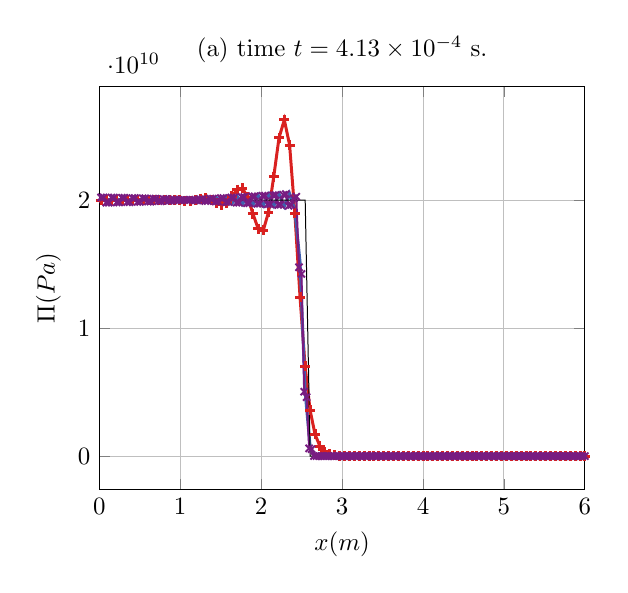
\begin{tikzpicture}[scale=0.9]
\begin{axis}[xlabel=$x (m)$,ylabel=$\Pi (Pa)$,ymajorgrids=true,xmajorgrids=true,legend pos= south west,title={(a) time $t = 4.13\times 10^{-4} $ s.},xmin=0.,xmax=6.]
\addplot[Red,very thick,mark=+,solid] coordinates {(-0.16829522461060809,20007169511.96314) (-0.10369101528636954,19993538918.151154) (-0.03910008978943477,20005752249.60066) (0.025484632606506585,19995780538.002594) (0.09006724602086946,20002982078.92515) (0.1546485608680076,19999277260.36865) (0.2192288029837782,20000480398.382977) (0.2838085169531259,20001789392.278667) (0.3483874448371409,19997301874.53342) (0.41296605184651003,20003008206.491848) (0.4775444471393354,19998613234.28465) (0.5421228879757068,20006614615.093975) (0.6067010779765869,19998205526.77761) (0.6712784021529404,19998711631.528248) (0.7358550513644272,19992106494.35627) (0.8004321132591515,20004770592.319847) (0.8650111473999984,20015779987.73382) (0.9295914037752241,20019625431.191498) (0.9941696099372187,19992929208.032467) (1.0587424231017257,19958300876.966587) (1.123311926789651,19955346446.406406) (1.1878866648233635,20018511640.579197) (1.2524750200748365,20111607980.21578) (1.3170736594252148,20136508388.211338) (1.381663458854595,20010138904.573597) (1.4462219802801475,19778030212.99804) (1.5107477640922773,19635427268.59183) (1.5752752811607438,19797599632.74197) (1.639859880303798,20289327749.506416) (1.70453378203858,20824737676.284462) (1.769262079187512,20916782028.057846) (1.8339384337847504,20225825740.178158) (1.89844144581174,18932646585.446335) (1.9627281077084087,17775081852.48631) (2.026899949421701,17642004813.115726) (2.091185400436795,19055892736.768036) (2.1558364961562164,21827268031.841457) (2.220982442003199,24860462590.307526) (2.286498524038505,26265768115.97021) (2.351967307290947,24295998059.88075) (2.4168137711136564,18956883378.505733) (2.480598163334301,12418144526.81467) (2.543246483139721,7028504053.174823) (2.604999975767945,3579770240.6871147) (2.66618758468537,1694104579.470104) (2.7270670263127124,758612765.168792) (2.7877944080472954,324010645.8165056) (2.848451732493268,132301231.12326287) (2.90907847951511,51629746.688618675) (2.969692513364221,19230481.215198454) (3.0303015063501104,6825460.685392445) (3.0909085945578147,2304741.6481061573) (3.151514997773176,739250.3468689044) (3.212121166898583,224906.37010029136) (3.2727272601131854,64808.36407273517) (3.3333333300016945,17662.648147483887) (3.3939393931074338,4546.039630207806) (3.4545454543493492,1103.2785027445323) (3.5151515151079566,252.0479295361392) (3.5757575757484754,54.104532819766206) (3.6363636363618523,10.890886483248497) (3.69696969696937,2.0511541183492015) (3.7575757575757014,0.36048087591867584) (3.81818181818181,0.05894430243048331) (3.8787878787878776,0.008907404728338756) (3.9393939393939394,0.0011956247957501686) (4.0,0.00011956247957501687) (4.0606060606060606,0.0) (4.121212121212121,0.0) (4.181818181818182,0.0) (4.242424242424242,0.0) (4.303030303030303,0.0) (4.363636363636363,0.0) (4.424242424242425,0.0) (4.484848484848485,0.0) (4.545454545454546,0.0) (4.606060606060606,0.0) (4.666666666666667,0.0) (4.7272727272727275,0.0) (4.787878787878788,0.0) (4.848484848484849,0.0) (4.909090909090909,0.0) (4.96969696969697,0.0) (5.03030303030303,0.0) (5.090909090909091,0.0) (5.151515151515151,0.0) (5.212121212121212,0.0) (5.2727272727272725,0.0) (5.333333333333334,0.0) (5.3939393939393945,0.0) (5.454545454545455,0.0) (5.515151515151516,0.0) (5.575757575757576,0.0) (5.636363636363637,0.0) (5.696969696969697,0.0) (5.757575757575758,0.0) (5.818181818181818,0.0) (5.878787878787879,0.0) (5.9393939393939394,0.0) (6.0,0.0) };
\addplot[Blue,very thick,mark=none,solid] coordinates {(-0.17172662820924992,20126286105.84016) (-0.10660603391933107,19875164406.999718) (-0.04194663943234102,20122512972.128735) (0.022732395165806486,19881553883.263596) (0.08741156754331267,20113695600.0826) (0.15209029604815277,19892923663.406227) (0.21677157984023532,20099953165.28105) (0.2814513737028933,19909115868.450443) (0.3461348221041776,20081472085.12577) (0.4108152742186133,19929906305.25904) (0.4755009353032759,20058503290.3213) (0.5401815288947392,19955007831.504406) (0.6048694507202782,20031358457.677605) (0.6695495822549338,19984074913.32308) (0.7342398618126412,20000405141.87171) (0.7989189035565396,20016709438.584362) (0.8636117080664685,19966060744.260063) (0.9282890378442423,20052467818.751507) (0.9929846146963595,19928785275.12034) (1.0576596352554701,20090869363.82577) (1.1223583072987158,19889072904.409824) (1.1870304528999478,20131405850.072147) (1.2517326020503938,19847442355.372017) (1.3164013359003341,20173552123.78648) (1.3811073800322917,19804426272.137638) (1.4457721874723826,20216777502.470745) (1.5104825561512225,19760559789.583214) (1.575142938446335,20260557805.032604) (1.6398580523466464,19716368448.944717) (1.7045135246263603,20304386827.323605) (1.769233781555915,19672356602.402267) (1.833883876574903,20347788289.080315) (1.8986096450055439,19628995435.82482) (1.96325392193934,20390327196.219734) (2.0279855406761045,19586711664.247425) (2.0926235965346587,20431618631.24346) (2.1573613774425398,19545878506.256725) (2.2219928581092483,20471336442.532116) (2.286737089006318,19506806138.044117) (2.3513616964415003,20505909410.75548) (2.416111827679838,19223361070.797165) (2.4806716443202474,15164119638.328646) (2.544309845123544,4962759374.283854) (2.605921117305293,685282540.4186183) (2.666666666666667,0.0) (2.7272727272727275,0.0) (2.787878787878788,0.0) (2.8484848484848486,0.0) (2.909090909090909,0.0) (2.9696969696969697,0.0) (3.0303030303030303,0.0) (3.090909090909091,0.0) (3.1515151515151514,0.0) (3.2121212121212124,0.0) (3.272727272727273,0.0) (3.3333333333333335,0.0) (3.393939393939394,0.0) (3.4545454545454546,0.0) (3.515151515151515,0.0) (3.5757575757575757,0.0) (3.6363636363636367,0.0) (3.6969696969696972,0.0) (3.757575757575758,0.0) (3.8181818181818183,0.0) (3.878787878787879,0.0) (3.9393939393939394,0.0) (4.0,0.0) (4.0606060606060606,0.0) (4.121212121212121,0.0) (4.181818181818182,0.0) (4.242424242424242,0.0) (4.303030303030303,0.0) (4.363636363636363,0.0) (4.424242424242425,0.0) (4.484848484848485,0.0) (4.545454545454546,0.0) (4.606060606060606,0.0) (4.666666666666667,0.0) (4.7272727272727275,0.0) (4.787878787878788,0.0) (4.848484848484849,0.0) (4.909090909090909,0.0) (4.96969696969697,0.0) (5.03030303030303,0.0) (5.090909090909091,0.0) (5.151515151515151,0.0) (5.212121212121212,0.0) (5.2727272727272725,0.0) (5.333333333333334,0.0) (5.3939393939393945,0.0) (5.454545454545455,0.0) (5.515151515151516,0.0) (5.575757575757576,0.0) (5.636363636363637,0.0) (5.696969696969697,0.0) (5.757575757575758,0.0) (5.818181818181818,0.0) (5.878787878787879,0.0) (5.9393939393939394,0.0) (6.0,0.0) };
\addplot[Purple,thick,mark=x,solid] coordinates {(-0.1708904472675148,19785557608.354362) (-0.141053536291792,19785867406.07991) (-0.10639968665550317,20213101585.682953) (-0.07596722729975139,20213166639.459328) (-0.04207388662674958,19789540452.376034) (-0.011506607675021027,19789557029.70826) (0.022285105176351794,20207044209.230186) (0.052869007707743255,20207022244.274338) (0.08665834628959812,19798347997.174698) (0.1172321822636404,19798342777.723587) (0.151029412846739,20196099111.801785) (0.18158911289003257,20196061786.86517) (0.2154029118177921,19812014870.030228) (0.24594855907990398,19812000299.62603) (0.2797707639479692,20180456497.651028) (0.31030435509337834,20180413575.280464) (0.34414190966292796,19830391975.858875) (0.3746654464197197,19830363703.36432) (0.4085073802039732,20160337163.972836) (0.4390230930475627,20160297191.04402) (0.4728761360608775,19853261920.69269) (0.5033851748227214,19853214144.348965) (0.5372398018663066,20136017953.04032) (0.5677435687389828,20135992244.21921) (0.6016065301582988,19880348866.887726) (0.6321057005127878,19880275931.784782) (0.6659696058844139,20107829473.983624) (0.696465113347797,20107832721.84703) (0.7303345889699686,19911323145.714508) (0.7608267981523694,19911220393.101494) (0.794698155191189,20076150936.708942) (0.8251876402029276,20076201595.577923) (0.8590614435557611,19945806771.791153) (0.8895483774038433,19945671337.662453) (0.9234264348463641,20041403461.894547) (0.9539111397029185,20041524039.151882) (0.9877878427021151,19983380229.063835) (1.0182704154578464,19983211779.396458) (1.0521550389906216,20004041901.242966) (1.0826356465144116,20004259130.529278) (1.1165141722198928,20023590444.9662) (1.146992928994242,20023391823.879498) (1.1808842235337922,19964545222.656155) (1.2113612103069733,19964890116.037624) (1.2452405366181794,20065959588.155254) (1.2757159448575515,20065737455.962234) (1.3096140087494017,19923405655.590446) (1.340087867199397,19923913531.19163) (1.3739668745812406,20109993427.265583) (1.4044394740876944,20109759370.691113) (1.4383442989671855,19881117133.925976) (1.4688156172979114,19881828092.426723) (1.5026930749798657,20155184504.96013) (1.5331634940260768,20154958787.012196) (1.5670749872969294,19838167967.197243) (1.5975444109704615,19839129929.862263) (1.631419066113116,20201034036.189003) (1.6618879405221585,20200860914.39588) (1.695806028986006,19795048344.53005) (1.7262741487880973,19796331467.05578) (1.7601448712991692,20247083731.9241) (1.7906127153916045,20247094549.42775) (1.8245374872621891,19752175452.996067) (1.8550046971339533,19753935406.555477) (1.888870629478351,20292760865.435543) (1.9193376913168196,20293432983.43762) (1.953269542435462,19709654117.014126) (1.9837358641666532,19712407968.009735) (2.0175965864610483,20337138548.75029) (2.048062639992706,20340344997.290543) (2.082002580382462,19666867314.68073) (2.1124672812076257,19672700955.769726) (2.1463232982512577,20378078322.74046) (2.1767870343556104,20391295863.689228) (2.210737854430747,19619814494.093407) (2.241198117559328,19637708700.528072) (2.275052752024238,20408768422.209846) (2.3055096404249302,20461791611.02041) (2.339480401341693,19548900704.7548) (2.3699263513980036,19618213930.10675) (2.4037921787393377,20126713795.32762) (2.4342241255841532,20264753853.55581) (2.468186972434222,14751152292.966133) (2.4985606945703163,14228242465.12349) (2.531508975979028,5032326878.965216) (2.5617596336243342,4603536576.276086) (2.592841768880457,605310239.9535259) (2.623005846412341,539574226.1837834) (2.6532663316582914,0.0005380311580875769) (2.6834170854271355,0.0005380311580875769) (2.7135678391959797,0.0005380311580875769) (2.743718592964824,0.0004782499183000683) (2.7738693467336684,0.0005978123978750856) (2.8040201005025125,0.0005978123978750856) (2.8341708542713566,0.0005380311580875769) (2.8643216080402008,0.0005380311580875769) (2.8944723618090453,0.0005978123978750856) (2.9246231155778895,0.0005978123978750856) (2.9547738693467336,0.0004184686785125597) (2.9849246231155777,0.0003586874387250511) (3.015075376884422,0.0004782499183000683) (3.0452261306532664,0.0004184686785125597) (3.0753768844221105,0.0003586874387250511) (3.1055276381909547,0.0003586874387250511) (3.135678391959799,0.0005380311580875769) (3.165829145728643,0.0005380311580875769) (3.1959798994974875,0.0004184686785125597) (3.2261306532663316,0.0004184686785125597) (3.2562814070351758,0.0004782499183000683) (3.28643216080402,0.0004184686785125597) (3.316582914572864,0.0004782499183000683) (3.3467336683417086,0.0004184686785125597) (3.3768844221105527,0.0004184686785125597) (3.407035175879397,0.0003586874387250511) (3.437185929648241,0.0003586874387250511) (3.467336683417085,0.0003586874387250511) (3.4974874371859297,0.0003586874387250511) (3.527638190954774,0.0003586874387250511) (3.557788944723618,0.0003586874387250511) (3.587939698492462,0.0003586874387250511) (3.618090452261306,0.0003586874387250511) (3.648241206030151,0.0003586874387250511) (3.678391959798995,0.0002989061989375425) (3.708542713567839,0.0002989061989375425) (3.738693467336683,0.0004184686785125597) (3.7688442211055273,0.0004184686785125597) (3.798994974874372,0.0003586874387250511) (3.829145728643216,0.0003586874387250511) (3.85929648241206,0.0001793437193625254) (3.8894472361809043,0.0001793437193625254) (3.9195979899497484,0.0001793437193625254) (3.949748743718593,0.00011956247957501691) (3.979899497487437,0.0003586874387250511) (4.010050251256281,0.0002989061989375425) (4.040201005025126,0.0002989061989375425) (4.0703517587939695,0.0002989061989375425) (4.100502512562814,0.00023912495915003393) (4.130653266331658,0.0003586874387250511) (4.160804020100502,0.0003586874387250511) (4.190954773869347,0.0003586874387250511) (4.221105527638191,0.0003586874387250511) (4.251256281407035,0.0003586874387250511) (4.281407035175879,0.0003586874387250511) (4.311557788944723,0.0003586874387250511) (4.341708542713568,0.0002989061989375425) (4.371859296482412,0.0002989061989375425) (4.402010050251256,0.00023912495915003393) (4.4321608040201,0.00023912495915003393) (4.4623115577889445,0.00023912495915003393) (4.492462311557789,0.00023912495915003393) (4.522613065326633,0.0002989061989375425) (4.552763819095477,0.0002989061989375425) (4.582914572864321,0.0002989061989375425) (4.613065326633166,0.00023912495915003393) (4.64321608040201,0.0003586874387250511) (4.673366834170854,0.0003586874387250511) (4.703517587939698,0.0002989061989375425) (4.733668341708542,0.00023912495915003393) (4.763819095477387,0.0002989061989375425) (4.793969849246231,0.0002989061989375425) (4.824120603015075,0.0002989061989375425) (4.8542713567839195,0.0002989061989375425) (4.884422110552763,0.0003586874387250511) (4.914572864321608,0.0003586874387250511) (4.944723618090452,0.00023912495915003393) (4.974874371859296,0.00023912495915003393) (5.005025125628141,0.0003586874387250511) (5.035175879396984,0.0002989061989375425) (5.065326633165829,0.0002989061989375425) (5.0954773869346734,0.0002989061989375425) (5.125628140703517,0.00023912495915003393) (5.155778894472362,0.0002989061989375425) (5.185929648241205,0.0003586874387250511) (5.21608040201005,0.0003586874387250511) (5.2462311557788945,0.0001793437193625254) (5.276381909547738,0.0001793437193625254) (5.306532663316583,0.0002989061989375425) (5.3366834170854265,0.00023912495915003393) (5.366834170854271,0.00023912495915003393) (5.396984924623116,0.00023912495915003393) (5.427135678391959,0.00023912495915003393) (5.457286432160804,0.00023912495915003393) (5.487437185929648,0.0001793437193625254) (5.517587939698492,0.00011956247957501691) (5.547738693467337,5.978123978750844e-05) (5.57788944723618,5.978123978750844e-05) (5.608040201005025,0.0001793437193625254) (5.638190954773869,0.0001793437193625254) (5.668341708542713,0.00023912495915003393) (5.698492462311558,0.0001793437193625254) (5.7286432160804015,0.00011956247957501691) (5.758793969849246,5.978123978750844e-05) (5.788944723618091,0.00011956247957501691) (5.819095477386934,5.978123978750844e-05) (5.849246231155779,0.0) (5.879396984924623,0.0) (5.909547738693467,0.0) (5.939698492462312,5.978123978750844e-05) (5.969849246231155,-0.0001195624795750168) (6.0,0.0) };
\addplot[black,thin,mark=none,solid] coordinates {(-0.17172662820924992,19999999999.999966) (-0.10660603391933107,19999999999.999966) (-0.04194663943234102,19999999999.999966) (0.022732395165806486,19999999999.999966) (0.08741156754331267,19999999999.999966) (0.15209029604815277,19999999999.999966) (0.21677157984023532,19999999999.999966) (0.2814513737028933,19999999999.999966) (0.3461348221041776,19999999999.999966) (0.4108152742186133,19999999999.999966) (0.4755009353032759,19999999999.999966) (0.5401815288947392,19999999999.999966) (0.6048694507202782,19999999999.999966) (0.6695495822549338,19999999999.999966) (0.7342398618126412,19999999999.999966) (0.7989189035565396,19999999999.999966) (0.8636117080664685,19999999999.999966) (0.9282890378442423,19999999999.999966) (0.9929846146963595,19999999999.999966) (1.0576596352554701,19999999999.999966) (1.1223583072987158,19999999999.999966) (1.1870304528999478,19999999999.999966) (1.2517326020503938,19999999999.999966) (1.3164013359003341,19999999999.999966) (1.3811073800322917,19999999999.999966) (1.4457721874723826,19999999999.999966) (1.5104825561512225,19999999999.999966) (1.575142938446335,19999999999.999966) (1.6398580523466464,19999999999.999966) (1.7045135246263603,19999999999.999966) (1.769233781555915,19999999999.999966) (1.833883876574903,19999999999.999966) (1.8986096450055439,19999999999.999966) (1.96325392193934,19999999999.999966) (2.0279855406761045,19999999999.999966) (2.0926235965346587,19999999999.999966) (2.1573613774425398,19999999999.999966) (2.2219928581092483,19999999999.999966) (2.286737089006318,19999999999.999966) (2.3513616964415003,19999999999.999966) (2.416111827679838,19999999999.999966) (2.4806716443202474,19999999999.999966) (2.544309845123544,19999999999.999966) (2.605921117305293,0.0) (2.666666666666667,0.0) (2.7272727272727275,0.0) (2.787878787878788,0.0) (2.8484848484848486,0.0) (2.909090909090909,0.0) (2.9696969696969697,0.0) (3.0303030303030303,0.0) (3.090909090909091,0.0) (3.1515151515151514,0.0) (3.2121212121212124,0.0) (3.272727272727273,0.0) (3.3333333333333335,0.0) (3.393939393939394,0.0) (3.4545454545454546,0.0) (3.515151515151515,0.0) (3.5757575757575757,0.0) (3.6363636363636367,0.0) (3.6969696969696972,0.0) (3.757575757575758,0.0) (3.8181818181818183,0.0) (3.878787878787879,0.0) (3.9393939393939394,0.0) (4.0,0.0) (4.0606060606060606,0.0) (4.121212121212121,0.0) (4.181818181818182,0.0) (4.242424242424242,0.0) (4.303030303030303,0.0) (4.363636363636363,0.0) (4.424242424242425,0.0) (4.484848484848485,0.0) (4.545454545454546,0.0) (4.606060606060606,0.0) (4.666666666666667,0.0) (4.7272727272727275,0.0) (4.787878787878788,0.0) (4.848484848484849,0.0) (4.909090909090909,0.0) (4.96969696969697,0.0) (5.03030303030303,0.0) (5.090909090909091,0.0) (5.151515151515151,0.0) (5.212121212121212,0.0) (5.2727272727272725,0.0) (5.333333333333334,0.0) (5.3939393939393945,0.0) (5.454545454545455,0.0) (5.515151515151516,0.0) (5.575757575757576,0.0) (5.636363636363637,0.0) (5.696969696969697,0.0) (5.757575757575758,0.0) (5.818181818181818,0.0) (5.878787878787879,0.0) (5.9393939393939394,0.0) (6.0,0.0) };
%\legend{mpm,dgmpm,dgmpm 2ppc (RK2),exact}
\end{axis}
\end{tikzpicture}
%%% Local Variables:
%%% mode: latex
%%% TeX-master: "../../mainManuscript"
%%% End:
}
%   {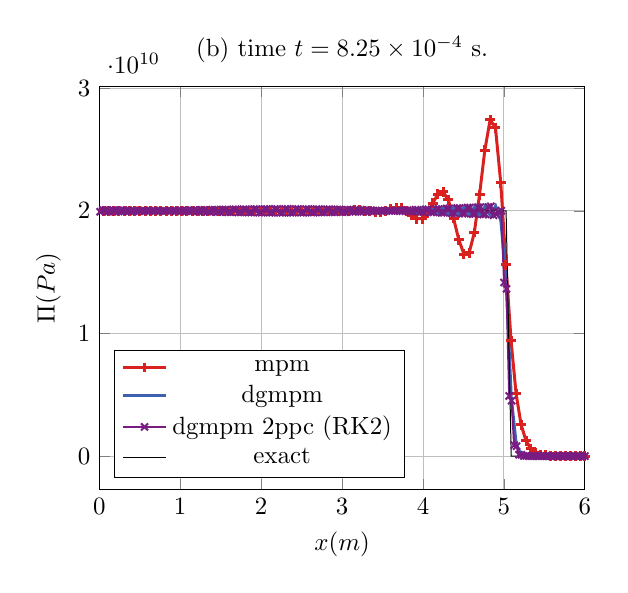
\begin{tikzpicture}[scale=0.9]
\begin{axis}[xlabel=$x (m)$,ylabel=$\Pi (Pa)$,ymajorgrids=true,xmajorgrids=true,legend pos= south west,title={(b) time $t = 8.25\times 10^{-4} $ s.},xmin=0.,xmax=6.]
\addplot[Red,very thick,mark=+,solid] coordinates {(-0.3373970335129395,20002444911.789238) (-0.2727928966297102,19997432693.913857) (-0.20820196231046736,20001959247.078884) (-0.14361740752040095,19997652072.059658) (-0.0790347885190633,20001174478.201954) (-0.014453732919982308,19998113117.396988) (0.050126384917715185,20000219977.304207) (0.1147058039394095,19998668866.378258) (0.17928462960154493,19999250601.410038) (0.24386307172432597,19999169326.347557) (0.30844111377254735,19998402881.7715) (0.3730189157030712,19999501047.64978) (0.43759644654074153,19997762967.548557) (0.50217381047918,19999609942.781967) (0.5667509959420945,19997354773.840668) (0.6313280560675543,19999501477.373802) (0.6959050053014575,19997148374.83382) (0.7604818569685504,19999225474.73323) (0.8250586461934166,19997083680.145477) (0.8896353603808954,19998851023.15548) (0.9542120453300287,19997089910.935226) (1.0187886757648426,19998440828.306694) (1.083365299089184,19997111161.46065) (1.1479418881286723,19998051169.644836) (1.2125184850646817,19997116278.583233) (1.2770950657270574,19997699692.89216) (1.3416716627444705,19997067231.472904) (1.406248258920999,19997388896.74777) (1.4708248806644153,19997000578.277737) (1.535401519422826,19997171020.844025) (1.599978191235337,19996918101.970993) (1.6645548853210443,19996920744.490818) (1.7291316080867047,19996700814.432293) (1.7937083617143608,19996691407.553604) (1.8582851678967984,19996686120.493286) (1.9228620377138623,19996772465.623905) (1.9874389634593603,19996650100.204838) (2.0520159097351134,19996304228.832874) (2.1165928542213344,19995901639.208565) (2.181169830867098,19995922422.124294) (2.245746933014004,19996569013.601753) (2.3103242301117346,19997366737.300365) (2.3749016574282744,19997253707.766594) (2.439479003437918,19995610575.776176) (2.50405608348629,19993366031.355854) (2.5686330012527394,19992897527.09602) (2.633210227393201,19996035016.03268) (2.6977882771955914,20001461417.7394) (2.7623671197745874,20004234447.067886) (2.826945847657703,19999248815.338493) (2.891523147056034,19986954084.876858) (2.9560985175931442,19976226893.658413) (3.020673338478683,19979732556.833313) (3.0852505531422554,20002734650.377262) (3.149832540815079,20033514677.442947) (3.2144183646554727,20045779859.54768) (3.279002790793957,20016543982.692215) (3.343578922732655,19949761640.288918) (3.408143766461,19886271903.166637) (3.472703046370895,19885090545.547707) (3.5372706584700393,19980762153.863453) (3.6018608542803987,20143069670.253544) (3.666476517033703,20272160418.98628) (3.731101311045297,20247014960.951336) (3.7957034722589915,20011400843.260548) (3.8602530814356824,19644164431.403908) (3.924745093767238,19352701051.419342) (3.9892134274545104,19373330976.866657) (4.0537234224180505,19827324507.865147) (4.118341053895788,20606668355.762043) (4.183090744717796,21350802856.75598) (4.247923050028822,21564506017.293846) (4.312715450250743,20887275093.29332) (4.37731903294961,19390073952.106243) (4.441637416097922,17648045449.929543) (4.505695564266106,16477972514.036726) (4.569656065119688,16564993555.823458) (4.633774257438693,18234485218.06143) (4.698311215790016,21316982189.19614) (4.763422276660747,24943663529.441895) (4.829040675663493,27423065710.3382) (4.894809718237837,26786511205.121754) (4.960153433745974,22304704037.851227) (5.024529459659876,15612866271.729282) (5.0877165905602455,9395941456.960642) (5.149868001086729,5080803829.979227) (5.211310703936358,2571948063.5769763) (5.2723407989116975,1251943821.049851) (5.333153160181875,594362859.6955562) (5.393856948062081,276921639.57925117) (5.454508383498881,126868092.89648758) (5.515135140653742,57148823.407327816) (5.575750476779182,25288021.07216049) (5.636360618733436,10978518.189306797) (5.696968440582231,4670443.034755671) (5.757575245750145,1944881.6231991085) (5.818181614449599,792440.4555923982) (5.878787799930788,317032.1081128554) (5.939393910671728,128397.83825474144) (5.9999999928647405,63394.068050559574) };
\addplot[Blue,very thick,mark=none,solid] coordinates {(-0.34300326824190164,19867161670.92257) (-0.27788319029024855,20132353190.445465) (-0.21322278871058642,19869130721.386837) (-0.14854524891661086,20129142425.138195) (-0.08386416618006085,19873652842.561867) (-0.01918775421833607,20123421266.062355) (0.04549613686190245,19880628150.922165) (0.11017305016981589,20115318727.80989) (0.17485949985090674,19889901681.750263) (0.2395368602373047,20105017064.568512) (0.30422552430806427,19901266649.63073) (0.36890325481559005,20092747885.067688) (0.43359370903377453,19914468812.52206) (0.4982717227365738,20078787280.255478) (0.5629635229582883,19929211827.51738) (0.6276417735241854,20063450128.705578) (0.6923344895943412,19945162699.15721) (0.7570129870707453,20047081201.542427) (0.8217062271247281,19961961586.06754) (0.8863850430702915,20030053095.45937) (0.9510784635094146,19979226355.574352) (1.015757722065038,20012756186.25665) (1.0804510262905567,19996560201.361286) (1.1451308857252085,19995591078.27326) (1.2098238162869241,20013559902.98507) (1.2745044463948634,19978961181.23721) (1.339196775641803,20029823630.182865) (1.40387833619713,19963265075.256836) (1.468569859873193,20044958518.655983) (1.533252484114899,19948889080.898514) (1.5979430206134242,20058587899.768158) (1.6626268056632443,19936200167.451828) (1.7273162014193637,20070358058.719982) (1.7920012052713876,19925539314.253044) (1.8566893446755617,20079944419.1636) (1.9213755875853589,19917215422.042995) (1.9860624044406507,20087057076.01931) (2.0507498716789403,19911499852.8977) (2.115435358948472,20091445622.53556) (2.1801240021419153,19908621665.315594) (2.244808217516759,20092903240.062386) (2.3094979529589694,19908763592.066013) (2.3741810192336423,20091270026.991108) (2.4388717231008803,19912058799.92498) (2.503553823894505,20086435560.409016) (2.568245325654722,19918588470.128216) (2.6329266981213357,20078340688.316597) (2.6976187741402335,19928380238.783928) (2.762299700805929,20066978548.729008) (2.826992075723227,19941407541.779408) (2.891672923066381,20052394804.467094) (2.956365346939235,19957589915.641735) (3.0210465161215225,20034687069.70895) (3.0857385707248404,19976794311.40647) (3.150420408966768,20014003488.348423) (3.2151116547381915,19998837479.325516) (3.279794587709358,19990540408.2874) (3.3444845724109693,20023489474.801964) (3.4091690555988876,19964539084.58109) (3.4738573026283968,20050478317.273846) (3.5385438113443364,19936281343.307373) (3.6032298274016155,20079495802.060196) (3.667918848609329,19906084152.544304) (3.732602130509684,20110204420.136734) (3.7972941529817468,19874293081.001152) (3.8619741937006657,20142245283.97256) (3.926669697644514,19841274680.052853) (3.9913459924348733,20175246892.79887) (4.056045440000399,19807407898.849144) (4.120717493458492,20208834504.42018) (4.185421321345374,19773074740.97144) (4.250088655916392,20242639943.665905) (4.314797270727306,19738650272.25273) (4.379459436438253,20276310806.877926) (4.44417321250515,19704493074.44567) (4.508829797148642,20309519959.73904) (4.573549076088961,19670935330.734615) (4.638199714390607,20341974420.673492) (4.702924805180256,19638273500.285717) (4.767569185544008,20373421858.440434) (4.832300363715842,19606757017.834343) (4.896938230755509,20398348853.4957) (4.961674477599282,19194568925.629593) (5.026219132132484,14312041520.443619) (5.089697845458756,4819432981.92643) (5.151288275508455,961012171.3536986) (5.212092547900456,129265691.8128923) (5.272725221999611,10032930.422299773) (5.333333333333334,0.0) (5.3939393939393945,0.0) (5.454545454545455,0.0) (5.515151515151516,0.0) (5.575757575757576,0.0) (5.636363636363637,0.0) (5.696969696969697,0.0) (5.757575757575758,0.0) (5.818181818181818,0.0) (5.878787878787879,0.0) (5.9393939393939394,0.0) (6.0,0.0) };
\addplot[Purple,thick,mark=x,solid] coordinates {(-0.3413421216005564,20084454120.70626) (-0.3115046323967783,20084503231.20538) (-0.2768503231825786,19916185104.896652) (-0.24641699137696205,19916224025.277943) (-0.21252704225382044,20082521029.067745) (-0.18195851890502224,20082494630.53035) (-0.14816447224841806,19919503737.228157) (-0.11757957066435366,19919560593.514977) (-0.08379589265784985,20077952554.12534) (-0.05322085703338879,20077898893.370735) (-0.019419148715127472,19925390458.555717) (0.011141460181846741,19925475541.195904) (0.04494772591031657,20070870972.704773) (0.07549443808768144,20070794153.22469) (0.10932301412763686,19933726420.88046) (0.13985737952332528,19933837024.581604) (0.173685926639547,20061431321.92105) (0.20421035859246994,20061332816.082695) (0.23806014963800134,19944334708.452976) (0.2685764825007371,19944466366.306778) (0.3024195284182063,20049838277.438824) (0.33292927588669197,20049719936.704403) (0.3667927137931127,19956995564.425697) (0.39729694359154255,19957143051.16299) (0.43114948448894214,20036346157.64271) (0.4616491777370185,20036210511.364494) (0.49552220217347964,19971448924.99579) (0.5260180299294327,19971606591.563793) (0.5598772972948788,20021247143.683044) (0.5903698622131245,20021097455.275764) (0.624249900829884,19987369347.34896) (0.654739595219531,19987531478.95478) (0.6886040890282352,20004870125.83432) (0.7190912475113203,20004710463.922737) (0.7529767194177145,20004410302.615177) (0.7834615704641484,20004571380.654194) (0.8173305879064932,19987574487.067276) (0.847813305881258,19987409722.84234) (0.8817031821057704,20022200269.99343) (0.9121839339935235,20022355214.726463) (0.9460571483764127,19969742299.809765) (0.9765360354593392,19969578036.0323) (1.0104294819309994,20040348503.200268) (1.040906682974281,20040492861.37563) (1.0747838335358735,19951770413.041492) (1.105259430932844,19951612839.252544) (1.1391555845596315,20058452407.676346) (1.1696298054671987,20058582471.461685) (1.2035105315252492,19934062461.007298) (1.2339834581168863,19933918134.766502) (1.26788134906568,20076105339.2744) (1.2983532590129288,20076218192.12232) (1.332237072733504,19917020987.71109) (1.3627080375199254,19916896548.399593) (1.3966066343017862,20092904393.807842) (1.4270769595734558,20092997886.904884) (1.4609633199405618,19901039886.204426) (1.4914330391974988,19900941714.78726) (1.5253313681450775,20108457966.61612) (1.5558007815742427,20108530636.852116) (1.58968921499868,19886497320.08024) (1.620158288063799,19886431164.442165) (1.6540555703547062,20122392933.588875) (1.6845245667812516,20122443880.233562) (1.7184147802161702,19873749252.240623) (1.7488835761357309,19873719842.724926) (1.7827793345331566,20134361342.940174) (1.8132481375124534,20134390084.955162) (1.8471400866548187,19863123660.159065) (1.8776086764287256,19863134343.309586) (1.9115027873522425,20144046533.93617) (1.941971308324001,20144052872.731007) (1.9758652132489007,19854915473.262917) (2.00633335571715,19854967893.19228) (2.040226079745077,20151168618.87888) (2.070693985199334,20151152531.999393) (2.104590384682496,19849382232.053566) (2.135057901533144,19849476088.127354) (2.1689496169030114,20155489277.933567) (2.199417036193448,20155450867.5519) (2.2333157795929726,19846740444.56689) (2.263782879164934,19846873351.154137) (2.29767330438176,20156815822.998478) (2.328140263166214,20156755339.15534) (2.3620411522751077,19847162606.42877) (2.392507699460935,19847330075.36992) (2.426397066000551,20155004487.461292) (2.456863380789038,20154922439.98095) (2.4907664359543715,19850774856.538464) (2.5212322666486426,19850970415.948395) (2.555120899476285,20149962895.29097) (2.585586439450331,20149860260.53971) (2.6194915665074547,19857655259.362076) (2.649956589833981,19857870713.761578) (2.6838448104013497,20141651656.730064) (2.7143095156589245,20141530176.422417) (2.7482165060193036,19867832720.558792) (2.7786806902628784,19868058547.559307) (2.8125688393803885,20130084962.0052) (2.8430326926994947,20129947521.903427) (2.8769412584352323,19881286508.15238) (2.907404596472946,19881512377.22646) (2.9412930658856,20115330328.24148) (2.9717560576395274,20115181396.04708) (3.0056658655431305,19897946940.899014) (3.036128344041352,19898162329.4085) (3.070017595121079,20097507428.18806) (3.100479700762355,20097353520.394882) (3.1343903886946634,19917696528.872005) (3.164851976527314,19917891402.385876) (3.1987425343389657,20076785327.117977) (3.2292037151467032,20076635470.893406) (3.2631148843368862,19940372025.717415) (3.29357554543851,19940537544.133724) (3.3274679679788997,20053378728.587624) (3.357928194540636,20053244881.13022) (3.3918393831412645,19965767607.411438) (3.422299107793317,19965896815.490192) (3.456193940921393,20027543050.174908) (3.486653228633958,20027440439.6467) (3.520563880585621,19993639102.67711) (3.5510227208761473,19993727568.79394) (3.5849204556914755,19999568290.3942) (3.615378895931043,19999515651.498085) (3.649288342283673,20023709203.216496) (3.6797464349135187,20023755595.7377) (3.7136474841959903,19969771717.557053) (3.744105255467703,19969791423.13771) (3.7780127218729365,20055673406.51396) (3.8084702852479175,20055680096.82016) (3.8423749893302808,19938489456.48) (3.8728323391771236,19938607645.218704) (3.906736984687898,20089205875.665604) (3.9371942857875872,20089180050.754776) (3.971102948275359,19906067025.556553) (4.001560146502916,19906314216.038258) (4.035461128102997,20123961775.83972) (4.065918424699022,20123919131.594395) (4.099831368443375,19872848196.356743) (4.130288641421362,19873262528.891777) (4.164185191417915,20159573473.009506) (4.194642662567189,20159553030.56887) (4.228560290996899,19839166473.88708) (4.259017750563116,19839808941.31075) (4.292909258187191,20195675341.985744) (4.323366935108609,20195799856.708904) (4.357289795589992,19805336038.508987) (4.387747366655722,19806358551.373158) (4.421633460585793,20231834709.36628) (4.452091150023708,20232554202.447742) (4.48602003137047,19771483196.513275) (4.516477347673006,19773429826.418495) (4.5503580637774,20267126470.97277) (4.58081526693636,20270193617.440983) (4.614751454576072,19736918846.87252) (4.645207821787056,19742059913.02803) (4.679083775444953,20298852761.491997) (4.7095395048223025,20311197166.66586) (4.743485099523246,19697906198.47693) (4.773938201390833,19716155926.428547) (4.807812253028679,20317459432.2131) (4.838261988618075,20366464115.49615) (4.872224665961511,19636335499.984386) (4.9026646932738345,19711246044.137264) (4.936550533899874,19912517877.28153) (4.966975247749498,20015432325.29268) (5.000903022698816,14157492462.311962) (5.031270011791101,13637448020.679394) (5.064107380705877,4900151134.711801) (5.094355634519364,4518545375.67135) (5.125418372928627,896010785.5143551) (5.1555887970834,812792584.0059679) (5.1859044083527275,115327096.28225213) (5.21605773200199,103644640.31290346) (5.246229541628463,7935027.787381989) (5.276380471907977,7067282.007803429) (5.306532663316583,0.0004782499183000683) (5.3366834170854265,0.0005978123978750856) (5.366834170854271,0.0004782499183000683) (5.396984924623116,0.0004782499183000683) (5.427135678391959,0.0004782499183000683) (5.457286432160804,0.0005380311580875769) (5.487437185929648,0.0005380311580875769) (5.517587939698492,0.0004782499183000683) (5.547738693467337,0.0005978123978750856) (5.57788944723618,0.0005978123978750856) (5.608040201005025,0.0005380311580875769) (5.638190954773869,0.0005380311580875769) (5.668341708542713,0.0005380311580875769) (5.698492462311558,0.0005380311580875769) (5.7286432160804015,0.0003586874387250511) (5.758793969849246,0.0002989061989375425) (5.788944723618091,0.0005380311580875769) (5.819095477386934,0.0004782499183000683) (5.849246231155779,0.0004184686785125597) (5.879396984924623,0.0004184686785125597) (5.909547738693467,0.0004782499183000683) (5.939698492462312,0.0004782499183000683) (5.969849246231155,0.0001793437193625254) (6.0,0.00023912495915003393) };
\addplot[black,thin,mark=none,solid] coordinates {(-0.34300326824190164,19999999999.999966) (-0.27788319029024855,19999999999.999966) (-0.21322278871058642,19999999999.999966) (-0.14854524891661086,19999999999.999966) (-0.08386416618006085,19999999999.999966) (-0.01918775421833607,19999999999.999966) (0.04549613686190245,19999999999.999966) (0.11017305016981589,19999999999.999966) (0.17485949985090674,19999999999.999966) (0.2395368602373047,19999999999.999966) (0.30422552430806427,19999999999.999966) (0.36890325481559005,19999999999.999966) (0.43359370903377453,19999999999.999966) (0.4982717227365738,19999999999.999966) (0.5629635229582883,19999999999.999966) (0.6276417735241854,19999999999.999966) (0.6923344895943412,19999999999.999966) (0.7570129870707453,19999999999.999966) (0.8217062271247281,19999999999.999966) (0.8863850430702915,19999999999.999966) (0.9510784635094146,19999999999.999966) (1.015757722065038,19999999999.999966) (1.0804510262905567,19999999999.999966) (1.1451308857252085,19999999999.999966) (1.2098238162869241,19999999999.999966) (1.2745044463948634,19999999999.999966) (1.339196775641803,19999999999.999966) (1.40387833619713,19999999999.999966) (1.468569859873193,19999999999.999966) (1.533252484114899,19999999999.999966) (1.5979430206134242,19999999999.999966) (1.6626268056632443,19999999999.999966) (1.7273162014193637,19999999999.999966) (1.7920012052713876,19999999999.999966) (1.8566893446755617,19999999999.999966) (1.9213755875853589,19999999999.999966) (1.9860624044406507,19999999999.999966) (2.0507498716789403,19999999999.999966) (2.115435358948472,19999999999.999966) (2.1801240021419153,19999999999.999966) (2.244808217516759,19999999999.999966) (2.3094979529589694,19999999999.999966) (2.3741810192336423,19999999999.999966) (2.4388717231008803,19999999999.999966) (2.503553823894505,19999999999.999966) (2.568245325654722,19999999999.999966) (2.6329266981213357,19999999999.999966) (2.6976187741402335,19999999999.999966) (2.762299700805929,19999999999.999966) (2.826992075723227,19999999999.999966) (2.891672923066381,19999999999.999966) (2.956365346939235,19999999999.999966) (3.0210465161215225,19999999999.999966) (3.0857385707248404,19999999999.999966) (3.150420408966768,19999999999.999966) (3.2151116547381915,19999999999.999966) (3.279794587709358,19999999999.999966) (3.3444845724109693,19999999999.999966) (3.4091690555988876,19999999999.999966) (3.4738573026283968,19999999999.999966) (3.5385438113443364,19999999999.999966) (3.6032298274016155,19999999999.999966) (3.667918848609329,19999999999.999966) (3.732602130509684,19999999999.999966) (3.7972941529817468,19999999999.999966) (3.8619741937006657,19999999999.999966) (3.926669697644514,19999999999.999966) (3.9913459924348733,19999999999.999966) (4.056045440000399,19999999999.999966) (4.120717493458492,19999999999.999966) (4.185421321345374,19999999999.999966) (4.250088655916392,19999999999.999966) (4.314797270727306,19999999999.999966) (4.379459436438253,19999999999.999966) (4.44417321250515,19999999999.999966) (4.508829797148642,19999999999.999966) (4.573549076088961,19999999999.999966) (4.638199714390607,19999999999.999966) (4.702924805180256,19999999999.999966) (4.767569185544008,19999999999.999966) (4.832300363715842,19999999999.999966) (4.896938230755509,19999999999.999966) (4.961674477599282,19999999999.999966) (5.026219132132484,19999999999.999966) (5.089697845458756,0.0) (5.151288275508455,0.0) (5.212092547900456,0.0) (5.272725221999611,0.0) (5.333333333333334,0.0) (5.3939393939393945,0.0) (5.454545454545455,0.0) (5.515151515151516,0.0) (5.575757575757576,0.0) (5.636363636363637,0.0) (5.696969696969697,0.0) (5.757575757575758,0.0) (5.818181818181818,0.0) (5.878787878787879,0.0) (5.9393939393939394,0.0) (6.0,0.0) };
\legend{mpm,dgmpm,dgmpm 2ppc (RK2),exact}
\end{axis}
\end{tikzpicture}
%%% Local Variables:
%%% mode: latex
%%% TeX-master: "../../mainManuscript"
%%% End:
}
%   \caption{shock stress $50\sigma^y$}
%   \label{fig:he_shock}
% \end{figure}
% \begin{figure}[h!]
%   \centering
%   {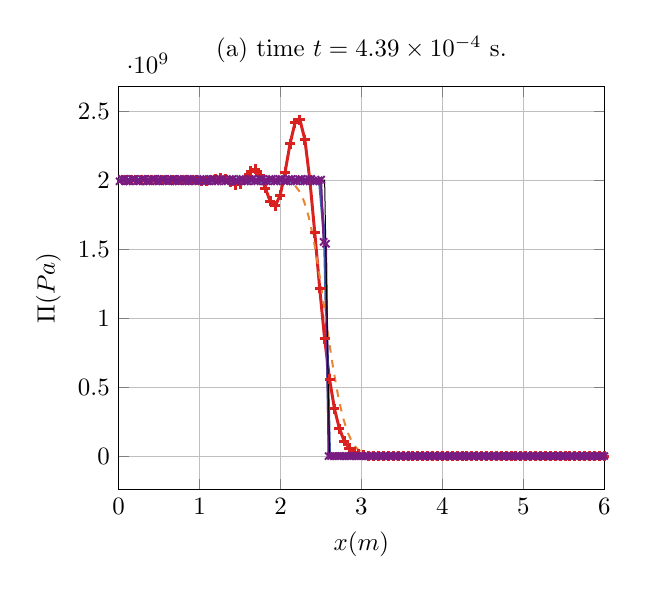
\begin{tikzpicture}[scale=0.9]
\begin{axis}[xlabel=$x (m)$,ylabel=$\Pi (Pa)$,ymajorgrids=true,xmajorgrids=true,legend pos= south west,title={(a) time $t = 4.39\times 10^{-4} $ s.},xmin=0.,xmax=6.]
\addplot[Red,very thick,mark=+,solid] coordinates {(-0.01889090575892736,2000726227.9548469) (0.04215938121847631,1999333692.2170322) (0.10320950300088187,2000564307.210718) (0.1642595721497595,1999551619.5161746) (0.22530959528412595,2000366086.7014122) (0.2863596365377364,1999918681.081198) (0.34740962154368255,1999967513.1983385) (0.4084596019243027,1999982956.3759255) (0.4695095542813397,1999789300.767052) (0.5305595706356425,2000638143.0446692) (0.5916096101001108,2000058185.8142667) (0.6526595840065709,2000089500.8199706) (0.7137094080712463,1998731982.696904) (0.7747591964204517,1999802718.761434) (0.8358092400792819,2001103352.5160503) (0.8968596075653851,2002797653.0377228) (0.9579099107745452,2000545034.2858593) (1.0189595027783396,1996318945.1727874) (1.0800083591701581,1993841183.3513687) (1.1410574970379839,1998917122.885443) (1.2021083083094746,2009171450.4722426) (1.2631608670075336,2014924382.2673836) (1.324213039463032,2005656899.5451016) (1.385261769152474,1983449039.423849) (1.4463061626617941,1966015537.327388) (1.507349635271763,1975043578.4303389) (1.5683984989928055,2015342835.6991093) (1.6294570537824011,2063738687.704247) (1.6905226695860884,2079996363.0337298) (1.7515852284367635,2035769364.3281224) (1.8126325838500514,1940918000.2995517) (1.8736591534269504,1845811486.1301281) (1.9346719362907874,1815039899.0369656) (1.9956894703716108,1889210362.9092839) (2.0567336535453324,2058642788.6612728) (2.117818634233786,2262898814.531011) (2.178942416069636,2414862117.653746) (2.240085148148831,2437155605.434466) (2.301214705448431,2293758990.699916) (2.3622968082809916,2001786574.9585006) (2.4233050712621194,1618923825.3431814) (2.4842269247483553,1216053195.9451652) (2.5450639204752132,851463994.3153192) (2.605827780198291,557925039.8409315) (2.66653493894023,343357124.31856114) (2.7272019233986486,199050644.20604298) (2.7878426090238304,108945510.80319592) (2.8484672666547697,56388618.61462657) (2.9090827809076343,27631268.92148142) (2.9696933946574,12828198.479249047) (3.030301534387653,5645398.76980634) (3.0909084955126,2355626.776140429) (3.15151492615744,932070.1392538762) (3.212121131032279,349709.3400203979) (3.2727272450009446,124397.82639027077) (3.333333324329144,41941.30302034219) (3.3939393911637925,13397.315005244573) (3.4545454537338864,4052.370067713768) (3.515151514926613,1159.9211676619566) (3.5757575756985602,313.92767018390856) (3.6363636363489893,80.26085778895391) (3.6969696969662627,19.36314356717398) (3.7575757575749984,4.402469841671484) (3.8181818181816607,0.9419729953317703) (3.878787878787848,0.1893869676468267) (3.9393939393939337,0.03568940015314253) (3.999999999999999,0.006277030177688385) (4.0606060606060606,0.0010162810763876433) (4.121212121212121,0.00011956247957501687) (4.181818181818182,0.0) (4.242424242424242,0.0) (4.303030303030303,0.0) (4.363636363636363,0.0) (4.424242424242425,0.0) (4.484848484848485,0.0) (4.545454545454546,0.0) (4.606060606060606,0.0) (4.666666666666667,0.0) (4.7272727272727275,0.0) (4.787878787878788,0.0) (4.848484848484849,0.0) (4.909090909090909,0.0) (4.96969696969697,0.0) (5.03030303030303,0.0) (5.090909090909091,0.0) (5.151515151515151,0.0) (5.212121212121212,0.0) (5.2727272727272725,0.0) (5.333333333333334,0.0) (5.3939393939393945,0.0) (5.454545454545455,0.0) (5.515151515151516,0.0) (5.575757575757576,0.0) (5.636363636363637,0.0) (5.696969696969697,0.0) (5.757575757575758,0.0) (5.818181818181818,0.0) (5.878787878787879,0.0) (5.9393939393939394,0.0) (6.0,0.0) };
\addplot[Blue,very thick,mark=none,solid] coordinates {(-0.01905005116856936,2008739016.0347507) (0.04200625800028209,1991261736.4427555) (0.10305754928183601,2008739100.409834) (0.16410893267859902,1991261521.605884) (0.22516022487211998,2008739334.4376273) (0.28621163420310985,1991261157.0218182) (0.3472629006887729,2008739718.3484042) (0.40831433629779745,1991260642.4918854) (0.4693655770844152,2008740252.4789007) (0.5304170389659988,1991259977.710147) (0.591468254064157,2008740937.273132) (0.6525197422102871,1991259162.2632153) (0.713570931632428,2008741773.281487) (0.7746224460325223,1991258195.6316195) (0.8356736097927291,2008742761.1610267) (0.8967251504336042,1991257077.1895308) (0.9577762885477589,2008743901.6730618) (1.0188278554137018,1991255806.2060382) (1.0798789678994447,2008745195.6865165) (1.1409305609721991,1991254381.844086) (1.2019816478489238,2008746644.1731992) (1.2630332671077074,1991252803.1625357) (1.3240843283965613,2008748248.2084675) (1.3851359738180737,1991251069.1156514) (1.4461870095419576,2008750008.9730506) (1.5072386811003957,1991249178.5552225) (1.5682896912839626,2008751927.748467) (1.6293413889510406,1991247130.2292893) (1.690392373620723,2008754005.9189367) (1.7514440973658394,1991244922.7847517) (1.812495056549925,2008756244.9680448) (1.8735468063397946,1991242554.768552) (1.9345977400681083,2008758646.4805305) (1.995649515867116,1991240024.626371) (2.0567004241713285,2008761212.1386473) (2.117752225941453,1991237330.7058423) (2.178803108854988,2008763943.7223768) (2.23985493655583,1991234471.2575831) (2.30090579411386,2008766843.192291) (2.3619576477026816,1991231443.3554277) (2.423008479941872,2008763352.9954166) (2.484060357772498,1983892732.551015) (2.5451094294578325,1563462712.6817071) (2.606060606060606,0.0) (2.666666666666667,0.0) (2.7272727272727275,0.0) (2.787878787878788,0.0) (2.8484848484848486,0.0) (2.909090909090909,0.0) (2.9696969696969697,0.0) (3.0303030303030303,0.0) (3.090909090909091,0.0) (3.1515151515151514,0.0) (3.2121212121212124,0.0) (3.272727272727273,0.0) (3.3333333333333335,0.0) (3.393939393939394,0.0) (3.4545454545454546,0.0) (3.515151515151515,0.0) (3.5757575757575757,0.0) (3.6363636363636367,0.0) (3.6969696969696972,0.0) (3.757575757575758,0.0) (3.8181818181818183,0.0) (3.878787878787879,0.0) (3.9393939393939394,0.0) (4.0,0.0) (4.0606060606060606,0.0) (4.121212121212121,0.0) (4.181818181818182,0.0) (4.242424242424242,0.0) (4.303030303030303,0.0) (4.363636363636363,0.0) (4.424242424242425,0.0) (4.484848484848485,0.0) (4.545454545454546,0.0) (4.606060606060606,0.0) (4.666666666666667,0.0) (4.7272727272727275,0.0) (4.787878787878788,0.0) (4.848484848484849,0.0) (4.909090909090909,0.0) (4.96969696969697,0.0) (5.03030303030303,0.0) (5.090909090909091,0.0) (5.151515151515151,0.0) (5.212121212121212,0.0) (5.2727272727272725,0.0) (5.333333333333334,0.0) (5.3939393939393945,0.0) (5.454545454545455,0.0) (5.515151515151516,0.0) (5.575757575757576,0.0) (5.636363636363637,0.0) (5.696969696969697,0.0) (5.757575757575758,0.0) (5.818181818181818,0.0) (5.878787878787879,0.0) (5.9393939393939394,0.0) (6.0,0.0) };
\addplot[Orange,thick,mark=none,dashed] coordinates {(-0.01889946980668934,2000000476.6320922) (0.011472982262261672,2000001438.4851248) (0.04184684081405173,2000002392.7012472) (0.07221830818119625,2000003356.4999018) (0.1025917130426491,2000004313.5796762) (0.13296300523969845,2000005281.2865465) (0.16333630052391546,2000006243.1661801) (0.19370758569637742,2000007216.7782526) (0.22408085754430615,2000008185.4363225) (0.2544521532603863,2000009167.002689) (0.28482541656310756,2000010144.4770656) (0.3151967209063114,2000011136.1183035) (0.3455699783645009,2000012124.525834) (0.375941289271186,2000013128.4548132) (0.4063145421596361,2000014130.011946) (0.4366858582807102,2000015148.5565734) (0.46705910748905927,2000016165.6025586) (0.49743042788464853,2000017201.230468) (0.5278036740577438,2000018236.2531688) (0.5581749980487619,2000019291.6008966) (0.5885482416749542,2000020347.2658136) (0.6189195687537644,2000021425.1713114) (0.6492928102146956,2000022504.3554904) (0.6796641399908071,2000023607.8955212) (0.7100373795927971,2000024713.7263746) (0.7404087117584984,2000025846.261096) (0.770781949752748,2000026982.1621099) (0.801153284060668,2000028147.3869371) (0.8315265206562344,2000029317.1320484) (0.8618978569046679,2000030519.139193) (0.8922710922772454,2000031726.917393) (0.9226424303005011,2000032970.2716842) (0.9530156645993644,2000034220.765175) (0.9833870042609338,2000035510.5942588) (1.0137602376150086,2000036809.0741432) (1.0441315788021248,2000038151.1810029) (1.0745048113249476,2000039503.6248093) (1.1048761539440453,2000040904.6263094) (1.135249385737295,2000042317.864904) (1.1656207297105001,2000043785.3669105) (1.1959939608663954,2000045267.2687786) (1.2263653061291135,2000046810.0885317) (1.256738536732258,2000048369.7969508) (1.287109883231583,2000049998.2522519) (1.317483113360697,2000051646.4962869) (1.3478544610543197,2000053372.763049) (1.3782276907838837,2000055122.2291121) (1.4085990396392938,2000056960.6600883) (1.4389722690410596,2000058826.1717622) (1.4693436190349667,2000060793.545488) (1.4997168481792058,2000062791.8230162) (1.5300881992973736,2000064911.2737882) (1.560461428254117,2000067066.273204) (1.5908327804937845,2000069397.197215) (1.6212060093376797,2000071787.9900625) (1.6515773627224224,2000074524.9349527) (1.6819505915575537,2000077452.350958) (1.7123219461747121,2000080903.035157) (1.7426951752003998,2000084936.5086977) (1.7730665311339828,2000087540.9977086) (1.803439760589524,2000090978.4911919) (1.8338111168181779,2000077477.0261457) (1.8641843455780502,2000060918.7151618) (1.89455569411346,1999958154.3051436) (1.9249289121352766,1999828194.6022284) (1.9553002169004803,1999383368.9065702) (1.9856733785402865,1998822980.5573165) (2.016044517032017,1997345314.8488786) (2.0464174695217108,1995510656.7783453) (2.076788104100392,1991451764.8388326) (2.1071604354370703,1986509217.5580401) (2.137529784396641,1976980528.1385503) (2.167900564514874,1965628394.4283447) (2.198267080236323,1946149393.6631432) (2.2286345177754954,1923474337.231913) (2.258995557200682,1888386109.4679742) (2.2893566818194317,1848505164.4681375) (2.319708344599485,1792363112.5595503) (2.3500589114299957,1730086099.196376) (2.3803962543095176,1649845080.7546284) (2.410731075812863,1562996199.566734) (2.441048815997596,1460110948.707434) (2.4713625925459266,1351464850.755648) (2.501656185567081,1232676868.5027761) (2.531944653047198,1110279637.2963586) (2.5622113868239693,986331460.2560489) (2.5924723706106327,861678218.7179918) (2.6227120342555033,744346670.210031) (2.652945972784969,629124816.8222382) (2.6831608274884244,527964164.37957025) (2.71337055903147,430909155.97551006) (2.743564662850764,351163528.32019114) (2.7737546123498764,276374743.51695853) (2.8039328190674553,218694935.4413843) (2.8341079548422545,165789527.4489097) (2.8642749709886175,127396775.37849465) (2.8944399082519543,92940066.64930406) (2.9245996662205296,69367708.39847162) (2.9547581309384414,48658784.39870716) (2.9849135418650325,35284991.624521784) (3.015068211540017,23779444.403994165) (3.045221214363269,16758966.548834514) (3.075373824972491,10842273.254041858) (3.1055255924007317,7429200.53377867) (3.1356771679720667,4610317.903746986) (3.165828347947403,3072574.7950721933) (3.195979441069561,1827504.9990729818) (3.2261303619529405,1185127.147576748) (3.2562812464212003,675046.6861063467) (3.2864320612710896,426155.42986476084) (3.3165828619726887,232265.35139310345) (3.346733636544425,142805.4142200062) (3.3768844060203573,74409.37325305404) (3.407035166388237,44577.386497880674) (3.4371859250543553,22185.129789297524) (3.4673366807720183,12956.171896078795) (3.4974874359627095,6152.611330358401) (3.52763819026706,3504.3041958899166) (3.557788944420106,1586.2018885915058) (3.587939698325784,881.5070838911788) (3.618090452191194,379.88885595171956) (3.6482412059925275,206.08344960854643) (3.678391959783931,84.45086513091069) (3.7085427135599374,44.74051898936539) (3.738693467333677,17.410030683202127) (3.7688442211039845,9.011483867110433) (3.798994974873815,3.3249727757824945) (3.8291457286429367,1.6822440876309985) (3.8592964824119647,0.5877093683522783) (3.889447236180857,0.2908357315665427) (3.9195979899497333,0.09612823357834788) (3.9497487437185854,0.04662936703426465) (3.979899497487435,0.014706184987727878) (4.01005025125628,0.0069944050551386675) (4.040201005025126,0.0021521246323503206) (4.0703517587939695,0.001016281076387647) (4.100502512562814,0.0003586874387250511) (4.130653266331658,0.00011956247957501691) (4.160804020100502,5.978123978750844e-05) (4.190954773869347,0.0) (4.221105527638191,0.0) (4.251256281407035,0.0) (4.281407035175879,0.0) (4.311557788944723,0.0) (4.341708542713568,0.0) (4.371859296482412,-5.9781239787508415e-05) (4.402010050251256,0.0) (4.4321608040201,0.0) (4.4623115577889445,0.0) (4.492462311557789,0.0) (4.522613065326633,0.0) (4.552763819095477,0.0) (4.582914572864321,0.0) (4.613065326633166,0.0) (4.64321608040201,0.0) (4.673366834170854,-5.9781239787508415e-05) (4.703517587939698,0.0) (4.733668341708542,0.0) (4.763819095477387,0.0) (4.793969849246231,0.0) (4.824120603015075,0.0) (4.8542713567839195,0.0) (4.884422110552763,0.0) (4.914572864321608,0.0) (4.944723618090452,0.0) (4.974874371859296,0.0) (5.005025125628141,0.0) (5.035175879396984,0.0) (5.065326633165829,0.0) (5.0954773869346734,0.0) (5.125628140703517,0.0) (5.155778894472362,0.0) (5.185929648241205,0.0) (5.21608040201005,0.0) (5.2462311557788945,0.0) (5.276381909547738,-5.9781239787508415e-05) (5.306532663316583,0.0) (5.3366834170854265,-5.9781239787508415e-05) (5.366834170854271,0.0) (5.396984924623116,0.0) (5.427135678391959,0.0) (5.457286432160804,0.0) (5.487437185929648,0.0) (5.517587939698492,0.0) (5.547738693467337,0.0) (5.57788944723618,0.0) (5.608040201005025,5.978123978750844e-05) (5.638190954773869,-5.9781239787508415e-05) (5.668341708542713,0.0) (5.698492462311558,0.0) (5.7286432160804015,0.0) (5.758793969849246,0.0) (5.788944723618091,0.0) (5.819095477386934,-5.9781239787508415e-05) (5.849246231155779,5.978123978750844e-05) (5.879396984924623,0.0) (5.909547738693467,0.0) (5.939698492462312,0.0) (5.969849246231155,0.0) (6.0,0.0) };
\addplot[Purple,thick,mark=x,solid] coordinates {(-0.018953461066473463,1991446661.061328) (0.011194714201811728,1991447340.1765282) (0.04179263124474906,2008553616.6801457) (0.07194754383908661,2008553786.3057418) (0.10253643380986284,1991447493.3310626) (0.13269301032617906,1991447574.3422425) (0.16328078147576108,2008554572.7002) (0.19343774764936655,2008554582.1389053) (0.2240253779425685,1991447859.6478121) (0.25418241511482015,1991447930.5818691) (0.28476989626688765,2008555624.9177055) (0.3149269257596361,2008555623.2558448) (0.3455145674347823,1991448034.9819658) (0.3756715692879528,1991448133.6042144) (0.4062590714943057,2008556842.0924373) (0.4364160416359035,2008556838.9115138) (0.467003771159221,1991448037.4972131) (0.49716070825940945,1991448166.2255507) (0.527748249418257,2008558224.400137) (0.5579051540553267,2008558220.3215702) (0.5884929746851078,1991447868.2226775) (0.6186498466884454,1991448027.2040389) (0.6492374264275679,2008559771.3514504) (0.6793942666629291,2008559766.4251652) (0.7099821771011725,1991447527.543242) (0.7401389854675806,1991447716.7777178) (0.7707266022892127,2008561486.8090549) (0.8008833796675556,2008561481.0619845) (0.8314713783415424,1991447015.2910771) (0.8616281246321296,1991447234.7695084) (0.8922157769826508,2008563372.0888019) (0.922372493064097,2008563365.5949845) (0.9529605783946749,1991446329.7058122) (0.9831172641638408,1991446579.4234667) (1.013704950502113,2008565427.774235) (1.043861606833815,2008565420.8015227) (1.0744497772541894,1991445469.688907) (1.1046064040410184,1991445749.669622) (1.1351941228445261,2008567654.0964527) (1.1653507209569671,2008567647.6765823) (1.195938974915969,1991444434.1637495) (1.2260955442415553,1991444744.559402) (1.2566832940090453,2008570050.2893353) (1.286839835413446,2008570048.467054) (1.3174281713785905,1991443221.7297113) (1.3475846847426682,1991443563.2392223) (1.3781724639980146,2008572611.4914522) (1.4083289501820841,2008572630.206443) (1.4389173666457995,1991441829.765011) (1.469073825519406,1991442205.4102721) (1.4996616328369274,2008575316.3861573) (1.5298180652886002,2008575418.546248) (1.5604065608948054,1991440250.8294203) (1.5905629670328438,1991440673.458793) (1.6211508009003384,2008578078.4761584) (1.651307181902967,2008578512.435198) (1.6818957543055844,1991438457.6398063) (1.7120521100573114,1991438981.576465) (1.7426399679238898,2008580553.9702086) (1.7727962994057174,2008582300.2559524) (1.8033849467032101,1991436340.3404675) (1.833541253464869,1991437194.6760008) (1.8641291340288655,2008581384.4771564) (1.8942854172504617,2008588314.2161562) (1.9248741386090946,1991433444.741186) (1.9550303967770726,1991435593.872973) (1.985618299764926,2008575211.952947) (2.0157745348986764,2008602607.6126542) (2.046363331872024,1991427881.1583545) (2.0765195383045882,1991435378.6636598) (2.1071074672449113,2008540913.448154) (2.1372636502512763,2008649104.02732) (2.167852533779668,1991411780.894133) (2.198008671382919,1991441640.7525687) (2.228596644878877,2008395232.284703) (2.258752754918473,2008822359.8198197) (2.289341773203813,1991352408.047383) (2.3194977696318317,1991475946.8571541) (2.350085866291964,2007809494.577574) (2.3802418153253666,2009495560.7708085) (2.41083116453372,1991111400.0449364) (2.440986728457478,1991626928.107113) (2.471575265426608,1997987384.3139741) (2.5017306963085564,2003928221.7149866) (2.5323193981554217,1552508599.2255695) (2.5624732054671786,1538607374.1694043) (2.5929648241206027,0.000717374877450103) (2.6231155778894473,0.0006575936376625943) (2.6532663316582914,0.0003586874387250511) (2.6834170854271355,0.0003586874387250511) (2.7135678391959797,0.0006575936376625943) (2.743718592964824,0.0006575936376625943) (2.7738693467336684,0.0005978123978750856) (2.8040201005025125,0.0005978123978750856) (2.8341708542713566,0.0005380311580875769) (2.8643216080402008,0.0004782499183000683) (2.8944723618090453,0.00023912495915003393) (2.9246231155778895,0.00023912495915003393) (2.9547738693467336,0.0005380311580875769) (2.9849246231155777,0.0005380311580875769) (3.015075376884422,0.0001793437193625254) (3.0452261306532664,0.0001793437193625254) (3.0753768844221105,0.0005978123978750856) (3.1055276381909547,0.0005380311580875769) (3.135678391959799,0.00023912495915003393) (3.165829145728643,0.00023912495915003393) (3.1959798994974875,0.0004782499183000683) (3.2261306532663316,0.0004184686785125597) (3.2562814070351758,0.0004782499183000683) (3.28643216080402,0.0004782499183000683) (3.316582914572864,5.978123978750844e-05) (3.3467336683417086,0.0) (3.3768844221105527,0.0005978123978750856) (3.407035175879397,0.0005380311580875769) (3.437185929648241,0.00023912495915003393) (3.467336683417085,0.0001793437193625254) (3.4974874371859297,0.0005380311580875769) (3.527638190954774,0.0005380311580875769) (3.557788944723618,0.0005380311580875769) (3.587939698492462,0.0005380311580875769) (3.618090452261306,5.978123978750844e-05) (3.648241206030151,0.00011956247957501691) (3.678391959798995,0.0004782499183000683) (3.708542713567839,0.0004782499183000683) (3.738693467336683,-0.00029890619893754183) (3.7688442211055273,-0.00029890619893754183) (3.798994974874372,0.0005978123978750856) (3.829145728643216,0.0005978123978750856) (3.85929648241206,0.0001793437193625254) (3.8894472361809043,0.00011956247957501691) (3.9195979899497484,0.0001793437193625254) (3.949748743718593,0.00011956247957501691) (3.979899497487437,0.0004184686785125597) (4.010050251256281,0.0004184686785125597) (4.040201005025126,0.0) (4.0703517587939695,-0.0001195624795750168) (4.100502512562814,0.0006575936376625943) (4.130653266331658,0.0005978123978750856) (4.160804020100502,0.0) (4.190954773869347,0.0) (4.221105527638191,0.0002989061989375425) (4.251256281407035,0.00023912495915003393) (4.281407035175879,0.00023912495915003393) (4.311557788944723,0.0001793437193625254) (4.341708542713568,0.0002989061989375425) (4.371859296482412,0.0002989061989375425) (4.402010050251256,-5.9781239787508415e-05) (4.4321608040201,-5.9781239787508415e-05) (4.4623115577889445,0.0006575936376625943) (4.492462311557789,0.0006575936376625943) (4.522613065326633,-0.00032879681883129597) (4.552763819095477,-0.00032879681883129597) (4.582914572864321,0.0008369373570251206) (4.613065326633166,0.0007771561172376117) (4.64321608040201,0.0) (4.673366834170854,-5.9781239787508415e-05) (4.703517587939698,0.0003586874387250511) (4.733668341708542,0.0002989061989375425) (4.763819095477387,-0.00032879681883129597) (4.793969849246231,-0.00029890619893754183) (4.824120603015075,0.0004184686785125597) (4.8542713567839195,0.0003586874387250511) (4.884422110552763,0.0003586874387250511) (4.914572864321608,0.0003586874387250511) (4.944723618090452,0.0004782499183000683) (4.974874371859296,0.0004184686785125597) (5.005025125628141,-0.0001195624795750168) (5.035175879396984,-0.0001195624795750168) (5.065326633165829,0.0005978123978750856) (5.0954773869346734,0.0005978123978750856) (5.125628140703517,0.0) (5.155778894472362,5.978123978750844e-05) (5.185929648241205,0.0006575936376625943) (5.21608040201005,0.0005978123978750856) (5.2462311557788945,-0.00029890619893754183) (5.276381909547738,-0.00029890619893754183) (5.306532663316583,5.978123978750844e-05) (5.3366834170854265,5.978123978750844e-05) (5.366834170854271,0.0002989061989375425) (5.396984924623116,0.00023912495915003393) (5.427135678391959,0.0) (5.457286432160804,-5.9781239787508415e-05) (5.487437185929648,-0.00017934371936252516) (5.517587939698492,-0.00017934371936252516) (5.547738693467337,0.0005978123978750856) (5.57788944723618,0.0005380311580875769) (5.608040201005025,0.0003586874387250511) (5.638190954773869,0.0002989061989375425) (5.668341708542713,-0.00032879681883129597) (5.698492462311558,-0.00032879681883129597) (5.7286432160804015,0.0004782499183000683) (5.758793969849246,0.0004782499183000683) (5.788944723618091,-0.0003885780586188042) (5.819095477386934,-0.0003885780586188042) (5.849246231155779,0.0005978123978750856) (5.879396984924623,0.0005978123978750856) (5.909547738693467,-0.0002391249591500335) (5.939698492462312,-0.0002391249591500335) (5.969849246231155,0.0) (6.0,0.0001793437193625254) };
\addplot[black,thin,mark=none,solid] coordinates {(-0.01905005116856936,2000000000.0000362) (0.04200625800028209,2000000000.0000362) (0.10305754928183601,2000000000.0000362) (0.16410893267859902,2000000000.0000362) (0.22516022487211998,2000000000.0000362) (0.28621163420310985,2000000000.0000362) (0.3472629006887729,2000000000.0000362) (0.40831433629779745,2000000000.0000362) (0.4693655770844152,2000000000.0000362) (0.5304170389659988,2000000000.0000362) (0.591468254064157,2000000000.0000362) (0.6525197422102871,2000000000.0000362) (0.713570931632428,2000000000.0000362) (0.7746224460325223,2000000000.0000362) (0.8356736097927291,2000000000.0000362) (0.8967251504336042,2000000000.0000362) (0.9577762885477589,2000000000.0000362) (1.0188278554137018,2000000000.0000362) (1.0798789678994447,2000000000.0000362) (1.1409305609721991,2000000000.0000362) (1.2019816478489238,2000000000.0000362) (1.2630332671077074,2000000000.0000362) (1.3240843283965613,2000000000.0000362) (1.3851359738180737,2000000000.0000362) (1.4461870095419576,2000000000.0000362) (1.5072386811003957,2000000000.0000362) (1.5682896912839626,2000000000.0000362) (1.6293413889510406,2000000000.0000362) (1.690392373620723,2000000000.0000362) (1.7514440973658394,2000000000.0000362) (1.812495056549925,2000000000.0000362) (1.8735468063397946,2000000000.0000362) (1.9345977400681083,2000000000.0000362) (1.995649515867116,2000000000.0000362) (2.0567004241713285,2000000000.0000362) (2.117752225941453,2000000000.0000362) (2.178803108854988,2000000000.0000362) (2.23985493655583,2000000000.0000362) (2.30090579411386,2000000000.0000362) (2.3619576477026816,2000000000.0000362) (2.423008479941872,2000000000.0000362) (2.484060357772498,2000000000.0000362) (2.5451094294578325,2000000000.0000362) (2.606060606060606,0.0) (2.666666666666667,0.0) (2.7272727272727275,0.0) (2.787878787878788,0.0) (2.8484848484848486,0.0) (2.909090909090909,0.0) (2.9696969696969697,0.0) (3.0303030303030303,0.0) (3.090909090909091,0.0) (3.1515151515151514,0.0) (3.2121212121212124,0.0) (3.272727272727273,0.0) (3.3333333333333335,0.0) (3.393939393939394,0.0) (3.4545454545454546,0.0) (3.515151515151515,0.0) (3.5757575757575757,0.0) (3.6363636363636367,0.0) (3.6969696969696972,0.0) (3.757575757575758,0.0) (3.8181818181818183,0.0) (3.878787878787879,0.0) (3.9393939393939394,0.0) (4.0,0.0) (4.0606060606060606,0.0) (4.121212121212121,0.0) (4.181818181818182,0.0) (4.242424242424242,0.0) (4.303030303030303,0.0) (4.363636363636363,0.0) (4.424242424242425,0.0) (4.484848484848485,0.0) (4.545454545454546,0.0) (4.606060606060606,0.0) (4.666666666666667,0.0) (4.7272727272727275,0.0) (4.787878787878788,0.0) (4.848484848484849,0.0) (4.909090909090909,0.0) (4.96969696969697,0.0) (5.03030303030303,0.0) (5.090909090909091,0.0) (5.151515151515151,0.0) (5.212121212121212,0.0) (5.2727272727272725,0.0) (5.333333333333334,0.0) (5.3939393939393945,0.0) (5.454545454545455,0.0) (5.515151515151516,0.0) (5.575757575757576,0.0) (5.636363636363637,0.0) (5.696969696969697,0.0) (5.757575757575758,0.0) (5.818181818181818,0.0) (5.878787878787879,0.0) (5.9393939393939394,0.0) (6.0,0.0) };
%\legend{mpm,dgmpm,dgmpm 2ppc,dgmpm 2ppc (RK2),exact}
\end{axis}
\end{tikzpicture}
%%% Local Variables:
%%% mode: latex
%%% TeX-master: "../../mainManuscript"
%%% End:
}
%   {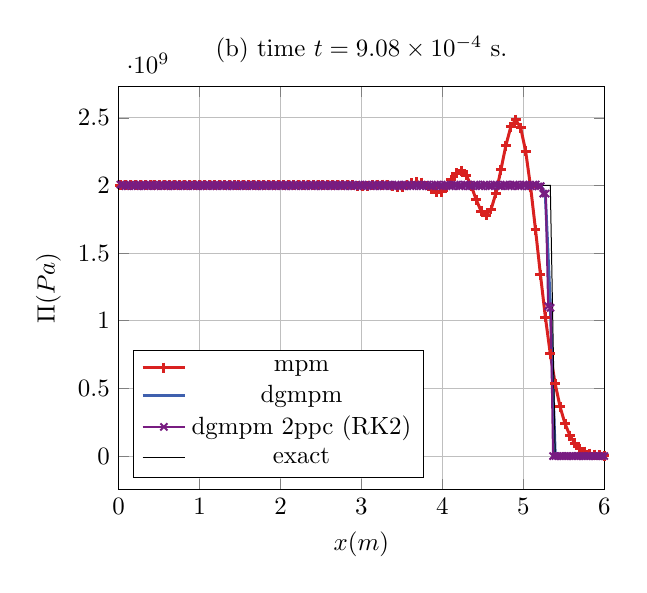
\begin{tikzpicture}[scale=0.9]
\begin{axis}[xlabel=$x (m)$,ylabel=$\Pi (Pa)$,ymajorgrids=true,xmajorgrids=true,legend pos= south west,title={(b) time $t = 9.08\times 10^{-4} $ s.},xmin=0.,xmax=6.]
\addplot[Red,very thick,mark=+,solid] coordinates {(-0.03923052052922343,2000240481.1233327) (0.021819761015892163,1999769738.8663158) (0.0828698927161351,2000218983.1347811) (0.1439199523557292,1999809950.54204) (0.20496998238621425,2000170838.6984289) (0.266019997207666,1999872129.80287) (0.32706999231126516,2000106436.8640933) (0.38811998365041567,1999944280.2454906) (0.449169959029736,2000038581.9512253) (0.510219934372632,2000013690.4345057) (0.5712698969291694,1999979089.5826085) (0.6323198600631447,2000070050.8467832) (0.6933698136476303,1999936253.3022394) (0.7544197669696648,2000107588.3199086) (0.8154697138768967,1999913395.649439) (0.876519659147888,2000125156.8768682) (0.9375696007168677,1999909211.6999958) (0.9986195394150338,2000126157.9927893) (1.059669476515721,1999919755.674749) (1.1207194099155477,2000115626.1187456) (1.1817693429480685,1999938103.4741611) (1.2428192719189772,2000098747.9520392) (1.3038692012782542,1999960657.9597352) (1.3649191269853391,2000083196.644746) (1.4259690532702223,1999982772.5176466) (1.4870189759372838,2000065998.3151865) (1.548068898510965,1999996968.6891499) (1.6091188183068375,2000054865.2647946) (1.670168739008601,2000018826.7281826) (1.731218658453022,2000056284.8743527) (1.7922685772512423,2000025238.8196642) (1.8533184921045645,2000031968.1138716) (1.9143684047609901,2000016400.7497857) (1.975418318053308,2000048568.7818315) (2.0364682364589175,2000073517.7988975) (2.097518157338219,2000081126.454338) (2.158568072062211,2000026752.5138342) (2.2196179727824346,1999962203.1821125) (2.2806678657928665,1999965067.139214) (2.341717771696925,2000088677.3296564) (2.4027677072086253,2000244140.0735695) (2.463817659277123,2000248079.915646) (2.5248675831316487,1999993716.8853536) (2.585917440063807,1999643305.288324) (2.646967250875889,1999579001.41102) (2.7080171068001158,2000062944.273291) (2.7690671011838006,2000852362.1540391) (2.830117219896753,2001206846.0073657) (2.8911672958158867,2000467231.4954524) (2.952217111542271,1998832793.1242473) (3.013266610958221,1997579685.768277) (3.0743160452078344,1998242489.666675) (3.1353658703158658,2001160849.0509126) (3.196416388566518,2004588933.5455565) (3.257467375954363,2005458038.2563794) (3.3185180466647264,2001697102.190524) (3.3795675234732467,1994541487.4730227) (3.440615585708569,1988762645.3894498) (3.5016631438647106,1989935602.9797668) (3.5627119421792885,2000111386.41128) (3.623763471464838,2014923977.0724418) (3.6848176974855837,2024790001.3711026) (3.7458725195458533,2020382377.2601633) (3.8069245712514714,1999447389.7073095) (3.8679711628702065,1970442647.6100123) (3.929012327573847,1949825797.016439) (3.9900516480144432,1953585186.3226125) (4.051095073761827,1987368815.1052973) (4.112148038363928,2040849436.9858987) (4.173212220481733,2090050737.5576959) (4.234283670427938,2107411656.1073942) (4.295353507700337,2075285788.362349) (4.356411206000879,1996293178.97995) (4.417449188621994,1894985293.978191) (4.478466731235185,1809589469.956608) (4.539471418899192,1777676873.8302789) (4.60047747902865,1822118201.7227845) (4.661501591798265,1942507354.7681544) (4.722557637422781,2114144751.4232287) (4.783652041946421,2294062789.964336) (4.844781069302256,2432159789.043516) (4.9059308043019065,2484574935.165112) (4.96707981812872,2425532064.97198) (5.028203724005535,2253708085.122853) (5.0892802390172465,1990804259.1885338) (5.150293249469595,1673238957.9983215) (5.211234847071616,1340859784.348242) (5.272105144435457,1027275994.3558226) (5.332910451399713,754633075.0224329) (5.393660750710443,533012801.80897325) (5.454367310619323,362876107.24577975) (5.515040918237955,238609504.42548501) (5.5756908552374504,151790024.9898157) (5.636324503231241,93541463.05793001) (5.696947375682255,55910425.71914032) (5.7575633798909625,32464567.359246336) (5.818175162719966,18385124.7089494) (5.878784450683184,10291867.039909834) (5.939392341636735,5971073.523642217) (5.999999537141593,4112438.7996382113) };
\addplot[Blue,very thick,mark=none,solid] coordinates {(-0.03942160478635286,2006060116.9510684) (0.021634703667567715,1993940137.594559) (0.08268599644388969,2006060373.9301388) (0.14373737764912256,1993939604.21122) (0.20478867280919388,2006061026.086628) (0.26584007847159263,1993938675.6310308) (0.32689134939619946,2006062073.480748) (0.38794277985880155,1993937351.85318) (0.4489940265576721,2006063516.189758) (0.5100454818139241,1993935632.8617878) (0.571096704298863,2006065354.3060572) (0.6321481843393669,1993933518.6248724) (0.6931993826243398,2006067587.9363937) (0.7542508874368217,1993931009.095019) (0.8153020615377354,2006070217.2044432) (0.876353591107017,1993928104.2093496) (0.9374047410418783,2006073242.2485344) (0.9984562953499471,1993924803.890371) (1.0595074211388207,2006076663.222377) (1.1205590001648187,1993921108.0437915) (1.1816101018298202,2006080480.2947278) (1.2426617055500626,1993917016.5617368) (1.3037127831153568,2006084693.6486328) (1.3647644115033453,1993912529.3202007) (1.4258154649951433,2006089303.4830647) (1.48686711802158,1993907646.1796832) (1.5479181474681376,2006094310.0113149) (1.6089698251009463,1993902366.9880114) (1.6700208305325863,2006099713.4611773) (1.7310725327370886,1993896691.5758796) (1.792123514186276,2006105514.0745523) (1.853175240924819,1993890619.7603688) (1.9142261984258384,2006111712.10775) (1.9752779496581556,1993884151.3441877) (2.0363288832474176,2006118307.831492) (2.097380658930556,1993877286.1154313) (2.1584315686465,2006125301.5292413) (2.21948336873485,1993870023.8487618) (2.28053425461794,2006132693.498629) (2.3415860790632617,1993862364.3047736) (2.4026369411559783,2006140484.0500283) (2.463688789907431,1993854307.2305677) (2.524739628254281,2006148673.5077674) (2.5857915012584574,1993845852.3584197) (2.6468423159059484,2006157262.2078867) (2.7078942131069095,1993836999.410417) (2.7689450041035615,2006166250.4990761) (2.8299969254428645,1993827748.093002) (2.891047692839202,2006175638.7426183) (2.9520996382559384,1993818098.1014004) (3.0131503821044743,2006185427.3114746) (3.074202351535314,1993808049.1178594) (3.13525307189056,2006195616.5906525) (3.196305065269774,1993797600.8137424) (3.2573557621882188,2006206206.9747465) (3.318407779447733,1993786752.8469522) (3.379458452987844,2006217198.8708515) (3.4405104940572713,1993775504.865476) (3.5015611442794836,2006228592.6960747) (3.562613209086164,1993763856.5055692) (3.6236638360528746,2006240388.8765044) (3.684715924521922,1993751807.3932695) (3.745766528297479,2006252587.8494554) (3.806818640351814,1993739357.1445801) (3.8678692210025045,2006265190.0607684) (3.9289213565629106,1993726505.364711) (3.9899719141569547,2006278195.9650536) (4.051024073142108,1993713251.6505055) (4.112074607749643,2006291606.0248404) (4.173126790076167,1993699595.5889838) (4.234177301769245,2006305420.7115803) (4.295229507351752,1993685536.758891) (4.356279996204306,2006319640.5037947) (4.4173322249554365,1993671074.7315753) (4.478382691043292,2006334265.886256) (4.539434942873767,1993656209.068866) (4.600485386274613,2006349297.3502934) (4.661537661093276,1993640939.3284109) (4.72258808188665,2006364735.3943052) (4.783640379600513,1993625265.0586715) (4.844690777867787,2006380580.5203645) (4.905743098382081,1993609185.8030493) (4.966793474206442,2006396833.2363412) (5.027845817424658,1993592701.0995812) (5.088896170891094,2006413494.1091921) (5.149948536715043,1993575783.3857787) (5.2109988679040695,2006188385.7824419) (5.272051199443885,1928173675.83211) (5.333086626305186,1114893331.7484362) (5.3939393939393945,0.0) (5.454545454545455,0.0) (5.515151515151516,0.0) (5.575757575757576,0.0) (5.636363636363637,0.0) (5.696969696969697,0.0) (5.757575757575758,0.0) (5.818181818181818,0.0) (5.878787878787879,0.0) (5.9393939393939394,0.0) (6.0,0.0) };
\addplot[Purple,thick,mark=x,solid] coordinates {(-0.03922301604942032,1994135003.8143709) (-0.009074837831142603,1994135327.5382233) (0.021523075320129238,2005865460.1935375) (0.051677994339231634,2005865540.6397502) (0.0822668758008341,1994135396.4583592) (0.11242345978014313,1994135442.2756677) (0.14301122575351569,2005866580.2736385) (0.17316819949872822,2005866583.7764273) (0.20375581897468137,1994135235.3830903) (0.23391286390200003,1994135281.970573) (0.26450034123994165,2005868078.4857993) (0.29465737837952566,2005868076.052185) (0.3252450076005887,1994134650.7495997) (0.3554020172291876,1994134716.185983) (0.38598951715446034,2005869987.9532342) (0.41614649494956335,2005869984.196581) (0.44673421042392686,1994133650.8641272) (0.4768911553029312,1994133736.3200936) (0.5074786957261858,2005872310.7698147) (0.5376356080195605,2005872305.9982176) (0.5682234130066373,1994132236.1149685) (0.5983802927916309,1994132341.6644566) (0.6289678733432371,2005875047.0253694) (0.6591247212380037,2005875041.269826) (0.6897126144378939,1994130406.364448) (0.7198694305893111,1994130532.0101562) (0.750457049772885,2005878196.6928372) (0.7806138348143057,2005878189.968179) (0.8112018146518958,1994128161.431707) (0.8413585687314308,1994128307.172391) (0.8719462249947207,2005881759.749104) (0.9021029487435118,2005881752.0713456) (0.93269101363723,1994125501.1181188) (0.9628477071998897,1994125666.9514115) (0.9934353990033135,2005885736.186498) (1.02359206300724,2005885727.5732303) (1.0541802113876557,1994122425.2141414) (1.0843368459731915,1994122611.1380703) (1.1149245717959766,2005890126.0066001) (1.145081177586202,2005890116.477569) (1.1756694078991365,1994118933.5003204) (1.20582598502954,1994119139.512731) (1.2364137433721918,2005894929.2238271) (1.2665702924608768,2005894918.8010514) (1.297158603170002,1994115025.7430112) (1.3273151243468142,1994115251.8416276) (1.3579029137342808,2005900145.8680048) (1.388059407611098,2005900134.575021) (1.418647797202381,1994110701.6970189) (1.4488042639020475,1994110947.8799276) (1.4793920829061942,2005905775.9789429) (1.5095485230651517,2005905763.8418655) (1.5401369901663489,1994105961.1079912) (1.5702934041634364,1994106227.373129) (1.6008812512548274,2005911819.6044917) (1.6310376400017392,2005911806.6511338) (1.6616261822127902,1994100803.712939) (1.691782545932699,1994101090.0580282) (1.7223704184836093,2005918276.7966) (1.7525267578346984,2005918263.0567758) (1.7831153730505365,1994095229.246782) (1.81327168818946,1994095535.669637) (1.84385958458336,2005925147.5690346) (1.8740158761491597,2005925133.0745907) (1.9046045627390318,1994089237.483962) (1.9347608308802464,1994089563.9823666) (1.9653487495801851,2005932431.753553) (1.9955049949309274,2005932416.5382469) (2.0260937512936668,1994082828.3726115) (2.0562499739975535,1994083174.944045) (2.0868379134903403,2005940128.4045188) (2.116994114177042,2005940112.50405) (2.1475829387283234,1994076002.632435) (2.1777391175363148,1994076369.2744386) (2.2083270763308156,2005948238.0659459) (2.2384832338849914,2005948221.518105) (2.269072125058446,1994068763.590026) (2.29922826149173,1994069150.2999275) (2.3298162381208245,2005956761.6554585) (2.359972354052955,2005956744.5004637) (2.3905613103018015,1994061110.0614216) (2.420717405859752,1994061516.8370643) (2.45130539888087,2005965699.5618157) (2.481461474678868,2005965681.8411288) (2.5120504944773168,1994053037.4510324) (2.5422065506359943,1994053464.2903204) (2.5727945586318346,2005975052.6724114) (2.6029505957595642,2005975034.4297986) (2.633539677604385,1994044544.567231) (2.663695695815098,1994044991.4683108) (2.694283717395741,2005984821.1414673) (2.7244397172916366,2005984802.422394) (2.755028859703366,1994035631.0282984) (2.7851848413913207,1994036097.989225) (2.8157728751957185,2005995004.9483852) (2.8459288392714592,2005994985.8002572) (2.8765180407956676,1994026296.6488297) (2.906673987358701,1994026783.6678703) (2.937262032055926,2006005604.0494888) (2.9674179616952228,2006005584.521593) (2.998007220903698,1994016541.2667468) (3.028163133711092,1994017048.3420172) (3.0587511880014775,2006016618.410417) (3.0889070845589246,2006016598.5542543) (3.119496400050816,1994006364.723129) (3.1496522804421927,1994006891.8527138) (3.180240343058371,2006028048.018772) (3.2103962078583868,2006028027.8874202) (3.240985578261241,1993995766.8365867) (3.271141427545555,1993996314.0189655) (3.3017294972534104,2006039892.8819644) (3.331885331589273,2006039872.530837) (3.3624747555599876,1993984747.4102676) (3.3926305750146017,1993985314.6443734) (3.42321865061413,2006052153.0306427) (3.453374455747092,2006052132.518732) (3.48396393197279,1993973306.2256682) (3.5141197228426364,1993973893.512831) (3.544707803168714,2006064828.5125036) (3.574863580327216,2006064807.9070828) (3.6054531075260225,1993961443.0478823) (3.635608871022857,1993962050.3986511) (3.666196954945923,2006077919.3870173) (3.6963527053248892,2006077898.7828076) (3.7269422822466223,1993949157.6075246) (3.7570980195483576,1993949785.0704486) (3.7876861059750215,2006091425.6997945) (3.8178418307352264,2006091405.2948232) (3.848431456162036,1993936449.554937) (3.878587168412147,1993937097.334268) (3.909175256285717,2006105347.3760405) (3.939330956553215,2006105327.7684526) (3.9699206293001703,1993923318.2738523) (4.000076317607094,1993923987.2069037) (4.030664405908172,2006119683.8346574) (4.060820082773636,2006119667.1966546) (4.0914098016895215,1993909762.099792) (4.121565467125785,1993910455.6078901) (4.15215355487327,2006134432.4522552) (4.182309209390719,2006134427.151202) (4.212898973359856,1993895775.1409583) (4.243054616959861,1993896507.1797674) (4.273642703213922,2006149582.4981947) (4.303798336396806,2006149621.3106256) (4.334388144345157,1993881334.3105564) (4.36454376709732,1993882161.7715528) (4.395131850970583,2006165091.373452) (4.4252874637767405,2006165303.257006) (4.455877314695601,1993866346.531625) (4.486032917511808,1993867501.231569) (4.516620998213603,2006180791.2370899) (4.546776591485469,2006181684.1461263) (4.57736648452554,1993850433.8838644) (4.607522068119923,1993852860.0486372) (4.638110145133578,2006196022.271079) (4.668265719357673,2006199597.6043155) (4.6988556542048805,1993832059.4747472) (4.72901121861128,1993839601.652889) (4.759599292405184,2006208192.2856772) (4.789754846743917,2006222336.4011028) (4.820344825122395,1993804972.4041867) (4.850500367772052,1993833278.5474827) (4.881088442652384,2006207119.6017978) (4.9112439710457245,2006262908.8673177) (4.941834002729241,1993743755.6062326) (4.97198951079214,1993856492.9333005) (5.002577606347889,2006152814.089386) (5.0327330818177884,2006372707.4450974) (5.063323208674937,1993545112.6047575) (5.09347862854396,1994001236.0147953) (5.124066825570078,2005887534.1138701) (5.15422213702806,2006754086.50732) (5.184812529057544,1992634221.3360858) (5.2149676447418924,1994471882.9187949) (5.245556232946693,1938971680.4954917) (5.275710927344704,1939500363.5698178) (5.306287365314434,1107312826.0054393) (5.336440679759463,1095683477.6733737) (5.366834170854271,0.0006575936376625943) (5.396984924623116,0.0006575936376625943) (5.427135678391959,0.0005380311580875769) (5.457286432160804,0.0004782499183000683) (5.487437185929648,0.0005380311580875769) (5.517587939698492,0.0004782499183000683) (5.547738693467337,0.0005380311580875769) (5.57788944723618,0.0004782499183000683) (5.608040201005025,0.00023912495915003393) (5.638190954773869,0.00023912495915003393) (5.668341708542713,0.0003586874387250511) (5.698492462311558,0.0003586874387250511) (5.7286432160804015,0.0005978123978750856) (5.758793969849246,0.0005978123978750856) (5.788944723618091,0.00023912495915003393) (5.819095477386934,0.00023912495915003393) (5.849246231155779,0.0003586874387250511) (5.879396984924623,0.0003586874387250511) (5.909547738693467,0.0004782499183000683) (5.939698492462312,0.0004782499183000683) (5.969849246231155,0.0) (6.0,0.0001793437193625254) };
\addplot[black,thin,mark=none,solid] coordinates {(-0.03942160478635286,2000000000.0000362) (0.021634703667567715,2000000000.0000362) (0.08268599644388969,2000000000.0000362) (0.14373737764912256,2000000000.0000362) (0.20478867280919388,2000000000.0000362) (0.26584007847159263,2000000000.0000362) (0.32689134939619946,2000000000.0000362) (0.38794277985880155,2000000000.0000362) (0.4489940265576721,2000000000.0000362) (0.5100454818139241,2000000000.0000362) (0.571096704298863,2000000000.0000362) (0.6321481843393669,2000000000.0000362) (0.6931993826243398,2000000000.0000362) (0.7542508874368217,2000000000.0000362) (0.8153020615377354,2000000000.0000362) (0.876353591107017,2000000000.0000362) (0.9374047410418783,2000000000.0000362) (0.9984562953499471,2000000000.0000362) (1.0595074211388207,2000000000.0000362) (1.1205590001648187,2000000000.0000362) (1.1816101018298202,2000000000.0000362) (1.2426617055500626,2000000000.0000362) (1.3037127831153568,2000000000.0000362) (1.3647644115033453,2000000000.0000362) (1.4258154649951433,2000000000.0000362) (1.48686711802158,2000000000.0000362) (1.5479181474681376,2000000000.0000362) (1.6089698251009463,2000000000.0000362) (1.6700208305325863,2000000000.0000362) (1.7310725327370886,2000000000.0000362) (1.792123514186276,2000000000.0000362) (1.853175240924819,2000000000.0000362) (1.9142261984258384,2000000000.0000362) (1.9752779496581556,2000000000.0000362) (2.0363288832474176,2000000000.0000362) (2.097380658930556,2000000000.0000362) (2.1584315686465,2000000000.0000362) (2.21948336873485,2000000000.0000362) (2.28053425461794,2000000000.0000362) (2.3415860790632617,2000000000.0000362) (2.4026369411559783,2000000000.0000362) (2.463688789907431,2000000000.0000362) (2.524739628254281,2000000000.0000362) (2.5857915012584574,2000000000.0000362) (2.6468423159059484,2000000000.0000362) (2.7078942131069095,2000000000.0000362) (2.7689450041035615,2000000000.0000362) (2.8299969254428645,2000000000.0000362) (2.891047692839202,2000000000.0000362) (2.9520996382559384,2000000000.0000362) (3.0131503821044743,2000000000.0000362) (3.074202351535314,2000000000.0000362) (3.13525307189056,2000000000.0000362) (3.196305065269774,2000000000.0000362) (3.2573557621882188,2000000000.0000362) (3.318407779447733,2000000000.0000362) (3.379458452987844,2000000000.0000362) (3.4405104940572713,2000000000.0000362) (3.5015611442794836,2000000000.0000362) (3.562613209086164,2000000000.0000362) (3.6236638360528746,2000000000.0000362) (3.684715924521922,2000000000.0000362) (3.745766528297479,2000000000.0000362) (3.806818640351814,2000000000.0000362) (3.8678692210025045,2000000000.0000362) (3.9289213565629106,2000000000.0000362) (3.9899719141569547,2000000000.0000362) (4.051024073142108,2000000000.0000362) (4.112074607749643,2000000000.0000362) (4.173126790076167,2000000000.0000362) (4.234177301769245,2000000000.0000362) (4.295229507351752,2000000000.0000362) (4.356279996204306,2000000000.0000362) (4.4173322249554365,2000000000.0000362) (4.478382691043292,2000000000.0000362) (4.539434942873767,2000000000.0000362) (4.600485386274613,2000000000.0000362) (4.661537661093276,2000000000.0000362) (4.72258808188665,2000000000.0000362) (4.783640379600513,2000000000.0000362) (4.844690777867787,2000000000.0000362) (4.905743098382081,2000000000.0000362) (4.966793474206442,2000000000.0000362) (5.027845817424658,2000000000.0000362) (5.088896170891094,2000000000.0000362) (5.149948536715043,2000000000.0000362) (5.2109988679040695,2000000000.0000362) (5.272051199443885,2000000000.0000362) (5.333086626305186,2000000000.0000362) (5.3939393939393945,0.0) (5.454545454545455,0.0) (5.515151515151516,0.0) (5.575757575757576,0.0) (5.636363636363637,0.0) (5.696969696969697,0.0) (5.757575757575758,0.0) (5.818181818181818,0.0) (5.878787878787879,0.0) (5.9393939393939394,0.0) (6.0,0.0) };
\legend{mpm,dgmpm,dgmpm 2ppc (RK2),exact}
\end{axis}
\end{tikzpicture}
%%% Local Variables:
%%% mode: latex
%%% TeX-master: "../../mainManuscript"
%%% End:
}
%   \caption{shock stress lower shock $5\sigma^y$}
%   \label{fig:he_low_shock}
% \end{figure}



%%% Local Variables:
%%% mode: latex
%%% TeX-master: "../mainManuscript"
%%% End:

\subsection{Plane strain problem}
\label{subsec:he_plate}
\subsubsection*{Two-dimensional plane strain problem}
% A two-dimensional rectangular plate made of the compressible hyperelastic neo-Hookean material is considered here in the plane strain case.
% Unlike for the Saint-Venant-Kirchhoff model, the polyconvexity of the neo-Hookean stored energy function ensures the hyperbolicity of the problem (see section \ref{sec:constitutive-equations}).
%Geometry, boundary and loading conditions are given in figure \ref{fig:2d_heDomain}.
% \begin{figure}[h!]
%   \centering
%   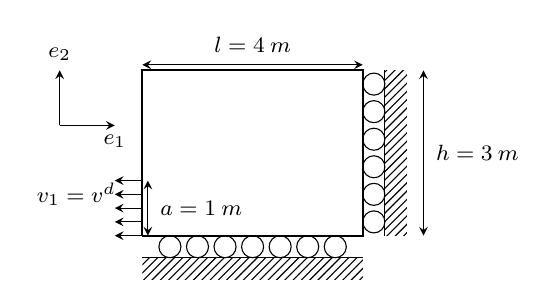
\begin{tikzpicture}[scale=0.7]
  \draw[thick] (0,0) --(4,0)--(4,3)--(0,3)--(0,0);
  \foreach \x in {0.5,1.,...,3.5} 
  \draw(\x,-0.2)circle(0.2);
  \foreach \x in {0.25,0.75,...,2.75} 
  \draw(4.2,\x)circle(0.2);
  \draw(0,-0.4)--(4.,-0.4);
  \draw(4.4,0)--(4.4,3);
  \fill [pattern=north east lines](0.0,-0.8)rectangle+(4,0.4);
  \fill [pattern=north east lines](4.4,0.)rectangle+(0.4,3);
  \draw[>=stealth,<->](5.1,0)--node[right=1pt]{\footnotesize $h=3 \: m$}(5.1,3);
  \draw[>=stealth,<->](0,3.1)--node[above=1pt]{\footnotesize $l=4 \: m$}(4,3.1);
  \draw[>=stealth,<->](0.1,0)--node[right=1pt]{\footnotesize $a=1 \: m$}(0.1,1);
  \foreach \x in {0.,0.25,...,1} 
  \draw[>=stealth,<-] (-0.5,\x)--(0.,\x);
  \node(a)at(-1.2,0.75){\footnotesize $v_1=v^d$}; 
  \draw[>=stealth,->](-1.5,2)--(-0.5,2)node(a)[anchor=north]{\footnotesize $\vect{e}_1$};
  \draw[>=stealth,->](-1.5,2)--(-1.5,3)node(a)[anchor=south]{\footnotesize $\vect{e}_2$};
\end{tikzpicture}

%%% Local Variables:
%%% mode: latex
%%% TeX-master: "../../mainManuscript"
%%% End:
%   \caption{Geometry, boundary and loading conditions of the two-dimensional problem in plane strain with a hyperelastic neo-Hookean material.}
%   \label{fig:2d_heDomain}
% \end{figure}
The plane strain problem studied in sections \ref{subsec:el_planestrain} and \ref{subsec:ep_planestrain} is now considered in a compressible hyperelastic neo-Hookean material submitted to a imposed velocity $v_1=-1000 \: m/s$ on the bottom part of its left end.
The solid is discretized such that material points are equivalent to $Q1$ finite element nodes, thus the plate is represented with $l \times h \equiv 28 \times 28$ material points, only with the 1ppc configuration.
The finite element computation is performed with the software \textit{Abaqus} \cite{Abaqus} using an explicit time discretization with no artificial viscosity added.
These numerical results are compared to those obtained from MPM and DGMPM using CTU computations.
The Courant number is set to unity in DGMPM and to $0.5$ in MPM leading to \textit{average} time steps $\Delta t_{CTU}=1.41 \times 10^{-5}s$ and $\Delta t_{MPM}=6.13 \times 10^{-6}s$, whereas the \textit{constant} time step used in the FEM simulation is $\Delta t_{FEM}=1.27 \times 10^{-5} s$.
Figure \ref{fig:2dhe_stress} shows numerical results in terms of the Cauchy stress tensor isovalues exported from Abaqus to the software Paraview \cite{Paraview} with the code developed in \cite{Export_Abaqus}, particularized to the present two-dimensional plane strain case.
Cauchy stress is plotted on the current configuration in such a way that figure \ref{fig:2dhe_stress} also enables the comparison on the deformed shape of the body.
\begin{figure}[h!]
  \centering
  \begin{tikzpicture}[scale=0.9]
  \begin{groupplot}[group style={group size=3 by 3,
      ylabels at=edge left, yticklabels at=edge left,
      horizontal sep=1.ex,
      vertical sep=2ex,},
    enlargelimits=0,
    xmin=0.,xmax=1., ymin=-0.,ymax=1.
    ,axis on top,scale only axis,xtick=\empty,ytick=\empty,width=0.25\linewidth,
    colorbar style={
      title style={
        font=\scriptsize,
        at={(1,.5)},
        anchor=north west
      },yticklabel style={font=\scriptsize}
      ,at={(current axis.south east)},anchor=south west
    }]
    %% FIRST ROW (time 1 = 2.3e-4s)
    %%% RANGE -6.5e9 -- 100e9
    \nextgroupplot[ylabel={$t=1.8\times 10^{-4} \:s$},title={(a) FEM}]\addplot graphics[xmin=0.,xmax=1., ymin=-0.,ymax=1.] {chapter4/pngFigures/he_fem_stress53.png};
    \nextgroupplot[title={(a) DGMPM}]\addplot graphics[xmin=0.,xmax=1., ymin=-0.,ymax=1.] {chapter4/pngFigures/he_dgmpm_stress53.png};
    \nextgroupplot[title={(c) MPM},
    colorbar,colorbar style={
      title= {$\sigma_{11}\: (GPa)$},
      ytick={-0.28,10},
      yticklabels={-2.8,100},
    }]
    \addplot[scatter,scatter src=y,mark size=0.pt] coordinates {(0.,-.28) (0.,10)};% Fake extreme values to fix scale
    \addplot graphics[xmin=-0.,xmax=1., ymin=-0.,ymax=1.] {chapter4/pngFigures/he_mpm_stress53.png};

    %% SECOND ROW (time 2 =6.5e-4s)
    %%% RANGE -7.1e9 -- 210e9
    \nextgroupplot[ylabel={$t=5.0\times 10^{-4} \:s$}]\addplot graphics[xmin=0.,xmax=1., ymin=-0.,ymax=1.] {chapter4/pngFigures/he_fem_stress176.png};
    \nextgroupplot[]\addplot graphics[xmin=0.,xmax=1., ymin=-0.,ymax=1.] {chapter4/pngFigures/he_dgmpm_stress176.png};
    \nextgroupplot[colorbar,colorbar style={
      title= {$\sigma_{11}\: (GPa)$},
      ytick={-0.42,19.},
      yticklabels={-4.2,190},
    }]
    \addplot[scatter,scatter src=y,mark size=0.pt] coordinates {(0.,-0.42) (0.,19)};% Fake extreme values to fix scale
    \addplot graphics[xmin=-0.,xmax=1., ymin=-0.,ymax=1.] {chapter4/pngFigures/he_mpm_stress176.png};

    %% THIRD ROW (time 2 =1.4e-3s)
    %%% RANGE -5.9e9 -- 330e9
    \nextgroupplot[ylabel={$t=1.0\times 10^{-3} \:s$}]\addplot graphics[xmin=0.,xmax=1., ymin=-0.,ymax=1.] {chapter4/pngFigures/he_fem_stress444.png};
    \nextgroupplot[]\addplot graphics[xmin=0.,xmax=1., ymin=-0.,ymax=1.] {chapter4/pngFigures/he_dgmpm_stress444.png};
    \nextgroupplot[colorbar,colorbar style={
      title= {$\sigma_{11}\: (GPa)$},
      ytick={-0.75,31.},
      yticklabels={-7.5,310},
    }]
    \addplot[scatter,scatter src=y,mark size=0.pt] coordinates {(0.,-0.75) (0.,31.)};% Fake extreme values to fix scale
    \addplot graphics[xmin=-0.,xmax=1., ymin=-0.,ymax=1.] {chapter4/pngFigures/he_mpm_stress444.png};
    
  \end{groupplot}
\end{tikzpicture}



%%% Local Variables:
%%% mode: latex
%%% TeX-master: "../mainManuscript"
%%% End:

  \caption{Isovalues of Cauchy stress tensor component $\sigma_{11}$ in a two-dimensional plate made of a neo-Hookean material, submitted to a velocity $\vect{v}\cdot\vect{e}_1=-1000 \: m/s$ on a part of its left end.}
  \label{fig:2dhe_stress}
\end{figure}
\begin{figure}[h!]
  \centering
  \input{chapter4/pgfFigures/linePlotshyp_stress}
  %\input{chapter4/pgfFigures/linePlotshyp_velo}
  \caption{Evolution of longitudinal Cauchy stress $\sigma_{11}$ along the bottom boundary of the domain.}
  \label{fig:he_lineplots_stress}
\end{figure}
At the beginning of the computation (first row in figure \ref{fig:2dhe_stress}), stress profiles are quite similar despite slight oscillations are visible in FEM and MPM solutions.
This can also be seen in figure \ref{fig:he_lineplots_stress}, in which stress is plotted along the bottom boundary of the domain.
However, MPM solution moreover exhibits, as for small strains problems, a concentration of stress in the high gradients region on the left boundary.
It is worth noticing that the DGMPM shows the same behavior that cannot be seen here due to the attenuation introduced by MPM stress values which are much higher.
The deformed shapes of the plate resulting from the three numerical approaches hence remain close, except at the junction of the loaded and free zones of the left edge.

When the pressure wave reflects on the fixed boundary at time $t=5.0\times 10^{-4}\:s$ (second row in figures \ref{fig:2dhe_stress} and \ref{fig:2dhe_velo}), the stress profiles are still similar though, FEM and MPM solutions oscillates even more.

These spurious oscillations are more significant in the velocity fields depicted in figures \ref{fig:2dhe_velo} as wall as in figure \ref{fig:he_lineplots_stress} and \ref{fig:he_lineplots_velo} which depicts the velocity the bottom boundary.
Furthermore, one can see in figure \ref{fig:he_lineplots_velo}\subref{subfig:he_velo2} that the homogeneous Dirichlet boundary condition is not exactly enforced in DGMPM when the incident wave hits the right end.
\begin{figure}[h!]
  \centering
  \begin{tikzpicture}[scale=0.9]
  \begin{groupplot}[group style={group size=3 by 3,
      ylabels at=edge left, yticklabels at=edge left,
      horizontal sep=1.ex,
      vertical sep=2ex,},
    enlargelimits=0,
    xmin=0.,xmax=1., ymin=-0.,ymax=1.
    ,axis on top,scale only axis,xtick=\empty,ytick=\empty,width=0.25\linewidth,
    colorbar style={
      title style={
        font=\scriptsize,
        at={(1,.5)},
        anchor=north west
      },yticklabel style={font=\scriptsize}
      ,at={(current axis.south east)},anchor=south west
    }]
    %% FIRST ROW (time 1 = 2.3e-4s)
    %%% RANGE -1.6e9 -- 7.8e10
    \nextgroupplot[ylabel={$t=1.8\times 10^{-4} \:s$},title={(a) FEM}]\addplot graphics[xmin=0.,xmax=1., ymin=-0.,ymax=1.] {chapter4/pngFigures/he_fem_velo53.png};
    \nextgroupplot[title={(a) DGMPM}]\addplot graphics[xmin=0.,xmax=1., ymin=-0.,ymax=1.] {chapter4/pngFigures/he_dgmpm_velo53.png};
    \nextgroupplot[title={(c) MPM},
    colorbar,colorbar style={
      title= {$v_1\: (m/s)$},
      ytick={-1.2,0.07},
      yticklabels={-1.2e3,70},
    }]
    \addplot[scatter,scatter src=y,mark size=0.pt] coordinates {(0.,-1.2) (0.,0.07)};% Fake extreme values to fix scale
    \addplot graphics[xmin=-0.,xmax=1., ymin=-0.,ymax=1.] {chapter4/pngFigures/he_mpm_velo53.png};

    %% SECOND ROW (time 2 =6.5e-4s)
    %%% RANGE -8.6e9 -- 1.3e11
    \nextgroupplot[ylabel={$t=5.0\times 10^{-4} \:s$}]\addplot graphics[xmin=0.,xmax=1., ymin=-0.,ymax=1.] {chapter4/pngFigures/he_fem_velo176.png};
    \nextgroupplot[]\addplot graphics[xmin=0.,xmax=1., ymin=-0.,ymax=1.] {chapter4/pngFigures/he_dgmpm_velo176.png};
    \nextgroupplot[colorbar,colorbar style={
      title= {$v_1\: (m/s)$},
      ytick={-1.1,0.11},
      yticklabels={-1.1e3,110},
    }]
    \addplot[scatter,scatter src=y,mark size=0.pt] coordinates {(0.,-1.1) (0.,0.11)};% Fake extreme values to fix scale
    \addplot graphics[xmin=-0.,xmax=1., ymin=-0.,ymax=1.] {chapter4/pngFigures/he_mpm_velo176.png};

    %% THIRD ROW (time 2 =1.4e-3s)
    %%% RANGE -2.8e8 -- 1.8e11
    \nextgroupplot[ylabel={$t=1.0\times 10^{-3} \:s$}]\addplot graphics[xmin=0.,xmax=1., ymin=-0.,ymax=1.] {chapter4/pngFigures/he_fem_velo444.png};
    \nextgroupplot[]\addplot graphics[xmin=0.,xmax=1., ymin=-0.,ymax=1.] {chapter4/pngFigures/he_dgmpm_velo444.png};
    \nextgroupplot[colorbar,colorbar style={
      title= {$v_1\: (m/s)$},
      ytick={-1.,0.12},
      yticklabels={-1e3,120},
    }]
    \addplot[scatter,scatter src=y,mark size=0.pt] coordinates {(0.,-1.1) (0.,0.12)};% Fake extreme values to fix scale
    \addplot graphics[xmin=-0.,xmax=1., ymin=-0.,ymax=1.] {chapter4/pngFigures/he_mpm_velo444.png};
    
  \end{groupplot}
\end{tikzpicture}



%%% Local Variables:
%%% mode: latex
%%% TeX-master: "../mainManuscript"
%%% End:

  \caption{Isovalues of velocity component $v_1$ in a two-dimensional plate made of a neo-Hookean material, submitted to a velocity $\vect{v}\cdot\vect{e}_1=-1000 \: m/s$ on a part of its left end.}
  \label{fig:2dhe_velo}
\end{figure}
\begin{figure}[h!]
  \centering
  {\phantomsubcaption \label{subfig:he_velo1}}
  {\phantomsubcaption \label{subfig:he_velo2}}
  {\phantomsubcaption \label{subfig:he_velo3}}
  \input{chapter4/pgfFigures/linePlotshyp_velo}
  \caption{Evolution of horizontal velocity $v_1$ along the bottom boundary of the domain.}
  \label{fig:he_lineplots_velo}
\end{figure}
This can be explained by considering a boundary cell of the arbitrary grid (\textit{i.e. containing one material point that belong to the right end of the domain}) that is about to be reached by the wave through the upwind interface.
The intercell flux on the upwind interface resulting from the discontinuity, and subsequently the conserved quantities vector resulting from the solution of the discrete system on the grid, are non-zero.
In particular, the horizontal velocity at upwind nodes of the boundary cell does not vanish while that of the downwind edge satisfies the homogeneous Dirichlet condition. 
Hence, the interpolation of the velocity from nodes to the particle yield a non-zero field at the material point level.
Note that it holds for the MPM as well in which the enforcement of boundary conditions is still a challenging question \cite{BC_MPM}.

Nevertheless, no significant displacements of particles can be seen on the right end in MPM and DGMPM solutions in figures \ref{fig:2dhe_stress} and \ref{fig:2dhe_velo}.
At last, oscillations remain in FEM and MPM solutions until the end of the simulation. 
Since the velocity field depicted in figures \ref{fig:2dhe_velo} and \ref{fig:he_lineplots_velo} is used to update the shape of the solid in FEM, the numerical noise yields final configurations that are slightly different.
On the other hand, updating particles position with the grid velocity within the MPM allows to get better results than if the oscillating material points velocity was used.


%%% Local Variables:
%%% mode: latex
%%% TeX-master: "../mainManuscript"
%%% End:



\section{Conclusion}
%%% Local Variables:
%%% mode: latex
%%% TeX-master: "../mainManuscript"
%%% End:


%% Chapter 5: Numerical Results
%\chapter{Contribution to the solution of elastic-plastic problems in two space dimensions}
%% Faire un historique des formulations faites.
%% Formuler le problème à notre sauce et identifier les cas évoqués en intro en particularisant les modules tangents etc. a ce moment, parler des trajets de chargement et des types d'ondes

\section*{Introduction}
It has been shown throughout this manuscript that hyperbolic problems in solid mechanics are solved in a different manner depending on the numerical explicit method employed. 
In particular, irreversible deformations which are usually numerically computed based on well-known constitutive integrators, may greatly differ from one scheme to another even for one-dimensional problems.
However, the accurate assessment of residual stresses and strains are of major importance for many industrial applications such as, among others, high-speed metal forming, crash-proof design or the study of the impact of earthquakes on structures.
The simulations performed in chapter \ref{chap:chap4} emphasized the improvements enabled by the knowledge of the characteristic structure of the solutions of conservation laws systems, especially for elastoplastic solids.
Nevertheless, the introduction of the exact solution by means of approximate Riemann solvers is so far only possible for problems in one space dimension in elastic-plastic solids.

The purpose of this chapter is to identify typical behaviors of the solutions of two-dimensional elastoplasticity problems under small strains.
%The purpose of this chapter is to provide solutions and clues for future works for general two-dimensional elastoplasticity problems under small strains. 
The knowledge one can get about these solutions allows a better understanding of the physical phenomena occuring and hence, the ability to accurately deal with them numerically.
% More information on the structure of solutions to these problems allow a better understanding of physical phenomena occuring in media on the one hand, and the ability of accurately deal with them numerically on the other hand.

The chapter is organized as follows.
A brief historical review of the solution of dynamic problems in two-dimensional elastic-plastic solids is made in section \ref{sec:review}.
%A brief historical review of the solution of plastic waves in two-dimension space is made in section \ref{sec:review}.
Then, the equations of plasticity are recalled in section \ref{sec:charac_plast} so that the characteristic analysis, followed by the application of the method of characteristics, can be carried out.
In section \ref{sec:stress_paths}, attention is paid to the evolution of stress components inside the simple waves that might propagate by means of a mathematical study of the ODEs satisfied within the simple waves.
Since the developments rapidly become cumbersome, the analysis is supplemented with numerical results in section \ref{sec:stress_paths_num}.
%Attention is next paid in section \ref{sec:stress_paths} to the evolution of stress components through simple waves possibly arising in the solution. 
At last, some identified trends are discussed at the end of the chapter in order to use them for the building of a dedicated Riemann solver. 

\section{Historical review}
\label{sec:review}
% Researches done on the elastic-plastic bahavior of material at high strain rates for characterization purposes. 
% To this end, uni-axial stress or strain, pure bending or pure torsion problems have been investigated until the late 50's (vérifier ça). 
% Rakmathulin et Cristescu ont ouvert la voie à des problèmes plus complexes impliquant des chargements combinés.

% Elastic solver used previously

% \cite{Clifton_thesis} development of a method of characteristics in 3 independent variables that is then numerically approximated (Notion of bicharacteristics). Nous on n'en a pas besoin puisqu'on a déjà notre schéma numérique. En ravanche, on cherche à résoudre le problème dans une direction donnée pour lequel la méthode des caractéristiques s'applique.

% This is for instance the case for the simulation of forming technics that cannot, in general, be modeled in a one-dimensional setting.

Until the 50s, researches on dynamic problems in plastic solids were focused on uni-axial stress or strain, pure bending or pure torsion loading conditions \cite{Taylor,vonKarman}, and were carried out for materials characterization purposes.
The first references that brought some understanding about the response of linearly hardening solids to combined shear and pressure loads are those of Rakhmatulin \cite{Rakhmatulin} and Cristescu \cite{CRISTESCU19591605}.
These early analytical investigations on plane stress impacts in the plastic regime led to the conclusion that elastic waves, as well as plastic combined-stress simple waves, can propagate in two-dimensional solids. 
While the former were well-known, the latter were shown to fall into the two \textit{fast waves} and \textit{slow waves} families.
The maximal value of fast waves (\textit{resp. slow waves}) is higher than that of pressure (\textit{resp. shear}) plastic discontinuity occuring in one-dimensional problems, for a given compression (\textit{resp. shear}) load amplitude.

Later, Bleich and Nelson \cite{Bleich} considered sumperimposed plane and shear waves in an ideally elastic-plastic materials submitted to step loads.
It has thus been highlighted that different loading cases yield different characteristic structures of the solution of a Picard problem, thus revealing the complexity of plastic flows in more than one dimension.
% Distinguer un peu plus ces deux contributions.
%\thomas{see \cite[p.56 pdf]{Nowacki},\cite{Goel}}. 
The same conclusions have been drawn by Clifton \cite{Clifton} for hardening materials under tension-torsion, who furthermore studied the influence of plastic pre-loading on the solution.
This contribution established the existence of loading paths through the simple waves arising from the characteristic analysis of the hyperbolic system.
Indeed, the combined-stress wave nature lies in ODEs which govern the evolution of stress components within the simple waves.
The integration of these equations of the form $d\sigma_{11}=\psi d\sigma_{12}$ allows the building of curves which connect the applied stress state of the Picard problem $(\sigma^d_{11},\sigma^d_{12})$ to the initial state of the medium.
% Indeed, the study mathematical properties of relations between stress components of the form $d\sigma_{11}=\psi d\sigma_{12}$, satisifed inside fast and slow simple waves, allows to connect the applied stress state of the Picard problem $(\sigma^d_{11},\sigma^d_{12})$ to the initial state of the medium.
It has been for instance shown that if a solid is acted upon by a traction force such that $\sigma^d_{11}=0$ and $\sigma^d_{12}$ lies outside the elastic convex, only an elastic shear discontinuity, followed by a slow simple wave, propagates.
Conversely, other loading conditions may lead to the combination of elastic pressure discontinuity and a fast wave, possibly followed by a slow wave.
Another notable conclusion is that the combined loading paths followed inside simple waves may lead to plastic unloading, while only elastic unloading occurs in the one-dimensional theory.
%In addition, it is possible to meet unloading plastic simple waves with contrast to the one-dimensional theory in which the unloading waves propagate at elastic speeds (c'est pas vraiment ça attention).
%Such loading paths are supplemented by ODEs satisfied by the velocity components so that a closed form of the solution of the problem can be derived.

Experimental data collected on a thin-walled tube submitted to a dynamic tensile load \cite{Clifton_exp,Clifton_exp2} confirmed the existence of two distinct families of  simple waves, both involving combined stress paths.
Those works nevertheless exhibited some discrepancies with the theory which have been attributed to the assumption made on the von-Mises yield surface.
As a matter of fact, a constant strain region lying between the fast and slow waves that is predicted by the theory \cite{Clifton} could not be seen in experimental results.
However, by following the endochronic theory of plasticity \cite{Valanis} which does not require the introduction of a yield surface, Wu and Lin \cite{Wu_experimental} obtained numerical results that better fitted the experimental data provided by Lipkin and Clifton \cite{Clifton_exp2}.
The good agreement showed between numerical and experimental results \cite{Wu_experimental} thus confirmed the theory.

Ting and Nan \cite{Ting68} then generalized the work of Bleich and Nelson to hardening materials and Ting \cite{Ting69} widened this of Clifton to more complex loadings, that is a superimposition of one plane wave and two shear waves states.
Once again, the mathematical study of the ODE system governing the stresses evolution inside fast and slow simple waves led to the construction of loading paths in the stress space that depend on the external loads. A review of governing equations for all the cases depending on one space dimension considered above can be found in \cite{Nowacki}.

The information on characteristic structures thus provided has then be used by Lin and Ballman \cite{Lin_et_Ballman} for the development of an iterative Riemann solver.
This procedure is based on successive guesses on the stress state lying in the stationary region so that the loading paths preticted by the theory of Clifton \cite{Clifton} can integrated numerically until convergence.
The implementation of this solver within a second-order Godunov scheme provided results that were in good agreement the exact solutions.
Nevertheless, the theoretical investigations mentioned above restrict the development of such numerical tools to problems that depend on one space dimension.
%%
Clifton tackled the solution of plane strain problems in elastic-plastic solids by looking for bi-characteristics \cite{Clifton_thesis} in order to build finite difference schemes that account for plastic waves.
The point of view adopted here is that one can benefit from the simplifications introduced by the writing of Riemann problems in an arbitray direction of space.
Indeed, the method of characteristics rather than the more complex method of bi-characteristics can be employed with the quasilinear forms presented in chapter \ref{chap:chap2}.




%%% Local Variables:
%%% mode: latex
%%% TeX-master: "../mainManuscript"
%%% End:


\section{Elastic-plastic wave structure in two space dimensions}
\label{sec:charac_plast}
We assume the infinitesimal strain tensor can be additively decomposed into an elastic part and a plastic part according to:
\begin{equation}
  \label{eq:ch5_partition}
  \tens{\eps}=\tens{\eps}^e+\tens{\eps}^p
\end{equation}
The elastic part of the infinitesimal strain tensor is:
\begin{equation}
  \label{eq:ch5_elastic_inverse}
  \tens{\eps}^e = \frac{1+\nu}{E} \tens{\sigma} - \frac{\nu}{E} \tr \tens{\sigma} \tens{I}
\end{equation}

\subsubsection*{The general case}
The governing equations of dynamics in elastic-plastic solids are written in the following quasi-linear form:
\begin{equation}
  \Qcb_t + \Absf^i \drond{\Qcb}{x_i} = \Scb \qquad \text{with: }\Absf^i = -\matrice{\tens{0}^2 & \frac{1}{\rho}\tens{I}\otimes\vect{e}_i\\ \Cbb^{ep}\cdot \vect{e}_i & \tens{0}^4}  \label{eq:ch5_quasilinear}
\end{equation}
where $\Qcb=\matrice{\vect{v}\\ \tens{\sigma}}$ and $\Cbb^{ep}=\ddroit{\tens{\sigma}}{\tens{\eps}}=\Cbb - \beta\tens{m}\otimes\tens{m}$ is the tangent modulus with $\tens{m}=\frac{\tens{s}-\tens{Y}}{\norm{\tens{s}-\tens{Y}}}$ is the flow direction and $\beta=\frac{6\mu^2}{3\mu +(C+R')}$ depends on the shear modulus $\mu$ and kinematic or isotropic hardening modulus $C$ and $R'$ (see section \ref{sec:constitutive-equations}). In particular in the arbitrary direction $\vect{n}$:
\begin{equation}
  \Qcb_t + \Jbsf \drond{\Qcb}{x_n} = \Scb  \label{eq:ch5_quasilinear_normal}
\end{equation}
where $x_n=\vect{x}\cdot\vect{n}$ and the Jacobian matrix $\Jbsf=\Absf^in_i$ arises. The left characteristic fields $\{c_K;\Lcb^K\}$ satisfy the following equation:
\begin{equation}
  \label{eq:ch5_eigen_system}
  \vect{\Lc}^K \(\Jbsf - c_K \Ibsf\) = \vect{0}
\end{equation}
As seen in section \ref{sec:characteristic_analysis}, $6$ couples of characteristic speeds $c_K$ and left eigenvectors $\Lcb^K= \[ \vect{v}^K \: , \: \tens{S}^K \]$ are determined based on those of the acoustic tensor $\tens{A}=\vect{n}\cdot\Cbb^{ep}\cdot \vect{n}$, that are $\{\omega^p;\vect{l}^p\}$ for $p=1,2,3$:
\begin{equation}
  \label{eq:ch5_left_eigenfields}
  \left\lbrace \pm \sqrt{\frac{\omega_p}{\rho_0}} ; \quad \[\: \pm \rho_0\sqrt{\frac{\omega_p}{\rho_0}} \vect{l}^p , -\vect{l}^p\otimes \vect{N} \:\]  \right\rbrace ,\quad p=1,2,3
\end{equation}
In addition, three independent left eigenvectors associated to the zero eigenvalue of system \eqref{eq:ch5_quasilinear_normal}, which is of multiplicity $3$, are found by solving:
\begin{equation}
  \label{eq:ch5_null_eigen}
  \tens{\sigma}^K:\(\Cbb^{ep}\cdot  \vect{n}\) =\vect{0},\quad K=1,2,3
\end{equation}

\subsubsection*{Problems in two space dimensions}
We now focus on the solid domain bounded by $x_1 \times x_2 \times x_3 \in [0,\infty[ \times ]-infty,infty[ \times [-e,e]$ in a Cartesian coordinates system, where $e$ is an arbitrary length.
The solid is subject on the plane $x_1=0$ to a traction force $\vect{T}$ restricted to the $(\vect{e}_1,\vect{e}_2)$ plane, that is $T_3=0$. It is moreover assumed that all quantities except the velocity component $v_3$ depend solely on $x_1$ and $x_2$.

First, the solid is under plane strain, that is $\tens{\eps}\cdot\vect{e}_3=\vect{0}$, if the velocity $v_3$ vanishes on both ends $x_3=\pm h$. Thus, combination of equations \eqref{eq:ch5_partition} and \eqref{eq:ch5_elastic_inverse}, along with the kinematic condition $\eps_{33}=0$, allows to write a relation between $\sigma_{33}$ and other stress components:
\begin{equation}
  \label{eq:plane_strain_stress33}
  \sigma_{33}=\nu\(\sigma_{11}+\sigma_{22}\) - E\eps^p_{33}
\end{equation}

Conversely, if the planes $x_3=\pm e$ are traction free, a plane stress state reading $\tens{\sigma}\cdot\vect{e}_3=\vect{0}$ holds in the solid. For both plane strain and plane stress problems, the stress component $\sigma_{33}$ can then be removed from system \eqref{eq:ch5_quasilinear_normal}, leading to the unknown vector $\Qcb=[v_1,v_2,\sigma_{11},\sigma_{22},\sigma_{12}]$. The problem can then be solved in a two-dimensional setting, for which the acoustic tensor admits two distinct real eigenvalues:
\begin{subequations}
  \begin{alignat}{1}
    \label{eq:ch5_eigenAcc1}
    &\omega_1 = \frac{1}{2}\(A_{11}+A_{22} - \sqrt{(A_{11}-A_{22})^2+4A_{12}}\) \\
    \label{eq:ch5_eigenAcc2}
    &\omega_2 = \frac{1}{2}\(A_{11}+A_{22} + \sqrt{(A_{11}-A_{22})^2+4A_{12}}\) 
  \end{alignat}
\end{subequations}
with associated left eigenvector:
\begin{equation}
  \label{eq:ch5_eigenvectAcc}
  \vect{l}^p=\matrice{-A_{12} \\ A_{11}-\omega_p} = \matrice{ A_{22}-\omega_p \\ -A_{12}}
\end{equation}
From equation \eqref{eq:ch5_left_eigenfields}, one gets that the problem involves two families of waves travelling at speeds $c_1 = \pm \sqrt{\omega_1/\rho}$ and $c_2 = \pm \sqrt{\omega_2/\rho}$. For elastic evolutions, th

that are referred to as \textit{slow} and \textit{fast} waves, travelling respectively at speeds $c_s = \pm \sqrt{\omega_1/\rho}$ and $c_f = \pm \sqrt{\omega_2/\rho}$.
Considering equation \eqref{eq:ch5_left_eigenfields}, the problems involve 









% Orthogonalité des loading paths \cite{Clifton,Ting68}

%%% Local Variables:
%%% mode: latex
%%% TeX-master: "../mainManuscript"
%%% End:


\section{Loading paths through simple waves}
\label{sec:stress_paths}
% On ne regarde qu'une dimension spatiale en faisant des hypothèse sur les champs alors que nous on se limite à une direction particulière $\vect{n}$.
% En plus, on se limite à l'étude d'ondes simples alors que des chocs peuvent exister (voir Mandell car il semble y etre démontré que les shock n'arrivent que pour $\tau=0$).
% Il y a la question des vitesses charactéristiques plastiques... sont-elles collées aux vitesses élastiques ?
% dependance des vitesses caractéristiques à l'angle entre la direction principale de sigma et la direction de propagation, c'est dit dans la thèse de Clifou en page 90.

\subsection{Properties of the loading paths}
The stress paths followed within slow and fast simple waves is governed by the mathematical properties of functions $\psi^s_1$ and $\psi^f_1$ involved in the relations of table \ref{tab:simpleWavesEquations}.
Then, before specializing the discussion to plane stress and plane strain cases, some general properties holding regardless of the loading conditions are highlighted.
The analysis is here carried out for the special case $\vect{n}=\vect{e}_1$, similar results being obtained for the other situation $\vect{n}=\vect{e}_2$.

First, the functions are orthogonal in the stress space, that is $\psi^s_1\psi^f_1=-1$.
Indeed, considering the left eigenvectors of the acoustic tensor in equation \eqref{eq:ch5_eigenvectAcc}, the product $\psi^s_1\psi^f_1$ reads:
\begin{equation*}
  \psi^s_1\psi^f_1 = \frac{l^1_2}{l^1_1}\: \frac{l_2^2}{l^2_1} = \frac{(A_{11}-\omega_2)A_{12}}{(A_{22}-\omega_1)A_{12}}
\end{equation*}
Introduction of the expressions of eigenvalues $\omega_i$ from equations \eqref{eq:ch5_eigenAcc1} and \eqref{eq:ch5_eigenAcc1} further yields:
\begin{equation*}
  \psi^s_1\psi^f_1 = \frac{A_{11} -A_{22} +\sqrt{(A_{11} -A_{22} )^2 + 4A_{12}^2 }}{A_{22} -A_{11} -\sqrt{(A_{11} -A_{22} )^2 + 4A_{12}^2 }}=-1
\end{equation*}
In other words, $\vect{l}^1 \cdot \vect{l}^2=0$ as expected by the symmetry of $\tens{A}$.
This orthogonality has already been noticed for particular plane strain and plane stress cases \cite{Clifton,Ting68} but now obviously appears as true for all problems in two space dimensions.
%Moreover, since $\psi^s_2=1/\psi^s_1$ and $\psi^f_2=1/\psi^f_1$, the same holds for the functions $\psi^s_2$ and $\psi^f_2$.
Therefore, it allows us to restrict the study to one function only, say $\psi_1^f$.

Second, if the function $\psi_1^f$ vanishes at some point of the stress space, the projection of the stress path in the $(\sigma_{11},\sigma_{12})$ plane is vertical according to the ODE \eqref{eq:sigSlow_n=e1}.
Conversely, if the inverse of $\psi_1^f\rightarrow \infty$, the loading path is horizontal in the $(\sigma_{11},\sigma_{12})$ plane.
%Looking for vanishing $\psi^f_1$ or $1/\psi^f_1$ amounts to finding roots of the components of $\vect{l}^2$:
It then comes out:
\begin{subequations}
  \begin{alignat}{1}
    \label{eq:first_root}
    \psi_1^f = 0  & \Leftrightarrow A_{12} =0  \\
    \label{eq:second_root}
    \psi_1^f\rightarrow \infty & \Leftrightarrow A_{11} -\omega_2 =0
  \end{alignat}
\end{subequations}
In particular, if $A_{12}=0$ the second equation reads:
\begin{equation}
  A_{11} -\omega_2 = \frac{1}{2}\(A_{11} -A_{22} +\sqrt{(A_{11} -A_{22} )^2 + 4A_{12}^2 }\) = \left\langle A _{11}-A _{22}  \right\rangle
\end{equation}
where $\left\langle \bullet \right\rangle$ denotes the positive part operator.
Hence, if $A_{12} =0$ and $A_{11} \neq A_{22} $, one has $\psi^f_1 \rightarrow \infty$ and $\psi^s_1 = 0$, so that the stress path in the ($\sigma_{11},\sigma_{12}$) plane are horizontal (\textit{resp. vertical}) through a fast (\textit{resp. slow}) wave. 
On the other hand, if $A_{11}  = A_{22} $, both components of the eigenvectors vanish and the functions $\psi^f_1$ and $\psi^s_1$ are undetermined.
At last, it follows from equation \eqref{eq:diff_celerities} that the simultaneous of conditions \eqref{eq:first_root} and \eqref{eq:second_root} leads to characteristic speeds of simple waves that are identical. Hence, the situation $c_f=c_s$ corresponds to a loss of hyperbolicity of the system.


The above discussion is now specified to plane stress and plane strain, for which loading conditions leading to $A_{12} =0$ and $A _{11}-A _{22}=0$ are identified.
\subsection{The plane stress case}
The case of plane stress is first considered by using the tengent modulus of equation \eqref{eq:CP_constitutive}.
\begin{subequations}
  \begin{alignat}{1}
    \label{eq:CP_A11}
    & \tilde{A}_{11}^{ep}= \tilde{C}^{ep}_{1111} - \frac{(\tilde{C}^{ep}_{1133})^2}{\tilde{C}^{ep}_{3333}} = \lambda + 2\mu -\beta s_{11}^2 -\frac{\(\lambda -\beta s_{11}s_{33}\)^2}{\lambda + 2\mu - \beta s_{33}^2} \\
    \label{eq:CP_A22}
    & \tilde{A}_{22}^{ep}= \tilde{C}^{ep}_{1212} - \frac{(\tilde{C}^{ep}_{1233})^2}{\tilde{C}^{ep}_{3333}}= \mu - \beta s_{12}^2 -\frac{\(\beta s_{12}s_{33}\)^2}{\lambda + 2\mu - \beta s_{33}^2} \\
    \label{eq:CP_A12}
    & \tilde{A}_{12}^{ep} = \tilde{C}^{ep}_{1112} - \frac{\tilde{C}^{ep}_{1133}\tilde{C}^{ep}_{1233}}{\tilde{C}^{ep}_{3333}} =\beta s_{12} \frac{\lambda s_{33} - (\lambda + 2\mu)s_{11} }{\lambda + 2\mu - \beta s_{33}^2} 
  \end{alignat}
\end{subequations}

First, in order to ensure the hyperbolicity of the system, the component of the acoustic tensor also have to be defined, that is $\tilde{C}^{ep}_{3333}\neq 0$. This condition leads to:
\begin{equation*}
  \lambda + 2\mu - \beta s_{33}^2 \neq 0 \quad \Leftrightarrow \quad s_{33}\neq \frac{\lambda + 2\mu}{\beta}
\end{equation*}

Second, from equation \eqref{eq:CP_A12}, $\tilde{A}_{12}^{ep}$ admits two roots in terms of the components of the deviatoric stress tensor, namely: 
\begin{equation}
  s_{12}=0 \quad ; \quad s_{11}= \frac{\lambda}{\lambda+2\mu}s_{33}
\end{equation}
In terms of the components of Cauchy stress tensor, those conditions read:
% \begin{align}
%   & \frac{2}{3}\sigma_{11}-\frac{1}{3}\sigma_{22} = -\frac{\lambda}{3\lambda+6\mu}(\sigma_{11}+\sigma_{22}) \\
%   & 2\sigma_{11}-\sigma_{22} = -\frac{\lambda}{\lambda+2\mu}(\sigma_{11}+\sigma_{22}) \\
%   & \sigma_{11}(2 +\frac{\lambda}{\lambda+2\mu})=\sigma_{22}(1-\frac{\lambda}{\lambda+2\mu})\\
%   & \sigma_{11}\frac{3\lambda+4\mu}{\lambda+2\mu}=\sigma_{22}\frac{2\mu}{\lambda+2\mu}\\
%   & \sigma_{11}=\sigma_{22}\frac{2\mu}{3\lambda+4\mu}
% \end{align}
\begin{equation}
  \label{eq:CP_roots}
  \sigma_{12}=0 \quad ; \quad \sigma_{11}=\frac{2\mu}{3\lambda+4\mu}\sigma_{22}
  % \sigma_{12}=0 \quad ; \quad \sigma_{11}=\frac{1-2\nu}{2-\nu} \sigma_{22}
\end{equation}
Hence, the loading path through a fast simple wave is vertical, that is $\psi^f_1 = 0$, for stress values satisfying \eqref{eq:CP_roots}, providing that the $\tilde{A}_{11}^{ep}$ and $\tilde{A}_{22}^{ep}$ are not equal.
Conversely, such stress states yield horizontal path through a slow wave.
\begin{remark}
  \label{rq:loading_paths_CP1}
  The latter result is particularly interesting if considering a loading path starting from a point of the plane $\sigma_{12}=0$.
  Indeed, the loading path followed through a slow simple wave (equation \eqref{eq:sigSlow_n=e1}) is such that $d\sigma_{12}=0$ so that no change in that component of stress occurs.
\end{remark}
%% Attempt to show that if s12=0, cs=c2 but depends on the sign of A11-A22
% \begin{align}
%   &\omega_2=\frac{1}{2}\(A_{11}+A_{22} - \abs{A_{11}-A_{22}}\)\\
%   &\omega_2=\frac{1}{2}\(A_{11}+A_{22} - A_{11}+A_{22}\) \quad ;\quad \omega_2=\frac{1}{2}\(A_{11}+A_{22} + A_{11}-A_{22}\) \\
%   &\omega_2=A_{22} \quad ;\quad \omega_2=A_{11}
% \end{align}


% \paragraph*{Case $s_{12}=0$ :}
% \begin{align}
%   & \rho c_s^2 =\frac{1}{2}\(\tilde{A}_{11}^{ep}+\tilde{A}_{22}^{ep} - \abs{\tilde{A}_{11}^{ep}-\tilde{A}_{22}^{ep}}\) \\
%   & \rho c_f^2 =\frac{1}{2}\(\tilde{A}_{11}^{ep}+\tilde{A}_{22}^{ep} + \abs{\tilde{A}_{11}^{ep}-\tilde{A}_{22}^{ep}}\)
% \end{align}

If on the other hand, on considers the vector $\vect{n}=\vect{e}_2$, the same procedure as above yields:

????????????????????????????????????????????????????????

\textit{Brief summary of the results.}


The complexity introduced by the plane stress tangent modulus prevent the finding of other singular configurations for the hyperbolic system. 
In particular, it is difficult to deal with the equation $\tilde{A}^{ep}_{11}=\tilde{A}^{ep}_{22}$ with the expressions given in equations \eqref{eq:CP_A11} and \eqref{eq:CP_A22}.
As we shall see below, more singular behavior can be identified for plane strain.




\subsection{The plane strain case}
% The expressions of the tangent modulus and the acoustic tensors are recalled here for convenience:
% \begin{align}
%   & C^{ep}_{ijkl} = \lambda \delta_{ij}\delta_{kl} + \mu \(\delta_{il}\delta_{jk} + \delta_{ik}\delta_{jl}\) - \beta s_{ij}s_{kl} \\
%   & A^{ep}_{ij} = \lambda n_i n_j + \mu \(n_k n_k \delta_{ij} +n_i n_j \) - \beta s_{ip}n_p s_{jq}n_q
% \end{align}
% where $s_{ij}$ are the components of the deviatoric part of Cauchy stress tensor, that is $s_{ij}=\sigma_{ij} - \frac{1}{3}\sigma_{kk}\delta_{ij}$. 
The elastoplastic tangent modulus under consideration is now that given in equation \eqref{eq:elastoplastic_tangent}, so that the components of the acoustic tensor read: 
\begin{subequations}
  \begin{alignat}{1}
    \label{eq:DP_A11}
    & A_{11}^{ep}= C_{1111}^{ep} = \lambda + 2\mu -\beta s_{11}^2 \\
    \label{eq:DP_A22}
    & A_{22}^{ep}= C_{1212}^{ep}= \mu -\beta s_{12}^2 \\
    \label{eq:DP_A12}
    & A_{12}^{ep}= C_{1112}^{ep}=-\beta s_{11}s_{12}
  \end{alignat}
\end{subequations}
and the associated eigenvalues are:
\begin{subequations}
  \label{eq:eigen_acc_DP}
  \begin{alignat}{1}
    \label{eq:eigen_acc_DP1}
    & \rho c_s^2 = \frac{1}{2}\( \lambda +3\mu -\beta (s_{11}^2+ s_{12}^2) - \sqrt{(\lambda + \mu -\beta (s_{11}^2-s_{12}^2) )^2 +4(\beta s_{11}s_{12})^2} \) \\
    \label{eq:eigen_acc_DP2}
    & \rho c_f^2 = \frac{1}{2}\( \lambda +3\mu -\beta (s_{11}^2+ s_{12}^2) + \sqrt{(\lambda + \mu -\beta (s_{11}^2-s_{12}^2) )^2 +4(\beta s_{11}s_{12})^2}  \)
  \end{alignat}
\end{subequations}
From equation \eqref{eq:DP_A12}, we see that $A_{12}^{ep}$ vanishes for $s_{12}=0$ and $s_{11}=0$, each solution being studied in more details hereinafter.

%% Sign of one of the functions psi... but not used afterwards
% We first study the sign of the functions $\psi^f$ by noticing that $\mu=\rho c_2^2$ so that $A_{22}^{ep}$ may be rewritten to yield:
% \begin{equation*}
%   \psi^f = -\frac{A_{12}^{ep}}{A_{22}-\rho c_f^2}= -\frac{\beta s_{11}s_{12}}{\rho c_f^2-\rho c_2^2 +\beta s_{12}^2 }
% \end{equation*}
% Since the denominator is positive for $c_f \geq c_2$, it comes out that $\sign (\psi^f) = - \sign(s_{12}) \sign(s_{11})$. Moreover, two roots of the loading function $\psi^f$ can be identified.

%Next, from the expressions of the acoustic tensor components, we see that particular cases leading to $\psi^f_1\rightarrow \infty$ or $\psi^f_1\rightarrow 0$ arise when $s_{11}=0$ and $s_{12}=0$. In particular, such stress values yield respectively $\rho c_s^2(s_{12}=0) = \mu/\rho = \rho c_2^2$ and $\rho c_f^2(s_{11}=0) = (\lambda + 2\mu)/\rho = \rho c_1^2$ according to equations \eqref{eq:eigen_acc_planeStrain1} and \eqref{eq:eigen_acc_planeStrain2}. (supposing $\abs{s_{11}}\leq \sqrt{\frac{\lambda+\mu}{\beta}}$)

\paragraph*{Condition $s_{12}=0$:} 
According to equations \eqref{eq:eigen_acc_DP}, the eigenvalues of the acoustic tensor read:
\begin{align*}
  & \rho c_s^2 = \frac{1}{2}\( \lambda +3\mu -\beta s_{11}^2 - \abs{\lambda + \mu -\beta s_{11}^2 } \) \\
  & \rho c_f^2 = \frac{1}{2}\( \lambda +3\mu -\beta s_{11}^2 + \abs{\lambda + \mu -\beta s_{11}^2 } \)\end{align*}
Then, assuming that $\beta s_{11}^2 < \lambda + \mu$, the expression further reduces to:
\begin{align*}
  & \rho c_s^2 = \mu \\
  & \rho c_f^2 = \lambda +2\mu -\beta s_{11}^2 
\end{align*}
so that the characteristic speed of slow waves reduces to that of elastic shear waves $c_s=c_2=\sqrt{\mu/\rho}$. 
If in contrast $ \lambda + \mu - \beta s_{11}^2$ was to be negative, the characteristic speeds would be: 
% Conversely, assuming that $\beta s_{11}^2 > \lambda + \mu$, one gets from equation \eqref{eq:eigen_acc_DP2}:
\begin{align*}
  & \rho c_s^2 = \lambda +2\mu -\beta s_{11}^2  \\
  & \rho c_f^2 =  \mu 
\end{align*}
Note however that for the characteristic speed of slow waves remains real, $\beta s_{11}^2 > \lambda +2\mu$ is required.
At last, the equality $\beta s_{11}^2 = \lambda + \mu$ leads to $A_{11}^{ep}-A_{22}^{ep}=0$. 
$s_{11} \in ]-\infty,-\sqrt{\frac{\lambda + \mu}{\beta}}[\: \cup\: ]-\sqrt{\frac{\lambda + \mu}{\beta}},\sqrt{\frac{\lambda + \mu}{\beta}}[\: \cup \:]\sqrt{\frac{\lambda + \mu}{\beta}} ,\infty[$
It then appears that $\abs{s_{11}} \neq \sqrt{\frac{\lambda+\mu}{\beta}}$ and $\abs{s_{11}} > \sqrt{\frac{\lambda+2\mu}{\beta}}$ must be satisfied in order to ensure the hyperbolicity of the problem.
%We first look at the shear-free state for which the subtraction of the acoustic tensor diagonal entries reads: $A_{11}^{ep}-A_{22}^{ep}=\lambda + \mu -\beta s_{11}^2$. 
%Hence, the \textbf{undeterminancy} of the functions $\psi^$ arises for $s_{11} = \pm \sqrt{\frac{\lambda+\mu}{\beta}}$ (on the dowstream side), while if $s_{11} \neq \pm \sqrt{\frac{\lambda+\mu}{\beta}}$, $\psi^f_1 \rightarrow \infty$ and $\psi^s_1 \rightarrow 0$.

Recall that $\psi^f_1$ tending to infinity implies that the loading path are horizontal in $(\sigma_{11},\sigma_{12})$ plane and hence, the fast wave has no influence on the shear stress if, and only if, $\sigma_{12}=0$ downstream. Conversely, the stress paths through slow simple waves are vertical. Moreover, with regard the last row of table \ref{tab:simpleWavesEquations}, $\sigma_{22}$ is also unchanged in that case. As a consequence, if the initial state is shear-free the solution no longer contain combined waves, but longitudinal stress and shear stress simple waves.

\paragraph*{Condition $s_{11}=0$ :} The functions $\psi$ cannot be undetermined in the case $s_{11}=0$ since the equation $A_{11}^{ep}-A_{22}^{ep}=\lambda + \mu + \beta s_{12}^2$ does not admit real solutions. Considering the relation \eqref{eq:plane_strain_stress33} between stress components for plane strain, one has:
%However, one can try to give a "physical meaning" to the condition $s_{11}=0$ by considering the relation \eqref{eq:plane_strain_stress33} between stress components for plane strain:
\begin{equation*}
  s_{11}= \frac{2}{3}\sigma_{11}-\frac{1}{3}(\sigma_{22}+\nu(\sigma_{11}+\sigma_{22})-E\eps^p_{33})
\end{equation*}
so that the previous condition is equivalent to:
\begin{equation}
  \label{eq:plane_strain_s11=0}
  \sigma_{11}=\frac{1+\nu}{2-\nu}\sigma_{22}-E\eps^p_{33}
\end{equation}
In such a stress state, the characteristic speeds are of the form:
\begin{align*}
  & \rho c_s^2 = \mu -\beta s_{12}^2 \\
  & \rho c_f^2 = \lambda +2\mu 
\end{align*}
so that the celerity of fast waves identifies to that of elastic pressure wave $c_f=\sqrt{(\lambda + 2\mu)/\rho}=c_1$.

Solution of A11=A22 ????
\subsection{Numerical integration of loading}

\subsubsection*{Plane stress}
\begin{figure}[h!]
  \centering
  \subcaptionbox{Stress path in $(\sigma_{11},\sigma_{12})$ plane}{\begin{tikzpicture}[scale=0.9]
  \begin{axis}[ymajorgrids=true,xmajorgrids=true,ylabel=$\sigma_{12}$,xlabel=$\sigma_{11}$,xmax=2.e8]
    %%
    \addplot[Green,mark=x,only marks,mark repeat=15,very thick] table [x=sigma_11,y=sigma_12] {chapter5/pgfFigures/pgf_thinWalledTubeSlowWave/slowStressPlane_Stress0.pgf};
    \addplot[Green,thick] table [x=sigma_11,y=sigma_12] {chapter5/pgfFigures/pgf_thinWalledTubeSlowWave/TWslowStressPlane_Stress0.pgf};
    %%
    \addplot[Duck,mark=x,only marks,mark repeat=15,very thick] table [x=sigma_11,y=sigma_12] {chapter5/pgfFigures/pgf_thinWalledTubeSlowWave/slowStressPlane_Stress1.pgf};
    \addplot[Duck,thick] table [x=sigma_11,y=sigma_12] {chapter5/pgfFigures/pgf_thinWalledTubeSlowWave/TWslowStressPlane_Stress1.pgf};
    %%
    \addplot[Red,mark=x,only marks,mark repeat=15,very thick] table [x=sigma_11,y=sigma_12] {chapter5/pgfFigures/pgf_thinWalledTubeSlowWave/slowStressPlane_Stress2.pgf};
    \addplot[Red,thick] table [x=sigma_11,y=sigma_12] {chapter5/pgfFigures/pgf_thinWalledTubeSlowWave/TWslowStressPlane_Stress2.pgf};
    %%
    \addplot[Purple,mark=x,only marks,mark repeat=15,very thick] table [x=sigma_11,y=sigma_12] {chapter5/pgfFigures/pgf_thinWalledTubeSlowWave/slowStressPlane_Stress3.pgf};
    \addplot[Purple,thick] table [x=sigma_11,y=sigma_12] {chapter5/pgfFigures/pgf_thinWalledTubeSlowWave/TWslowStressPlane_Stress3.pgf};
    %%
    \addplot[Blue,mark=x,only marks,mark repeat=15,very thick] table [x=sigma_11,y=sigma_12] {chapter5/pgfFigures/pgf_thinWalledTubeSlowWave/slowStressPlane_Stress4.pgf};
    \addplot[Blue,thick] table [x=sigma_11,y=sigma_12] {chapter5/pgfFigures/pgf_thinWalledTubeSlowWave/TWslowStressPlane_Stress4.pgf};
    %%
    \addplot[Orange,mark=x,only marks,mark repeat=15,very thick] table [x=sigma_11,y=sigma_12] {chapter5/pgfFigures/pgf_thinWalledTubeSlowWave/slowStressPlane_Stress5.pgf};
    \addplot[Orange,thick] table [x=sigma_11,y=sigma_12] {chapter5/pgfFigures/pgf_thinWalledTubeSlowWave/TWslowStressPlane_Stress5.pgf};
    %%
    \addplot[Yellow,mark=x,only marks,mark repeat=5,very thick] table [x=sigma_11,y=sigma_12] {chapter5/pgfFigures/pgf_thinWalledTubeSlowWave/slowStressPlane_Stress6.pgf};
    \addplot[Yellow,thick] table [x=sigma_11,y=sigma_12] {chapter5/pgfFigures/pgf_thinWalledTubeSlowWave/TWslowStressPlane_Stress6.pgf};
    %% Yield surface
    \addplot[black,dashed] table  [x=sigma_11,y=sigma_12] {chapter5/pgfFigures/pgf_thinWalledTubeSlowWave/TWslow_yield0.pgf};
  \end{axis}
\end{tikzpicture}

%%% Local Variables:
%%% mode: latex
%%% TeX-master: "../../mainManuscript"
%%% End:} \qquad
  \subcaptionbox{Stress path in deviatoric plane}{\tikzset{cross/.style={cross out, draw=black, minimum size=2*(#1-\pgflinewidth), inner sep=0pt, outer sep=0pt},
%default radius will be 1pt. 
cross/.default={2.5pt}}
\begin{tikzpicture}[scale=0.9]
  \begin{axis}[width=.75\textwidth,view={135}{35.2643},xlabel=$s_1 $,
    ylabel=$s_2 $,zlabel=$s_3$,xmin=-1.e8,xmax=1.e8,ymin=-1.e8,ymax=1.e8,axis equal,axis lines=center,axis on top,xtick=\empty,ytick=\empty,ztick=\empty,
    every axis y label/.style={at={(rel axis cs:0.,.5,-0.65)}, anchor=west},
    every axis x label/.style={at={(rel axis cs:0.5,.,-0.65)}, anchor=east},
    every axis z label/.style={at={(rel axis cs:0.,.0,.18)}, anchor=north}
    ]
    \node[below] at (1.1e8,0.,0.) {$\sigma^y$};
    \node[above] at (-1.1e8,0.,0.) {$-\sigma^y$};
    \draw (1.e8,0.,0.) node[cross,rotate=10] {};
    \draw (-1.e8,0.,0.) node[cross,rotate=10] {};
    \node[white]  at (0,0.,1.42e8) {};
    %%
    \addplot3[Green,dashed,very thick] file {chapter5/pgfFigures/pgf_thinWalledTubeSlowWave/slowDevPlane_Stress0.pgf};
    \addplot3[Green,very thin] file {chapter5/pgfFigures/pgf_thinWalledTubeSlowWave/slowDevPlane_Stress0.pgf};
    %%
    \addplot3[Duck,dashed,very thick] file {chapter5/pgfFigures/pgf_thinWalledTubeSlowWave/slowDevPlane_Stress1.pgf};
    \addplot3[Duck,very thin] file {chapter5/pgfFigures/pgf_thinWalledTubeSlowWave/slowDevPlane_Stress1.pgf};
    %%
    \addplot3[Red,dashed,very thick] file {chapter5/pgfFigures/pgf_thinWalledTubeSlowWave/slowDevPlane_Stress2.pgf};
    \addplot3[Red,very thin] file {chapter5/pgfFigures/pgf_thinWalledTubeSlowWave/slowDevPlane_Stress2.pgf};
    %%
    \addplot3[Purple,dashed,very thick] file {chapter5/pgfFigures/pgf_thinWalledTubeSlowWave/slowDevPlane_Stress3.pgf};
    \addplot3[Purple,very thin] file {chapter5/pgfFigures/pgf_thinWalledTubeSlowWave/slowDevPlane_Stress3.pgf};
    %%
    \addplot3[Blue,dashed,very thick] file {chapter5/pgfFigures/pgf_thinWalledTubeSlowWave/slowDevPlane_Stress4.pgf};
    \addplot3[Blue,very thin] file {chapter5/pgfFigures/pgf_thinWalledTubeSlowWave/slowDevPlane_Stress4.pgf};
    %% 
    \addplot3[Orange,dashed,very thick] file {chapter5/pgfFigures/pgf_thinWalledTubeSlowWave/slowDevPlane_Stress5.pgf};
    \addplot3[Orange,very thin] file {chapter5/pgfFigures/pgf_thinWalledTubeSlowWave/slowDevPlane_Stress5.pgf};
    %% 
    \addplot3[Yellow,dashed,very thick] file {chapter5/pgfFigures/pgf_thinWalledTubeSlowWave/slowDevPlane_Stress6.pgf};
    \addplot3[Yellow,very thin] file {chapter5/pgfFigures/pgf_thinWalledTubeSlowWave/slowDevPlane_Stress6.pgf};
    %% Yield surface
    \addplot3[black,dashed] file {chapter5/pgfFigures/pgf_thinWalledTubeSlowWave/TWCylindreDevPlane.pgf};
  \end{axis}
\end{tikzpicture}

%%% Local Variables:
%%% mode: latex
%%% TeX-master: "../../mainManuscript"
%%% End:}
  \caption{comparison between Clifton and own solution}
\end{figure}

\begin{figure}[h!]
  \centering
  \subcaptionbox{Projections of loading paths in ($\sigma_{11},\sigma_{12}$) and ($\sigma_{22},\sigma_{12}$) planes}{\begin{tikzpicture}[scale=0.9]
\begin{groupplot}[group style={group size=2 by 1,
ylabels at=edge left, yticklabels at=edge left,horizontal sep=3.ex,
xticklabels at=edge bottom,xlabels at=edge bottom},
ymajorgrids=true,xmajorgrids=true,ylabel=$\sigma_{12} \: (Pa)$,
axis on top,scale only axis,width=0.4\linewidth,ymin=0,ymax=63499406.78820015
, every x tick scale label/.style={at={(xticklabel* cs:1.05,0.75cm)},anchor=near yticklabel},colormap name=viridis]
, every x tick scale label/.style={at={(xticklabel* cs:1.05,0.75cm)},anchor=near yticklabel},colormap name=viridis]
\nextgroupplot[xlabel=$\sigma_{11} (Pa)$]
\addplot[arrows along my path,black,thick] table[x=sigma_11,y=sigma_12] {chapter5/pgfFigures/pgf_fastWavesPlaneStress/CPfastStressPlane_frame0_Stress0.pgf};
\addplot[mesh,point meta = \thisrow{p},very thick,no markers] table[x=sigma_11,y=sigma_12] {chapter5/pgfFigures/pgf_fastWavesPlaneStress/CPfastStressPlane_frame0_Stress0.pgf} node[above right,black] {$\textbf{1}$};
\addplot[arrows along my path,black,thick] table[x=sigma_11,y=sigma_12] {chapter5/pgfFigures/pgf_fastWavesPlaneStress/CPfastStressPlane_frame1_Stress0.pgf};
\addplot[mesh,point meta = \thisrow{p},very thick,no markers] table[x=sigma_11,y=sigma_12] {chapter5/pgfFigures/pgf_fastWavesPlaneStress/CPfastStressPlane_frame1_Stress0.pgf} node[above right,black] {$\textbf{2}$};
\addplot[gray,dashed,thin] table[x=sigma_11,y=sigma_12] {chapter5/pgfFigures/pgf_fastWavesPlaneStress/CPfast_yield0_s11s12_Stress0.pgf};

\nextgroupplot[colorbar,colorbar style={title= {$c_f \: (m/s)$},every y tick scale label/.style={at={(2.,-.1125)}} },xlabel=$\sigma_{22}  (Pa)$]
\addplot[arrows along my path,black,thick] table[x=sigma_22,y=sigma_12] {chapter5/pgfFigures/pgf_fastWavesPlaneStress/CPfastStressPlane_frame0_Stress0.pgf};
\addplot[mesh,point meta = \thisrow{p},very thick,no markers] table[x=sigma_22,y=sigma_12] {chapter5/pgfFigures/pgf_fastWavesPlaneStress/CPfastStressPlane_frame0_Stress0.pgf} node[above right,black] {$\textbf{1}$};
\addplot[arrows along my path,black,thick] table[x=sigma_22,y=sigma_12] {chapter5/pgfFigures/pgf_fastWavesPlaneStress/CPfastStressPlane_frame1_Stress0.pgf};
\addplot[mesh,point meta = \thisrow{p},very thick,no markers] table[x=sigma_22,y=sigma_12] {chapter5/pgfFigures/pgf_fastWavesPlaneStress/CPfastStressPlane_frame1_Stress0.pgf} node[above right,black] {$\textbf{2}$};
\end{groupplot}
\end{tikzpicture}
%%% Local Variables:
%%% mode: latex
%%% TeX-master: "../../mainManuscript"
%%% End:
}
  \subcaptionbox{Loading path in deviatoric plane}{\begin{tikzpicture}[scale=0.9]
\begin{axis}[width=.75\textwidth,view={135}{35.2643},xlabel=$s_1 $,ylabel=$s_2 $,zlabel=$s_3$,xmin=-1.e8,xmax=1.e8,ymin=-1.e8,ymax=1.e8,axis equal,axis lines=center,axis on top,ztick=\empty,legend style={at={(0.225,.59)}}]
\addplot3+[Red,very thick,no markers] file {chapter5/pgfFigures/pgf_fastWavesPlaneStress/CPfastDevPlane_frame0_Stress0.pgf};
\addlegendentry{loading path 1}
\addplot3+[Blue,very thick,no markers] file {chapter5/pgfFigures/pgf_fastWavesPlaneStress/CPfastDevPlane_frame1_Stress0.pgf};
\addlegendentry{loading path 2}
\addplot3+[Orange,very thick,no markers] file {chapter5/pgfFigures/pgf_fastWavesPlaneStress/CPfastDevPlane_frame2_Stress0.pgf};
\addlegendentry{loading path 3}
\addplot3+[Purple,very thick,no markers] file {chapter5/pgfFigures/pgf_fastWavesPlaneStress/CPfastDevPlane_frame3_Stress0.pgf};
\addlegendentry{loading path 4}
\addplot3+[gray,dashed,thin,no markers] file {chapter5/pgfFigures/pgf_fastWavesPlaneStress/CPCylindreDevPlane.pgf};
\end{axis}
\end{tikzpicture}
%%% Local Variables:
%%% mode: latex
%%% TeX-master: "../../mainManuscript"
%%% End:
}
  \caption{Loading paths through a fast simple wave with initial condition $\sigma_{22}=0$ for different starting points on the initial yield surface. Stresses in Pa}
  \label{fig:fast_path_plane_strains}
\end{figure}


\begin{figure}[h!]
  \centering
  \subcaptionbox{Slice ($\sigma_{11},\sigma_{12}$) plane}{\input{chapter5/pgfFigures/CPslowWaves1.tex}}
  \subcaptionbox{Deviatoric plane}{\input{chapter5/pgfFigures/CPslowWaves_deviator1.tex}}
  \caption{loading paths through slow simple waves. Stresses in Pa (if required)}
  \label{fig:slow_path_plane_strains}
\end{figure}

\begin{figure}[h!]
  \centering
  \subcaptionbox{Slice ($\sigma_{11},\sigma_{12}$) plane}{\begin{tikzpicture}[scale=0.9]
\begin{groupplot}[group style={group size=2 by 1,
ylabels at=edge left, yticklabels at=edge left,horizontal sep=3.ex,
xticklabels at=edge bottom,xlabels at=edge bottom},
ymajorgrids=true,xmajorgrids=true,ylabel=$\sigma_{12} \: (Pa)$,
axis on top,scale only axis,width=0.45\linewidth,ymin=0,ymax=79249729.4832
, every x tick scale label/.style={at={(xticklabel* cs:1.05,0.75cm)},anchor=near yticklabel}]
\nextgroupplot[xlabel=$\sigma_{11} (Pa)$]
\addplot[mesh,point meta = \thisrow{p},very thick,no markers] table[x=sigma_11,y=sigma_12] {chapter5/pgfFigures/pgf_slowWavesPlaneStress/CPslowStressPlane_frame0_Stress2.pgf} node[above right] {$\textbf{1}$};
\addplot[mesh,point meta = \thisrow{p},very thick,no markers] table[x=sigma_11,y=sigma_12] {chapter5/pgfFigures/pgf_slowWavesPlaneStress/CPslowStressPlane_frame1_Stress2.pgf} node[above right] {$\textbf{2}$};
\addplot[mesh,point meta = \thisrow{p},very thick,no markers] table[x=sigma_11,y=sigma_12] {chapter5/pgfFigures/pgf_slowWavesPlaneStress/CPslowStressPlane_frame2_Stress2.pgf} node[above right] {$\textbf{3}$};
\addplot[mesh,point meta = \thisrow{p},very thick,no markers] table[x=sigma_11,y=sigma_12] {chapter5/pgfFigures/pgf_slowWavesPlaneStress/CPslowStressPlane_frame3_Stress2.pgf} node[above right] {$\textbf{4}$};
\addplot[gray,thin] table[x=sigma_11,y=sigma_12] {chapter5/pgfFigures/pgf_slowWavesPlaneStress/CPslow_yield0_s11s12_Stress2.pgf};

\nextgroupplot[colorbar,colorbar style={title= {$p$},every y tick scale label/.style={at={(2.,-.1125)}} },xlabel=$\sigma_{22}  (Pa)$]
\addplot[mesh,point meta = \thisrow{p},very thick,no markers] table[x=sigma_22,y=sigma_12] {chapter5/pgfFigures/pgf_slowWavesPlaneStress/CPslowStressPlane_frame0_Stress2.pgf} node[above right] {$\textbf{1}$};
\addplot[mesh,point meta = \thisrow{p},very thick,no markers] table[x=sigma_22,y=sigma_12] {chapter5/pgfFigures/pgf_slowWavesPlaneStress/CPslowStressPlane_frame1_Stress2.pgf} node[above right] {$\textbf{2}$};
\addplot[mesh,point meta = \thisrow{p},very thick,no markers] table[x=sigma_22,y=sigma_12] {chapter5/pgfFigures/pgf_slowWavesPlaneStress/CPslowStressPlane_frame2_Stress2.pgf} node[above right] {$\textbf{3}$};
\addplot[mesh,point meta = \thisrow{p},very thick,no markers] table[x=sigma_22,y=sigma_12] {chapter5/pgfFigures/pgf_slowWavesPlaneStress/CPslowStressPlane_frame3_Stress2.pgf} node[above right] {$\textbf{4}$};
\end{groupplot}
\end{tikzpicture}
%%% Local Variables:
%%% mode: latex
%%% TeX-master: "../../mainManuscript"
%%% End:
}
  \subcaptionbox{Deviatoric plane}{\tikzset{cross/.style={cross out, draw=black, minimum size=2*(#1-\pgflinewidth), inner sep=0pt, outer sep=0pt},cross/.default={2.5pt}}
\begin{tikzpicture}[scale=0.9]
  \begin{axis}[width=.75\textwidth,view={135}{35.2643},xlabel=$s_1 $,ylabel=$s_2 $,zlabel=$s_3$,xmin=-1.e8,xmax=1.e8,ymin=-1.e8,ymax=1.e8,axis equal,axis lines=center,axis on top,xtick=\empty,ytick=\empty,ztick=\empty,every axis y label/.style={at={(rel axis cs:0.,.5,-0.65)}, anchor=west}, every axis x label/.style={at={(rel axis cs:0.5,.,-0.65)}, anchor=east}, every axis z label/.style={at={(rel axis cs:0.,.0,.18)}, anchor=north},legend columns= 2, %legend style={at={(.765,0.2)}}
    legend style={at={(1.6,0.6)}}
    ]
\draw (1.e8,0.,0.) node[cross,rotate=10] {};
\draw (-1.e8,0.,0.) node[cross,rotate=10] {};
\node[white]  at (0,0.,1.42e8) {};


\addplot3[Red,arrows along my path,very thick] file {pgfFigures/pgf_HslowWavesPlaneStres/CPslowDevPlane_Stress1.pgf};
\addlegendentry{\footnotesize path 1};
\addplot3[Blue,arrows along my path,very thick] file {pgfFigures/pgf_HslowWavesPlaneStres/CPslowDevPlane_Stress2.pgf};
\addlegendentry{\footnotesize path 2};
\addplot3[Orange,arrows along my path,very thick] file {pgfFigures/pgf_HslowWavesPlaneStres/CPslowDevPlane_Stress3.pgf};
\addlegendentry{\footnotesize path 3};
\addplot3[Purple,arrows along my path,very thick] file {pgfFigures/pgf_HslowWavesPlaneStres/CPslowDevPlane_Stress4.pgf};
\addlegendentry{\footnotesize path 4};
\addplot3[Yellow,arrows along my path,very thick] file {pgfFigures/pgf_HslowWavesPlaneStres/CPslowDevPlane_Stress5.pgf};
\addlegendentry{\footnotesize path 5};
\addplot3[Duck,arrows along my path,very thick] file {pgfFigures/pgf_HslowWavesPlaneStres/CPslowDevPlane_Stress6.pgf};
\addlegendentry{\footnotesize path 6};
\addplot3+[gray,dashed,thin,no markers] file {pgfFigures/pgf_HslowWavesPlaneStres/CPCylindreDevPlane.pgf};
\addlegendentry{initial yield surface}
\node[below] at (1.1e8,0.,0.) {$\sqrt{\frac{2}{3}}\sigma^y$};
\node[above] at (-1.1e8,0.,0.) {$-\sqrt{\frac{2}{3}}\sigma^y$};


\newcommand\radius{1.*0.82e8}
\addplot3[dotted,thick] coordinates {(0.75*\radius,-0.75*\radius,0.) (-0.75*\radius,0.75*\radius,0.)};
\addplot3[dotted,thick] coordinates {(0.,-0.75*\radius,0.75*\radius) (0.,0.75*\radius,-0.75*\radius)};
\addplot3[dotted,thick] coordinates {(-0.75*\radius,0.,0.75*\radius) (0.75*\radius,0.,-0.75*\radius)};
\end{axis}
\end{tikzpicture}
%%% Local Variables:
%%% mode: latex
%%% TeX-master: "../manuscript"
%%% End:
}
  \caption{loading paths through slow simple waves. Stresses in Pa (if required)}
  \label{fig:slow_path_plane_strains}
\end{figure}


\begin{figure}[h!]
  \centering
  \subcaptionbox{Slice ($\sigma_{11},\sigma_{12}$) plane}{\input{chapter5/pgfFigures/CPslowWaves3.tex}}
  \subcaptionbox{Deviatoric plane}{\input{chapter5/pgfFigures/CPslowWaves_deviator3.tex}}
  \caption{loading paths through slow simple waves. Stresses in Pa (if required)}
  \label{fig:slow_path_plane_strains}
\end{figure}



\subsubsection*{Plane strain}
It is assumed that the stress $\sigma_{22}$ in initially zero everywhere in the domain. Several stress paths followed through a fast simple wave and starting from an arbitrary point of the initial yield surface are plotted in figure \ref{fig:fast_path_plane_strains}. Figure \ref{fig:fast_path_plane_strains}\subref{subfig:fastDP_stress} shows the projections in ($\sigma_{11},\sigma_{12}$) and ($\sigma_{22},\sigma_{12}$) planes while figure \ref{fig:fast_path_plane_strains}\subref{subfig:fastDP_dev} shows the stress path in the principal deviatoric stress components space. Note that the projection in that space is orthogonal to the hydrostatic axis $s_1+s_2+s_3=0$ so that the von-Mises yield surface is a circle. Rather, the von-Mises yield surface in that space is a cylindre which axis is used to look at the stress paths in the deviator plane.

Remark, the characteristic speeds are supposed to decrease along the integral curves. It is not the case for all the stress paths depicted in the figures below. In addition, both slow and fast waves lead to loading paths restricted to the yield surface until the direction of pure shear is reached.
\begin{figure}[h!]
  \centering
  \subcaptionbox{Projections of loading paths in ($\sigma_{11},\sigma_{12}$) and ($\sigma_{22},\sigma_{12}$) planes \label{subfig:fastDP_stress}}{\begin{tikzpicture}[scale=0.9]
\begin{groupplot}[group style={group size=2 by 1,
ylabels at=edge left, yticklabels at=edge left,horizontal sep=3.ex,
xticklabels at=edge bottom,xlabels at=edge bottom},
ymajorgrids=true,xmajorgrids=true,ylabel=$\sigma_{12} \: (Pa)$,
axis on top,scale only axis,width=0.45\linewidth,ymin=0,ymax=100000000.0
, every x tick scale label/.style={at={(xticklabel* cs:1.05,0.75cm)},anchor=near yticklabel},colormap={bw}{gray(0cm)=(1); gray(1cm)=(0.05)}]
\nextgroupplot[xlabel=$\sigma_{11} (Pa)$]
\addplot[mesh,point meta = \thisrow{p},very thick,no markers] table[x=sigma_11,y=sigma_12] {chapter5/pgfFigures/pgf_fastWavesPlaneStrain/DPfastStressPlane_frame0_Stress0.pgf} node[above right,black] {$\textbf{1}$};
\addplot[mesh,point meta = \thisrow{p},very thick,no markers] table[x=sigma_11,y=sigma_12] {chapter5/pgfFigures/pgf_fastWavesPlaneStrain/DPfastStressPlane_frame1_Stress0.pgf} node[above right,black] {$\textbf{2}$};
\addplot[mesh,point meta = \thisrow{p},very thick,no markers] table[x=sigma_11,y=sigma_12] {chapter5/pgfFigures/pgf_fastWavesPlaneStrain/DPfastStressPlane_frame2_Stress0.pgf} node[above right,black] {$\textbf{3}$};
\addplot[mesh,point meta = \thisrow{p},very thick,no markers] table[x=sigma_11,y=sigma_12] {chapter5/pgfFigures/pgf_fastWavesPlaneStrain/DPfastStressPlane_frame3_Stress0.pgf} node[above right,black] {$\textbf{4}$};
\addplot[gray,thin] table[x=sigma_11,y=sigma_12] {chapter5/pgfFigures/pgf_fastWavesPlaneStrain/DPfast_yield0_s11s12_Stress0.pgf};

\nextgroupplot[colorbar,colorbar style={title= {$ c_f \: (m/s)$},every y tick scale label/.style={at={(2.,-.1125)}} },xlabel=$\sigma_{22}  (Pa)$]
\addplot[mesh,point meta = \thisrow{p},very thick,no markers] table[x=sigma_22,y=sigma_12] {chapter5/pgfFigures/pgf_fastWavesPlaneStrain/DPfastStressPlane_frame0_Stress0.pgf} node[above right,black] {$\textbf{1}$};
\addplot[mesh,point meta = \thisrow{p},very thick,no markers] table[x=sigma_22,y=sigma_12] {chapter5/pgfFigures/pgf_fastWavesPlaneStrain/DPfastStressPlane_frame1_Stress0.pgf} node[above right,black] {$\textbf{2}$};
\addplot[mesh,point meta = \thisrow{p},very thick,no markers] table[x=sigma_22,y=sigma_12] {chapter5/pgfFigures/pgf_fastWavesPlaneStrain/DPfastStressPlane_frame2_Stress0.pgf} node[above right,black] {$\textbf{3}$};
\addplot[mesh,point meta = \thisrow{p},very thick,no markers] table[x=sigma_22,y=sigma_12] {chapter5/pgfFigures/pgf_fastWavesPlaneStrain/DPfastStressPlane_frame3_Stress0.pgf} node[above right,black] {$\textbf{4}$};
\end{groupplot}
\end{tikzpicture}
%%% Local Variables:
%%% mode: latex
%%% TeX-master: "../../mainManuscript"
%%% End:
}
  \subcaptionbox{Loading path in deviatoric plane \label{subfig:fastDP_dev}}{\tikzset{cross/.style={cross out, draw=black, minimum size=2*(#1-\pgflinewidth), inner sep=0pt, outer sep=0pt},cross/.default={2.5pt}}
\begin{tikzpicture}[spy using outlines={rectangle, magnification=3, size=2.cm, connect spies}]
\begin{axis}[width=.75\textwidth,view={135}{35.2643},xlabel=$s_1 $,ylabel=$s_2 $,zlabel=$s_3$,xmin=-1.e8,xmax=1.e8,ymin=-1.e8,ymax=1.e8,axis equal,axis lines=center,axis on top,xtick=\empty,ytick=\empty,ztick=\empty,every axis y label/.style={at={(rel axis cs:0.,.5,-0.65)}, anchor=west}, every axis x label/.style={at={(rel axis cs:0.5,.,-0.65)}, anchor=east}, every axis z label/.style={at={(rel axis cs:0.,.0,.18)}, anchor=north},legend columns=2,legend style={at={(1.3,0.55)}}]
\node[below] at (1.1e8,0.,0.) {$\sqrt{\frac{2}{3}}\sigma^y$};
\node[above] at (-1.1e8,0.,0.) {$-\sqrt{\frac{2}{3}}\sigma^y$};
\draw (1.e8,0.,0.) node[cross,rotate=10] {};
\draw (-1.e8,0.,0.) node[cross,rotate=10] {};
\node[white]  at (0,0.,1.1e8) {};
\addplot3[Red,thick,arrows along my path] file {pgfFigures/pgf_fastWavesPlaneStrain/DPfastDevPlane_Stress1.pgf};
\addlegendentry{\footnotesize path 1}
\addplot3[Blue,thick,arrows along my path] file {pgfFigures/pgf_fastWavesPlaneStrain/DPfastDevPlane_Stress2.pgf};
\addlegendentry{\footnotesize path 2}
\addplot3[Orange,thick,arrows along my path] file {pgfFigures/pgf_fastWavesPlaneStrain/DPfastDevPlane_Stress3.pgf};
\addlegendentry{\footnotesize path 3}
\addplot3[Purple,thick,arrows along my path] file {pgfFigures/pgf_fastWavesPlaneStrain/DPfastDevPlane_Stress4.pgf};
\addlegendentry{\footnotesize path 4}
\addplot3+[gray,dashed,thin,no markers] file {pgfFigures/pgf_fastWavesPlaneStrain/CylindreDevPlane.pgf};
\addlegendentry{\footnotesize initial yield surface}
\newcommand\radius{1.*0.82e8}
\addplot3[dotted,thick] coordinates {(0.75*\radius,-0.75*\radius,0.) (-0.75*\radius,0.75*\radius,0.01)};
\addplot3[dotted,thick] coordinates {(0.,-0.75*\radius,0.75*\radius) (0.,0.75*\radius,-0.75*\radius)};
\addplot3[dotted,thick] coordinates {(-0.75*\radius,0.,0.75*\radius) (0.75*\radius,0.,-0.75*\radius)};
% \begin{scope}
% \spy[black,size=1.75cm] on (6.7,3.2) in node [fill=none] at (9.5,5.5);
% \end{scope}
\end{axis}
\end{tikzpicture}
%%% Local Variables:
%%% mode: latex
%%% TeX-master: "../manuscript"
%%% End:
}
  \caption{Loading paths through a fast simple wave with initial condition $\sigma_{22}=0$ for different starting points on the initial yield surface.}
  \label{fig:fast_path_plane_strains}
\end{figure}


\begin{figure}[h!]
  \centering
  \subcaptionbox{Slice ($\sigma_{11},\sigma_{12}$) plane}{\input{chapter5/pgfFigures/DPslowWaves1.tex}}
  \subcaptionbox{Deviatoric plane}{\tikzset{cross/.style={cross out, draw=black, minimum size=2*(#1-\pgflinewidth), inner sep=0pt, outer sep=0pt},cross/.default={2.5pt}}
\begin{tikzpicture}[scale=0.9]
\begin{axis}[width=.75\textwidth,view={135}{35.2643},xlabel=$s_1 $,ylabel=$s_2 $,zlabel=$s_3$,xmin=-1.e8,xmax=1.e8,ymin=-1.e8,ymax=1.e8,axis equal,axis lines=center,axis on top,xtick=\empty,ytick=\empty,ztick=\empty,every axis y label/.style={at={(rel axis cs:0.,.5,-0.65)}, anchor=west}, every axis x label/.style={at={(rel axis cs:0.5,.,-0.65)}, anchor=east}, every axis z label/.style={at={(rel axis cs:0.,.0,.18)}, anchor=north},legend style={at={(.2,.68)}}]
\node[below] at (1.1e8,0.,0.) {$\sigma^y$};
\node[above] at (-1.1e8,0.,0.) {$-\sigma^y$};
\draw (1.e8,0.,0.) node[cross,rotate=10] {};
\draw (-1.e8,0.,0.) node[cross,rotate=10] {};
\node[white]  at (0,0.,1.1e8) {};
\addplot3[arrows along my path,Red,very thick] file {chapter5/pgfFigures/pgf_slowWavesPlaneStrain/DPslowDevPlane_frame0_Stress1.pgf};\addlegendentry{loading path 1}
\addplot3[arrows along my path,Blue,very thick] file {chapter5/pgfFigures/pgf_slowWavesPlaneStrain/DPslowDevPlane_frame1_Stress1.pgf};\addlegendentry{loading path 2}
\addplot3[arrows along my path,Orange,very thick] file {chapter5/pgfFigures/pgf_slowWavesPlaneStrain/DPslowDevPlane_frame2_Stress1.pgf};\addlegendentry{loading path 3}
\addplot3[arrows along my path,Purple,very thick] file {chapter5/pgfFigures/pgf_slowWavesPlaneStrain/DPslowDevPlane_frame3_Stress1.pgf};\addlegendentry{loading path 4}
\addplot3[arrows along my path,Green,very thick] file {chapter5/pgfFigures/pgf_slowWavesPlaneStrain/DPslowDevPlane_frame4_Stress1.pgf};\addlegendentry{loading path 5}
\addplot3+[gray,dashed,thin,no markers] file {chapter5/pgfFigures/pgf_slowWavesPlaneStrain/CylindreDevPlane.pgf};\addlegendentry{initial yield surface}
\newcommand\radius{1.*0.82e8}
\addplot3[dotted,thick] coordinates {(0.75*\radius,-0.75*\radius,0.) (-0.75*\radius,0.75*\radius,0.)};
\addplot3[dotted,thick] coordinates {(0.,-0.75*\radius,0.75*\radius) (0.,0.75*\radius,-0.75*\radius)};
\addplot3[dotted,thick] coordinates {(-0.75*\radius,0.,0.75*\radius) (0.75*\radius,0.,-0.75*\radius)};
\end{axis}
\end{tikzpicture}
%%% Local Variables:
%%% mode: latex
%%% TeX-master: "../../mainManuscript"
%%% End:
}
  \caption{loading paths through slow simple waves. Stresses in Pa (if required)}
  \label{fig:slow_path_plane_strains}
\end{figure}

\begin{figure}[h!]
  \centering
  \subcaptionbox{Slice ($\sigma_{11},\sigma_{12}$) plane}{\input{chapter5/pgfFigures/DPslowWaves2.tex}}
  \subcaptionbox{Deviatoric plane}{\input{chapter5/pgfFigures/DPslowWaves_deviator2.tex}}
  \caption{loading paths through slow simple waves. Stresses in Pa (if required)}
  \label{fig:slow_path_plane_strains}
\end{figure}


\begin{figure}[h!]
  \centering
  \subcaptionbox{Slice ($\sigma_{11},\sigma_{12}$) plane}{\input{chapter5/pgfFigures/DPslowWaves3.tex}}
  \subcaptionbox{Deviatoric plane}{\begin{tikzpicture}[scale=0.9]
\begin{axis}[width=.75\textwidth,view={135}{35.2643},xlabel=$s_1 $,ylabel=$s_2 $,zlabel=$s_3$,xmin=-1.e8,xmax=1.e8,ymin=-1.e8,ymax=1.e8,axis equal,axis lines=center,axis on top,ztick=\empty]
\addplot3+[Red,very thick,no markers] file {chapter5/pgfFigures/pgf_slowWavesPlaneStrain/DPslowDevPlane_frame0_Stress3.pgf};
\addplot3+[Blue,very thick,no markers] file {chapter5/pgfFigures/pgf_slowWavesPlaneStrain/DPslowDevPlane_frame1_Stress3.pgf};
\addplot3+[Orange,very thick,no markers] file {chapter5/pgfFigures/pgf_slowWavesPlaneStrain/DPslowDevPlane_frame2_Stress3.pgf};
\addplot3+[Purple,very thick,no markers] file {chapter5/pgfFigures/pgf_slowWavesPlaneStrain/DPslowDevPlane_frame3_Stress3.pgf};
\addplot3+[gray,dashed,thin,no markers] file {chapter5/pgfFigures/pgf_slowWavesPlaneStrain/CylindreDevPlane.pgf};
\end{axis}
\end{tikzpicture}
%%% Local Variables:
%%% mode: latex
%%% TeX-master: "../../mainManuscript"
%%% End:
}
  \caption{loading paths through slow simple waves. Stresses in Pa (if required)}
  \label{fig:slow_path_plane_strains}
\end{figure}





%%%% REMARQUES A LA VOLEE
% It is shown in \cite{Ting73} that the plastic celerities only depends on $\tens{\sigma}/\norm{\tens{\sigma}}$ so that they are constant along in ray of the stress space $(\sigma_{11}, \sigma_{22}, \sigma_{12})$. Thus, look at the loading path along integral curves and see the evolution of celerities.

% For now, it is assumed that the characteristic speeds satisfy: $c_1 \geq c_f \geq c_2 \geq c_s \geq 0$ and that the plastic celerities are monotonically decreasing functions of the stress. The latter assumption is in particular satisfied in the quarter-space $(\sigma_{11}\geq 0, \sigma_{22}\geq 0, \sigma_{12}\geq 0)$ for in that case, every elements of the acoustic tensor $\tens{A}^{ep}$ decrease with increasing stress (pas assez général. Vrai en écrouissage isotrope. Dépend de la normale. Vrai pour un état de contrainte donnée mais dépend du trajet de chargement. Peut-être qu'il faut ommettre ça pour le moment).

%This is in particular true if we restrict our attention to the quarter-space $(\sigma_{11} \geq 0, \sigma_{22} \geq 0 , \sigma_{12}\geq 0)$ in which every components of the tensor  
%Assuming that no shock occurs, the integration of ODEs \eqref{eq:ch5_ODEs} yields simple wave solutions of the problem.
%This assumption seems to be valid with the convex flux function used in equation \eqref{eq:ch5_conservative} that leads to monotonically decreasing wave speeds with respect to the stress tensor. Furthermore, the medium is homogeneous 
%% Ne pas regarder genuinely non-linear car ça n'apporte rien. Ca donne juste une indication sur la variation des vitesses le long des courbes intégrales mais pas en fonction de la contrainte.


%This is in paticular true when looking at the normal vectors $\vect{n} = \vect{e}_1$ and $\vect{n} = \vect{e}_2$ that yield an acoustic tensor $A_{ij}^{ep}=A_{ij}^{elas} - \beta m_{pi}m_{jq}n_p n_q\deta_{pq}$.



%%% Local Variables:
%%% mode: latex
%%% TeX-master: "../mainManuscript"
%%% End:



\section{Numerical integration of stress paths}
\label{sec:stress_paths_num}
The DGMPM is now illustrated on numerical examples considering materials based on the Hencky-based hyperelastic-plastic potential presented in \cite{Laurent2009} and isotropic hardening. 
The values of material parameters used are gathered in table \ref{tab:material}, the elastic behavior being given by Young's modulus $E$ and Poisson's ratio $\nu$, and plastic flow governed by the yield stress in tension $\sigma^y$ and the hardening coefficient $H$.
\begin{table}[h!]
  \centering
    \begin{tabular}{l|lN}
    \hline
    $E=2\times 10^{11}\:Pa$ & $\sigma^y=1 \times 10^8 Pa$ & \\ [3pt]
    $\nu=0.3$ & $C=10^{8} Pa$  &\\[3pt]
    $\rho_0 = 7800 \: kg.m^{-3}$ & &\\[3pt]
    \hline
  \end{tabular}

%%% Local Variables:
%%% mode: latex
%%% TeX-master: "../manuscript"
%%% End:

  \caption{Material parameters.}
  \label{tab:material}
\end{table}

\subsection{Plane wave problem}
\label{sec:plane-wave-problem}
Let's first look at the response of a infinite medium in directions $\vect{e}_2$ and $\vect{e}_3$ and length $l=1\:m$ in direction $\vect{e}_1$, to Riemann-type initial conditions on the velocity: $v_1=v_d>0$ for $X\in[0,l/2[$ and $v_1=-v_d$ for $X \in ]l/2,l]$.
The solid is initially in a free stress state and the initial velocity is set so that plastic flow occurs:
\begin{equation*}
  v_d=1.2\frac{Y_H}{\rho c_L}
\end{equation*}
where $Y_H=(\lambda+2\mu)\sigma^y/2\mu$ denotes the Hugoniot elastic limit, $c_L=\sqrt{(\lambda+2\mu)/\rho}$ is the elastic pressure wave speed, and $(\lambda,\mu)$ are Lam\'e's constants. Both ends of the medium are traction free.
%so that rightward and leftward compressive elastic waves reflect as unloading waves that interact with the incident plastic ones \cite{Thomas_EVP}.
The initial setting is assumed to give rise to a plane wave, namely:
\begin{align*}
  & \tens{F}= F \vect{e}_1 \otimes\vect{e}_1 + \vect{e}_2 \otimes\vect{e}_2 + \vect{e}_3 \otimes\vect{e}_3\\
  & \tens{\Pi}=\Pi_L \vect{e}_1 \otimes \vect{e}_1 + \Pi_T \(\vect{e}_2 \otimes \vect{e}_2+\vect{e}_3 \otimes \vect{e}_3\) 
\end{align*}
In the linearized geometrical limit $\norm{\tens{F}} \ll 1$ and considering linear isotropic hardening, the computed hyperelastic-plastic solution should tend to the elastoplastic one derived in \cite{Thomas_EP}.
The latter consists of two elastic compression waves propagating left and right-ward, each followed by one plastic discontinuity.
The incident elastic disturbances then reflect as unloading waves on both free boundaries of the domain, the interaction of which at the center of the medium leads to tensile plastic reloading.
In figure \ref{fig:hep_planeWave}, the numerical solutions provided by the DGMPM, the MPM and the FEM are compared to the exact solution of the small strain problem in terms of longitudinal components of the PK1 stress and the Green-Lagrange plastic strain $\tens{E}^p=\frac{1}{2}\({\tens{F}^p}^T\tens{F}^p - \tens{I}\)$.
Linear elements and a lumped mass matrix are used within FEM with no artificial viscosity added, and mesh is built so that Gauss' points are consistent with the particles.
Moreover, while the MPM is only based on a one-particle-per-cell (1ppc) space discretization, DGMPM computations have also been done with two-particles-per-cell (2ppc).
In the latter case, the material points sharing an element are placed symmetrically with respect to elements centers and are regularly spaced in the domain.
For the comparison, all numerical methods are based on a total Lagrangian formulation and make use of the same variational constitutive update.
\begin{figure}[ht]
  \centering
  {\phantomsubcaption{\label{subfig:he_planeWave1}}}
  {\phantomsubcaption{\label{subfig:he_planeWave2}}}
  {\phantomsubcaption{\label{subfig:he_planeWave3}}}
  \begin{tikzpicture}[spy using outlines={rectangle, magnification=3, size=1.cm, connect spies},scale=.8]
  \begin{groupplot}[group style={group size=3 by 2,ylabels at=edge left, yticklabels at=edge left,horizontal sep=2.ex,vertical sep=4ex,xticklabels at=edge bottom,xlabels at=edge bottom},ymajorgrids=true,xmajorgrids=true,enlargelimits=0,xmin=0.5,xmax=1.,xlabel=$x (m)$,axis on top,scale only axis,width=0.33\linewidth,height=0.25\linewidth]

    % ============================== Stress Line
    % t1 % t= 6.84e-5
    \nextgroupplot[title={(a) $t = 6.84\times 10^{-5} $ s.},ylabel=$\Pi_L \: (Pa)$,ymin=-8.5e8,ymax=8.e8]
    \addplot[Red,densely dashed,thick] table[x=x,y=Pi] {pgfFigures/HEP_planeWave/mpm0.pgf};
    \addplot[Green,densely dotted,very thick] table[x=x,y=Pi] {pgfFigures/HEP_planeWave/mpm_2ppc0.pgf};
    \addplot[Blue,mark=asterisk,thick,mark repeat=2,mark size=3pt] table[x=x,y=Pi] {pgfFigures/HEP_planeWave/dgmpm0.pgf};
    \addplot[Purple,mark=x,thick,mark repeat=2,mark size=3pt] table[x=x,y=Pi] {pgfFigures/HEP_planeWave/dgmpm_2ppc0.pgf};
    \addplot[Orange,mark=*,thick,mark repeat=2,mark size=2pt] table[x=x,y=Pi] {pgfFigures/HEP_planeWave/fem0.pgf};
    \addplot[black] table[x=x,y=Pi] {pgfFigures/HEP_planeWave/exact0.pgf};

    % \begin{scope}
    %   \spy[black,size=2.cm] on (3.7,0.35) in node [fill=none] at (2.725,3.);
    % \end{scope}

    % t2 % t= 1.37e-4
    \nextgroupplot[title={(b) $t=1.37\times 10^{-4}$ s.},ymin=-8.5e8,ymax=8.e8]
    \addplot[Red,densely dashed,thick] table[x=x,y=Pi] {pgfFigures/HEP_planeWave/mpm1.pgf};
    \addplot[Green,densely dotted,very thick] table[x=x,y=Pi] {pgfFigures/HEP_planeWave/mpm_2ppc1.pgf};
    \addplot[Blue,mark=asterisk,thick,mark repeat=2,mark size=3pt] table[x=x,y=Pi] {pgfFigures/HEP_planeWave/dgmpm1.pgf};
    \addplot[Purple,mark=x,thick,mark repeat=2,mark size=3pt] table[x=x,y=Pi] {pgfFigures/HEP_planeWave/dgmpm_2ppc1.pgf};
    \addplot[Orange,mark=*,thick,mark repeat=2,mark size=2pt] table[x=x,y=Pi] {pgfFigures/HEP_planeWave/fem1.pgf};
    \addplot[black] table[x=x,y=Pi] {pgfFigures/HEP_planeWave/exact1.pgf};

    % t3 % t= 2.05e-4
    \nextgroupplot[title={(c) $t=2.05\times 10^{-4}$ s.},ymin=-8.5e8,ymax=8.e8]
    \addplot[Red,densely dashed,thick] table[x=x,y=Pi] {pgfFigures/HEP_planeWave/mpm2.pgf};
    \addplot[Green,densely dotted,very thick] table[x=x,y=Pi] {pgfFigures/HEP_planeWave/mpm_2ppc2.pgf};
    \addplot[Blue,mark=asterisk,thick,mark repeat=2,mark size=3pt] table[x=x,y=Pi] {pgfFigures/HEP_planeWave/dgmpm2.pgf};
    \addplot[Purple,mark=x,thick,mark repeat=2,mark size=3pt] table[x=x,y=Pi] {pgfFigures/HEP_planeWave/dgmpm_2ppc2.pgf};
    \addplot[Orange,mark=*,thick,mark repeat=2,mark size=2pt] table[x=x,y=Pi] {pgfFigures/HEP_planeWave/fem2.pgf};
    \addplot[black] table[x=x,y=Pi] {pgfFigures/HEP_planeWave/exact2.pgf};
    
    % \begin{scope}
    %   \spy[black,size=1.5cm] on (9.65+2.,3.5) in node [fill=none] at (11+3.2,1.25);
    % \end{scope}

    % ============================== Plastic strain Line
    % t1
    \nextgroupplot[ylabel=$E^p_{11}$,ymin=-1.12e-3,ymax=2.e-4]
    \addplot[Red,densely dashed,thick] table[x=x,y=epls] {pgfFigures/HEP_planeWave/mpm0.pgf};
    \addplot[Green,densely dotted,very thick] table[x=x,y=epls] {pgfFigures/HEP_planeWave/mpm_2ppc0.pgf};
    \addplot[Blue,mark=asterisk,thick,mark repeat=2,mark size=3pt] table[x=x,y=epls] {pgfFigures/HEP_planeWave/dgmpm0.pgf};
    \addplot[Purple,mark=x,thick,mark repeat=2,mark size=3pt] table[x=x,y=epls] {pgfFigures/HEP_planeWave/dgmpm_2ppc0.pgf};
    \addplot[Orange,mark=*,thick,mark repeat=2,mark size=2pt] table[x=x,y=epls] {pgfFigures/HEP_planeWave/fem0.pgf};
    \addplot[black] table[x=x,y=epls] {pgfFigures/HEP_planeWave/exact0.pgf};
    
    % t2
    \nextgroupplot[legend style={at={($(0.9,-0.45)+(2.1cm,0.65cm)$)},legend columns=3},ymin=-1.12e-3,ymax=2.e-4]
    \addplot[Red,densely dashed,thick] table[x=x,y=epls] {pgfFigures/HEP_planeWave/mpm1.pgf};
    \addplot[Green,densely dotted,very thick] table[x=x,y=epls] {pgfFigures/HEP_planeWave/mpm_2ppc1.pgf};
    \addplot[Blue,mark=asterisk,thick,mark repeat=2,mark size=3pt] table[x=x,y=epls] {pgfFigures/HEP_planeWave/dgmpm1.pgf};
    \addplot[Purple,mark=x,thick,mark repeat=2,mark size=3pt] table[x=x,y=epls] {pgfFigures/HEP_planeWave/dgmpm_2ppc1.pgf};
    
    \addplot[Orange,mark=*,thick,mark repeat=2,mark size=2pt] table[x=x,y=epls] {pgfFigures/HEP_planeWave/fem1.pgf};
    \addplot[black] table[x=x,y=epls] {pgfFigures/HEP_planeWave/exact1.pgf};
    
    \addlegendentry{mpm}
    \addlegendentry{mpm (2ppc)}
    \addlegendentry{dgmpm (1ppc)}
    \addlegendentry{dgmpm (2ppc)}
    \addlegendentry{fem}
    \addlegendentry{exact}
    % t3
    \nextgroupplot[,ymin=-1.12e-3,ymax=2.e-4]
    \addplot[Red,densely dashed,thick] table[x=x,y=epls] {pgfFigures/HEP_planeWave/mpm2.pgf};
    \addplot[Green,densely dotted,very thick] table[x=x,y=epls] {pgfFigures/HEP_planeWave/mpm_2ppc2.pgf};
    \addplot[Blue,mark=asterisk,thick,mark repeat=2,mark size=3pt] table[x=x,y=epls] {pgfFigures/HEP_planeWave/dgmpm2.pgf};
    \addplot[Purple,mark=x,thick,mark repeat=2,mark size=3pt] table[x=x,y=epls] {pgfFigures/HEP_planeWave/dgmpm_2ppc2.pgf};
    
    \addplot[Orange,mark=*,thick,mark repeat=2,mark size=2pt] table[x=x,y=epls] {pgfFigures/HEP_planeWave/fem2.pgf};
    \addplot[black] table[x=x,y=epls] {pgfFigures/HEP_planeWave/exact2.pgf};

  \end{groupplot}
\end{tikzpicture}



%%% Local Variables:
%%% mode: latex
%%% TeX-master: "../manuscript"
%%% End:

  \caption{Longitudinal components of PK1 stress and plastic Green-Lagrange strain tensors along a one-dimensional hyperelastic-plastic domain subject to Riemann-type initial conditions on the velocity at different times. Comparison between FEM (CFL=1), MPM (CFL=0.7), DGMPM using one particle per cell (CFL=1) of two particles per cell (CFL=0.5), and the exact solution of the small strain problem.}
  \label{fig:hep_planeWave}
\end{figure}
First, the incident elastic compression waves are well described by the FEM and the DGMPM using 1ppc due to the Courant number that can be set to unity, which is not the case of the MPM and the DGMPM based on 2ppc as seen in figure \ref{subfig:he_planeWave1}.
Nevertheless it is worth noticing that the stability properties of the DGMPM using 2ppc can be improved by using a second-order Runge-Kutta time integration instead of the forward Euler algorithm \cite{DGMPM}.
The resolution of the plastic flow leads however to less sharp solutions for all numerical schemes, the finite element solution being the steepest one.
Moreover, the figure shows that the decrease in CFL number involved by the use of 2ppc yields a much smoother stress profile with the DGMPM, though the correct level is reached on the plastic plateau.
This has a impact on the plastic strain, which lags behind the other solutions.
On the other hand, MPM and FEM plastic strains exhibit significant overshoots that are due to the FLIP projection \cite{Thesis} and to the stress oscillations on the plastic plateau respectively.
Note that the overestimation of the plastic strain in the FEM solution cannot be reduced by refining the mesh since such a refinement would not avoid stress oscillations.

Similar observations can be made in figure \ref{subfig:he_planeWave2} in which elastic unloading occurs.
FEM and DGMPM(1ppc) stresses are rather close to the small strains exact solution, while the two other schemes provide smoother profile near discontinuities.

Next, the plastic tensile reloading that results from the interaction of the unloading waves in the central region can be seen in figure \ref{subfig:he_planeWave3}.
Once again, FEM and DGMPM(1ppc) lead to quite similar results in terms of stress and plastic strain which show good agreement with the exact solution although the discontinuities are not exactly captured.
In contrast, the stress profiles provided by the MPM and the DGMPM(2ppc) remain smooth in such a way that the waves cannot be distinguished.
As a result, the corresponding plastic strains significantly differ from the exact solution.
Notice that both approaches underestimate the plastic strain at the middle of the domain.
This is due to the overshoot in the MPM solution on the incident plastic plateau, and to the delay exhibited by the DGMPM(2ppc) plastic strain.

$\newline$
The initial velocity is now raised to $v_d=4Y_H/\rho c_L$ so that the small strain assumption no longer holds.
Again, the numerical results in terms of longitudinal stress and plastic strain are depicted in figure \ref{fig:hep_planeWave_high}.
\begin{figure}[ht]
  \centering
  {\phantomsubcaption{\label{subfig:he_planeWave_high_1}}}
  {\phantomsubcaption{\label{subfig:he_planeWave_high_2}}}
  {\phantomsubcaption{\label{subfig:he_planeWave_high_3}}}
  \begin{tikzpicture}[scale=.8]
  \begin{groupplot}[group style={group size=3 by 2,ylabels at=edge left, yticklabels at=edge left,horizontal sep=2.ex,vertical sep=4ex,xticklabels at=edge bottom,xlabels at=edge bottom},ymajorgrids=true,xmajorgrids=true,enlargelimits=0,xmin=0.,xmax=1.,xlabel=$x (m)$,axis on top,scale only axis,width=0.33\linewidth]

    % ============================== Stress Line
    % t1 % t= 6.84e-5
    \nextgroupplot[title={(a) $t = 6.75\times 10^{-5} $ s.},ylabel=$\Pi_L \: (Pa)$,ymin=-3.e9,ymax=0.]
    \addplot[Red,densely dashed,thick] table[x=x,y=Pi] {pgfFigures/HEP_planeWave/mpm_high_0.pgf};
    \addplot[Blue,mark=asterisk,thick,mark repeat=2,mark size=2pt] table[x=x,y=Pi] {pgfFigures/HEP_planeWave/dgmpm_high_0.pgf};
    \addplot[Purple,mark=x,thick,mark repeat=2,mark size=2pt] table[x=x,y=Pi] {pgfFigures/HEP_planeWave/dgmpm_2ppc_high_0.pgf};
    \addplot[Orange,mark=*,thick,mark repeat=2,mark size=1pt] table[x=x,y=Pi] {pgfFigures/HEP_planeWave/fem_high_0.pgf};
    %\addplot[black] table[x=x,y=Pi] {pgfFigures/HEP_planeWave/exact_high_0.pgf};
    
    % t2 % t= 1.37e-4
    \nextgroupplot[title={(b) $t=1.35\times 10^{-4}$ s.},ymin=-3e9,ymax=0.]
    \addplot[Red,densely dashed,thick] table[x=x,y=Pi] {pgfFigures/HEP_planeWave/mpm_high_1.pgf};
    \addplot[Blue,mark=asterisk,thick,mark repeat=2,mark size=2pt] table[x=x,y=Pi] {pgfFigures/HEP_planeWave/dgmpm_high_1.pgf};
    \addplot[Purple,mark=x,thick,mark repeat=2,mark size=2pt] table[x=x,y=Pi] {pgfFigures/HEP_planeWave/dgmpm_2ppc_high_1.pgf};
    \addplot[Orange,mark=*,thick,mark repeat=2,mark size=1pt] table[x=x,y=Pi] {pgfFigures/HEP_planeWave/fem_high_1.pgf};
    %\addplot[black] table[x=x,y=Pi] {pgfFigures/HEP_planeWave/exact_high_1.pgf};

    % t3 % t= 2.05e-4
    \nextgroupplot[title={(c) $t=2.05\times 10^{-4}$ s.},ymin=-3e9,ymax=0.]
    \addplot[Red,densely dashed,thick] table[x=x,y=Pi] {pgfFigures/HEP_planeWave/mpm_high_2.pgf};
    \addplot[Blue,mark=asterisk,thick,mark repeat=2,mark size=2pt] table[x=x,y=Pi] {pgfFigures/HEP_planeWave/dgmpm_high_2.pgf};
    \addplot[Purple,mark=x,thick,mark repeat=2,mark size=2pt] table[x=x,y=Pi] {pgfFigures/HEP_planeWave/dgmpm_2ppc_high_2.pgf};
    \addplot[Orange,mark=*,thick,mark repeat=2,mark size=1pt] table[x=x,y=Pi] {pgfFigures/HEP_planeWave/fem_high_2.pgf};
    %\addplot[black] table[x=x,y=Pi] {pgfFigures/HEP_planeWave/exact_high_2.pgf};

    % ============================== Plastic strain Line
    % t1
    \nextgroupplot[ylabel=$E^p_{11}$,ymin=-0.9e-2,ymax=0.]
    \addplot[Red,densely dashed,thick] table[x=x,y=epls] {pgfFigures/HEP_planeWave/mpm_high_0.pgf};
    \addplot[Blue,mark=asterisk,thick,mark repeat=2,mark size=2pt] table[x=x,y=epls] {pgfFigures/HEP_planeWave/dgmpm_high_0.pgf};
    \addplot[Purple,mark=x,thick,mark repeat=2,mark size=2pt] table[x=x,y=epls] {pgfFigures/HEP_planeWave/dgmpm_2ppc_high_0.pgf};
    \addplot[Orange,mark=*,thick,mark repeat=2,mark size=1pt] table[x=x,y=epls] {pgfFigures/HEP_planeWave/fem_high_0.pgf};
    %\addplot[black] table[x=x,y=epls] {pgfFigures/HEP_planeWave/exact_high_0.pgf};
    
    % t2
    \nextgroupplot[legend style={at={($(0.9,-0.45)+(2.25cm,1cm)$)},legend columns=5},ymin=-0.9e-2,ymax=0.]
    \addplot[Red,densely dashed,thick] table[x=x,y=epls] {pgfFigures/HEP_planeWave/mpm_high_1.pgf};
    \addplot[Blue,mark=asterisk,thick,mark repeat=2,mark size=2pt] table[x=x,y=epls] {pgfFigures/HEP_planeWave/dgmpm_high_1.pgf};
    \addplot[Purple,mark=x,thick,mark repeat=2,mark size=2pt] table[x=x,y=epls] {pgfFigures/HEP_planeWave/dgmpm_2ppc_high_1.pgf};
    
    \addplot[Orange,mark=*,thick,mark repeat=2,mark size=1pt] table[x=x,y=epls] {pgfFigures/HEP_planeWave/fem_high_1.pgf};
    %\addplot[black] table[x=x,y=epls] {pgfFigures/HEP_planeWave/exact_high_1.pgf};
    
    \addlegendentry{mpm}
    \addlegendentry{dgmpm (1ppc)}
    \addlegendentry{dgmpm (2ppc)}
    \addlegendentry{fem}
    %\addlegendentry{exact}
    % t3
    \nextgroupplot[,ymin=-0.9e-2,ymax=0.] % 3.e-3 if exact solution is depicted
    \addplot[Red,densely dashed,thick] table[x=x,y=epls] {pgfFigures/HEP_planeWave/mpm_high_2.pgf};
    \addplot[Blue,mark=asterisk,thick,mark repeat=2,mark size=2pt] table[x=x,y=epls] {pgfFigures/HEP_planeWave/dgmpm_high_2.pgf};
    \addplot[Purple,mark=x,thick,mark repeat=2,mark size=2pt] table[x=x,y=epls] {pgfFigures/HEP_planeWave/dgmpm_2ppc_high_2.pgf};
    
    \addplot[Orange,mark=*,thick,mark repeat=2,mark size=1pt] table[x=x,y=epls] {pgfFigures/HEP_planeWave/fem_high_2.pgf};
    %\addplot[black] table[x=x,y=epls] {pgfFigures/HEP_planeWave/exact_high_2.pgf};

  \end{groupplot}
\end{tikzpicture}



%%% Local Variables:
%%% mode: latex
%%% TeX-master: "../manuscript"
%%% End:

  \caption{Stress and plastic strain profiles along a one-dimensional hyperelastic-plastic domain subject to Riemann-type initial conditions on the velocity at different times. Initial velocity set to $v_d=4Y_H/\rho c_L$.
    Comparison between FEM (CFL=1), MPM (CFL=0.7), DGMPM using one particle per cell (CFL=1) of two particles per cell (CFL=0.5).}
  \label{fig:hep_planeWave_high}
\end{figure}
It can first be seen in figure \ref{subfig:he_planeWave_high_1} that the behavior of the numerical approaches employed are similar to the previous loading case, though oscillations appear in the finite element stress on the plastic plateau.
Thus, the overestimation of plastic strain within the FEM get closer to that of the MPM.
These spurious oscillations remain in the FEM solution after the reflection of waves at the free ends (see figure \ref{subfig:he_planeWave2}).
In addition, the DGMPM behaves well whereas the 2ppc space discretization yields once again smoother results than the other approaches.
Nevertheless, the delay that was observed in the DGMPM(2ppc) plastic strain is now less significant.

At last, figure \ref{subfig:he_planeWave_high_3} shows important differences involved by the increase in the value of the initial velocity.
Indeed, it can be seen that the plastic strain starts decreasing as it would be the case for a tensile plastic reloading, while the stress profile is still compressive.
This response is most likely due to the integration of the plastic flow in the finite deformation framework which couples the components of the plastic part of the deformation gradient.
However, the FEM and DGMPM(1ppc) stress solutions in figure \ref{subfig:he_planeWave_high_3} are rather close to each other, though slightly shifted.
At the middle of the solid, both stress solutions exhibit a peak that is not in the MPM solution, the latter showing nonetheless good agreement.
The DGMPM(2ppc), one the other hand, seems to overestimate the stress in the central region.
This can be explained by the unloading waves in figure \ref{subfig:he_planeWave_high_2} for which the DGMPM(2ppc) stress is ahead of the other methods.
Hence, a similar behavior is observed for the plastic strain.

\subsection{Plane strain problem}
\label{sec:plane-strain-problem}
%% Comparison at t=0.00102126
We now consider an infinite domain in the direction $\vect{e}_3$ with square section of dimension $l=3m$, made of the same material as above.
The left and bottom boundaries of the solid are normally fixed and a negative initial velocity is prescribed so that the problem can be seen as a plane strain version of the Taylor bar impact (see figure \ref{subfig:2D_domain}).


The MPM and the DGMPM are compared to a $Q1$-finite element (bilinear approximation) solution coupled with a central difference explicit time integrator.
The domain is discretized such that material points are equivalent to finite element nodes: $l\times l \equiv 28 \times 28$ particles and nodes.
Moreover, two arbitrary grids are used for the particle-based methods so that either one or four material points lie in every cell according to the situations depicted in figure \ref{subfig:2d_meshes}.
\begin{figure}[ht]
  \centering
  \subcaptionbox{Geometry and boundary conditions\label{subfig:2D_domain}}{\input{pgfFigures/2d_domain}} \qquad
  \subcaptionbox{Material points set and grids \label{subfig:2d_meshes}}{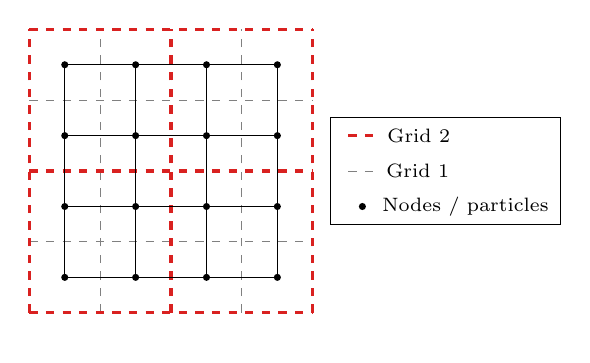
\begin{tikzpicture}[scale=0.9]
  \draw (0,0) --(3,0)--(3,3)--(0,3)--(0,0);
  \draw[white] (0.,0) -- (0,-0.8);
  %%% Grid 1
  \foreach \y in {-0.5,0.5,...,3.5} 
  \draw[dashed,gray] (-0.5,\y) -- (3.5,\y);
  \foreach \x in {-0.5,0.5,...,3.5} 
  \draw[dashed,gray] (\x,-0.5) -- (\x,3.5);
  %%% Grid 2
  \foreach \y in {-0.5,1.5,...,3.5} 
  \draw[dashed,Red,very thick] (-0.5,\y) -- (3.5,\y);
  \foreach \x in {-0.5,1.5,...,3.5} 
  \draw[dashed,Red,very thick] (\x,-0.5) -- (\x,3.5);
  \foreach \y in {0.,1.,...,3.} 
  \foreach \x in {0.,1.,...,3.} 
  \fill (\x,\y) circle(0.05);
  \foreach \y in {0.,1.,...,3.} 
  \draw (0,\y) -- (3.,\y);
  \foreach \x in {0.,1.,...,3.} 
  \draw (\x,0) -- (\x,3);
  \draw (3.75,0.75) rectangle (7.,2.25);
  \fill (4.2,1.) circle (0.05) node [right] {\scriptsize$ \: \: \text{Nodes / particles}$};
  \draw[dashed,gray] (4.,1.5) -- (4.4,1.5) node [right] {\scriptsize$\color{black} \text{Grid 1}$};
  \draw[dashed,very thick,Red] (4.,2.) -- (4.4,2.) node [right] {\scriptsize$\color{black} \text{Grid 2}$};
\end{tikzpicture}


%%% Local Variables:
%%% mode: latex
%%% TeX-master: "../manuscript"
%%% End:
}
  \caption{Geometry, loading and boundary conditions for the tensile impact problem on a two-dimensional elastic medium. The initial velocity is set to $v_d=-200 \: m/s$.}
  \label{fig:PS_domain}
\end{figure}
It is worth noticing that this simulation enables comparisons between the numerical methods in spite of the lack of exact solution for that problem.
Unfortunately, this cannot be circumvented by taking a FEM solution on a very fine mesh as the reference one since, as mentioned in section \ref{sec:plane-strain-problem}, a refinement does not prevent from spurious oscillations and hence, from an overestimation of the plastic strain.



Comparisons of the isovalues of longitudinal PK1 stress $\Pi_{11}$ and cumulated plastic strain $p$ are depicted in figures \ref{subfig:stress_comparison} and \ref{subfig:epls_comparison} respectively for two time steps that correspond to the incident and reflected pressure waves.
The fields are plotted on the current configuration so as to show the deformed shape resulting from each simulation.
Notice that a mesh is reconstructed based on the material points for MPM and DGMPM results for vizualisation purpose.

Before the reflection of the pressure wave, the arising of spurious oscillations arising in MPM and FEM solutions, though much slighter in the latter, and of numerical diffusion in DGMPM(4ppc) one, leads to different assessement of fields.
In addition to the stress peaks occuring in the MPM stress solution in the bottom part of the domain, a checkerboard structure can be seen upstream.
Then, figure \ref{subfig:epls_comparison} shows that the numerical cumulated plastic strains have globally the same shape but different extreme values.

Next, the incident wave reflects on the right end of the solid as a tensile wave so that the bottom part of the boundary starts moving rightward.
After that reflection, similar observations can be made about the MPM and the DGMPM(4ppc) stress solutions, that is, significant oscillations and numerical diffusion respectively.
Moreover, although the FEM and DGMPM(1ppc) stresses are quite similar before the reflection, it is no longer the case after the passage of the tensile wave so that the FEM solution exhibit a maximum that is higher than DGMPM one.
On the other hand, the plastic continues propagating within the domain and no significant difference appears in the numerical cumulated plastic strains.
At that time, it can also be seen that the shapes of the solid domain are quite similar, even though DGMPM solutions leads to a slightly lower vertical displacement of the top left corner of the square.
\begin{figure}[ht]
  \centering
  \subcaptionbox{Stress \label{subfig:stress_comparison}}{\begin{tikzpicture}[scale=1]
  \begin{groupplot}[group style={group size=2 by 4,% columns by rows
      ylabels at=edge left, yticklabels at=edge left,
      horizontal sep=5.ex,
      vertical sep=2ex,},
    enlargelimits=0,
    xmin=0.,xmax=1., ymin=-0.,ymax=1.
    ,axis on top,scale only axis,width=0.18\linewidth
    ,xtick=\empty,ytick=\empty,
    colorbar style={
      title style={
        font=\normalsize,
        at={(1,.5)},
        anchor=north west
      },yticklabel style={font=\normalsize}
      ,at={(current axis.south east)},anchor=south west
    },colormap name=tol
    ]
    %% FIRST ROW (time 1 = 5.10e-4s)
    %%% RANGE -8.6e9 -- 0.57e9
    \nextgroupplot[title={$t=5.10\times 10^{-4} \:s$},ylabel={FEM}]\addplot graphics[xmin=0.,xmax=1., ymin=-0.,ymax=1.] {pngFigures/fem_stress1-crop.png};
    \nextgroupplot[title={$t=1.02\times 10^{-3} \:s$}]\addplot graphics[xmin=0.,xmax=1., ymin=-0.,ymax=1.] {pngFigures/fem_stress2-crop.png};

    \nextgroupplot[ylabel={MPM(1ppc)}]\addplot graphics[xmin=0.,xmax=1., ymin=-0.,ymax=1.] {pngFigures/mpm_stress1-crop.png};
    \nextgroupplot[]\addplot graphics[xmin=0.,xmax=1., ymin=-0.,ymax=1.] {pngFigures/mpm_stress2-crop.png};

    \nextgroupplot[ylabel={DGMPM(1ppc)}]\addplot graphics[xmin=0.,xmax=1., ymin=-0.,ymax=1.] {pngFigures/dgmpm1ppc_stress1-crop.png};
    \nextgroupplot[]\addplot graphics[xmin=0.,xmax=1., ymin=-0.,ymax=1.] {pngFigures/dgmpm1ppc_stress2-crop.png};
    

    \nextgroupplot[ylabel={DGMPM(4ppc)},colorbar horizontal,colorbar  style={
      title style={yshift=-1.5cm},
      title= {$\Pi_{11}\: (GPa)$},
      xtick={-8.6,0.57},
      xticklabels={-8.6,0.57},
    }]
    \addplot[scatter,scatter src=x,mark size=0.pt] coordinates {(-8.6,0.) (0.57,0)};% Fake extreme values to fix scale
    \addplot graphics[xmin=0.,xmax=1., ymin=-0.,ymax=1.] {pngFigures/dgmpm4ppc_stress1-crop.png};
    \nextgroupplot[colorbar horizontal,colorbar  style={
      title style={yshift=-1.5cm},
      title= {$\Pi_{11}\: (GPa)$},
      xtick={-2.3,5.6},
      xticklabels={-2.3,5.6},
    }]
    \addplot[scatter,scatter src=x,mark size=0.pt] coordinates {(-2.3,0.) (5.6,0)};% Fake extreme values to fix scale
    \addplot graphics[xmin=0.,xmax=1., ymin=-0.,ymax=1.] {pngFigures/dgmpm4ppc_stress2-crop.png};
    
  \end{groupplot}
\end{tikzpicture}



%%% Local Variables:
%%% mode: latex
%%% TeX-master: "../manuscript"
%%% End:
}\qquad
  \subcaptionbox{Cumulated plastic strain \label{subfig:epls_comparison}}{\begin{tikzpicture}[scale=1]
  \begin{groupplot}[group style={group size=2 by 4,% columns by rows
      ylabels at=edge left, yticklabels at=edge left,
      horizontal sep=5.ex,
      vertical sep=2ex,},
    enlargelimits=0,
    xmin=0.,xmax=1., ymin=-0.,ymax=1.
    ,axis on top,scale only axis,xtick=\empty,ytick=\empty,width=0.18\linewidth,
    colorbar style={
      title style={
        font=\normalsize,
        at={(1,.5)},
        anchor=north west
      },yticklabel style={font=\normalsize}
      ,at={(current axis.south east)},anchor=south west
    },colormap name=tol]
    %% FIRST ROW (time 1 = 5.10e-4s)
    %%% RANGE -8.6e9 -- 0.57e9
    \nextgroupplot[title={$t=5.10\times 10^{-4} \:s$},ylabel={FEM}]\addplot graphics[xmin=0.,xmax=1., ymin=-0.,ymax=1.] {pngFigures/fem_epeq1-crop.png};
    \nextgroupplot[title={$t=1.02\times 10^{-3} \:s$}]\addplot graphics[xmin=0.,xmax=1., ymin=-0.,ymax=1.] {pngFigures/fem_epeq2-crop.png};

    \nextgroupplot[ylabel={MPM(1ppc)}]\addplot graphics[xmin=0.,xmax=1., ymin=-0.,ymax=1.] {pngFigures/mpm_epeq1-crop.png};
    \nextgroupplot[]\addplot graphics[xmin=0.,xmax=1., ymin=-0.,ymax=1.] {pngFigures/mpm_epeq2-crop.png};

    \nextgroupplot[ylabel={DGMPM(1ppc)}]\addplot graphics[xmin=0.,xmax=1., ymin=-0.,ymax=1.] {pngFigures/dgmpm1ppc_epeq1-crop.png};
    \nextgroupplot[]\addplot graphics[xmin=0.,xmax=1., ymin=-0.,ymax=1.] {pngFigures/dgmpm1ppc_epeq2-crop.png};
    

    \nextgroupplot[ylabel={DGMPM(4ppc)},colorbar horizontal,colorbar  style={
      title style={yshift=-1.5cm},
      title= {$p$},
      xtick={0,.15},
      xticklabels={0,0.15},
    }]
    \addplot[scatter,scatter src=x,mark size=0.pt] coordinates {(0,0.) (0.15,0)};% Fake extreme values to fix scale
    \addplot graphics[xmin=0.,xmax=1., ymin=-0.,ymax=1.] {pngFigures/dgmpm4ppc_epeq1-crop.png};
    \nextgroupplot[colorbar horizontal,colorbar  style={
      title style={yshift=-1.5cm},
      title= {$p$},
      xtick={0.,0.16},
      xticklabels={0,0.16},
    }]
    \addplot[scatter,scatter src=x,mark size=0.pt] coordinates {(0.,0.) (0.16,0)};% Fake extreme values to fix scale
    \addplot graphics[xmin=0.,xmax=1., ymin=-0.,ymax=1.] {pngFigures/dgmpm4ppc_epeq2-crop.png};
    
  \end{groupplot}
\end{tikzpicture}



%%% Local Variables:
%%% mode: latex
%%% TeX-master: "../manuscript"
%%% End:
}
  \caption{Isovalues of the PK1 stress tensor component $\Pi_{11}$ and cumulated plastic strain in a two-dimensional hyperelastic-plastic solids impacting a rigid wall under plane strain. Comparison of FEM (CFL=0.9), MPM (CFL=0.7) and DGMPM solutions using either one particle per cell (CFL=1) or four particles per cell (CFL=0.4).}
  \label{fig:PS_taylor}
\end{figure}

We now propose to look at the above results in more details.
Figures \ref{fig:bottom_line} and \ref{fig:left_line} show the evolution of longitudinal stress and cumulated plastic strain along the bottom and left end of the domain respectively for the same time steps.
First, it can be seen in figure \ref{subfig:bottom1} that the incident wave is described with different level of sharpness by the numerical shemes.
% Note however that no elastic predictor is seen in the stress profiles in contrast to the one-dimensional problem studied above.
Then, the figure also shows the oscillations in the MPM stress solution mentioned above.
Moreover, the superimposition of the stresses resulting from MPM computations using 1ppc or 4ppc shows that refining the particles discretization does not allow removing the numerical noise.
As a consequence, the numerical cumulated plastic strains near the wave front are rather different since the solutions of particle-based methods are ahead of the FEM one.
Upstream that front, the MPM(1ppc) plastic strain exhibits some peaks while this computed with the MPM(4ppc) is closer to the finite element solution.
On the other hand, the two space discretizations lead to DGMPM results that are close from one to another on the plastic plateau.

After the reflection (figure \ref{subfig:bottom2}), the stress profiles are much more different.
The MPM still yields oscillating solutions regardless the space discretization used, and DGMPM results are smoother than the other.
Once Again, the FEM leads to a rather sharp solution.
\begin{figure}[ht]
  \centering
  {\phantomsubcaption{\label{subfig:bottom1}}}
  {\phantomsubcaption{\label{subfig:bottom2}}}
  \begin{tikzpicture}
  \begin{groupplot}[group style={group size=2 by 2, % 3 columns 2 rows
      ylabels at=edge left, yticklabels at=edge left,horizontal sep=2.ex,vertical sep=5.ex,
      xticklabels at=edge bottom,xlabels at=edge bottom},
    ymajorgrids=true,xmajorgrids=true,
    axis on top,scale only axis,width=0.425\linewidth, every x tick scale label/.style={at={(xticklabel* cs:1.05,0.75cm)},anchor=near yticklabel},
    every y tick scale label/.style={at={(yticklabel* cs:1.05,-.9cm)},anchor=near yticklabel}]
    
    %%%%%%%%%%%%%%%%%%%% 
    % ============================== Stress Line
    % t1 
    \nextgroupplot[ylabel=$\Pi_{11} \:(Pa)$,title={(a) $t = 5.10 \times 10^{-4}\: s$},ymin=-1.e10,ymax=7.25e9]
    \addplot[Orange,thick,mark=*,mark repeat=2] table[x=Points:0,y=Piola_Stress:0] {csvFiles/fem_bottom1.csv};
    \addplot[Red,thick,mark=square,only marks] table[x=Points:0,y=Piola:0] {csvFiles/mpm_bottom1.csv};
    \addplot[black!60,thick,mark=o,only marks] table[x=Points:0,y=Piola:0] {csvFiles/mpm4ppc_bottom1.csv};
    \addplot[Blue,thick,mark=asterisk,only marks,mark size=3pt] table[x=Points:0,y=PK1:0] {csvFiles/dgmpm1ppc_bottom1.csv};
    \addplot[Purple,thick,mark=x,only marks,mark size=3pt,mark repeat=2] table[x=Points:0,y=PK1:0] {csvFiles/dgmpm4ppc_bottom1.csv};
    
    % t2 
    \nextgroupplot[title={(b) $t = 1.02 \times 10^{-3}\: s$},ymin=-1.e10,ymax=7.25e9%,ymin=-7.5e9,ymax=100.e9,ytick scale label code/.code={},legend style={at={($(0.75,-0.4)+(0.9cm,0.6cm)$)},legend columns=3}
    ]
    \addplot[Orange,thick,mark=*,mark repeat=2] table[x=Points:0,y=Piola_Stress:0] {csvFiles/fem_bottom2.csv};
    \addplot[Red,thick,mark=square,only marks] table[x=Points:0,y=Piola:0] {csvFiles/mpm_bottom2.csv};
    \addplot[black!60,thick,mark=o,only marks] table[x=Points:0,y=Piola:0] {csvFiles/mpm4ppc_bottom2.csv};
    \addplot[Blue,thick,mark=asterisk,only marks,mark size=3pt] table[x=Points:0,y=PK1:0] {csvFiles/dgmpm1ppc_bottom2.csv};
    \addplot[Purple,thick,mark=x,only marks,mark size=3pt,mark repeat=2] table[x=Points:0,y=PK1:0] {csvFiles/dgmpm4ppc_bottom2.csv};


    % ============================== Cumulated plastic strain Line
    % t1 
    \nextgroupplot[ylabel=$p$,xlabel=$x \: (m)$,ymin=0.,ymax=9.e-2%,ymin=-7.5e9,ymax=100.e9,ytick scale label code/.code={}
    ]
    \addplot[Orange,thick,mark=*,mark repeat=2] table[x=Points:0,y=Equivalent_Plastic_Strain] {csvFiles/fem_bottom1.csv};
    \addplot[Red,thick,mark=square,only marks] table[x=Points:0,y=epeq] {csvFiles/mpm_bottom1.csv};
    \addplot[black!60,thick,mark=o,only marks] table[x=Points:0,y=epeq] {csvFiles/mpm4ppc_bottom1.csv};
    \addplot[Blue,thick,mark=asterisk,only marks,mark size=3pt] table[x=Points:0,y=epeq] {csvFiles/dgmpm1ppc_bottom1.csv};
    \addplot[Purple,thick,mark=x,only marks,mark size=3pt,mark repeat=2] table[x=Points:0,y=epeq] {csvFiles/dgmpm4ppc_bottom1.csv};
    
    % t2
    \nextgroupplot[legend style={at={($(0.75,-0.35)+(0.cm,1cm)$)},legend columns=5},xlabel=$x \: (m)$,ymin=0.,ymax=9.e-2%,ymin=-7.5e9,ymax=100.e9,ytick scale label code/.code={}
    ]
    \addplot[Orange,thick,mark=*,mark repeat=2] table[x=Points:0,y=Equivalent_Plastic_Strain] {csvFiles/fem_bottom2.csv};
    \addplot[black!60,thick,mark=o,only marks] table[x=Points:0,y=epeq] {csvFiles/mpm_bottom2.csv};
    \addplot[Red,thick,mark=square,only marks] table[x=Points:0,y=epeq] {csvFiles/mpm4ppc_bottom2.csv};
    \addplot[Blue,thick,mark=asterisk,only marks,mark size=3pt] table[x=Points:0,y=epeq] {csvFiles/dgmpm1ppc_bottom2.csv};
    \addplot[Purple,thick,mark=x,only marks,mark size=3pt,mark repeat=2] table[x=Points:0,y=epeq] {csvFiles/dgmpm4ppc_bottom2.csv};

    \addlegendentry{fem \:}
    \addlegendentry{mpm (1ppc) \:}
    \addlegendentry{mpm (4ppc) \:}
    \addlegendentry{dgmpm (1ppc) \:}
    \addlegendentry{dgmpm (4ppc) \:}
    
    
  \end{groupplot}
\end{tikzpicture}



%%% Local Variables:
%%% mode: latex
%%% TeX-master: "../manuscript"
%%% End:

  \caption{Comparison of the longitudinal stress component and cumulated plastic strain along the bottom boundary of the domain at two times.}
  \label{fig:bottom_line}
\end{figure}
Furthermore, the MPM cumulated plastic strain curves oscillate around the FEM one which, in turn, is above these computed with the DGMPM.

The above observations are even more significant when looking at the evolution of fields along the left end of the square (figure \ref{fig:left_line}).
In figure \ref{subfig:left1}, FEM and DGMPM stress profiles show good agreement while spurious oscillations pollute MPM ones. 
Although FEM and DGMPM stresses are similar, it is not the case for the cumulated plastic strains for which the numerical results differ more.
Thus, the MPM yields the highest values of cumulated plastic strain at the top left corner of the domain.
The results depicted at the subsequent time show tremendous oscillations in the MPM(1ppc) solution for which the longitudinal stress varies roughly from $-7 \: GPa$ to $1 \: GPa$ in the bottom part of the left boundary.
These oscillations are reduced, though not completely removed, in the MPM(4ppc) results. 
On the other hand, DGMPM and FEM solutions no longer fit.
\begin{figure}[ht]
  \centering
  {\phantomsubcaption{\label{subfig:left1}}}
  {\phantomsubcaption{\label{subfig:left2}}}
  \input{pgfFigures/left_line}
  \caption{Comparison of the longitudinal stress component and cumulated plastic strain along the left boundary of the domain at two times.}
  \label{fig:left_line}
\end{figure}
It appears that the stress curve corresponding to the latter is bounded by these of the DGMPM(4ppc) and DGMPM(1ppc), the lower bound being given by the single particle space discretization.
At last, the cumulated plastic strain curves show similar behaviors to those of the previous time step except close to the bottom left corner of the domain.
In that region, the plastic flow developed differently depending on the numerical solution considered.
Both DGMPM curves are below that computed with the FEM while the profiles resulting from MPM computations are less regular than the other.

\subsection{Non-linear hardening material}
\label{sec:non-linear-hardening}
Reprendre le cas test hyperelastique de la these?


%%% Local Variables:
%%% mode: latex
%%% TeX-master: "manuscript"
%%% End:


% \section{Towards a two-dimensional elastoplastic Riemann solver}
% \label{sec:ep_Riemman_solver}
% Commencer par un résumé du ce qui a été identifié au dessus.

Eventuellement ne parler que d'un cas pour lequel c'est plus simple comme les defs planes (encore que...).

On pourrait faire comme Lin et Ballman \cite{Lin_et_Ballman} en se donnant 3 composantes de contraintes et en intégrant. 
C'est ce qui paraît le plus faisable dans l'état. 
Sauf que sigma22 fout la merde à cause car on a 3 inconnues en contraintes alors que pour le thin-walled tube on en n'avait que 2 et on pouvait itérer comme ça.
En effet, les interscetions dans les plans u,sigma et v,tau des courbes intégrales nous donnait des nouveaux états de contraintes pour l'étape d'après. 
Qu'en est-il avec sigma22 ?


Pour un solveur approximé:
Identifier le trajet ?? A priori, on ne peut pas sans intégrer.
Sauf si on fait une projection radiale de l'état trial sur le critère et qu'on cherche quelle onde part de là.
Il semblerait tout de même que la plasticité est surtout répendue par les ondes slow.
Les ondes fast font tourner autour du critère. 
Clifton suppose qu'elles n'existent que si leurs point de départ est à tau=0. On peut faire la même chose ?
On peut approximer les trajets par la tangente sur le critère pour les ondes slow.
%% Tracer des structures charactéristiques (revoir dans la biblio où on met une discontinuité et où on n'en met pas)








%%% Local Variables:
%%% mode: latex
%%% TeX-master: "../mainManuscript"
%%% End:



\section*{Conclusion}

\subsection*{Summary of the chapter}

In this chapter, the characteristic structure of the solution of hyperbolic problems in elastic-plastic solids in two space dimensions has been highlighted.
It is known since the 50s that plastic flow in two-dimensional solids yields two families of waves which speeds depend on the stress state, the slow and fast waves.
As a result, shock and simple waves may occur in an elastoplastic medium even for linear hardening material.
In addition, these plastic waves may have an impact on several stresses in contrast to elastic discontinuities across which one stress component varies, hence the name of combined stress waves.
During the 60s, attention has been paid to simple waves in particular two-dimensional problems thus providing, among other, solutions of Picard problems in elastic-plastic medium undergoing step loadings \cite{Clifton,Ting68,Ting73}. % Idem pour ting ? c'est dit dans l'intro ? voir ce qui est fait dans le 73
The singular nature of such problems lies in the fact that the characteristic structure of the solution depends on the external loading undergone.
Indeed, it has been shown \cite{Clifton} that boundary conditions can lead to plastic flow involving one fast, one slow, or both simple waves.
Therefore, it is crucial to be able to identify typical stress paths followed in each simple waves in order to link the initial data to a given stress state, and subsequently to determine the occurring wave pattern.

$\newline$
%% Lin et Ballman
Based on those works, an iterative Riemann solver \cite{Lin_et_Ballman}, which procedure has been recalled in section \ref{sec:stress_paths_num}, has been developed for the numerical solution of the thin-walled tube problem. 
% L'idée ici c'est de généraliser cette approche pour tous les problèmes 2D
Following this approach, identifying characteristic wave patterns for general elastoplastic problems in two space dimensions should allow to enrich the numerical solution with the knowledge of physics.
For that purpose, the characteristic analysis of two-dimensional problems in elastic-plastic materials with linear isotropic hardening under plane strain and plane stress, in projection in an arbitrary direction of space, has been carried out in section \ref{sec:charac_plast}.
Fast and slow waves are also involved in the solution so that applying the method of characteristic through the simple waves provides a system of ODE.
Integration of this system leads to combined stress paths that are followed between initial and final stress states on the one hand, and to the integral curves in terms of velocity components involving integral along those loading paths on the other hand.
Specializing the ODEs to one direction of a Cartesian grid, it has been shown in section \ref{sec:stress_paths} that the loading paths satisfied through slow and fast waves are perpendicular in the stress space for both plane strain and plaen stress.
Moreover, it has been established that the stress paths exhibit particular behavior in the space $(\sigma_{11},\sigma_{22},\sigma_{12})$, that is $d\sigma_{11}=0$, $d\sigma_{12}=0$ or $d\sigma_{22}=0$, for special values of the components of the acoustic tensor.
These situations are achieved for different stress states depending on wheter the problem involves plane stresses of plane strains as shown in section \ref{sec:stress_paths}.

$\newline$
The complexity of the ODEs derived in section \ref{sec:charac_plast} prevents from identifying all the singularities which may occur along the loading paths.
Hence, the mathematical analysis has been supplemented with numerical results consisting in the integration of stress paths from arbitrary initial stress values lying on the initial yield surface, for the particular direction of space $\vect{e}_1$.

%% Thin-walled tube
First, in section \ref{sec:num_thin-walled} the loading paths resulting from the integration of the ODEs derived in section \ref{sec:charac_plast} have been compared to those of Clifton \cite{Clifton}.
The two different formulations, respectively based on elastoplastic stiffnesses and softnesses, show a good agreement.

%% Cont. planes
Second, some the evolution of stress components across fast and slow waves under plane stress has been looked at in section \ref{sec:num_plane_stress}.
It appears that though the loading paths are rather complex in stress space through a fast wave, the stress evolution in the deviatoric plane is restricted to the initial yield surface until one direction of pure shear is reached.
A singularity then occurs so that the numerical integration cannot be pursued.
On the other hand, the loading paths resulting from the integration of ODEs satisfied inside a slow wave, except that $\sigma_{11}$ varies much less than the other stress components.

%% Def. planes
Third, the plane strain case has been considered in section \ref{sec:num_plane_strain}.
Once again, the integral curves inside a fast wave show complex shapes in stress space, and an evolution restricted to the initial yield surface in the deviatoric plane.
In that case, however, the paths may follow a direction of pure tensile/compression in the latter plane so that the plastic flow is radial. 
In contrast, the slow waves lead to a stress state of pure shear in the deviatoric plane.

\subsection*{Towards a two-dimensional elastoplastic Riemann solver}
The physical structures emphasized in this chapter enable a better understanding of the propagation of waves in two-dimensional elastoplastic medium, although further investigations are required.
On the other hand, the loading paths followed in fast and slow simple waves can be used in order to improve the numerical simulation of those problems.

%% Lin et Ballman
One possibility is to generalized the approach proposed by Lin and Ballman \cite{Lin_et_Ballman} based on the clues provided above.
The idea would be to successively assume stationary states of the Riemann problem in terms of stress $\sigma_{11}$, $\sigma_{12}$ and $\sigma_{22}$ in order to build stress paths starting from the initial data.
Namely, considering the direction $\vect{e}_1$, the loading paths followed through a fast wave can be integrated backward starting from the guess state.
Then, different situations may occur:
\begin{itemize}
\item[(1-a)] the curve thus obtained crosses the initial yield surface at a point where $\sigma_{22}$ satisfy the initial data.
  In that case, the elastic dicontinuities led to that stress state so that the characterisitc structure correspond to this depicted in figure \ref{fig:charac}\subref{subfig:charac1}.
\item[(1-b)] if on the other hand the point reached on the initial yield does not satisfy the initial stress $\sigma_{22}$, a fast wave is added in order to browse the initial yield surface until the initial data is recovered.
  This situation is depicted in figure \ref{fig:charac}\subref{subfig:charac2}.
\item[(2-a)] the curve resulting from the reverse integration across a slow wave intersects the plane $\sigma_{12}=0$.
  Then, assuming that the paths of slow waves are symmetric with respect to that plane, a fast wave is added in order to reach the initial yield surface at the initial value of $\sigma_{22}$.
  Indeed, the fast waves have been shown to yield horizontal path in the ($\sigma_{11},\sigma_{12}$) plane in such a way that only that type of wave enables to achieve the initial elastic convex.
  This also corresponds to figure \ref{fig:charac}\subref{subfig:charac2}.
\item[(2-b)] if at last, the guessed state is such that $\sigma_{12}=0$, a fast wave enables to reach the initial yield surface as depicted in figure \ref{fig:charac}\subref{subfig:charac3}.
\end{itemize}

\begin{figure}[h!]
  \centering
  \subcaptionbox{One slow wave \label{subfig:charac1}}{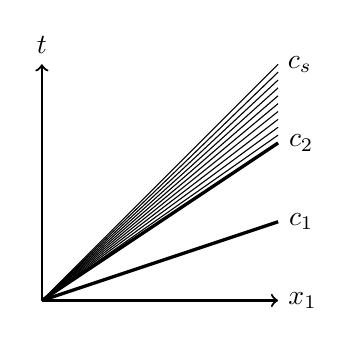
\begin{tikzpicture}
    \draw[thick, ->] (0,0) -- (3.,0) node [right] {$x_1$};
    \draw[thick, ->] (0,0) -- (0,3) node [above] {$t$};
    \draw[very thick] (0,0) -- (3,1) node [right] {$c_1$};
    \draw[very thick] (0,0) -- (3,2) node [right] {$c_2$};
    \foreach \x in {0.1,0.2,...,0.9}
    \draw (0,0) -- (3,2+\x);
    \draw (0,0) -- (3,3) node [right] {$c_s$};
\end{tikzpicture}} \qquad 
  \subcaptionbox{Both simple waves \label{subfig:charac2}}{\input{chapter5/pgfFigures/charac_structuresSlFa}} \qquad 
  \subcaptionbox{One fast wave \label{subfig:charac3}}{\input{chapter5/pgfFigures/charac_structuresFa}}
  \caption{Characteristic stuctures possibly occuring in two-dimensional elastic-plastic solids.}
  \label{fig:charac}
\end{figure}
Notice however that the above elementary loading paths are based on strong assumptions about the symmetry of the loading paths that have not been shown so far.
As a result, additional work must be performed in order to develop this approach and to introduce it in numerical methods.
Moreover, the hardening of the material may modifiy the behavior of the loading paths and have not been considered yet.
On the other hand, generalize the approach followed in this chapter to more complex hardening models (kinematic, nonlinear etc.) and other yield surfaces would be very interesting for the understanding of physics.
%On the other hand, generalized the approach followed in this chapter to more complex hardening models (kinematic, nonlinear etc.) and other yield surface would be of major interest for the understanding of physics.


%%% Local Variables:
%%% mode: latex
%%% TeX-master: "../mainManuscript"
%%% End:


%% Chapter 6: Contribution to the solution of two-dimensional elastoplastic problems
%%% Introduction:
The purpose of that work was the development of a numerical method allowing the accurate solution of hyperbolic problems in solid mechanics.
This class of mathematical problems governs the propagation of waves in finite deforming media.
Given the ability in dealing with large deformation enabled by meshless methods and the possiblity of describing discontinuous solutions provided by the DG approximation, it has been proposed to merge those to approaches.


%% Chapter2: Hyperbolic partial differential equations for solid dynamics


%% Chapter3: The Discontinuous Galerkin Material Point Method


%% Chapter4: Numerical Results


%% Chapter5: Contribution to the solution of elastic-plastic problems in two space dimensions



%%% Local Variables:
%%% mode: latex
%%% TeX-master: "../mainManuscript"
%%% End:



%% Chapter 7: Conclusion
%\input{chapter7/mainChapter7}


\bibliographystyle{apalike}
\bibliography{Biblio}

\end{document}

%%% Local Variables:
%%% mode: latex
%%% TeX-master: t
%%% End:
